We now move on to a problem involving three-dimensional stress states. Consider a infinite medium in directions $\vect{e}_2$ and $\vect{e}_3$ and of length $L=6\:m$ in direction $\vect{e}_1$. Riemann-type initial conditions similar to those treated above are assumed to yield the following infinitesimal strain and cauchy stress tensors:
\begin{align*}
  & \tens{\eps}= \eps \vect{e}_1 \otimes\vect{e}_1 \\
  & \tens{\sigma}=\sigma_L \vect{e}_1 \otimes \vect{e}_1 + \sigma_T \(\vect{e}_2 \otimes \vect{e}_2+\vect{e}_3 \otimes \vect{e}_3\) 
\end{align*}
which correspond to the plane wave assumption. In that case, a relation depending on the consitutive model considered exists between longitudinal and transverse stress componenents $\sigma_L$ and $\sigma_T$. As a consequence, a one-dimensional hyperbolic system is only solved for $\sigma_L=\sigma$ and the transverse componenent is computed subsequently. In this section, the behavior of the DGMPM on relaxation systems (see section \ref{sec:general-formulation}) is looked at by considering a solid medium made of a elastic-viscoplastic material with linear kinematic hardenings. In the asymptotic limit $\tau \rightarrow 0$, where $\tau$ is the relaxation time, the numerical solution must converge to that of elastoplastic materials that is studied afterwards. 
\begin{table}[h!]
  \centering
    \begin{tabular}{l|lN}
    \hline
    $E=2\times 10^{11}\:Pa$ & $\sigma^y=1 \times 10^8 Pa$ & \\ [3pt]
    $\nu=0.3$ & $C=10^{8} Pa$  &\\[3pt]
    $\rho_0 = 7800 \: kg.m^{-3}$ & &\\[3pt]
    \hline
  \end{tabular}

%%% Local Variables:
%%% mode: latex
%%% TeX-master: "../manuscript"
%%% End:

  \caption{Material parameters. The viscosity is expressed as a function of the relaxation time $\tau$.}
  \label{tab:material}
\end{table}
Table \ref{tab:material} lists the values of material parameters considered. In particular, the viscosity $\eta$ is a function of the relaxation time that is used to tune the stiffness of the problem.  
Finally, the initial velocity is set so that plastic flow occurs:
\begin{equation*}
  v_0=2\frac{Y_H}{\rho c_L}
\end{equation*}
where $Y_H=(\lambda+2\mu)/2\mu$ denotes the Hugoniot elastic limit and $c_L=\sqrt{(\lambda+2\mu)/\rho}$ is the elastic pressure wave speed.
% c=np.sqrt((lamb+2.*mu)/rho)
% hardening='kinematic'
% timeOut = 1.*length/c

% HEL = ((lamb+2.0*mu)/(2.0*mu))*Sigy
% v0=2.*HEL/(rho*c)
% algo = 'USL'
% update_position=False
% mpm_mapping=True
% limit=-1



\subsubsection{Elastoviscoplasticity}

Juste comparer DGMPM et MPM avec du strang et godunov 1ppc et 2ppc. Stiff $dt/tau=100$ non-stiff $dt/tau=1/50$ bdf3 pour strang. Pas de RK2 godunov car le RK2 n'a une influence que sur la partie convective qui est équivalent au 1ppc Euler.

\begin{figure}[h!]
  \centering
  % {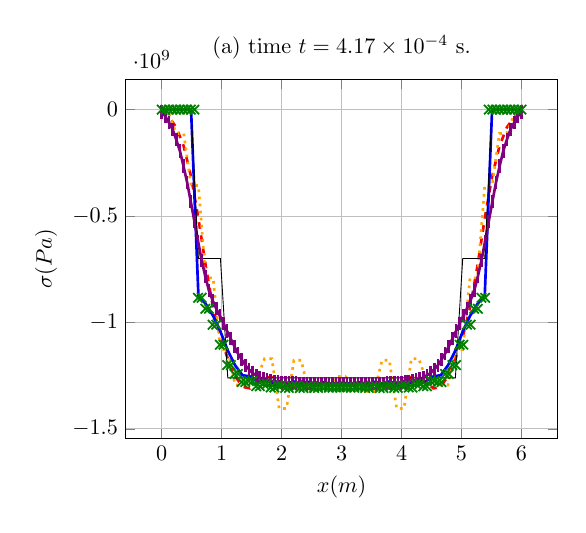
\begin{tikzpicture}[scale=0.8]
\begin{axis}[xlabel=$x (m)$,ylabel=$\sigma (Pa)$,ymajorgrids=true,xmajorgrids=true,legend pos=outer north east,title={(a) time $t = 4.17\times 10^{-4} $ s.}]
\addplot[Red,very thick,mark=none,dashed,mark size=3pt] coordinates {(0.0,-9466083.71137175) (0.12244897959183673,-35514206.734367736) (0.24489795918367346,-84113776.24908806) (0.36734693877551017,-172446629.58542818) (0.4897959183673469,-314805947.20807856) (0.6122448979591837,-511629446.98755276) (0.7346938775510203,-736313113.7069598) (0.8571428571428571,-931144828.2647986) (0.9795918367346939,-1068053644.3292406) (1.1020408163265305,-1170764300.0847378) (1.2244897959183674,-1252110103.6024575) (1.346938775510204,-1302676056.5462253) (1.4693877551020407,-1310165737.6186237) (1.5918367346938775,-1279757193.7171304) (1.7142857142857142,-1256553263.265204) (1.836734693877551,-1258006223.1072822) (1.9591836734693877,-1294050482.3234062) (2.0816326530612246,-1300642620.5987113) (2.204081632653061,-1307227334.5769467) (2.326530612244898,-1275303748.496001) (2.4489795918367347,-1289208797.7645764) (2.571428571428571,-1280826893.2226717) (2.693877551020408,-1303157436.709725) (2.816326530612245,-1289006021.9435475) (2.9387755102040813,-1289002398.658552) (3.061224489795918,-1289002460.452313) (3.183673469387755,-1289006071.890395) (3.306122448979592,-1303157225.279095) (3.4285714285714284,-1280827082.3206232) (3.5510204081632653,-1289208893.7221813) (3.673469387755102,-1275303766.5179212) (3.7959183673469385,-1307227387.3540978) (3.9183673469387754,-1300642664.183363) (4.040816326530612,-1294050357.0073159) (4.163265306122449,-1258006259.974342) (4.285714285714286,-1256553191.759347) (4.408163265306122,-1279757267.3487592) (4.530612244897959,-1310165771.052653) (4.653061224489796,-1302676007.627941) (4.775510204081632,-1252110079.6983936) (4.8979591836734695,-1170764547.776224) (5.020408163265306,-1068053501.3343573) (5.142857142857142,-931144730.4547592) (5.26530612244898,-736313057.6797745) (5.387755102040816,-511629430.76423925) (5.5102040816326525,-314805938.17461526) (5.63265306122449,-172446625.3783345) (5.755102040816326,-84113774.55431706) (5.877551020408163,-35514206.14830053) (6.0,-9466083.577332078) };
\addplot[Orange,very thick,mark=none,dotted,mark size=3pt] coordinates {(0.0,-21775616.685123403) (0.12244897959183673,-21775616.72164698) (0.24489795918367346,-112154769.91343763) (0.36734693877551017,-112154770.19419384) (0.4897959183673469,-357061973.86971843) (0.6122448979591837,-357061975.87384665) (0.7346938775510203,-790799603.3382715) (0.8571428571428571,-790799622.7090364) (0.9795918367346939,-1127863861.8971207) (1.1020408163265305,-1127863910.7156112) (1.2244897959183674,-1294097542.9943345) (1.346938775510204,-1294097833.9624486) (1.4693877551020407,-1264908473.5999227) (1.5918367346938775,-1264908907.9452155) (1.7142857142857142,-1170899419.842339) (1.836734693877551,-1170898869.1188018) (1.9591836734693877,-1404729307.196373) (2.0816326530612246,-1404729023.510617) (2.204081632653061,-1178030994.2246718) (2.326530612244898,-1178032103.900689) (2.4489795918367347,-1325532527.4682536) (2.571428571428571,-1325532662.4079945) (2.693877551020408,-1286992617.5223172) (2.816326530612245,-1286992228.933896) (2.9387755102040813,-1254505712.3434386) (3.061224489795918,-1254505904.1655023) (3.183673469387755,-1286992713.028294) (3.306122448979592,-1286993281.7005486) (3.4285714285714284,-1325532286.4512568) (3.5510204081632653,-1325532447.008532) (3.673469387755102,-1178031216.3396027) (3.7959183673469385,-1178031165.6288564) (3.9183673469387754,-1404729070.936975) (4.040816326530612,-1404729206.2986672) (4.163265306122449,-1170899488.2777543) (4.285714285714286,-1170899253.556783) (4.408163265306122,-1264908724.8211215) (4.530612244897959,-1264908806.5057957) (4.653061224489796,-1294097602.037558) (4.775510204081632,-1294097585.2606838) (4.8979591836734695,-1127863890.5307767) (5.020408163265306,-1127863857.5211554) (5.142857142857142,-790799615.9051313) (5.26530612244898,-790799601.5180427) (5.387755102040816,-357061976.4955751) (5.5102040816326525,-357061973.8588882) (5.63265306122449,-112154770.18131427) (5.755102040816326,-112154769.96143283) (5.877551020408163,-21775616.70163) (6.0,-21775616.698375184) };
\addplot[Blue,very thick,mark=none,solid,mark size=3pt] coordinates {(0.0,-6.648826343127885e-07) (0.12244897959183673,4.986619757345916e-07) (0.24489795918367346,-6.648826343127894e-07) (0.36734693877551017,6.648826343127889e-07) (0.4897959183673469,-3.324413171563951e-07) (0.6122448979591837,-874162257.8546059) (0.7346938775510203,-913424760.9782704) (0.8571428571428571,-969365384.6175718) (0.9795918367346939,-1042970790.4967976) (1.1020408163265305,-1132583339.8680727) (1.2244897959183674,-1201739241.5745146) (1.346938775510204,-1248614593.9146428) (1.4693877551020407,-1253812053.171889) (1.5918367346938775,-1277494278.936118) (1.7142857142857142,-1268975112.888906) (1.836734693877551,-1285312313.5954506) (1.9591836734693877,-1275249588.3375967) (2.0816326530612246,-1288549436.3162062) (2.204081632653061,-1278115488.7494104) (2.326530612244898,-1289609709.5365772) (2.4489795918367347,-1280020503.890194) (2.571428571428571,-1288883802.6033092) (2.693877551020408,-1282041862.894144) (2.816326530612245,-1286896451.527247) (2.9387755102040813,-1284697650.7072186) (3.061224489795918,-1284697650.7072196) (3.183673469387755,-1286896451.5272474) (3.306122448979592,-1282041862.8941436) (3.4285714285714284,-1288883802.6033094) (3.5510204081632653,-1280020503.890194) (3.673469387755102,-1289609709.5365787) (3.7959183673469385,-1278115488.74941) (3.9183673469387754,-1288549436.3162065) (4.040816326530612,-1275249588.337598) (4.163265306122449,-1285312313.5954502) (4.285714285714286,-1268975112.8889062) (4.408163265306122,-1277494278.9361184) (4.530612244897959,-1253812053.1718888) (4.653061224489796,-1248614593.914643) (4.775510204081632,-1201739241.5745142) (4.8979591836734695,-1132583339.8680727) (5.020408163265306,-1042970790.496798) (5.142857142857142,-969365384.6175721) (5.26530612244898,-913424760.9782704) (5.387755102040816,-874162257.8546067) (5.5102040816326525,6.648826343127891e-07) (5.63265306122449,-8.311032928909869e-07) (5.755102040816326,6.64882634312789e-07) (5.877551020408163,-4.986619757345927e-07) (6.0,6.648826343127891e-07) };
\addplot[Purple,very thick,mark=|,solid,mark size=3pt] coordinates {(0.0,-11522502.92600226) (0.06060606060606061,-31725620.091397233) (0.12121212121212122,-61304874.4765079) (0.18181818181818182,-93259931.32451278) (0.24242424242424243,-140838495.245558) (0.30303030303030304,-193913468.55103528) (0.36363636363636365,-265213878.38892987) (0.42424242424242425,-342130694.52595234) (0.48484848484848486,-432453677.3208593) (0.5454545454545454,-525041147.1169883) (0.6060606060606061,-618338331.152021) (0.6666666666666667,-708388503.4017504) (0.7272727272727273,-784021969.6614887) (0.7878787878787878,-850474949.5391626) (0.8484848484848485,-896076004.6724114) (0.9090909090909092,-935262643.3934776) (0.9696969696969697,-969337341.7916008) (1.0303030303030303,-1004304635.4591644) (1.0909090909090908,-1040567603.2284905) (1.1515151515151516,-1077307888.8979723) (1.2121212121212122,-1112635201.8637893) (1.2727272727272727,-1146677662.6062891) (1.3333333333333335,-1175184951.6380641) (1.393939393939394,-1201590500.124662) (1.4545454545454546,-1220740340.2067573) (1.5151515151515151,-1238089436.820448) (1.5757575757575757,-1249284876.1027403) (1.6363636363636365,-1259440830.6822593) (1.696969696969697,-1265589775.602502) (1.7575757575757576,-1271283785.6788774) (1.8181818181818183,-1274687789.8815384) (1.878787878787879,-1277922433.571672) (1.9393939393939394,-1279879339.775472) (2.0,-1281783669.6916373) (2.0606060606060606,-1282949267.7273479) (2.121212121212121,-1284109224.9776726) (2.1818181818181817,-1284819623.1742642) (2.2424242424242427,-1285544784.5476487) (2.303030303030303,-1285981972.386752) (2.3636363636363638,-1286442996.2191055) (2.4242424242424243,-1286710383.2766345) (2.484848484848485,-1287006241.599304) (2.5454545454545454,-1287165476.0382879) (2.606060606060606,-1287356422.5321994) (2.666666666666667,-1287445575.37196) (2.7272727272727275,-1287570603.4105794) (2.787878787878788,-1287613773.5740457) (2.8484848484848486,-1287701397.1398175) (2.909090909090909,-1287711163.0639696) (2.9696969696969697,-1287803837.1394258) (3.0303030303030303,-1287803837.1394258) (3.090909090909091,-1287711163.0639691) (3.1515151515151514,-1287701397.1398172) (3.2121212121212124,-1287613773.5740457) (3.272727272727273,-1287570603.4105797) (3.3333333333333335,-1287445575.37196) (3.393939393939394,-1287356422.5321996) (3.4545454545454546,-1287165476.038288) (3.515151515151515,-1287006241.5993047) (3.5757575757575757,-1286710383.276635) (3.6363636363636367,-1286442996.2191057) (3.6969696969696972,-1285981972.386752) (3.757575757575758,-1285544784.547649) (3.8181818181818183,-1284819623.1742642) (3.878787878787879,-1284109224.977673) (3.9393939393939394,-1282949267.7273483) (4.0,-1281783669.6916378) (4.0606060606060606,-1279879339.7754729) (4.121212121212121,-1277922433.571673) (4.181818181818182,-1274687789.881539) (4.242424242424242,-1271283785.678878) (4.303030303030303,-1265589775.602503) (4.363636363636363,-1259440830.6822598) (4.424242424242425,-1249284876.1027408) (4.484848484848485,-1238089436.8204484) (4.545454545454546,-1220740340.206758) (4.606060606060606,-1201590500.124663) (4.666666666666667,-1175184951.6380656) (4.7272727272727275,-1146677662.60629) (4.787878787878788,-1112635201.8637903) (4.848484848484849,-1077307888.8979728) (4.909090909090909,-1040567603.2284908) (4.96969696969697,-1004304635.459165) (5.03030303030303,-969337341.7916014) (5.090909090909091,-935262643.3934779) (5.151515151515151,-896076004.6724123) (5.212121212121212,-850474949.5391635) (5.2727272727272725,-784021969.6614897) (5.333333333333334,-708388503.401751) (5.3939393939393945,-618338331.1520219) (5.454545454545455,-525041147.11698914) (5.515151515151516,-432453677.3208602) (5.575757575757576,-342130694.5259528) (5.636363636363637,-265213878.3889301) (5.696969696969697,-193913468.55103546) (5.757575757575758,-140838495.24555832) (5.818181818181818,-93259931.3245125) (5.878787878787879,-61304874.4765082) (5.9393939393939394,-31725620.091397557) (6.0,-11522502.926002609) };
\addplot[Green,thick,mark=x,only marks,mark size=3pt] coordinates {(0.0,-2.0877147917780336e-07) (0.06060606060606061,-1.23669837978591e-07) (0.12121212121212122,1.0131895444177197e-06) (0.18181818181818182,9.814583585206487e-07) (0.24242424242424243,-5.619879278457838e-07) (0.30303030303030304,-7.677773407797948e-07) (0.36363636363636365,4.815476698956227e-07) (0.42424242424242425,1.8333496441716677e-07) (0.48484848484848486,1.0440135561077701e-07) (0.5454545454545454,2.2803996154561766e-07) (0.6060606060606061,-884550714.70502) (0.6666666666666667,-884550714.7050202) (0.7272727272727273,-936122014.0999393) (0.7878787878787878,-936122014.0999395) (0.8484848484848485,-1010904183.587626) (0.9090909090909092,-1010904183.5876261) (0.9696969696969697,-1105134845.294078) (1.0303030303030303,-1105134845.294077) (1.0909090909090908,-1200693543.9954407) (1.1515151515151516,-1200693543.9954407) (1.2121212121212122,-1242600895.2828481) (1.2727272727272727,-1242600895.2828481) (1.3333333333333335,-1280378553.9593801) (1.393939393939394,-1280378553.9593809) (1.4545454545454546,-1275721452.5659273) (1.5151515151515151,-1275721452.5659602) (1.5757575757575757,-1300299286.3908393) (1.6363636363636365,-1300299286.3908374) (1.696969696969697,-1289272425.5395763) (1.7575757575757576,-1289272425.5395694) (1.8181818181818183,-1306127301.5683103) (1.878787878787879,-1306127301.5683022) (1.9393939393939394,-1296028797.1903882) (2.0,-1296028797.1903853) (2.0606060606060606,-1308123608.354041) (2.121212121212121,-1308123608.3541112) (2.1818181818181817,-1299597735.2461388) (2.2424242424242427,-1299597735.246238) (2.303030303030303,-1308620980.1784377) (2.3636363636363638,-1308620980.1784313) (2.4242424242424243,-1301801281.3713925) (2.484848484848485,-1301801281.3713658) (2.5454545454545454,-1308121765.4283872) (2.606060606060606,-1308121765.4283755) (2.666666666666667,-1303587683.0677166) (2.7272727272727275,-1303587683.0677037) (2.787878787878788,-1306911469.4399674) (2.8484848484848486,-1306911469.4400563) (2.909090909090909,-1305310135.1663263) (2.9696969696969697,-1305310135.1662202) (3.0303030303030303,-1305310135.1663122) (3.090909090909091,-1305310135.1663315) (3.1515151515151514,-1306911469.4400697) (3.2121212121212124,-1306911469.4400973) (3.272727272727273,-1303587683.067521) (3.3333333333333335,-1303587683.0675333) (3.393939393939394,-1308121765.428341) (3.4545454545454546,-1308121765.4283326) (3.515151515151515,-1301801281.3712707) (3.5757575757575757,-1301801281.3712776) (3.6363636363636367,-1308620980.1785724) (3.6969696969696972,-1308620980.1785636) (3.757575757575758,-1299597735.2460728) (3.8181818181818183,-1299597735.2461448) (3.878787878787879,-1308123608.3541088) (3.9393939393939394,-1308123608.3540418) (4.0,-1296028797.1904147) (4.0606060606060606,-1296028797.190405) (4.121212121212121,-1306127301.5683162) (4.181818181818182,-1306127301.5683157) (4.242424242424242,-1289272425.5394864) (4.303030303030303,-1289272425.5394852) (4.363636363636363,-1300299286.390773) (4.424242424242425,-1300299286.3907716) (4.484848484848485,-1275721452.565949) (4.545454545454546,-1275721452.565983) (4.606060606060606,-1280378553.9593606) (4.666666666666667,-1280378553.9593616) (4.7272727272727275,-1242600895.2828217) (4.787878787878788,-1242600895.2828217) (4.848484848484849,-1200693543.9954677) (4.909090909090909,-1200693543.9954684) (4.96969696969697,-1105134845.294094) (5.03030303030303,-1105134845.2940938) (5.090909090909091,-1010904183.5876323) (5.151515151515151,-1010904183.5876321) (5.212121212121212,-936122014.0999426) (5.2727272727272725,-936122014.0999423) (5.333333333333334,-884550714.7050228) (5.3939393939393945,-884550714.7050234) (5.454545454545455,6.698192810303248e-07) (5.515151515151516,6.599459875952535e-07) (5.575757575757576,-9.369788715662316e-07) (5.636363636363637,-1.0576690313721361e-06) (5.696969696969697,1.675441116120912e-06) (5.757575757575758,1.6489720554430353e-06) (5.818181818181818,-1.0608989471845062e-06) (5.878787878787879,-9.337489557538617e-07) (5.9393939393939394,1.4751713795395358e-06) (6.0,1.5168004748680168e-06) };
\addplot[black,thin,mark=none,solid,mark size=3pt] coordinates {(0.0,-0.0) (0.12244897959183673,-0.0) (0.24489795918367346,-0.0) (0.36734693877551017,-0.0) (0.4897959183673469,-0.0) (0.6122448979591837,-700000000.0) (0.7346938775510203,-700000000.0) (0.8571428571428571,-700000000.0) (0.9795918367346939,-700000000.0) (1.1020408163265305,-1261004576.260559) (1.2244897959183674,-1261004576.260559) (1.346938775510204,-1261004576.260559) (1.4693877551020407,-1261004576.260559) (1.5918367346938775,-1261004576.260559) (1.7142857142857142,-1261004576.260559) (1.836734693877551,-1261004576.260559) (1.9591836734693877,-1261004576.260559) (2.0816326530612246,-1261004576.260559) (2.204081632653061,-1261004576.260559) (2.326530612244898,-1261004576.260559) (2.4489795918367347,-1261004576.260559) (2.571428571428571,-1261004576.260559) (2.693877551020408,-1261004576.260559) (2.816326530612245,-1261004576.260559) (2.9387755102040813,-1261004576.260559) (3.061224489795918,-1261004576.260559) (3.183673469387755,-1261004576.260559) (3.306122448979592,-1261004576.260559) (3.4285714285714284,-1261004576.260559) (3.5510204081632653,-1261004576.260559) (3.673469387755102,-1261004576.260559) (3.7959183673469385,-1261004576.260559) (3.9183673469387754,-1261004576.260559) (4.040816326530612,-1261004576.260559) (4.163265306122449,-1261004576.260559) (4.285714285714286,-1261004576.260559) (4.408163265306122,-1261004576.260559) (4.530612244897959,-1261004576.260559) (4.653061224489796,-1261004576.260559) (4.775510204081632,-1261004576.260559) (4.8979591836734695,-1261004576.260559) (5.020408163265306,-700000000.0) (5.142857142857142,-700000000.0) (5.26530612244898,-700000000.0) (5.387755102040816,-700000000.0) (5.5102040816326525,-0.0) (5.63265306122449,-0.0) (5.755102040816326,-0.0) (5.877551020408163,-0.0) (6.0,-0.0) };
%\legend{usl 1ppc,usf 1ppc,dgmpm 1ppc,dgmpm 2ppc,dgmpm 2ppc (RK2 + strang),plastic solution}
\end{axis}
\end{tikzpicture}
%%% Local Variables:
%%% mode: latex
%%% TeX-master: "../../mainManuscript"
%%% End:
}
  % {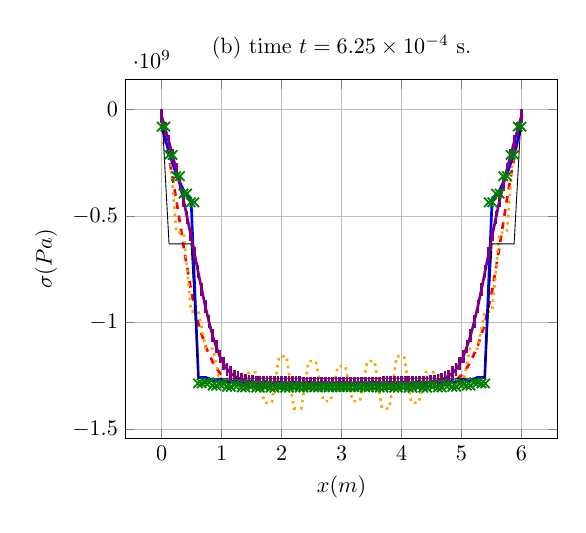
\begin{tikzpicture}[scale=0.8]
\begin{axis}[xlabel=$x (m)$,ylabel=$\sigma (Pa)$,ymajorgrids=true,xmajorgrids=true,legend pos=outer north east,title={(b) time $t = 6.25\times 10^{-4} $ s.}]
\addplot[Red,very thick,mark=none,dashed,mark size=3pt] coordinates {(0.0,-68320403.62221353) (0.12244897959183673,-225789676.02918974) (0.24489795918367346,-424791619.04833) (0.36734693877551017,-646380796.7713014) (0.4897959183673469,-849944016.2028724) (0.6122448979591837,-1006146061.0400205) (0.7346938775510203,-1114292580.0561018) (0.8571428571428571,-1188728982.2247245) (0.9795918367346939,-1241700251.4602263) (1.1020408163265305,-1273020972.5655205) (1.2244897959183674,-1284949093.1656094) (1.346938775510204,-1280762376.3082383) (1.4693877551020407,-1280131918.3035223) (1.5918367346938775,-1279490959.2062156) (1.7142857142857142,-1290763235.7380192) (1.836734693877551,-1286886471.7575386) (1.9591836734693877,-1293425757.5226574) (2.0816326530612246,-1281287553.8251324) (2.204081632653061,-1292409766.4422443) (2.326530612244898,-1282629752.438702) (2.4489795918367347,-1294945401.113779) (2.571428571428571,-1283794612.9732673) (2.693877551020408,-1291887694.9803798) (2.816326530612245,-1285785861.1559482) (2.9387755102040813,-1289860908.4664276) (3.061224489795918,-1289860960.9809775) (3.183673469387755,-1285785837.4934893) (3.306122448979592,-1291887487.9744287) (3.4285714285714284,-1283794664.8462174) (3.5510204081632653,-1294945447.7560375) (3.673469387755102,-1282629760.5221589) (3.7959183673469385,-1292409767.8294322) (3.9183673469387754,-1281287565.3495717) (4.040816326530612,-1293425764.3679597) (4.163265306122449,-1286886489.0287468) (4.285714285714286,-1290763226.34359) (4.408163265306122,-1279490965.7329388) (4.530612244897959,-1280131956.1996849) (4.653061224489796,-1280762451.4159694) (4.775510204081632,-1284949184.1714568) (4.8979591836734695,-1273020948.2916741) (5.020408163265306,-1241700137.1761186) (5.142857142857142,-1188728796.523432) (5.26530612244898,-1114292407.0488575) (5.387755102040816,-1006146274.5465661) (5.5102040816326525,-849944214.1880462) (5.63265306122449,-646381051.5707061) (5.755102040816326,-424791730.9041514) (5.877551020408163,-225789800.60525674) (6.0,-68320454.65089296) };
\addplot[Orange,very thick,mark=none,dotted,mark size=3pt] coordinates {(0.0,-156995048.72300234) (0.12244897959183673,-156995364.03184575) (0.24489795918367346,-578361553.8773596) (0.36734693877551017,-578361776.9652294) (0.4897959183673469,-947878572.789029) (0.6122448979591837,-947878629.0454134) (0.7346938775510203,-1122155365.9445817) (0.8571428571428571,-1122155222.890123) (0.9795918367346939,-1291825792.2012048) (1.1020408163265305,-1291825773.3810687) (1.2244897959183674,-1251635171.0476031) (1.346938775510204,-1251635100.0260744) (1.4693877551020407,-1232474111.1713145) (1.5918367346938775,-1232473886.0470812) (1.7142857142857142,-1376816804.9626572) (1.836734693877551,-1376817081.1171806) (1.9591836734693877,-1157922444.4640186) (2.0816326530612246,-1157922510.7665095) (2.204081632653061,-1403184236.5989518) (2.326530612244898,-1403184536.0603929) (2.4489795918367347,-1180859401.2507882) (2.571428571428571,-1180859508.133819) (2.693877551020408,-1368793239.5548983) (2.816326530612245,-1368793451.4344292) (2.9387755102040813,-1203835945.0107105) (3.061224489795918,-1203835622.7844667) (3.183673469387755,-1368793306.427742) (3.306122448979592,-1368793478.6580884) (3.4285714285714284,-1180859183.8880649) (3.5510204081632653,-1180859290.5038683) (3.673469387755102,-1403184136.6867287) (3.7959183673469385,-1403183761.77251) (3.9183673469387754,-1157922482.3658946) (4.040816326530612,-1157922352.2307622) (4.163265306122449,-1376817001.1907525) (4.285714285714286,-1376817315.2298005) (4.408163265306122,-1232474572.3256762) (4.530612244897959,-1232474451.4669452) (4.653061224489796,-1251634884.2142015) (4.775510204081632,-1251635269.3170545) (4.8979591836734695,-1291825665.5679488) (5.020408163265306,-1291825906.6643884) (5.142857142857142,-1122155225.5621386) (5.26530612244898,-1122155914.2048798) (5.387755102040816,-947878625.770502) (5.5102040816326525,-947877795.5933025) (5.63265306122449,-578361684.1093763) (5.755102040816326,-578362214.7513508) (5.877551020408163,-156995223.63768175) (6.0,-156995328.8817121) };
\addplot[Blue,very thick,mark=none,solid,mark size=3pt] coordinates {(0.0,-78094246.59211227) (0.12244897959183673,-202047177.96964124) (0.24489795918367346,-306454110.06972677) (0.36734693877551017,-380145390.26078814) (0.4897959183673469,-423404735.09272164) (0.6122448979591837,-1257853636.3109157) (0.7346938775510203,-1257085473.8466249) (0.8571428571428571,-1273738336.1650534) (0.9795918367346939,-1266172602.6079874) (1.1020408163265305,-1281249763.7189615) (1.2244897959183674,-1270901976.3756995) (1.346938775510204,-1284583664.611882) (1.4693877551020407,-1273997234.574172) (1.5918367346938775,-1285577300.0190902) (1.7142857142857142,-1276400493.5524273) (1.836734693877551,-1285417293.975184) (1.9591836734693877,-1278339664.6925926) (2.0816326530612246,-1284852686.1476386) (2.204081632653061,-1279850028.976812) (2.326530612244898,-1284238970.623943) (2.4489795918367347,-1280987011.9763784) (2.571428571428571,-1283670980.1448214) (2.693877551020408,-1281846768.3113825) (2.816326530612245,-1283114948.4817128) (2.9387755102040813,-1282695202.1981924) (3.061224489795918,-1282695202.1981914) (3.183673469387755,-1283114948.4817138) (3.306122448979592,-1281846768.3113823) (3.4285714285714284,-1283670980.1448233) (3.5510204081632653,-1280987011.9763772) (3.673469387755102,-1284238970.6239436) (3.7959183673469385,-1279850028.9768124) (3.9183673469387754,-1284852686.147639) (4.040816326530612,-1278339664.6925926) (4.163265306122449,-1285417293.9751842) (4.285714285714286,-1276400493.5524268) (4.408163265306122,-1285577300.0190902) (4.530612244897959,-1273997234.5741723) (4.653061224489796,-1284583664.6118824) (4.775510204081632,-1270901976.3757002) (4.8979591836734695,-1281249763.718962) (5.020408163265306,-1266172602.6079872) (5.142857142857142,-1273738336.1650534) (5.26530612244898,-1257085473.8466249) (5.387755102040816,-1257853636.3109152) (5.5102040816326525,-423404735.092723) (5.63265306122449,-380145390.2607865) (5.755102040816326,-306454110.0697275) (5.877551020408163,-202047177.96964) (6.0,-78094246.59211358) };
\addplot[Purple,very thick,mark=|,solid,mark size=3pt] coordinates {(0.0,-29927303.866736423) (0.06060606060606061,-91056397.63368599) (0.12121212121212122,-151613704.523153) (0.18181818181818182,-216112605.28132087) (0.24242424242424243,-280335641.2622369) (0.30303030303030304,-352344393.75337386) (0.36363636363636365,-424489613.7233627) (0.42424242424242425,-505847292.410384) (0.48484848484848486,-586999789.9597377) (0.5454545454545454,-673998041.6926832) (0.6060606060606061,-759351839.9800754) (0.6666666666666667,-843513643.4035325) (0.7272727272727273,-923946644.5385387) (0.7878787878787878,-995414783.6619084) (0.8484848484848485,-1061232446.5295665) (0.9090909090909092,-1113218962.1696506) (0.9696969696969697,-1159051731.4367843) (1.0303030303030303,-1191404581.2317898) (1.0909090909090908,-1218844186.0222213) (1.1515151515151516,-1236684855.8963497) (1.2121212121212122,-1251383919.797765) (1.2727272727272727,-1260493728.1975224) (1.3333333333333335,-1267812955.7854612) (1.393939393939394,-1272272932.5908973) (1.4545454545454546,-1275765921.540089) (1.5151515151515151,-1277936320.3680944) (1.5757575757575757,-1279592582.5775201) (1.6363636363636365,-1280693510.9832897) (1.696969696969697,-1281513981.0637147) (1.7575757575757576,-1282125151.9012914) (1.8181818181818183,-1282572071.178818) (1.878787878787879,-1282950867.4850798) (1.9393939393939394,-1283223494.4286144) (2.0,-1283480133.76503) (2.0606060606060606,-1283661506.7126255) (2.121212121212121,-1283844490.520339) (2.1818181818181817,-1283970476.588324) (2.2424242424242427,-1284103730.0809987) (2.303030303030303,-1284191946.2274148) (2.3636363636363638,-1284289437.5825508) (2.4242424242424243,-1284350224.7858446) (2.484848484848485,-1284421413.7540164) (2.5454545454545454,-1284461770.7762535) (2.606060606060606,-1284513746.332839) (2.666666666666667,-1284538764.3494127) (2.7272727272727275,-1284577367.2906) (2.787878787878788,-1284590745.1308227) (2.8484848484848486,-1284621851.9102542) (2.909090909090909,-1284624878.9151099) (2.9696969696969697,-1284663796.6518083) (3.0303030303030303,-1284663796.6518083) (3.090909090909091,-1284624878.9151099) (3.1515151515151514,-1284621851.9102545) (3.2121212121212124,-1284590745.1308224) (3.272727272727273,-1284577367.2906) (3.3333333333333335,-1284538764.3494127) (3.393939393939394,-1284513746.332839) (3.4545454545454546,-1284461770.7762532) (3.515151515151515,-1284421413.7540162) (3.5757575757575757,-1284350224.7858446) (3.6363636363636367,-1284289437.582551) (3.6969696969696972,-1284191946.227415) (3.757575757575758,-1284103730.0809991) (3.8181818181818183,-1283970476.5883245) (3.878787878787879,-1283844490.5203397) (3.9393939393939394,-1283661506.712626) (4.0,-1283480133.7650306) (4.0606060606060606,-1283223494.4286153) (4.121212121212121,-1282950867.4850807) (4.181818181818182,-1282572071.1788187) (4.242424242424242,-1282125151.901292) (4.303030303030303,-1281513981.0637155) (4.363636363636363,-1280693510.9832904) (4.424242424242425,-1279592582.577521) (4.484848484848485,-1277936320.3680952) (4.545454545454546,-1275765921.5400894) (4.606060606060606,-1272272932.5908978) (4.666666666666667,-1267812955.785462) (4.7272727272727275,-1260493728.1975229) (4.787878787878788,-1251383919.797766) (4.848484848484849,-1236684855.8963506) (4.909090909090909,-1218844186.0222228) (4.96969696969697,-1191404581.231791) (5.03030303030303,-1159051731.4367847) (5.090909090909091,-1113218962.169651) (5.151515151515151,-1061232446.529567) (5.212121212121212,-995414783.6619091) (5.2727272727272725,-923946644.5385387) (5.333333333333334,-843513643.4035326) (5.3939393939393945,-759351839.9800754) (5.454545454545455,-673998041.6926835) (5.515151515151516,-586999789.9597379) (5.575757575757576,-505847292.4103844) (5.636363636363637,-424489613.7233631) (5.696969696969697,-352344393.7533744) (5.757575757575758,-280335641.2622374) (5.818181818181818,-216112605.28132126) (5.878787878787879,-151613704.5231535) (5.9393939393939394,-91056397.63368621) (6.0,-29927303.86673645) };
\addplot[Green,thick,mark=x,only marks,mark size=3pt] coordinates {(0.0,-79916002.67055239) (0.06060606060606061,-79916002.67055224) (0.12121212121212122,-212751355.9722632) (0.18181818181818182,-212751355.97226292) (0.24242424242424243,-312518540.6021343) (0.30303030303030304,-312518540.60213417) (0.36363636363636365,-394252960.7380532) (0.42424242424242425,-394252960.73804915) (0.48484848484848486,-435228881.2798793) (0.5454545454545454,-435228881.27987766) (0.6060606060606061,-1285411981.4217432) (0.6666666666666667,-1285411981.4217405) (0.7272727272727273,-1280711603.3230183) (0.7878787878787878,-1280711603.3230135) (0.8484848484848485,-1295937493.3862524) (0.9090909090909092,-1295937493.3862624) (0.9696969696969697,-1287988489.6130652) (1.0303030303030303,-1287988489.6129992) (1.0909090909090908,-1301349142.6084783) (1.1515151515151516,-1301349142.6085305) (1.2121212121212122,-1292031977.182477) (1.2727272727272727,-1292031977.1824605) (1.3333333333333335,-1304158962.6097703) (1.393939393939394,-1304158962.609774) (1.4545454545454546,-1294615911.7133598) (1.5151515151515151,-1294615911.713364) (1.5757575757575757,-1305409469.234389) (1.6363636363636365,-1305409469.2343793) (1.696969696969697,-1296575097.169732) (1.7575757575757576,-1296575097.1696386) (1.8181818181818183,-1305694934.8057256) (1.878787878787879,-1305694934.8056414) (1.9393939393939394,-1298237888.1883545) (2.0,-1298237888.1883388) (2.0606060606060606,-1305422829.3343308) (2.121212121212121,-1305422829.3343291) (2.1818181818181817,-1299681183.8928425) (2.2424242424242427,-1299681183.8927386) (2.303030303030303,-1304867646.3713446) (2.3636363636363638,-1304867646.3713348) (2.4242424242424243,-1300902385.280055) (2.484848484848485,-1300902385.280057) (2.5454545454545454,-1304201666.8734922) (2.606060606060606,-1304201666.8733885) (2.666666666666667,-1301910986.9763758) (2.7272727272727275,-1301910986.9763756) (2.787878787878788,-1303498906.5357742) (2.8484848484848486,-1303498906.535786) (2.909090909090909,-1302755121.5435212) (2.9696969696969697,-1302755121.5435221) (3.0303030303030303,-1302755121.543637) (3.090909090909091,-1302755121.543634) (3.1515151515151514,-1303498906.5355883) (3.2121212121212124,-1303498906.5355833) (3.272727272727273,-1301910986.97636) (3.3333333333333335,-1301910986.9762814) (3.393939393939394,-1304201666.8734074) (3.4545454545454546,-1304201666.8733807) (3.515151515151515,-1300902385.280354) (3.5757575757575757,-1300902385.2803435) (3.6363636363636367,-1304867646.3712885) (3.6969696969696972,-1304867646.3712816) (3.757575757575758,-1299681183.8926687) (3.8181818181818183,-1299681183.8927484) (3.878787878787879,-1305422829.3345184) (3.9393939393939394,-1305422829.3345306) (4.0,-1298237888.1883025) (4.0606060606060606,-1298237888.1882656) (4.121212121212121,-1305694934.8057399) (4.181818181818182,-1305694934.8057516) (4.242424242424242,-1296575097.1697433) (4.303030303030303,-1296575097.1697195) (4.363636363636363,-1305409469.2346466) (4.424242424242425,-1305409469.2346435) (4.484848484848485,-1294615911.7133439) (4.545454545454546,-1294615911.713418) (4.606060606060606,-1304158962.609734) (4.666666666666667,-1304158962.6097326) (4.7272727272727275,-1292031977.1825411) (4.787878787878788,-1292031977.1825192) (4.848484848484849,-1301349142.6085944) (4.909090909090909,-1301349142.6086338) (4.96969696969697,-1287988489.6129642) (5.03030303030303,-1287988489.6129599) (5.090909090909091,-1295937493.3861973) (5.151515151515151,-1295937493.38624) (5.212121212121212,-1280711603.3229506) (5.2727272727272725,-1280711603.3229578) (5.333333333333334,-1285411981.4217515) (5.3939393939393945,-1285411981.4217482) (5.454545454545455,-435228881.27979714) (5.515151515151516,-435228881.2797981) (5.575757575757576,-394252960.7380172) (5.636363636363637,-394252960.7380113) (5.696969696969697,-312518540.6021377) (5.757575757575758,-312518540.6021374) (5.818181818181818,-212751355.9722441) (5.878787878787879,-212751355.97224396) (5.9393939393939394,-79916002.67054233) (6.0,-79916002.67054217) };
\addplot[black,thin,mark=none,solid,mark size=3pt] coordinates {(0.0,-0.0) (0.12244897959183673,-630502288.1302795) (0.24489795918367346,-630502288.1302795) (0.36734693877551017,-630502288.1302795) (0.4897959183673469,-630502288.1302795) (0.6122448979591837,-1261004576.260559) (0.7346938775510203,-1261004576.260559) (0.8571428571428571,-1261004576.260559) (0.9795918367346939,-1261004576.260559) (1.1020408163265305,-1261004576.260559) (1.2244897959183674,-1261004576.260559) (1.346938775510204,-1261004576.260559) (1.4693877551020407,-1261004576.260559) (1.5918367346938775,-1261004576.260559) (1.7142857142857142,-1261004576.260559) (1.836734693877551,-1261004576.260559) (1.9591836734693877,-1261004576.260559) (2.0816326530612246,-1261004576.260559) (2.204081632653061,-1261004576.260559) (2.326530612244898,-1261004576.260559) (2.4489795918367347,-1261004576.260559) (2.571428571428571,-1261004576.260559) (2.693877551020408,-1261004576.260559) (2.816326530612245,-1261004576.260559) (2.9387755102040813,-1261004576.260559) (3.061224489795918,-1261004576.260559) (3.183673469387755,-1261004576.260559) (3.306122448979592,-1261004576.260559) (3.4285714285714284,-1261004576.260559) (3.5510204081632653,-1261004576.260559) (3.673469387755102,-1261004576.260559) (3.7959183673469385,-1261004576.260559) (3.9183673469387754,-1261004576.260559) (4.040816326530612,-1261004576.260559) (4.163265306122449,-1261004576.260559) (4.285714285714286,-1261004576.260559) (4.408163265306122,-1261004576.260559) (4.530612244897959,-1261004576.260559) (4.653061224489796,-1261004576.260559) (4.775510204081632,-1261004576.260559) (4.8979591836734695,-1261004576.260559) (5.020408163265306,-1261004576.260559) (5.142857142857142,-1261004576.260559) (5.26530612244898,-1261004576.260559) (5.387755102040816,-1261004576.260559) (5.5102040816326525,-630502288.1302795) (5.63265306122449,-630502288.1302795) (5.755102040816326,-630502288.1302795) (5.877551020408163,-630502288.1302795) (6.0,-0.0) };
%\legend{usl 1ppc,usf 1ppc,dgmpm 1ppc,dgmpm 2ppc,dgmpm 2ppc (RK2 + strang),plastic solution}
\end{axis}
\end{tikzpicture}
%%% Local Variables:
%%% mode: latex
%%% TeX-master: "../../mainManuscript"
%%% End:
}
  % {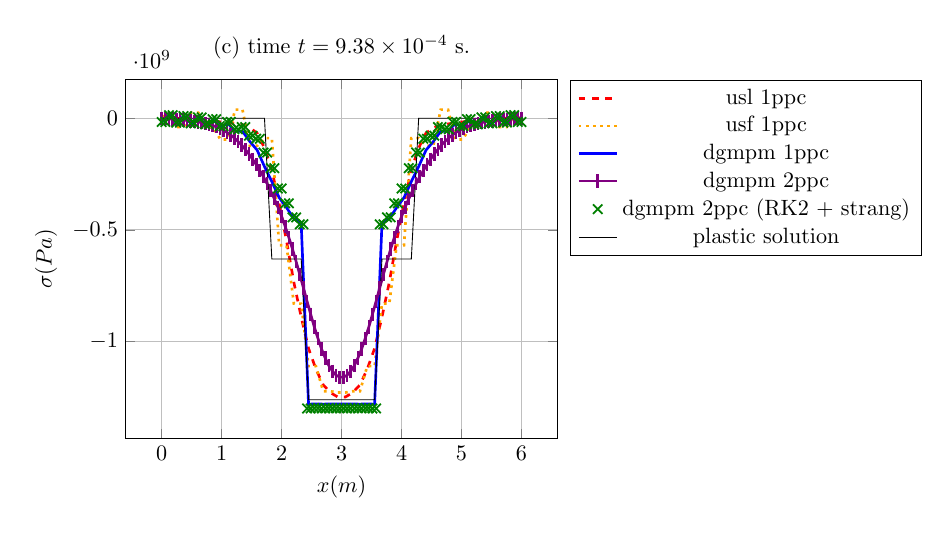
\begin{tikzpicture}[scale=0.8]
\begin{axis}[xlabel=$x (m)$,ylabel=$\sigma (Pa)$,ymajorgrids=true,xmajorgrids=true,legend pos=outer north east,title={(c) time $t = 9.38\times 10^{-4} $ s.}]
\addplot[Red,very thick,mark=none,dashed,mark size=3pt] coordinates {(0.0,2179887.8741577687) (0.12244897959183673,4271567.711108255) (0.24489795918367346,966738.2718996657) (0.36734693877551017,-6271723.611613803) (0.4897959183673469,-14030025.543121472) (0.6122448979591837,-17300156.3048836) (0.7346938775510203,-17305066.9959836) (0.8571428571428571,-14566418.551567167) (0.9795918367346939,-16305735.244086802) (1.1020408163265305,-18440246.43842104) (1.2244897959183674,-25972388.96555254) (1.346938775510204,-28555956.198484987) (1.4693877551020407,-43094669.87634274) (1.5918367346938775,-66731576.159464) (1.7142857142857142,-133302673.15943551) (1.836734693877551,-231217066.04087403) (1.9591836734693877,-383807433.4614241) (2.0816326530612246,-549183051.8960142) (2.204081632653061,-735150557.5668448) (2.326530612244898,-890613203.5459447) (2.4489795918367347,-1031087113.7887726) (2.571428571428571,-1123706429.10668) (2.693877551020408,-1194507158.1924114) (2.816326530612245,-1229880900.951359) (2.9387755102040813,-1249229731.1506605) (3.061224489795918,-1249229803.8387284) (3.183673469387755,-1229880902.2439501) (3.306122448979592,-1194507007.9696314) (3.4285714285714284,-1123706429.6820912) (3.5510204081632653,-1031087100.453649) (3.673469387755102,-890613181.8274102) (3.7959183673469385,-735150574.6185814) (3.9183673469387754,-549183123.0526139) (4.040816326530612,-383807527.3296739) (4.163265306122449,-231217177.34179434) (4.285714285714286,-133302750.31143498) (4.408163265306122,-66731611.9840056) (4.530612244897959,-43094655.69694871) (4.653061224489796,-28555893.171867877) (4.775510204081632,-25972299.275931567) (4.8979591836734695,-18440109.135098517) (5.020408163265306,-16305650.867872208) (5.142857142857142,-14566439.8601152) (5.26530612244898,-17305083.8923935) (5.387755102040816,-17300346.919932812) (5.5102040816326525,-14030070.633207008) (5.63265306122449,-6271789.10862004) (5.755102040816326,966856.2919337559) (5.877551020408163,4271661.846636482) (6.0,2179930.654313549) };
\addplot[Orange,very thick,mark=none,dotted,mark size=3pt] coordinates {(0.0,8883152.476342868) (0.12244897959183673,8883358.002238374) (0.24489795918367346,-39614765.19711469) (0.36734693877551017,-39614781.617487594) (0.4897959183673469,24130879.525100976) (0.6122448979591837,24130829.63196762) (0.7346938775510203,-40981273.713695824) (0.8571428571428571,-40980726.61947498) (0.9795918367346939,-95245444.76221448) (1.1020408163265305,-95245719.55893344) (1.2244897959183674,38559738.26329234) (1.346938775510204,38559724.01425779) (1.4693877551020407,-123578328.23144782) (1.5918367346938775,-123578620.59498507) (1.7142857142857142,-89067391.13390172) (1.836734693877551,-89067687.0153715) (1.9591836734693877,-568996208.7327635) (2.0816326530612246,-568996136.0973773) (2.204081632653061,-830835672.4769804) (2.326530612244898,-830836152.4761271) (2.4489795918367347,-1110775491.352927) (2.571428571428571,-1110775490.2064652) (2.693877551020408,-1223264981.9607182) (2.816326530612245,-1223264942.7032547) (2.9387755102040813,-1228957267.7971613) (3.061224489795918,-1228957189.2818208) (3.183673469387755,-1223264630.7040293) (3.306122448979592,-1223264842.4695811) (3.4285714285714284,-1110775448.9306216) (3.5510204081632653,-1110775936.5413404) (3.673469387755102,-830835758.9049939) (3.7959183673469385,-830835610.4351878) (3.9183673469387754,-568996303.5281599) (4.040816326530612,-568996287.8557086) (4.163265306122449,-89067587.66263753) (4.285714285714286,-89067845.72452801) (4.408163265306122,-123578268.096769) (4.530612244897959,-123578358.14286369) (4.653061224489796,38559843.5755333) (4.775510204081632,38559828.238871574) (4.8979591836734695,-95245164.13589382) (5.020408163265306,-95245758.53559154) (5.142857142857142,-40981325.88530624) (5.26530612244898,-40980952.94831386) (5.387755102040816,24130912.477825537) (5.5102040816326525,24131492.332650885) (5.63265306122449,-39614327.50948672) (5.755102040816326,-39614529.485087976) (5.877551020408163,8883033.068865106) (6.0,8882866.208991345) };
\addplot[Blue,very thick,mark=none,solid,mark size=3pt] coordinates {(0.0,-17128300.102667417) (0.12244897959183673,13752835.432253828) (0.24489795918367346,-20542070.36579649) (0.36734693877551017,9627575.944852384) (0.4897959183673469,-24583114.49486078) (0.6122448979591837,3553087.8993602726) (0.7346938775510203,-30196416.494030617) (0.8571428571428571,-6254279.5006018765) (0.9795918367346939,-39643433.03070669) (1.1020408163265305,-23398742.14579887) (1.2244897959183674,-58622349.405956574) (1.346938775510204,-58612611.005193084) (1.4693877551020407,-104358757.95436558) (1.5918367346938775,-142747990.62676075) (1.7142857142857142,-216604223.34056965) (1.836734693877551,-284014503.7465758) (1.9591836734693877,-355763297.3031307) (2.0816326530612246,-400412643.93499076) (2.204081632653061,-450041758.38666886) (2.326530612244898,-471943820.1052512) (2.4489795918367347,-1281104809.5651186) (2.571428571428571,-1279794858.2655103) (2.693877551020408,-1280800959.7472942) (2.816326530612245,-1280157396.7060692) (2.9387755102040813,-1280585488.3021743) (3.061224489795918,-1280585488.302175) (3.183673469387755,-1280157396.7060692) (3.306122448979592,-1280800959.7472951) (3.4285714285714284,-1279794858.2655094) (3.5510204081632653,-1281104809.5651186) (3.673469387755102,-471943820.10525143) (3.7959183673469385,-450041758.3866677) (3.9183673469387754,-400412643.9349916) (4.040816326530612,-355763297.3031296) (4.163265306122449,-284014503.74657553) (4.285714285714286,-216604223.34056863) (4.408163265306122,-142747990.62676063) (4.530612244897959,-104358757.95436497) (4.653061224489796,-58612611.00519418) (4.775510204081632,-58622349.40595588) (4.8979591836734695,-23398742.145799696) (5.020408163265306,-39643433.03070569) (5.142857142857142,-6254279.500602099) (5.26530612244898,-30196416.494029872) (5.387755102040816,3553087.899359706) (5.5102040816326525,-24583114.494859148) (5.63265306122449,9627575.944852106) (5.755102040816326,-20542070.365794413) (5.877551020408163,13752835.432252467) (6.0,-17128300.10266669) };
\addplot[Purple,very thick,mark=|,solid,mark size=3pt] coordinates {(0.0,-541585.4569046181) (0.06060606060606061,-1707474.8835564104) (0.12121212121212122,-2830207.55651644) (0.18181818181818182,-4085576.273737057) (0.24242424242424243,-5333599.888376622) (0.30303030303030304,-6783527.424069693) (0.36363636363636365,-8264113.22583064) (0.42424242424242425,-10048634.75441422) (0.48484848484848486,-11910748.32917964) (0.5454545454545454,-14231193.751474395) (0.6060606060606061,-16693688.049955105) (0.6666666666666667,-19846444.732987218) (0.7272727272727273,-23233445.153957445) (0.7878787878787878,-27643962.404877316) (0.8484848484848485,-32417320.089586973) (0.9090909090909092,-38654451.54188632) (0.9696969696969697,-45419294.84551809) (1.0303030303030303,-54159189.00456727) (1.0909090909090908,-63609801.58190335) (1.1515151515151516,-75525254.67750409) (1.2121212121212122,-88312648.84858769) (1.2727272727272727,-103904227.46168624) (1.3333333333333335,-120458077.3316795) (1.393939393939394,-139913393.9011292) (1.4545454545454546,-160326296.83086172) (1.5151515151515151,-183546734.18897414) (1.5757575757575757,-207666482.259661) (1.6363636363636365,-234552749.3577987) (1.696969696969697,-262339698.06796068) (1.7575757575757576,-293232999.53865474) (1.8181818181818183,-325207293.9873926) (1.878787878787879,-361144702.9112083) (1.9393939393939394,-398529242.72082573) (2.0,-440933710.48029673) (2.0606060606060606,-485152835.4909869) (2.121212121212121,-534896828.13938504) (2.1818181818181817,-586502388.8960851) (2.2424242424242427,-642788141.8891436) (2.303030303030303,-700380650.3721517) (2.3636363636363638,-760150889.2209504) (2.4242424242424243,-820009358.6982999) (2.484848484848485,-878356122.5558186) (2.5454545454545454,-935101641.3519866) (2.606060606060606,-986513990.571936) (2.666666666666667,-1034469694.8460171) (2.7272727272727275,-1074217363.83751) (2.787878787878788,-1108703084.7840602) (2.8484848484848486,-1133621193.2437282) (2.909090909090909,-1151583876.8985791) (2.9696969696969697,-1160048656.4594278) (3.0303030303030303,-1160048656.4594278) (3.090909090909091,-1151583876.8985794) (3.1515151515151514,-1133621193.2437282) (3.2121212121212124,-1108703084.78406) (3.272727272727273,-1074217363.83751) (3.3333333333333335,-1034469694.8460171) (3.393939393939394,-986513990.5719361) (3.4545454545454546,-935101641.3519864) (3.515151515151515,-878356122.5558182) (3.5757575757575757,-820009358.698299) (3.6363636363636367,-760150889.2209498) (3.6969696969696972,-700380650.3721509) (3.757575757575758,-642788141.8891426) (3.8181818181818183,-586502388.8960847) (3.878787878787879,-534896828.1393841) (3.9393939393939394,-485152835.4909859) (4.0,-440933710.48029554) (4.0606060606060606,-398529242.7208244) (4.121212121212121,-361144702.9112071) (4.181818181818182,-325207293.9873912) (4.242424242424242,-293232999.5386535) (4.303030303030303,-262339698.06795943) (4.363636363636363,-234552749.35779724) (4.424242424242425,-207666482.25965968) (4.484848484848485,-183546734.18897298) (4.545454545454546,-160326296.83086058) (4.606060606060606,-139913393.90112785) (4.666666666666667,-120458077.33167791) (4.7272727272727275,-103904227.46168497) (4.787878787878788,-88312648.84858635) (4.848484848484849,-75525254.6775028) (4.909090909090909,-63609801.581902206) (4.96969696969697,-54159189.00456546) (5.03030303030303,-45419294.84551654) (5.090909090909091,-38654451.54188498) (5.151515151515151,-32417320.089585822) (5.212121212121212,-27643962.404876202) (5.2727272727272725,-23233445.153956342) (5.333333333333334,-19846444.73298632) (5.3939393939393945,-16693688.04995447) (5.454545454545455,-14231193.75147377) (5.515151515151516,-11910748.32917916) (5.575757575757576,-10048634.754414348) (5.636363636363637,-8264113.225830698) (5.696969696969697,-6783527.424069647) (5.757575757575758,-5333599.888376636) (5.818181818181818,-4085576.2737371516) (5.878787878787879,-2830207.5565166394) (5.9393939393939394,-1707474.8835564505) (6.0,-541585.4569045396) };
\addplot[Green,thick,mark=x,only marks,mark size=3pt] coordinates {(0.0,-16836281.596309483) (0.06060606060606061,-16836281.596309483) (0.12121212121212122,13528879.74648283) (0.18181818181818182,13528879.74648314) (0.24242424242424243,-19840778.529280808) (0.30303030303030304,-19840778.52928066) (0.36363636363636365,9409372.398811035) (0.42424242424242425,9409372.398810677) (0.48484848484848486,-23175330.27129864) (0.5454545454545454,-23175330.271298837) (0.6060606060606061,3887406.044270666) (0.6666666666666667,3887406.0442706374) (0.7272727272727273,-27841376.753276974) (0.7878787878787878,-27841376.753277313) (0.8484848484848485,-4011097.644325354) (0.9090909090909092,-4011097.6443253257) (0.9696969696969697,-35560412.25616072) (1.0303030303030303,-35560412.25616075) (1.0909090909090908,-16484244.905824633) (1.1515151515151516,-16484244.905824747) (1.2121212121212122,-49663309.397277884) (1.2727272727272727,-49663309.39727789) (1.3333333333333335,-39585762.320686) (1.393939393939394,-39585762.3206859) (1.4545454545454546,-78452898.43975739) (1.5151515151515151,-78452898.43975717) (1.5757575757575757,-91994104.06309095) (1.6363636363636365,-91994104.06309123) (1.696969696969697,-153888897.7206582) (1.7575757575757576,-153888897.72065923) (1.8181818181818183,-223892326.68599266) (1.878787878787879,-223892326.68599212) (1.9393939393939394,-314852536.0977569) (2.0,-314852536.09775525) (2.0606060606060606,-381219462.99090356) (2.121212121212121,-381219462.9909031) (2.1818181818181817,-444209496.1655325) (2.2424242424242427,-444209496.16553354) (2.303030303030303,-475282881.90097636) (2.3636363636363638,-475282881.90097123) (2.4242424242424243,-1300360647.43035) (2.484848484848485,-1300360647.4303486) (2.5454545454545454,-1298924850.7588007) (2.606060606060606,-1298924850.758798) (2.666666666666667,-1300044621.2026408) (2.7272727272727275,-1300044621.202648) (2.787878787878788,-1299311835.8957896) (2.8484848484848486,-1299311835.895792) (2.909090909090909,-1299688706.8771496) (2.9696969696969697,-1299688706.8771513) (3.0303030303030303,-1299688706.8771021) (3.090909090909091,-1299688706.8770843) (3.1515151515151514,-1299311835.8957226) (3.2121212121212124,-1299311835.8956983) (3.272727272727273,-1300044621.2025735) (3.3333333333333335,-1300044621.2026062) (3.393939393939394,-1298924850.7588916) (3.4545454545454546,-1298924850.7588956) (3.515151515151515,-1300360647.4302964) (3.5757575757575757,-1300360647.430339) (3.6363636363636367,-475282881.9010127) (3.6969696969696972,-475282881.9010165) (3.757575757575758,-444209496.16562814) (3.8181818181818183,-444209496.16562206) (3.878787878787879,-381219462.99098104) (3.9393939393939394,-381219462.9909808) (4.0,-314852536.09785473) (4.0606060606060606,-314852536.09785485) (4.121212121212121,-223892326.6861491) (4.181818181818182,-223892326.68614894) (4.242424242424242,-153888897.72050443) (4.303030303030303,-153888897.72050413) (4.363636363636363,-91994104.0631401) (4.424242424242425,-91994104.06314051) (4.484848484848485,-78452898.43975492) (4.545454545454546,-78452898.4397549) (4.606060606060606,-39585762.32079419) (4.666666666666667,-39585762.32079405) (4.7272727272727275,-49663309.39727524) (4.787878787878788,-49663309.39727541) (4.848484848484849,-16484244.905752357) (4.909090909090909,-16484244.905752463) (4.96969696969697,-35560412.25606804) (5.03030303030303,-35560412.25606806) (5.090909090909091,-4011097.644423037) (5.151515151515151,-4011097.6444229176) (5.212121212121212,-27841376.753157236) (5.2727272727272725,-27841376.753157146) (5.333333333333334,3887406.044228817) (5.3939393939393945,3887406.044229184) (5.454545454545455,-23175330.271067325) (5.515151515151516,-23175330.27106756) (5.575757575757576,9409372.398717826) (5.636363636363637,9409372.398717865) (5.696969696969697,-19840778.529392365) (5.757575757575758,-19840778.529392414) (5.818181818181818,13528879.746665912) (5.878787878787879,13528879.74666594) (5.9393939393939394,-16836281.59648862) (6.0,-16836281.59648856) };
\addplot[black,thin,mark=none,solid,mark size=3pt] coordinates {(0.0,-0.0) (0.12244897959183673,-0.0) (0.24489795918367346,-0.0) (0.36734693877551017,-0.0) (0.4897959183673469,-0.0) (0.6122448979591837,-0.0) (0.7346938775510203,-0.0) (0.8571428571428571,-0.0) (0.9795918367346939,-0.0) (1.1020408163265305,-0.0) (1.2244897959183674,-0.0) (1.346938775510204,-0.0) (1.4693877551020407,-0.0) (1.5918367346938775,-0.0) (1.7142857142857142,-0.0) (1.836734693877551,-630502288.1302795) (1.9591836734693877,-630502288.1302795) (2.0816326530612246,-630502288.1302795) (2.204081632653061,-630502288.1302795) (2.326530612244898,-630502288.1302795) (2.4489795918367347,-1261004576.260559) (2.571428571428571,-1261004576.260559) (2.693877551020408,-1261004576.260559) (2.816326530612245,-1261004576.260559) (2.9387755102040813,-1261004576.260559) (3.061224489795918,-1261004576.260559) (3.183673469387755,-1261004576.260559) (3.306122448979592,-1261004576.260559) (3.4285714285714284,-1261004576.260559) (3.5510204081632653,-1261004576.260559) (3.673469387755102,-630502288.1302795) (3.7959183673469385,-630502288.1302795) (3.9183673469387754,-630502288.1302795) (4.040816326530612,-630502288.1302795) (4.163265306122449,-630502288.1302795) (4.285714285714286,-0.0) (4.408163265306122,-0.0) (4.530612244897959,-0.0) (4.653061224489796,-0.0) (4.775510204081632,-0.0) (4.8979591836734695,-0.0) (5.020408163265306,-0.0) (5.142857142857142,-0.0) (5.26530612244898,-0.0) (5.387755102040816,-0.0) (5.5102040816326525,-0.0) (5.63265306122449,-0.0) (5.755102040816326,-0.0) (5.877551020408163,-0.0) (6.0,-0.0) };
\legend{usl 1ppc,usf 1ppc,dgmpm 1ppc,dgmpm 2ppc,dgmpm 2ppc (RK2 + strang),plastic solution}
\end{axis}
\end{tikzpicture}
%%% Local Variables:
%%% mode: latex
%%% TeX-master: "../../mainManuscript"
%%% End:
}
  {\begin{tikzpicture}[scale=.9]
\begin{groupplot}[group style={group size=3 by 2,
ylabels at=edge left, yticklabels at=edge left,horizontal sep=2.ex,
vertical sep=4ex,xticklabels at=edge bottom,xlabels at=edge bottom},
ymajorgrids=true,xmajorgrids=true,enlargelimits=0,xmin=0.,xmax=6.,xlabel=$x (m)$,
axis on top,scale only axis,width=0.32\linewidth
]
\nextgroupplot[ylabel=$\sigma (Pa)$,title={(a) $t = 4.17\times 10^{-4} $ s.},ymin=-1545202237.9160104,ymax=42415827.93308663,]
\addplot[Red,dashed,mark=none,very thick,mark size=3pt,mark repeat=2] coordinates{(0.0,-9466083.71137175) (0.12244897959183673,-35514206.734367736) (0.24489795918367346,-84113776.24908806) (0.36734693877551017,-172446629.58542818) (0.4897959183673469,-314805947.20807856) (0.6122448979591837,-511629446.98755276) (0.7346938775510203,-736313113.7069598) (0.8571428571428571,-931144828.2647986) (0.9795918367346939,-1068053644.3292406) (1.1020408163265305,-1170764300.0847378) (1.2244897959183674,-1252110103.6024575) (1.346938775510204,-1302676056.5462253) (1.4693877551020407,-1310165737.6186237) (1.5918367346938775,-1279757193.7171304) (1.7142857142857142,-1256553263.265204) (1.836734693877551,-1258006223.1072822) (1.9591836734693877,-1294050482.3234062) (2.0816326530612246,-1300642620.5987113) (2.204081632653061,-1307227334.5769467) (2.326530612244898,-1275303748.496001) (2.4489795918367347,-1289208797.7645764) (2.571428571428571,-1280826893.2226717) (2.693877551020408,-1303157436.709725) (2.816326530612245,-1289006021.9435475) (2.9387755102040813,-1289002398.658552) (3.061224489795918,-1289002460.452313) (3.183673469387755,-1289006071.890395) (3.306122448979592,-1303157225.279095) (3.4285714285714284,-1280827082.3206232) (3.5510204081632653,-1289208893.7221813) (3.673469387755102,-1275303766.5179212) (3.7959183673469385,-1307227387.3540978) (3.9183673469387754,-1300642664.183363) (4.040816326530612,-1294050357.0073159) (4.163265306122449,-1258006259.974342) (4.285714285714286,-1256553191.759347) (4.408163265306122,-1279757267.3487592) (4.530612244897959,-1310165771.052653) (4.653061224489796,-1302676007.627941) (4.775510204081632,-1252110079.6983936) (4.8979591836734695,-1170764547.776224) (5.020408163265306,-1068053501.3343573) (5.142857142857142,-931144730.4547592) (5.26530612244898,-736313057.6797745) (5.387755102040816,-511629430.76423925) (5.5102040816326525,-314805938.17461526) (5.63265306122449,-172446625.3783345) (5.755102040816326,-84113774.55431706) (5.877551020408163,-35514206.14830053) (6.0,-9466083.577332078) };
\addplot[Orange,dotted,mark=none,very thick,mark size=3pt,mark repeat=2] coordinates{(0.0,-21775616.685123403) (0.12244897959183673,-21775616.72164698) (0.24489795918367346,-112154769.91343763) (0.36734693877551017,-112154770.19419384) (0.4897959183673469,-357061973.86971843) (0.6122448979591837,-357061975.87384665) (0.7346938775510203,-790799603.3382715) (0.8571428571428571,-790799622.7090364) (0.9795918367346939,-1127863861.8971207) (1.1020408163265305,-1127863910.7156112) (1.2244897959183674,-1294097542.9943345) (1.346938775510204,-1294097833.9624486) (1.4693877551020407,-1264908473.5999227) (1.5918367346938775,-1264908907.9452155) (1.7142857142857142,-1170899419.842339) (1.836734693877551,-1170898869.1188018) (1.9591836734693877,-1404729307.196373) (2.0816326530612246,-1404729023.510617) (2.204081632653061,-1178030994.2246718) (2.326530612244898,-1178032103.900689) (2.4489795918367347,-1325532527.4682536) (2.571428571428571,-1325532662.4079945) (2.693877551020408,-1286992617.5223172) (2.816326530612245,-1286992228.933896) (2.9387755102040813,-1254505712.3434386) (3.061224489795918,-1254505904.1655023) (3.183673469387755,-1286992713.028294) (3.306122448979592,-1286993281.7005486) (3.4285714285714284,-1325532286.4512568) (3.5510204081632653,-1325532447.008532) (3.673469387755102,-1178031216.3396027) (3.7959183673469385,-1178031165.6288564) (3.9183673469387754,-1404729070.936975) (4.040816326530612,-1404729206.2986672) (4.163265306122449,-1170899488.2777543) (4.285714285714286,-1170899253.556783) (4.408163265306122,-1264908724.8211215) (4.530612244897959,-1264908806.5057957) (4.653061224489796,-1294097602.037558) (4.775510204081632,-1294097585.2606838) (4.8979591836734695,-1127863890.5307767) (5.020408163265306,-1127863857.5211554) (5.142857142857142,-790799615.9051313) (5.26530612244898,-790799601.5180427) (5.387755102040816,-357061976.4955751) (5.5102040816326525,-357061973.8588882) (5.63265306122449,-112154770.18131427) (5.755102040816326,-112154769.96143283) (5.877551020408163,-21775616.70163) (6.0,-21775616.698375184) };
\addplot[Blue,solid,mark=none,very thick,mark size=3pt,mark repeat=2] coordinates{(0.0,-6.648826343127885e-07) (0.12244897959183673,4.986619757345916e-07) (0.24489795918367346,-6.648826343127894e-07) (0.36734693877551017,6.648826343127889e-07) (0.4897959183673469,-3.324413171563951e-07) (0.6122448979591837,-874162257.8546059) (0.7346938775510203,-913424760.9782704) (0.8571428571428571,-969365384.6175718) (0.9795918367346939,-1042970790.4967976) (1.1020408163265305,-1132583339.8680727) (1.2244897959183674,-1201739241.5745146) (1.346938775510204,-1248614593.9146428) (1.4693877551020407,-1253812053.171889) (1.5918367346938775,-1277494278.936118) (1.7142857142857142,-1268975112.888906) (1.836734693877551,-1285312313.5954506) (1.9591836734693877,-1275249588.3375967) (2.0816326530612246,-1288549436.3162062) (2.204081632653061,-1278115488.7494104) (2.326530612244898,-1289609709.5365772) (2.4489795918367347,-1280020503.890194) (2.571428571428571,-1288883802.6033092) (2.693877551020408,-1282041862.894144) (2.816326530612245,-1286896451.527247) (2.9387755102040813,-1284697650.7072186) (3.061224489795918,-1284697650.7072196) (3.183673469387755,-1286896451.5272474) (3.306122448979592,-1282041862.8941436) (3.4285714285714284,-1288883802.6033094) (3.5510204081632653,-1280020503.890194) (3.673469387755102,-1289609709.5365787) (3.7959183673469385,-1278115488.74941) (3.9183673469387754,-1288549436.3162065) (4.040816326530612,-1275249588.337598) (4.163265306122449,-1285312313.5954502) (4.285714285714286,-1268975112.8889062) (4.408163265306122,-1277494278.9361184) (4.530612244897959,-1253812053.1718888) (4.653061224489796,-1248614593.914643) (4.775510204081632,-1201739241.5745142) (4.8979591836734695,-1132583339.8680727) (5.020408163265306,-1042970790.496798) (5.142857142857142,-969365384.6175721) (5.26530612244898,-913424760.9782704) (5.387755102040816,-874162257.8546067) (5.5102040816326525,6.648826343127891e-07) (5.63265306122449,-8.311032928909869e-07) (5.755102040816326,6.64882634312789e-07) (5.877551020408163,-4.986619757345927e-07) (6.0,6.648826343127891e-07) };
\addplot[Purple,solid,mark=+,very thick,mark size=3pt,mark repeat=2] coordinates{(0.0,-11522502.92600226) (0.06060606060606061,-31725620.091397233) (0.12121212121212122,-61304874.4765079) (0.18181818181818182,-93259931.32451278) (0.24242424242424243,-140838495.245558) (0.30303030303030304,-193913468.55103528) (0.36363636363636365,-265213878.38892987) (0.42424242424242425,-342130694.52595234) (0.48484848484848486,-432453677.3208593) (0.5454545454545454,-525041147.1169883) (0.6060606060606061,-618338331.152021) (0.6666666666666667,-708388503.4017504) (0.7272727272727273,-784021969.6614887) (0.7878787878787878,-850474949.5391626) (0.8484848484848485,-896076004.6724114) (0.9090909090909092,-935262643.3934776) (0.9696969696969697,-969337341.7916008) (1.0303030303030303,-1004304635.4591644) (1.0909090909090908,-1040567603.2284905) (1.1515151515151516,-1077307888.8979723) (1.2121212121212122,-1112635201.8637893) (1.2727272727272727,-1146677662.6062891) (1.3333333333333335,-1175184951.6380641) (1.393939393939394,-1201590500.124662) (1.4545454545454546,-1220740340.2067573) (1.5151515151515151,-1238089436.820448) (1.5757575757575757,-1249284876.1027403) (1.6363636363636365,-1259440830.6822593) (1.696969696969697,-1265589775.602502) (1.7575757575757576,-1271283785.6788774) (1.8181818181818183,-1274687789.8815384) (1.878787878787879,-1277922433.571672) (1.9393939393939394,-1279879339.775472) (2.0,-1281783669.6916373) (2.0606060606060606,-1282949267.7273479) (2.121212121212121,-1284109224.9776726) (2.1818181818181817,-1284819623.1742642) (2.2424242424242427,-1285544784.5476487) (2.303030303030303,-1285981972.386752) (2.3636363636363638,-1286442996.2191055) (2.4242424242424243,-1286710383.2766345) (2.484848484848485,-1287006241.599304) (2.5454545454545454,-1287165476.0382879) (2.606060606060606,-1287356422.5321994) (2.666666666666667,-1287445575.37196) (2.7272727272727275,-1287570603.4105794) (2.787878787878788,-1287613773.5740457) (2.8484848484848486,-1287701397.1398175) (2.909090909090909,-1287711163.0639696) (2.9696969696969697,-1287803837.1394258) (3.0303030303030303,-1287803837.1394258) (3.090909090909091,-1287711163.0639691) (3.1515151515151514,-1287701397.1398172) (3.2121212121212124,-1287613773.5740457) (3.272727272727273,-1287570603.4105797) (3.3333333333333335,-1287445575.37196) (3.393939393939394,-1287356422.5321996) (3.4545454545454546,-1287165476.038288) (3.515151515151515,-1287006241.5993047) (3.5757575757575757,-1286710383.276635) (3.6363636363636367,-1286442996.2191057) (3.6969696969696972,-1285981972.386752) (3.757575757575758,-1285544784.547649) (3.8181818181818183,-1284819623.1742642) (3.878787878787879,-1284109224.977673) (3.9393939393939394,-1282949267.7273483) (4.0,-1281783669.6916378) (4.0606060606060606,-1279879339.7754729) (4.121212121212121,-1277922433.571673) (4.181818181818182,-1274687789.881539) (4.242424242424242,-1271283785.678878) (4.303030303030303,-1265589775.602503) (4.363636363636363,-1259440830.6822598) (4.424242424242425,-1249284876.1027408) (4.484848484848485,-1238089436.8204484) (4.545454545454546,-1220740340.206758) (4.606060606060606,-1201590500.124663) (4.666666666666667,-1175184951.6380656) (4.7272727272727275,-1146677662.60629) (4.787878787878788,-1112635201.8637903) (4.848484848484849,-1077307888.8979728) (4.909090909090909,-1040567603.2284908) (4.96969696969697,-1004304635.459165) (5.03030303030303,-969337341.7916014) (5.090909090909091,-935262643.3934779) (5.151515151515151,-896076004.6724123) (5.212121212121212,-850474949.5391635) (5.2727272727272725,-784021969.6614897) (5.333333333333334,-708388503.401751) (5.3939393939393945,-618338331.1520219) (5.454545454545455,-525041147.11698914) (5.515151515151516,-432453677.3208602) (5.575757575757576,-342130694.5259528) (5.636363636363637,-265213878.3889301) (5.696969696969697,-193913468.55103546) (5.757575757575758,-140838495.24555832) (5.818181818181818,-93259931.3245125) (5.878787878787879,-61304874.4765082) (5.9393939393939394,-31725620.091397557) (6.0,-11522502.926002609) };
\addplot[Green,only marks,mark=x,thick,mark size=3pt,mark repeat=2] coordinates{(0.0,-2.0877147917780336e-07) (0.06060606060606061,-1.23669837978591e-07) (0.12121212121212122,1.0131895444177197e-06) (0.18181818181818182,9.814583585206487e-07) (0.24242424242424243,-5.619879278457838e-07) (0.30303030303030304,-7.677773407797948e-07) (0.36363636363636365,4.815476698956227e-07) (0.42424242424242425,1.8333496441716677e-07) (0.48484848484848486,1.0440135561077701e-07) (0.5454545454545454,2.2803996154561766e-07) (0.6060606060606061,-884550714.70502) (0.6666666666666667,-884550714.7050202) (0.7272727272727273,-936122014.0999393) (0.7878787878787878,-936122014.0999395) (0.8484848484848485,-1010904183.587626) (0.9090909090909092,-1010904183.5876261) (0.9696969696969697,-1105134845.294078) (1.0303030303030303,-1105134845.294077) (1.0909090909090908,-1200693543.9954407) (1.1515151515151516,-1200693543.9954407) (1.2121212121212122,-1242600895.2828481) (1.2727272727272727,-1242600895.2828481) (1.3333333333333335,-1280378553.9593801) (1.393939393939394,-1280378553.9593809) (1.4545454545454546,-1275721452.5659273) (1.5151515151515151,-1275721452.5659602) (1.5757575757575757,-1300299286.3908393) (1.6363636363636365,-1300299286.3908374) (1.696969696969697,-1289272425.5395763) (1.7575757575757576,-1289272425.5395694) (1.8181818181818183,-1306127301.5683103) (1.878787878787879,-1306127301.5683022) (1.9393939393939394,-1296028797.1903882) (2.0,-1296028797.1903853) (2.0606060606060606,-1308123608.354041) (2.121212121212121,-1308123608.3541112) (2.1818181818181817,-1299597735.2461388) (2.2424242424242427,-1299597735.246238) (2.303030303030303,-1308620980.1784377) (2.3636363636363638,-1308620980.1784313) (2.4242424242424243,-1301801281.3713925) (2.484848484848485,-1301801281.3713658) (2.5454545454545454,-1308121765.4283872) (2.606060606060606,-1308121765.4283755) (2.666666666666667,-1303587683.0677166) (2.7272727272727275,-1303587683.0677037) (2.787878787878788,-1306911469.4399674) (2.8484848484848486,-1306911469.4400563) (2.909090909090909,-1305310135.1663263) (2.9696969696969697,-1305310135.1662202) (3.0303030303030303,-1305310135.1663122) (3.090909090909091,-1305310135.1663315) (3.1515151515151514,-1306911469.4400697) (3.2121212121212124,-1306911469.4400973) (3.272727272727273,-1303587683.067521) (3.3333333333333335,-1303587683.0675333) (3.393939393939394,-1308121765.428341) (3.4545454545454546,-1308121765.4283326) (3.515151515151515,-1301801281.3712707) (3.5757575757575757,-1301801281.3712776) (3.6363636363636367,-1308620980.1785724) (3.6969696969696972,-1308620980.1785636) (3.757575757575758,-1299597735.2460728) (3.8181818181818183,-1299597735.2461448) (3.878787878787879,-1308123608.3541088) (3.9393939393939394,-1308123608.3540418) (4.0,-1296028797.1904147) (4.0606060606060606,-1296028797.190405) (4.121212121212121,-1306127301.5683162) (4.181818181818182,-1306127301.5683157) (4.242424242424242,-1289272425.5394864) (4.303030303030303,-1289272425.5394852) (4.363636363636363,-1300299286.390773) (4.424242424242425,-1300299286.3907716) (4.484848484848485,-1275721452.565949) (4.545454545454546,-1275721452.565983) (4.606060606060606,-1280378553.9593606) (4.666666666666667,-1280378553.9593616) (4.7272727272727275,-1242600895.2828217) (4.787878787878788,-1242600895.2828217) (4.848484848484849,-1200693543.9954677) (4.909090909090909,-1200693543.9954684) (4.96969696969697,-1105134845.294094) (5.03030303030303,-1105134845.2940938) (5.090909090909091,-1010904183.5876323) (5.151515151515151,-1010904183.5876321) (5.212121212121212,-936122014.0999426) (5.2727272727272725,-936122014.0999423) (5.333333333333334,-884550714.7050228) (5.3939393939393945,-884550714.7050234) (5.454545454545455,6.698192810303248e-07) (5.515151515151516,6.599459875952535e-07) (5.575757575757576,-9.369788715662316e-07) (5.636363636363637,-1.0576690313721361e-06) (5.696969696969697,1.675441116120912e-06) (5.757575757575758,1.6489720554430353e-06) (5.818181818181818,-1.0608989471845062e-06) (5.878787878787879,-9.337489557538617e-07) (5.9393939393939394,1.4751713795395358e-06) (6.0,1.5168004748680168e-06) };
\addplot[black,solid,mark=none,thin,mark size=3pt,mark repeat=2] coordinates{(0.0,-0.0) (0.12244897959183673,-0.0) (0.24489795918367346,-0.0) (0.36734693877551017,-0.0) (0.4897959183673469,-0.0) (0.6122448979591837,-700000000.0) (0.7346938775510203,-700000000.0) (0.8571428571428571,-700000000.0) (0.9795918367346939,-700000000.0) (1.1020408163265305,-1261004576.260559) (1.2244897959183674,-1261004576.260559) (1.346938775510204,-1261004576.260559) (1.4693877551020407,-1261004576.260559) (1.5918367346938775,-1261004576.260559) (1.7142857142857142,-1261004576.260559) (1.836734693877551,-1261004576.260559) (1.9591836734693877,-1261004576.260559) (2.0816326530612246,-1261004576.260559) (2.204081632653061,-1261004576.260559) (2.326530612244898,-1261004576.260559) (2.4489795918367347,-1261004576.260559) (2.571428571428571,-1261004576.260559) (2.693877551020408,-1261004576.260559) (2.816326530612245,-1261004576.260559) (2.9387755102040813,-1261004576.260559) (3.061224489795918,-1261004576.260559) (3.183673469387755,-1261004576.260559) (3.306122448979592,-1261004576.260559) (3.4285714285714284,-1261004576.260559) (3.5510204081632653,-1261004576.260559) (3.673469387755102,-1261004576.260559) (3.7959183673469385,-1261004576.260559) (3.9183673469387754,-1261004576.260559) (4.040816326530612,-1261004576.260559) (4.163265306122449,-1261004576.260559) (4.285714285714286,-1261004576.260559) (4.408163265306122,-1261004576.260559) (4.530612244897959,-1261004576.260559) (4.653061224489796,-1261004576.260559) (4.775510204081632,-1261004576.260559) (4.8979591836734695,-1261004576.260559) (5.020408163265306,-700000000.0) (5.142857142857142,-700000000.0) (5.26530612244898,-700000000.0) (5.387755102040816,-700000000.0) (5.5102040816326525,-0.0) (5.63265306122449,-0.0) (5.755102040816326,-0.0) (5.877551020408163,-0.0) (6.0,-0.0) };
\nextgroupplot[title={(b) $t = 6.25\times 10^{-4} $ s.},ymin=-1545202237.9160104,ymax=42415827.93308663,]
\addplot[Red,dashed,mark=none,very thick,mark size=3pt,mark repeat=2] coordinates{(0.0,-68320403.62221353) (0.12244897959183673,-225789676.02918974) (0.24489795918367346,-424791619.04833) (0.36734693877551017,-646380796.7713014) (0.4897959183673469,-849944016.2028724) (0.6122448979591837,-1006146061.0400205) (0.7346938775510203,-1114292580.0561018) (0.8571428571428571,-1188728982.2247245) (0.9795918367346939,-1241700251.4602263) (1.1020408163265305,-1273020972.5655205) (1.2244897959183674,-1284949093.1656094) (1.346938775510204,-1280762376.3082383) (1.4693877551020407,-1280131918.3035223) (1.5918367346938775,-1279490959.2062156) (1.7142857142857142,-1290763235.7380192) (1.836734693877551,-1286886471.7575386) (1.9591836734693877,-1293425757.5226574) (2.0816326530612246,-1281287553.8251324) (2.204081632653061,-1292409766.4422443) (2.326530612244898,-1282629752.438702) (2.4489795918367347,-1294945401.113779) (2.571428571428571,-1283794612.9732673) (2.693877551020408,-1291887694.9803798) (2.816326530612245,-1285785861.1559482) (2.9387755102040813,-1289860908.4664276) (3.061224489795918,-1289860960.9809775) (3.183673469387755,-1285785837.4934893) (3.306122448979592,-1291887487.9744287) (3.4285714285714284,-1283794664.8462174) (3.5510204081632653,-1294945447.7560375) (3.673469387755102,-1282629760.5221589) (3.7959183673469385,-1292409767.8294322) (3.9183673469387754,-1281287565.3495717) (4.040816326530612,-1293425764.3679597) (4.163265306122449,-1286886489.0287468) (4.285714285714286,-1290763226.34359) (4.408163265306122,-1279490965.7329388) (4.530612244897959,-1280131956.1996849) (4.653061224489796,-1280762451.4159694) (4.775510204081632,-1284949184.1714568) (4.8979591836734695,-1273020948.2916741) (5.020408163265306,-1241700137.1761186) (5.142857142857142,-1188728796.523432) (5.26530612244898,-1114292407.0488575) (5.387755102040816,-1006146274.5465661) (5.5102040816326525,-849944214.1880462) (5.63265306122449,-646381051.5707061) (5.755102040816326,-424791730.9041514) (5.877551020408163,-225789800.60525674) (6.0,-68320454.65089296) };
\addplot[Orange,dotted,mark=none,very thick,mark size=3pt,mark repeat=2] coordinates{(0.0,-156995048.72300234) (0.12244897959183673,-156995364.03184575) (0.24489795918367346,-578361553.8773596) (0.36734693877551017,-578361776.9652294) (0.4897959183673469,-947878572.789029) (0.6122448979591837,-947878629.0454134) (0.7346938775510203,-1122155365.9445817) (0.8571428571428571,-1122155222.890123) (0.9795918367346939,-1291825792.2012048) (1.1020408163265305,-1291825773.3810687) (1.2244897959183674,-1251635171.0476031) (1.346938775510204,-1251635100.0260744) (1.4693877551020407,-1232474111.1713145) (1.5918367346938775,-1232473886.0470812) (1.7142857142857142,-1376816804.9626572) (1.836734693877551,-1376817081.1171806) (1.9591836734693877,-1157922444.4640186) (2.0816326530612246,-1157922510.7665095) (2.204081632653061,-1403184236.5989518) (2.326530612244898,-1403184536.0603929) (2.4489795918367347,-1180859401.2507882) (2.571428571428571,-1180859508.133819) (2.693877551020408,-1368793239.5548983) (2.816326530612245,-1368793451.4344292) (2.9387755102040813,-1203835945.0107105) (3.061224489795918,-1203835622.7844667) (3.183673469387755,-1368793306.427742) (3.306122448979592,-1368793478.6580884) (3.4285714285714284,-1180859183.8880649) (3.5510204081632653,-1180859290.5038683) (3.673469387755102,-1403184136.6867287) (3.7959183673469385,-1403183761.77251) (3.9183673469387754,-1157922482.3658946) (4.040816326530612,-1157922352.2307622) (4.163265306122449,-1376817001.1907525) (4.285714285714286,-1376817315.2298005) (4.408163265306122,-1232474572.3256762) (4.530612244897959,-1232474451.4669452) (4.653061224489796,-1251634884.2142015) (4.775510204081632,-1251635269.3170545) (4.8979591836734695,-1291825665.5679488) (5.020408163265306,-1291825906.6643884) (5.142857142857142,-1122155225.5621386) (5.26530612244898,-1122155914.2048798) (5.387755102040816,-947878625.770502) (5.5102040816326525,-947877795.5933025) (5.63265306122449,-578361684.1093763) (5.755102040816326,-578362214.7513508) (5.877551020408163,-156995223.63768175) (6.0,-156995328.8817121) };
\addplot[Blue,solid,mark=none,very thick,mark size=3pt,mark repeat=2] coordinates{(0.0,-78094246.59211227) (0.12244897959183673,-202047177.96964124) (0.24489795918367346,-306454110.06972677) (0.36734693877551017,-380145390.26078814) (0.4897959183673469,-423404735.09272164) (0.6122448979591837,-1257853636.3109157) (0.7346938775510203,-1257085473.8466249) (0.8571428571428571,-1273738336.1650534) (0.9795918367346939,-1266172602.6079874) (1.1020408163265305,-1281249763.7189615) (1.2244897959183674,-1270901976.3756995) (1.346938775510204,-1284583664.611882) (1.4693877551020407,-1273997234.574172) (1.5918367346938775,-1285577300.0190902) (1.7142857142857142,-1276400493.5524273) (1.836734693877551,-1285417293.975184) (1.9591836734693877,-1278339664.6925926) (2.0816326530612246,-1284852686.1476386) (2.204081632653061,-1279850028.976812) (2.326530612244898,-1284238970.623943) (2.4489795918367347,-1280987011.9763784) (2.571428571428571,-1283670980.1448214) (2.693877551020408,-1281846768.3113825) (2.816326530612245,-1283114948.4817128) (2.9387755102040813,-1282695202.1981924) (3.061224489795918,-1282695202.1981914) (3.183673469387755,-1283114948.4817138) (3.306122448979592,-1281846768.3113823) (3.4285714285714284,-1283670980.1448233) (3.5510204081632653,-1280987011.9763772) (3.673469387755102,-1284238970.6239436) (3.7959183673469385,-1279850028.9768124) (3.9183673469387754,-1284852686.147639) (4.040816326530612,-1278339664.6925926) (4.163265306122449,-1285417293.9751842) (4.285714285714286,-1276400493.5524268) (4.408163265306122,-1285577300.0190902) (4.530612244897959,-1273997234.5741723) (4.653061224489796,-1284583664.6118824) (4.775510204081632,-1270901976.3757002) (4.8979591836734695,-1281249763.718962) (5.020408163265306,-1266172602.6079872) (5.142857142857142,-1273738336.1650534) (5.26530612244898,-1257085473.8466249) (5.387755102040816,-1257853636.3109152) (5.5102040816326525,-423404735.092723) (5.63265306122449,-380145390.2607865) (5.755102040816326,-306454110.0697275) (5.877551020408163,-202047177.96964) (6.0,-78094246.59211358) };
\addplot[Purple,solid,mark=+,very thick,mark size=3pt,mark repeat=2] coordinates{(0.0,-29927303.866736423) (0.06060606060606061,-91056397.63368599) (0.12121212121212122,-151613704.523153) (0.18181818181818182,-216112605.28132087) (0.24242424242424243,-280335641.2622369) (0.30303030303030304,-352344393.75337386) (0.36363636363636365,-424489613.7233627) (0.42424242424242425,-505847292.410384) (0.48484848484848486,-586999789.9597377) (0.5454545454545454,-673998041.6926832) (0.6060606060606061,-759351839.9800754) (0.6666666666666667,-843513643.4035325) (0.7272727272727273,-923946644.5385387) (0.7878787878787878,-995414783.6619084) (0.8484848484848485,-1061232446.5295665) (0.9090909090909092,-1113218962.1696506) (0.9696969696969697,-1159051731.4367843) (1.0303030303030303,-1191404581.2317898) (1.0909090909090908,-1218844186.0222213) (1.1515151515151516,-1236684855.8963497) (1.2121212121212122,-1251383919.797765) (1.2727272727272727,-1260493728.1975224) (1.3333333333333335,-1267812955.7854612) (1.393939393939394,-1272272932.5908973) (1.4545454545454546,-1275765921.540089) (1.5151515151515151,-1277936320.3680944) (1.5757575757575757,-1279592582.5775201) (1.6363636363636365,-1280693510.9832897) (1.696969696969697,-1281513981.0637147) (1.7575757575757576,-1282125151.9012914) (1.8181818181818183,-1282572071.178818) (1.878787878787879,-1282950867.4850798) (1.9393939393939394,-1283223494.4286144) (2.0,-1283480133.76503) (2.0606060606060606,-1283661506.7126255) (2.121212121212121,-1283844490.520339) (2.1818181818181817,-1283970476.588324) (2.2424242424242427,-1284103730.0809987) (2.303030303030303,-1284191946.2274148) (2.3636363636363638,-1284289437.5825508) (2.4242424242424243,-1284350224.7858446) (2.484848484848485,-1284421413.7540164) (2.5454545454545454,-1284461770.7762535) (2.606060606060606,-1284513746.332839) (2.666666666666667,-1284538764.3494127) (2.7272727272727275,-1284577367.2906) (2.787878787878788,-1284590745.1308227) (2.8484848484848486,-1284621851.9102542) (2.909090909090909,-1284624878.9151099) (2.9696969696969697,-1284663796.6518083) (3.0303030303030303,-1284663796.6518083) (3.090909090909091,-1284624878.9151099) (3.1515151515151514,-1284621851.9102545) (3.2121212121212124,-1284590745.1308224) (3.272727272727273,-1284577367.2906) (3.3333333333333335,-1284538764.3494127) (3.393939393939394,-1284513746.332839) (3.4545454545454546,-1284461770.7762532) (3.515151515151515,-1284421413.7540162) (3.5757575757575757,-1284350224.7858446) (3.6363636363636367,-1284289437.582551) (3.6969696969696972,-1284191946.227415) (3.757575757575758,-1284103730.0809991) (3.8181818181818183,-1283970476.5883245) (3.878787878787879,-1283844490.5203397) (3.9393939393939394,-1283661506.712626) (4.0,-1283480133.7650306) (4.0606060606060606,-1283223494.4286153) (4.121212121212121,-1282950867.4850807) (4.181818181818182,-1282572071.1788187) (4.242424242424242,-1282125151.901292) (4.303030303030303,-1281513981.0637155) (4.363636363636363,-1280693510.9832904) (4.424242424242425,-1279592582.577521) (4.484848484848485,-1277936320.3680952) (4.545454545454546,-1275765921.5400894) (4.606060606060606,-1272272932.5908978) (4.666666666666667,-1267812955.785462) (4.7272727272727275,-1260493728.1975229) (4.787878787878788,-1251383919.797766) (4.848484848484849,-1236684855.8963506) (4.909090909090909,-1218844186.0222228) (4.96969696969697,-1191404581.231791) (5.03030303030303,-1159051731.4367847) (5.090909090909091,-1113218962.169651) (5.151515151515151,-1061232446.529567) (5.212121212121212,-995414783.6619091) (5.2727272727272725,-923946644.5385387) (5.333333333333334,-843513643.4035326) (5.3939393939393945,-759351839.9800754) (5.454545454545455,-673998041.6926835) (5.515151515151516,-586999789.9597379) (5.575757575757576,-505847292.4103844) (5.636363636363637,-424489613.7233631) (5.696969696969697,-352344393.7533744) (5.757575757575758,-280335641.2622374) (5.818181818181818,-216112605.28132126) (5.878787878787879,-151613704.5231535) (5.9393939393939394,-91056397.63368621) (6.0,-29927303.86673645) };
\addplot[Green,only marks,mark=x,thick,mark size=3pt,mark repeat=2] coordinates{(0.0,-79916002.67055239) (0.06060606060606061,-79916002.67055224) (0.12121212121212122,-212751355.9722632) (0.18181818181818182,-212751355.97226292) (0.24242424242424243,-312518540.6021343) (0.30303030303030304,-312518540.60213417) (0.36363636363636365,-394252960.7380532) (0.42424242424242425,-394252960.73804915) (0.48484848484848486,-435228881.2798793) (0.5454545454545454,-435228881.27987766) (0.6060606060606061,-1285411981.4217432) (0.6666666666666667,-1285411981.4217405) (0.7272727272727273,-1280711603.3230183) (0.7878787878787878,-1280711603.3230135) (0.8484848484848485,-1295937493.3862524) (0.9090909090909092,-1295937493.3862624) (0.9696969696969697,-1287988489.6130652) (1.0303030303030303,-1287988489.6129992) (1.0909090909090908,-1301349142.6084783) (1.1515151515151516,-1301349142.6085305) (1.2121212121212122,-1292031977.182477) (1.2727272727272727,-1292031977.1824605) (1.3333333333333335,-1304158962.6097703) (1.393939393939394,-1304158962.609774) (1.4545454545454546,-1294615911.7133598) (1.5151515151515151,-1294615911.713364) (1.5757575757575757,-1305409469.234389) (1.6363636363636365,-1305409469.2343793) (1.696969696969697,-1296575097.169732) (1.7575757575757576,-1296575097.1696386) (1.8181818181818183,-1305694934.8057256) (1.878787878787879,-1305694934.8056414) (1.9393939393939394,-1298237888.1883545) (2.0,-1298237888.1883388) (2.0606060606060606,-1305422829.3343308) (2.121212121212121,-1305422829.3343291) (2.1818181818181817,-1299681183.8928425) (2.2424242424242427,-1299681183.8927386) (2.303030303030303,-1304867646.3713446) (2.3636363636363638,-1304867646.3713348) (2.4242424242424243,-1300902385.280055) (2.484848484848485,-1300902385.280057) (2.5454545454545454,-1304201666.8734922) (2.606060606060606,-1304201666.8733885) (2.666666666666667,-1301910986.9763758) (2.7272727272727275,-1301910986.9763756) (2.787878787878788,-1303498906.5357742) (2.8484848484848486,-1303498906.535786) (2.909090909090909,-1302755121.5435212) (2.9696969696969697,-1302755121.5435221) (3.0303030303030303,-1302755121.543637) (3.090909090909091,-1302755121.543634) (3.1515151515151514,-1303498906.5355883) (3.2121212121212124,-1303498906.5355833) (3.272727272727273,-1301910986.97636) (3.3333333333333335,-1301910986.9762814) (3.393939393939394,-1304201666.8734074) (3.4545454545454546,-1304201666.8733807) (3.515151515151515,-1300902385.280354) (3.5757575757575757,-1300902385.2803435) (3.6363636363636367,-1304867646.3712885) (3.6969696969696972,-1304867646.3712816) (3.757575757575758,-1299681183.8926687) (3.8181818181818183,-1299681183.8927484) (3.878787878787879,-1305422829.3345184) (3.9393939393939394,-1305422829.3345306) (4.0,-1298237888.1883025) (4.0606060606060606,-1298237888.1882656) (4.121212121212121,-1305694934.8057399) (4.181818181818182,-1305694934.8057516) (4.242424242424242,-1296575097.1697433) (4.303030303030303,-1296575097.1697195) (4.363636363636363,-1305409469.2346466) (4.424242424242425,-1305409469.2346435) (4.484848484848485,-1294615911.7133439) (4.545454545454546,-1294615911.713418) (4.606060606060606,-1304158962.609734) (4.666666666666667,-1304158962.6097326) (4.7272727272727275,-1292031977.1825411) (4.787878787878788,-1292031977.1825192) (4.848484848484849,-1301349142.6085944) (4.909090909090909,-1301349142.6086338) (4.96969696969697,-1287988489.6129642) (5.03030303030303,-1287988489.6129599) (5.090909090909091,-1295937493.3861973) (5.151515151515151,-1295937493.38624) (5.212121212121212,-1280711603.3229506) (5.2727272727272725,-1280711603.3229578) (5.333333333333334,-1285411981.4217515) (5.3939393939393945,-1285411981.4217482) (5.454545454545455,-435228881.27979714) (5.515151515151516,-435228881.2797981) (5.575757575757576,-394252960.7380172) (5.636363636363637,-394252960.7380113) (5.696969696969697,-312518540.6021377) (5.757575757575758,-312518540.6021374) (5.818181818181818,-212751355.9722441) (5.878787878787879,-212751355.97224396) (5.9393939393939394,-79916002.67054233) (6.0,-79916002.67054217) };
\addplot[black,solid,mark=none,thin,mark size=3pt,mark repeat=2] coordinates{(0.0,-0.0) (0.12244897959183673,-630502288.1302795) (0.24489795918367346,-630502288.1302795) (0.36734693877551017,-630502288.1302795) (0.4897959183673469,-630502288.1302795) (0.6122448979591837,-1261004576.260559) (0.7346938775510203,-1261004576.260559) (0.8571428571428571,-1261004576.260559) (0.9795918367346939,-1261004576.260559) (1.1020408163265305,-1261004576.260559) (1.2244897959183674,-1261004576.260559) (1.346938775510204,-1261004576.260559) (1.4693877551020407,-1261004576.260559) (1.5918367346938775,-1261004576.260559) (1.7142857142857142,-1261004576.260559) (1.836734693877551,-1261004576.260559) (1.9591836734693877,-1261004576.260559) (2.0816326530612246,-1261004576.260559) (2.204081632653061,-1261004576.260559) (2.326530612244898,-1261004576.260559) (2.4489795918367347,-1261004576.260559) (2.571428571428571,-1261004576.260559) (2.693877551020408,-1261004576.260559) (2.816326530612245,-1261004576.260559) (2.9387755102040813,-1261004576.260559) (3.061224489795918,-1261004576.260559) (3.183673469387755,-1261004576.260559) (3.306122448979592,-1261004576.260559) (3.4285714285714284,-1261004576.260559) (3.5510204081632653,-1261004576.260559) (3.673469387755102,-1261004576.260559) (3.7959183673469385,-1261004576.260559) (3.9183673469387754,-1261004576.260559) (4.040816326530612,-1261004576.260559) (4.163265306122449,-1261004576.260559) (4.285714285714286,-1261004576.260559) (4.408163265306122,-1261004576.260559) (4.530612244897959,-1261004576.260559) (4.653061224489796,-1261004576.260559) (4.775510204081632,-1261004576.260559) (4.8979591836734695,-1261004576.260559) (5.020408163265306,-1261004576.260559) (5.142857142857142,-1261004576.260559) (5.26530612244898,-1261004576.260559) (5.387755102040816,-1261004576.260559) (5.5102040816326525,-630502288.1302795) (5.63265306122449,-630502288.1302795) (5.755102040816326,-630502288.1302795) (5.877551020408163,-630502288.1302795) (6.0,-0.0) };
\nextgroupplot[title={(c) $t = 9.38\times 10^{-4} $ s.},ymin=-1545202237.9160104,ymax=42415827.93308663,]
\addplot[Red,dashed,mark=none,very thick,mark size=3pt,mark repeat=2] coordinates{(0.0,2179887.8741577687) (0.12244897959183673,4271567.711108255) (0.24489795918367346,966738.2718996657) (0.36734693877551017,-6271723.611613803) (0.4897959183673469,-14030025.543121472) (0.6122448979591837,-17300156.3048836) (0.7346938775510203,-17305066.9959836) (0.8571428571428571,-14566418.551567167) (0.9795918367346939,-16305735.244086802) (1.1020408163265305,-18440246.43842104) (1.2244897959183674,-25972388.96555254) (1.346938775510204,-28555956.198484987) (1.4693877551020407,-43094669.87634274) (1.5918367346938775,-66731576.159464) (1.7142857142857142,-133302673.15943551) (1.836734693877551,-231217066.04087403) (1.9591836734693877,-383807433.4614241) (2.0816326530612246,-549183051.8960142) (2.204081632653061,-735150557.5668448) (2.326530612244898,-890613203.5459447) (2.4489795918367347,-1031087113.7887726) (2.571428571428571,-1123706429.10668) (2.693877551020408,-1194507158.1924114) (2.816326530612245,-1229880900.951359) (2.9387755102040813,-1249229731.1506605) (3.061224489795918,-1249229803.8387284) (3.183673469387755,-1229880902.2439501) (3.306122448979592,-1194507007.9696314) (3.4285714285714284,-1123706429.6820912) (3.5510204081632653,-1031087100.453649) (3.673469387755102,-890613181.8274102) (3.7959183673469385,-735150574.6185814) (3.9183673469387754,-549183123.0526139) (4.040816326530612,-383807527.3296739) (4.163265306122449,-231217177.34179434) (4.285714285714286,-133302750.31143498) (4.408163265306122,-66731611.9840056) (4.530612244897959,-43094655.69694871) (4.653061224489796,-28555893.171867877) (4.775510204081632,-25972299.275931567) (4.8979591836734695,-18440109.135098517) (5.020408163265306,-16305650.867872208) (5.142857142857142,-14566439.8601152) (5.26530612244898,-17305083.8923935) (5.387755102040816,-17300346.919932812) (5.5102040816326525,-14030070.633207008) (5.63265306122449,-6271789.10862004) (5.755102040816326,966856.2919337559) (5.877551020408163,4271661.846636482) (6.0,2179930.654313549) };
\addplot[Orange,dotted,mark=none,very thick,mark size=3pt,mark repeat=2] coordinates{(0.0,8883152.476342868) (0.12244897959183673,8883358.002238374) (0.24489795918367346,-39614765.19711469) (0.36734693877551017,-39614781.617487594) (0.4897959183673469,24130879.525100976) (0.6122448979591837,24130829.63196762) (0.7346938775510203,-40981273.713695824) (0.8571428571428571,-40980726.61947498) (0.9795918367346939,-95245444.76221448) (1.1020408163265305,-95245719.55893344) (1.2244897959183674,38559738.26329234) (1.346938775510204,38559724.01425779) (1.4693877551020407,-123578328.23144782) (1.5918367346938775,-123578620.59498507) (1.7142857142857142,-89067391.13390172) (1.836734693877551,-89067687.0153715) (1.9591836734693877,-568996208.7327635) (2.0816326530612246,-568996136.0973773) (2.204081632653061,-830835672.4769804) (2.326530612244898,-830836152.4761271) (2.4489795918367347,-1110775491.352927) (2.571428571428571,-1110775490.2064652) (2.693877551020408,-1223264981.9607182) (2.816326530612245,-1223264942.7032547) (2.9387755102040813,-1228957267.7971613) (3.061224489795918,-1228957189.2818208) (3.183673469387755,-1223264630.7040293) (3.306122448979592,-1223264842.4695811) (3.4285714285714284,-1110775448.9306216) (3.5510204081632653,-1110775936.5413404) (3.673469387755102,-830835758.9049939) (3.7959183673469385,-830835610.4351878) (3.9183673469387754,-568996303.5281599) (4.040816326530612,-568996287.8557086) (4.163265306122449,-89067587.66263753) (4.285714285714286,-89067845.72452801) (4.408163265306122,-123578268.096769) (4.530612244897959,-123578358.14286369) (4.653061224489796,38559843.5755333) (4.775510204081632,38559828.238871574) (4.8979591836734695,-95245164.13589382) (5.020408163265306,-95245758.53559154) (5.142857142857142,-40981325.88530624) (5.26530612244898,-40980952.94831386) (5.387755102040816,24130912.477825537) (5.5102040816326525,24131492.332650885) (5.63265306122449,-39614327.50948672) (5.755102040816326,-39614529.485087976) (5.877551020408163,8883033.068865106) (6.0,8882866.208991345) };
\addplot[Blue,solid,mark=none,very thick,mark size=3pt,mark repeat=2] coordinates{(0.0,-17128300.102667417) (0.12244897959183673,13752835.432253828) (0.24489795918367346,-20542070.36579649) (0.36734693877551017,9627575.944852384) (0.4897959183673469,-24583114.49486078) (0.6122448979591837,3553087.8993602726) (0.7346938775510203,-30196416.494030617) (0.8571428571428571,-6254279.5006018765) (0.9795918367346939,-39643433.03070669) (1.1020408163265305,-23398742.14579887) (1.2244897959183674,-58622349.405956574) (1.346938775510204,-58612611.005193084) (1.4693877551020407,-104358757.95436558) (1.5918367346938775,-142747990.62676075) (1.7142857142857142,-216604223.34056965) (1.836734693877551,-284014503.7465758) (1.9591836734693877,-355763297.3031307) (2.0816326530612246,-400412643.93499076) (2.204081632653061,-450041758.38666886) (2.326530612244898,-471943820.1052512) (2.4489795918367347,-1281104809.5651186) (2.571428571428571,-1279794858.2655103) (2.693877551020408,-1280800959.7472942) (2.816326530612245,-1280157396.7060692) (2.9387755102040813,-1280585488.3021743) (3.061224489795918,-1280585488.302175) (3.183673469387755,-1280157396.7060692) (3.306122448979592,-1280800959.7472951) (3.4285714285714284,-1279794858.2655094) (3.5510204081632653,-1281104809.5651186) (3.673469387755102,-471943820.10525143) (3.7959183673469385,-450041758.3866677) (3.9183673469387754,-400412643.9349916) (4.040816326530612,-355763297.3031296) (4.163265306122449,-284014503.74657553) (4.285714285714286,-216604223.34056863) (4.408163265306122,-142747990.62676063) (4.530612244897959,-104358757.95436497) (4.653061224489796,-58612611.00519418) (4.775510204081632,-58622349.40595588) (4.8979591836734695,-23398742.145799696) (5.020408163265306,-39643433.03070569) (5.142857142857142,-6254279.500602099) (5.26530612244898,-30196416.494029872) (5.387755102040816,3553087.899359706) (5.5102040816326525,-24583114.494859148) (5.63265306122449,9627575.944852106) (5.755102040816326,-20542070.365794413) (5.877551020408163,13752835.432252467) (6.0,-17128300.10266669) };
\addplot[Purple,solid,mark=+,very thick,mark size=3pt,mark repeat=2] coordinates{(0.0,-541585.4569046181) (0.06060606060606061,-1707474.8835564104) (0.12121212121212122,-2830207.55651644) (0.18181818181818182,-4085576.273737057) (0.24242424242424243,-5333599.888376622) (0.30303030303030304,-6783527.424069693) (0.36363636363636365,-8264113.22583064) (0.42424242424242425,-10048634.75441422) (0.48484848484848486,-11910748.32917964) (0.5454545454545454,-14231193.751474395) (0.6060606060606061,-16693688.049955105) (0.6666666666666667,-19846444.732987218) (0.7272727272727273,-23233445.153957445) (0.7878787878787878,-27643962.404877316) (0.8484848484848485,-32417320.089586973) (0.9090909090909092,-38654451.54188632) (0.9696969696969697,-45419294.84551809) (1.0303030303030303,-54159189.00456727) (1.0909090909090908,-63609801.58190335) (1.1515151515151516,-75525254.67750409) (1.2121212121212122,-88312648.84858769) (1.2727272727272727,-103904227.46168624) (1.3333333333333335,-120458077.3316795) (1.393939393939394,-139913393.9011292) (1.4545454545454546,-160326296.83086172) (1.5151515151515151,-183546734.18897414) (1.5757575757575757,-207666482.259661) (1.6363636363636365,-234552749.3577987) (1.696969696969697,-262339698.06796068) (1.7575757575757576,-293232999.53865474) (1.8181818181818183,-325207293.9873926) (1.878787878787879,-361144702.9112083) (1.9393939393939394,-398529242.72082573) (2.0,-440933710.48029673) (2.0606060606060606,-485152835.4909869) (2.121212121212121,-534896828.13938504) (2.1818181818181817,-586502388.8960851) (2.2424242424242427,-642788141.8891436) (2.303030303030303,-700380650.3721517) (2.3636363636363638,-760150889.2209504) (2.4242424242424243,-820009358.6982999) (2.484848484848485,-878356122.5558186) (2.5454545454545454,-935101641.3519866) (2.606060606060606,-986513990.571936) (2.666666666666667,-1034469694.8460171) (2.7272727272727275,-1074217363.83751) (2.787878787878788,-1108703084.7840602) (2.8484848484848486,-1133621193.2437282) (2.909090909090909,-1151583876.8985791) (2.9696969696969697,-1160048656.4594278) (3.0303030303030303,-1160048656.4594278) (3.090909090909091,-1151583876.8985794) (3.1515151515151514,-1133621193.2437282) (3.2121212121212124,-1108703084.78406) (3.272727272727273,-1074217363.83751) (3.3333333333333335,-1034469694.8460171) (3.393939393939394,-986513990.5719361) (3.4545454545454546,-935101641.3519864) (3.515151515151515,-878356122.5558182) (3.5757575757575757,-820009358.698299) (3.6363636363636367,-760150889.2209498) (3.6969696969696972,-700380650.3721509) (3.757575757575758,-642788141.8891426) (3.8181818181818183,-586502388.8960847) (3.878787878787879,-534896828.1393841) (3.9393939393939394,-485152835.4909859) (4.0,-440933710.48029554) (4.0606060606060606,-398529242.7208244) (4.121212121212121,-361144702.9112071) (4.181818181818182,-325207293.9873912) (4.242424242424242,-293232999.5386535) (4.303030303030303,-262339698.06795943) (4.363636363636363,-234552749.35779724) (4.424242424242425,-207666482.25965968) (4.484848484848485,-183546734.18897298) (4.545454545454546,-160326296.83086058) (4.606060606060606,-139913393.90112785) (4.666666666666667,-120458077.33167791) (4.7272727272727275,-103904227.46168497) (4.787878787878788,-88312648.84858635) (4.848484848484849,-75525254.6775028) (4.909090909090909,-63609801.581902206) (4.96969696969697,-54159189.00456546) (5.03030303030303,-45419294.84551654) (5.090909090909091,-38654451.54188498) (5.151515151515151,-32417320.089585822) (5.212121212121212,-27643962.404876202) (5.2727272727272725,-23233445.153956342) (5.333333333333334,-19846444.73298632) (5.3939393939393945,-16693688.04995447) (5.454545454545455,-14231193.75147377) (5.515151515151516,-11910748.32917916) (5.575757575757576,-10048634.754414348) (5.636363636363637,-8264113.225830698) (5.696969696969697,-6783527.424069647) (5.757575757575758,-5333599.888376636) (5.818181818181818,-4085576.2737371516) (5.878787878787879,-2830207.5565166394) (5.9393939393939394,-1707474.8835564505) (6.0,-541585.4569045396) };
\addplot[Green,only marks,mark=x,thick,mark size=3pt,mark repeat=2] coordinates{(0.0,-16836281.596309483) (0.06060606060606061,-16836281.596309483) (0.12121212121212122,13528879.74648283) (0.18181818181818182,13528879.74648314) (0.24242424242424243,-19840778.529280808) (0.30303030303030304,-19840778.52928066) (0.36363636363636365,9409372.398811035) (0.42424242424242425,9409372.398810677) (0.48484848484848486,-23175330.27129864) (0.5454545454545454,-23175330.271298837) (0.6060606060606061,3887406.044270666) (0.6666666666666667,3887406.0442706374) (0.7272727272727273,-27841376.753276974) (0.7878787878787878,-27841376.753277313) (0.8484848484848485,-4011097.644325354) (0.9090909090909092,-4011097.6443253257) (0.9696969696969697,-35560412.25616072) (1.0303030303030303,-35560412.25616075) (1.0909090909090908,-16484244.905824633) (1.1515151515151516,-16484244.905824747) (1.2121212121212122,-49663309.397277884) (1.2727272727272727,-49663309.39727789) (1.3333333333333335,-39585762.320686) (1.393939393939394,-39585762.3206859) (1.4545454545454546,-78452898.43975739) (1.5151515151515151,-78452898.43975717) (1.5757575757575757,-91994104.06309095) (1.6363636363636365,-91994104.06309123) (1.696969696969697,-153888897.7206582) (1.7575757575757576,-153888897.72065923) (1.8181818181818183,-223892326.68599266) (1.878787878787879,-223892326.68599212) (1.9393939393939394,-314852536.0977569) (2.0,-314852536.09775525) (2.0606060606060606,-381219462.99090356) (2.121212121212121,-381219462.9909031) (2.1818181818181817,-444209496.1655325) (2.2424242424242427,-444209496.16553354) (2.303030303030303,-475282881.90097636) (2.3636363636363638,-475282881.90097123) (2.4242424242424243,-1300360647.43035) (2.484848484848485,-1300360647.4303486) (2.5454545454545454,-1298924850.7588007) (2.606060606060606,-1298924850.758798) (2.666666666666667,-1300044621.2026408) (2.7272727272727275,-1300044621.202648) (2.787878787878788,-1299311835.8957896) (2.8484848484848486,-1299311835.895792) (2.909090909090909,-1299688706.8771496) (2.9696969696969697,-1299688706.8771513) (3.0303030303030303,-1299688706.8771021) (3.090909090909091,-1299688706.8770843) (3.1515151515151514,-1299311835.8957226) (3.2121212121212124,-1299311835.8956983) (3.272727272727273,-1300044621.2025735) (3.3333333333333335,-1300044621.2026062) (3.393939393939394,-1298924850.7588916) (3.4545454545454546,-1298924850.7588956) (3.515151515151515,-1300360647.4302964) (3.5757575757575757,-1300360647.430339) (3.6363636363636367,-475282881.9010127) (3.6969696969696972,-475282881.9010165) (3.757575757575758,-444209496.16562814) (3.8181818181818183,-444209496.16562206) (3.878787878787879,-381219462.99098104) (3.9393939393939394,-381219462.9909808) (4.0,-314852536.09785473) (4.0606060606060606,-314852536.09785485) (4.121212121212121,-223892326.6861491) (4.181818181818182,-223892326.68614894) (4.242424242424242,-153888897.72050443) (4.303030303030303,-153888897.72050413) (4.363636363636363,-91994104.0631401) (4.424242424242425,-91994104.06314051) (4.484848484848485,-78452898.43975492) (4.545454545454546,-78452898.4397549) (4.606060606060606,-39585762.32079419) (4.666666666666667,-39585762.32079405) (4.7272727272727275,-49663309.39727524) (4.787878787878788,-49663309.39727541) (4.848484848484849,-16484244.905752357) (4.909090909090909,-16484244.905752463) (4.96969696969697,-35560412.25606804) (5.03030303030303,-35560412.25606806) (5.090909090909091,-4011097.644423037) (5.151515151515151,-4011097.6444229176) (5.212121212121212,-27841376.753157236) (5.2727272727272725,-27841376.753157146) (5.333333333333334,3887406.044228817) (5.3939393939393945,3887406.044229184) (5.454545454545455,-23175330.271067325) (5.515151515151516,-23175330.27106756) (5.575757575757576,9409372.398717826) (5.636363636363637,9409372.398717865) (5.696969696969697,-19840778.529392365) (5.757575757575758,-19840778.529392414) (5.818181818181818,13528879.746665912) (5.878787878787879,13528879.74666594) (5.9393939393939394,-16836281.59648862) (6.0,-16836281.59648856) };
\addplot[black,solid,mark=none,thin,mark size=3pt,mark repeat=2] coordinates{(0.0,-0.0) (0.12244897959183673,-0.0) (0.24489795918367346,-0.0) (0.36734693877551017,-0.0) (0.4897959183673469,-0.0) (0.6122448979591837,-0.0) (0.7346938775510203,-0.0) (0.8571428571428571,-0.0) (0.9795918367346939,-0.0) (1.1020408163265305,-0.0) (1.2244897959183674,-0.0) (1.346938775510204,-0.0) (1.4693877551020407,-0.0) (1.5918367346938775,-0.0) (1.7142857142857142,-0.0) (1.836734693877551,-630502288.1302795) (1.9591836734693877,-630502288.1302795) (2.0816326530612246,-630502288.1302795) (2.204081632653061,-630502288.1302795) (2.326530612244898,-630502288.1302795) (2.4489795918367347,-1261004576.260559) (2.571428571428571,-1261004576.260559) (2.693877551020408,-1261004576.260559) (2.816326530612245,-1261004576.260559) (2.9387755102040813,-1261004576.260559) (3.061224489795918,-1261004576.260559) (3.183673469387755,-1261004576.260559) (3.306122448979592,-1261004576.260559) (3.4285714285714284,-1261004576.260559) (3.5510204081632653,-1261004576.260559) (3.673469387755102,-630502288.1302795) (3.7959183673469385,-630502288.1302795) (3.9183673469387754,-630502288.1302795) (4.040816326530612,-630502288.1302795) (4.163265306122449,-630502288.1302795) (4.285714285714286,-0.0) (4.408163265306122,-0.0) (4.530612244897959,-0.0) (4.653061224489796,-0.0) (4.775510204081632,-0.0) (4.8979591836734695,-0.0) (5.020408163265306,-0.0) (5.142857142857142,-0.0) (5.26530612244898,-0.0) (5.387755102040816,-0.0) (5.5102040816326525,-0.0) (5.63265306122449,-0.0) (5.755102040816326,-0.0) (5.877551020408163,-0.0) (6.0,-0.0) };
\nextgroupplot[ylabel=$\eps^p $,ymin=-0.002848816960075993,ymax=0.0,]
\addplot[Red,dashed,mark=none,very thick,mark size=3pt,mark repeat=2] coordinates{(0.0,0.0) (0.12244897959183673,0.0) (0.24489795918367346,0.0) (0.36734693877551017,0.0) (0.4897959183673469,0.0) (0.6122448979591837,0.0) (0.7346938775510203,-2.4706782429363735e-08) (0.8571428571428571,-5.867248412773822e-05) (0.9795918367346939,-0.0002853985909009103) (1.1020408163265305,-0.0005954308472358931) (1.2244897959183674,-0.0009067525645628951) (1.346938775510204,-0.0011607638587132671) (1.4693877551020407,-0.0013217065077757637) (1.5918367346938775,-0.001393523421223813) (1.7142857142857142,-0.0014402781682397202) (1.836734693877551,-0.001461552187294357) (1.9591836734693877,-0.0015250051575437162) (2.0816326530612246,-0.0015397083451698904) (2.204081632653061,-0.0016263965881897985) (2.326530612244898,-0.001584700145509203) (2.4489795918367347,-0.0017078111584935985) (2.571428571428571,-0.0016048877218035973) (2.693877551020408,-0.0018328835327606574) (2.816326530612245,-0.0016358851522103) (2.9387755102040813,-0.0021294274804773317) (3.061224489795918,-0.002129426547597653) (3.183673469387755,-0.0016358852194835601) (3.306122448979592,-0.0018328832921382582) (3.4285714285714284,-0.001604886057347882) (3.5510204081632653,-0.0017078117058325802) (3.673469387755102,-0.0015847007508890318) (3.7959183673469385,-0.0016263971582342353) (3.9183673469387754,-0.0015397084813633913) (4.040816326530612,-0.0015250053001396053) (4.163265306122449,-0.0014615511159168702) (4.285714285714286,-0.0014402781807440878) (4.408163265306122,-0.0013935236806247933) (4.530612244897959,-0.001321706579770408) (4.653061224489796,-0.0011607638047327214) (4.775510204081632,-0.0009067523623300537) (4.8979591836734695,-0.0005954315608474032) (5.020408163265306,-0.00028539897431746516) (5.142857142857142,-5.8672396327078764e-05) (5.26530612244898,-2.4706615951376558e-08) (5.387755102040816,0.0) (5.5102040816326525,0.0) (5.63265306122449,0.0) (5.755102040816326,0.0) (5.877551020408163,0.0) (6.0,0.0) };
\addplot[Orange,dotted,mark=none,very thick,mark size=3pt,mark repeat=2] coordinates{(0.0,0.0) (0.12244897959183673,0.0) (0.24489795918367346,0.0) (0.36734693877551017,0.0) (0.4897959183673469,0.0) (0.6122448979591837,0.0) (0.7346938775510203,-1.3329387423615422e-06) (0.8571428571428571,-1.3329399682741624e-06) (0.9795918367346939,-0.0004338120793096049) (1.1020408163265305,-0.00043381217614808966) (1.2244897959183674,-0.001078652776713751) (1.346938775510204,-0.0010786535293541098) (1.4693877551020407,-0.0013650099887886696) (1.5918367346938775,-0.0013650113404006328) (1.7142857142857142,-0.0014329121375811849) (1.836734693877551,-0.0014329136944043039) (1.9591836734693877,-0.0016624890765427765) (2.0816326530612246,-0.0016624896584601775) (2.204081632653061,-0.0018093716904116442) (2.326530612244898,-0.0018093557849666007) (2.4489795918367347,-0.001937275181781511) (2.571428571428571,-0.0019372767907533067) (2.693877551020408,-0.002155642178534488) (2.816326530612245,-0.002155640662975193) (2.9387755102040813,-0.002589762284338859) (3.061224489795918,-0.002589762175847431) (3.183673469387755,-0.002155641790343871) (3.306122448979592,-0.0021556425157575805) (3.4285714285714284,-0.0019372793251291578) (3.5510204081632653,-0.0019372778636785944) (3.673469387755102,-0.001809371471616459) (3.7959183673469385,-0.0018093710487213093) (3.9183673469387754,-0.0016624882379853954) (4.040816326530612,-0.0016624885719197634) (4.163265306122449,-0.0014329097917241942) (4.285714285714286,-0.0014329117775789128) (4.408163265306122,-0.0013650088316187207) (4.530612244897959,-0.001365009042422446) (4.653061224489796,-0.001078652980021462) (4.775510204081632,-0.001078652849949022) (4.8979591836734695,-0.00043381214864893664) (5.020408163265306,-0.0004338120674484783) (5.142857142857142,-1.3329395376771903e-06) (5.26530612244898,-1.332938627165289e-06) (5.387755102040816,0.0) (5.5102040816326525,0.0) (5.63265306122449,0.0) (5.755102040816326,0.0) (5.877551020408163,0.0) (6.0,0.0) };
\addplot[Blue,solid,mark=none,very thick,mark size=3pt,mark repeat=2] coordinates{(0.0,0.0) (0.12244897959183673,0.0) (0.24489795918367346,0.0) (0.36734693877551017,0.0) (0.4897959183673469,0.0) (0.6122448979591837,-4.674064137054689e-05) (0.7346938775510203,-0.00013518141641477002) (0.8571428571428571,-0.0003011735782562717) (0.9795918367346939,-0.0005636191184290303) (1.1020408163265305,-0.0008947918749973022) (1.2244897959183674,-0.0011384428542662672) (1.346938775510204,-0.0013187180973942406) (1.4693877551020407,-0.001408189281014569) (1.5918367346938775,-0.0014907417101391338) (1.7142857142857142,-0.001537189060000376) (1.836734693877551,-0.0015836563418978444) (1.9591836734693877,-0.0016130039487940052) (2.0816326530612246,-0.0016435577731461581) (2.204081632653061,-0.0016642561995700664) (2.326530612244898,-0.0016867439942769163) (2.4489795918367347,-0.001703774730043751) (2.571428571428571,-0.0017222255334447718) (2.693877551020408,-0.0017362714731070671) (2.816326530612245,-0.0017483096006135576) (2.9387755102040813,-0.0019170417268551047) (3.061224489795918,-0.0019170417268550973) (3.183673469387755,-0.0017483096006135571) (3.306122448979592,-0.0017362714731070667) (3.4285714285714284,-0.0017222255334447718) (3.5510204081632653,-0.001703774730043751) (3.673469387755102,-0.001686743994276917) (3.7959183673469385,-0.0016642561995700667) (3.9183673469387754,-0.0016435577731461586) (4.040816326530612,-0.001613003948794007) (4.163265306122449,-0.001583656341897845) (4.285714285714286,-0.0015371890600003768) (4.408163265306122,-0.0014907417101391342) (4.530612244897959,-0.001408189281014569) (4.653061224489796,-0.001318718097394241) (4.775510204081632,-0.0011384428542662657) (4.8979591836734695,-0.000894791874997302) (5.020408163265306,-0.0005636191184290323) (5.142857142857142,-0.00030117357825627236) (5.26530612244898,-0.0001351814164147703) (5.387755102040816,-4.674064137054787e-05) (5.5102040816326525,0.0) (5.63265306122449,0.0) (5.755102040816326,0.0) (5.877551020408163,0.0) (6.0,0.0) };
\addplot[Purple,solid,mark=+,very thick,mark size=3pt,mark repeat=2] coordinates{(0.0,0.0) (0.06060606060606061,0.0) (0.12121212121212122,0.0) (0.18181818181818182,0.0) (0.24242424242424243,0.0) (0.30303030303030304,0.0) (0.36363636363636365,0.0) (0.42424242424242425,0.0) (0.48484848484848486,0.0) (0.5454545454545454,0.0) (0.6060606060606061,0.0) (0.6666666666666667,-4.0531023418027623e-11) (0.7272727272727273,-9.569933907036341e-07) (0.7878787878787878,-1.343261689597016e-05) (0.8484848484848485,-4.9558531577573574e-05) (0.9090909090909092,-0.00012085333050559284) (0.9696969696969697,-0.00021200690708122615) (1.0303030303030303,-0.0003243493959749349) (1.0909090909090908,-0.0004471679110108456) (1.1515151515151516,-0.0005777044805089968) (1.2121212121212122,-0.0007079212371215294) (1.2727272727272727,-0.0008366965691899573) (1.3333333333333335,-0.0009513341656497712) (1.393939393939394,-0.0010611178168264638) (1.4545454545454546,-0.0011492229400598727) (1.5151515151515151,-0.0012334657955739342) (1.5757575757575757,-0.0012964181089512702) (1.6363636363636365,-0.0013579641179089666) (1.696969696969697,-0.0014023349566352568) (1.7575757575757576,-0.0014472561599906432) (1.8181818181818183,-0.0014792542904296902) (1.878787878787879,-0.0015129085145436797) (1.9393939393939394,-0.001536820399711865) (2.0,-0.0015629352013383615) (2.0606060606060606,-0.001581443333690898) (2.121212121212121,-0.0016024369422373745) (2.1818181818181817,-0.0016172073793473665) (2.2424242424242427,-0.0016346556959052913) (2.303030303030303,-0.0016467496593637076) (2.3636363636363638,-0.0016617233860291073) (2.4242424242424243,-0.0016718388130052982) (2.484848484848485,-0.0016851233861680903) (2.5454545454545454,-0.0016937313987460364) (2.606060606060606,-0.0017059907853383823) (2.666666666666667,-0.0017134098017108522) (2.7272727272727275,-0.0017253826926178872) (2.787878787878788,-0.0017318058838217147) (2.8484848484848486,-0.0017448175639310159) (2.909090909090909,-0.00175019771707795) (2.9696969696969697,-0.0017717316670483852) (3.0303030303030303,-0.0017717316670483854) (3.090909090909091,-0.00175019771707795) (3.1515151515151514,-0.0017448175639310163) (3.2121212121212124,-0.001731805883821715) (3.272727272727273,-0.0017253826926178879) (3.3333333333333335,-0.001713409801710852) (3.393939393939394,-0.0017059907853383828) (3.4545454545454546,-0.001693731398746037) (3.515151515151515,-0.001685123386168091) (3.5757575757575757,-0.0016718388130052986) (3.6363636363636367,-0.0016617233860291081) (3.6969696969696972,-0.001646749659363708) (3.757575757575758,-0.001634655695905292) (3.8181818181818183,-0.0016172073793473672) (3.878787878787879,-0.0016024369422373756) (3.9393939393939394,-0.001581443333690899) (4.0,-0.0015629352013383628) (4.0606060606060606,-0.0015368203997118664) (4.121212121212121,-0.0015129085145436816) (4.181818181818182,-0.0014792542904296917) (4.242424242424242,-0.001447256159990645) (4.303030303030303,-0.0014023349566352596) (4.363636363636363,-0.00135796411790897) (4.424242424242425,-0.0012964181089512726) (4.484848484848485,-0.001233465795573936) (4.545454545454546,-0.0011492229400598753) (4.606060606060606,-0.0010611178168264672) (4.666666666666667,-0.0009513341656497752) (4.7272727272727275,-0.000836696569189961) (4.787878787878788,-0.0007079212371215326) (4.848484848484849,-0.0005777044805089981) (4.909090909090909,-0.00044716791101084754) (4.96969696969697,-0.00032434939597493647) (5.03030303030303,-0.0002120069070812274) (5.090909090909091,-0.00012085333050559367) (5.151515151515151,-4.955853157757462e-05) (5.212121212121212,-1.3432616895970462e-05) (5.2727272727272725,-9.56993390703686e-07) (5.333333333333334,-4.0531023418038635e-11) (5.3939393939393945,0.0) (5.454545454545455,0.0) (5.515151515151516,0.0) (5.575757575757576,0.0) (5.636363636363637,0.0) (5.696969696969697,0.0) (5.757575757575758,0.0) (5.818181818181818,0.0) (5.878787878787879,0.0) (5.9393939393939394,0.0) (6.0,0.0) };
\addplot[Green,only marks,mark=x,thick,mark size=3pt,mark repeat=2] coordinates{(0.0,0.0) (0.06060606060606061,0.0) (0.12121212121212122,0.0) (0.18181818181818182,0.0) (0.24242424242424243,0.0) (0.30303030303030304,0.0) (0.36363636363636365,0.0) (0.42424242424242425,0.0) (0.48484848484848486,0.0) (0.5454545454545454,0.0) (0.6060606060606061,-5.95994308592662e-05) (0.6666666666666667,-5.959943085926653e-05) (0.7272727272727273,-0.00018884662936873652) (0.7878787878787878,-0.00018884662936873706) (0.8484848484848485,-0.0004463332330303008) (0.9090909090909092,-0.00044633323303030104) (0.9696969696969697,-0.0008024468949020794) (1.0303030303030303,-0.0008024468949020728) (1.0909090909090908,-0.0011402025229616407) (1.1515151515151516,-0.0011402025229616413) (1.2121212121212122,-0.001303374963621311) (1.2727272727272727,-0.0013033749636213118) (1.3333333333333335,-0.0014435674663425906) (1.393939393939394,-0.0014435674663425915) (1.4545454545454546,-0.0015100315038270278) (1.5151515151515151,-0.0015100315038270632) (1.5757575757575757,-0.0015802302171187615) (1.6363636363636365,-0.0015802302171187552) (1.696969696969697,-0.0016188693449786943) (1.7575757575757576,-0.0016188693449786839) (1.8181818181818183,-0.0016602445166918156) (1.878787878787879,-0.0016602445166918167) (1.9393939393939394,-0.0016861774822787279) (2.0,-0.0016861774822787287) (2.0606060606060606,-0.0017138047010635522) (2.121212121212121,-0.0017138047010635828) (2.1818181818181817,-0.001733009016979971) (2.2424242424242427,-0.001733009016980024) (2.303030303030303,-0.0017535801619425328) (2.3636363636363638,-0.0017535801619425221) (2.4242424242424243,-0.0017693554459473537) (2.484848484848485,-0.001769355445947317) (2.5454545454545454,-0.0017856035728642274) (2.606060606060606,-0.0017856035728642042) (2.666666666666667,-0.0017976908098995877) (2.7272727272727275,-0.0017976908098995808) (2.787878787878788,-0.001806107529340324) (2.8484848484848486,-0.001806107529340337) (2.909090909090909,-0.0018091152724179298) (2.9696969696969697,-0.0018091152724178296) (3.0303030303030303,-0.001809115272417879) (3.090909090909091,-0.001809115272417851) (3.1515151515151514,-0.0018061075293403382) (3.2121212121212124,-0.0018061075293403603) (3.272727272727273,-0.0017976908098994923) (3.3333333333333335,-0.0017976908098994875) (3.393939393939394,-0.0017856035728641474) (3.4545454545454546,-0.0017856035728641513) (3.515151515151515,-0.0017693554459472887) (3.5757575757575757,-0.0017693554459472952) (3.6363636363636367,-0.0017535801619425245) (3.6969696969696972,-0.0017535801619425078) (3.757575757575758,-0.0017330090169799064) (3.8181818181818183,-0.0017330090169799365) (3.878787878787879,-0.0017138047010635275) (3.9393939393939394,-0.0017138047010634284) (4.0,-0.0016861774822786698) (4.0606060606060606,-0.0016861774822786624) (4.121212121212121,-0.0016602445166917154) (4.181818181818182,-0.0016602445166917187) (4.242424242424242,-0.0016188693449785446) (4.303030303030303,-0.0016188693449785436) (4.363636363636363,-0.001580230217118671) (4.424242424242425,-0.0015802302171186698) (4.484848484848485,-0.0015100315038270133) (4.545454545454546,-0.0015100315038270502) (4.606060606060606,-0.0014435674663425381) (4.666666666666667,-0.0014435674663425414) (4.7272727272727275,-0.0013033749636212864) (4.787878787878788,-0.0013033749636212884) (4.848484848484849,-0.0011402025229617428) (4.909090909090909,-0.0011402025229617456) (4.96969696969697,-0.0008024468949021485) (5.03030303030303,-0.0008024468949021475) (5.090909090909091,-0.000446333233030326) (5.151515151515151,-0.0004463332330303249) (5.212121212121212,-0.00018884662936874592) (5.2727272727272725,-0.00018884662936874598) (5.333333333333334,-5.95994308592702e-05) (5.3939393939393945,-5.959943085927111e-05) (5.454545454545455,0.0) (5.515151515151516,0.0) (5.575757575757576,0.0) (5.636363636363637,0.0) (5.696969696969697,0.0) (5.757575757575758,0.0) (5.818181818181818,0.0) (5.878787878787879,0.0) (5.9393939393939394,0.0) (6.0,0.0) };
\addplot[black,solid,mark=none,thin,mark size=3pt,mark repeat=2] coordinates{(0.0,-0.0) (0.12244897959183673,-0.0) (0.24489795918367346,-0.0) (0.36734693877551017,-0.0) (0.4897959183673469,-0.0) (0.6122448979591837,-0.0) (0.7346938775510203,-0.0) (0.8571428571428571,-0.0) (0.9795918367346939,-0.0) (1.1020408163265305,-0.002030785796418313) (1.2244897959183674,-0.002030785796418313) (1.346938775510204,-0.002030785796418313) (1.4693877551020407,-0.002030785796418313) (1.5918367346938775,-0.002030785796418313) (1.7142857142857142,-0.002030785796418313) (1.836734693877551,-0.002030785796418313) (1.9591836734693877,-0.002030785796418313) (2.0816326530612246,-0.002030785796418313) (2.204081632653061,-0.002030785796418313) (2.326530612244898,-0.002030785796418313) (2.4489795918367347,-0.002030785796418313) (2.571428571428571,-0.002030785796418313) (2.693877551020408,-0.002030785796418313) (2.816326530612245,-0.002030785796418313) (2.9387755102040813,-0.002030785796418313) (3.061224489795918,-0.002030785796418313) (3.183673469387755,-0.002030785796418313) (3.306122448979592,-0.002030785796418313) (3.4285714285714284,-0.002030785796418313) (3.5510204081632653,-0.002030785796418313) (3.673469387755102,-0.002030785796418313) (3.7959183673469385,-0.002030785796418313) (3.9183673469387754,-0.002030785796418313) (4.040816326530612,-0.002030785796418313) (4.163265306122449,-0.002030785796418313) (4.285714285714286,-0.002030785796418313) (4.408163265306122,-0.002030785796418313) (4.530612244897959,-0.002030785796418313) (4.653061224489796,-0.002030785796418313) (4.775510204081632,-0.002030785796418313) (4.8979591836734695,-0.002030785796418313) (5.020408163265306,-0.0) (5.142857142857142,-0.0) (5.26530612244898,-0.0) (5.387755102040816,-0.0) (5.5102040816326525,-0.0) (5.63265306122449,-0.0) (5.755102040816326,-0.0) (5.877551020408163,-0.0) (6.0,-0.0) };
\nextgroupplot[ymin=-0.002848816960075993,ymax=0.0,]
\addplot[Red,dashed,mark=none,very thick,mark size=3pt,mark repeat=2] coordinates{(0.0,0.0) (0.12244897959183673,0.0) (0.24489795918367346,-9.09743714498828e-06) (0.36734693877551017,-0.00028060178384402246) (0.4897959183673469,-0.000690645014524663) (0.6122448979591837,-0.0010172754869474821) (0.7346938775510203,-0.0012174879404668873) (0.8571428571428571,-0.001327790359856718) (0.9795918367346939,-0.0014002058405938708) (1.1020408163265305,-0.0014574762656029724) (1.2244897959183674,-0.001505353831791513) (1.346938775510204,-0.0015338005451529275) (1.4693877551020407,-0.0015635221192807454) (1.5918367346938775,-0.0015753991257001431) (1.7142857142857142,-0.0016098352308080907) (1.836734693877551,-0.0016105966109038212) (1.9591836734693877,-0.0016554023072314432) (2.0816326530612246,-0.0016360935152320186) (2.204081632653061,-0.0016986137246127954) (2.326530612244898,-0.0016550171076523833) (2.4489795918367347,-0.0017506128422217714) (2.571428571428571,-0.001670222601515723) (2.693877551020408,-0.001843959044053449) (2.816326530612245,-0.0016915571845227079) (2.9387755102040813,-0.002129427489038802) (3.061224489795918,-0.0021294265561618607) (3.183673469387755,-0.0016915572429560084) (3.306122448979592,-0.0018439587286891077) (3.4285714285714284,-0.0016702218101354916) (3.5510204081632653,-0.001750613256004356) (3.673469387755102,-0.0016550174088773542) (3.7959183673469385,-0.001698614023304057) (3.9183673469387754,-0.0016360936167129818) (4.040816326530612,-0.0016554021914399486) (4.163265306122449,-0.0016105964191050952) (4.285714285714286,-0.0016098352679559734) (4.408163265306122,-0.0015753992486767384) (4.530612244897959,-0.0015635221977266104) (4.653061224489796,-0.0015338005571043653) (4.775510204081632,-0.0015053538409978895) (4.8979591836734695,-0.001457476331976043) (5.020408163265306,-0.001400205486223803) (5.142857142857142,-0.0013277905131784619) (5.26530612244898,-0.0012174886002592263) (5.387755102040816,-0.0010172757767319969) (5.5102040816326525,-0.0006906448932635886) (5.63265306122449,-0.0002806022282810553) (5.755102040816326,-9.097387796699236e-06) (5.877551020408163,0.0) (6.0,0.0) };
\addplot[Orange,dotted,mark=none,very thick,mark size=3pt,mark repeat=2] coordinates{(0.0,0.0) (0.12244897959183673,0.0) (0.24489795918367346,-0.00013125567272782819) (0.36734693877551017,-0.00013125591615145197) (0.4897959183673469,-0.0008813832603320562) (0.6122448979591837,-0.0008813838642660081) (0.7346938775510203,-0.0012247428359422696) (0.8571428571428571,-0.0012247425724953693) (0.9795918367346939,-0.001397689841428779) (1.1020408163265305,-0.0013976897509958288) (1.2244897959183674,-0.001536227538045054) (1.346938775510204,-0.001536227937408319) (1.4693877551020407,-0.0015850329963259663) (1.5918367346938775,-0.0015850318594526924) (1.7142857142857142,-0.0017348225074951447) (1.836734693877551,-0.0017348212862825618) (1.9591836734693877,-0.0018063592675864129) (2.0816326530612246,-0.001806359731310172) (2.204081632653061,-0.0019134829069542122) (2.326530612244898,-0.0019134752699114365) (2.4489795918367347,-0.0020308300009669426) (2.571428571428571,-0.0020308316942653946) (2.693877551020408,-0.0021721534919969363) (2.816326530612245,-0.0021721522612295503) (2.9387755102040813,-0.002589832926025744) (3.061224489795918,-0.0025898328149225646) (3.183673469387755,-0.002172153099923732) (3.306122448979592,-0.002172153496185014) (3.4285714285714284,-0.0020308319106928136) (3.5510204081632653,-0.002030831353584487) (3.673469387755102,-0.0019134829101521314) (3.7959183673469385,-0.0019134826107273153) (3.9183673469387754,-0.0018063586181389377) (4.040816326530612,-0.0018063592789159533) (4.163265306122449,-0.001734821842983902) (4.285714285714286,-0.0017348222168737536) (4.408163265306122,-0.0015850322909855233) (4.530612244897959,-0.0015850322551182372) (4.653061224489796,-0.0015362286519360463) (4.775510204081632,-0.0015362274905299917) (4.8979591836734695,-0.0013976888757025222) (5.020408163265306,-0.0013976898142422994) (5.142857142857142,-0.0012247427216731783) (5.26530612244898,-0.0012247427719878296) (5.387755102040816,-0.0008813837524078346) (5.5102040816326525,-0.000881379580518873) (5.63265306122449,-0.00013125562655680082) (5.755102040816326,-0.0001312556126026732) (5.877551020408163,0.0) (6.0,0.0) };
\addplot[Blue,solid,mark=none,very thick,mark size=3pt,mark repeat=2] coordinates{(0.0,-3.288656606774586e-05) (0.12244897959183673,-0.00017641909201459894) (0.24489795918367346,-0.000506646129358451) (0.36734693877551017,-0.0009600605637646077) (0.4897959183673469,-0.001253427110389605) (0.6122448979591837,-0.0014089288532961235) (0.7346938775510203,-0.0014636954486616234) (0.8571428571428571,-0.0015173032590703268) (0.9795918367346939,-0.001551337471828278) (1.1020408163265305,-0.0015875427344901954) (1.2244897959183674,-0.0016109960299248184) (1.346938775510204,-0.0016369488867646299) (1.4693877551020407,-0.0016544898328871023) (1.5918367346938775,-0.0016739161084835994) (1.7142857142857142,-0.001687923915138772) (1.836734693877551,-0.0017030619275038906) (1.9591836734693877,-0.0017147494357043645) (2.0816326530612246,-0.0017269459689745993) (2.204081632653061,-0.0017370154541442267) (2.326530612244898,-0.001747456536468629) (2.4489795918367347,-0.0017569942648830645) (2.571428571428571,-0.0017669191588267057) (2.693877551020408,-0.0017756679773472232) (2.816326530612245,-0.0017829750209496743) (2.9387755102040813,-0.0019198249761128202) (3.061224489795918,-0.001919824976112813) (3.183673469387755,-0.001782975020949674) (3.306122448979592,-0.0017756679773472232) (3.4285714285714284,-0.001766919158826706) (3.5510204081632653,-0.0017569942648830654) (3.673469387755102,-0.0017474565364686298) (3.7959183673469385,-0.0017370154541442278) (3.9183673469387754,-0.0017269459689746) (4.040816326530612,-0.0017147494357043658) (4.163265306122449,-0.0017030619275038915) (4.285714285714286,-0.0016879239151387725) (4.408163265306122,-0.0016739161084836) (4.530612244897959,-0.0016544898328871031) (4.653061224489796,-0.001636948886764631) (4.775510204081632,-0.0016109960299248193) (4.8979591836734695,-0.001587542734490196) (5.020408163265306,-0.0015513374718282788) (5.142857142857142,-0.0015173032590703277) (5.26530612244898,-0.0014636954486616236) (5.387755102040816,-0.0014089288532961226) (5.5102040816326525,-0.0012534271103896038) (5.63265306122449,-0.000960060563764606) (5.755102040816326,-0.0005066461293584512) (5.877551020408163,-0.00017641909201459888) (6.0,-3.2886566067745944e-05) };
\addplot[Purple,solid,mark=+,very thick,mark size=3pt,mark repeat=2] coordinates{(0.0,0.0) (0.06060606060606061,0.0) (0.12121212121212122,0.0) (0.18181818181818182,0.0) (0.24242424242424243,0.0) (0.30303030303030304,-1.192012716404481e-07) (0.36363636363636365,-1.4562449689300448e-05) (0.42424242424242425,-9.236457975705467e-05) (0.48484848484848486,-0.0002470376030914057) (0.5454545454545454,-0.000425718225432667) (0.6060606060606061,-0.0006194023809233477) (0.6666666666666667,-0.0007903226149766369) (0.7272727272727273,-0.0009484637233093347) (0.7878787878787878,-0.001077982039857484) (0.8484848484848485,-0.0011884743153909919) (0.9090909090909092,-0.001277319324857129) (0.9696969696969697,-0.0013502507843687374) (1.0303030303030303,-0.0014093248881660956) (1.0909090909090908,-0.001456586468333663) (1.1515151515151516,-0.0014954551893398439) (1.2121212121212122,-0.0015258020679790962) (1.2727272727272727,-0.0015519977804941763) (1.3333333333333335,-0.0015722461442494063) (1.393939393939394,-0.0015911837536253385) (1.4545454545454546,-0.0016058566241831974) (1.5151515151515151,-0.0016207034860120757) (1.5757575757575757,-0.0016322577806829907) (1.6363636363636365,-0.0016446308515186924) (1.696969696969697,-0.0016542659958777353) (1.7575757575757576,-0.0016649744154638819) (1.8181818181818183,-0.0016732800734457133) (1.878787878787879,-0.0016827672710207039) (1.9393939393939394,-0.0016900659440740899) (2.0,-0.0016986145006445332) (2.0606060606060606,-0.0017051104495914072) (2.121212121212121,-0.0017129279540977528) (2.1818181818181817,-0.0017187667900267708) (2.2424242424242427,-0.0017260236649975474) (2.303030303030303,-0.0017313165739623365) (2.3636363636363638,-0.0017381681294236975) (2.4242424242424243,-0.0017430027538714655) (2.484848484848485,-0.0017496107790071042) (2.5454545454545454,-0.0017540562886207848) (2.606060606060606,-0.0017606250777175883) (2.666666666666667,-0.0017647324970514386) (2.7272727272727275,-0.0017715990863667725) (2.787878787878788,-0.0017753916177228703) (2.8484848484848486,-0.0017833572523661626) (2.909090909090909,-0.0017867388502595498) (2.9696969696969697,-0.0018009642034702022) (3.0303030303030303,-0.0018009642034702024) (3.090909090909091,-0.0017867388502595498) (3.1515151515151514,-0.0017833572523661633) (3.2121212121212124,-0.0017753916177228705) (3.272727272727273,-0.0017715990863667731) (3.3333333333333335,-0.0017647324970514388) (3.393939393939394,-0.0017606250777175893) (3.4545454545454546,-0.0017540562886207858) (3.515151515151515,-0.0017496107790071053) (3.5757575757575757,-0.0017430027538714663) (3.6363636363636367,-0.0017381681294236994) (3.6969696969696972,-0.0017313165739623376) (3.757575757575758,-0.0017260236649975485) (3.8181818181818183,-0.0017187667900267715) (3.878787878787879,-0.0017129279540977545) (3.9393939393939394,-0.0017051104495914087) (4.0,-0.0016986145006445343) (4.0606060606060606,-0.0016900659440740914) (4.121212121212121,-0.0016827672710207056) (4.181818181818182,-0.001673280073445715) (4.242424242424242,-0.0016649744154638838) (4.303030303030303,-0.0016542659958777375) (4.363636363636363,-0.0016446308515186954) (4.424242424242425,-0.0016322577806829933) (4.484848484848485,-0.0016207034860120783) (4.545454545454546,-0.0016058566241832003) (4.606060606060606,-0.001591183753625341) (4.666666666666667,-0.0015722461442494097) (4.7272727272727275,-0.001551997780494179) (4.787878787878788,-0.0015258020679791) (4.848484848484849,-0.0014954551893398465) (4.909090909090909,-0.0014565864683336663) (4.96969696969697,-0.0014093248881660982) (5.03030303030303,-0.0013502507843687402) (5.090909090909091,-0.0012773193248571315) (5.151515151515151,-0.001188474315390994) (5.212121212121212,-0.001077982039857487) (5.2727272727272725,-0.0009484637233093383) (5.333333333333334,-0.0007903226149766394) (5.3939393939393945,-0.0006194023809233497) (5.454545454545455,-0.00042571822543266863) (5.515151515151516,-0.000247037603091407) (5.575757575757576,-9.236457975705492e-05) (5.636363636363637,-1.4562449689300525e-05) (5.696969696969697,-1.1920127164044906e-07) (5.757575757575758,0.0) (5.818181818181818,0.0) (5.878787878787879,0.0) (5.9393939393939394,0.0) (6.0,0.0) };
\addplot[Green,only marks,mark=x,thick,mark size=3pt,mark repeat=2] coordinates{(0.0,-4.077076000132571e-05) (0.06060606060606061,-4.077076000132737e-05) (0.12121212121212122,-0.000259465833593339) (0.18181818181818182,-0.0002594658335933402) (0.24242424242424243,-0.0007718131581974564) (0.30303030303030304,-0.0007718131581974544) (0.36363636363636365,-0.0012089832811266732) (0.42424242424242425,-0.0012089832811266726) (0.48484848484848486,-0.0014141342215499664) (0.5454545454545454,-0.001414134221549973) (0.6060606060606061,-0.0015288994593393016) (0.6666666666666667,-0.0015288994593392992) (0.7272727272727273,-0.001570800224198939) (0.7878787878787878,-0.0015708002241989342) (0.8484848484848485,-0.0016141244026557006) (0.9090909090909092,-0.0016141244026557173) (0.9696969696969697,-0.0016423561224507385) (1.0303030303030303,-0.0016423561224507043) (1.0909090909090908,-0.0016729153381830181) (1.1515151515151516,-0.0016729153381830314) (1.2121212121212122,-0.0016934523002053714) (1.2727272727272727,-0.0016934523002054237) (1.3333333333333335,-0.001716262292786097) (1.393939393939394,-0.0017162622927860622) (1.4545454545454546,-0.0017321137630453758) (1.5151515151515151,-0.0017321137630453532) (1.5757575757575757,-0.0017497799126621094) (1.6363636363636365,-0.0017497799126621125) (1.696969696969697,-0.0017625571698028399) (1.7575757575757576,-0.0017625571698028355) (1.8181818181818183,-0.001776558904084057) (1.878787878787879,-0.0017765589040840486) (1.9393939393939394,-0.0017871695859244035) (2.0,-0.0017871695859243287) (2.0606060606060606,-0.0017985263217785796) (2.121212121212121,-0.0017985263217786393) (2.1818181818181817,-0.0018077111881619988) (2.2424242424242427,-0.0018077111881619735) (2.303030303030303,-0.0018174288517170986) (2.3636363636363638,-0.0018174288517171257) (2.4242424242424243,-0.0018259390176408893) (2.484848484848485,-0.0018259390176408438) (2.5454545454545454,-0.001834601910130878) (2.606060606060606,-0.00183460191013079) (2.666666666666667,-0.0018417911948099834) (2.7272727272727275,-0.0018417911948099739) (2.787878787878788,-0.0018466992729078942) (2.8484848484848486,-0.001846699272907896) (2.909090909090909,-0.0018486141474135926) (2.9696969696969697,-0.001848614147413537) (3.0303030303030303,-0.001848614147413566) (3.090909090909091,-0.0018486141474135737) (3.1515151515151514,-0.001846699272907917) (3.2121212121212124,-0.001846699272907892) (3.272727272727273,-0.0018417911948100014) (3.3333333333333335,-0.0018417911948099752) (3.393939393939394,-0.001834601910130857) (3.4545454545454546,-0.0018346019101308337) (3.515151515151515,-0.0018259390176409316) (3.5757575757575757,-0.001825939017640955) (3.6363636363636367,-0.0018174288517171517) (3.6969696969696972,-0.0018174288517170893) (3.757575757575758,-0.001807711188161973) (3.8181818181818183,-0.0018077111881620055) (3.878787878787879,-0.001798526321778638) (3.9393939393939394,-0.001798526321778626) (4.0,-0.001787169585924375) (4.0606060606060606,-0.0017871695859243203) (4.121212121212121,-0.0017765589040840638) (4.181818181818182,-0.0017765589040839964) (4.242424242424242,-0.0017625571698028266) (4.303030303030303,-0.0017625571698028134) (4.363636363636363,-0.0017497799126621459) (4.424242424242425,-0.001749779912662138) (4.484848484848485,-0.0017321137630453144) (4.545454545454546,-0.0017321137630453304) (4.606060606060606,-0.0017162622927860659) (4.666666666666667,-0.0017162622927860381) (4.7272727272727275,-0.0016934523002054068) (4.787878787878788,-0.0016934523002054246) (4.848484848484849,-0.0016729153381829882) (4.909090909090909,-0.001672915338182986) (4.96969696969697,-0.001642356122450608) (5.03030303030303,-0.001642356122450549) (5.090909090909091,-0.0016141244026555914) (5.151515151515151,-0.001614124402655621) (5.212121212121212,-0.0015708002241988284) (5.2727272727272725,-0.0015708002241988448) (5.333333333333334,-0.0015288994593392303) (5.3939393939393945,-0.001528899459339235) (5.454545454545455,-0.0014141342215499202) (5.515151515151516,-0.001414134221549916) (5.575757575757576,-0.0012089832811266546) (5.636363636363637,-0.001208983281126654) (5.696969696969697,-0.000771813158197516) (5.757575757575758,-0.000771813158197514) (5.818181818181818,-0.0002594658335933476) (5.878787878787879,-0.00025946583359334876) (5.9393939393939394,-4.0770760001336276e-05) (6.0,-4.077076000133824e-05) };
\addplot[black,solid,mark=none,thin,mark size=3pt,mark repeat=2] coordinates{(0.0,-0.0) (0.12244897959183673,-0.0) (0.24489795918367346,-0.0) (0.36734693877551017,-0.002030785796418313) (0.4897959183673469,-0.002030785796418313) (0.6122448979591837,-0.002030785796418313) (0.7346938775510203,-0.002030785796418313) (0.8571428571428571,-0.002030785796418313) (0.9795918367346939,-0.002030785796418313) (1.1020408163265305,-0.002030785796418313) (1.2244897959183674,-0.002030785796418313) (1.346938775510204,-0.002030785796418313) (1.4693877551020407,-0.002030785796418313) (1.5918367346938775,-0.002030785796418313) (1.7142857142857142,-0.002030785796418313) (1.836734693877551,-0.002030785796418313) (1.9591836734693877,-0.002030785796418313) (2.0816326530612246,-0.002030785796418313) (2.204081632653061,-0.002030785796418313) (2.326530612244898,-0.002030785796418313) (2.4489795918367347,-0.002030785796418313) (2.571428571428571,-0.002030785796418313) (2.693877551020408,-0.002030785796418313) (2.816326530612245,-0.002030785796418313) (2.9387755102040813,-0.002030785796418313) (3.061224489795918,-0.002030785796418313) (3.183673469387755,-0.002030785796418313) (3.306122448979592,-0.002030785796418313) (3.4285714285714284,-0.002030785796418313) (3.5510204081632653,-0.002030785796418313) (3.673469387755102,-0.002030785796418313) (3.7959183673469385,-0.002030785796418313) (3.9183673469387754,-0.002030785796418313) (4.040816326530612,-0.002030785796418313) (4.163265306122449,-0.002030785796418313) (4.285714285714286,-0.002030785796418313) (4.408163265306122,-0.002030785796418313) (4.530612244897959,-0.002030785796418313) (4.653061224489796,-0.002030785796418313) (4.775510204081632,-0.002030785796418313) (4.8979591836734695,-0.002030785796418313) (5.020408163265306,-0.002030785796418313) (5.142857142857142,-0.002030785796418313) (5.26530612244898,-0.002030785796418313) (5.387755102040816,-0.002030785796418313) (5.5102040816326525,-0.002030785796418313) (5.63265306122449,-0.002030785796418313) (5.755102040816326,-0.0) (5.877551020408163,-0.0) (6.0,-0.0) };
\nextgroupplot[legend style={at={($(0.35,-0.45)+(0.9cm,1cm)$)},legend columns=3},ymin=-0.002848816960075993,ymax=0.0]
\addplot[Red,dashed,mark=none,very thick,mark size=3pt,mark repeat=2] coordinates{(0.0,0.0) (0.12244897959183673,0.0) (0.24489795918367346,-9.09743714498828e-06) (0.36734693877551017,-0.00028060178384402246) (0.4897959183673469,-0.000690645014524663) (0.6122448979591837,-0.0010172754869474821) (0.7346938775510203,-0.0012174879404668873) (0.8571428571428571,-0.0013280180462532844) (0.9795918367346939,-0.001405573314687709) (1.1020408163265305,-0.0014715381825829389) (1.2244897959183674,-0.0015240182188866489) (1.346938775510204,-0.0015561890073244227) (1.4693877551020407,-0.0015945318145481168) (1.5918367346938775,-0.0016110732006773488) (1.7142857142857142,-0.0016486349228612136) (1.836734693877551,-0.0016475965034896671) (1.9591836734693877,-0.0016928166346279892) (2.0816326530612246,-0.001674127735672926) (2.204081632653061,-0.0017324385481802082) (2.326530612244898,-0.0016946099760850012) (2.4489795918367347,-0.0017749462373902935) (2.571428571428571,-0.0017118415467530894) (2.693877551020408,-0.0018524608793206972) (2.816326530612245,-0.0017331235724179987) (2.9387755102040813,-0.0021294274890493736) (3.061224489795918,-0.0021294265561724456) (3.183673469387755,-0.0017331236195573326) (3.306122448979592,-0.001852460536357857) (3.4285714285714284,-0.0017118410940132381) (3.5510204081632653,-0.0017749465825430376) (3.673469387755102,-0.0016946101804939575) (3.7959183673469385,-0.0017324387664782147) (3.9183673469387754,-0.0016741278276934143) (4.040816326530612,-0.0016928165624296699) (4.163265306122449,-0.00164759638416514) (4.285714285714286,-0.0016486349315771296) (4.408163265306122,-0.0016110732691248558) (4.530612244897959,-0.0015945318680601172) (4.653061224489796,-0.001556189037305485) (4.775510204081632,-0.001524018258266158) (4.8979591836734695,-0.0014715382275786231) (5.020408163265306,-0.001405572961530602) (5.142857142857142,-0.0013280181972431424) (5.26530612244898,-0.0012174886002592263) (5.387755102040816,-0.0010172757767319969) (5.5102040816326525,-0.0006906448932635886) (5.63265306122449,-0.0002806022282810553) (5.755102040816326,-9.097387796699236e-06) (5.877551020408163,0.0) (6.0,0.0) };
\addplot[Orange,dotted,mark=none,very thick,mark size=3pt,mark repeat=2] coordinates{(0.0,0.0) (0.12244897959183673,0.0) (0.24489795918367346,-0.00013125567272782819) (0.36734693877551017,-0.00013125591615145197) (0.4897959183673469,-0.0008813832603320562) (0.6122448979591837,-0.0008813838642660081) (0.7346938775510203,-0.0012247851551192936) (0.8571428571428571,-0.001224784890440556) (0.9795918367346939,-0.0014249339778741803) (1.1020408163265305,-0.0014249341228939742) (1.2244897959183674,-0.0015414554008737465) (1.346938775510204,-0.0015414557554649711) (1.4693877551020407,-0.0016738699379305296) (1.5918367346938775,-0.0016738690962649337) (1.7142857142857142,-0.0017713609761048244) (1.836734693877551,-0.0017713599892547082) (1.9591836734693877,-0.0018625169761770728) (2.0816326530612246,-0.0018625172930377735) (2.204081632653061,-0.001961668570283414) (2.326530612244898,-0.0019616634232208813) (2.4489795918367347,-0.0020602990364256483) (2.571428571428571,-0.002060300428159983) (2.693877551020408,-0.0021870752843109642) (2.816326530612245,-0.002187074359760412) (2.9387755102040813,-0.0025898336000690844) (3.061224489795918,-0.002589833489024399) (3.183673469387755,-0.0021870749435822555) (3.306122448979592,-0.002187075320243097) (3.4285714285714284,-0.0020603004028730636) (3.5510204081632653,-0.002060299945635322) (3.673469387755102,-0.001961668579229524) (3.7959183673469385,-0.0019616680989035505) (3.9183673469387754,-0.0018625166965802594) (4.040816326530612,-0.0018625168203206587) (4.163265306122449,-0.0017713603337100934) (4.285714285714286,-0.0017713606793835414) (4.408163265306122,-0.0016738693883742992) (4.530612244897959,-0.0016738697730550773) (4.653061224489796,-0.0015414564688055982) (4.775510204081632,-0.0015414554924597567) (4.8979591836734695,-0.0014249331462970946) (5.020408163265306,-0.0014249341572060055) (5.142857142857142,-0.0012247850399668774) (5.26530612244898,-0.0012247850927630157) (5.387755102040816,-0.0008813837524078346) (5.5102040816326525,-0.000881379580518873) (5.63265306122449,-0.00013125562655680082) (5.755102040816326,-0.0001312556126026732) (5.877551020408163,0.0) (6.0,0.0) };
\addplot[Blue,solid,mark=none,very thick,mark size=3pt,mark repeat=2] coordinates{(0.0,-3.288656606774586e-05) (0.12244897959183673,-0.00017641909201459894) (0.24489795918367346,-0.000506646129358451) (0.36734693877551017,-0.0009600605637646077) (0.4897959183673469,-0.001253427110389605) (0.6122448979591837,-0.0014089288532961235) (0.7346938775510203,-0.0015026011419136643) (0.8571428571428571,-0.001565293794672) (0.9795918367346939,-0.0016103019952792266) (1.1020408163265305,-0.0016443092318309375) (1.2244897959183674,-0.0016710851917384134) (1.346938775510204,-0.0016928947021507517) (1.4693877551020407,-0.0017111467618282528) (1.5918367346938775,-0.0017267494967250386) (1.7142857142857142,-0.0017403137159348924) (1.836734693877551,-0.0017522656495641753) (1.9591836734693877,-0.001762910933906492) (2.0816326530612246,-0.0017724849002508218) (2.204081632653061,-0.0017812092168724533) (2.326530612244898,-0.0017893372375162816) (2.4489795918367347,-0.0017971292304773366) (2.571428571428571,-0.0018028821955502943) (2.693877551020408,-0.001808444866884443) (2.816326530612245,-0.0018130412304102766) (2.9387755102040813,-0.0019230246639419233) (3.061224489795918,-0.0019230246639419168) (3.183673469387755,-0.0018130412304102766) (3.306122448979592,-0.0018084448668844427) (3.4285714285714284,-0.0018028821955502943) (3.5510204081632653,-0.0017971292304773364) (3.673469387755102,-0.001789337237516282) (3.7959183673469385,-0.0017812092168724533) (3.9183673469387754,-0.0017724849002508222) (4.040816326530612,-0.0017629109339064928) (4.163265306122449,-0.0017522656495641761) (4.285714285714286,-0.0017403137159348928) (4.408163265306122,-0.0017267494967250392) (4.530612244897959,-0.0017111467618282537) (4.653061224489796,-0.0016928947021507528) (4.775510204081632,-0.0016710851917384147) (4.8979591836734695,-0.0016443092318309384) (5.020408163265306,-0.0016103019952792275) (5.142857142857142,-0.0015652937946720002) (5.26530612244898,-0.0015026011419136645) (5.387755102040816,-0.0014089288532961226) (5.5102040816326525,-0.0012534271103896038) (5.63265306122449,-0.000960060563764606) (5.755102040816326,-0.0005066461293584512) (5.877551020408163,-0.00017641909201459888) (6.0,-3.2886566067745944e-05) };
\addplot[Purple,solid,mark=+,very thick,mark size=3pt,mark repeat=2] coordinates{(0.0,0.0) (0.06060606060606061,0.0) (0.12121212121212122,0.0) (0.18181818181818182,0.0) (0.24242424242424243,0.0) (0.30303030303030304,-1.192012716404481e-07) (0.36363636363636365,-1.4562449689300448e-05) (0.42424242424242425,-9.236457975705467e-05) (0.48484848484848486,-0.0002470376030914057) (0.5454545454545454,-0.000425718225432667) (0.6060606060606061,-0.0006194023809233477) (0.6666666666666667,-0.0007903226149766369) (0.7272727272727273,-0.0009484637233093347) (0.7878787878787878,-0.001077982039857484) (0.8484848484848485,-0.0011884743153909919) (0.9090909090909092,-0.0012773195387653395) (0.9696969696969697,-0.0013503241670041015) (1.0303030303030303,-0.001409796082479071) (1.0909090909090908,-0.0014583480549292883) (1.1515151515151516,-0.0014990691785553964) (1.2121212121212122,-0.001532634293540362) (1.2727272727272727,-0.0015617399134726206) (1.3333333333333335,-0.001586062175435623) (1.393939393939394,-0.0016078293446067581) (1.4545454545454546,-0.0016262338715510181) (1.5151515151515151,-0.001643180831438476) (1.5757575757575757,-0.0016576237624494952) (1.6363636363636365,-0.0016712735201587126) (1.696969696969697,-0.0016829510081107126) (1.7575757575757576,-0.0016942623813313538) (1.8181818181818183,-0.0017039376377052072) (1.878787878787879,-0.0017135407339944407) (1.9393939393939394,-0.0017217209993662537) (2.0,-0.0017300484677818617) (2.0606060606060606,-0.0017370834090525541) (2.121212121212121,-0.0017444459391041044) (2.1818181818181817,-0.0017505843922233017) (2.2424242424242427,-0.0017572167380121037) (2.303030303030303,-0.001762640671184707) (2.3636363636363638,-0.0017687329203175824) (2.4242424242424243,-0.001773578372791256) (2.484848484848485,-0.0017793021961517623) (2.5454545454545454,-0.0017836713385720238) (2.606060606060606,-0.0017892111800406046) (2.666666666666667,-0.0017931725139159105) (2.7272727272727275,-0.0017987833607665908) (2.787878787878788,-0.0018023374500229436) (2.8484848484848486,-0.0018085450123705392) (2.909090909090909,-0.0018114866594578884) (2.9696969696969697,-0.0018219548603554173) (3.0303030303030303,-0.0018219548603554173) (3.090909090909091,-0.0018114866594578886) (3.1515151515151514,-0.0018085450123705396) (3.2121212121212124,-0.0018023374500229436) (3.272727272727273,-0.0017987833607665915) (3.3333333333333335,-0.0017931725139159105) (3.393939393939394,-0.0017892111800406057) (3.4545454545454546,-0.0017836713385720247) (3.515151515151515,-0.0017793021961517634) (3.5757575757575757,-0.001773578372791257) (3.6363636363636367,-0.0017687329203175842) (3.6969696969696972,-0.001762640671184708) (3.757575757575758,-0.0017572167380121046) (3.8181818181818183,-0.0017505843922233024) (3.878787878787879,-0.001744445939104106) (3.9393939393939394,-0.001737083409052556) (4.0,-0.001730048467781863) (4.0606060606060606,-0.0017217209993662553) (4.121212121212121,-0.0017135407339944429) (4.181818181818182,-0.0017039376377052092) (4.242424242424242,-0.0016942623813313554) (4.303030303030303,-0.001682951008110715) (4.363636363636363,-0.0016712735201587158) (4.424242424242425,-0.0016576237624494976) (4.484848484848485,-0.0016431808314384786) (4.545454545454546,-0.0016262338715510212) (4.606060606060606,-0.0016078293446067605) (4.666666666666667,-0.0015860621754356262) (4.7272727272727275,-0.0015617399134726232) (4.787878787878788,-0.0015326342935403658) (4.848484848484849,-0.001499069178555399) (4.909090909090909,-0.0014583480549292915) (4.96969696969697,-0.0014097960824790735) (5.03030303030303,-0.0013503241670041043) (5.090909090909091,-0.001277319538765342) (5.151515151515151,-0.001188474315390994) (5.212121212121212,-0.001077982039857487) (5.2727272727272725,-0.0009484637233093383) (5.333333333333334,-0.0007903226149766394) (5.3939393939393945,-0.0006194023809233497) (5.454545454545455,-0.00042571822543266863) (5.515151515151516,-0.000247037603091407) (5.575757575757576,-9.236457975705492e-05) (5.636363636363637,-1.4562449689300525e-05) (5.696969696969697,-1.1920127164044906e-07) (5.757575757575758,0.0) (5.818181818181818,0.0) (5.878787878787879,0.0) (5.9393939393939394,0.0) (6.0,0.0) };
\addplot[Green,only marks,mark=x,thick,mark size=3pt,mark repeat=2] coordinates{(0.0,-4.077076000132571e-05) (0.06060606060606061,-4.077076000132737e-05) (0.12121212121212122,-0.000259465833593339) (0.18181818181818182,-0.0002594658335933402) (0.24242424242424243,-0.0007718131581974564) (0.30303030303030304,-0.0007718131581974544) (0.36363636363636365,-0.0012089832811266732) (0.42424242424242425,-0.0012089832811266726) (0.48484848484848486,-0.0014141342215499664) (0.5454545454545454,-0.001414134221549973) (0.6060606060606061,-0.0015288994593393016) (0.6666666666666667,-0.0015288994593392992) (0.7272727272727273,-0.0016029665582682814) (0.7878787878787878,-0.001602966558268278) (0.8484848484848485,-0.0016551199014982736) (0.9090909090909092,-0.0016551199014982778) (0.9696969696969697,-0.0016940331277700556) (1.0303030303030303,-0.0016940331277700057) (1.0909090909090908,-0.0017243190666879598) (1.1515151515151516,-0.0017243190666879724) (1.2121212121212122,-0.0017486866487560883) (1.2727272727272727,-0.0017486866487561213) (1.3333333333333335,-0.0017688316976578436) (1.393939393939394,-0.0017688316976578477) (1.4545454545454546,-0.0017858590186458695) (1.5151515151515151,-0.0017858590186458387) (1.5757575757575757,-0.0018005101271067834) (1.6363636363636365,-0.0018005101271067736) (1.696969696969697,-0.0018132946633597053) (1.7575757575757576,-0.0018132946633597259) (1.8181818181818183,-0.00182457508601051) (1.878787878787879,-0.0018245750860104307) (1.9393939393939394,-0.001834624347118453) (2.0,-0.0018346243471183607) (2.0606060606060606,-0.001843670277560878) (2.121212121212121,-0.0018436702775609134) (2.1818181818181817,-0.0018519224832849526) (2.2424242424242427,-0.0018519224832849433) (2.303030303030303,-0.0018595755969304344) (2.3636363636363638,-0.0018595755969304478) (2.4242424242424243,-0.001866774912000736) (2.484848484848485,-0.0018667749120006947) (2.5454545454545454,-0.0018717168578134178) (2.606060606060606,-0.0018717168578133384) (2.666666666666667,-0.0018762896055176878) (2.7272727272727275,-0.0018762896055176657) (2.787878787878788,-0.0018792797576299039) (2.8484848484848486,-0.0018792797576299045) (2.909090909090909,-0.001880550937857017) (2.9696969696969697,-0.00188055093785699) (3.0303030303030303,-0.0018805509378570053) (3.090909090909091,-0.0018805509378570073) (3.1515151515151514,-0.0018792797576299065) (3.2121212121212124,-0.001879279757629902) (3.272727272727273,-0.001876289605517675) (3.3333333333333335,-0.001876289605517668) (3.393939393939394,-0.0018717168578134007) (3.4545454545454546,-0.0018717168578133664) (3.515151515151515,-0.0018667749120007465) (3.5757575757575757,-0.001866774912000763) (3.6363636363636367,-0.0018595755969305057) (3.6969696969696972,-0.0018595755969304632) (3.757575757575758,-0.0018519224832849548) (3.8181818181818183,-0.0018519224832849778) (3.878787878787879,-0.0018436702775609186) (3.9393939393939394,-0.001843670277560879) (4.0,-0.0018346243471183954) (4.0606060606060606,-0.0018346243471184) (4.121212121212121,-0.0018245750860105118) (4.181818181818182,-0.0018245750860104893) (4.242424242424242,-0.0018132946633598174) (4.303030303030303,-0.0018132946633597768) (4.363636363636363,-0.00180051012710686) (4.424242424242425,-0.0018005101271068298) (4.484848484848485,-0.0017858590186459107) (4.545454545454546,-0.0017858590186459104) (4.606060606060606,-0.0017688316976579388) (4.666666666666667,-0.0017688316976579457) (4.7272727272727275,-0.0017486866487561841) (4.787878787878788,-0.0017486866487562028) (4.848484848484849,-0.0017243190666880394) (4.909090909090909,-0.00172431906668802) (4.96969696969697,-0.0016940331277700575) (5.03030303030303,-0.0016940331277700458) (5.090909090909091,-0.0016551199014982507) (5.151515151515151,-0.0016551199014982487) (5.212121212121212,-0.0016029665582681547) (5.2727272727272725,-0.0016029665582681708) (5.333333333333334,-0.0015288994593392303) (5.3939393939393945,-0.001528899459339235) (5.454545454545455,-0.0014141342215499202) (5.515151515151516,-0.001414134221549916) (5.575757575757576,-0.0012089832811266546) (5.636363636363637,-0.001208983281126654) (5.696969696969697,-0.000771813158197516) (5.757575757575758,-0.000771813158197514) (5.818181818181818,-0.0002594658335933476) (5.878787878787879,-0.00025946583359334876) (5.9393939393939394,-4.0770760001336276e-05) (6.0,-4.077076000133824e-05) };
\addplot[black,solid,mark=none,thin,mark size=3pt,mark repeat=2] coordinates{(0.0,-0.0) (0.12244897959183673,-0.0) (0.24489795918367346,-0.0) (0.36734693877551017,-0.002030785796418313) (0.4897959183673469,-0.002030785796418313) (0.6122448979591837,-0.002030785796418313) (0.7346938775510203,-0.002030785796418313) (0.8571428571428571,-0.002030785796418313) (0.9795918367346939,-0.002030785796418313) (1.1020408163265305,-0.002030785796418313) (1.2244897959183674,-0.002030785796418313) (1.346938775510204,-0.002030785796418313) (1.4693877551020407,-0.002030785796418313) (1.5918367346938775,-0.002030785796418313) (1.7142857142857142,-0.002030785796418313) (1.836734693877551,-0.002030785796418313) (1.9591836734693877,-0.002030785796418313) (2.0816326530612246,-0.002030785796418313) (2.204081632653061,-0.002030785796418313) (2.326530612244898,-0.002030785796418313) (2.4489795918367347,-0.002030785796418313) (2.571428571428571,-0.002030785796418313) (2.693877551020408,-0.002030785796418313) (2.816326530612245,-0.002030785796418313) (2.9387755102040813,-0.002030785796418313) (3.061224489795918,-0.002030785796418313) (3.183673469387755,-0.002030785796418313) (3.306122448979592,-0.002030785796418313) (3.4285714285714284,-0.002030785796418313) (3.5510204081632653,-0.002030785796418313) (3.673469387755102,-0.002030785796418313) (3.7959183673469385,-0.002030785796418313) (3.9183673469387754,-0.002030785796418313) (4.040816326530612,-0.002030785796418313) (4.163265306122449,-0.002030785796418313) (4.285714285714286,-0.002030785796418313) (4.408163265306122,-0.002030785796418313) (4.530612244897959,-0.002030785796418313) (4.653061224489796,-0.002030785796418313) (4.775510204081632,-0.002030785796418313) (4.8979591836734695,-0.002030785796418313) (5.020408163265306,-0.002030785796418313) (5.142857142857142,-0.002030785796418313) (5.26530612244898,-0.002030785796418313) (5.387755102040816,-0.002030785796418313) (5.5102040816326525,-0.002030785796418313) (5.63265306122449,-0.002030785796418313) (5.755102040816326,-0.0) (5.877551020408163,-0.0) (6.0,-0.0) };
\addlegendentry{usl 1ppc}
\addlegendentry{usf 1ppc}
\addlegendentry{dgmpm 1ppc}
\addlegendentry{dgmpm 2ppc}
\addlegendentry{dgmpm 2ppc (RK2 + strang)}
\addlegendentry{plastic solution}

\end{groupplot}
\end{tikzpicture}
%%% Local Variables:
%%% mode: latex
%%% TeX-master: "../../mainManuscript"
%%% End:
}
  \caption{elastic-viscoplastic RP stress (non-stiff)}
  \label{fig:stress_elastoviscoplastic_RP}
\end{figure}

% \begin{figure}[h!]
%   \centering
%   {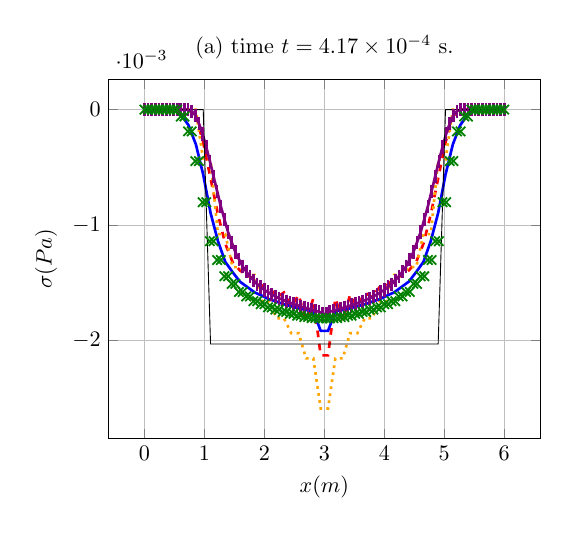
\begin{tikzpicture}[scale=0.8]
\begin{axis}[xlabel=$x (m)$,ylabel=$\sigma (Pa)$,ymajorgrids=true,xmajorgrids=true,legend pos=outer north east,title={(a) time $t = 4.17\times 10^{-4} $ s.}]
\addplot[Red,very thick,mark=none,dashed,mark size=3pt] coordinates {(0.0,0.0) (0.12244897959183673,0.0) (0.24489795918367346,0.0) (0.36734693877551017,0.0) (0.4897959183673469,0.0) (0.6122448979591837,0.0) (0.7346938775510203,-2.4706782429363735e-08) (0.8571428571428571,-5.867248412773822e-05) (0.9795918367346939,-0.0002853985909009103) (1.1020408163265305,-0.0005954308472358931) (1.2244897959183674,-0.0009067525645628951) (1.346938775510204,-0.0011607638587132671) (1.4693877551020407,-0.0013217065077757637) (1.5918367346938775,-0.001393523421223813) (1.7142857142857142,-0.0014402781682397202) (1.836734693877551,-0.001461552187294357) (1.9591836734693877,-0.0015250051575437162) (2.0816326530612246,-0.0015397083451698904) (2.204081632653061,-0.0016263965881897985) (2.326530612244898,-0.001584700145509203) (2.4489795918367347,-0.0017078111584935985) (2.571428571428571,-0.0016048877218035973) (2.693877551020408,-0.0018328835327606574) (2.816326530612245,-0.0016358851522103) (2.9387755102040813,-0.0021294274804773317) (3.061224489795918,-0.002129426547597653) (3.183673469387755,-0.0016358852194835601) (3.306122448979592,-0.0018328832921382582) (3.4285714285714284,-0.001604886057347882) (3.5510204081632653,-0.0017078117058325802) (3.673469387755102,-0.0015847007508890318) (3.7959183673469385,-0.0016263971582342353) (3.9183673469387754,-0.0015397084813633913) (4.040816326530612,-0.0015250053001396053) (4.163265306122449,-0.0014615511159168702) (4.285714285714286,-0.0014402781807440878) (4.408163265306122,-0.0013935236806247933) (4.530612244897959,-0.001321706579770408) (4.653061224489796,-0.0011607638047327214) (4.775510204081632,-0.0009067523623300537) (4.8979591836734695,-0.0005954315608474032) (5.020408163265306,-0.00028539897431746516) (5.142857142857142,-5.8672396327078764e-05) (5.26530612244898,-2.4706615951376558e-08) (5.387755102040816,0.0) (5.5102040816326525,0.0) (5.63265306122449,0.0) (5.755102040816326,0.0) (5.877551020408163,0.0) (6.0,0.0) };
\addplot[Orange,very thick,mark=none,dotted,mark size=3pt] coordinates {(0.0,0.0) (0.12244897959183673,0.0) (0.24489795918367346,0.0) (0.36734693877551017,0.0) (0.4897959183673469,0.0) (0.6122448979591837,0.0) (0.7346938775510203,-1.3329387423615422e-06) (0.8571428571428571,-1.3329399682741624e-06) (0.9795918367346939,-0.0004338120793096049) (1.1020408163265305,-0.00043381217614808966) (1.2244897959183674,-0.001078652776713751) (1.346938775510204,-0.0010786535293541098) (1.4693877551020407,-0.0013650099887886696) (1.5918367346938775,-0.0013650113404006328) (1.7142857142857142,-0.0014329121375811849) (1.836734693877551,-0.0014329136944043039) (1.9591836734693877,-0.0016624890765427765) (2.0816326530612246,-0.0016624896584601775) (2.204081632653061,-0.0018093716904116442) (2.326530612244898,-0.0018093557849666007) (2.4489795918367347,-0.001937275181781511) (2.571428571428571,-0.0019372767907533067) (2.693877551020408,-0.002155642178534488) (2.816326530612245,-0.002155640662975193) (2.9387755102040813,-0.002589762284338859) (3.061224489795918,-0.002589762175847431) (3.183673469387755,-0.002155641790343871) (3.306122448979592,-0.0021556425157575805) (3.4285714285714284,-0.0019372793251291578) (3.5510204081632653,-0.0019372778636785944) (3.673469387755102,-0.001809371471616459) (3.7959183673469385,-0.0018093710487213093) (3.9183673469387754,-0.0016624882379853954) (4.040816326530612,-0.0016624885719197634) (4.163265306122449,-0.0014329097917241942) (4.285714285714286,-0.0014329117775789128) (4.408163265306122,-0.0013650088316187207) (4.530612244897959,-0.001365009042422446) (4.653061224489796,-0.001078652980021462) (4.775510204081632,-0.001078652849949022) (4.8979591836734695,-0.00043381214864893664) (5.020408163265306,-0.0004338120674484783) (5.142857142857142,-1.3329395376771903e-06) (5.26530612244898,-1.332938627165289e-06) (5.387755102040816,0.0) (5.5102040816326525,0.0) (5.63265306122449,0.0) (5.755102040816326,0.0) (5.877551020408163,0.0) (6.0,0.0) };
\addplot[Blue,very thick,mark=none,solid,mark size=3pt] coordinates {(0.0,0.0) (0.12244897959183673,0.0) (0.24489795918367346,0.0) (0.36734693877551017,0.0) (0.4897959183673469,0.0) (0.6122448979591837,-4.674064137054689e-05) (0.7346938775510203,-0.00013518141641477002) (0.8571428571428571,-0.0003011735782562717) (0.9795918367346939,-0.0005636191184290303) (1.1020408163265305,-0.0008947918749973022) (1.2244897959183674,-0.0011384428542662672) (1.346938775510204,-0.0013187180973942406) (1.4693877551020407,-0.001408189281014569) (1.5918367346938775,-0.0014907417101391338) (1.7142857142857142,-0.001537189060000376) (1.836734693877551,-0.0015836563418978444) (1.9591836734693877,-0.0016130039487940052) (2.0816326530612246,-0.0016435577731461581) (2.204081632653061,-0.0016642561995700664) (2.326530612244898,-0.0016867439942769163) (2.4489795918367347,-0.001703774730043751) (2.571428571428571,-0.0017222255334447718) (2.693877551020408,-0.0017362714731070671) (2.816326530612245,-0.0017483096006135576) (2.9387755102040813,-0.0019170417268551047) (3.061224489795918,-0.0019170417268550973) (3.183673469387755,-0.0017483096006135571) (3.306122448979592,-0.0017362714731070667) (3.4285714285714284,-0.0017222255334447718) (3.5510204081632653,-0.001703774730043751) (3.673469387755102,-0.001686743994276917) (3.7959183673469385,-0.0016642561995700667) (3.9183673469387754,-0.0016435577731461586) (4.040816326530612,-0.001613003948794007) (4.163265306122449,-0.001583656341897845) (4.285714285714286,-0.0015371890600003768) (4.408163265306122,-0.0014907417101391342) (4.530612244897959,-0.001408189281014569) (4.653061224489796,-0.001318718097394241) (4.775510204081632,-0.0011384428542662657) (4.8979591836734695,-0.000894791874997302) (5.020408163265306,-0.0005636191184290323) (5.142857142857142,-0.00030117357825627236) (5.26530612244898,-0.0001351814164147703) (5.387755102040816,-4.674064137054787e-05) (5.5102040816326525,0.0) (5.63265306122449,0.0) (5.755102040816326,0.0) (5.877551020408163,0.0) (6.0,0.0) };
\addplot[Purple,very thick,mark=|,solid,mark size=3pt] coordinates {(0.0,0.0) (0.06060606060606061,0.0) (0.12121212121212122,0.0) (0.18181818181818182,0.0) (0.24242424242424243,0.0) (0.30303030303030304,0.0) (0.36363636363636365,0.0) (0.42424242424242425,0.0) (0.48484848484848486,0.0) (0.5454545454545454,0.0) (0.6060606060606061,0.0) (0.6666666666666667,-4.0531023418027623e-11) (0.7272727272727273,-9.569933907036341e-07) (0.7878787878787878,-1.343261689597016e-05) (0.8484848484848485,-4.9558531577573574e-05) (0.9090909090909092,-0.00012085333050559284) (0.9696969696969697,-0.00021200690708122615) (1.0303030303030303,-0.0003243493959749349) (1.0909090909090908,-0.0004471679110108456) (1.1515151515151516,-0.0005777044805089968) (1.2121212121212122,-0.0007079212371215294) (1.2727272727272727,-0.0008366965691899573) (1.3333333333333335,-0.0009513341656497712) (1.393939393939394,-0.0010611178168264638) (1.4545454545454546,-0.0011492229400598727) (1.5151515151515151,-0.0012334657955739342) (1.5757575757575757,-0.0012964181089512702) (1.6363636363636365,-0.0013579641179089666) (1.696969696969697,-0.0014023349566352568) (1.7575757575757576,-0.0014472561599906432) (1.8181818181818183,-0.0014792542904296902) (1.878787878787879,-0.0015129085145436797) (1.9393939393939394,-0.001536820399711865) (2.0,-0.0015629352013383615) (2.0606060606060606,-0.001581443333690898) (2.121212121212121,-0.0016024369422373745) (2.1818181818181817,-0.0016172073793473665) (2.2424242424242427,-0.0016346556959052913) (2.303030303030303,-0.0016467496593637076) (2.3636363636363638,-0.0016617233860291073) (2.4242424242424243,-0.0016718388130052982) (2.484848484848485,-0.0016851233861680903) (2.5454545454545454,-0.0016937313987460364) (2.606060606060606,-0.0017059907853383823) (2.666666666666667,-0.0017134098017108522) (2.7272727272727275,-0.0017253826926178872) (2.787878787878788,-0.0017318058838217147) (2.8484848484848486,-0.0017448175639310159) (2.909090909090909,-0.00175019771707795) (2.9696969696969697,-0.0017717316670483852) (3.0303030303030303,-0.0017717316670483854) (3.090909090909091,-0.00175019771707795) (3.1515151515151514,-0.0017448175639310163) (3.2121212121212124,-0.001731805883821715) (3.272727272727273,-0.0017253826926178879) (3.3333333333333335,-0.001713409801710852) (3.393939393939394,-0.0017059907853383828) (3.4545454545454546,-0.001693731398746037) (3.515151515151515,-0.001685123386168091) (3.5757575757575757,-0.0016718388130052986) (3.6363636363636367,-0.0016617233860291081) (3.6969696969696972,-0.001646749659363708) (3.757575757575758,-0.001634655695905292) (3.8181818181818183,-0.0016172073793473672) (3.878787878787879,-0.0016024369422373756) (3.9393939393939394,-0.001581443333690899) (4.0,-0.0015629352013383628) (4.0606060606060606,-0.0015368203997118664) (4.121212121212121,-0.0015129085145436816) (4.181818181818182,-0.0014792542904296917) (4.242424242424242,-0.001447256159990645) (4.303030303030303,-0.0014023349566352596) (4.363636363636363,-0.00135796411790897) (4.424242424242425,-0.0012964181089512726) (4.484848484848485,-0.001233465795573936) (4.545454545454546,-0.0011492229400598753) (4.606060606060606,-0.0010611178168264672) (4.666666666666667,-0.0009513341656497752) (4.7272727272727275,-0.000836696569189961) (4.787878787878788,-0.0007079212371215326) (4.848484848484849,-0.0005777044805089981) (4.909090909090909,-0.00044716791101084754) (4.96969696969697,-0.00032434939597493647) (5.03030303030303,-0.0002120069070812274) (5.090909090909091,-0.00012085333050559367) (5.151515151515151,-4.955853157757462e-05) (5.212121212121212,-1.3432616895970462e-05) (5.2727272727272725,-9.56993390703686e-07) (5.333333333333334,-4.0531023418038635e-11) (5.3939393939393945,0.0) (5.454545454545455,0.0) (5.515151515151516,0.0) (5.575757575757576,0.0) (5.636363636363637,0.0) (5.696969696969697,0.0) (5.757575757575758,0.0) (5.818181818181818,0.0) (5.878787878787879,0.0) (5.9393939393939394,0.0) (6.0,0.0) };
\addplot[Green,thick,mark=x,only marks,mark size=3pt] coordinates {(0.0,0.0) (0.06060606060606061,0.0) (0.12121212121212122,0.0) (0.18181818181818182,0.0) (0.24242424242424243,0.0) (0.30303030303030304,0.0) (0.36363636363636365,0.0) (0.42424242424242425,0.0) (0.48484848484848486,0.0) (0.5454545454545454,0.0) (0.6060606060606061,-5.95994308592662e-05) (0.6666666666666667,-5.959943085926653e-05) (0.7272727272727273,-0.00018884662936873652) (0.7878787878787878,-0.00018884662936873706) (0.8484848484848485,-0.0004463332330303008) (0.9090909090909092,-0.00044633323303030104) (0.9696969696969697,-0.0008024468949020794) (1.0303030303030303,-0.0008024468949020728) (1.0909090909090908,-0.0011402025229616407) (1.1515151515151516,-0.0011402025229616413) (1.2121212121212122,-0.001303374963621311) (1.2727272727272727,-0.0013033749636213118) (1.3333333333333335,-0.0014435674663425906) (1.393939393939394,-0.0014435674663425915) (1.4545454545454546,-0.0015100315038270278) (1.5151515151515151,-0.0015100315038270632) (1.5757575757575757,-0.0015802302171187615) (1.6363636363636365,-0.0015802302171187552) (1.696969696969697,-0.0016188693449786943) (1.7575757575757576,-0.0016188693449786839) (1.8181818181818183,-0.0016602445166918156) (1.878787878787879,-0.0016602445166918167) (1.9393939393939394,-0.0016861774822787279) (2.0,-0.0016861774822787287) (2.0606060606060606,-0.0017138047010635522) (2.121212121212121,-0.0017138047010635828) (2.1818181818181817,-0.001733009016979971) (2.2424242424242427,-0.001733009016980024) (2.303030303030303,-0.0017535801619425328) (2.3636363636363638,-0.0017535801619425221) (2.4242424242424243,-0.0017693554459473537) (2.484848484848485,-0.001769355445947317) (2.5454545454545454,-0.0017856035728642274) (2.606060606060606,-0.0017856035728642042) (2.666666666666667,-0.0017976908098995877) (2.7272727272727275,-0.0017976908098995808) (2.787878787878788,-0.001806107529340324) (2.8484848484848486,-0.001806107529340337) (2.909090909090909,-0.0018091152724179298) (2.9696969696969697,-0.0018091152724178296) (3.0303030303030303,-0.001809115272417879) (3.090909090909091,-0.001809115272417851) (3.1515151515151514,-0.0018061075293403382) (3.2121212121212124,-0.0018061075293403603) (3.272727272727273,-0.0017976908098994923) (3.3333333333333335,-0.0017976908098994875) (3.393939393939394,-0.0017856035728641474) (3.4545454545454546,-0.0017856035728641513) (3.515151515151515,-0.0017693554459472887) (3.5757575757575757,-0.0017693554459472952) (3.6363636363636367,-0.0017535801619425245) (3.6969696969696972,-0.0017535801619425078) (3.757575757575758,-0.0017330090169799064) (3.8181818181818183,-0.0017330090169799365) (3.878787878787879,-0.0017138047010635275) (3.9393939393939394,-0.0017138047010634284) (4.0,-0.0016861774822786698) (4.0606060606060606,-0.0016861774822786624) (4.121212121212121,-0.0016602445166917154) (4.181818181818182,-0.0016602445166917187) (4.242424242424242,-0.0016188693449785446) (4.303030303030303,-0.0016188693449785436) (4.363636363636363,-0.001580230217118671) (4.424242424242425,-0.0015802302171186698) (4.484848484848485,-0.0015100315038270133) (4.545454545454546,-0.0015100315038270502) (4.606060606060606,-0.0014435674663425381) (4.666666666666667,-0.0014435674663425414) (4.7272727272727275,-0.0013033749636212864) (4.787878787878788,-0.0013033749636212884) (4.848484848484849,-0.0011402025229617428) (4.909090909090909,-0.0011402025229617456) (4.96969696969697,-0.0008024468949021485) (5.03030303030303,-0.0008024468949021475) (5.090909090909091,-0.000446333233030326) (5.151515151515151,-0.0004463332330303249) (5.212121212121212,-0.00018884662936874592) (5.2727272727272725,-0.00018884662936874598) (5.333333333333334,-5.95994308592702e-05) (5.3939393939393945,-5.959943085927111e-05) (5.454545454545455,0.0) (5.515151515151516,0.0) (5.575757575757576,0.0) (5.636363636363637,0.0) (5.696969696969697,0.0) (5.757575757575758,0.0) (5.818181818181818,0.0) (5.878787878787879,0.0) (5.9393939393939394,0.0) (6.0,0.0) };
\addplot[black,thin,mark=none,solid,mark size=3pt] coordinates {(0.0,-0.0) (0.12244897959183673,-0.0) (0.24489795918367346,-0.0) (0.36734693877551017,-0.0) (0.4897959183673469,-0.0) (0.6122448979591837,-0.0) (0.7346938775510203,-0.0) (0.8571428571428571,-0.0) (0.9795918367346939,-0.0) (1.1020408163265305,-0.002030785796418313) (1.2244897959183674,-0.002030785796418313) (1.346938775510204,-0.002030785796418313) (1.4693877551020407,-0.002030785796418313) (1.5918367346938775,-0.002030785796418313) (1.7142857142857142,-0.002030785796418313) (1.836734693877551,-0.002030785796418313) (1.9591836734693877,-0.002030785796418313) (2.0816326530612246,-0.002030785796418313) (2.204081632653061,-0.002030785796418313) (2.326530612244898,-0.002030785796418313) (2.4489795918367347,-0.002030785796418313) (2.571428571428571,-0.002030785796418313) (2.693877551020408,-0.002030785796418313) (2.816326530612245,-0.002030785796418313) (2.9387755102040813,-0.002030785796418313) (3.061224489795918,-0.002030785796418313) (3.183673469387755,-0.002030785796418313) (3.306122448979592,-0.002030785796418313) (3.4285714285714284,-0.002030785796418313) (3.5510204081632653,-0.002030785796418313) (3.673469387755102,-0.002030785796418313) (3.7959183673469385,-0.002030785796418313) (3.9183673469387754,-0.002030785796418313) (4.040816326530612,-0.002030785796418313) (4.163265306122449,-0.002030785796418313) (4.285714285714286,-0.002030785796418313) (4.408163265306122,-0.002030785796418313) (4.530612244897959,-0.002030785796418313) (4.653061224489796,-0.002030785796418313) (4.775510204081632,-0.002030785796418313) (4.8979591836734695,-0.002030785796418313) (5.020408163265306,-0.0) (5.142857142857142,-0.0) (5.26530612244898,-0.0) (5.387755102040816,-0.0) (5.5102040816326525,-0.0) (5.63265306122449,-0.0) (5.755102040816326,-0.0) (5.877551020408163,-0.0) (6.0,-0.0) };
%\legend{usl 1ppc,usf 1ppc,dgmpm 1ppc,dgmpm 2ppc,dgmpm 2ppc (RK2 + strang),plastic solution}
\end{axis}
\end{tikzpicture}
%%% Local Variables:
%%% mode: latex
%%% TeX-master: "../../mainManuscript"
%%% End:
}
%   {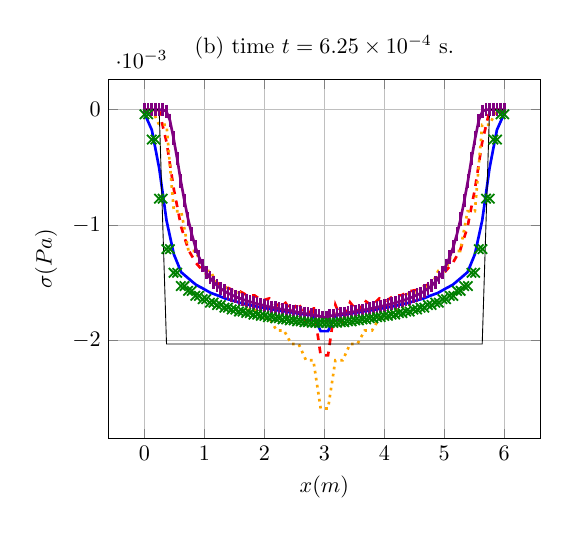
\begin{tikzpicture}[scale=0.8]
\begin{axis}[xlabel=$x (m)$,ylabel=$\sigma (Pa)$,ymajorgrids=true,xmajorgrids=true,legend pos=outer north east,title={(b) time $t = 6.25\times 10^{-4} $ s.}]
\addplot[Red,very thick,mark=none,dashed,mark size=3pt] coordinates {(0.0,0.0) (0.12244897959183673,0.0) (0.24489795918367346,-9.09743714498828e-06) (0.36734693877551017,-0.00028060178384402246) (0.4897959183673469,-0.000690645014524663) (0.6122448979591837,-0.0010172754869474821) (0.7346938775510203,-0.0012174879404668873) (0.8571428571428571,-0.001327790359856718) (0.9795918367346939,-0.0014002058405938708) (1.1020408163265305,-0.0014574762656029724) (1.2244897959183674,-0.001505353831791513) (1.346938775510204,-0.0015338005451529275) (1.4693877551020407,-0.0015635221192807454) (1.5918367346938775,-0.0015753991257001431) (1.7142857142857142,-0.0016098352308080907) (1.836734693877551,-0.0016105966109038212) (1.9591836734693877,-0.0016554023072314432) (2.0816326530612246,-0.0016360935152320186) (2.204081632653061,-0.0016986137246127954) (2.326530612244898,-0.0016550171076523833) (2.4489795918367347,-0.0017506128422217714) (2.571428571428571,-0.001670222601515723) (2.693877551020408,-0.001843959044053449) (2.816326530612245,-0.0016915571845227079) (2.9387755102040813,-0.002129427489038802) (3.061224489795918,-0.0021294265561618607) (3.183673469387755,-0.0016915572429560084) (3.306122448979592,-0.0018439587286891077) (3.4285714285714284,-0.0016702218101354916) (3.5510204081632653,-0.001750613256004356) (3.673469387755102,-0.0016550174088773542) (3.7959183673469385,-0.001698614023304057) (3.9183673469387754,-0.0016360936167129818) (4.040816326530612,-0.0016554021914399486) (4.163265306122449,-0.0016105964191050952) (4.285714285714286,-0.0016098352679559734) (4.408163265306122,-0.0015753992486767384) (4.530612244897959,-0.0015635221977266104) (4.653061224489796,-0.0015338005571043653) (4.775510204081632,-0.0015053538409978895) (4.8979591836734695,-0.001457476331976043) (5.020408163265306,-0.001400205486223803) (5.142857142857142,-0.0013277905131784619) (5.26530612244898,-0.0012174886002592263) (5.387755102040816,-0.0010172757767319969) (5.5102040816326525,-0.0006906448932635886) (5.63265306122449,-0.0002806022282810553) (5.755102040816326,-9.097387796699236e-06) (5.877551020408163,0.0) (6.0,0.0) };
\addplot[Orange,very thick,mark=none,dotted,mark size=3pt] coordinates {(0.0,0.0) (0.12244897959183673,0.0) (0.24489795918367346,-0.00013125567272782819) (0.36734693877551017,-0.00013125591615145197) (0.4897959183673469,-0.0008813832603320562) (0.6122448979591837,-0.0008813838642660081) (0.7346938775510203,-0.0012247428359422696) (0.8571428571428571,-0.0012247425724953693) (0.9795918367346939,-0.001397689841428779) (1.1020408163265305,-0.0013976897509958288) (1.2244897959183674,-0.001536227538045054) (1.346938775510204,-0.001536227937408319) (1.4693877551020407,-0.0015850329963259663) (1.5918367346938775,-0.0015850318594526924) (1.7142857142857142,-0.0017348225074951447) (1.836734693877551,-0.0017348212862825618) (1.9591836734693877,-0.0018063592675864129) (2.0816326530612246,-0.001806359731310172) (2.204081632653061,-0.0019134829069542122) (2.326530612244898,-0.0019134752699114365) (2.4489795918367347,-0.0020308300009669426) (2.571428571428571,-0.0020308316942653946) (2.693877551020408,-0.0021721534919969363) (2.816326530612245,-0.0021721522612295503) (2.9387755102040813,-0.002589832926025744) (3.061224489795918,-0.0025898328149225646) (3.183673469387755,-0.002172153099923732) (3.306122448979592,-0.002172153496185014) (3.4285714285714284,-0.0020308319106928136) (3.5510204081632653,-0.002030831353584487) (3.673469387755102,-0.0019134829101521314) (3.7959183673469385,-0.0019134826107273153) (3.9183673469387754,-0.0018063586181389377) (4.040816326530612,-0.0018063592789159533) (4.163265306122449,-0.001734821842983902) (4.285714285714286,-0.0017348222168737536) (4.408163265306122,-0.0015850322909855233) (4.530612244897959,-0.0015850322551182372) (4.653061224489796,-0.0015362286519360463) (4.775510204081632,-0.0015362274905299917) (4.8979591836734695,-0.0013976888757025222) (5.020408163265306,-0.0013976898142422994) (5.142857142857142,-0.0012247427216731783) (5.26530612244898,-0.0012247427719878296) (5.387755102040816,-0.0008813837524078346) (5.5102040816326525,-0.000881379580518873) (5.63265306122449,-0.00013125562655680082) (5.755102040816326,-0.0001312556126026732) (5.877551020408163,0.0) (6.0,0.0) };
\addplot[Blue,very thick,mark=none,solid,mark size=3pt] coordinates {(0.0,-3.288656606774586e-05) (0.12244897959183673,-0.00017641909201459894) (0.24489795918367346,-0.000506646129358451) (0.36734693877551017,-0.0009600605637646077) (0.4897959183673469,-0.001253427110389605) (0.6122448979591837,-0.0014089288532961235) (0.7346938775510203,-0.0014636954486616234) (0.8571428571428571,-0.0015173032590703268) (0.9795918367346939,-0.001551337471828278) (1.1020408163265305,-0.0015875427344901954) (1.2244897959183674,-0.0016109960299248184) (1.346938775510204,-0.0016369488867646299) (1.4693877551020407,-0.0016544898328871023) (1.5918367346938775,-0.0016739161084835994) (1.7142857142857142,-0.001687923915138772) (1.836734693877551,-0.0017030619275038906) (1.9591836734693877,-0.0017147494357043645) (2.0816326530612246,-0.0017269459689745993) (2.204081632653061,-0.0017370154541442267) (2.326530612244898,-0.001747456536468629) (2.4489795918367347,-0.0017569942648830645) (2.571428571428571,-0.0017669191588267057) (2.693877551020408,-0.0017756679773472232) (2.816326530612245,-0.0017829750209496743) (2.9387755102040813,-0.0019198249761128202) (3.061224489795918,-0.001919824976112813) (3.183673469387755,-0.001782975020949674) (3.306122448979592,-0.0017756679773472232) (3.4285714285714284,-0.001766919158826706) (3.5510204081632653,-0.0017569942648830654) (3.673469387755102,-0.0017474565364686298) (3.7959183673469385,-0.0017370154541442278) (3.9183673469387754,-0.0017269459689746) (4.040816326530612,-0.0017147494357043658) (4.163265306122449,-0.0017030619275038915) (4.285714285714286,-0.0016879239151387725) (4.408163265306122,-0.0016739161084836) (4.530612244897959,-0.0016544898328871031) (4.653061224489796,-0.001636948886764631) (4.775510204081632,-0.0016109960299248193) (4.8979591836734695,-0.001587542734490196) (5.020408163265306,-0.0015513374718282788) (5.142857142857142,-0.0015173032590703277) (5.26530612244898,-0.0014636954486616236) (5.387755102040816,-0.0014089288532961226) (5.5102040816326525,-0.0012534271103896038) (5.63265306122449,-0.000960060563764606) (5.755102040816326,-0.0005066461293584512) (5.877551020408163,-0.00017641909201459888) (6.0,-3.2886566067745944e-05) };
\addplot[Purple,very thick,mark=|,solid,mark size=3pt] coordinates {(0.0,0.0) (0.06060606060606061,0.0) (0.12121212121212122,0.0) (0.18181818181818182,0.0) (0.24242424242424243,0.0) (0.30303030303030304,-1.192012716404481e-07) (0.36363636363636365,-1.4562449689300448e-05) (0.42424242424242425,-9.236457975705467e-05) (0.48484848484848486,-0.0002470376030914057) (0.5454545454545454,-0.000425718225432667) (0.6060606060606061,-0.0006194023809233477) (0.6666666666666667,-0.0007903226149766369) (0.7272727272727273,-0.0009484637233093347) (0.7878787878787878,-0.001077982039857484) (0.8484848484848485,-0.0011884743153909919) (0.9090909090909092,-0.001277319324857129) (0.9696969696969697,-0.0013502507843687374) (1.0303030303030303,-0.0014093248881660956) (1.0909090909090908,-0.001456586468333663) (1.1515151515151516,-0.0014954551893398439) (1.2121212121212122,-0.0015258020679790962) (1.2727272727272727,-0.0015519977804941763) (1.3333333333333335,-0.0015722461442494063) (1.393939393939394,-0.0015911837536253385) (1.4545454545454546,-0.0016058566241831974) (1.5151515151515151,-0.0016207034860120757) (1.5757575757575757,-0.0016322577806829907) (1.6363636363636365,-0.0016446308515186924) (1.696969696969697,-0.0016542659958777353) (1.7575757575757576,-0.0016649744154638819) (1.8181818181818183,-0.0016732800734457133) (1.878787878787879,-0.0016827672710207039) (1.9393939393939394,-0.0016900659440740899) (2.0,-0.0016986145006445332) (2.0606060606060606,-0.0017051104495914072) (2.121212121212121,-0.0017129279540977528) (2.1818181818181817,-0.0017187667900267708) (2.2424242424242427,-0.0017260236649975474) (2.303030303030303,-0.0017313165739623365) (2.3636363636363638,-0.0017381681294236975) (2.4242424242424243,-0.0017430027538714655) (2.484848484848485,-0.0017496107790071042) (2.5454545454545454,-0.0017540562886207848) (2.606060606060606,-0.0017606250777175883) (2.666666666666667,-0.0017647324970514386) (2.7272727272727275,-0.0017715990863667725) (2.787878787878788,-0.0017753916177228703) (2.8484848484848486,-0.0017833572523661626) (2.909090909090909,-0.0017867388502595498) (2.9696969696969697,-0.0018009642034702022) (3.0303030303030303,-0.0018009642034702024) (3.090909090909091,-0.0017867388502595498) (3.1515151515151514,-0.0017833572523661633) (3.2121212121212124,-0.0017753916177228705) (3.272727272727273,-0.0017715990863667731) (3.3333333333333335,-0.0017647324970514388) (3.393939393939394,-0.0017606250777175893) (3.4545454545454546,-0.0017540562886207858) (3.515151515151515,-0.0017496107790071053) (3.5757575757575757,-0.0017430027538714663) (3.6363636363636367,-0.0017381681294236994) (3.6969696969696972,-0.0017313165739623376) (3.757575757575758,-0.0017260236649975485) (3.8181818181818183,-0.0017187667900267715) (3.878787878787879,-0.0017129279540977545) (3.9393939393939394,-0.0017051104495914087) (4.0,-0.0016986145006445343) (4.0606060606060606,-0.0016900659440740914) (4.121212121212121,-0.0016827672710207056) (4.181818181818182,-0.001673280073445715) (4.242424242424242,-0.0016649744154638838) (4.303030303030303,-0.0016542659958777375) (4.363636363636363,-0.0016446308515186954) (4.424242424242425,-0.0016322577806829933) (4.484848484848485,-0.0016207034860120783) (4.545454545454546,-0.0016058566241832003) (4.606060606060606,-0.001591183753625341) (4.666666666666667,-0.0015722461442494097) (4.7272727272727275,-0.001551997780494179) (4.787878787878788,-0.0015258020679791) (4.848484848484849,-0.0014954551893398465) (4.909090909090909,-0.0014565864683336663) (4.96969696969697,-0.0014093248881660982) (5.03030303030303,-0.0013502507843687402) (5.090909090909091,-0.0012773193248571315) (5.151515151515151,-0.001188474315390994) (5.212121212121212,-0.001077982039857487) (5.2727272727272725,-0.0009484637233093383) (5.333333333333334,-0.0007903226149766394) (5.3939393939393945,-0.0006194023809233497) (5.454545454545455,-0.00042571822543266863) (5.515151515151516,-0.000247037603091407) (5.575757575757576,-9.236457975705492e-05) (5.636363636363637,-1.4562449689300525e-05) (5.696969696969697,-1.1920127164044906e-07) (5.757575757575758,0.0) (5.818181818181818,0.0) (5.878787878787879,0.0) (5.9393939393939394,0.0) (6.0,0.0) };
\addplot[Green,thick,mark=x,only marks,mark size=3pt] coordinates {(0.0,-4.077076000132571e-05) (0.06060606060606061,-4.077076000132737e-05) (0.12121212121212122,-0.000259465833593339) (0.18181818181818182,-0.0002594658335933402) (0.24242424242424243,-0.0007718131581974564) (0.30303030303030304,-0.0007718131581974544) (0.36363636363636365,-0.0012089832811266732) (0.42424242424242425,-0.0012089832811266726) (0.48484848484848486,-0.0014141342215499664) (0.5454545454545454,-0.001414134221549973) (0.6060606060606061,-0.0015288994593393016) (0.6666666666666667,-0.0015288994593392992) (0.7272727272727273,-0.001570800224198939) (0.7878787878787878,-0.0015708002241989342) (0.8484848484848485,-0.0016141244026557006) (0.9090909090909092,-0.0016141244026557173) (0.9696969696969697,-0.0016423561224507385) (1.0303030303030303,-0.0016423561224507043) (1.0909090909090908,-0.0016729153381830181) (1.1515151515151516,-0.0016729153381830314) (1.2121212121212122,-0.0016934523002053714) (1.2727272727272727,-0.0016934523002054237) (1.3333333333333335,-0.001716262292786097) (1.393939393939394,-0.0017162622927860622) (1.4545454545454546,-0.0017321137630453758) (1.5151515151515151,-0.0017321137630453532) (1.5757575757575757,-0.0017497799126621094) (1.6363636363636365,-0.0017497799126621125) (1.696969696969697,-0.0017625571698028399) (1.7575757575757576,-0.0017625571698028355) (1.8181818181818183,-0.001776558904084057) (1.878787878787879,-0.0017765589040840486) (1.9393939393939394,-0.0017871695859244035) (2.0,-0.0017871695859243287) (2.0606060606060606,-0.0017985263217785796) (2.121212121212121,-0.0017985263217786393) (2.1818181818181817,-0.0018077111881619988) (2.2424242424242427,-0.0018077111881619735) (2.303030303030303,-0.0018174288517170986) (2.3636363636363638,-0.0018174288517171257) (2.4242424242424243,-0.0018259390176408893) (2.484848484848485,-0.0018259390176408438) (2.5454545454545454,-0.001834601910130878) (2.606060606060606,-0.00183460191013079) (2.666666666666667,-0.0018417911948099834) (2.7272727272727275,-0.0018417911948099739) (2.787878787878788,-0.0018466992729078942) (2.8484848484848486,-0.001846699272907896) (2.909090909090909,-0.0018486141474135926) (2.9696969696969697,-0.001848614147413537) (3.0303030303030303,-0.001848614147413566) (3.090909090909091,-0.0018486141474135737) (3.1515151515151514,-0.001846699272907917) (3.2121212121212124,-0.001846699272907892) (3.272727272727273,-0.0018417911948100014) (3.3333333333333335,-0.0018417911948099752) (3.393939393939394,-0.001834601910130857) (3.4545454545454546,-0.0018346019101308337) (3.515151515151515,-0.0018259390176409316) (3.5757575757575757,-0.001825939017640955) (3.6363636363636367,-0.0018174288517171517) (3.6969696969696972,-0.0018174288517170893) (3.757575757575758,-0.001807711188161973) (3.8181818181818183,-0.0018077111881620055) (3.878787878787879,-0.001798526321778638) (3.9393939393939394,-0.001798526321778626) (4.0,-0.001787169585924375) (4.0606060606060606,-0.0017871695859243203) (4.121212121212121,-0.0017765589040840638) (4.181818181818182,-0.0017765589040839964) (4.242424242424242,-0.0017625571698028266) (4.303030303030303,-0.0017625571698028134) (4.363636363636363,-0.0017497799126621459) (4.424242424242425,-0.001749779912662138) (4.484848484848485,-0.0017321137630453144) (4.545454545454546,-0.0017321137630453304) (4.606060606060606,-0.0017162622927860659) (4.666666666666667,-0.0017162622927860381) (4.7272727272727275,-0.0016934523002054068) (4.787878787878788,-0.0016934523002054246) (4.848484848484849,-0.0016729153381829882) (4.909090909090909,-0.001672915338182986) (4.96969696969697,-0.001642356122450608) (5.03030303030303,-0.001642356122450549) (5.090909090909091,-0.0016141244026555914) (5.151515151515151,-0.001614124402655621) (5.212121212121212,-0.0015708002241988284) (5.2727272727272725,-0.0015708002241988448) (5.333333333333334,-0.0015288994593392303) (5.3939393939393945,-0.001528899459339235) (5.454545454545455,-0.0014141342215499202) (5.515151515151516,-0.001414134221549916) (5.575757575757576,-0.0012089832811266546) (5.636363636363637,-0.001208983281126654) (5.696969696969697,-0.000771813158197516) (5.757575757575758,-0.000771813158197514) (5.818181818181818,-0.0002594658335933476) (5.878787878787879,-0.00025946583359334876) (5.9393939393939394,-4.0770760001336276e-05) (6.0,-4.077076000133824e-05) };
\addplot[black,thin,mark=none,solid,mark size=3pt] coordinates {(0.0,-0.0) (0.12244897959183673,-0.0) (0.24489795918367346,-0.0) (0.36734693877551017,-0.002030785796418313) (0.4897959183673469,-0.002030785796418313) (0.6122448979591837,-0.002030785796418313) (0.7346938775510203,-0.002030785796418313) (0.8571428571428571,-0.002030785796418313) (0.9795918367346939,-0.002030785796418313) (1.1020408163265305,-0.002030785796418313) (1.2244897959183674,-0.002030785796418313) (1.346938775510204,-0.002030785796418313) (1.4693877551020407,-0.002030785796418313) (1.5918367346938775,-0.002030785796418313) (1.7142857142857142,-0.002030785796418313) (1.836734693877551,-0.002030785796418313) (1.9591836734693877,-0.002030785796418313) (2.0816326530612246,-0.002030785796418313) (2.204081632653061,-0.002030785796418313) (2.326530612244898,-0.002030785796418313) (2.4489795918367347,-0.002030785796418313) (2.571428571428571,-0.002030785796418313) (2.693877551020408,-0.002030785796418313) (2.816326530612245,-0.002030785796418313) (2.9387755102040813,-0.002030785796418313) (3.061224489795918,-0.002030785796418313) (3.183673469387755,-0.002030785796418313) (3.306122448979592,-0.002030785796418313) (3.4285714285714284,-0.002030785796418313) (3.5510204081632653,-0.002030785796418313) (3.673469387755102,-0.002030785796418313) (3.7959183673469385,-0.002030785796418313) (3.9183673469387754,-0.002030785796418313) (4.040816326530612,-0.002030785796418313) (4.163265306122449,-0.002030785796418313) (4.285714285714286,-0.002030785796418313) (4.408163265306122,-0.002030785796418313) (4.530612244897959,-0.002030785796418313) (4.653061224489796,-0.002030785796418313) (4.775510204081632,-0.002030785796418313) (4.8979591836734695,-0.002030785796418313) (5.020408163265306,-0.002030785796418313) (5.142857142857142,-0.002030785796418313) (5.26530612244898,-0.002030785796418313) (5.387755102040816,-0.002030785796418313) (5.5102040816326525,-0.002030785796418313) (5.63265306122449,-0.002030785796418313) (5.755102040816326,-0.0) (5.877551020408163,-0.0) (6.0,-0.0) };
%\legend{usl 1ppc,usf 1ppc,dgmpm 1ppc,dgmpm 2ppc,dgmpm 2ppc (RK2 + strang),plastic solution}
\end{axis}
\end{tikzpicture}
%%% Local Variables:
%%% mode: latex
%%% TeX-master: "../../mainManuscript"
%%% End:
}
%   {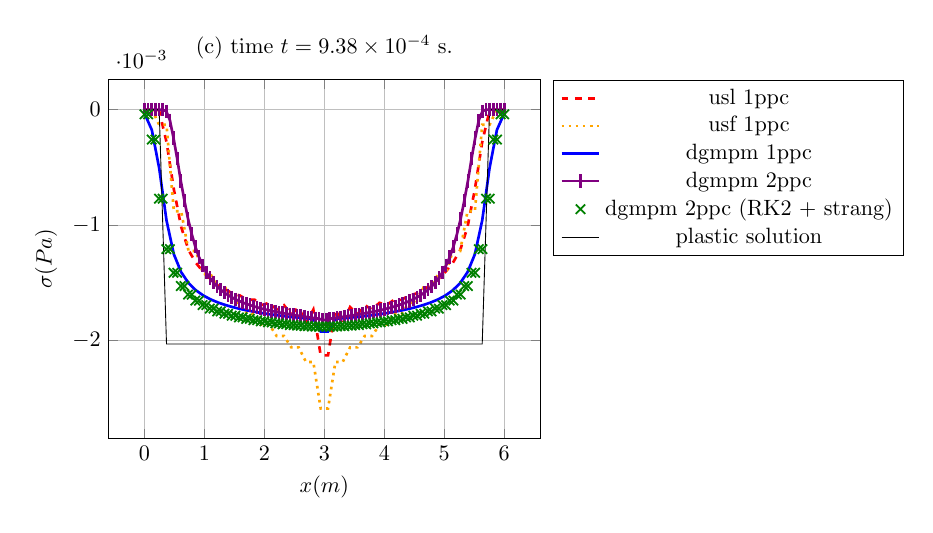
\begin{tikzpicture}[scale=0.8]
\begin{axis}[xlabel=$x (m)$,ylabel=$\sigma (Pa)$,ymajorgrids=true,xmajorgrids=true,legend pos=outer north east,title={(c) time $t = 9.38\times 10^{-4} $ s.}]
\addplot[Red,very thick,mark=none,dashed,mark size=3pt] coordinates {(0.0,0.0) (0.12244897959183673,0.0) (0.24489795918367346,-9.09743714498828e-06) (0.36734693877551017,-0.00028060178384402246) (0.4897959183673469,-0.000690645014524663) (0.6122448979591837,-0.0010172754869474821) (0.7346938775510203,-0.0012174879404668873) (0.8571428571428571,-0.0013280180462532844) (0.9795918367346939,-0.001405573314687709) (1.1020408163265305,-0.0014715381825829389) (1.2244897959183674,-0.0015240182188866489) (1.346938775510204,-0.0015561890073244227) (1.4693877551020407,-0.0015945318145481168) (1.5918367346938775,-0.0016110732006773488) (1.7142857142857142,-0.0016486349228612136) (1.836734693877551,-0.0016475965034896671) (1.9591836734693877,-0.0016928166346279892) (2.0816326530612246,-0.001674127735672926) (2.204081632653061,-0.0017324385481802082) (2.326530612244898,-0.0016946099760850012) (2.4489795918367347,-0.0017749462373902935) (2.571428571428571,-0.0017118415467530894) (2.693877551020408,-0.0018524608793206972) (2.816326530612245,-0.0017331235724179987) (2.9387755102040813,-0.0021294274890493736) (3.061224489795918,-0.0021294265561724456) (3.183673469387755,-0.0017331236195573326) (3.306122448979592,-0.001852460536357857) (3.4285714285714284,-0.0017118410940132381) (3.5510204081632653,-0.0017749465825430376) (3.673469387755102,-0.0016946101804939575) (3.7959183673469385,-0.0017324387664782147) (3.9183673469387754,-0.0016741278276934143) (4.040816326530612,-0.0016928165624296699) (4.163265306122449,-0.00164759638416514) (4.285714285714286,-0.0016486349315771296) (4.408163265306122,-0.0016110732691248558) (4.530612244897959,-0.0015945318680601172) (4.653061224489796,-0.001556189037305485) (4.775510204081632,-0.001524018258266158) (4.8979591836734695,-0.0014715382275786231) (5.020408163265306,-0.001405572961530602) (5.142857142857142,-0.0013280181972431424) (5.26530612244898,-0.0012174886002592263) (5.387755102040816,-0.0010172757767319969) (5.5102040816326525,-0.0006906448932635886) (5.63265306122449,-0.0002806022282810553) (5.755102040816326,-9.097387796699236e-06) (5.877551020408163,0.0) (6.0,0.0) };
\addplot[Orange,very thick,mark=none,dotted,mark size=3pt] coordinates {(0.0,0.0) (0.12244897959183673,0.0) (0.24489795918367346,-0.00013125567272782819) (0.36734693877551017,-0.00013125591615145197) (0.4897959183673469,-0.0008813832603320562) (0.6122448979591837,-0.0008813838642660081) (0.7346938775510203,-0.0012247851551192936) (0.8571428571428571,-0.001224784890440556) (0.9795918367346939,-0.0014249339778741803) (1.1020408163265305,-0.0014249341228939742) (1.2244897959183674,-0.0015414554008737465) (1.346938775510204,-0.0015414557554649711) (1.4693877551020407,-0.0016738699379305296) (1.5918367346938775,-0.0016738690962649337) (1.7142857142857142,-0.0017713609761048244) (1.836734693877551,-0.0017713599892547082) (1.9591836734693877,-0.0018625169761770728) (2.0816326530612246,-0.0018625172930377735) (2.204081632653061,-0.001961668570283414) (2.326530612244898,-0.0019616634232208813) (2.4489795918367347,-0.0020602990364256483) (2.571428571428571,-0.002060300428159983) (2.693877551020408,-0.0021870752843109642) (2.816326530612245,-0.002187074359760412) (2.9387755102040813,-0.0025898336000690844) (3.061224489795918,-0.002589833489024399) (3.183673469387755,-0.0021870749435822555) (3.306122448979592,-0.002187075320243097) (3.4285714285714284,-0.0020603004028730636) (3.5510204081632653,-0.002060299945635322) (3.673469387755102,-0.001961668579229524) (3.7959183673469385,-0.0019616680989035505) (3.9183673469387754,-0.0018625166965802594) (4.040816326530612,-0.0018625168203206587) (4.163265306122449,-0.0017713603337100934) (4.285714285714286,-0.0017713606793835414) (4.408163265306122,-0.0016738693883742992) (4.530612244897959,-0.0016738697730550773) (4.653061224489796,-0.0015414564688055982) (4.775510204081632,-0.0015414554924597567) (4.8979591836734695,-0.0014249331462970946) (5.020408163265306,-0.0014249341572060055) (5.142857142857142,-0.0012247850399668774) (5.26530612244898,-0.0012247850927630157) (5.387755102040816,-0.0008813837524078346) (5.5102040816326525,-0.000881379580518873) (5.63265306122449,-0.00013125562655680082) (5.755102040816326,-0.0001312556126026732) (5.877551020408163,0.0) (6.0,0.0) };
\addplot[Blue,very thick,mark=none,solid,mark size=3pt] coordinates {(0.0,-3.288656606774586e-05) (0.12244897959183673,-0.00017641909201459894) (0.24489795918367346,-0.000506646129358451) (0.36734693877551017,-0.0009600605637646077) (0.4897959183673469,-0.001253427110389605) (0.6122448979591837,-0.0014089288532961235) (0.7346938775510203,-0.0015026011419136643) (0.8571428571428571,-0.001565293794672) (0.9795918367346939,-0.0016103019952792266) (1.1020408163265305,-0.0016443092318309375) (1.2244897959183674,-0.0016710851917384134) (1.346938775510204,-0.0016928947021507517) (1.4693877551020407,-0.0017111467618282528) (1.5918367346938775,-0.0017267494967250386) (1.7142857142857142,-0.0017403137159348924) (1.836734693877551,-0.0017522656495641753) (1.9591836734693877,-0.001762910933906492) (2.0816326530612246,-0.0017724849002508218) (2.204081632653061,-0.0017812092168724533) (2.326530612244898,-0.0017893372375162816) (2.4489795918367347,-0.0017971292304773366) (2.571428571428571,-0.0018028821955502943) (2.693877551020408,-0.001808444866884443) (2.816326530612245,-0.0018130412304102766) (2.9387755102040813,-0.0019230246639419233) (3.061224489795918,-0.0019230246639419168) (3.183673469387755,-0.0018130412304102766) (3.306122448979592,-0.0018084448668844427) (3.4285714285714284,-0.0018028821955502943) (3.5510204081632653,-0.0017971292304773364) (3.673469387755102,-0.001789337237516282) (3.7959183673469385,-0.0017812092168724533) (3.9183673469387754,-0.0017724849002508222) (4.040816326530612,-0.0017629109339064928) (4.163265306122449,-0.0017522656495641761) (4.285714285714286,-0.0017403137159348928) (4.408163265306122,-0.0017267494967250392) (4.530612244897959,-0.0017111467618282537) (4.653061224489796,-0.0016928947021507528) (4.775510204081632,-0.0016710851917384147) (4.8979591836734695,-0.0016443092318309384) (5.020408163265306,-0.0016103019952792275) (5.142857142857142,-0.0015652937946720002) (5.26530612244898,-0.0015026011419136645) (5.387755102040816,-0.0014089288532961226) (5.5102040816326525,-0.0012534271103896038) (5.63265306122449,-0.000960060563764606) (5.755102040816326,-0.0005066461293584512) (5.877551020408163,-0.00017641909201459888) (6.0,-3.2886566067745944e-05) };
\addplot[Purple,very thick,mark=|,solid,mark size=3pt] coordinates {(0.0,0.0) (0.06060606060606061,0.0) (0.12121212121212122,0.0) (0.18181818181818182,0.0) (0.24242424242424243,0.0) (0.30303030303030304,-1.192012716404481e-07) (0.36363636363636365,-1.4562449689300448e-05) (0.42424242424242425,-9.236457975705467e-05) (0.48484848484848486,-0.0002470376030914057) (0.5454545454545454,-0.000425718225432667) (0.6060606060606061,-0.0006194023809233477) (0.6666666666666667,-0.0007903226149766369) (0.7272727272727273,-0.0009484637233093347) (0.7878787878787878,-0.001077982039857484) (0.8484848484848485,-0.0011884743153909919) (0.9090909090909092,-0.0012773195387653395) (0.9696969696969697,-0.0013503241670041015) (1.0303030303030303,-0.001409796082479071) (1.0909090909090908,-0.0014583480549292883) (1.1515151515151516,-0.0014990691785553964) (1.2121212121212122,-0.001532634293540362) (1.2727272727272727,-0.0015617399134726206) (1.3333333333333335,-0.001586062175435623) (1.393939393939394,-0.0016078293446067581) (1.4545454545454546,-0.0016262338715510181) (1.5151515151515151,-0.001643180831438476) (1.5757575757575757,-0.0016576237624494952) (1.6363636363636365,-0.0016712735201587126) (1.696969696969697,-0.0016829510081107126) (1.7575757575757576,-0.0016942623813313538) (1.8181818181818183,-0.0017039376377052072) (1.878787878787879,-0.0017135407339944407) (1.9393939393939394,-0.0017217209993662537) (2.0,-0.0017300484677818617) (2.0606060606060606,-0.0017370834090525541) (2.121212121212121,-0.0017444459391041044) (2.1818181818181817,-0.0017505843922233017) (2.2424242424242427,-0.0017572167380121037) (2.303030303030303,-0.001762640671184707) (2.3636363636363638,-0.0017687329203175824) (2.4242424242424243,-0.001773578372791256) (2.484848484848485,-0.0017793021961517623) (2.5454545454545454,-0.0017836713385720238) (2.606060606060606,-0.0017892111800406046) (2.666666666666667,-0.0017931725139159105) (2.7272727272727275,-0.0017987833607665908) (2.787878787878788,-0.0018023374500229436) (2.8484848484848486,-0.0018085450123705392) (2.909090909090909,-0.0018114866594578884) (2.9696969696969697,-0.0018219548603554173) (3.0303030303030303,-0.0018219548603554173) (3.090909090909091,-0.0018114866594578886) (3.1515151515151514,-0.0018085450123705396) (3.2121212121212124,-0.0018023374500229436) (3.272727272727273,-0.0017987833607665915) (3.3333333333333335,-0.0017931725139159105) (3.393939393939394,-0.0017892111800406057) (3.4545454545454546,-0.0017836713385720247) (3.515151515151515,-0.0017793021961517634) (3.5757575757575757,-0.001773578372791257) (3.6363636363636367,-0.0017687329203175842) (3.6969696969696972,-0.001762640671184708) (3.757575757575758,-0.0017572167380121046) (3.8181818181818183,-0.0017505843922233024) (3.878787878787879,-0.001744445939104106) (3.9393939393939394,-0.001737083409052556) (4.0,-0.001730048467781863) (4.0606060606060606,-0.0017217209993662553) (4.121212121212121,-0.0017135407339944429) (4.181818181818182,-0.0017039376377052092) (4.242424242424242,-0.0016942623813313554) (4.303030303030303,-0.001682951008110715) (4.363636363636363,-0.0016712735201587158) (4.424242424242425,-0.0016576237624494976) (4.484848484848485,-0.0016431808314384786) (4.545454545454546,-0.0016262338715510212) (4.606060606060606,-0.0016078293446067605) (4.666666666666667,-0.0015860621754356262) (4.7272727272727275,-0.0015617399134726232) (4.787878787878788,-0.0015326342935403658) (4.848484848484849,-0.001499069178555399) (4.909090909090909,-0.0014583480549292915) (4.96969696969697,-0.0014097960824790735) (5.03030303030303,-0.0013503241670041043) (5.090909090909091,-0.001277319538765342) (5.151515151515151,-0.001188474315390994) (5.212121212121212,-0.001077982039857487) (5.2727272727272725,-0.0009484637233093383) (5.333333333333334,-0.0007903226149766394) (5.3939393939393945,-0.0006194023809233497) (5.454545454545455,-0.00042571822543266863) (5.515151515151516,-0.000247037603091407) (5.575757575757576,-9.236457975705492e-05) (5.636363636363637,-1.4562449689300525e-05) (5.696969696969697,-1.1920127164044906e-07) (5.757575757575758,0.0) (5.818181818181818,0.0) (5.878787878787879,0.0) (5.9393939393939394,0.0) (6.0,0.0) };
\addplot[Green,thick,mark=x,only marks,mark size=3pt] coordinates {(0.0,-4.077076000132571e-05) (0.06060606060606061,-4.077076000132737e-05) (0.12121212121212122,-0.000259465833593339) (0.18181818181818182,-0.0002594658335933402) (0.24242424242424243,-0.0007718131581974564) (0.30303030303030304,-0.0007718131581974544) (0.36363636363636365,-0.0012089832811266732) (0.42424242424242425,-0.0012089832811266726) (0.48484848484848486,-0.0014141342215499664) (0.5454545454545454,-0.001414134221549973) (0.6060606060606061,-0.0015288994593393016) (0.6666666666666667,-0.0015288994593392992) (0.7272727272727273,-0.0016029665582682814) (0.7878787878787878,-0.001602966558268278) (0.8484848484848485,-0.0016551199014982736) (0.9090909090909092,-0.0016551199014982778) (0.9696969696969697,-0.0016940331277700556) (1.0303030303030303,-0.0016940331277700057) (1.0909090909090908,-0.0017243190666879598) (1.1515151515151516,-0.0017243190666879724) (1.2121212121212122,-0.0017486866487560883) (1.2727272727272727,-0.0017486866487561213) (1.3333333333333335,-0.0017688316976578436) (1.393939393939394,-0.0017688316976578477) (1.4545454545454546,-0.0017858590186458695) (1.5151515151515151,-0.0017858590186458387) (1.5757575757575757,-0.0018005101271067834) (1.6363636363636365,-0.0018005101271067736) (1.696969696969697,-0.0018132946633597053) (1.7575757575757576,-0.0018132946633597259) (1.8181818181818183,-0.00182457508601051) (1.878787878787879,-0.0018245750860104307) (1.9393939393939394,-0.001834624347118453) (2.0,-0.0018346243471183607) (2.0606060606060606,-0.001843670277560878) (2.121212121212121,-0.0018436702775609134) (2.1818181818181817,-0.0018519224832849526) (2.2424242424242427,-0.0018519224832849433) (2.303030303030303,-0.0018595755969304344) (2.3636363636363638,-0.0018595755969304478) (2.4242424242424243,-0.001866774912000736) (2.484848484848485,-0.0018667749120006947) (2.5454545454545454,-0.0018717168578134178) (2.606060606060606,-0.0018717168578133384) (2.666666666666667,-0.0018762896055176878) (2.7272727272727275,-0.0018762896055176657) (2.787878787878788,-0.0018792797576299039) (2.8484848484848486,-0.0018792797576299045) (2.909090909090909,-0.001880550937857017) (2.9696969696969697,-0.00188055093785699) (3.0303030303030303,-0.0018805509378570053) (3.090909090909091,-0.0018805509378570073) (3.1515151515151514,-0.0018792797576299065) (3.2121212121212124,-0.001879279757629902) (3.272727272727273,-0.001876289605517675) (3.3333333333333335,-0.001876289605517668) (3.393939393939394,-0.0018717168578134007) (3.4545454545454546,-0.0018717168578133664) (3.515151515151515,-0.0018667749120007465) (3.5757575757575757,-0.001866774912000763) (3.6363636363636367,-0.0018595755969305057) (3.6969696969696972,-0.0018595755969304632) (3.757575757575758,-0.0018519224832849548) (3.8181818181818183,-0.0018519224832849778) (3.878787878787879,-0.0018436702775609186) (3.9393939393939394,-0.001843670277560879) (4.0,-0.0018346243471183954) (4.0606060606060606,-0.0018346243471184) (4.121212121212121,-0.0018245750860105118) (4.181818181818182,-0.0018245750860104893) (4.242424242424242,-0.0018132946633598174) (4.303030303030303,-0.0018132946633597768) (4.363636363636363,-0.00180051012710686) (4.424242424242425,-0.0018005101271068298) (4.484848484848485,-0.0017858590186459107) (4.545454545454546,-0.0017858590186459104) (4.606060606060606,-0.0017688316976579388) (4.666666666666667,-0.0017688316976579457) (4.7272727272727275,-0.0017486866487561841) (4.787878787878788,-0.0017486866487562028) (4.848484848484849,-0.0017243190666880394) (4.909090909090909,-0.00172431906668802) (4.96969696969697,-0.0016940331277700575) (5.03030303030303,-0.0016940331277700458) (5.090909090909091,-0.0016551199014982507) (5.151515151515151,-0.0016551199014982487) (5.212121212121212,-0.0016029665582681547) (5.2727272727272725,-0.0016029665582681708) (5.333333333333334,-0.0015288994593392303) (5.3939393939393945,-0.001528899459339235) (5.454545454545455,-0.0014141342215499202) (5.515151515151516,-0.001414134221549916) (5.575757575757576,-0.0012089832811266546) (5.636363636363637,-0.001208983281126654) (5.696969696969697,-0.000771813158197516) (5.757575757575758,-0.000771813158197514) (5.818181818181818,-0.0002594658335933476) (5.878787878787879,-0.00025946583359334876) (5.9393939393939394,-4.0770760001336276e-05) (6.0,-4.077076000133824e-05) };
\addplot[black,thin,mark=none,solid,mark size=3pt] coordinates {(0.0,-0.0) (0.12244897959183673,-0.0) (0.24489795918367346,-0.0) (0.36734693877551017,-0.002030785796418313) (0.4897959183673469,-0.002030785796418313) (0.6122448979591837,-0.002030785796418313) (0.7346938775510203,-0.002030785796418313) (0.8571428571428571,-0.002030785796418313) (0.9795918367346939,-0.002030785796418313) (1.1020408163265305,-0.002030785796418313) (1.2244897959183674,-0.002030785796418313) (1.346938775510204,-0.002030785796418313) (1.4693877551020407,-0.002030785796418313) (1.5918367346938775,-0.002030785796418313) (1.7142857142857142,-0.002030785796418313) (1.836734693877551,-0.002030785796418313) (1.9591836734693877,-0.002030785796418313) (2.0816326530612246,-0.002030785796418313) (2.204081632653061,-0.002030785796418313) (2.326530612244898,-0.002030785796418313) (2.4489795918367347,-0.002030785796418313) (2.571428571428571,-0.002030785796418313) (2.693877551020408,-0.002030785796418313) (2.816326530612245,-0.002030785796418313) (2.9387755102040813,-0.002030785796418313) (3.061224489795918,-0.002030785796418313) (3.183673469387755,-0.002030785796418313) (3.306122448979592,-0.002030785796418313) (3.4285714285714284,-0.002030785796418313) (3.5510204081632653,-0.002030785796418313) (3.673469387755102,-0.002030785796418313) (3.7959183673469385,-0.002030785796418313) (3.9183673469387754,-0.002030785796418313) (4.040816326530612,-0.002030785796418313) (4.163265306122449,-0.002030785796418313) (4.285714285714286,-0.002030785796418313) (4.408163265306122,-0.002030785796418313) (4.530612244897959,-0.002030785796418313) (4.653061224489796,-0.002030785796418313) (4.775510204081632,-0.002030785796418313) (4.8979591836734695,-0.002030785796418313) (5.020408163265306,-0.002030785796418313) (5.142857142857142,-0.002030785796418313) (5.26530612244898,-0.002030785796418313) (5.387755102040816,-0.002030785796418313) (5.5102040816326525,-0.002030785796418313) (5.63265306122449,-0.002030785796418313) (5.755102040816326,-0.0) (5.877551020408163,-0.0) (6.0,-0.0) };
\legend{usl 1ppc,usf 1ppc,dgmpm 1ppc,dgmpm 2ppc,dgmpm 2ppc (RK2 + strang),plastic solution}
\end{axis}
\end{tikzpicture}
%%% Local Variables:
%%% mode: latex
%%% TeX-master: "../../mainManuscript"
%%% End:
}
%   \caption{elastic-viscoplastic RP epsp (non-stiff)}
%   \label{fig:epsp_elastoviscoplastic_RP}
% \end{figure}

\begin{figure}[h!]
  \centering
  % {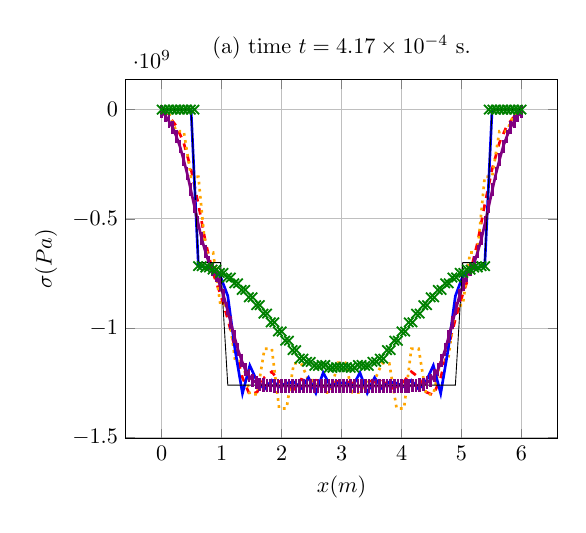
\begin{tikzpicture}[scale=0.8]
\begin{axis}[xlabel=$x (m)$,ylabel=$\sigma (Pa)$,ymajorgrids=true,xmajorgrids=true,legend pos=outer north east,title={(a) time $t = 4.17\times 10^{-4} $ s.}]
\addplot[Red,very thick,mark=none,dashed,mark size=3pt] coordinates {(0.0,-8613486.937425343) (0.12244897959183673,-32098082.523617607) (0.24489795918367346,-75184156.81448549) (0.36734693877551017,-152006982.04059458) (0.4897959183673469,-272918299.7571908) (0.6122448979591837,-434866115.3917057) (0.7346938775510203,-610982765.9130303) (0.8571428571428571,-748144953.2233859) (0.9795918367346939,-845561032.3267925) (1.1020408163265305,-958425749.0711806) (1.2244897959183674,-1093872940.3932045) (1.346938775510204,-1225940785.1464355) (1.4693877551020407,-1306595231.2314239) (1.5918367346938775,-1292395303.4332397) (1.7142857142857142,-1224981707.482427) (1.836734693877551,-1199290066.9091918) (1.9591836734693877,-1243789659.077468) (2.0816326530612246,-1268868931.2157116) (2.204081632653061,-1279555678.011958) (2.326530612244898,-1233843965.2013993) (2.4489795918367347,-1247141973.55301) (2.571428571428571,-1238578154.7331731) (2.693877551020408,-1267018472.19709) (2.816326530612245,-1251288495.1191645) (2.9387755102040813,-1243897445.9598322) (3.061224489795918,-1243897435.653917) (3.183673469387755,-1251288503.290518) (3.306122448979592,-1267018428.6038225) (3.4285714285714284,-1238578260.808024) (3.5510204081632653,-1247141795.020678) (3.673469387755102,-1233843980.264652) (3.7959183673469385,-1279555708.0603902) (3.9183673469387754,-1268868951.8947906) (4.040816326530612,-1243789871.0589092) (4.163265306122449,-1199290088.7219405) (4.285714285714286,-1224981642.7661428) (4.408163265306122,-1292395301.959645) (4.530612244897959,-1306595226.543051) (4.653061224489796,-1225940771.116342) (4.775510204081632,-1093872923.6488597) (4.8979591836734695,-958425734.4341587) (5.020408163265306,-845561024.6840333) (5.142857142857142,-748144947.3854173) (5.26530612244898,-610982760.9679779) (5.387755102040816,-434866113.85137385) (5.5102040816326525,-272918299.19915956) (5.63265306122449,-152006981.87613484) (5.755102040816326,-75184156.77668796) (5.877551020408163,-32098082.517845426) (6.0,-8613486.937112756) };
\addplot[Orange,very thick,mark=none,dotted,mark size=3pt] coordinates {(0.0,-19486450.00530802) (0.12244897959183673,-19486451.37255413) (0.24489795918367346,-98883525.16193365) (0.36734693877551017,-98883532.35877307) (0.4897959183673469,-307042948.5329649) (0.6122448979591837,-307042973.8393218) (0.7346938775510203,-653662753.2107606) (0.8571428571428571,-653662791.3443154) (0.9795918367346939,-895033212.2083819) (1.1020408163265305,-895033210.2294395) (1.2244897959183674,-1149711785.0376468) (1.346938775510204,-1149711707.6439426) (1.4693877551020407,-1302739092.3749402) (1.5918367346938775,-1302739042.5575087) (1.7142857142857142,-1094479333.510092) (1.836734693877551,-1094479363.641839) (1.9591836734693877,-1367729442.0453632) (2.0816326530612246,-1367729367.5886066) (2.204081632653061,-1161379499.150298) (2.326530612244898,-1161379598.2026331) (2.4489795918367347,-1238878624.5589573) (2.571428571428571,-1238878689.4608257) (2.693877551020408,-1294478206.9174366) (2.816326530612245,-1294478350.007934) (2.9387755102040813,-1158113298.5889149) (3.061224489795918,-1158113331.6700864) (3.183673469387755,-1294477877.3735123) (3.306122448979592,-1294477954.2759767) (3.4285714285714284,-1238878389.3714159) (3.5510204081632653,-1238878336.5056608) (3.673469387755102,-1161379397.0010178) (3.7959183673469385,-1161379295.220285) (3.9183673469387754,-1367729506.3247807) (4.040816326530612,-1367729486.415212) (4.163265306122449,-1094479488.8470607) (4.285714285714286,-1094479504.218566) (4.408163265306122,-1302739089.2586887) (4.530612244897959,-1302739090.6284595) (4.653061224489796,-1149711763.4099293) (4.775510204081632,-1149711761.6734378) (4.8979591836734695,-895033202.7697786) (5.020408163265306,-895033202.8404319) (5.142857142857142,-653662748.8713347) (5.26530612244898,-653662750.5779299) (5.387755102040816,-307042947.2123353) (5.5102040816326525,-307042947.98137856) (5.63265306122449,-98883524.96726042) (5.755102040816326,-98883525.08736782) (5.877551020408163,-19486450.128640544) (6.0,-19486450.13761897) };
\addplot[Blue,very thick,mark=none,solid,mark size=3pt] coordinates {(0.0,-6.648826343127885e-07) (0.12244897959183673,4.986619757345916e-07) (0.24489795918367346,-6.648826343127894e-07) (0.36734693877551017,6.648826343127889e-07) (0.4897959183673469,-3.324413171563951e-07) (0.6122448979591837,-715667367.438887) (0.7346938775510203,-721624002.2150931) (0.8571428571428571,-733440346.5979226) (0.9795918367346939,-762779433.8121859) (1.1020408163265305,-852759583.0719095) (1.2244897959183674,-1101085033.4809394) (1.346938775510204,-1298836944.1354702) (1.4693877551020407,-1171100114.2056987) (1.5918367346938775,-1244615764.4304001) (1.7142857142857142,-1279401316.71709) (1.836734693877551,-1238612976.7167482) (1.9591836734693877,-1268822286.952483) (2.0816326530612246,-1251851454.2582784) (2.204081632653061,-1246344358.2784605) (2.326530612244898,-1274636654.590367) (2.4489795918367347,-1226444366.5447345) (2.571428571428571,-1297309357.6096141) (2.693877551020408,-1203729922.9079342) (2.816326530612245,-1267608663.445644) (2.9387755102040813,-1250429639.6986516) (3.061224489795918,-1250429639.698652) (3.183673469387755,-1267608663.4456437) (3.306122448979592,-1203729922.9079332) (3.4285714285714284,-1297309357.6096146) (3.5510204081632653,-1226444366.5447364) (3.673469387755102,-1274636654.5903707) (3.7959183673469385,-1246344358.2784586) (3.9183673469387754,-1251851454.2582788) (4.040816326530612,-1268822286.952483) (4.163265306122449,-1238612976.716749) (4.285714285714286,-1279401316.717093) (4.408163265306122,-1244615764.4303992) (4.530612244897959,-1171100114.205699) (4.653061224489796,-1298836944.1354706) (4.775510204081632,-1101085033.480938) (4.8979591836734695,-852759583.0719106) (5.020408163265306,-762779433.8121861) (5.142857142857142,-733440346.5979232) (5.26530612244898,-721624002.2150935) (5.387755102040816,-715667367.4388872) (5.5102040816326525,6.648826343127891e-07) (5.63265306122449,-8.311032928909869e-07) (5.755102040816326,6.64882634312789e-07) (5.877551020408163,-4.986619757345927e-07) (6.0,6.648826343127891e-07) };
\addplot[Purple,very thick,mark=|,solid,mark size=3pt] coordinates {(0.0,-10102308.696129723) (0.06060606060606061,-27819035.408597022) (0.12121212121212122,-53548174.10156911) (0.18181818181818182,-81220530.91552682) (0.24242424242424243,-121996638.1282555) (0.30303030303030304,-167271442.91399714) (0.36363636363636365,-227374416.8224694) (0.42424242424242425,-291884207.62740797) (0.48484848484848486,-366561331.82425076) (0.5454545454545454,-442651846.10117203) (0.6060606060606061,-517981788.6506681) (0.6666666666666667,-590163308.883224) (0.7272727272727273,-649294423.8320683) (0.7878787878787878,-701741095.1196218) (0.8484848484848485,-730769282.7949975) (0.9090909090909092,-756872056.3761383) (0.9696969696969697,-801569181.7407509) (1.0303030303030303,-849177673.0800432) (1.0909090909090908,-911084939.7727154) (1.1515151515151516,-974214002.7169627) (1.2121212121212122,-1038167680.0536075) (1.2727272727272727,-1099090105.6739883) (1.3333333333333335,-1147307672.5705764) (1.393939393939394,-1190753537.809418) (1.4545454545454546,-1216875899.9474456) (1.5151515151515151,-1239215801.8963046) (1.5757575757575757,-1249066695.0125978) (1.6363636363636365,-1257474117.1450398) (1.696969696969697,-1260287231.5732214) (1.7575757575757576,-1262882155.5942452) (1.8181818181818183,-1263639434.435723) (1.878787878787879,-1264451227.6039906) (1.9393939393939394,-1264700974.3286438) (2.0,-1264995274.0914948) (2.0606060606060606,-1265081753.3010664) (2.121212121212121,-1265196971.579899) (2.1818181818181817,-1265214637.004615) (2.2424242424242427,-1265254598.958957) (2.303030303030303,-1265245140.1058884) (2.3636363636363638,-1265256293.5490305) (2.4242424242424243,-1265242505.3887954) (2.484848484848485,-1265248286.884651) (2.5454545454545454,-1265240360.2874153) (2.606060606060606,-1265250508.029845) (2.666666666666667,-1265248914.1312644) (2.7272727272727275,-1265263548.0936751) (2.787878787878788,-1265262744.314047) (2.8484848484848486,-1265286671.3434186) (2.909090909090909,-1265283781.3906841) (2.9696969696969697,-1265290450.4639096) (3.0303030303030303,-1265290450.4639094) (3.090909090909091,-1265283781.3906841) (3.1515151515151514,-1265286671.3434184) (3.2121212121212124,-1265262744.3140473) (3.272727272727273,-1265263548.0936751) (3.3333333333333335,-1265248914.1312644) (3.393939393939394,-1265250508.029845) (3.4545454545454546,-1265240360.2874155) (3.515151515151515,-1265248286.884651) (3.5757575757575757,-1265242505.3887959) (3.6363636363636367,-1265256293.5490305) (3.6969696969696972,-1265245140.1058888) (3.757575757575758,-1265254598.9589574) (3.8181818181818183,-1265214637.0046158) (3.878787878787879,-1265196971.5798993) (3.9393939393939394,-1265081753.301067) (4.0,-1264995274.0914955) (4.0606060606060606,-1264700974.3286445) (4.121212121212121,-1264451227.603991) (4.181818181818182,-1263639434.4357235) (4.242424242424242,-1262882155.5942454) (4.303030303030303,-1260287231.5732222) (4.363636363636363,-1257474117.1450403) (4.424242424242425,-1249066695.0125985) (4.484848484848485,-1239215801.896305) (4.545454545454546,-1216875899.9474466) (4.606060606060606,-1190753537.8094187) (4.666666666666667,-1147307672.5705774) (4.7272727272727275,-1099090105.6739895) (4.787878787878788,-1038167680.053609) (4.848484848484849,-974214002.7169627) (4.909090909090909,-911084939.772716) (4.96969696969697,-849177673.0800438) (5.03030303030303,-801569181.7407513) (5.090909090909091,-756872056.3761387) (5.151515151515151,-730769282.7949976) (5.212121212121212,-701741095.1196221) (5.2727272727272725,-649294423.8320689) (5.333333333333334,-590163308.8832242) (5.3939393939393945,-517981788.6506686) (5.454545454545455,-442651846.10117245) (5.515151515151516,-366561331.82425123) (5.575757575757576,-291884207.62740815) (5.636363636363637,-227374416.82246974) (5.696969696969697,-167271442.91399717) (5.757575757575758,-121996638.12825578) (5.818181818181818,-81220530.91552722) (5.878787878787879,-53548174.101569325) (5.9393939393939394,-27819035.408597216) (6.0,-10102308.696129855) };
\addplot[Green,thick,mark=x,only marks,mark size=3pt] coordinates {(0.0,-2.0877147917780336e-07) (0.06060606060606061,-1.23669837978591e-07) (0.12121212121212122,1.0131895444177197e-06) (0.18181818181818182,9.814583585206487e-07) (0.24242424242424243,-5.619879278457838e-07) (0.30303030303030304,-7.677773407797948e-07) (0.36363636363636365,4.815476698956227e-07) (0.42424242424242425,1.8333496441716677e-07) (0.48484848484848486,1.0440135561077701e-07) (0.5454545454545454,2.2803996154561766e-07) (0.6060606060606061,-716376930.5893724) (0.6666666666666667,-716376930.589367) (0.7272727272727273,-722477457.3590242) (0.7878787878787878,-722477457.3590261) (0.8484848484848485,-732178472.6355962) (0.9090909090909092,-732178472.6355944) (0.9696969696969697,-747351730.2863077) (1.0303030303030303,-747351730.2863119) (1.0909090909090908,-768562816.0383832) (1.1515151515151516,-768562816.0383828) (1.2121212121212122,-794945415.8744416) (1.2727272727272727,-794945415.8744432) (1.3333333333333335,-825275759.4899069) (1.393939393939394,-825275759.4899055) (1.4545454545454546,-858914148.2093647) (1.5151515151515151,-858914148.2093657) (1.5757575757575757,-895001130.8125886) (1.6363636363636365,-895001130.8125875) (1.696969696969697,-933584126.6213479) (1.7575757575757576,-933584126.6213498) (1.8181818181818183,-973568810.43142) (1.878787878787879,-973568810.4314172) (1.9393939393939394,-1015496794.5721984) (2.0,-1015496794.57219) (2.0606060606060606,-1057685588.3287526) (2.121212121212121,-1057685588.3287554) (2.1818181818181817,-1100692545.9682453) (2.2424242424242427,-1100692545.968236) (2.303030303030303,-1139792908.6344922) (2.3636363636363638,-1139792908.6344938) (2.4242424242424243,-1154354135.2303133) (2.484848484848485,-1154354135.2299874) (2.5454545454545454,-1172832255.3077557) (2.606060606060606,-1172832255.3077602) (2.666666666666667,-1168855409.3584068) (2.7272727272727275,-1168855409.358407) (2.787878787878788,-1181372468.846199) (2.8484848484848486,-1181372468.8461988) (2.909090909090909,-1178905236.4784043) (2.9696969696969697,-1178905236.4784184) (3.0303030303030303,-1178905236.4783716) (3.090909090909091,-1178905236.4783936) (3.1515151515151514,-1181372468.8462052) (3.2121212121212124,-1181372468.8462112) (3.272727272727273,-1168855409.3585627) (3.3333333333333335,-1168855409.3585649) (3.393939393939394,-1172832255.307782) (3.4545454545454546,-1172832255.3077602) (3.515151515151515,-1154354135.2301552) (3.5757575757575757,-1154354135.2301497) (3.6363636363636367,-1139792908.6344705) (3.6969696969696972,-1139792908.6344807) (3.757575757575758,-1100692545.9682417) (3.8181818181818183,-1100692545.968244) (3.878787878787879,-1057685588.3287588) (3.9393939393939394,-1057685588.3287547) (4.0,-1015496794.572189) (4.0606060606060606,-1015496794.5721911) (4.121212121212121,-973568810.4314169) (4.181818181818182,-973568810.4314196) (4.242424242424242,-933584126.6213472) (4.303030303030303,-933584126.6213481) (4.363636363636363,-895001130.8125902) (4.424242424242425,-895001130.8125896) (4.484848484848485,-858914148.2093651) (4.545454545454546,-858914148.2093666) (4.606060606060606,-825275759.4899112) (4.666666666666667,-825275759.4899105) (4.7272727272727275,-794945415.8744518) (4.787878787878788,-794945415.8744564) (4.848484848484849,-768562816.0383911) (4.909090909090909,-768562816.0383939) (4.96969696969697,-747351730.286324) (5.03030303030303,-747351730.2863271) (5.090909090909091,-732178472.6356105) (5.151515151515151,-732178472.6356128) (5.212121212121212,-722477457.3590274) (5.2727272727272725,-722477457.3590299) (5.333333333333334,-716376930.5893677) (5.3939393939393945,-716376930.5893692) (5.454545454545455,6.698192810303248e-07) (5.515151515151516,6.599459875952535e-07) (5.575757575757576,-9.369788715662316e-07) (5.636363636363637,-1.0576690313721361e-06) (5.696969696969697,1.675441116120912e-06) (5.757575757575758,1.6489720554430353e-06) (5.818181818181818,-1.0608989471845062e-06) (5.878787878787879,-9.337489557538617e-07) (5.9393939393939394,1.4751713795395358e-06) (6.0,1.5168004748680168e-06) };
\addplot[black,thin,mark=none,solid,mark size=3pt] coordinates {(0.0,-0.0) (0.12244897959183673,-0.0) (0.24489795918367346,-0.0) (0.36734693877551017,-0.0) (0.4897959183673469,-0.0) (0.6122448979591837,-700000000.0) (0.7346938775510203,-700000000.0) (0.8571428571428571,-700000000.0) (0.9795918367346939,-700000000.0) (1.1020408163265305,-1261004576.260559) (1.2244897959183674,-1261004576.260559) (1.346938775510204,-1261004576.260559) (1.4693877551020407,-1261004576.260559) (1.5918367346938775,-1261004576.260559) (1.7142857142857142,-1261004576.260559) (1.836734693877551,-1261004576.260559) (1.9591836734693877,-1261004576.260559) (2.0816326530612246,-1261004576.260559) (2.204081632653061,-1261004576.260559) (2.326530612244898,-1261004576.260559) (2.4489795918367347,-1261004576.260559) (2.571428571428571,-1261004576.260559) (2.693877551020408,-1261004576.260559) (2.816326530612245,-1261004576.260559) (2.9387755102040813,-1261004576.260559) (3.061224489795918,-1261004576.260559) (3.183673469387755,-1261004576.260559) (3.306122448979592,-1261004576.260559) (3.4285714285714284,-1261004576.260559) (3.5510204081632653,-1261004576.260559) (3.673469387755102,-1261004576.260559) (3.7959183673469385,-1261004576.260559) (3.9183673469387754,-1261004576.260559) (4.040816326530612,-1261004576.260559) (4.163265306122449,-1261004576.260559) (4.285714285714286,-1261004576.260559) (4.408163265306122,-1261004576.260559) (4.530612244897959,-1261004576.260559) (4.653061224489796,-1261004576.260559) (4.775510204081632,-1261004576.260559) (4.8979591836734695,-1261004576.260559) (5.020408163265306,-700000000.0) (5.142857142857142,-700000000.0) (5.26530612244898,-700000000.0) (5.387755102040816,-700000000.0) (5.5102040816326525,-0.0) (5.63265306122449,-0.0) (5.755102040816326,-0.0) (5.877551020408163,-0.0) (6.0,-0.0) };
%\legend{usl 1ppc,usf 1ppc,dgmpm 1ppc,dgmpm 2ppc,dgmpm 2ppc (RK2 + strang),plastic solution}
\end{axis}
\end{tikzpicture}
%%% Local Variables:
%%% mode: latex
%%% TeX-master: "../../mainManuscript"
%%% End:
}
  % {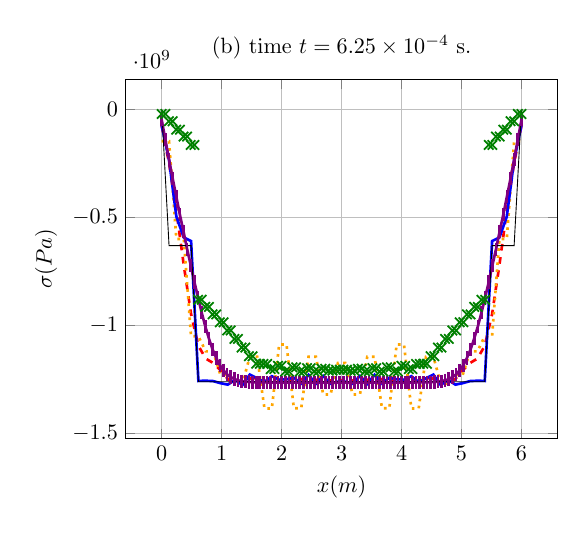
\begin{tikzpicture}[scale=0.8]
\begin{axis}[xlabel=$x (m)$,ylabel=$\sigma (Pa)$,ymajorgrids=true,xmajorgrids=true,legend pos=outer north east,title={(b) time $t = 6.25\times 10^{-4} $ s.}]
\addplot[Red,very thick,mark=none,dashed,mark size=3pt] coordinates {(0.0,-74755364.74533166) (0.12244897959183673,-248208896.12486583) (0.24489795918367346,-468625717.803481) (0.36734693877551017,-719013533.7365903) (0.4897959183673469,-947742026.6398356) (0.6122448979591837,-1094792437.4560761) (0.7346938775510203,-1153839566.2578583) (0.8571428571428571,-1174113393.2907) (0.9795918367346939,-1207454154.8556237) (1.1020408163265305,-1248053189.0341141) (1.2244897959183674,-1269531290.7275531) (1.346938775510204,-1257538829.8363345) (1.4693877551020407,-1246174055.5311027) (1.5918367346938775,-1243899733.863632) (1.7142857142857142,-1257815798.8450537) (1.836734693877551,-1259247134.6249063) (1.9591836734693877,-1263208926.5266936) (2.0816326530612246,-1248288130.419574) (2.204081632653061,-1261500638.8122087) (2.326530612244898,-1248516389.0385368) (2.4489795918367347,-1265795229.6578722) (2.571428571428571,-1251562844.0674527) (2.693877551020408,-1262749976.8464308) (2.816326530612245,-1255375541.0724187) (2.9387755102040813,-1253751855.6811213) (3.061224489795918,-1253751839.0824046) (3.183673469387755,-1255375534.8022113) (3.306122448979592,-1262749921.7411852) (3.4285714285714284,-1251562950.169376) (3.5510204081632653,-1265795057.7459216) (3.673469387755102,-1248516391.9733808) (3.7959183673469385,-1261500630.050308) (3.9183673469387754,-1248288097.1119542) (4.040816326530612,-1263209080.4260836) (4.163265306122449,-1259247117.6459212) (4.285714285714286,-1257815707.7658777) (4.408163265306122,-1243899712.3822339) (4.530612244897959,-1246174035.7380946) (4.653061224489796,-1257539140.237503) (4.775510204081632,-1269531234.7005646) (4.8979591836734695,-1248053690.7012877) (5.020408163265306,-1207453700.9419231) (5.142857142857142,-1174113502.2223024) (5.26530612244898,-1153838796.8971734) (5.387755102040816,-1094792530.955986) (5.5102040816326525,-947741675.2773904) (5.63265306122449,-719013481.172835) (5.755102040816326,-468625706.5592639) (5.877551020408163,-248208829.82757288) (6.0,-74755344.97904286) };
\addplot[Orange,very thick,mark=none,dotted,mark size=3pt] coordinates {(0.0,-146910686.54340002) (0.12244897959183673,-146910576.6778985) (0.24489795918367346,-599499161.4545292) (0.36734693877551017,-599499345.0291598) (0.4897959183673469,-1050556946.940909) (0.6122448979591837,-1050556810.8531282) (0.7346938775510203,-1120414463.9040096) (0.8571428571428571,-1120414507.6770024) (0.9795918367346939,-1229455185.2009192) (1.1020408163265305,-1229455106.2082894) (1.2244897959183674,-1269042253.7721956) (1.346938775510204,-1269042214.6789474) (1.4693877551020407,-1144813454.0089188) (1.5918367346938775,-1144813966.490456) (1.7142857142857142,-1385034660.973245) (1.836734693877551,-1385034240.6909063) (1.9591836734693877,-1088744428.4000087) (2.0816326530612246,-1088744356.7882442) (2.204081632653061,-1383996748.4707298) (2.326530612244898,-1383996722.000206) (2.4489795918367347,-1144999088.7730293) (2.571428571428571,-1144998814.9657073) (2.693877551020408,-1320236218.1167607) (2.816326530612245,-1320236958.4771528) (2.9387755102040813,-1174522093.1728597) (3.061224489795918,-1174521439.5484982) (3.183673469387755,-1320235859.9132228) (3.306122448979592,-1320235657.2910552) (3.4285714285714284,-1145000190.5115752) (3.5510204081632653,-1144999698.2190187) (3.673469387755102,-1383996750.799452) (3.7959183673469385,-1383996409.8226683) (3.9183673469387754,-1088744644.3503904) (4.040816326530612,-1088744177.3418117) (4.163265306122449,-1385034239.357628) (4.285714285714286,-1385034463.0774357) (4.408163265306122,-1144813430.515698) (4.530612244897959,-1144813914.0897422) (4.653061224489796,-1269041947.1103678) (4.775510204081632,-1269041892.7174592) (4.8979591836734695,-1229455306.2104805) (5.020408163265306,-1229455419.0438316) (5.142857142857142,-1120414629.727034) (5.26530612244898,-1120414606.2420225) (5.387755102040816,-1050556872.9115263) (5.5102040816326525,-1050556814.2558659) (5.63265306122449,-599499269.4389613) (5.755102040816326,-599499363.047376) (5.877551020408163,-146910684.6411048) (6.0,-146910614.3275735) };
\addplot[Blue,very thick,mark=none,solid,mark size=3pt] coordinates {(0.0,-73372434.82033628) (0.12244897959183673,-233858719.55212942) (0.24489795918367346,-495938295.48681855) (0.36734693877551017,-592504781.1553047) (0.4897959183673469,-609199055.9406189) (0.6122448979591837,-1257272451.0662038) (0.7346938775510203,-1256464300.2954264) (0.8571428571428571,-1258068523.1986136) (0.9795918367346939,-1267655174.0427077) (1.1020408163265305,-1274486401.3694665) (1.2244897959183674,-1252604107.07487) (1.346938775510204,-1276531816.9026763) (1.4693877551020407,-1227937227.7003279) (1.5918367346938775,-1245313491.0436618) (1.7142857142857142,-1262325040.1928196) (1.836734693877551,-1235608282.656636) (1.9591836734693877,-1251386670.8684802) (2.0816326530612246,-1249617525.1753566) (2.204081632653061,-1242442736.3652022) (2.326530612244898,-1269356567.5147986) (2.4489795918367347,-1229053885.1472373) (2.571428571428571,-1271114130.25009) (2.693877551020408,-1234588132.0907624) (2.816326530612245,-1270149960.4084883) (2.9387755102040813,-1260862894.9637291) (3.061224489795918,-1260862894.963727) (3.183673469387755,-1270149960.4084873) (3.306122448979592,-1234588132.0907636) (3.4285714285714284,-1271114130.2500923) (3.5510204081632653,-1229053885.1472325) (3.673469387755102,-1269356567.5148) (3.7959183673469385,-1242442736.3652017) (3.9183673469387754,-1249617525.1753573) (4.040816326530612,-1251386670.8684816) (4.163265306122449,-1235608282.6566362) (4.285714285714286,-1262325040.1928182) (4.408163265306122,-1245313491.0436635) (4.530612244897959,-1227937227.7003253) (4.653061224489796,-1276531816.9026778) (4.775510204081632,-1252604107.074872) (4.8979591836734695,-1274486401.3694673) (5.020408163265306,-1267655174.0427058) (5.142857142857142,-1258068523.1986136) (5.26530612244898,-1256464300.2954257) (5.387755102040816,-1257272451.0662048) (5.5102040816326525,-609199055.940622) (5.63265306122449,-592504781.1553006) (5.755102040816326,-495938295.48681825) (5.877551020408163,-233858719.55212817) (6.0,-73372434.82033731) };
\addplot[Purple,very thick,mark=|,solid,mark size=3pt] coordinates {(0.0,-47333356.22779358) (0.06060606060606061,-138756545.0597926) (0.12121212121212122,-229985791.05287215) (0.18181818181818182,-318140237.4578) (0.24242424242424243,-402202061.10697633) (0.30303030303030304,-486791312.40641415) (0.36363636363636365,-564994266.2878431) (0.42424242424242425,-646698716.5243026) (0.48484848484848486,-721593111.9376383) (0.5454545454545454,-799220239.6164875) (0.6060606060606061,-870833555.6318947) (0.6666666666666667,-940547799.3769101) (0.7272727272727273,-1004764341.06167) (0.7878787878787878,-1060903097.5027591) (0.8484848484848485,-1111526011.847744) (0.9090909090909092,-1150516460.50863) (0.9696969696969697,-1184534064.1013935) (1.0303030303030303,-1207708133.016495) (1.0909090909090908,-1227220308.6256344) (1.1515151515151516,-1239136300.842325) (1.2121212121212122,-1248834908.9252155) (1.2727272727272727,-1254207515.376704) (1.3333333333333335,-1258429252.1271956) (1.393939393939394,-1260585212.884834) (1.4545454545454546,-1262234236.0930166) (1.5151515151515151,-1263047159.404436) (1.5757575757575757,-1263653386.8297281) (1.6363636363636365,-1263951357.5622544) (1.696969696969697,-1264163825.8617294) (1.7575757575757576,-1264271933.08496) (1.8181818181818183,-1264341903.226051) (1.878787878787879,-1264380965.5508432) (1.9393939393939394,-1264400307.6802652) (2.0,-1264413367.7497914) (2.0606060606060606,-1264414399.1473076) (2.121212121212121,-1264416892.3074598) (2.1818181818181817,-1264411289.2771008) (2.2424242424242427,-1264409453.8903484) (2.303030303030303,-1264402104.3991406) (2.3636363636363638,-1264399159.0796075) (2.4242424242424243,-1264392461.8213086) (2.484848484848485,-1264390501.27199) (2.5454545454545454,-1264385501.2848275) (2.606060606060606,-1264385712.5692852) (2.666666666666667,-1264382271.7032228) (2.7272727272727275,-1264384650.233929) (2.787878787878788,-1264381389.2284317) (2.8484848484848486,-1264388956.0046396) (2.909090909090909,-1264385898.768779) (2.9696969696969697,-1264387667.9110923) (3.0303030303030303,-1264387667.911092) (3.090909090909091,-1264385898.768779) (3.1515151515151514,-1264388956.0046391) (3.2121212121212124,-1264381389.2284312) (3.272727272727273,-1264384650.2339287) (3.3333333333333335,-1264382271.7032225) (3.393939393939394,-1264385712.569285) (3.4545454545454546,-1264385501.2848277) (3.515151515151515,-1264390501.2719903) (3.5757575757575757,-1264392461.8213089) (3.6363636363636367,-1264399159.0796077) (3.6969696969696972,-1264402104.399141) (3.757575757575758,-1264409453.8903487) (3.8181818181818183,-1264411289.277101) (3.878787878787879,-1264416892.30746) (3.9393939393939394,-1264414399.1473076) (4.0,-1264413367.7497916) (4.0606060606060606,-1264400307.6802652) (4.121212121212121,-1264380965.5508432) (4.181818181818182,-1264341903.2260516) (4.242424242424242,-1264271933.0849605) (4.303030303030303,-1264163825.8617299) (4.363636363636363,-1263951357.5622554) (4.424242424242425,-1263653386.8297288) (4.484848484848485,-1263047159.4044366) (4.545454545454546,-1262234236.093017) (4.606060606060606,-1260585212.8848348) (4.666666666666667,-1258429252.127196) (4.7272727272727275,-1254207515.3767045) (4.787878787878788,-1248834908.925216) (4.848484848484849,-1239136300.8423254) (4.909090909090909,-1227220308.6256351) (4.96969696969697,-1207708133.0164952) (5.03030303030303,-1184534064.1013935) (5.090909090909091,-1150516460.50863) (5.151515151515151,-1111526011.847744) (5.212121212121212,-1060903097.5027591) (5.2727272727272725,-1004764341.0616697) (5.333333333333334,-940547799.3769101) (5.3939393939393945,-870833555.6318948) (5.454545454545455,-799220239.6164877) (5.515151515151516,-721593111.9376383) (5.575757575757576,-646698716.5243028) (5.636363636363637,-564994266.2878435) (5.696969696969697,-486791312.4064143) (5.757575757575758,-402202061.1069768) (5.818181818181818,-318140237.4578002) (5.878787878787879,-229985791.0528724) (5.9393939393939394,-138756545.05979264) (6.0,-47333356.22779366) };
\addplot[Green,thick,mark=x,only marks,mark size=3pt] coordinates {(0.0,-20229275.520624813) (0.06060606060606061,-20229275.520624828) (0.12121212121212122,-53902709.192570105) (0.18181818181818182,-53902709.192569956) (0.24242424242424243,-93046882.15578794) (0.30303030303030304,-93046882.1557879) (0.36363636363636365,-124818495.63572057) (0.42424242424242425,-124818495.6357201) (0.48484848484848486,-163811216.3609897) (0.5454545454545454,-163811216.36098817) (0.6060606060606061,-881303240.5770407) (0.6666666666666667,-881303240.5770347) (0.7272727272727273,-914303290.6106135) (0.7878787878787878,-914303290.610614) (0.8484848484848485,-949108866.3150425) (0.9090909090909092,-949108866.3150418) (0.9696969696969697,-985587474.2698758) (1.0303030303030303,-985587474.2698789) (1.0909090909090908,-1023460684.7529197) (1.1515151515151516,-1023460684.7529227) (1.2121212121212122,-1062676463.9811376) (1.2727272727272727,-1062676463.9811432) (1.3333333333333335,-1102710418.5537071) (1.393939393939394,-1102710418.553707) (1.4545454545454546,-1142958071.2150478) (1.5151515151515151,-1142958071.2150497) (1.5757575757575757,-1177713108.448572) (1.6363636363636365,-1177713108.4485712) (1.696969696969697,-1178607832.5129364) (1.7575757575757576,-1178607832.5129366) (1.8181818181818183,-1202493123.9660535) (1.878787878787879,-1202493123.966045) (1.9393939393939394,-1187462459.6258917) (2.0,-1187462459.6258917) (2.0606060606060606,-1213334125.432626) (2.121212121212121,-1213334125.4325962) (2.1818181818181817,-1194303471.3523695) (2.2424242424242427,-1194303471.35237) (2.303030303030303,-1213800467.2016068) (2.3636363636363638,-1213800467.201615) (2.4242424242424243,-1198169738.036603) (2.484848484848485,-1198169738.036608) (2.5454545454545454,-1213000678.5547864) (2.606060606060606,-1213000678.5547855) (2.666666666666667,-1201083468.1228912) (2.7272727272727275,-1201083468.122941) (2.787878787878788,-1210046074.450863) (2.8484848484848486,-1210046074.4508822) (2.909090909090909,-1205397510.3980381) (2.9696969696969697,-1205397510.3980904) (3.0303030303030303,-1205397510.3980312) (3.090909090909091,-1205397510.3980837) (3.1515151515151514,-1210046074.4509275) (3.2121212121212124,-1210046074.450946) (3.272727272727273,-1201083468.122753) (3.3333333333333335,-1201083468.1228034) (3.393939393939394,-1213000678.5547462) (3.4545454545454546,-1213000678.5547454) (3.515151515151515,-1198169738.0364976) (3.5757575757575757,-1198169738.0364983) (3.6363636363636367,-1213800467.20157) (3.6969696969696972,-1213800467.2015686) (3.757575757575758,-1194303471.3523912) (3.8181818181818183,-1194303471.3523917) (3.878787878787879,-1213334125.432576) (3.9393939393939394,-1213334125.432606) (4.0,-1187462459.6258657) (4.0606060606060606,-1187462459.625866) (4.121212121212121,-1202493123.966091) (4.181818181818182,-1202493123.966098) (4.242424242424242,-1178607832.513093) (4.303030303030303,-1178607832.5130925) (4.363636363636363,-1177713108.448581) (4.424242424242425,-1177713108.4485826) (4.484848484848485,-1142958071.215055) (4.545454545454546,-1142958071.2150486) (4.606060606060606,-1102710418.5537033) (4.666666666666667,-1102710418.5537047) (4.7272727272727275,-1062676463.9811467) (4.787878787878788,-1062676463.9811449) (4.848484848484849,-1023460684.7529202) (4.909090909090909,-1023460684.7529212) (4.96969696969697,-985587474.2698778) (5.03030303030303,-985587474.2698749) (5.090909090909091,-949108866.315046) (5.151515151515151,-949108866.3150446) (5.212121212121212,-914303290.6106138) (5.2727272727272725,-914303290.6106144) (5.333333333333334,-881303240.5770384) (5.3939393939393945,-881303240.5770377) (5.454545454545455,-163811216.3609834) (5.515151515151516,-163811216.3609822) (5.575757575757576,-124818495.63570935) (5.636363636363637,-124818495.63570964) (5.696969696969697,-93046882.15578243) (5.757575757575758,-93046882.15578227) (5.818181818181818,-53902709.192592174) (5.878787878787879,-53902709.19259214) (5.9393939393939394,-20229275.520634342) (6.0,-20229275.520634633) };
\addplot[black,thin,mark=none,solid,mark size=3pt] coordinates {(0.0,-0.0) (0.12244897959183673,-630502288.1302795) (0.24489795918367346,-630502288.1302795) (0.36734693877551017,-630502288.1302795) (0.4897959183673469,-630502288.1302795) (0.6122448979591837,-1261004576.260559) (0.7346938775510203,-1261004576.260559) (0.8571428571428571,-1261004576.260559) (0.9795918367346939,-1261004576.260559) (1.1020408163265305,-1261004576.260559) (1.2244897959183674,-1261004576.260559) (1.346938775510204,-1261004576.260559) (1.4693877551020407,-1261004576.260559) (1.5918367346938775,-1261004576.260559) (1.7142857142857142,-1261004576.260559) (1.836734693877551,-1261004576.260559) (1.9591836734693877,-1261004576.260559) (2.0816326530612246,-1261004576.260559) (2.204081632653061,-1261004576.260559) (2.326530612244898,-1261004576.260559) (2.4489795918367347,-1261004576.260559) (2.571428571428571,-1261004576.260559) (2.693877551020408,-1261004576.260559) (2.816326530612245,-1261004576.260559) (2.9387755102040813,-1261004576.260559) (3.061224489795918,-1261004576.260559) (3.183673469387755,-1261004576.260559) (3.306122448979592,-1261004576.260559) (3.4285714285714284,-1261004576.260559) (3.5510204081632653,-1261004576.260559) (3.673469387755102,-1261004576.260559) (3.7959183673469385,-1261004576.260559) (3.9183673469387754,-1261004576.260559) (4.040816326530612,-1261004576.260559) (4.163265306122449,-1261004576.260559) (4.285714285714286,-1261004576.260559) (4.408163265306122,-1261004576.260559) (4.530612244897959,-1261004576.260559) (4.653061224489796,-1261004576.260559) (4.775510204081632,-1261004576.260559) (4.8979591836734695,-1261004576.260559) (5.020408163265306,-1261004576.260559) (5.142857142857142,-1261004576.260559) (5.26530612244898,-1261004576.260559) (5.387755102040816,-1261004576.260559) (5.5102040816326525,-630502288.1302795) (5.63265306122449,-630502288.1302795) (5.755102040816326,-630502288.1302795) (5.877551020408163,-630502288.1302795) (6.0,-0.0) };
%\legend{usl 1ppc,usf 1ppc,dgmpm 1ppc,dgmpm 2ppc,dgmpm 2ppc (RK2 + strang),plastic solution}
\end{axis}
\end{tikzpicture}
%%% Local Variables:
%%% mode: latex
%%% TeX-master: "../../mainManuscript"
%%% End:
}
  {\begin{tikzpicture}[scale=.9]
\begin{groupplot}[group style={group size=3 by 2,
ylabels at=edge left, yticklabels at=edge left,horizontal sep=2.ex,
vertical sep=4ex,xticklabels at=edge bottom,xlabels at=edge bottom},
ymajorgrids=true,xmajorgrids=true,enlargelimits=0,xmin=0.,xmax=6.,xlabel=$x (m)$,
axis on top,scale only axis,width=0.32\linewidth
]
\nextgroupplot[title={(a) $t = 4.17\times 10^{-4} $ s.},ylabel=$\sigma (Pa)$,]
\addplot[Red,dashed,mark=none,very thick,mark size=2pt] coordinates{(0.0,-8613486.93743) (0.122448979592,-32098082.5236) (0.244897959184,-75184156.8145) (0.367346938776,-152006982.041) (0.489795918367,-272918299.757) (0.612244897959,-434866115.392) (0.734693877551,-610982765.913) (0.857142857143,-748144953.223) (0.979591836735,-845561032.327) (1.10204081633,-958425749.071) (1.22448979592,-1093872940.39) (1.34693877551,-1225940785.15) (1.4693877551,-1306595231.23) (1.59183673469,-1292395303.43) (1.71428571429,-1224981707.48) (1.83673469388,-1199290066.91) (1.95918367347,-1243789659.08) (2.08163265306,-1268868931.22) (2.20408163265,-1279555678.01) (2.32653061224,-1233843965.2) (2.44897959184,-1247141973.55) (2.57142857143,-1238578154.73) (2.69387755102,-1267018472.2) (2.81632653061,-1251288495.12) (2.9387755102,-1243897445.96) (3.0612244898,-1243897435.65) (3.18367346939,-1251288503.29) (3.30612244898,-1267018428.6) (3.42857142857,-1238578260.81) (3.55102040816,-1247141795.02) (3.67346938776,-1233843980.26) (3.79591836735,-1279555708.06) (3.91836734694,-1268868951.89) (4.04081632653,-1243789871.06) (4.16326530612,-1199290088.72) (4.28571428571,-1224981642.77) (4.40816326531,-1292395301.96) (4.5306122449,-1306595226.54) (4.65306122449,-1225940771.12) (4.77551020408,-1093872923.65) (4.89795918367,-958425734.434) (5.02040816327,-845561024.684) (5.14285714286,-748144947.385) (5.26530612245,-610982760.968) (5.38775510204,-434866113.851) (5.51020408163,-272918299.199) (5.63265306122,-152006981.876) (5.75510204082,-75184156.7767) (5.87755102041,-32098082.5178) (6.0,-8613486.93711) };
\addplot[Orange,dotted,mark=none,very thick,mark size=2pt] coordinates{(0.0,-19486450.0053) (0.122448979592,-19486451.3726) (0.244897959184,-98883525.1619) (0.367346938776,-98883532.3588) (0.489795918367,-307042948.533) (0.612244897959,-307042973.839) (0.734693877551,-653662753.211) (0.857142857143,-653662791.344) (0.979591836735,-895033212.208) (1.10204081633,-895033210.229) (1.22448979592,-1149711785.04) (1.34693877551,-1149711707.64) (1.4693877551,-1302739092.37) (1.59183673469,-1302739042.56) (1.71428571429,-1094479333.51) (1.83673469388,-1094479363.64) (1.95918367347,-1367729442.05) (2.08163265306,-1367729367.59) (2.20408163265,-1161379499.15) (2.32653061224,-1161379598.2) (2.44897959184,-1238878624.56) (2.57142857143,-1238878689.46) (2.69387755102,-1294478206.92) (2.81632653061,-1294478350.01) (2.9387755102,-1158113298.59) (3.0612244898,-1158113331.67) (3.18367346939,-1294477877.37) (3.30612244898,-1294477954.28) (3.42857142857,-1238878389.37) (3.55102040816,-1238878336.51) (3.67346938776,-1161379397.0) (3.79591836735,-1161379295.22) (3.91836734694,-1367729506.32) (4.04081632653,-1367729486.42) (4.16326530612,-1094479488.85) (4.28571428571,-1094479504.22) (4.40816326531,-1302739089.26) (4.5306122449,-1302739090.63) (4.65306122449,-1149711763.41) (4.77551020408,-1149711761.67) (4.89795918367,-895033202.77) (5.02040816327,-895033202.84) (5.14285714286,-653662748.871) (5.26530612245,-653662750.578) (5.38775510204,-307042947.212) (5.51020408163,-307042947.981) (5.63265306122,-98883524.9673) (5.75510204082,-98883525.0874) (5.87755102041,-19486450.1286) (6.0,-19486450.1376) };
\addplot[Blue,solid,mark=none,very thick,mark size=2pt] coordinates{(0.0,-6.64882634313e-07) (0.122448979592,4.98661975735e-07) (0.244897959184,-6.64882634313e-07) (0.367346938776,6.64882634313e-07) (0.489795918367,-3.32441317156e-07) (0.612244897959,-715667367.439) (0.734693877551,-721624002.215) (0.857142857143,-733440346.598) (0.979591836735,-762779433.812) (1.10204081633,-852759583.072) (1.22448979592,-1101085033.48) (1.34693877551,-1298836944.14) (1.4693877551,-1171100114.21) (1.59183673469,-1244615764.43) (1.71428571429,-1279401316.72) (1.83673469388,-1238612976.72) (1.95918367347,-1268822286.95) (2.08163265306,-1251851454.26) (2.20408163265,-1246344358.28) (2.32653061224,-1274636654.59) (2.44897959184,-1226444366.54) (2.57142857143,-1297309357.61) (2.69387755102,-1203729922.91) (2.81632653061,-1267608663.45) (2.9387755102,-1250429639.7) (3.0612244898,-1250429639.7) (3.18367346939,-1267608663.45) (3.30612244898,-1203729922.91) (3.42857142857,-1297309357.61) (3.55102040816,-1226444366.54) (3.67346938776,-1274636654.59) (3.79591836735,-1246344358.28) (3.91836734694,-1251851454.26) (4.04081632653,-1268822286.95) (4.16326530612,-1238612976.72) (4.28571428571,-1279401316.72) (4.40816326531,-1244615764.43) (4.5306122449,-1171100114.21) (4.65306122449,-1298836944.14) (4.77551020408,-1101085033.48) (4.89795918367,-852759583.072) (5.02040816327,-762779433.812) (5.14285714286,-733440346.598) (5.26530612245,-721624002.215) (5.38775510204,-715667367.439) (5.51020408163,6.64882634313e-07) (5.63265306122,-8.31103292891e-07) (5.75510204082,6.64882634313e-07) (5.87755102041,-4.98661975735e-07) (6.0,6.64882634313e-07) };
\addplot[Purple,solid,mark=|,very thick,mark size=2pt] coordinates{(0.0,-10102308.6961) (0.0606060606061,-27819035.4086) (0.121212121212,-53548174.1016) (0.181818181818,-81220530.9155) (0.242424242424,-121996638.128) (0.30303030303,-167271442.914) (0.363636363636,-227374416.822) (0.424242424242,-291884207.627) (0.484848484848,-366561331.824) (0.545454545455,-442651846.101) (0.606060606061,-517981788.651) (0.666666666667,-590163308.883) (0.727272727273,-649294423.832) (0.787878787879,-701741095.12) (0.848484848485,-730769282.795) (0.909090909091,-756872056.376) (0.969696969697,-801569181.741) (1.0303030303,-849177673.08) (1.09090909091,-911084939.773) (1.15151515152,-974214002.717) (1.21212121212,-1038167680.05) (1.27272727273,-1099090105.67) (1.33333333333,-1147307672.57) (1.39393939394,-1190753537.81) (1.45454545455,-1216875899.95) (1.51515151515,-1239215801.9) (1.57575757576,-1249066695.01) (1.63636363636,-1257474117.15) (1.69696969697,-1260287231.57) (1.75757575758,-1262882155.59) (1.81818181818,-1263639434.44) (1.87878787879,-1264451227.6) (1.93939393939,-1264700974.33) (2.0,-1264995274.09) (2.06060606061,-1265081753.3) (2.12121212121,-1265196971.58) (2.18181818182,-1265214637.0) (2.24242424242,-1265254598.96) (2.30303030303,-1265245140.11) (2.36363636364,-1265256293.55) (2.42424242424,-1265242505.39) (2.48484848485,-1265248286.88) (2.54545454545,-1265240360.29) (2.60606060606,-1265250508.03) (2.66666666667,-1265248914.13) (2.72727272727,-1265263548.09) (2.78787878788,-1265262744.31) (2.84848484848,-1265286671.34) (2.90909090909,-1265283781.39) (2.9696969697,-1265290450.46) (3.0303030303,-1265290450.46) (3.09090909091,-1265283781.39) (3.15151515152,-1265286671.34) (3.21212121212,-1265262744.31) (3.27272727273,-1265263548.09) (3.33333333333,-1265248914.13) (3.39393939394,-1265250508.03) (3.45454545455,-1265240360.29) (3.51515151515,-1265248286.88) (3.57575757576,-1265242505.39) (3.63636363636,-1265256293.55) (3.69696969697,-1265245140.11) (3.75757575758,-1265254598.96) (3.81818181818,-1265214637.0) (3.87878787879,-1265196971.58) (3.93939393939,-1265081753.3) (4.0,-1264995274.09) (4.06060606061,-1264700974.33) (4.12121212121,-1264451227.6) (4.18181818182,-1263639434.44) (4.24242424242,-1262882155.59) (4.30303030303,-1260287231.57) (4.36363636364,-1257474117.15) (4.42424242424,-1249066695.01) (4.48484848485,-1239215801.9) (4.54545454545,-1216875899.95) (4.60606060606,-1190753537.81) (4.66666666667,-1147307672.57) (4.72727272727,-1099090105.67) (4.78787878788,-1038167680.05) (4.84848484848,-974214002.717) (4.90909090909,-911084939.773) (4.9696969697,-849177673.08) (5.0303030303,-801569181.741) (5.09090909091,-756872056.376) (5.15151515152,-730769282.795) (5.21212121212,-701741095.12) (5.27272727273,-649294423.832) (5.33333333333,-590163308.883) (5.39393939394,-517981788.651) (5.45454545455,-442651846.101) (5.51515151515,-366561331.824) (5.57575757576,-291884207.627) (5.63636363636,-227374416.822) (5.69696969697,-167271442.914) (5.75757575758,-121996638.128) (5.81818181818,-81220530.9155) (5.87878787879,-53548174.1016) (5.93939393939,-27819035.4086) (6.0,-10102308.6961) };
\addplot[Green,only marks,mark=x,thick,mark size=2pt] coordinates{(0.0,-2.08771479178e-07) (0.0606060606061,-1.23669837979e-07) (0.121212121212,1.01318954442e-06) (0.181818181818,9.81458358521e-07) (0.242424242424,-5.61987927846e-07) (0.30303030303,-7.6777734078e-07) (0.363636363636,4.81547669896e-07) (0.424242424242,1.83334964417e-07) (0.484848484848,1.04401355611e-07) (0.545454545455,2.28039961546e-07) (0.606060606061,-716376930.589) (0.666666666667,-716376930.589) (0.727272727273,-722477457.359) (0.787878787879,-722477457.359) (0.848484848485,-732178472.636) (0.909090909091,-732178472.636) (0.969696969697,-747351730.286) (1.0303030303,-747351730.286) (1.09090909091,-768562816.038) (1.15151515152,-768562816.038) (1.21212121212,-794945415.874) (1.27272727273,-794945415.874) (1.33333333333,-825275759.49) (1.39393939394,-825275759.49) (1.45454545455,-858914148.209) (1.51515151515,-858914148.209) (1.57575757576,-895001130.813) (1.63636363636,-895001130.813) (1.69696969697,-933584126.621) (1.75757575758,-933584126.621) (1.81818181818,-973568810.431) (1.87878787879,-973568810.431) (1.93939393939,-1015496794.57) (2.0,-1015496794.57) (2.06060606061,-1057685588.33) (2.12121212121,-1057685588.33) (2.18181818182,-1100692545.97) (2.24242424242,-1100692545.97) (2.30303030303,-1139792908.63) (2.36363636364,-1139792908.63) (2.42424242424,-1154354135.23) (2.48484848485,-1154354135.23) (2.54545454545,-1172832255.31) (2.60606060606,-1172832255.31) (2.66666666667,-1168855409.36) (2.72727272727,-1168855409.36) (2.78787878788,-1181372468.85) (2.84848484848,-1181372468.85) (2.90909090909,-1178905236.48) (2.9696969697,-1178905236.48) (3.0303030303,-1178905236.48) (3.09090909091,-1178905236.48) (3.15151515152,-1181372468.85) (3.21212121212,-1181372468.85) (3.27272727273,-1168855409.36) (3.33333333333,-1168855409.36) (3.39393939394,-1172832255.31) (3.45454545455,-1172832255.31) (3.51515151515,-1154354135.23) (3.57575757576,-1154354135.23) (3.63636363636,-1139792908.63) (3.69696969697,-1139792908.63) (3.75757575758,-1100692545.97) (3.81818181818,-1100692545.97) (3.87878787879,-1057685588.33) (3.93939393939,-1057685588.33) (4.0,-1015496794.57) (4.06060606061,-1015496794.57) (4.12121212121,-973568810.431) (4.18181818182,-973568810.431) (4.24242424242,-933584126.621) (4.30303030303,-933584126.621) (4.36363636364,-895001130.813) (4.42424242424,-895001130.813) (4.48484848485,-858914148.209) (4.54545454545,-858914148.209) (4.60606060606,-825275759.49) (4.66666666667,-825275759.49) (4.72727272727,-794945415.874) (4.78787878788,-794945415.874) (4.84848484848,-768562816.038) (4.90909090909,-768562816.038) (4.9696969697,-747351730.286) (5.0303030303,-747351730.286) (5.09090909091,-732178472.636) (5.15151515152,-732178472.636) (5.21212121212,-722477457.359) (5.27272727273,-722477457.359) (5.33333333333,-716376930.589) (5.39393939394,-716376930.589) (5.45454545455,6.6981928103e-07) (5.51515151515,6.59945987595e-07) (5.57575757576,-9.36978871566e-07) (5.63636363636,-1.05766903137e-06) (5.69696969697,1.67544111612e-06) (5.75757575758,1.64897205544e-06) (5.81818181818,-1.06089894718e-06) (5.87878787879,-9.33748955754e-07) (5.93939393939,1.47517137954e-06) (6.0,1.51680047487e-06) };
\addplot[black,solid,mark=none,thin,mark size=2pt] coordinates{(0.0,-0.0) (0.122448979592,-0.0) (0.244897959184,-0.0) (0.367346938776,-0.0) (0.489795918367,-0.0) (0.612244897959,-700000000.0) (0.734693877551,-700000000.0) (0.857142857143,-700000000.0) (0.979591836735,-700000000.0) (1.10204081633,-1261004576.26) (1.22448979592,-1261004576.26) (1.34693877551,-1261004576.26) (1.4693877551,-1261004576.26) (1.59183673469,-1261004576.26) (1.71428571429,-1261004576.26) (1.83673469388,-1261004576.26) (1.95918367347,-1261004576.26) (2.08163265306,-1261004576.26) (2.20408163265,-1261004576.26) (2.32653061224,-1261004576.26) (2.44897959184,-1261004576.26) (2.57142857143,-1261004576.26) (2.69387755102,-1261004576.26) (2.81632653061,-1261004576.26) (2.9387755102,-1261004576.26) (3.0612244898,-1261004576.26) (3.18367346939,-1261004576.26) (3.30612244898,-1261004576.26) (3.42857142857,-1261004576.26) (3.55102040816,-1261004576.26) (3.67346938776,-1261004576.26) (3.79591836735,-1261004576.26) (3.91836734694,-1261004576.26) (4.04081632653,-1261004576.26) (4.16326530612,-1261004576.26) (4.28571428571,-1261004576.26) (4.40816326531,-1261004576.26) (4.5306122449,-1261004576.26) (4.65306122449,-1261004576.26) (4.77551020408,-1261004576.26) (4.89795918367,-1261004576.26) (5.02040816327,-700000000.0) (5.14285714286,-700000000.0) (5.26530612245,-700000000.0) (5.38775510204,-700000000.0) (5.51020408163,-0.0) (5.63265306122,-0.0) (5.75510204082,-0.0) (5.87755102041,-0.0) (6.0,-0.0) };
\nextgroupplot[title={(b) $t = 6.25\times 10^{-4} $ s.},]
\addplot[Red,dashed,mark=none,very thick,mark size=2pt] coordinates{(0.0,-74755364.7453) (0.122448979592,-248208896.125) (0.244897959184,-468625717.803) (0.367346938776,-719013533.737) (0.489795918367,-947742026.64) (0.612244897959,-1094792437.46) (0.734693877551,-1153839566.26) (0.857142857143,-1174113393.29) (0.979591836735,-1207454154.86) (1.10204081633,-1248053189.03) (1.22448979592,-1269531290.73) (1.34693877551,-1257538829.84) (1.4693877551,-1246174055.53) (1.59183673469,-1243899733.86) (1.71428571429,-1257815798.85) (1.83673469388,-1259247134.62) (1.95918367347,-1263208926.53) (2.08163265306,-1248288130.42) (2.20408163265,-1261500638.81) (2.32653061224,-1248516389.04) (2.44897959184,-1265795229.66) (2.57142857143,-1251562844.07) (2.69387755102,-1262749976.85) (2.81632653061,-1255375541.07) (2.9387755102,-1253751855.68) (3.0612244898,-1253751839.08) (3.18367346939,-1255375534.8) (3.30612244898,-1262749921.74) (3.42857142857,-1251562950.17) (3.55102040816,-1265795057.75) (3.67346938776,-1248516391.97) (3.79591836735,-1261500630.05) (3.91836734694,-1248288097.11) (4.04081632653,-1263209080.43) (4.16326530612,-1259247117.65) (4.28571428571,-1257815707.77) (4.40816326531,-1243899712.38) (4.5306122449,-1246174035.74) (4.65306122449,-1257539140.24) (4.77551020408,-1269531234.7) (4.89795918367,-1248053690.7) (5.02040816327,-1207453700.94) (5.14285714286,-1174113502.22) (5.26530612245,-1153838796.9) (5.38775510204,-1094792530.96) (5.51020408163,-947741675.277) (5.63265306122,-719013481.173) (5.75510204082,-468625706.559) (5.87755102041,-248208829.828) (6.0,-74755344.979) };
\addplot[Orange,dotted,mark=none,very thick,mark size=2pt] coordinates{(0.0,-146910686.543) (0.122448979592,-146910576.678) (0.244897959184,-599499161.455) (0.367346938776,-599499345.029) (0.489795918367,-1050556946.94) (0.612244897959,-1050556810.85) (0.734693877551,-1120414463.9) (0.857142857143,-1120414507.68) (0.979591836735,-1229455185.2) (1.10204081633,-1229455106.21) (1.22448979592,-1269042253.77) (1.34693877551,-1269042214.68) (1.4693877551,-1144813454.01) (1.59183673469,-1144813966.49) (1.71428571429,-1385034660.97) (1.83673469388,-1385034240.69) (1.95918367347,-1088744428.4) (2.08163265306,-1088744356.79) (2.20408163265,-1383996748.47) (2.32653061224,-1383996722.0) (2.44897959184,-1144999088.77) (2.57142857143,-1144998814.97) (2.69387755102,-1320236218.12) (2.81632653061,-1320236958.48) (2.9387755102,-1174522093.17) (3.0612244898,-1174521439.55) (3.18367346939,-1320235859.91) (3.30612244898,-1320235657.29) (3.42857142857,-1145000190.51) (3.55102040816,-1144999698.22) (3.67346938776,-1383996750.8) (3.79591836735,-1383996409.82) (3.91836734694,-1088744644.35) (4.04081632653,-1088744177.34) (4.16326530612,-1385034239.36) (4.28571428571,-1385034463.08) (4.40816326531,-1144813430.52) (4.5306122449,-1144813914.09) (4.65306122449,-1269041947.11) (4.77551020408,-1269041892.72) (4.89795918367,-1229455306.21) (5.02040816327,-1229455419.04) (5.14285714286,-1120414629.73) (5.26530612245,-1120414606.24) (5.38775510204,-1050556872.91) (5.51020408163,-1050556814.26) (5.63265306122,-599499269.439) (5.75510204082,-599499363.047) (5.87755102041,-146910684.641) (6.0,-146910614.328) };
\addplot[Blue,solid,mark=none,very thick,mark size=2pt] coordinates{(0.0,-73372434.8203) (0.122448979592,-233858719.552) (0.244897959184,-495938295.487) (0.367346938776,-592504781.155) (0.489795918367,-609199055.941) (0.612244897959,-1257272451.07) (0.734693877551,-1256464300.3) (0.857142857143,-1258068523.2) (0.979591836735,-1267655174.04) (1.10204081633,-1274486401.37) (1.22448979592,-1252604107.07) (1.34693877551,-1276531816.9) (1.4693877551,-1227937227.7) (1.59183673469,-1245313491.04) (1.71428571429,-1262325040.19) (1.83673469388,-1235608282.66) (1.95918367347,-1251386670.87) (2.08163265306,-1249617525.18) (2.20408163265,-1242442736.37) (2.32653061224,-1269356567.51) (2.44897959184,-1229053885.15) (2.57142857143,-1271114130.25) (2.69387755102,-1234588132.09) (2.81632653061,-1270149960.41) (2.9387755102,-1260862894.96) (3.0612244898,-1260862894.96) (3.18367346939,-1270149960.41) (3.30612244898,-1234588132.09) (3.42857142857,-1271114130.25) (3.55102040816,-1229053885.15) (3.67346938776,-1269356567.51) (3.79591836735,-1242442736.37) (3.91836734694,-1249617525.18) (4.04081632653,-1251386670.87) (4.16326530612,-1235608282.66) (4.28571428571,-1262325040.19) (4.40816326531,-1245313491.04) (4.5306122449,-1227937227.7) (4.65306122449,-1276531816.9) (4.77551020408,-1252604107.07) (4.89795918367,-1274486401.37) (5.02040816327,-1267655174.04) (5.14285714286,-1258068523.2) (5.26530612245,-1256464300.3) (5.38775510204,-1257272451.07) (5.51020408163,-609199055.941) (5.63265306122,-592504781.155) (5.75510204082,-495938295.487) (5.87755102041,-233858719.552) (6.0,-73372434.8203) };
\addplot[Purple,solid,mark=|,very thick,mark size=2pt] coordinates{(0.0,-47333356.2278) (0.0606060606061,-138756545.06) (0.121212121212,-229985791.053) (0.181818181818,-318140237.458) (0.242424242424,-402202061.107) (0.30303030303,-486791312.406) (0.363636363636,-564994266.288) (0.424242424242,-646698716.524) (0.484848484848,-721593111.938) (0.545454545455,-799220239.616) (0.606060606061,-870833555.632) (0.666666666667,-940547799.377) (0.727272727273,-1004764341.06) (0.787878787879,-1060903097.5) (0.848484848485,-1111526011.85) (0.909090909091,-1150516460.51) (0.969696969697,-1184534064.1) (1.0303030303,-1207708133.02) (1.09090909091,-1227220308.63) (1.15151515152,-1239136300.84) (1.21212121212,-1248834908.93) (1.27272727273,-1254207515.38) (1.33333333333,-1258429252.13) (1.39393939394,-1260585212.88) (1.45454545455,-1262234236.09) (1.51515151515,-1263047159.4) (1.57575757576,-1263653386.83) (1.63636363636,-1263951357.56) (1.69696969697,-1264163825.86) (1.75757575758,-1264271933.08) (1.81818181818,-1264341903.23) (1.87878787879,-1264380965.55) (1.93939393939,-1264400307.68) (2.0,-1264413367.75) (2.06060606061,-1264414399.15) (2.12121212121,-1264416892.31) (2.18181818182,-1264411289.28) (2.24242424242,-1264409453.89) (2.30303030303,-1264402104.4) (2.36363636364,-1264399159.08) (2.42424242424,-1264392461.82) (2.48484848485,-1264390501.27) (2.54545454545,-1264385501.28) (2.60606060606,-1264385712.57) (2.66666666667,-1264382271.7) (2.72727272727,-1264384650.23) (2.78787878788,-1264381389.23) (2.84848484848,-1264388956.0) (2.90909090909,-1264385898.77) (2.9696969697,-1264387667.91) (3.0303030303,-1264387667.91) (3.09090909091,-1264385898.77) (3.15151515152,-1264388956.0) (3.21212121212,-1264381389.23) (3.27272727273,-1264384650.23) (3.33333333333,-1264382271.7) (3.39393939394,-1264385712.57) (3.45454545455,-1264385501.28) (3.51515151515,-1264390501.27) (3.57575757576,-1264392461.82) (3.63636363636,-1264399159.08) (3.69696969697,-1264402104.4) (3.75757575758,-1264409453.89) (3.81818181818,-1264411289.28) (3.87878787879,-1264416892.31) (3.93939393939,-1264414399.15) (4.0,-1264413367.75) (4.06060606061,-1264400307.68) (4.12121212121,-1264380965.55) (4.18181818182,-1264341903.23) (4.24242424242,-1264271933.08) (4.30303030303,-1264163825.86) (4.36363636364,-1263951357.56) (4.42424242424,-1263653386.83) (4.48484848485,-1263047159.4) (4.54545454545,-1262234236.09) (4.60606060606,-1260585212.88) (4.66666666667,-1258429252.13) (4.72727272727,-1254207515.38) (4.78787878788,-1248834908.93) (4.84848484848,-1239136300.84) (4.90909090909,-1227220308.63) (4.9696969697,-1207708133.02) (5.0303030303,-1184534064.1) (5.09090909091,-1150516460.51) (5.15151515152,-1111526011.85) (5.21212121212,-1060903097.5) (5.27272727273,-1004764341.06) (5.33333333333,-940547799.377) (5.39393939394,-870833555.632) (5.45454545455,-799220239.616) (5.51515151515,-721593111.938) (5.57575757576,-646698716.524) (5.63636363636,-564994266.288) (5.69696969697,-486791312.406) (5.75757575758,-402202061.107) (5.81818181818,-318140237.458) (5.87878787879,-229985791.053) (5.93939393939,-138756545.06) (6.0,-47333356.2278) };
\addplot[Green,only marks,mark=x,thick,mark size=2pt] coordinates{(0.0,-20229275.5206) (0.0606060606061,-20229275.5206) (0.121212121212,-53902709.1926) (0.181818181818,-53902709.1926) (0.242424242424,-93046882.1558) (0.30303030303,-93046882.1558) (0.363636363636,-124818495.636) (0.424242424242,-124818495.636) (0.484848484848,-163811216.361) (0.545454545455,-163811216.361) (0.606060606061,-881303240.577) (0.666666666667,-881303240.577) (0.727272727273,-914303290.611) (0.787878787879,-914303290.611) (0.848484848485,-949108866.315) (0.909090909091,-949108866.315) (0.969696969697,-985587474.27) (1.0303030303,-985587474.27) (1.09090909091,-1023460684.75) (1.15151515152,-1023460684.75) (1.21212121212,-1062676463.98) (1.27272727273,-1062676463.98) (1.33333333333,-1102710418.55) (1.39393939394,-1102710418.55) (1.45454545455,-1142958071.22) (1.51515151515,-1142958071.22) (1.57575757576,-1177713108.45) (1.63636363636,-1177713108.45) (1.69696969697,-1178607832.51) (1.75757575758,-1178607832.51) (1.81818181818,-1202493123.97) (1.87878787879,-1202493123.97) (1.93939393939,-1187462459.63) (2.0,-1187462459.63) (2.06060606061,-1213334125.43) (2.12121212121,-1213334125.43) (2.18181818182,-1194303471.35) (2.24242424242,-1194303471.35) (2.30303030303,-1213800467.2) (2.36363636364,-1213800467.2) (2.42424242424,-1198169738.04) (2.48484848485,-1198169738.04) (2.54545454545,-1213000678.55) (2.60606060606,-1213000678.55) (2.66666666667,-1201083468.12) (2.72727272727,-1201083468.12) (2.78787878788,-1210046074.45) (2.84848484848,-1210046074.45) (2.90909090909,-1205397510.4) (2.9696969697,-1205397510.4) (3.0303030303,-1205397510.4) (3.09090909091,-1205397510.4) (3.15151515152,-1210046074.45) (3.21212121212,-1210046074.45) (3.27272727273,-1201083468.12) (3.33333333333,-1201083468.12) (3.39393939394,-1213000678.55) (3.45454545455,-1213000678.55) (3.51515151515,-1198169738.04) (3.57575757576,-1198169738.04) (3.63636363636,-1213800467.2) (3.69696969697,-1213800467.2) (3.75757575758,-1194303471.35) (3.81818181818,-1194303471.35) (3.87878787879,-1213334125.43) (3.93939393939,-1213334125.43) (4.0,-1187462459.63) (4.06060606061,-1187462459.63) (4.12121212121,-1202493123.97) (4.18181818182,-1202493123.97) (4.24242424242,-1178607832.51) (4.30303030303,-1178607832.51) (4.36363636364,-1177713108.45) (4.42424242424,-1177713108.45) (4.48484848485,-1142958071.22) (4.54545454545,-1142958071.22) (4.60606060606,-1102710418.55) (4.66666666667,-1102710418.55) (4.72727272727,-1062676463.98) (4.78787878788,-1062676463.98) (4.84848484848,-1023460684.75) (4.90909090909,-1023460684.75) (4.9696969697,-985587474.27) (5.0303030303,-985587474.27) (5.09090909091,-949108866.315) (5.15151515152,-949108866.315) (5.21212121212,-914303290.611) (5.27272727273,-914303290.611) (5.33333333333,-881303240.577) (5.39393939394,-881303240.577) (5.45454545455,-163811216.361) (5.51515151515,-163811216.361) (5.57575757576,-124818495.636) (5.63636363636,-124818495.636) (5.69696969697,-93046882.1558) (5.75757575758,-93046882.1558) (5.81818181818,-53902709.1926) (5.87878787879,-53902709.1926) (5.93939393939,-20229275.5206) (6.0,-20229275.5206) };
\addplot[black,solid,mark=none,thin,mark size=2pt] coordinates{(0.0,-0.0) (0.122448979592,-630502288.13) (0.244897959184,-630502288.13) (0.367346938776,-630502288.13) (0.489795918367,-630502288.13) (0.612244897959,-1261004576.26) (0.734693877551,-1261004576.26) (0.857142857143,-1261004576.26) (0.979591836735,-1261004576.26) (1.10204081633,-1261004576.26) (1.22448979592,-1261004576.26) (1.34693877551,-1261004576.26) (1.4693877551,-1261004576.26) (1.59183673469,-1261004576.26) (1.71428571429,-1261004576.26) (1.83673469388,-1261004576.26) (1.95918367347,-1261004576.26) (2.08163265306,-1261004576.26) (2.20408163265,-1261004576.26) (2.32653061224,-1261004576.26) (2.44897959184,-1261004576.26) (2.57142857143,-1261004576.26) (2.69387755102,-1261004576.26) (2.81632653061,-1261004576.26) (2.9387755102,-1261004576.26) (3.0612244898,-1261004576.26) (3.18367346939,-1261004576.26) (3.30612244898,-1261004576.26) (3.42857142857,-1261004576.26) (3.55102040816,-1261004576.26) (3.67346938776,-1261004576.26) (3.79591836735,-1261004576.26) (3.91836734694,-1261004576.26) (4.04081632653,-1261004576.26) (4.16326530612,-1261004576.26) (4.28571428571,-1261004576.26) (4.40816326531,-1261004576.26) (4.5306122449,-1261004576.26) (4.65306122449,-1261004576.26) (4.77551020408,-1261004576.26) (4.89795918367,-1261004576.26) (5.02040816327,-1261004576.26) (5.14285714286,-1261004576.26) (5.26530612245,-1261004576.26) (5.38775510204,-1261004576.26) (5.51020408163,-630502288.13) (5.63265306122,-630502288.13) (5.75510204082,-630502288.13) (5.87755102041,-630502288.13) (6.0,-0.0) };
\nextgroupplot[title={(c) $t = 9.38\times 10^{-4} $ s.},]
\addplot[Red,dashed,mark=none,very thick,mark size=2pt] coordinates{(0.0,8100218.98589) (0.122448979592,14983948.7758) (0.244897959184,3065303.7777) (0.367346938776,-17354590.021) (0.489795918367,-26555329.6205) (0.612244897959,-12824149.387) (0.734693877551,14261925.1303) (0.857142857143,41239684.7948) (0.979591836735,42981760.2477) (1.10204081633,17394984.677) (1.22448979592,-39003925.4332) (1.34693877551,-100669568.902) (1.4693877551,-172570284.21) (1.59183673469,-238551717.404) (1.71428571429,-322092047.041) (1.83673469388,-418388547.465) (1.95918367347,-548108313.617) (2.08163265306,-680342433.529) (2.20408163265,-832071939.058) (2.32653061224,-948005332.2) (2.44897959184,-1063243916.02) (2.57142857143,-1130611645.33) (2.69387755102,-1190106400.76) (2.81632653061,-1215662110.09) (2.9387755102,-1225659224.27) (3.0612244898,-1225659218.99) (3.18367346939,-1215662124.09) (3.30612244898,-1190106350.86) (3.42857142857,-1130611730.52) (3.55102040816,-1063243717.36) (3.67346938776,-948005336.546) (3.79591836735,-832071975.919) (3.91836734694,-680342472.489) (4.04081632653,-548108533.796) (4.16326530612,-418388587.802) (4.28571428571,-322092019.174) (4.40816326531,-238551759.481) (4.5306122449,-172570278.36) (4.65306122449,-100669845.537) (4.77551020408,-39003825.8967) (4.89795918367,17394507.293) (5.02040816327,42982157.649) (5.14285714286,41239499.3723) (5.26530612245,14262637.3037) (5.38775510204,-12824318.4944) (5.51020408163,-26554970.3009) (5.63265306122,-17354464.3902) (5.75510204082,3065296.99589) (5.87755102041,14983943.0012) (6.0,8100210.88002) };
\addplot[Orange,dotted,mark=none,very thick,mark size=2pt] coordinates{(0.0,79941232.8759) (0.122448979592,79940995.6252) (0.244897959184,-55809171.9881) (0.367346938776,-55809402.4949) (0.489795918367,-39933682.5283) (0.612244897959,-39933831.1386) (0.734693877551,60925982.6688) (0.857142857143,60925630.7165) (0.979591836735,-82962530.8638) (1.10204081633,-82962677.324) (1.22448979592,20034514.9005) (1.34693877551,20034888.6359) (1.4693877551,-322110118.449) (1.59183673469,-322109507.876) (1.71428571429,-267533210.495) (1.83673469388,-267532981.272) (1.95918367347,-694013824.996) (2.08163265306,-694013734.406) (2.20408163265,-914195580.263) (2.32653061224,-914195628.521) (2.44897959184,-1097382565.16) (2.57142857143,-1097382271.96) (2.69387755102,-1236026146.18) (2.81632653061,-1236026632.43) (2.9387755102,-1175752956.19) (3.0612244898,-1175753038.63) (3.18367346939,-1236025505.92) (3.30612244898,-1236025340.83) (3.42857142857,-1097383536.5) (3.55102040816,-1097382979.39) (3.67346938776,-914196010.827) (3.79591836735,-914195787.854) (3.91836734694,-694013840.216) (4.04081632653,-694013838.031) (4.16326530612,-267532997.362) (4.28571428571,-267533381.059) (4.40816326531,-322109864.443) (4.5306122449,-322109599.22) (4.65306122449,20034579.8562) (4.77551020408,20034947.4173) (4.89795918367,-82962759.182) (5.02040816327,-82962968.1575) (5.14285714286,60925950.8771) (5.26530612245,60925675.2367) (5.38775510204,-39933287.1125) (5.51020408163,-39933535.6266) (5.63265306122,-55809573.4212) (5.75510204082,-55809655.7369) (5.87755102041,79941010.1122) (6.0,79940742.1838) };
\addplot[Blue,solid,mark=none,very thick,mark size=2pt] coordinates{(0.0,14130460.3231) (0.122448979592,5087311.70927) (0.244897959184,-30234054.8276) (0.367346938776,37710047.9979) (0.489795918367,-25015310.2239) (0.612244897959,43546997.7289) (0.734693877551,-30261741.0445) (0.857142857143,33390865.7295) (0.979591836735,-33248911.9233) (1.10204081633,13989939.0916) (1.22448979592,-25008435.1052) (1.34693877551,-7984576.14817) (1.4693877551,-104377263.226) (1.59183673469,-360279631.752) (1.71428571429,-477035841.537) (1.83673469388,-580297382.801) (1.95918367347,-574345909.646) (2.08163265306,-607580480.402) (2.20408163265,-601044348.068) (2.32653061224,-603231823.18) (2.44897959184,-1260898968.03) (2.57142857143,-1248099759.51) (2.69387755102,-1256648452.52) (2.81632653061,-1268001564.75) (2.9387755102,-1267131993.05) (3.0612244898,-1267131993.05) (3.18367346939,-1268001564.75) (3.30612244898,-1256648452.52) (3.42857142857,-1248099759.51) (3.55102040816,-1260898968.03) (3.67346938776,-603231823.18) (3.79591836735,-601044348.068) (3.91836734694,-607580480.402) (4.04081632653,-574345909.646) (4.16326530612,-580297382.801) (4.28571428571,-477035841.537) (4.40816326531,-360279631.752) (4.5306122449,-104377263.226) (4.65306122449,-7984576.14817) (4.77551020408,-25008435.1052) (4.89795918367,13989939.0916) (5.02040816327,-33248911.9233) (5.14285714286,33390865.7295) (5.26530612245,-30261741.0445) (5.38775510204,43546997.7289) (5.51020408163,-25015310.2239) (5.63265306122,37710047.9979) (5.75510204082,-30234054.8276) (5.87755102041,5087311.70927) (6.0,14130460.3231) };
\addplot[Purple,solid,mark=|,very thick,mark size=2pt] coordinates{(0.0,-28464.8000611) (0.0606060606061,-96508.3190712) (0.121212121212,-160041.762292) (0.181818181818,-245432.888832) (0.242424242424,-332579.011825) (0.30303030303,-464153.803797) (0.363636363636,-607169.475855) (0.424242424242,-847881.231862) (0.484848484848,-1120881.64694) (0.545454545455,-1619038.68583) (0.606060606061,-2199532.83298) (0.666666666667,-3290170.99064) (0.727272727273,-4577021.7365) (0.787878787879,-6936617.43917) (0.848484848485,-9717653.6831) (0.909090909091,-14515350.7149) (0.969696969697,-20104663.688) (1.0303030303,-29010455.8285) (1.09090909091,-39194181.9055) (1.15151515152,-54082673.3044) (1.21212121212,-70723488.13) (1.27272727273,-93046280.9904) (1.33333333333,-117382416.816) (1.39393939394,-147454040.832) (1.45454545455,-179419388.401) (1.51515151515,-216075197.876) (1.57575757576,-254125106.334) (1.63636363636,-295117570.136) (1.69696969697,-336844082.074) (1.75757575758,-379893725.159) (1.81818181818,-423188300.675) (1.87878787879,-467075522.281) (1.93939393939,-511111529.376) (2.0,-556036408.221) (2.06060606061,-601343192.05) (2.12121212121,-648220799.355) (2.18181818182,-695711812.741) (2.24242424242,-744835379.777) (2.30303030303,-794419155.899) (2.36363636364,-844407738.96) (2.42424242424,-894131696.928) (2.48484848485,-941874136.366) (2.54545454545,-988154808.277) (2.60606060606,-1029731114.49) (2.66666666667,-1068439658.8) (2.72727272727,-1100341076.55) (2.78787878788,-1127981010.62) (2.84848484848,-1147868463.82) (2.90909090909,-1162193883.7) (2.9696969697,-1168926501.9) (3.0303030303,-1168926501.9) (3.09090909091,-1162193883.7) (3.15151515152,-1147868463.82) (3.21212121212,-1127981010.62) (3.27272727273,-1100341076.55) (3.33333333333,-1068439658.8) (3.39393939394,-1029731114.49) (3.45454545455,-988154808.277) (3.51515151515,-941874136.366) (3.57575757576,-894131696.928) (3.63636363636,-844407738.96) (3.69696969697,-794419155.899) (3.75757575758,-744835379.777) (3.81818181818,-695711812.741) (3.87878787879,-648220799.355) (3.93939393939,-601343192.05) (4.0,-556036408.221) (4.06060606061,-511111529.376) (4.12121212121,-467075522.281) (4.18181818182,-423188300.675) (4.24242424242,-379893725.159) (4.30303030303,-336844082.074) (4.36363636364,-295117570.136) (4.42424242424,-254125106.334) (4.48484848485,-216075197.876) (4.54545454545,-179419388.401) (4.60606060606,-147454040.832) (4.66666666667,-117382416.816) (4.72727272727,-93046280.9904) (4.78787878788,-70723488.13) (4.84848484848,-54082673.3044) (4.90909090909,-39194181.9055) (4.9696969697,-29010455.8285) (5.0303030303,-20104663.688) (5.09090909091,-14515350.7149) (5.15151515152,-9717653.6831) (5.21212121212,-6936617.43917) (5.27272727273,-4577021.7365) (5.33333333333,-3290170.99064) (5.39393939394,-2199532.83298) (5.45454545455,-1619038.68583) (5.51515151515,-1120881.64694) (5.57575757576,-847881.231861) (5.63636363636,-607169.475854) (5.69696969697,-464153.803797) (5.75757575758,-332579.011825) (5.81818181818,-245432.888831) (5.87878787879,-160041.762292) (5.93939393939,-96508.3190709) (6.0,-28464.8000611) };
\addplot[Green,only marks,mark=x,thick,mark size=2pt] coordinates{(0.0,-23084754.7396) (0.0606060606061,-23084754.7396) (0.121212121212,-51094357.0533) (0.181818181818,-51094357.0533) (0.242424242424,-115701823.752) (0.30303030303,-115701823.752) (0.363636363636,-139406126.106) (0.424242424242,-139406126.106) (0.484848484848,-210350934.381) (0.545454545455,-210350934.381) (0.606060606061,-224839148.331) (0.666666666667,-224839148.331) (0.727272727273,-292174001.529) (0.787878787879,-292174001.529) (0.848484848485,-304527873.161) (0.909090909091,-304527873.161) (0.969696969697,-367849981.905) (1.0303030303,-367849981.905) (1.09090909091,-378450991.01) (1.15151515152,-378450991.01) (1.21212121212,-436373074.329) (1.27272727273,-436373074.329) (1.33333333333,-445387879.033) (1.39393939394,-445387879.033) (1.45454545455,-496482644.845) (1.51515151515,-496482644.845) (1.57575757576,-502315166.516) (1.63636363636,-502315166.516) (1.69696969697,-546167179.582) (1.75757575758,-546167179.582) (1.81818181818,-545199732.904) (1.87878787879,-545199732.904) (1.93939393939,-580913010.108) (2.0,-580913010.108) (2.06060606061,-571226191.048) (2.12121212121,-571226191.048) (2.18181818182,-598855839.025) (2.24242424242,-598855839.025) (2.30303030303,-584523548.138) (2.36363636364,-584523548.138) (2.42424242424,-1227414241.69) (2.48484848485,-1227414241.69) (2.54545454545,-1224188874.18) (2.60606060606,-1224188874.18) (2.66666666667,-1226344898.98) (2.72727272727,-1226344898.98) (2.78787878788,-1226223385.7) (2.84848484848,-1226223385.7) (2.90909090909,-1226384208.29) (2.9696969697,-1226384208.29) (3.0303030303,-1226384208.29) (3.09090909091,-1226384208.29) (3.15151515152,-1226223385.7) (3.21212121212,-1226223385.7) (3.27272727273,-1226344898.98) (3.33333333333,-1226344898.98) (3.39393939394,-1224188874.18) (3.45454545455,-1224188874.18) (3.51515151515,-1227414241.69) (3.57575757576,-1227414241.69) (3.63636363636,-584523548.138) (3.69696969697,-584523548.138) (3.75757575758,-598855839.026) (3.81818181818,-598855839.026) (3.87878787879,-571226191.049) (3.93939393939,-571226191.049) (4.0,-580913010.108) (4.06060606061,-580913010.108) (4.12121212121,-545199732.903) (4.18181818182,-545199732.903) (4.24242424242,-546167179.582) (4.30303030303,-546167179.582) (4.36363636364,-502315166.516) (4.42424242424,-502315166.516) (4.48484848485,-496482644.845) (4.54545454545,-496482644.845) (4.60606060606,-445387879.033) (4.66666666667,-445387879.033) (4.72727272727,-436373074.329) (4.78787878788,-436373074.329) (4.84848484848,-378450991.01) (4.90909090909,-378450991.01) (4.9696969697,-367849981.905) (5.0303030303,-367849981.905) (5.09090909091,-304527873.161) (5.15151515152,-304527873.161) (5.21212121212,-292174001.529) (5.27272727273,-292174001.529) (5.33333333333,-224839148.331) (5.39393939394,-224839148.331) (5.45454545455,-210350934.381) (5.51515151515,-210350934.381) (5.57575757576,-139406126.106) (5.63636363636,-139406126.106) (5.69696969697,-115701823.752) (5.75757575758,-115701823.752) (5.81818181818,-51094357.0533) (5.87878787879,-51094357.0533) (5.93939393939,-23084754.7396) (6.0,-23084754.7396) };
\addplot[black,solid,mark=none,thin,mark size=2pt] coordinates{(0.0,-0.0) (0.122448979592,-0.0) (0.244897959184,-0.0) (0.367346938776,-0.0) (0.489795918367,-0.0) (0.612244897959,-0.0) (0.734693877551,-0.0) (0.857142857143,-0.0) (0.979591836735,-0.0) (1.10204081633,-0.0) (1.22448979592,-0.0) (1.34693877551,-0.0) (1.4693877551,-0.0) (1.59183673469,-0.0) (1.71428571429,-0.0) (1.83673469388,-630502288.13) (1.95918367347,-630502288.13) (2.08163265306,-630502288.13) (2.20408163265,-630502288.13) (2.32653061224,-630502288.13) (2.44897959184,-1261004576.26) (2.57142857143,-1261004576.26) (2.69387755102,-1261004576.26) (2.81632653061,-1261004576.26) (2.9387755102,-1261004576.26) (3.0612244898,-1261004576.26) (3.18367346939,-1261004576.26) (3.30612244898,-1261004576.26) (3.42857142857,-1261004576.26) (3.55102040816,-1261004576.26) (3.67346938776,-630502288.13) (3.79591836735,-630502288.13) (3.91836734694,-630502288.13) (4.04081632653,-630502288.13) (4.16326530612,-630502288.13) (4.28571428571,-0.0) (4.40816326531,-0.0) (4.5306122449,-0.0) (4.65306122449,-0.0) (4.77551020408,-0.0) (4.89795918367,-0.0) (5.02040816327,-0.0) (5.14285714286,-0.0) (5.26530612245,-0.0) (5.38775510204,-0.0) (5.51020408163,-0.0) (5.63265306122,-0.0) (5.75510204082,-0.0) (5.87755102041,-0.0) (6.0,-0.0) };
\nextgroupplot[ylabel=$\eps^p $,]
\addplot[Red,dashed,mark=none,very thick,mark size=2pt] coordinates{(0.0,0.0) (0.122448979592,0.0) (0.244897959184,0.0) (0.367346938776,0.0) (0.489795918367,0.0) (0.612244897959,0.0) (0.734693877551,0.0) (0.857142857143,-6.20247873042e-05) (0.979591836735,-0.000368130967041) (1.10204081633,-0.000769152882315) (1.22448979592,-0.00125435410211) (1.34693877551,-0.00173561662112) (1.4693877551,-0.00204875563591) (1.59183673469,-0.0020944303101) (1.71428571429,-0.00212975514188) (1.83673469388,-0.0021313029264) (1.95918367347,-0.00218452151251) (2.08163265306,-0.00218056135788) (2.20408163265,-0.00225820110975) (2.32653061224,-0.00222598267477) (2.44897959184,-0.00238854372755) (2.57142857143,-0.00224442695225) (2.69387755102,-0.00260054789118) (2.81632653061,-0.00225976264238) (2.9387755102,-0.00306142801991) (3.0612244898,-0.0030614280215) (3.18367346939,-0.00225976250909) (3.30612244898,-0.00260054789124) (3.42857142857,-0.00224442714918) (3.55102040816,-0.00238854509684) (3.67346938776,-0.00222598261343) (3.79591836735,-0.00225820098671) (3.91836734694,-0.00218056127576) (4.04081632653,-0.00218452143574) (4.16326530612,-0.00213130275939) (4.28571428571,-0.00212975510063) (4.40816326531,-0.00209443031391) (4.5306122449,-0.00204875561364) (4.65306122449,-0.00173561656291) (4.77551020408,-0.00125435404209) (4.89795918367,-0.000769152830692) (5.02040816327,-0.000368130950541) (5.14285714286,-6.20247816764e-05) (5.26530612245,0.0) (5.38775510204,0.0) (5.51020408163,0.0) (5.63265306122,0.0) (5.75510204082,0.0) (5.87755102041,0.0) (6.0,0.0) };
\addplot[Orange,dotted,mark=none,very thick,mark size=2pt] coordinates{(0.0,0.0) (0.122448979592,0.0) (0.244897959184,0.0) (0.367346938776,0.0) (0.489795918367,0.0) (0.612244897959,0.0) (0.734693877551,0.0) (0.857142857143,0.0) (0.979591836735,-0.00054287357473) (1.10204081633,-0.000542873574453) (1.22448979592,-0.00145720186023) (1.34693877551,-0.00145720159026) (1.4693877551,-0.00206501156285) (1.59183673469,-0.00206501155642) (1.71428571429,-0.00213912948164) (1.83673469388,-0.00213912924447) (1.95918367347,-0.00229961644603) (2.08163265306,-0.00229961628805) (2.20408163265,-0.00251634694766) (2.32653061224,-0.00251634686052) (2.44897959184,-0.00266147625001) (2.57142857143,-0.00266147616581) (2.69387755102,-0.00291418495197) (2.81632653061,-0.00291418494496) (2.9387755102,-0.00355844239473) (3.0612244898,-0.003558442395) (3.18367346939,-0.00291418495197) (3.30612244898,-0.00291418495345) (3.42857142857,-0.00266147684576) (3.55102040816,-0.00266147677782) (3.67346938776,-0.00251634718276) (3.79591836735,-0.00251634711566) (3.91836734694,-0.00229961667177) (4.04081632653,-0.00229961660842) (4.16326530612,-0.00213912939206) (4.28571428571,-0.00213912937542) (4.40816326531,-0.00206501174529) (4.5306122449,-0.0020650117518) (4.65306122449,-0.00145720175105) (4.77551020408,-0.00145720177639) (4.89795918367,-0.000542873542474) (5.02040816327,-0.000542873542903) (5.14285714286,0.0) (5.26530612245,0.0) (5.38775510204,0.0) (5.51020408163,0.0) (5.63265306122,0.0) (5.75510204082,0.0) (5.87755102041,0.0) (6.0,0.0) };
\addplot[Blue,solid,mark=none,very thick,mark size=2pt] coordinates{(0.0,0.0) (0.122448979592,0.0) (0.244897959184,0.0) (0.367346938776,0.0) (0.489795918367,0.0) (0.612244897959,-6.27809864731e-06) (0.734693877551,-2.40417345265e-05) (0.857142857143,-8.23125235446e-05) (0.979591836735,-0.000299159644973) (1.10204081633,-0.00101795885893) (1.22448979592,-0.00211651125786) (1.34693877551,-0.00216262754696) (1.4693877551,-0.0020650780473) (1.59183673469,-0.00209464638179) (1.71428571429,-0.00222259690885) (1.83673469388,-0.00220280476516) (1.95918367347,-0.00210847620096) (2.08163265306,-0.00219610619572) (2.20408163265,-0.0022608722738) (2.32653061224,-0.00214019797097) (2.44897959184,-0.00212605861322) (2.57142857143,-0.00218351175043) (2.69387755102,-0.00278314555636) (2.81632653061,-0.00216030893127) (2.9387755102,-0.00410115942266) (3.0612244898,-0.00410115942266) (3.18367346939,-0.00216030893127) (3.30612244898,-0.00278314555636) (3.42857142857,-0.00218351175043) (3.55102040816,-0.00212605861322) (3.67346938776,-0.00214019797097) (3.79591836735,-0.0022608722738) (3.91836734694,-0.00219610619572) (4.04081632653,-0.00210847620096) (4.16326530612,-0.00220280476516) (4.28571428571,-0.00222259690885) (4.40816326531,-0.00209464638179) (4.5306122449,-0.0020650780473) (4.65306122449,-0.00216262754696) (4.77551020408,-0.00211651125786) (4.89795918367,-0.00101795885893) (5.02040816327,-0.000299159644973) (5.14285714286,-8.23125235446e-05) (5.26530612245,-2.40417345265e-05) (5.38775510204,-6.27809864731e-06) (5.51020408163,0.0) (5.63265306122,0.0) (5.75510204082,0.0) (5.87755102041,0.0) (6.0,0.0) };
\addplot[Purple,solid,mark=|,very thick,mark size=2pt] coordinates{(0.0,0.0) (0.0606060606061,0.0) (0.121212121212,0.0) (0.181818181818,0.0) (0.242424242424,0.0) (0.30303030303,0.0) (0.363636363636,0.0) (0.424242424242,0.0) (0.484848484848,0.0) (0.545454545455,0.0) (0.606060606061,0.0) (0.666666666667,0.0) (0.727272727273,0.0) (0.787878787879,-2.10208702651e-10) (0.848484848485,-5.93345444513e-05) (0.909090909091,-0.000196664412114) (0.969696969697,-0.000374409291698) (1.0303030303,-0.00057226488666) (1.09090909091,-0.00080568934725) (1.15151515152,-0.00103934455341) (1.21212121212,-0.00125824265112) (1.27272727273,-0.00146334367932) (1.33333333333,-0.00161273078637) (1.39393939394,-0.00174605050195) (1.45454545455,-0.00182181795151) (1.51515151515,-0.00188982710106) (1.57575757576,-0.00192127063797) (1.63636363636,-0.00195177531647) (1.69696969697,-0.00196402002418) (1.75757575758,-0.001977789235) (1.81818181818,-0.00198321411931) (1.87878787879,-0.00199049567632) (1.93939393939,-0.00199342792077) (2.0,-0.0019980258451) (2.06060606061,-0.00199986967503) (2.12121212121,-0.00200321873014) (2.18181818182,-0.00200447056737) (2.24242424242,-0.0020071540285) (2.30303030303,-0.00200799966506) (2.36363636364,-0.00201032098233) (2.42424242424,-0.00201085415838) (2.48484848485,-0.00201314689627) (2.54545454545,-0.00201346262378) (2.60606060606,-0.00201614387493) (2.66666666667,-0.0020161343939) (2.72727272727,-0.00201958433697) (2.78787878788,-0.00201882148922) (2.84848484848,-0.00204167927405) (2.90909090909,-0.00202643303138) (2.9696969697,-0.00228690578292) (3.0303030303,-0.00228690578292) (3.09090909091,-0.00202643303138) (3.15151515152,-0.00204167927405) (3.21212121212,-0.00201882148922) (3.27272727273,-0.00201958433697) (3.33333333333,-0.0020161343939) (3.39393939394,-0.00201614387493) (3.45454545455,-0.00201346262378) (3.51515151515,-0.00201314689627) (3.57575757576,-0.00201085415838) (3.63636363636,-0.00201032098233) (3.69696969697,-0.00200799966506) (3.75757575758,-0.0020071540285) (3.81818181818,-0.00200447056737) (3.87878787879,-0.00200321873014) (3.93939393939,-0.00199986967503) (4.0,-0.0019980258451) (4.06060606061,-0.00199342792077) (4.12121212121,-0.00199049567632) (4.18181818182,-0.00198321411931) (4.24242424242,-0.001977789235) (4.30303030303,-0.00196402002418) (4.36363636364,-0.00195177531647) (4.42424242424,-0.00192127063797) (4.48484848485,-0.00188982710106) (4.54545454545,-0.00182181795151) (4.60606060606,-0.00174605050195) (4.66666666667,-0.00161273078637) (4.72727272727,-0.00146334367932) (4.78787878788,-0.00125824265112) (4.84848484848,-0.00103934455341) (4.90909090909,-0.00080568934725) (4.9696969697,-0.00057226488666) (5.0303030303,-0.000374409291698) (5.09090909091,-0.000196664412114) (5.15151515152,-5.93345444513e-05) (5.21212121212,-2.10208702651e-10) (5.27272727273,0.0) (5.33333333333,0.0) (5.39393939394,0.0) (5.45454545455,0.0) (5.51515151515,0.0) (5.57575757576,0.0) (5.63636363636,0.0) (5.69696969697,0.0) (5.75757575758,0.0) (5.81818181818,0.0) (5.87878787879,0.0) (5.93939393939,0.0) (6.0,0.0) };
\addplot[Green,only marks,mark=x,thick,mark size=2pt] coordinates{(0.0,0.0) (0.0606060606061,0.0) (0.121212121212,0.0) (0.181818181818,0.0) (0.242424242424,0.0) (0.30303030303,0.0) (0.363636363636,0.0) (0.424242424242,0.0) (0.484848484848,0.0) (0.545454545455,0.0) (0.606060606061,-7.54192886824e-06) (0.666666666667,-7.54192886823e-06) (0.727272727273,-2.70840179573e-05) (0.787878787879,-2.70840179573e-05) (0.848484848485,-6.85971373904e-05) (0.909090909091,-6.85971373904e-05) (0.969696969697,-0.000134488759122) (1.0303030303,-0.000134488759122) (1.09090909091,-0.000221522368773) (1.15151515152,-0.000221522368773) (1.21212121212,-0.000324252379746) (1.27272727273,-0.000324252379746) (1.33333333333,-0.000440117524117) (1.39393939394,-0.000440117524117) (1.45454545455,-0.00056527837365) (1.51515151515,-0.00056527837365) (1.57575757576,-0.000700466875984) (1.63636363636,-0.000700466875984) (1.69696969697,-0.000840729883015) (1.75757575758,-0.000840729883015) (1.81818181818,-0.000989679938851) (1.87878787879,-0.000989679938851) (1.93939393939,-0.00113948810538) (2.0,-0.00113948810538) (2.06060606061,-0.00129622189957) (2.12121212121,-0.00129622189957) (2.18181818182,-0.00144424612835) (2.24242424242,-0.00144424612835) (2.30303030303,-0.00158702135801) (2.36363636364,-0.00158702135801) (2.42424242424,-0.00160995201503) (2.48484848485,-0.00160995201503) (2.54545454545,-0.0016826381193) (2.60606060606,-0.0016826381193) (2.66666666667,-0.00167121245876) (2.72727272727,-0.00167121245876) (2.78787878788,-0.00169843187795) (2.84848484848,-0.00169843187795) (2.90909090909,-0.00168039160608) (2.9696969697,-0.00168039160608) (3.0303030303,-0.00168039160608) (3.09090909091,-0.00168039160608) (3.15151515152,-0.00169843187795) (3.21212121212,-0.00169843187795) (3.27272727273,-0.00167121245876) (3.33333333333,-0.00167121245876) (3.39393939394,-0.0016826381193) (3.45454545455,-0.0016826381193) (3.51515151515,-0.00160995201503) (3.57575757576,-0.00160995201503) (3.63636363636,-0.00158702135801) (3.69696969697,-0.00158702135801) (3.75757575758,-0.00144424612835) (3.81818181818,-0.00144424612835) (3.87878787879,-0.00129622189957) (3.93939393939,-0.00129622189957) (4.0,-0.00113948810538) (4.06060606061,-0.00113948810538) (4.12121212121,-0.000989679938851) (4.18181818182,-0.000989679938851) (4.24242424242,-0.000840729883015) (4.30303030303,-0.000840729883015) (4.36363636364,-0.000700466875984) (4.42424242424,-0.000700466875984) (4.48484848485,-0.00056527837365) (4.54545454545,-0.00056527837365) (4.60606060606,-0.000440117524117) (4.66666666667,-0.000440117524117) (4.72727272727,-0.000324252379746) (4.78787878788,-0.000324252379746) (4.84848484848,-0.000221522368773) (4.90909090909,-0.000221522368773) (4.9696969697,-0.000134488759122) (5.0303030303,-0.000134488759122) (5.09090909091,-6.85971373905e-05) (5.15151515152,-6.85971373905e-05) (5.21212121212,-2.70840179573e-05) (5.27272727273,-2.70840179573e-05) (5.33333333333,-7.54192886823e-06) (5.39393939394,-7.54192886823e-06) (5.45454545455,0.0) (5.51515151515,0.0) (5.57575757576,0.0) (5.63636363636,0.0) (5.69696969697,0.0) (5.75757575758,0.0) (5.81818181818,0.0) (5.87878787879,0.0) (5.93939393939,0.0) (6.0,0.0) };
\addplot[black,solid,mark=none,thin,mark size=2pt] coordinates{(0.0,-0.0) (0.122448979592,-0.0) (0.244897959184,-0.0) (0.367346938776,-0.0) (0.489795918367,-0.0) (0.612244897959,-0.0) (0.734693877551,-0.0) (0.857142857143,-0.0) (0.979591836735,-0.0) (1.10204081633,-0.00203078579642) (1.22448979592,-0.00203078579642) (1.34693877551,-0.00203078579642) (1.4693877551,-0.00203078579642) (1.59183673469,-0.00203078579642) (1.71428571429,-0.00203078579642) (1.83673469388,-0.00203078579642) (1.95918367347,-0.00203078579642) (2.08163265306,-0.00203078579642) (2.20408163265,-0.00203078579642) (2.32653061224,-0.00203078579642) (2.44897959184,-0.00203078579642) (2.57142857143,-0.00203078579642) (2.69387755102,-0.00203078579642) (2.81632653061,-0.00203078579642) (2.9387755102,-0.00203078579642) (3.0612244898,-0.00203078579642) (3.18367346939,-0.00203078579642) (3.30612244898,-0.00203078579642) (3.42857142857,-0.00203078579642) (3.55102040816,-0.00203078579642) (3.67346938776,-0.00203078579642) (3.79591836735,-0.00203078579642) (3.91836734694,-0.00203078579642) (4.04081632653,-0.00203078579642) (4.16326530612,-0.00203078579642) (4.28571428571,-0.00203078579642) (4.40816326531,-0.00203078579642) (4.5306122449,-0.00203078579642) (4.65306122449,-0.00203078579642) (4.77551020408,-0.00203078579642) (4.89795918367,-0.00203078579642) (5.02040816327,-0.0) (5.14285714286,-0.0) (5.26530612245,-0.0) (5.38775510204,-0.0) (5.51020408163,-0.0) (5.63265306122,-0.0) (5.75510204082,-0.0) (5.87755102041,-0.0) (6.0,-0.0) };
\nextgroupplot[]
\addplot[Red,dashed,mark=none,very thick,mark size=2pt] coordinates{(0.0,0.0) (0.122448979592,0.0) (0.244897959184,0.0) (0.367346938776,-0.000264838495784) (0.489795918367,-0.00101352144305) (0.612244897959,-0.00159941839658) (0.734693877551,-0.00189489758398) (0.857142857143,-0.00200317576325) (0.979591836735,-0.00203256172244) (1.10204081633,-0.00204522802808) (1.22448979592,-0.00205373229029) (1.34693877551,-0.00206869842766) (1.4693877551,-0.00208580241756) (1.59183673469,-0.0020944303101) (1.71428571429,-0.00212975514188) (1.83673469388,-0.0021313029264) (1.95918367347,-0.00218452151251) (2.08163265306,-0.00218056135788) (2.20408163265,-0.00225820110975) (2.32653061224,-0.00222598267477) (2.44897959184,-0.00238854372755) (2.57142857143,-0.00224442695225) (2.69387755102,-0.00260054789118) (2.81632653061,-0.00225976264238) (2.9387755102,-0.00306142801991) (3.0612244898,-0.0030614280215) (3.18367346939,-0.00225976250909) (3.30612244898,-0.00260054789124) (3.42857142857,-0.00224442714918) (3.55102040816,-0.00238854509684) (3.67346938776,-0.00222598261343) (3.79591836735,-0.00225820098671) (3.91836734694,-0.00218056127576) (4.04081632653,-0.00218452143574) (4.16326530612,-0.00213130275939) (4.28571428571,-0.00212975510063) (4.40816326531,-0.00209443031391) (4.5306122449,-0.00208580228126) (4.65306122449,-0.00206869903407) (4.77551020408,-0.00205373210149) (4.89795918367,-0.00204522764699) (5.02040816327,-0.00203256129321) (5.14285714286,-0.00200317577355) (5.26530612245,-0.00189490322339) (5.38775510204,-0.00159941828573) (5.51020408163,-0.00101352130991) (5.63265306122,-0.000264840090468) (5.75510204082,0.0) (5.87755102041,0.0) (6.0,0.0) };
\addplot[Orange,dotted,mark=none,very thick,mark size=2pt] coordinates{(0.0,0.0) (0.122448979592,0.0) (0.244897959184,-5.73017551058e-05) (0.367346938776,-5.73018945558e-05) (0.489795918367,-0.0013347906502) (0.612244897959,-0.00133479016791) (0.734693877551,-0.00189788536211) (0.857142857143,-0.00189788503189) (0.979591836735,-0.0019688602343) (1.10204081633,-0.00196885964326) (1.22448979592,-0.00212941792934) (1.34693877551,-0.00212941838682) (1.4693877551,-0.00219445078639) (1.59183673469,-0.00219445001707) (1.71428571429,-0.0023596286392) (1.83673469388,-0.00235963249898) (1.95918367347,-0.00244826113804) (2.08163265306,-0.00244826174983) (2.20408163265,-0.0025330451235) (2.32653061224,-0.00253304542013) (2.44897959184,-0.0026644433283) (2.57142857143,-0.00266444315943) (2.69387755102,-0.00291418495197) (2.81632653061,-0.00291418494496) (2.9387755102,-0.00355844239473) (3.0612244898,-0.003558442395) (3.18367346939,-0.00291418495197) (3.30612244898,-0.00291418495345) (3.42857142857,-0.00266444419899) (3.55102040816,-0.00266444384108) (3.67346938776,-0.00253304480699) (3.79591836735,-0.00253304570117) (3.91836734694,-0.00244825645245) (4.04081632653,-0.00244826192865) (4.16326530612,-0.00235963244324) (4.28571428571,-0.00235963297478) (4.40816326531,-0.00219445073459) (4.5306122449,-0.00219444973871) (4.65306122449,-0.00212941836689) (4.77551020408,-0.00212941834906) (4.89795918367,-0.00196886011822) (5.02040816327,-0.00196885943137) (5.14285714286,-0.00189788544986) (5.26530612245,-0.00189788513818) (5.38775510204,-0.00133479042451) (5.51020408163,-0.00133479018895) (5.63265306122,-5.73018524334e-05) (5.75510204082,-5.73018548534e-05) (5.87755102041,0.0) (6.0,0.0) };
\addplot[Blue,solid,mark=none,very thick,mark size=2pt] coordinates{(0.0,-3.89307906742e-06) (0.122448979592,-3.04795700377e-05) (0.244897959184,-0.000194336720102) (0.367346938776,-0.0012876041625) (0.489795918367,-0.00192899549502) (0.612244897959,-0.00200922717323) (0.734693877551,-0.00207778637012) (0.857142857143,-0.00223759872927) (0.979591836735,-0.0023072199656) (1.10204081633,-0.0022435605292) (1.22448979592,-0.00214450987836) (1.34693877551,-0.00216262754696) (1.4693877551,-0.00206531470232) (1.59183673469,-0.00209765563492) (1.71428571429,-0.00222259690885) (1.83673469388,-0.00220280597566) (1.95918367347,-0.00211854376952) (2.08163265306,-0.00219610619572) (2.20408163265,-0.0022608722738) (2.32653061224,-0.00214019797097) (2.44897959184,-0.00212605861322) (2.57142857143,-0.00218351175043) (2.69387755102,-0.00278314555636) (2.81632653061,-0.00216030893127) (2.9387755102,-0.00410115942266) (3.0612244898,-0.00410115942266) (3.18367346939,-0.00216030893127) (3.30612244898,-0.00278314555636) (3.42857142857,-0.00218351175043) (3.55102040816,-0.00212605861322) (3.67346938776,-0.00214019797097) (3.79591836735,-0.0022608722738) (3.91836734694,-0.00219610619572) (4.04081632653,-0.00211854376952) (4.16326530612,-0.00220280597566) (4.28571428571,-0.00222259690885) (4.40816326531,-0.00209765563492) (4.5306122449,-0.00206531470232) (4.65306122449,-0.00216262754696) (4.77551020408,-0.00214450987836) (4.89795918367,-0.0022435605292) (5.02040816327,-0.0023072199656) (5.14285714286,-0.00223759872927) (5.26530612245,-0.00207778637012) (5.38775510204,-0.00200922717323) (5.51020408163,-0.00192899549502) (5.63265306122,-0.0012876041625) (5.75510204082,-0.000194336720102) (5.87755102041,-3.04795700377e-05) (6.0,-3.89307906742e-06) };
\addplot[Purple,solid,mark=|,very thick,mark size=2pt] coordinates{(0.0,0.0) (0.0606060606061,0.0) (0.121212121212,0.0) (0.181818181818,0.0) (0.242424242424,0.0) (0.30303030303,0.0) (0.363636363636,0.0) (0.424242424242,-9.47845455779e-05) (0.484848484848,-0.000473376320364) (0.545454545455,-0.000814341803859) (0.606060606061,-0.00111922644858) (0.666666666667,-0.00136397778401) (0.727272727273,-0.00155443171041) (0.787878787879,-0.0016969397044) (0.848484848485,-0.00179493314991) (0.909090909091,-0.00186541992223) (0.969696969697,-0.00190916032069) (1.0303030303,-0.0019406187411) (1.09090909091,-0.00195903340225) (1.15151515152,-0.00197301648464) (1.21212121212,-0.00198129748095) (1.27272727273,-0.00198821654081) (1.33333333333,-0.00199251792082) (1.39393939394,-0.00199644892143) (1.45454545455,-0.00199884753177) (1.51515151515,-0.0020012976354) (1.57575757576,-0.00200272334028) (1.63636363636,-0.00200447670031) (1.69696969697,-0.00200545595461) (1.75757575758,-0.0020068717566) (1.81818181818,-0.00200762439145) (1.87878787879,-0.00200885104794) (1.93939393939,-0.00200946195623) (2.0,-0.00201058175107) (2.06060606061,-0.00201109701599) (2.12121212121,-0.0020121761339) (2.18181818182,-0.00201261714677) (2.24242424242,-0.00201369685482) (2.30303030303,-0.00201405629944) (2.36363636364,-0.002015172058) (2.42424242424,-0.00201543499219) (2.48484848485,-0.00201671121869) (2.54545454545,-0.00201688761142) (2.60606060606,-0.00201859251735) (2.66666666667,-0.00201857805935) (2.72727272727,-0.00202106317307) (2.78787878788,-0.00202048071347) (2.84848484848,-0.002041679486) (2.90909090909,-0.00202682736209) (2.9696969697,-0.00228690578292) (3.0303030303,-0.00228690578292) (3.09090909091,-0.00202682736209) (3.15151515152,-0.002041679486) (3.21212121212,-0.00202048071347) (3.27272727273,-0.00202106317307) (3.33333333333,-0.00201857805935) (3.39393939394,-0.00201859251735) (3.45454545455,-0.00201688761142) (3.51515151515,-0.00201671121869) (3.57575757576,-0.00201543499219) (3.63636363636,-0.002015172058) (3.69696969697,-0.00201405629944) (3.75757575758,-0.00201369685482) (3.81818181818,-0.00201261714677) (3.87878787879,-0.0020121761339) (3.93939393939,-0.00201109701599) (4.0,-0.00201058175107) (4.06060606061,-0.00200946195623) (4.12121212121,-0.00200885104794) (4.18181818182,-0.00200762439145) (4.24242424242,-0.0020068717566) (4.30303030303,-0.00200545595461) (4.36363636364,-0.00200447670031) (4.42424242424,-0.00200272334028) (4.48484848485,-0.0020012976354) (4.54545454545,-0.00199884753177) (4.60606060606,-0.00199644892143) (4.66666666667,-0.00199251792082) (4.72727272727,-0.00198821654081) (4.78787878788,-0.00198129748095) (4.84848484848,-0.00197301648464) (4.90909090909,-0.00195903340225) (4.9696969697,-0.0019406187411) (5.0303030303,-0.00190916032069) (5.09090909091,-0.00186541992223) (5.15151515152,-0.00179493314991) (5.21212121212,-0.0016969397044) (5.27272727273,-0.00155443171041) (5.33333333333,-0.00136397778401) (5.39393939394,-0.00111922644858) (5.45454545455,-0.000814341803859) (5.51515151515,-0.000473376320364) (5.57575757576,-9.47845455779e-05) (5.63636363636,0.0) (5.69696969697,0.0) (5.75757575758,0.0) (5.81818181818,0.0) (5.87878787879,0.0) (5.93939393939,0.0) (6.0,0.0) };
\addplot[Green,only marks,mark=x,thick,mark size=2pt] coordinates{(0.0,-4.65355667645e-06) (0.0606060606061,-4.65355667647e-06) (0.121212121212,-3.55359736545e-05) (0.181818181818,-3.55359736545e-05) (0.242424242424,-0.000122814701802) (0.30303030303,-0.000122814701802) (0.363636363636,-0.000264093085295) (0.424242424242,-0.000264093085295) (0.484848484848,-0.000441030894165) (0.545454545455,-0.000441030894165) (0.606060606061,-0.000641965342652) (0.666666666667,-0.000641965342652) (0.727272727273,-0.000764221878826) (0.787878787879,-0.000764221878826) (0.848484848485,-0.000892846212114) (0.909090909091,-0.000892846212114) (0.969696969697,-0.00102670207032) (1.0303030303,-0.00102670207032) (1.09090909091,-0.00116589637757) (1.15151515152,-0.00116589637757) (1.21212121212,-0.00130848476007) (1.27272727273,-0.00130848476007) (1.33333333333,-0.00145475788064) (1.39393939394,-0.00145475788064) (1.45454545455,-0.00159448754522) (1.51515151515,-0.00159448754522) (1.57575757576,-0.00170707417864) (1.63636363636,-0.00170707417864) (1.69696969697,-0.00171506237094) (1.75757575758,-0.00171506237094) (1.81818181818,-0.00179029887521) (1.87878787879,-0.00179029887521) (1.93939393939,-0.00178719993807) (2.0,-0.00178719993807) (2.06060606061,-0.00180390032132) (2.12121212121,-0.00180390032132) (2.18181818182,-0.00180023310897) (2.24242424242,-0.00180023310897) (2.30303030303,-0.00180663565263) (2.36363636364,-0.00180663565263) (2.42424242424,-0.00180051195791) (2.48484848485,-0.00180051195791) (2.54545454545,-0.00180274193099) (2.60606060606,-0.00180274193099) (2.66666666667,-0.00179089827899) (2.72727272727,-0.00179089827899) (2.78787878788,-0.00179204325537) (2.84848484848,-0.00179204325537) (2.90909090909,-0.00178325414675) (2.9696969697,-0.00178325414675) (3.0303030303,-0.00178325414675) (3.09090909091,-0.00178325414675) (3.15151515152,-0.00179204325537) (3.21212121212,-0.00179204325537) (3.27272727273,-0.00179089827899) (3.33333333333,-0.00179089827899) (3.39393939394,-0.00180274193099) (3.45454545455,-0.00180274193099) (3.51515151515,-0.00180051195791) (3.57575757576,-0.00180051195791) (3.63636363636,-0.00180663565263) (3.69696969697,-0.00180663565263) (3.75757575758,-0.00180023310897) (3.81818181818,-0.00180023310897) (3.87878787879,-0.00180390032132) (3.93939393939,-0.00180390032132) (4.0,-0.00178719993807) (4.06060606061,-0.00178719993807) (4.12121212121,-0.00179029887521) (4.18181818182,-0.00179029887521) (4.24242424242,-0.00171506237094) (4.30303030303,-0.00171506237094) (4.36363636364,-0.00170707417864) (4.42424242424,-0.00170707417864) (4.48484848485,-0.00159448754522) (4.54545454545,-0.00159448754522) (4.60606060606,-0.00145475788064) (4.66666666667,-0.00145475788064) (4.72727272727,-0.00130848476007) (4.78787878788,-0.00130848476007) (4.84848484848,-0.00116589637757) (4.90909090909,-0.00116589637757) (4.9696969697,-0.00102670207032) (5.0303030303,-0.00102670207032) (5.09090909091,-0.000892846212114) (5.15151515152,-0.000892846212114) (5.21212121212,-0.000764221878826) (5.27272727273,-0.000764221878826) (5.33333333333,-0.000641965342652) (5.39393939394,-0.000641965342652) (5.45454545455,-0.000441030894165) (5.51515151515,-0.000441030894165) (5.57575757576,-0.000264093085295) (5.63636363636,-0.000264093085295) (5.69696969697,-0.000122814701802) (5.75757575758,-0.000122814701802) (5.81818181818,-3.55359736545e-05) (5.87878787879,-3.55359736545e-05) (5.93939393939,-4.65355667645e-06) (6.0,-4.65355667649e-06) };
\addplot[black,solid,mark=none,thin,mark size=2pt] coordinates{(0.0,-0.0) (0.122448979592,-0.0) (0.244897959184,-0.0) (0.367346938776,-0.00203078579642) (0.489795918367,-0.00203078579642) (0.612244897959,-0.00203078579642) (0.734693877551,-0.00203078579642) (0.857142857143,-0.00203078579642) (0.979591836735,-0.00203078579642) (1.10204081633,-0.00203078579642) (1.22448979592,-0.00203078579642) (1.34693877551,-0.00203078579642) (1.4693877551,-0.00203078579642) (1.59183673469,-0.00203078579642) (1.71428571429,-0.00203078579642) (1.83673469388,-0.00203078579642) (1.95918367347,-0.00203078579642) (2.08163265306,-0.00203078579642) (2.20408163265,-0.00203078579642) (2.32653061224,-0.00203078579642) (2.44897959184,-0.00203078579642) (2.57142857143,-0.00203078579642) (2.69387755102,-0.00203078579642) (2.81632653061,-0.00203078579642) (2.9387755102,-0.00203078579642) (3.0612244898,-0.00203078579642) (3.18367346939,-0.00203078579642) (3.30612244898,-0.00203078579642) (3.42857142857,-0.00203078579642) (3.55102040816,-0.00203078579642) (3.67346938776,-0.00203078579642) (3.79591836735,-0.00203078579642) (3.91836734694,-0.00203078579642) (4.04081632653,-0.00203078579642) (4.16326530612,-0.00203078579642) (4.28571428571,-0.00203078579642) (4.40816326531,-0.00203078579642) (4.5306122449,-0.00203078579642) (4.65306122449,-0.00203078579642) (4.77551020408,-0.00203078579642) (4.89795918367,-0.00203078579642) (5.02040816327,-0.00203078579642) (5.14285714286,-0.00203078579642) (5.26530612245,-0.00203078579642) (5.38775510204,-0.00203078579642) (5.51020408163,-0.00203078579642) (5.63265306122,-0.00203078579642) (5.75510204082,-0.0) (5.87755102041,-0.0) (6.0,-0.0) };
\nextgroupplot[legend style={at={($(0.35,-0.45)+(0.9cm,1cm)$)},legend columns=3}]
\addplot[Red,dashed,mark=none,very thick,mark size=2pt] coordinates{(0.0,0.0) (0.122448979592,0.0) (0.244897959184,0.0) (0.367346938776,-0.000264838495784) (0.489795918367,-0.00101352144305) (0.612244897959,-0.00159941839658) (0.734693877551,-0.00189489758398) (0.857142857143,-0.00200317576325) (0.979591836735,-0.00203256172244) (1.10204081633,-0.00204522802808) (1.22448979592,-0.00205373229029) (1.34693877551,-0.00206869842766) (1.4693877551,-0.00208580241756) (1.59183673469,-0.0020944303101) (1.71428571429,-0.00212975514188) (1.83673469388,-0.0021313029264) (1.95918367347,-0.00218452151251) (2.08163265306,-0.00218056135788) (2.20408163265,-0.00225820110975) (2.32653061224,-0.00222598267477) (2.44897959184,-0.00238854372755) (2.57142857143,-0.00224442695225) (2.69387755102,-0.00260054789118) (2.81632653061,-0.00225976264238) (2.9387755102,-0.00306142801991) (3.0612244898,-0.0030614280215) (3.18367346939,-0.00225976250909) (3.30612244898,-0.00260054789124) (3.42857142857,-0.00224442714918) (3.55102040816,-0.00238854509684) (3.67346938776,-0.00222598261343) (3.79591836735,-0.00225820098671) (3.91836734694,-0.00218056127576) (4.04081632653,-0.00218452143574) (4.16326530612,-0.00213130275939) (4.28571428571,-0.00212975510063) (4.40816326531,-0.00209443031391) (4.5306122449,-0.00208580228126) (4.65306122449,-0.00206869903407) (4.77551020408,-0.00205373210149) (4.89795918367,-0.00204522764699) (5.02040816327,-0.00203256129321) (5.14285714286,-0.00200317577355) (5.26530612245,-0.00189490322339) (5.38775510204,-0.00159941828573) (5.51020408163,-0.00101352130991) (5.63265306122,-0.000264840090468) (5.75510204082,0.0) (5.87755102041,0.0) (6.0,0.0) };
\addplot[Orange,dotted,mark=none,very thick,mark size=2pt] coordinates{(0.0,0.0) (0.122448979592,0.0) (0.244897959184,-5.73017551058e-05) (0.367346938776,-5.73018945558e-05) (0.489795918367,-0.0013347906502) (0.612244897959,-0.00133479016791) (0.734693877551,-0.00189788536211) (0.857142857143,-0.00189788503189) (0.979591836735,-0.00197997154342) (1.10204081633,-0.00197996960508) (1.22448979592,-0.00212941792934) (1.34693877551,-0.00212941838682) (1.4693877551,-0.00225594641011) (1.59183673469,-0.0022559455216) (1.71428571429,-0.002361988524) (1.83673469388,-0.0023619917427) (1.95918367347,-0.00246105255439) (2.08163265306,-0.00246105356237) (2.20408163265,-0.00255672501945) (2.32653061224,-0.00255672488809) (2.44897959184,-0.00266444358292) (2.57142857143,-0.0026644434136) (2.69387755102,-0.00291418495197) (2.81632653061,-0.00291418494496) (2.9387755102,-0.00355844239473) (3.0612244898,-0.003558442395) (3.18367346939,-0.00291418495197) (3.30612244898,-0.00291418495345) (3.42857142857,-0.0026644444535) (3.55102040816,-0.0026644440953) (3.67346938776,-0.00255672220269) (3.79591836735,-0.0025567253236) (3.91836734694,-0.00246105049767) (4.04081632653,-0.00246104744611) (4.16326530612,-0.00236199139938) (4.28571428571,-0.00236199211993) (4.40816326531,-0.00225594651457) (4.5306122449,-0.00225594610477) (4.65306122449,-0.00212941836689) (4.77551020408,-0.00212941834906) (4.89795918367,-0.00197997002647) (5.02040816327,-0.00197996955024) (5.14285714286,-0.00189788544986) (5.26530612245,-0.00189788513818) (5.38775510204,-0.00133479042451) (5.51020408163,-0.00133479018895) (5.63265306122,-5.73018524334e-05) (5.75510204082,-5.73018548534e-05) (5.87755102041,0.0) (6.0,0.0) };
\addplot[Blue,solid,mark=none,very thick,mark size=2pt] coordinates{(0.0,-3.89307906742e-06) (0.122448979592,-3.04795700377e-05) (0.244897959184,-0.000194336720102) (0.367346938776,-0.0012876041625) (0.489795918367,-0.00192899549502) (0.612244897959,-0.00200922717323) (0.734693877551,-0.00207778637012) (0.857142857143,-0.00223759872927) (0.979591836735,-0.0023072199656) (1.10204081633,-0.0022435605292) (1.22448979592,-0.00214450987836) (1.34693877551,-0.00216262754696) (1.4693877551,-0.00208021676274) (1.59183673469,-0.0020981207024) (1.71428571429,-0.00222259690885) (1.83673469388,-0.00220280597566) (1.95918367347,-0.00211854376952) (2.08163265306,-0.00219610619572) (2.20408163265,-0.0022608722738) (2.32653061224,-0.00214145642927) (2.44897959184,-0.00212638789675) (2.57142857143,-0.00218351175043) (2.69387755102,-0.00278314555636) (2.81632653061,-0.00216030893127) (2.9387755102,-0.00410115942266) (3.0612244898,-0.00410115942266) (3.18367346939,-0.00216030893127) (3.30612244898,-0.00278314555636) (3.42857142857,-0.00218351175043) (3.55102040816,-0.00212638789675) (3.67346938776,-0.00214145642927) (3.79591836735,-0.0022608722738) (3.91836734694,-0.00219610619572) (4.04081632653,-0.00211854376952) (4.16326530612,-0.00220280597566) (4.28571428571,-0.00222259690885) (4.40816326531,-0.0020981207024) (4.5306122449,-0.00208021676274) (4.65306122449,-0.00216262754696) (4.77551020408,-0.00214450987836) (4.89795918367,-0.0022435605292) (5.02040816327,-0.0023072199656) (5.14285714286,-0.00223759872927) (5.26530612245,-0.00207778637012) (5.38775510204,-0.00200922717323) (5.51020408163,-0.00192899549502) (5.63265306122,-0.0012876041625) (5.75510204082,-0.000194336720102) (5.87755102041,-3.04795700377e-05) (6.0,-3.89307906742e-06) };
\addplot[Purple,solid,mark=|,very thick,mark size=2pt] coordinates{(0.0,0.0) (0.0606060606061,0.0) (0.121212121212,0.0) (0.181818181818,0.0) (0.242424242424,0.0) (0.30303030303,0.0) (0.363636363636,0.0) (0.424242424242,-9.47845455779e-05) (0.484848484848,-0.000473376320364) (0.545454545455,-0.000814341803859) (0.606060606061,-0.00111922644858) (0.666666666667,-0.00136397778401) (0.727272727273,-0.00155443171041) (0.787878787879,-0.0016969397044) (0.848484848485,-0.00179493314991) (0.909090909091,-0.00186541992223) (0.969696969697,-0.00190916032069) (1.0303030303,-0.0019406187411) (1.09090909091,-0.00195903340225) (1.15151515152,-0.00197301648464) (1.21212121212,-0.00198129748095) (1.27272727273,-0.00198821654081) (1.33333333333,-0.00199252538945) (1.39393939394,-0.00199651137313) (1.45454545455,-0.00199910093998) (1.51515151515,-0.00200172496125) (1.57575757576,-0.00200346200106) (1.63636363636,-0.00200537196445) (1.69696969697,-0.00200662602425) (1.75757575758,-0.00200811636919) (1.81818181818,-0.00200906271111) (1.87878787879,-0.00201028754755) (1.93939393939,-0.00201102370563) (2.0,-0.00201208645761) (2.06060606061,-0.00201267982406) (2.12121212121,-0.00201366162551) (2.18181818182,-0.0020141516716) (2.24242424242,-0.00201510475196) (2.30303030303,-0.00201549998183) (2.36363636364,-0.00201646570043) (2.42424242424,-0.00201676221923) (2.48484848485,-0.00201785104754) (2.54545454545,-0.00201806027154) (2.60606060606,-0.00201950952896) (2.66666666667,-0.00201954459895) (2.72727272727,-0.00202169311022) (2.78787878788,-0.00202121851735) (2.84848484848,-0.00204167948652) (2.90909090909,-0.00202700530092) (2.9696969697,-0.00228690578292) (3.0303030303,-0.00228690578292) (3.09090909091,-0.00202700530092) (3.15151515152,-0.00204167948652) (3.21212121212,-0.00202121851735) (3.27272727273,-0.00202169311022) (3.33333333333,-0.00201954459895) (3.39393939394,-0.00201950952896) (3.45454545455,-0.00201806027154) (3.51515151515,-0.00201785104754) (3.57575757576,-0.00201676221923) (3.63636363636,-0.00201646570043) (3.69696969697,-0.00201549998183) (3.75757575758,-0.00201510475196) (3.81818181818,-0.0020141516716) (3.87878787879,-0.00201366162551) (3.93939393939,-0.00201267982406) (4.0,-0.00201208645761) (4.06060606061,-0.00201102370563) (4.12121212121,-0.00201028754755) (4.18181818182,-0.00200906271111) (4.24242424242,-0.00200811636919) (4.30303030303,-0.00200662602425) (4.36363636364,-0.00200537196445) (4.42424242424,-0.00200346200106) (4.48484848485,-0.00200172496125) (4.54545454545,-0.00199910093998) (4.60606060606,-0.00199651137313) (4.66666666667,-0.00199252538945) (4.72727272727,-0.00198821654081) (4.78787878788,-0.00198129748095) (4.84848484848,-0.00197301648464) (4.90909090909,-0.00195903340225) (4.9696969697,-0.0019406187411) (5.0303030303,-0.00190916032069) (5.09090909091,-0.00186541992223) (5.15151515152,-0.00179493314991) (5.21212121212,-0.0016969397044) (5.27272727273,-0.00155443171041) (5.33333333333,-0.00136397778401) (5.39393939394,-0.00111922644858) (5.45454545455,-0.000814341803859) (5.51515151515,-0.000473376320364) (5.57575757576,-9.47845455779e-05) (5.63636363636,0.0) (5.69696969697,0.0) (5.75757575758,0.0) (5.81818181818,0.0) (5.87878787879,0.0) (5.93939393939,0.0) (6.0,0.0) };
\addplot[Green,only marks,mark=x,thick,mark size=2pt] coordinates{(0.0,-4.65355667645e-06) (0.0606060606061,-4.65355667647e-06) (0.121212121212,-3.55359736545e-05) (0.181818181818,-3.55359736545e-05) (0.242424242424,-0.000122814701802) (0.30303030303,-0.000122814701802) (0.363636363636,-0.000264093085295) (0.424242424242,-0.000264093085295) (0.484848484848,-0.000441030894165) (0.545454545455,-0.000441030894165) (0.606060606061,-0.000641965342652) (0.666666666667,-0.000641965342652) (0.727272727273,-0.000860295760843) (0.787878787879,-0.000860295760843) (0.848484848485,-0.00109182314119) (0.909090909091,-0.00109182314119) (0.969696969697,-0.00133318669735) (1.0303030303,-0.00133318669735) (1.09090909091,-0.00157801765051) (1.15151515152,-0.00157801765051) (1.21212121212,-0.00174627224994) (1.27272727273,-0.00174627224994) (1.33333333333,-0.00181393775091) (1.39393939394,-0.00181393775091) (1.45454545455,-0.00183706836442) (1.51515151515,-0.00183706836442) (1.57575757576,-0.00184469477118) (1.63636363636,-0.00184469477118) (1.69696969697,-0.00184962718778) (1.75757575758,-0.00184962718778) (1.81818181818,-0.00185239900101) (1.87878787879,-0.00185239900101) (1.93939393939,-0.00185385593308) (2.0,-0.00185385593308) (2.06060606061,-0.0018554941824) (2.12121212121,-0.0018554941824) (2.18181818182,-0.00185771974275) (2.24242424242,-0.00185771974275) (2.30303030303,-0.00185942355136) (2.36363636364,-0.00185942355136) (2.42424242424,-0.00186042865723) (2.48484848485,-0.00186042865723) (2.54545454545,-0.00185769389294) (2.60606060606,-0.00185769389294) (2.66666666667,-0.0018583535136) (2.72727272727,-0.0018583535136) (2.78787878788,-0.00185774929016) (2.84848484848,-0.00185774929016) (2.90909090909,-0.00185774925252) (2.9696969697,-0.00185774925252) (3.0303030303,-0.00185774925252) (3.09090909091,-0.00185774925252) (3.15151515152,-0.00185774929016) (3.21212121212,-0.00185774929016) (3.27272727273,-0.0018583535136) (3.33333333333,-0.0018583535136) (3.39393939394,-0.00185769389294) (3.45454545455,-0.00185769389294) (3.51515151515,-0.00186042865723) (3.57575757576,-0.00186042865723) (3.63636363636,-0.00185942355136) (3.69696969697,-0.00185942355136) (3.75757575758,-0.00185771974275) (3.81818181818,-0.00185771974275) (3.87878787879,-0.0018554941824) (3.93939393939,-0.0018554941824) (4.0,-0.00185385593308) (4.06060606061,-0.00185385593308) (4.12121212121,-0.00185239900101) (4.18181818182,-0.00185239900101) (4.24242424242,-0.00184962718778) (4.30303030303,-0.00184962718778) (4.36363636364,-0.00184469477118) (4.42424242424,-0.00184469477118) (4.48484848485,-0.00183706836442) (4.54545454545,-0.00183706836442) (4.60606060606,-0.00181393775091) (4.66666666667,-0.00181393775091) (4.72727272727,-0.00174627224994) (4.78787878788,-0.00174627224994) (4.84848484848,-0.00157801765051) (4.90909090909,-0.00157801765051) (4.9696969697,-0.00133318669735) (5.0303030303,-0.00133318669735) (5.09090909091,-0.00109182314119) (5.15151515152,-0.00109182314119) (5.21212121212,-0.000860295760843) (5.27272727273,-0.000860295760843) (5.33333333333,-0.000641965342652) (5.39393939394,-0.000641965342652) (5.45454545455,-0.000441030894165) (5.51515151515,-0.000441030894165) (5.57575757576,-0.000264093085295) (5.63636363636,-0.000264093085295) (5.69696969697,-0.000122814701802) (5.75757575758,-0.000122814701802) (5.81818181818,-3.55359736545e-05) (5.87878787879,-3.55359736545e-05) (5.93939393939,-4.65355667645e-06) (6.0,-4.65355667649e-06) };
\addplot[black,solid,mark=none,thin,mark size=2pt] coordinates{(0.0,-0.0) (0.122448979592,-0.0) (0.244897959184,-0.0) (0.367346938776,-0.00203078579642) (0.489795918367,-0.00203078579642) (0.612244897959,-0.00203078579642) (0.734693877551,-0.00203078579642) (0.857142857143,-0.00203078579642) (0.979591836735,-0.00203078579642) (1.10204081633,-0.00203078579642) (1.22448979592,-0.00203078579642) (1.34693877551,-0.00203078579642) (1.4693877551,-0.00203078579642) (1.59183673469,-0.00203078579642) (1.71428571429,-0.00203078579642) (1.83673469388,-0.00203078579642) (1.95918367347,-0.00203078579642) (2.08163265306,-0.00203078579642) (2.20408163265,-0.00203078579642) (2.32653061224,-0.00203078579642) (2.44897959184,-0.00203078579642) (2.57142857143,-0.00203078579642) (2.69387755102,-0.00203078579642) (2.81632653061,-0.00203078579642) (2.9387755102,-0.00203078579642) (3.0612244898,-0.00203078579642) (3.18367346939,-0.00203078579642) (3.30612244898,-0.00203078579642) (3.42857142857,-0.00203078579642) (3.55102040816,-0.00203078579642) (3.67346938776,-0.00203078579642) (3.79591836735,-0.00203078579642) (3.91836734694,-0.00203078579642) (4.04081632653,-0.00203078579642) (4.16326530612,-0.00203078579642) (4.28571428571,-0.00203078579642) (4.40816326531,-0.00203078579642) (4.5306122449,-0.00203078579642) (4.65306122449,-0.00203078579642) (4.77551020408,-0.00203078579642) (4.89795918367,-0.00203078579642) (5.02040816327,-0.00203078579642) (5.14285714286,-0.00203078579642) (5.26530612245,-0.00203078579642) (5.38775510204,-0.00203078579642) (5.51020408163,-0.00203078579642) (5.63265306122,-0.00203078579642) (5.75510204082,-0.0) (5.87755102041,-0.0) (6.0,-0.0) };
\addlegendentry{usl 1ppc}
\addlegendentry{usf 1ppc}
\addlegendentry{dgmpm 1ppc}
\addlegendentry{dgmpm 2ppc}
\addlegendentry{dgmpm 2ppc (RK2 + strang)}
\addlegendentry{plastic solution}

\end{groupplot}
\end{tikzpicture}
%%% Local Variables:
%%% mode: latex
%%% TeX-master: "../../mainManuscript"
%%% End:
}
  \caption{elastic-viscoplastic RP stress (stiff)}
  \label{fig:stress_elastoviscoplastic_RP}
\end{figure}

% \begin{figure}[h!]
%   \centering
%   {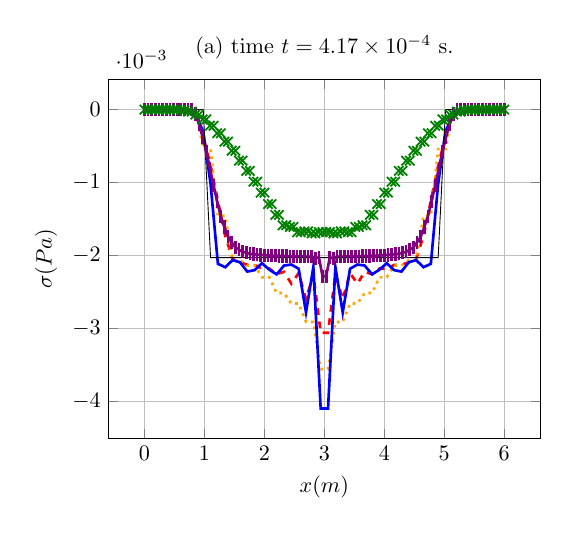
\begin{tikzpicture}[scale=0.8]
\begin{axis}[xlabel=$x (m)$,ylabel=$\sigma (Pa)$,ymajorgrids=true,xmajorgrids=true,legend pos=outer north east,title={(a) time $t = 4.17\times 10^{-4} $ s.}]
\addplot[Red,very thick,mark=none,dashed,mark size=3pt] coordinates {(0.0,0.0) (0.12244897959183673,0.0) (0.24489795918367346,0.0) (0.36734693877551017,0.0) (0.4897959183673469,0.0) (0.6122448979591837,0.0) (0.7346938775510203,0.0) (0.8571428571428571,-6.202478730418737e-05) (0.9795918367346939,-0.00036813096704147385) (1.1020408163265305,-0.0007691528823152809) (1.2244897959183674,-0.0012543541021143585) (1.346938775510204,-0.0017356166211235171) (1.4693877551020407,-0.002048755635913076) (1.5918367346938775,-0.002094430310096999) (1.7142857142857142,-0.0021297551418847207) (1.836734693877551,-0.0021313029263994436) (1.9591836734693877,-0.002184521512510678) (2.0816326530612246,-0.00218056135788198) (2.204081632653061,-0.002258201109747678) (2.326530612244898,-0.002225982674765895) (2.4489795918367347,-0.002388543727551356) (2.571428571428571,-0.002244426952247742) (2.693877551020408,-0.0026005478911843055) (2.816326530612245,-0.0022597626423764634) (2.9387755102040813,-0.003061428019909765) (3.061224489795918,-0.0030614280215042616) (3.183673469387755,-0.0022597625090894887) (3.306122448979592,-0.002600547891240036) (3.4285714285714284,-0.002244427149181305) (3.5510204081632653,-0.002388545096837233) (3.673469387755102,-0.0022259826134320305) (3.7959183673469385,-0.0022582009867140973) (3.9183673469387754,-0.002180561275761312) (4.040816326530612,-0.0021845214357378586) (4.163265306122449,-0.002131302759394598) (4.285714285714286,-0.002129755100625247) (4.408163265306122,-0.002094430313913873) (4.530612244897959,-0.0020487556136377133) (4.653061224489796,-0.0017356165629137574) (4.775510204081632,-0.0012543540420868722) (4.8979591836734695,-0.0007691528306923785) (5.020408163265306,-0.0003681309505408407) (5.142857142857142,-6.202478167641273e-05) (5.26530612244898,0.0) (5.387755102040816,0.0) (5.5102040816326525,0.0) (5.63265306122449,0.0) (5.755102040816326,0.0) (5.877551020408163,0.0) (6.0,0.0) };
\addplot[Orange,very thick,mark=none,dotted,mark size=3pt] coordinates {(0.0,0.0) (0.12244897959183673,0.0) (0.24489795918367346,0.0) (0.36734693877551017,0.0) (0.4897959183673469,0.0) (0.6122448979591837,0.0) (0.7346938775510203,0.0) (0.8571428571428571,0.0) (0.9795918367346939,-0.0005428735747303799) (1.1020408163265305,-0.0005428735744531341) (1.2244897959183674,-0.0014572018602302672) (1.346938775510204,-0.0014572015902572387) (1.4693877551020407,-0.0020650115628520543) (1.5918367346938775,-0.0020650115564237073) (1.7142857142857142,-0.002139129481636798) (1.836734693877551,-0.0021391292444730356) (1.9591836734693877,-0.0022996164460252094) (2.0816326530612246,-0.002299616288054982) (2.204081632653061,-0.002516346947664154) (2.326530612244898,-0.0025163468605162867) (2.4489795918367347,-0.002661476250005421) (2.571428571428571,-0.002661476165813169) (2.693877551020408,-0.002914184951969489) (2.816326530612245,-0.002914184944960401) (2.9387755102040813,-0.0035584423947308316) (3.061224489795918,-0.0035584423949992497) (3.183673469387755,-0.002914184951967428) (3.306122448979592,-0.0029141849534476782) (3.4285714285714284,-0.002661476845762277) (3.5510204081632653,-0.002661476777823057) (3.673469387755102,-0.0025163471827648032) (3.7959183673469385,-0.002516347115664522) (3.9183673469387754,-0.002299616671773065) (4.040816326530612,-0.0022996166084223715) (4.163265306122449,-0.002139129392056909) (4.285714285714286,-0.002139129375421892) (4.408163265306122,-0.002065011745290744) (4.530612244897959,-0.002065011751795016) (4.653061224489796,-0.001457201751052586) (4.775510204081632,-0.0014572017763862047) (4.8979591836734695,-0.000542873542473533) (5.020408163265306,-0.0005428735429029903) (5.142857142857142,0.0) (5.26530612244898,0.0) (5.387755102040816,0.0) (5.5102040816326525,0.0) (5.63265306122449,0.0) (5.755102040816326,0.0) (5.877551020408163,0.0) (6.0,0.0) };
\addplot[Blue,very thick,mark=none,solid,mark size=3pt] coordinates {(0.0,0.0) (0.12244897959183673,0.0) (0.24489795918367346,0.0) (0.36734693877551017,0.0) (0.4897959183673469,0.0) (0.6122448979591837,-6.278098647312321e-06) (0.7346938775510203,-2.4041734526500193e-05) (0.8571428571428571,-8.231252354464475e-05) (0.9795918367346939,-0.0002991596449725322) (1.1020408163265305,-0.0010179588589277829) (1.2244897959183674,-0.00211651125785778) (1.346938775510204,-0.002162627546957125) (1.4693877551020407,-0.002065078047300572) (1.5918367346938775,-0.0020946463817869327) (1.7142857142857142,-0.0022225969088509835) (1.836734693877551,-0.002202804765156386) (1.9591836734693877,-0.002108476200955529) (2.0816326530612246,-0.0021961061957235994) (2.204081632653061,-0.002260872273804215) (2.326530612244898,-0.0021401979709746418) (2.4489795918367347,-0.0021260586132198643) (2.571428571428571,-0.0021835117504344485) (2.693877551020408,-0.0027831455563594575) (2.816326530612245,-0.0021603089312707217) (2.9387755102040813,-0.00410115942266404) (3.061224489795918,-0.00410115942266404) (3.183673469387755,-0.0021603089312707195) (3.306122448979592,-0.0027831455563594575) (3.4285714285714284,-0.0021835117504344498) (3.5510204081632653,-0.0021260586132198643) (3.673469387755102,-0.0021401979709746426) (3.7959183673469385,-0.002260872273804217) (3.9183673469387754,-0.0021961061957235903) (4.040816326530612,-0.002108476200955527) (4.163265306122449,-0.002202804765156385) (4.285714285714286,-0.002222596908850955) (4.408163265306122,-0.00209464638178693) (4.530612244897959,-0.002065078047300569) (4.653061224489796,-0.0021626275469571166) (4.775510204081632,-0.0021165112578577674) (4.8979591836734695,-0.0010179588589277811) (5.020408163265306,-0.0002991596449725306) (5.142857142857142,-8.231252354464585e-05) (5.26530612244898,-2.404173452650139e-05) (5.387755102040816,-6.278098647312686e-06) (5.5102040816326525,0.0) (5.63265306122449,0.0) (5.755102040816326,0.0) (5.877551020408163,0.0) (6.0,0.0) };
\addplot[Purple,very thick,mark=|,solid,mark size=3pt] coordinates {(0.0,0.0) (0.06060606060606061,0.0) (0.12121212121212122,0.0) (0.18181818181818182,0.0) (0.24242424242424243,0.0) (0.30303030303030304,0.0) (0.36363636363636365,0.0) (0.42424242424242425,0.0) (0.48484848484848486,0.0) (0.5454545454545454,0.0) (0.6060606060606061,0.0) (0.6666666666666667,0.0) (0.7272727272727273,0.0) (0.7878787878787878,-2.102087026510683e-10) (0.8484848484848485,-5.933454445134857e-05) (0.9090909090909092,-0.00019666441211383344) (0.9696969696969697,-0.000374409291697533) (1.0303030303030303,-0.0005722648866595782) (1.0909090909090908,-0.0008056893472495531) (1.1515151515151516,-0.001039344553408203) (1.2121212121212122,-0.0012582426511154375) (1.2727272727272727,-0.001463343679322638) (1.3333333333333335,-0.0016127307863671309) (1.393939393939394,-0.0017460505019539665) (1.4545454545454546,-0.0018218179515133914) (1.5151515151515151,-0.0018898271010591291) (1.5757575757575757,-0.0019212706379672865) (1.6363636363636365,-0.0019517753164705633) (1.696969696969697,-0.0019640200241847683) (1.7575757575757576,-0.0019777892349964947) (1.8181818181818183,-0.00198321411930953) (1.878787878787879,-0.0019904956763223034) (1.9393939393939394,-0.001993427920769702) (2.0,-0.0019980258450979097) (2.0606060606060606,-0.0019998696750316023) (2.121212121212121,-0.002003218730140839) (2.1818181818181817,-0.002004470567368423) (2.2424242424242427,-0.0020071540285014795) (2.303030303030303,-0.002007999665063322) (2.3636363636363638,-0.00201032098232525) (2.4242424242424243,-0.0020108541583820755) (2.484848484848485,-0.0020131468962690698) (2.5454545454545454,-0.0020134626237766347) (2.606060606060606,-0.0020161438749334505) (2.666666666666667,-0.002016134393902099) (2.7272727272727275,-0.00201958433697188) (2.787878787878788,-0.0020188214892157487) (2.8484848484848486,-0.0020416792740526437) (2.909090909090909,-0.002026433031381828) (2.9696969696969697,-0.0022869057829180586) (3.0303030303030303,-0.0022869057829180586) (3.090909090909091,-0.00202643303138183) (3.1515151515151514,-0.0020416792740526424) (3.2121212121212124,-0.0020188214892157483) (3.272727272727273,-0.002019584336971879) (3.3333333333333335,-0.0020161343939021) (3.393939393939394,-0.002016143874933451) (3.4545454545454546,-0.002013462623776635) (3.515151515151515,-0.0020131468962690698) (3.5757575757575757,-0.0020108541583820755) (3.6363636363636367,-0.00201032098232525) (3.6969696969696972,-0.0020079996650633225) (3.757575757575758,-0.00200715402850148) (3.8181818181818183,-0.0020044705673684248) (3.878787878787879,-0.002003218730140839) (3.9393939393939394,-0.001999869675031603) (4.0,-0.0019980258450979105) (4.0606060606060606,-0.001993427920769704) (4.121212121212121,-0.0019904956763223043) (4.181818181818182,-0.0019832141193095324) (4.242424242424242,-0.001977789234996496) (4.303030303030303,-0.0019640200241847713) (4.363636363636363,-0.0019517753164705652) (4.424242424242425,-0.001921270637967289) (4.484848484848485,-0.0018898271010591296) (4.545454545454546,-0.001821817951513394) (4.606060606060606,-0.0017460505019539676) (4.666666666666667,-0.0016127307863671332) (4.7272727272727275,-0.001463343679322639) (4.787878787878788,-0.001258242651115441) (4.848484848484849,-0.0010393445534082066) (4.909090909090909,-0.0008056893472495551) (4.96969696969697,-0.0005722648866595818) (5.03030303030303,-0.00037440929169753735) (5.090909090909091,-0.0001966644121138361) (5.151515151515151,-5.933454445134941e-05) (5.212121212121212,-2.1020870265128841e-10) (5.2727272727272725,0.0) (5.333333333333334,0.0) (5.3939393939393945,0.0) (5.454545454545455,0.0) (5.515151515151516,0.0) (5.575757575757576,0.0) (5.636363636363637,0.0) (5.696969696969697,0.0) (5.757575757575758,0.0) (5.818181818181818,0.0) (5.878787878787879,0.0) (5.9393939393939394,0.0) (6.0,0.0) };
\addplot[Green,thick,mark=x,only marks,mark size=3pt] coordinates {(0.0,0.0) (0.06060606060606061,0.0) (0.12121212121212122,0.0) (0.18181818181818182,0.0) (0.24242424242424243,0.0) (0.30303030303030304,0.0) (0.36363636363636365,0.0) (0.42424242424242425,0.0) (0.48484848484848486,0.0) (0.5454545454545454,0.0) (0.6060606060606061,-7.541928868240051e-06) (0.6666666666666667,-7.541928868229345e-06) (0.7272727272727273,-2.7084017957293276e-05) (0.7878787878787878,-2.7084017957300184e-05) (0.8484848484848485,-6.859713739037666e-05) (0.9090909090909092,-6.859713739037584e-05) (0.9696969696969697,-0.0001344887591217594) (1.0303030303030303,-0.00013448875912177324) (1.0909090909090908,-0.00022152236877268994) (1.1515151515151516,-0.00022152236877268793) (1.2121212121212122,-0.0003242523797458477) (1.2727272727272727,-0.0003242523797458495) (1.3333333333333335,-0.0004401175241166998) (1.393939393939394,-0.0004401175241166955) (1.4545454545454546,-0.0005652783736503705) (1.5151515151515151,-0.0005652783736503665) (1.5757575757575757,-0.0007004668759840085) (1.6363636363636365,-0.0007004668759840094) (1.696969696969697,-0.0008407298830150507) (1.7575757575757576,-0.0008407298830150555) (1.8181818181818183,-0.0009896799388507634) (1.878787878787879,-0.0009896799388507537) (1.9393939393939394,-0.0011394881053837696) (2.0,-0.0011394881053837483) (2.0606060606060606,-0.0012962218995730156) (2.121212121212121,-0.001296221899573015) (2.1818181818181817,-0.0014442461283461112) (2.2424242424242427,-0.0014442461283460791) (2.303030303030303,-0.0015870213580057504) (2.3636363636363638,-0.0015870213580057664) (2.4242424242424243,-0.001609952015030185) (2.484848484848485,-0.0016099520150300688) (2.5454545454545454,-0.0016826381193043032) (2.606060606060606,-0.0016826381193043207) (2.666666666666667,-0.0016712124587595317) (2.7272727272727275,-0.0016712124587595961) (2.787878787878788,-0.0016984318779487367) (2.8484848484848486,-0.0016984318779487292) (2.909090909090909,-0.0016803916060842941) (2.9696969696969697,-0.0016803916060843564) (3.0303030303030303,-0.0016803916060841846) (3.090909090909091,-0.0016803916060842375) (3.1515151515151514,-0.0016984318779488911) (3.2121212121212124,-0.001698431877948936) (3.272727272727273,-0.0016712124587594489) (3.3333333333333335,-0.0016712124587594413) (3.393939393939394,-0.0016826381193042644) (3.4545454545454546,-0.0016826381193042119) (3.515151515151515,-0.001609952015029999) (3.5757575757575757,-0.0016099520150300668) (3.6363636363636367,-0.0015870213580056888) (3.6969696969696972,-0.0015870213580057126) (3.757575757575758,-0.0014442461283460722) (3.8181818181818183,-0.001444246128346086) (3.878787878787879,-0.0012962218995730295) (3.9393939393939394,-0.0012962218995730172) (4.0,-0.0011394881053837505) (4.0606060606060606,-0.0011394881053837492) (4.121212121212121,-0.000989679938850742) (4.181818181818182,-0.0009896799388507615) (4.242424242424242,-0.0008407298830150445) (4.303030303030303,-0.0008407298830150564) (4.363636363636363,-0.0007004668759840193) (4.424242424242425,-0.0007004668759840206) (4.484848484848485,-0.0005652783736503635) (4.545454545454546,-0.0005652783736503715) (4.606060606060606,-0.0004401175241167171) (4.666666666666667,-0.0004401175241167155) (4.7272727272727275,-0.00032425237974587187) (4.787878787878788,-0.0003242523797458809) (4.848484848484849,-0.00022152236877269233) (4.909090909090909,-0.00022152236877269926) (4.96969696969697,-0.00013448875912178598) (5.03030303030303,-0.0001344887591217872) (5.090909090909091,-6.859713739045158e-05) (5.151515151515151,-6.859713739045805e-05) (5.212121212121212,-2.7084017957307516e-05) (5.2727272727272725,-2.708401795731454e-05) (5.333333333333334,-7.541928868230607e-06) (5.3939393939393945,-7.541928868233546e-06) (5.454545454545455,0.0) (5.515151515151516,0.0) (5.575757575757576,0.0) (5.636363636363637,0.0) (5.696969696969697,0.0) (5.757575757575758,0.0) (5.818181818181818,0.0) (5.878787878787879,0.0) (5.9393939393939394,0.0) (6.0,0.0) };
\addplot[black,thin,mark=none,solid,mark size=3pt] coordinates {(0.0,-0.0) (0.12244897959183673,-0.0) (0.24489795918367346,-0.0) (0.36734693877551017,-0.0) (0.4897959183673469,-0.0) (0.6122448979591837,-0.0) (0.7346938775510203,-0.0) (0.8571428571428571,-0.0) (0.9795918367346939,-0.0) (1.1020408163265305,-0.002030785796418313) (1.2244897959183674,-0.002030785796418313) (1.346938775510204,-0.002030785796418313) (1.4693877551020407,-0.002030785796418313) (1.5918367346938775,-0.002030785796418313) (1.7142857142857142,-0.002030785796418313) (1.836734693877551,-0.002030785796418313) (1.9591836734693877,-0.002030785796418313) (2.0816326530612246,-0.002030785796418313) (2.204081632653061,-0.002030785796418313) (2.326530612244898,-0.002030785796418313) (2.4489795918367347,-0.002030785796418313) (2.571428571428571,-0.002030785796418313) (2.693877551020408,-0.002030785796418313) (2.816326530612245,-0.002030785796418313) (2.9387755102040813,-0.002030785796418313) (3.061224489795918,-0.002030785796418313) (3.183673469387755,-0.002030785796418313) (3.306122448979592,-0.002030785796418313) (3.4285714285714284,-0.002030785796418313) (3.5510204081632653,-0.002030785796418313) (3.673469387755102,-0.002030785796418313) (3.7959183673469385,-0.002030785796418313) (3.9183673469387754,-0.002030785796418313) (4.040816326530612,-0.002030785796418313) (4.163265306122449,-0.002030785796418313) (4.285714285714286,-0.002030785796418313) (4.408163265306122,-0.002030785796418313) (4.530612244897959,-0.002030785796418313) (4.653061224489796,-0.002030785796418313) (4.775510204081632,-0.002030785796418313) (4.8979591836734695,-0.002030785796418313) (5.020408163265306,-0.0) (5.142857142857142,-0.0) (5.26530612244898,-0.0) (5.387755102040816,-0.0) (5.5102040816326525,-0.0) (5.63265306122449,-0.0) (5.755102040816326,-0.0) (5.877551020408163,-0.0) (6.0,-0.0) };
%\legend{usl 1ppc,usf 1ppc,dgmpm 1ppc,dgmpm 2ppc,dgmpm 2ppc (RK2 + strang),plastic solution}
\end{axis}
\end{tikzpicture}
%%% Local Variables:
%%% mode: latex
%%% TeX-master: "../../mainManuscript"
%%% End:
}
%   {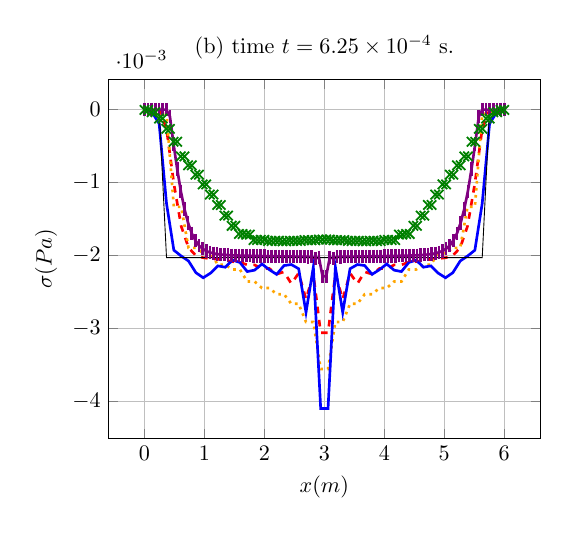
\begin{tikzpicture}[scale=0.8]
\begin{axis}[xlabel=$x (m)$,ylabel=$\sigma (Pa)$,ymajorgrids=true,xmajorgrids=true,legend pos=outer north east,title={(b) time $t = 6.25\times 10^{-4} $ s.}]
\addplot[Red,very thick,mark=none,dashed,mark size=3pt] coordinates {(0.0,0.0) (0.12244897959183673,0.0) (0.24489795918367346,0.0) (0.36734693877551017,-0.00026483849578394367) (0.4897959183673469,-0.001013521443045474) (0.6122448979591837,-0.001599418396582166) (0.7346938775510203,-0.001894897583975942) (0.8571428571428571,-0.002003175763253103) (0.9795918367346939,-0.0020325617224383253) (1.1020408163265305,-0.002045228028080732) (1.2244897959183674,-0.002053732290291538) (1.346938775510204,-0.002068698427659408) (1.4693877551020407,-0.002085802417563694) (1.5918367346938775,-0.002094430310096999) (1.7142857142857142,-0.0021297551418847207) (1.836734693877551,-0.0021313029263994436) (1.9591836734693877,-0.002184521512510678) (2.0816326530612246,-0.00218056135788198) (2.204081632653061,-0.002258201109747678) (2.326530612244898,-0.002225982674765895) (2.4489795918367347,-0.002388543727551356) (2.571428571428571,-0.002244426952247742) (2.693877551020408,-0.0026005478911843055) (2.816326530612245,-0.0022597626423764634) (2.9387755102040813,-0.003061428019909765) (3.061224489795918,-0.0030614280215042616) (3.183673469387755,-0.0022597625090894887) (3.306122448979592,-0.002600547891240036) (3.4285714285714284,-0.002244427149181305) (3.5510204081632653,-0.002388545096837233) (3.673469387755102,-0.0022259826134320305) (3.7959183673469385,-0.0022582009867140973) (3.9183673469387754,-0.002180561275761312) (4.040816326530612,-0.0021845214357378586) (4.163265306122449,-0.002131302759394598) (4.285714285714286,-0.002129755100625247) (4.408163265306122,-0.002094430313913873) (4.530612244897959,-0.002085802281263282) (4.653061224489796,-0.0020686990340733047) (4.775510204081632,-0.002053732101494861) (4.8979591836734695,-0.002045227646988374) (5.020408163265306,-0.002032561293211891) (5.142857142857142,-0.002003175773545243) (5.26530612244898,-0.001894903223389431) (5.387755102040816,-0.0015994182857342976) (5.5102040816326525,-0.0010135213099064534) (5.63265306122449,-0.0002648400904681731) (5.755102040816326,0.0) (5.877551020408163,0.0) (6.0,0.0) };
\addplot[Orange,very thick,mark=none,dotted,mark size=3pt] coordinates {(0.0,0.0) (0.12244897959183673,0.0) (0.24489795918367346,-5.7301755105765905e-05) (0.36734693877551017,-5.730189455576938e-05) (0.4897959183673469,-0.0013347906501971517) (0.6122448979591837,-0.0013347901679111186) (0.7346938775510203,-0.0018978853621068183) (0.8571428571428571,-0.0018978850318875267) (0.9795918367346939,-0.0019688602343015333) (1.1020408163265305,-0.001968859643255841) (1.2244897959183674,-0.0021294179293388526) (1.346938775510204,-0.0021294183868218043) (1.4693877551020407,-0.002194450786388116) (1.5918367346938775,-0.002194450017072264) (1.7142857142857142,-0.002359628639203141) (1.836734693877551,-0.002359632498979967) (1.9591836734693877,-0.0024482611380392057) (2.0816326530612246,-0.0024482617498292327) (2.204081632653061,-0.0025330451235017004) (2.326530612244898,-0.0025330454201282796) (2.4489795918367347,-0.0026644433282951813) (2.571428571428571,-0.002664443159431375) (2.693877551020408,-0.002914184951969489) (2.816326530612245,-0.002914184944960401) (2.9387755102040813,-0.0035584423947308316) (3.061224489795918,-0.0035584423949992497) (3.183673469387755,-0.002914184951967428) (3.306122448979592,-0.0029141849534476782) (3.4285714285714284,-0.002664444198988343) (3.5510204081632653,-0.002664443841077106) (3.673469387755102,-0.0025330448069917346) (3.7959183673469385,-0.002533045701171117) (3.9183673469387754,-0.002448256452448852) (4.040816326530612,-0.002448261928651275) (4.163265306122449,-0.0023596324432405987) (4.285714285714286,-0.0023596329747803267) (4.408163265306122,-0.002194450734585246) (4.530612244897959,-0.002194449738710537) (4.653061224489796,-0.0021294183668896256) (4.775510204081632,-0.002129418349055579) (4.8979591836734695,-0.001968860118219393) (5.020408163265306,-0.0019688594313722226) (5.142857142857142,-0.0018978854498614389) (5.26530612244898,-0.0018978851381802133) (5.387755102040816,-0.0013347904245097116) (5.5102040816326525,-0.001334790188952414) (5.63265306122449,-5.730185243339023e-05) (5.755102040816326,-5.730185485343143e-05) (5.877551020408163,0.0) (6.0,0.0) };
\addplot[Blue,very thick,mark=none,solid,mark size=3pt] coordinates {(0.0,-3.893079067418818e-06) (0.12244897959183673,-3.047957003773611e-05) (0.24489795918367346,-0.000194336720102431) (0.36734693877551017,-0.0012876041625046832) (0.4897959183673469,-0.0019289954950223976) (0.6122448979591837,-0.002009227173232224) (0.7346938775510203,-0.0020777863701164022) (0.8571428571428571,-0.0022375987292720654) (0.9795918367346939,-0.0023072199656024722) (1.1020408163265305,-0.002243560529202433) (1.2244897959183674,-0.0021445098783626536) (1.346938775510204,-0.002162627546957125) (1.4693877551020407,-0.002065314702320964) (1.5918367346938775,-0.0020976556349240846) (1.7142857142857142,-0.0022225969088509835) (1.836734693877551,-0.0022028059756579103) (1.9591836734693877,-0.002118543769523527) (2.0816326530612246,-0.0021961061957235994) (2.204081632653061,-0.002260872273804215) (2.326530612244898,-0.0021401979709746418) (2.4489795918367347,-0.0021260586132198643) (2.571428571428571,-0.0021835117504344485) (2.693877551020408,-0.0027831455563594575) (2.816326530612245,-0.0021603089312707217) (2.9387755102040813,-0.00410115942266404) (3.061224489795918,-0.00410115942266404) (3.183673469387755,-0.0021603089312707195) (3.306122448979592,-0.0027831455563594575) (3.4285714285714284,-0.0021835117504344498) (3.5510204081632653,-0.0021260586132198643) (3.673469387755102,-0.0021401979709746426) (3.7959183673469385,-0.002260872273804217) (3.9183673469387754,-0.0021961061957235903) (4.040816326530612,-0.002118543769523527) (4.163265306122449,-0.002202805975657909) (4.285714285714286,-0.002222596908850955) (4.408163265306122,-0.0020976556349240833) (4.530612244897959,-0.0020653147023209618) (4.653061224489796,-0.0021626275469571166) (4.775510204081632,-0.0021445098783626554) (4.8979591836734695,-0.002243560529202434) (5.020408163265306,-0.002307219965602473) (5.142857142857142,-0.0022375987292720598) (5.26530612244898,-0.002077786370116406) (5.387755102040816,-0.002009227173232226) (5.5102040816326525,-0.0019289954950223924) (5.63265306122449,-0.0012876041625046687) (5.755102040816326,-0.00019433672010243214) (5.877551020408163,-3.047957003773766e-05) (6.0,-3.89307906741869e-06) };
\addplot[Purple,very thick,mark=|,solid,mark size=3pt] coordinates {(0.0,0.0) (0.06060606060606061,0.0) (0.12121212121212122,0.0) (0.18181818181818182,0.0) (0.24242424242424243,0.0) (0.30303030303030304,0.0) (0.36363636363636365,0.0) (0.42424242424242425,-9.478454557786464e-05) (0.48484848484848486,-0.0004733763203636077) (0.5454545454545454,-0.000814341803859037) (0.6060606060606061,-0.00111922644858282) (0.6666666666666667,-0.0013639777840079603) (0.7272727272727273,-0.0015544317104102714) (0.7878787878787878,-0.0016969397043999374) (0.8484848484848485,-0.0017949331499141452) (0.9090909090909092,-0.0018654199222256865) (0.9696969696969697,-0.0019091603206922254) (1.0303030303030303,-0.0019406187410981471) (1.0909090909090908,-0.0019590334022499775) (1.1515151515151516,-0.001973016484643746) (1.2121212121212122,-0.0019812974809459826) (1.2727272727272727,-0.0019882165408146835) (1.3333333333333335,-0.001992517920818215) (1.393939393939394,-0.00199644892142901) (1.4545454545454546,-0.001998847531766857) (1.5151515151515151,-0.0020012976353965943) (1.5757575757575757,-0.002002723340276947) (1.6363636363636365,-0.0020044767003141563) (1.696969696969697,-0.002005455954611059) (1.7575757575757576,-0.0020068717566027695) (1.8181818181818183,-0.0020076243914485758) (1.878787878787879,-0.0020088510479386633) (1.9393939393939394,-0.0020094619562297344) (2.0,-0.0020105817510746183) (2.0606060606060606,-0.002011097015992123) (2.121212121212121,-0.0020121761338987108) (2.1818181818181817,-0.0020126171467676774) (2.2424242424242427,-0.0020136968548150214) (2.303030303030303,-0.0020140562994433687) (2.3636363636363638,-0.002015172057998995) (2.4242424242424243,-0.0020154349921928374) (2.484848484848485,-0.0020167112186900084) (2.5454545454545454,-0.002016887611422729) (2.606060606060606,-0.0020185925173496996) (2.666666666666667,-0.002018578059346721) (2.7272727272727275,-0.002021063173066831) (2.787878787878788,-0.0020204807134743753) (2.8484848484848486,-0.0020416794860022825) (2.909090909090909,-0.002026827362087739) (2.9696969696969697,-0.0022869057829180586) (3.0303030303030303,-0.0022869057829180586) (3.090909090909091,-0.002026827362087741) (3.1515151515151514,-0.002041679486002281) (3.2121212121212124,-0.0020204807134743753) (3.272727272727273,-0.0020210631730668296) (3.3333333333333335,-0.0020185780593467225) (3.393939393939394,-0.0020185925173497004) (3.4545454545454546,-0.0020168876114227295) (3.515151515151515,-0.002016711218690009) (3.5757575757575757,-0.002015434992192838) (3.6363636363636367,-0.0020151720579989953) (3.6969696969696972,-0.002014056299443369) (3.757575757575758,-0.0020136968548150227) (3.8181818181818183,-0.002012617146767679) (3.878787878787879,-0.0020121761338987108) (3.9393939393939394,-0.002011097015992124) (4.0,-0.002010581751074619) (4.0606060606060606,-0.0020094619562297353) (4.121212121212121,-0.0020088510479386638) (4.181818181818182,-0.002007624391448577) (4.242424242424242,-0.00200687175660277) (4.303030303030303,-0.002005455954611061) (4.363636363636363,-0.0020044767003141568) (4.424242424242425,-0.0020027233402769486) (4.484848484848485,-0.002001297635396595) (4.545454545454546,-0.0019988475317668586) (4.606060606060606,-0.0019964489214290117) (4.666666666666667,-0.0019925179208182173) (4.7272727272727275,-0.0019882165408146857) (4.787878787878788,-0.0019812974809459843) (4.848484848484849,-0.0019730164846437476) (4.909090909090909,-0.0019590334022499805) (4.96969696969697,-0.0019406187410981489) (5.03030303030303,-0.0019091603206922276) (5.090909090909091,-0.001865419922225688) (5.151515151515151,-0.0017949331499141465) (5.212121212121212,-0.0016969397043999379) (5.2727272727272725,-0.0015544317104102714) (5.333333333333334,-0.0013639777840079614) (5.3939393939393945,-0.0011192264485828216) (5.454545454545455,-0.0008143418038590386) (5.515151515151516,-0.0004733763203636097) (5.575757575757576,-9.478454557786505e-05) (5.636363636363637,0.0) (5.696969696969697,0.0) (5.757575757575758,0.0) (5.818181818181818,0.0) (5.878787878787879,0.0) (5.9393939393939394,0.0) (6.0,0.0) };
\addplot[Green,thick,mark=x,only marks,mark size=3pt] coordinates {(0.0,-4.653556676445113e-06) (0.06060606060606061,-4.653556676466522e-06) (0.12121212121212122,-3.553597365446572e-05) (0.18181818181818182,-3.553597365448185e-05) (0.24242424242424243,-0.00012281470180235295) (0.30303030303030304,-0.00012281470180237252) (0.36363636363636365,-0.00026409308529461167) (0.42424242424242425,-0.0002640930852946001) (0.48484848484848486,-0.00044103089416509117) (0.5454545454545454,-0.0004410308941650814) (0.6060606060606061,-0.000641965342651722) (0.6666666666666667,-0.0006419653426517044) (0.7272727272727273,-0.0007642218788261203) (0.7878787878787878,-0.000764221878826115) (0.8484848484848485,-0.0008928462121140367) (0.9090909090909092,-0.0008928462121140418) (0.9696969696969697,-0.0010267020703216654) (1.0303030303030303,-0.0010267020703216743) (1.0909090909090908,-0.0011658963775695353) (1.1515151515151516,-0.0011658963775695475) (1.2121212121212122,-0.0013084847600696925) (1.2727272727272727,-0.0013084847600697092) (1.3333333333333335,-0.0014547578806386335) (1.393939393939394,-0.001454757880638625) (1.4545454545454546,-0.0015944875452197276) (1.5151515151515151,-0.0015944875452197434) (1.5757575757575757,-0.001707074178639678) (1.6363636363636365,-0.0017070741786396851) (1.696969696969697,-0.0017150623709443888) (1.7575757575757576,-0.001715062370944398) (1.8181818181818183,-0.001790298875206909) (1.878787878787879,-0.0017902988752067975) (1.9393939393939394,-0.0017871999380725328) (2.0,-0.0017871999380725146) (2.0606060606060606,-0.0018039003213189228) (2.121212121212121,-0.0018039003213188086) (2.1818181818181817,-0.0018002331089720413) (2.2424242424242427,-0.0018002331089720298) (2.303030303030303,-0.0018066356526349138) (2.3636363636363638,-0.001806635652634928) (2.4242424242424243,-0.0018005119579068544) (2.484848484848485,-0.001800511957906827) (2.5454545454545454,-0.0018027419309853173) (2.606060606060606,-0.001802741930985315) (2.666666666666667,-0.0017908982789932382) (2.7272727272727275,-0.0017908982789932527) (2.787878787878788,-0.0017920432553689817) (2.8484848484848486,-0.0017920432553690704) (2.909090909090909,-0.0017832541467531172) (2.9696969696969697,-0.001783254146753207) (3.0303030303030303,-0.0017832541467531968) (3.090909090909091,-0.0017832541467532597) (3.1515151515151514,-0.001792043255369177) (3.2121212121212124,-0.001792043255369262) (3.272727272727273,-0.0017908982789931235) (3.3333333333333335,-0.0017908982789931267) (3.393939393939394,-0.0018027419309851842) (3.4545454545454546,-0.00180274193098518) (3.515151515151515,-0.0018005119579067273) (3.5757575757575757,-0.0018005119579067206) (3.6363636363636367,-0.0018066356526347171) (3.6969696969696972,-0.001806635652634705) (3.757575757575758,-0.0018002331089718607) (3.8181818181818183,-0.0018002331089718572) (3.878787878787879,-0.0018039003213187017) (3.9393939393939394,-0.0018039003213188207) (4.0,-0.0017871999380728316) (4.0606060606060606,-0.001787199938072803) (4.121212121212121,-0.0017902988752070415) (4.181818181818182,-0.001790298875207153) (4.242424242424242,-0.0017150623709445087) (4.303030303030303,-0.0017150623709445115) (4.363636363636363,-0.001707074178639759) (4.424242424242425,-0.0017070741786397732) (4.484848484848485,-0.0015944875452197688) (4.545454545454546,-0.0015944875452197464) (4.606060606060606,-0.0014547578806386077) (4.666666666666667,-0.0014547578806386094) (4.7272727272727275,-0.0013084847600697066) (4.787878787878788,-0.0013084847600697033) (4.848484848484849,-0.0011658963775695345) (4.909090909090909,-0.0011658963775695356) (4.96969696969697,-0.001026702070321666) (5.03030303030303,-0.0010267020703216456) (5.090909090909091,-0.0008928462121140489) (5.151515151515151,-0.0008928462121140479) (5.212121212121212,-0.0007642218788261214) (5.2727272727272725,-0.0007642218788261214) (5.333333333333334,-0.0006419653426517155) (5.3939393939393945,-0.0006419653426517138) (5.454545454545455,-0.000441030894165099) (5.515151515151516,-0.0004410308941651111) (5.575757575757576,-0.00026409308529464273) (5.636363636363637,-0.0002640930852946408) (5.696969696969697,-0.0001228147018024683) (5.757575757575758,-0.0001228147018024451) (5.818181818181818,-3.553597365452076e-05) (5.878787878787879,-3.553597365451883e-05) (5.9393939393939394,-4.653556676452633e-06) (6.0,-4.653556676488362e-06) };
\addplot[black,thin,mark=none,solid,mark size=3pt] coordinates {(0.0,-0.0) (0.12244897959183673,-0.0) (0.24489795918367346,-0.0) (0.36734693877551017,-0.002030785796418313) (0.4897959183673469,-0.002030785796418313) (0.6122448979591837,-0.002030785796418313) (0.7346938775510203,-0.002030785796418313) (0.8571428571428571,-0.002030785796418313) (0.9795918367346939,-0.002030785796418313) (1.1020408163265305,-0.002030785796418313) (1.2244897959183674,-0.002030785796418313) (1.346938775510204,-0.002030785796418313) (1.4693877551020407,-0.002030785796418313) (1.5918367346938775,-0.002030785796418313) (1.7142857142857142,-0.002030785796418313) (1.836734693877551,-0.002030785796418313) (1.9591836734693877,-0.002030785796418313) (2.0816326530612246,-0.002030785796418313) (2.204081632653061,-0.002030785796418313) (2.326530612244898,-0.002030785796418313) (2.4489795918367347,-0.002030785796418313) (2.571428571428571,-0.002030785796418313) (2.693877551020408,-0.002030785796418313) (2.816326530612245,-0.002030785796418313) (2.9387755102040813,-0.002030785796418313) (3.061224489795918,-0.002030785796418313) (3.183673469387755,-0.002030785796418313) (3.306122448979592,-0.002030785796418313) (3.4285714285714284,-0.002030785796418313) (3.5510204081632653,-0.002030785796418313) (3.673469387755102,-0.002030785796418313) (3.7959183673469385,-0.002030785796418313) (3.9183673469387754,-0.002030785796418313) (4.040816326530612,-0.002030785796418313) (4.163265306122449,-0.002030785796418313) (4.285714285714286,-0.002030785796418313) (4.408163265306122,-0.002030785796418313) (4.530612244897959,-0.002030785796418313) (4.653061224489796,-0.002030785796418313) (4.775510204081632,-0.002030785796418313) (4.8979591836734695,-0.002030785796418313) (5.020408163265306,-0.002030785796418313) (5.142857142857142,-0.002030785796418313) (5.26530612244898,-0.002030785796418313) (5.387755102040816,-0.002030785796418313) (5.5102040816326525,-0.002030785796418313) (5.63265306122449,-0.002030785796418313) (5.755102040816326,-0.0) (5.877551020408163,-0.0) (6.0,-0.0) };
%\legend{usl 1ppc,usf 1ppc,dgmpm 1ppc,dgmpm 2ppc,dgmpm 2ppc (RK2 + strang),plastic solution}
\end{axis}
\end{tikzpicture}
%%% Local Variables:
%%% mode: latex
%%% TeX-master: "../../mainManuscript"
%%% End:
}
%   {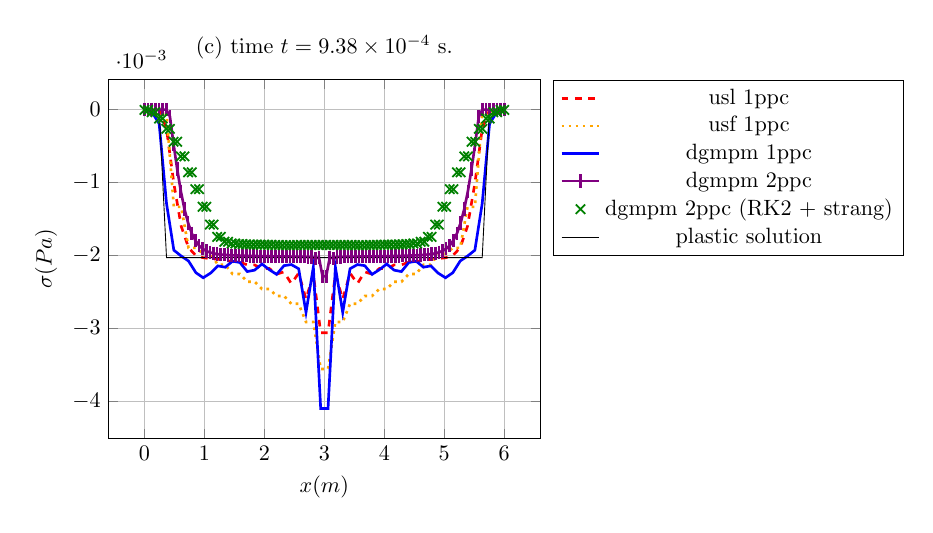
\begin{tikzpicture}[scale=0.8]
\begin{axis}[xlabel=$x (m)$,ylabel=$\sigma (Pa)$,ymajorgrids=true,xmajorgrids=true,legend pos=outer north east,title={(c) time $t = 9.38\times 10^{-4} $ s.}]
\addplot[Red,very thick,mark=none,dashed,mark size=3pt] coordinates {(0.0,0.0) (0.12244897959183673,0.0) (0.24489795918367346,0.0) (0.36734693877551017,-0.00026483849578394367) (0.4897959183673469,-0.001013521443045474) (0.6122448979591837,-0.001599418396582166) (0.7346938775510203,-0.001894897583975942) (0.8571428571428571,-0.002003175763253103) (0.9795918367346939,-0.0020325617224383253) (1.1020408163265305,-0.002045228028080732) (1.2244897959183674,-0.002053732290291538) (1.346938775510204,-0.002068698427659408) (1.4693877551020407,-0.002085802417563694) (1.5918367346938775,-0.002094430310096999) (1.7142857142857142,-0.0021297551418847207) (1.836734693877551,-0.0021313029263994436) (1.9591836734693877,-0.002184521512510678) (2.0816326530612246,-0.00218056135788198) (2.204081632653061,-0.002258201109747678) (2.326530612244898,-0.002225982674765895) (2.4489795918367347,-0.002388543727551356) (2.571428571428571,-0.002244426952247742) (2.693877551020408,-0.0026005478911843055) (2.816326530612245,-0.0022597626423764634) (2.9387755102040813,-0.003061428019909765) (3.061224489795918,-0.0030614280215042616) (3.183673469387755,-0.0022597625090894887) (3.306122448979592,-0.002600547891240036) (3.4285714285714284,-0.002244427149181305) (3.5510204081632653,-0.002388545096837233) (3.673469387755102,-0.0022259826134320305) (3.7959183673469385,-0.0022582009867140973) (3.9183673469387754,-0.002180561275761312) (4.040816326530612,-0.0021845214357378586) (4.163265306122449,-0.002131302759394598) (4.285714285714286,-0.002129755100625247) (4.408163265306122,-0.002094430313913873) (4.530612244897959,-0.002085802281263282) (4.653061224489796,-0.0020686990340733047) (4.775510204081632,-0.002053732101494861) (4.8979591836734695,-0.002045227646988374) (5.020408163265306,-0.002032561293211891) (5.142857142857142,-0.002003175773545243) (5.26530612244898,-0.001894903223389431) (5.387755102040816,-0.0015994182857342976) (5.5102040816326525,-0.0010135213099064534) (5.63265306122449,-0.0002648400904681731) (5.755102040816326,0.0) (5.877551020408163,0.0) (6.0,0.0) };
\addplot[Orange,very thick,mark=none,dotted,mark size=3pt] coordinates {(0.0,0.0) (0.12244897959183673,0.0) (0.24489795918367346,-5.7301755105765905e-05) (0.36734693877551017,-5.730189455576938e-05) (0.4897959183673469,-0.0013347906501971517) (0.6122448979591837,-0.0013347901679111186) (0.7346938775510203,-0.0018978853621068183) (0.8571428571428571,-0.0018978850318875267) (0.9795918367346939,-0.0019799715434199354) (1.1020408163265305,-0.0019799696050827615) (1.2244897959183674,-0.0021294179293388526) (1.346938775510204,-0.0021294183868218043) (1.4693877551020407,-0.002255946410111241) (1.5918367346938775,-0.0022559455216042603) (1.7142857142857142,-0.0023619885239961427) (1.836734693877551,-0.002361991742698304) (1.9591836734693877,-0.0024610525543925722) (2.0816326530612246,-0.0024610535623674854) (2.204081632653061,-0.0025567250194484252) (2.326530612244898,-0.002556724888093118) (2.4489795918367347,-0.002664443582915471) (2.571428571428571,-0.002664443413600718) (2.693877551020408,-0.002914184951969489) (2.816326530612245,-0.002914184944960401) (2.9387755102040813,-0.0035584423947308316) (3.061224489795918,-0.0035584423949992497) (3.183673469387755,-0.002914184951967428) (3.306122448979592,-0.0029141849534476782) (3.4285714285714284,-0.0026644444535014193) (3.5510204081632653,-0.0026644440952976736) (3.673469387755102,-0.0025567222026880295) (3.7959183673469385,-0.002556725323601323) (3.9183673469387754,-0.0024610504976733446) (4.040816326530612,-0.0024610474461122947) (4.163265306122449,-0.002361991399376669) (4.285714285714286,-0.0023619921199265104) (4.408163265306122,-0.0022559465145723435) (4.530612244897959,-0.002255946104769913) (4.653061224489796,-0.0021294183668896256) (4.775510204081632,-0.002129418349055579) (4.8979591836734695,-0.001979970026467421) (5.020408163265306,-0.001979969550242234) (5.142857142857142,-0.0018978854498614389) (5.26530612244898,-0.0018978851381802133) (5.387755102040816,-0.0013347904245097116) (5.5102040816326525,-0.001334790188952414) (5.63265306122449,-5.730185243339023e-05) (5.755102040816326,-5.730185485343143e-05) (5.877551020408163,0.0) (6.0,0.0) };
\addplot[Blue,very thick,mark=none,solid,mark size=3pt] coordinates {(0.0,-3.893079067418818e-06) (0.12244897959183673,-3.047957003773611e-05) (0.24489795918367346,-0.000194336720102431) (0.36734693877551017,-0.0012876041625046832) (0.4897959183673469,-0.0019289954950223976) (0.6122448979591837,-0.002009227173232224) (0.7346938775510203,-0.0020777863701164022) (0.8571428571428571,-0.0022375987292720654) (0.9795918367346939,-0.0023072199656024722) (1.1020408163265305,-0.002243560529202433) (1.2244897959183674,-0.0021445098783626536) (1.346938775510204,-0.002162627546957125) (1.4693877551020407,-0.0020802167627439966) (1.5918367346938775,-0.0020981207023951175) (1.7142857142857142,-0.0022225969088509835) (1.836734693877551,-0.0022028059756579103) (1.9591836734693877,-0.002118543769523527) (2.0816326530612246,-0.0021961061957235994) (2.204081632653061,-0.002260872273804215) (2.326530612244898,-0.0021414564292731074) (2.4489795918367347,-0.00212638789674907) (2.571428571428571,-0.0021835117504344485) (2.693877551020408,-0.0027831455563594575) (2.816326530612245,-0.0021603089312707217) (2.9387755102040813,-0.00410115942266404) (3.061224489795918,-0.00410115942266404) (3.183673469387755,-0.0021603089312707195) (3.306122448979592,-0.0027831455563594575) (3.4285714285714284,-0.0021835117504344498) (3.5510204081632653,-0.0021263878967490695) (3.673469387755102,-0.002141456429273106) (3.7959183673469385,-0.002260872273804217) (3.9183673469387754,-0.0021961061957235903) (4.040816326530612,-0.002118543769523527) (4.163265306122449,-0.002202805975657909) (4.285714285714286,-0.002222596908850955) (4.408163265306122,-0.002098120702395116) (4.530612244897959,-0.0020802167627439914) (4.653061224489796,-0.0021626275469571166) (4.775510204081632,-0.0021445098783626554) (4.8979591836734695,-0.002243560529202434) (5.020408163265306,-0.002307219965602473) (5.142857142857142,-0.0022375987292720598) (5.26530612244898,-0.002077786370116406) (5.387755102040816,-0.002009227173232226) (5.5102040816326525,-0.0019289954950223924) (5.63265306122449,-0.0012876041625046687) (5.755102040816326,-0.00019433672010243214) (5.877551020408163,-3.047957003773766e-05) (6.0,-3.89307906741869e-06) };
\addplot[Purple,very thick,mark=|,solid,mark size=3pt] coordinates {(0.0,0.0) (0.06060606060606061,0.0) (0.12121212121212122,0.0) (0.18181818181818182,0.0) (0.24242424242424243,0.0) (0.30303030303030304,0.0) (0.36363636363636365,0.0) (0.42424242424242425,-9.478454557786464e-05) (0.48484848484848486,-0.0004733763203636077) (0.5454545454545454,-0.000814341803859037) (0.6060606060606061,-0.00111922644858282) (0.6666666666666667,-0.0013639777840079603) (0.7272727272727273,-0.0015544317104102714) (0.7878787878787878,-0.0016969397043999374) (0.8484848484848485,-0.0017949331499141452) (0.9090909090909092,-0.0018654199222256865) (0.9696969696969697,-0.0019091603206922254) (1.0303030303030303,-0.0019406187410981471) (1.0909090909090908,-0.0019590334022499775) (1.1515151515151516,-0.001973016484643746) (1.2121212121212122,-0.0019812974809459826) (1.2727272727272727,-0.0019882165408146835) (1.3333333333333335,-0.001992525389453014) (1.393939393939394,-0.0019965113731305923) (1.4545454545454546,-0.001999100939983271) (1.5151515151515151,-0.0020017249612510587) (1.5757575757575757,-0.002003462001064455) (1.6363636363636365,-0.0020053719644469842) (1.696969696969697,-0.002006626024245638) (1.7575757575757576,-0.0020081163691946526) (1.8181818181818183,-0.0020090627111062705) (1.878787878787879,-0.0020102875475510175) (1.9393939393939394,-0.002011023705629533) (2.0,-0.002012086457608482) (2.0606060606060606,-0.002012679824059095) (2.121212121212121,-0.002013661625514785) (2.1818181818181817,-0.002014151671599789) (2.2424242424242427,-0.0020151047519611333) (2.303030303030303,-0.0020154999818260636) (2.3636363636363638,-0.0020164657004306443) (2.4242424242424243,-0.002016762219229968) (2.484848484848485,-0.002017851047541544) (2.5454545454545454,-0.002018060271541896) (2.606060606060606,-0.0020195095289608886) (2.666666666666667,-0.002019544598948779) (2.7272727272727275,-0.0020216931102238138) (2.787878787878788,-0.002021218517351617) (2.8484848484848486,-0.0020416794865166367) (2.909090909090909,-0.0020270053009242613) (2.9696969696969697,-0.0022869057829180586) (3.0303030303030303,-0.0022869057829180586) (3.090909090909091,-0.002027005300924263) (3.1515151515151514,-0.0020416794865166354) (3.2121212121212124,-0.002021218517351617) (3.272727272727273,-0.0020216931102238125) (3.3333333333333335,-0.0020195445989487793) (3.393939393939394,-0.0020195095289608895) (3.4545454545454546,-0.002018060271541896) (3.515151515151515,-0.0020178510475415442) (3.5757575757575757,-0.0020167622192299684) (3.6363636363636367,-0.0020164657004306447) (3.6969696969696972,-0.002015499981826064) (3.757575757575758,-0.002015104751961135) (3.8181818181818183,-0.00201415167159979) (3.878787878787879,-0.002013661625514785) (3.9393939393939394,-0.0020126798240590964) (4.0,-0.0020120864576084834) (4.0606060606060606,-0.002011023705629534) (4.121212121212121,-0.0020102875475510183) (4.181818181818182,-0.0020090627111062722) (4.242424242424242,-0.002008116369194653) (4.303030303030303,-0.00200662602424564) (4.363636363636363,-0.0020053719644469847) (4.424242424242425,-0.002003462001064457) (4.484848484848485,-0.00200172496125106) (4.545454545454546,-0.001999100939983273) (4.606060606060606,-0.001996511373130594) (4.666666666666667,-0.001992525389453016) (4.7272727272727275,-0.0019882165408146857) (4.787878787878788,-0.0019812974809459843) (4.848484848484849,-0.0019730164846437476) (4.909090909090909,-0.0019590334022499805) (4.96969696969697,-0.0019406187410981489) (5.03030303030303,-0.0019091603206922276) (5.090909090909091,-0.001865419922225688) (5.151515151515151,-0.0017949331499141465) (5.212121212121212,-0.0016969397043999379) (5.2727272727272725,-0.0015544317104102714) (5.333333333333334,-0.0013639777840079614) (5.3939393939393945,-0.0011192264485828216) (5.454545454545455,-0.0008143418038590386) (5.515151515151516,-0.0004733763203636097) (5.575757575757576,-9.478454557786505e-05) (5.636363636363637,0.0) (5.696969696969697,0.0) (5.757575757575758,0.0) (5.818181818181818,0.0) (5.878787878787879,0.0) (5.9393939393939394,0.0) (6.0,0.0) };
\addplot[Green,thick,mark=x,only marks,mark size=3pt] coordinates {(0.0,-4.653556676445113e-06) (0.06060606060606061,-4.653556676466522e-06) (0.12121212121212122,-3.553597365446572e-05) (0.18181818181818182,-3.553597365448185e-05) (0.24242424242424243,-0.00012281470180235295) (0.30303030303030304,-0.00012281470180237252) (0.36363636363636365,-0.00026409308529461167) (0.42424242424242425,-0.0002640930852946001) (0.48484848484848486,-0.00044103089416509117) (0.5454545454545454,-0.0004410308941650814) (0.6060606060606061,-0.000641965342651722) (0.6666666666666667,-0.0006419653426517044) (0.7272727272727273,-0.0008602957608430413) (0.7878787878787878,-0.000860295760843045) (0.8484848484848485,-0.0010918231411856081) (0.9090909090909092,-0.0010918231411856073) (0.9696969696969697,-0.001333186697345266) (1.0303030303030303,-0.0013331866973452686) (1.0909090909090908,-0.0015780176505098878) (1.1515151515151516,-0.001578017650510065) (1.2121212121212122,-0.0017462722499425219) (1.2727272727272727,-0.0017462722499425203) (1.3333333333333335,-0.0018139377509087903) (1.393939393939394,-0.001813937750908789) (1.4545454545454546,-0.0018370683644219558) (1.5151515151515151,-0.0018370683644219647) (1.5757575757575757,-0.0018446947711792956) (1.6363636363636365,-0.0018446947711792919) (1.696969696969697,-0.0018496271877845487) (1.7575757575757576,-0.0018496271877845641) (1.8181818181818183,-0.0018523990010130002) (1.878787878787879,-0.0018523990010129794) (1.9393939393939394,-0.001853855933079991) (2.0,-0.0018538559330799783) (2.0606060606060606,-0.0018554941823953556) (2.121212121212121,-0.0018554941823953148) (2.1818181818181817,-0.001857719742751121) (2.2424242424242427,-0.0018577197427511259) (2.303030303030303,-0.0018594235513565726) (2.3636363636363638,-0.0018594235513565635) (2.4242424242424243,-0.001860428657234033) (2.484848484848485,-0.0018604286572341492) (2.5454545454545454,-0.0018576938929393341) (2.606060606060606,-0.0018576938929393053) (2.666666666666667,-0.0018583535136019447) (2.7272727272727275,-0.0018583535136019224) (2.787878787878788,-0.0018577492901618203) (2.8484848484848486,-0.001857749290161877) (2.909090909090909,-0.0018577492525243859) (2.9696969696969697,-0.0018577492525244613) (3.0303030303030303,-0.0018577492525243587) (3.090909090909091,-0.0018577492525244195) (3.1515151515151514,-0.0018577492901619775) (3.2121212121212124,-0.0018577492901620057) (3.272727272727273,-0.0018583535136019876) (3.3333333333333335,-0.0018583535136019545) (3.393939393939394,-0.001857693892939594) (3.4545454545454546,-0.0018576938929395622) (3.515151515151515,-0.0018604286572344694) (3.5757575757575757,-0.0018604286572344898) (3.6363636363636367,-0.0018594235513569436) (3.6969696969696972,-0.0018594235513568977) (3.757575757575758,-0.0018577197427509507) (3.8181818181818183,-0.0018577197427510114) (3.878787878787879,-0.001855494182395198) (3.9393939393939394,-0.001855494182395278) (4.0,-0.001853855933079923) (4.0606060606060606,-0.0018538559330798874) (4.121212121212121,-0.0018523990010130078) (4.181818181818182,-0.00185239900101302) (4.242424242424242,-0.0018496271877846608) (4.303030303030303,-0.001849627187784682) (4.363636363636363,-0.0018446947711793316) (4.424242424242425,-0.0018446947711793795) (4.484848484848485,-0.0018370683644221752) (4.545454545454546,-0.0018370683644221035) (4.606060606060606,-0.0018139377509086092) (4.666666666666667,-0.0018139377509087265) (4.7272727272727275,-0.0017462722499428354) (4.787878787878788,-0.001746272249942797) (4.848484848484849,-0.0015780176505098744) (4.909090909090909,-0.0015780176505099757) (4.96969696969697,-0.001333186697345246) (5.03030303030303,-0.0013331866973452415) (5.090909090909091,-0.0010918231411856114) (5.151515151515151,-0.0010918231411856042) (5.212121212121212,-0.000860295760843038) (5.2727272727272725,-0.0008602957608430409) (5.333333333333334,-0.0006419653426517155) (5.3939393939393945,-0.0006419653426517138) (5.454545454545455,-0.000441030894165099) (5.515151515151516,-0.0004410308941651111) (5.575757575757576,-0.00026409308529464273) (5.636363636363637,-0.0002640930852946408) (5.696969696969697,-0.0001228147018024683) (5.757575757575758,-0.0001228147018024451) (5.818181818181818,-3.553597365452076e-05) (5.878787878787879,-3.553597365451883e-05) (5.9393939393939394,-4.653556676452633e-06) (6.0,-4.653556676488362e-06) };
\addplot[black,thin,mark=none,solid,mark size=3pt] coordinates {(0.0,-0.0) (0.12244897959183673,-0.0) (0.24489795918367346,-0.0) (0.36734693877551017,-0.002030785796418313) (0.4897959183673469,-0.002030785796418313) (0.6122448979591837,-0.002030785796418313) (0.7346938775510203,-0.002030785796418313) (0.8571428571428571,-0.002030785796418313) (0.9795918367346939,-0.002030785796418313) (1.1020408163265305,-0.002030785796418313) (1.2244897959183674,-0.002030785796418313) (1.346938775510204,-0.002030785796418313) (1.4693877551020407,-0.002030785796418313) (1.5918367346938775,-0.002030785796418313) (1.7142857142857142,-0.002030785796418313) (1.836734693877551,-0.002030785796418313) (1.9591836734693877,-0.002030785796418313) (2.0816326530612246,-0.002030785796418313) (2.204081632653061,-0.002030785796418313) (2.326530612244898,-0.002030785796418313) (2.4489795918367347,-0.002030785796418313) (2.571428571428571,-0.002030785796418313) (2.693877551020408,-0.002030785796418313) (2.816326530612245,-0.002030785796418313) (2.9387755102040813,-0.002030785796418313) (3.061224489795918,-0.002030785796418313) (3.183673469387755,-0.002030785796418313) (3.306122448979592,-0.002030785796418313) (3.4285714285714284,-0.002030785796418313) (3.5510204081632653,-0.002030785796418313) (3.673469387755102,-0.002030785796418313) (3.7959183673469385,-0.002030785796418313) (3.9183673469387754,-0.002030785796418313) (4.040816326530612,-0.002030785796418313) (4.163265306122449,-0.002030785796418313) (4.285714285714286,-0.002030785796418313) (4.408163265306122,-0.002030785796418313) (4.530612244897959,-0.002030785796418313) (4.653061224489796,-0.002030785796418313) (4.775510204081632,-0.002030785796418313) (4.8979591836734695,-0.002030785796418313) (5.020408163265306,-0.002030785796418313) (5.142857142857142,-0.002030785796418313) (5.26530612244898,-0.002030785796418313) (5.387755102040816,-0.002030785796418313) (5.5102040816326525,-0.002030785796418313) (5.63265306122449,-0.002030785796418313) (5.755102040816326,-0.0) (5.877551020408163,-0.0) (6.0,-0.0) };
\legend{usl 1ppc,usf 1ppc,dgmpm 1ppc,dgmpm 2ppc,dgmpm 2ppc (RK2 + strang),plastic solution}
\end{axis}
\end{tikzpicture}
%%% Local Variables:
%%% mode: latex
%%% TeX-master: "../../mainManuscript"
%%% End:
}
%   \caption{elastic-viscoplastic RP epsp (stiff)}
%   \label{fig:epsp_elastoviscoplastic_RP}
% \end{figure}

\subsubsection{Elastoplasticicity}
Comparison with mpm for 1ppc which does not involve the treatment of rhs and so the choice of some parameter for integrating it.
\begin{figure}[h!]
  \centering
  % {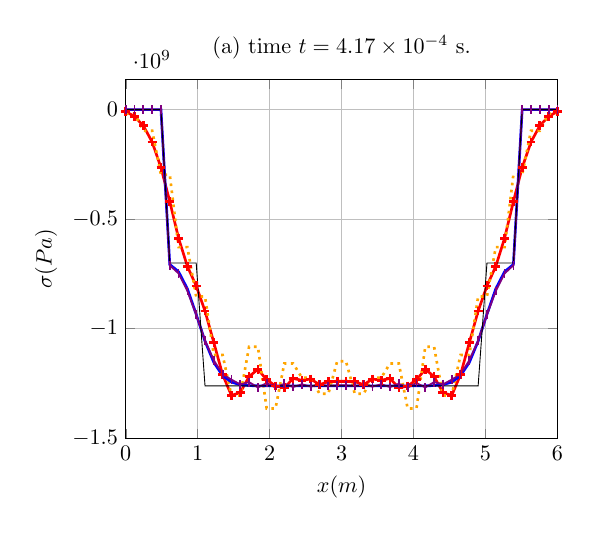
\begin{tikzpicture}[scale=0.8]
\begin{axis}[xlabel=$x (m)$,ylabel=$\sigma (Pa)$,ymajorgrids=true,xmajorgrids=true,legend pos=outer north east,title={(a) time $t = 4.17\times 10^{-4} $ s.},xmin=0.,xmax=6.]
\addplot[Red,very thick,mark=+,solid] coordinates {(0.0,-8433215.03790355) (0.12244897959183673,-31379937.150059074) (0.24489795918367346,-73325965.87671247) (0.36734693877551017,-147815909.35881704) (0.4897959183673469,-264501011.32373637) (0.6122448979591837,-419797360.6339785) (0.7346938775510203,-586994803.1537646) (0.8571428571428571,-715242874.2277462) (0.9795918367346939,-804731796.1198385) (1.1020408163265305,-919403784.9173691) (1.2244897959183674,-1063504114.033879) (1.346938775510204,-1209904754.949398) (1.4693877551020407,-1304654513.0867395) (1.5918367346938775,-1291382612.5749428) (1.7142857142857142,-1218226204.6353252) (1.836734693877551,-1185455835.0777807) (1.9591836734693877,-1232745182.470082) (2.0816326530612246,-1261396271.0817113) (2.204081632653061,-1270103667.4391637) (2.326530612244898,-1227250869.598082) (2.4489795918367347,-1235273389.504192) (2.571428571428571,-1229787858.686364) (2.693877551020408,-1255621316.42765) (2.816326530612245,-1241442333.7811728) (2.9387755102040813,-1239848703.7218106) (3.061224489795918,-1239848703.7218091) (3.183673469387755,-1241442333.781176) (3.306122448979592,-1255621316.4276485) (3.4285714285714284,-1229787858.6863654) (3.5510204081632653,-1235273389.5041904) (3.673469387755102,-1227250869.598084) (3.7959183673469385,-1270103667.439164) (3.9183673469387754,-1261396271.081712) (4.040816326530612,-1232745182.4700806) (4.163265306122449,-1185455835.0777805) (4.285714285714286,-1218226204.6353254) (4.408163265306122,-1291382612.5749435) (4.530612244897959,-1304654513.0867395) (4.653061224489796,-1209904754.9493968) (4.775510204081632,-1063504114.033878) (4.8979591836734695,-919403784.917369) (5.020408163265306,-804731796.1198374) (5.142857142857142,-715242874.2277458) (5.26530612244898,-586994803.1537648) (5.387755102040816,-419797360.63397753) (5.5102040816326525,-264501011.3237358) (5.63265306122449,-147815909.35881624) (5.755102040816326,-73325965.8767119) (5.877551020408163,-31379937.150058918) (6.0,-8433215.037903389) };
\addplot[Orange,very thick,mark=none,dotted] coordinates {(0.0,-19024028.854669835) (0.12244897959183673,-19024028.85467063) (0.24489795918367346,-96232491.2346082) (0.36734693877551017,-96232491.2346095) (0.4897959183673469,-297240710.94206506) (0.6122448979591837,-297240710.94206476) (0.7346938775510203,-627598280.4404582) (0.8571428571428571,-627598280.4404559) (0.9795918367346939,-853300561.8320081) (1.1020408163265305,-853300561.8320053) (1.2244897959183674,-1120326134.4042003) (1.346938775510204,-1120326134.4041946) (1.4693877551020407,-1305012184.0617018) (1.5918367346938775,-1305012184.061693) (1.7142857142857142,-1082408762.037375) (1.836734693877551,-1082408762.0373683) (1.9591836734693877,-1364071875.0838804) (2.0816326530612246,-1364071875.083866) (2.204081632653061,-1158492862.0093477) (2.326530612244898,-1158492862.0093355) (2.4489795918367347,-1223885693.6431794) (2.571428571428571,-1223885693.6431704) (2.693877551020408,-1296923820.0786731) (2.816326530612245,-1296923820.0786521) (2.9387755102040813,-1148570801.226303) (3.061224489795918,-1148570801.2262988) (3.183673469387755,-1296923820.0786695) (3.306122448979592,-1296923820.0786562) (3.4285714285714284,-1223885693.6431804) (3.5510204081632653,-1223885693.643168) (3.673469387755102,-1158492862.009347) (3.7959183673469385,-1158492862.0093367) (3.9183673469387754,-1364071875.083883) (4.040816326530612,-1364071875.0838625) (4.163265306122449,-1082408762.0373764) (4.285714285714286,-1082408762.0373673) (4.408163265306122,-1305012184.061705) (4.530612244897959,-1305012184.061689) (4.653061224489796,-1120326134.4042025) (4.775510204081632,-1120326134.4041922) (4.8979591836734695,-853300561.8320092) (5.020408163265306,-853300561.8320037) (5.142857142857142,-627598280.440458) (5.26530612244898,-627598280.440457) (5.387755102040816,-297240710.9420676) (5.5102040816326525,-297240710.9420631) (5.63265306122449,-96232491.23461069) (5.755102040816326,-96232491.23460749) (5.877551020408163,-19024028.85467079) (6.0,-19024028.85467007) };
\addplot[Blue,very thick,mark=none,solid] coordinates {(0.0,-3.2561158711216654e-07) (0.12244897959183673,-6.54162606232603e-22) (0.24489795918367346,0.0) (0.36734693877551017,3.2561158711216643e-07) (0.4897959183673469,-4.884173806682499e-07) (0.6122448979591837,-706703995.0062007) (0.7346938775510203,-739923853.3127105) (0.8571428571428571,-818114621.3278772) (0.9795918367346939,-934350667.0858994) (1.1020408163265305,-1056745717.4113452) (1.2244897959183674,-1153785079.176232) (1.346938775510204,-1213891661.9862223) (1.4693877551020407,-1243675875.166416) (1.5918367346938775,-1255667377.4619899) (1.7142857142857142,-1259628756.7765899) (1.836734693877551,-1260708382.472525) (1.9591836734693877,-1260951555.06527) (2.0816326530612246,-1260996741.6987677) (2.204081632653061,-1261003631.246593) (2.326530612244898,-1261004484.7294881) (2.4489795918367347,-1261004569.3136225) (2.571428571428571,-1261004575.8625927) (2.693877551020408,-1261004576.2443771) (2.816326530612245,-1261004576.2601426) (2.9387755102040813,-1261004576.2605536) (3.061224489795918,-1261004576.2605536) (3.183673469387755,-1261004576.2601426) (3.306122448979592,-1261004576.2443776) (3.4285714285714284,-1261004575.862593) (3.5510204081632653,-1261004569.3136227) (3.673469387755102,-1261004484.7294881) (3.7959183673469385,-1261003631.2465928) (3.9183673469387754,-1260996741.6987677) (4.040816326530612,-1260951555.0652697) (4.163265306122449,-1260708382.4725246) (4.285714285714286,-1259628756.7765894) (4.408163265306122,-1255667377.4619899) (4.530612244897959,-1243675875.1664157) (4.653061224489796,-1213891661.9862223) (4.775510204081632,-1153785079.176232) (4.8979591836734695,-1056745717.4113454) (5.020408163265306,-934350667.0858992) (5.142857142857142,-818114621.327877) (5.26530612244898,-739923853.3127109) (5.387755102040816,-706703995.0062011) (5.5102040816326525,-4.884173806682498e-07) (5.63265306122449,0.0) (5.755102040816326,-4.884173806682498e-07) (5.877551020408163,0.0) (6.0,-4.884173806682498e-07) };
\addplot[Purple,thick,mark=|,solid] coordinates {(0.0,-3.2561158711216654e-07) (0.12244897959183673,-6.54162606232603e-22) (0.24489795918367346,0.0) (0.36734693877551017,3.2561158711216643e-07) (0.4897959183673469,-4.884173806682499e-07) (0.6122448979591837,-710637837.2357953) (0.7346938775510203,-747893724.781927) (0.8571428571428571,-827829409.8631966) (0.9795918367346939,-936780409.853217) (1.1020408163265305,-1054073198.2499647) (1.2244897959183674,-1144128439.1849532) (1.346938775510204,-1207925723.6670742) (1.4693877551020407,-1232372577.7948787) (1.5918367346938775,-1254253728.274747) (1.7142857142857142,-1243570946.3490026) (1.836734693877551,-1268139963.2569304) (1.9591836734693877,-1248035262.8872383) (2.0816326530612246,-1268992337.693115) (2.204081632653061,-1251285653.8729925) (2.326530612244898,-1266352346.5241969) (2.4489795918367347,-1253527311.8706975) (2.571428571428571,-1264419055.233534) (2.693877551020408,-1255474245.0991223) (2.816326530612245,-1261578869.0693417) (2.9387755102040813,-1258168698.6750736) (3.061224489795918,-1258168698.6750731) (3.183673469387755,-1261578869.069342) (3.306122448979592,-1255474245.0991209) (3.4285714285714284,-1264419055.233534) (3.5510204081632653,-1253527311.870696) (3.673469387755102,-1266352346.5241973) (3.7959183673469385,-1251285653.8729923) (3.9183673469387754,-1268992337.6931143) (4.040816326530612,-1248035262.8872375) (4.163265306122449,-1268139963.2569308) (4.285714285714286,-1243570946.3490026) (4.408163265306122,-1254253728.2747467) (4.530612244897959,-1232372577.7948787) (4.653061224489796,-1207925723.6670735) (4.775510204081632,-1144128439.1849532) (4.8979591836734695,-1054073198.2499645) (5.020408163265306,-936780409.853217) (5.142857142857142,-827829409.8631967) (5.26530612244898,-747893724.7819276) (5.387755102040816,-710637837.2357956) (5.5102040816326525,-4.884173806682498e-07) (5.63265306122449,0.0) (5.755102040816326,-4.884173806682498e-07) (5.877551020408163,0.0) (6.0,-4.884173806682498e-07) };
\addplot[black,thin,mark=none,solid] coordinates {(0.0,-0.0) (0.12244897959183673,-0.0) (0.24489795918367346,-0.0) (0.36734693877551017,-0.0) (0.4897959183673469,-0.0) (0.6122448979591837,-700000000.0) (0.7346938775510203,-700000000.0) (0.8571428571428571,-700000000.0) (0.9795918367346939,-700000000.0) (1.1020408163265305,-1261004576.260559) (1.2244897959183674,-1261004576.260559) (1.346938775510204,-1261004576.260559) (1.4693877551020407,-1261004576.260559) (1.5918367346938775,-1261004576.260559) (1.7142857142857142,-1261004576.260559) (1.836734693877551,-1261004576.260559) (1.9591836734693877,-1261004576.260559) (2.0816326530612246,-1261004576.260559) (2.204081632653061,-1261004576.260559) (2.326530612244898,-1261004576.260559) (2.4489795918367347,-1261004576.260559) (2.571428571428571,-1261004576.260559) (2.693877551020408,-1261004576.260559) (2.816326530612245,-1261004576.260559) (2.9387755102040813,-1261004576.260559) (3.061224489795918,-1261004576.260559) (3.183673469387755,-1261004576.260559) (3.306122448979592,-1261004576.260559) (3.4285714285714284,-1261004576.260559) (3.5510204081632653,-1261004576.260559) (3.673469387755102,-1261004576.260559) (3.7959183673469385,-1261004576.260559) (3.9183673469387754,-1261004576.260559) (4.040816326530612,-1261004576.260559) (4.163265306122449,-1261004576.260559) (4.285714285714286,-1261004576.260559) (4.408163265306122,-1261004576.260559) (4.530612244897959,-1261004576.260559) (4.653061224489796,-1261004576.260559) (4.775510204081632,-1261004576.260559) (4.8979591836734695,-1261004576.260559) (5.020408163265306,-700000000.0) (5.142857142857142,-700000000.0) (5.26530612244898,-700000000.0) (5.387755102040816,-700000000.0) (5.5102040816326525,-0.0) (5.63265306122449,-0.0) (5.755102040816326,-0.0) (5.877551020408163,-0.0) (6.0,-0.0) };
%\legend{usl,usf,dgmpm (ep solver),dgmpm (ac solver),exact}
\end{axis}
\end{tikzpicture}
%%% Local Variables:
%%% mode: latex
%%% TeX-master: "../../mainManuscript"
%%% End:
}
  % {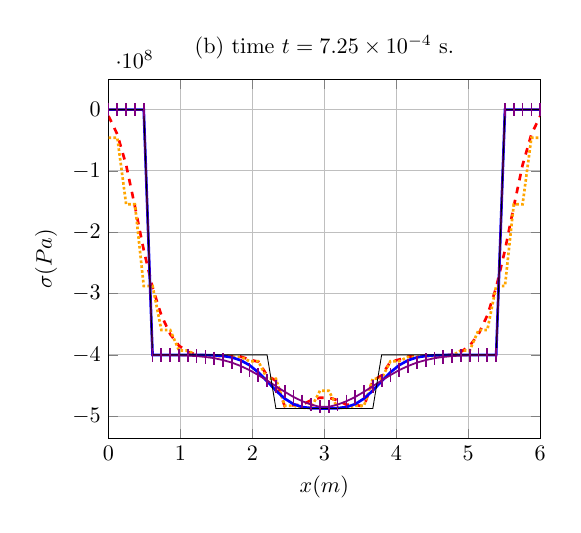
\begin{tikzpicture}[scale=0.8]
\begin{axis}[xlabel=$x (m)$,ylabel=$\sigma (Pa)$,ymajorgrids=true,xmajorgrids=true,legend pos=outer north east,title={(b) time $t = 7.25\times 10^{-4} $ s.},xmin=0.,xmax=6.]
\addplot[Red,very thick,mark=none,dashed,mark size=3pt] coordinates {(0.0,-10477027.22040739) (0.12244897959183673,-40202439.77672757) (0.24489795918367346,-90268409.98400429) (0.36734693877551017,-157917330.96394995) (0.4897959183673469,-229098117.24026006) (0.6122448979591837,-290170966.79273176) (0.7346938775510203,-335449952.79523534) (0.8571428571428571,-366063963.8356788) (0.9795918367346939,-384934670.81956863) (1.1020408163265305,-394978768.22705775) (1.2244897959183674,-399539747.49342227) (1.346938775510204,-401064801.98949975) (1.4693877551020407,-401261686.3649931) (1.5918367346938775,-401362011.1717392) (1.7142857142857142,-402125702.7814173) (1.836734693877551,-402648608.50963366) (1.9591836734693877,-407517028.59914577) (2.0816326530612246,-411133976.99807984) (2.204081632653061,-433339939.374477) (2.326530612244898,-442099776.2163934) (2.4489795918367347,-483576545.68129754) (2.571428571428571,-481854124.4484605) (2.693877551020408,-481095256.73223835) (2.816326530612245,-473792554.1947772) (2.9387755102040813,-469732138.6842222) (3.061224489795918,-469732138.6842212) (3.183673469387755,-473792554.1947779) (3.306122448979592,-481095256.73223734) (3.4285714285714284,-481854124.4484616) (3.5510204081632653,-483576545.6812961) (3.673469387755102,-442099776.2163934) (3.7959183673469385,-433339939.3744765) (3.9183673469387754,-411133976.99807984) (4.040816326530612,-407517028.5991456) (4.163265306122449,-402648608.50963354) (4.285714285714286,-402125702.78141725) (4.408163265306122,-401362011.1717393) (4.530612244897959,-401261686.3649931) (4.653061224489796,-401064801.9894998) (4.775510204081632,-399539747.4934223) (4.8979591836734695,-394978768.22705775) (5.020408163265306,-384934670.81956846) (5.142857142857142,-366063963.83567846) (5.26530612244898,-335449952.79523504) (5.387755102040816,-290170966.7927308) (5.5102040816326525,-229098117.24025902) (5.63265306122449,-157917330.96394882) (5.755102040816326,-90268409.98400334) (5.877551020408163,-40202439.77672676) (6.0,-10477027.22040709) };
\addplot[Orange,very thick,mark=none,densely dotted,mark size=3pt] coordinates {(0.0,-45848801.116061755) (0.12244897959183673,-45848801.11606384) (0.24489795918367346,-154376178.19250378) (0.36734693877551017,-154376178.19250578) (0.4897959183673469,-287527291.433164) (0.6122448979591837,-287527291.4331672) (0.7346938775510203,-359292004.22399014) (0.8571428571428571,-359292004.2239917) (0.9795918367346939,-392683727.4502954) (1.1020408163265305,-392683727.4502976) (1.2244897959183674,-401164708.0318632) (1.346938775510204,-401164708.03186363) (1.4693877551020407,-401759751.30394024) (1.5918367346938775,-401759751.30394024) (1.7142857142857142,-403128689.3401794) (1.836734693877551,-403128689.34017944) (1.9591836734693877,-410178577.79555696) (2.0816326530612246,-410178577.79555744) (2.204081632653061,-438610352.6160444) (2.326530612244898,-438610352.61604387) (2.4489795918367347,-482851170.1855085) (2.571428571428571,-482851170.1855071) (2.693877551020408,-486171580.9073176) (2.816326530612245,-486171580.9073155) (2.9387755102040813,-458406821.6261096) (3.061224489795918,-458406821.6261075) (3.183673469387755,-486171580.90731794) (3.306122448979592,-486171580.90731514) (3.4285714285714284,-482851170.18550956) (3.5510204081632653,-482851170.1855064) (3.673469387755102,-438610352.61604464) (3.7959183673469385,-438610352.6160435) (3.9183673469387754,-410178577.7955573) (4.040816326530612,-410178577.79555714) (4.163265306122449,-403128689.3401792) (4.285714285714286,-403128689.34017956) (4.408163265306122,-401759751.3039401) (4.530612244897959,-401759751.30394024) (4.653061224489796,-401164708.0318638) (4.775510204081632,-401164708.0318631) (4.8979591836734695,-392683727.4502974) (5.020408163265306,-392683727.4502955) (5.142857142857142,-359292004.22399014) (5.26530612244898,-359292004.2239912) (5.387755102040816,-287527291.4331645) (5.5102040816326525,-287527291.4331666) (5.63265306122449,-154376178.19250128) (5.755102040816326,-154376178.1925081) (5.877551020408163,-45848801.11605563) (6.0,-45848801.11606924) };
\addplot[Blue,very thick,mark=none,solid,mark size=3pt] coordinates {(0.0,-0.016398596440346053) (0.12244897959183673,-0.06425322857955201) (0.24489795918367346,-0.7380674881804443) (0.36734693877551017,-2.12047390173559) (0.4897959183673469,-28.76271861558054) (0.6122448979591837,-400000015.4159754) (0.7346938775510203,-400000102.7573024) (0.8571428571428571,-400000598.1932516) (0.9795918367346939,-400003055.79803795) (1.1020408163265305,-400013747.0436081) (1.2244897959183674,-400054602.7199052) (1.346938775510204,-400191823.2382515) (1.4693877551020407,-400596672.6802674) (1.5918367346938775,-401644186.51493835) (1.7142857142857142,-404014374.4754996) (1.836734693877551,-408684632.25449073) (1.9591836734693877,-416652037.9726774) (2.0816326530612246,-428329061.0045163) (2.204081632653061,-442879954.5361007) (2.326530612244898,-458084443.80872595) (2.4489795918367347,-471157539.9020842) (2.571428571428571,-480164339.19475454) (2.693877551020408,-484944715.5259052) (2.816326530612245,-486779650.5319825) (2.9387755102040813,-487233015.60471344) (3.061224489795918,-487233015.60471344) (3.183673469387755,-486779650.5319825) (3.306122448979592,-484944715.5259052) (3.4285714285714284,-480164339.19475454) (3.5510204081632653,-471157539.9020842) (3.673469387755102,-458084443.80872613) (3.7959183673469385,-442879954.5361007) (3.9183673469387754,-428329061.0045163) (4.040816326530612,-416652037.9726776) (4.163265306122449,-408684632.2544908) (4.285714285714286,-404014374.4754996) (4.408163265306122,-401644186.5149382) (4.530612244897959,-400596672.68026733) (4.653061224489796,-400191823.2382513) (4.775510204081632,-400054602.7199051) (4.8979591836734695,-400013747.04360807) (5.020408163265306,-400003055.79803795) (5.142857142857142,-400000598.19325155) (5.26530612244898,-400000102.75730234) (5.387755102040816,-400000015.4159754) (5.5102040816326525,-28.762718512303003) (5.63265306122449,-2.1204742438100417) (5.755102040816326,-0.7380675867576459) (5.877551020408163,-0.06425320166977637) (6.0,-0.01639854380134023) };
\addplot[Purple,thick,mark=|,solid,mark size=3pt] coordinates {(0.0,-6603.656961914038) (0.12244897959183673,-24301.815008368238) (0.24489795918367346,-55464.41985537122) (0.36734693877551017,-106156.2537208052) (0.4897959183673469,-211897.6201172594) (0.6122448979591837,-400060577.70226735) (0.7346938775510203,-400131812.16225874) (0.8571428571428571,-400283732.27719015) (0.9795918367346939,-400555327.2203242) (1.1020408163265305,-401066737.28576595) (1.2244897959183674,-401894072.0480914) (1.346938775510204,-403284345.7790878) (1.4693877551020407,-405323949.9831428) (1.5918367346938775,-408400739.0278849) (1.7142857142857142,-412492331.79054075) (1.836734693877551,-418043336.8286237) (1.9591836734693877,-424711534.45864564) (2.0816326530612246,-432827603.874204) (2.204081632653061,-441566942.10959697) (2.326530612244898,-451030928.52523047) (2.4489795918367347,-460033248.5355418) (2.571428571428571,-468546974.69264907) (2.693877551020408,-475502563.6678834) (2.816326530612245,-481002410.6287537) (2.9387755102040813,-484629369.3636542) (3.061224489795918,-484629369.3636542) (3.183673469387755,-481002410.6287537) (3.306122448979592,-475502563.6678834) (3.4285714285714284,-468546974.69264907) (3.5510204081632653,-460033248.5355418) (3.673469387755102,-451030928.52523047) (3.7959183673469385,-441566942.10959697) (3.9183673469387754,-432827603.874204) (4.040816326530612,-424711534.4586456) (4.163265306122449,-418043336.82862353) (4.285714285714286,-412492331.79054075) (4.408163265306122,-408400739.0278848) (4.530612244897959,-405323949.9831428) (4.653061224489796,-403284345.7790876) (4.775510204081632,-401894072.0480913) (4.8979591836734695,-401066737.28576595) (5.020408163265306,-400555327.2203241) (5.142857142857142,-400283732.2771901) (5.26530612244898,-400131812.16225874) (5.387755102040816,-400060577.70226735) (5.5102040816326525,-211897.6201168723) (5.63265306122449,-106156.25372073636) (5.755102040816326,-55464.41985543468) (5.877551020408163,-24301.815008351048) (6.0,-6603.6569619941265) };
\addplot[black,thin,mark=none,solid,mark size=3pt] coordinates {(0.0,-0.0) (0.12244897959183673,-0.0) (0.24489795918367346,-0.0) (0.36734693877551017,-0.0) (0.4897959183673469,-0.0) (0.6122448979591837,-400000000.0) (0.7346938775510203,-400000000.0) (0.8571428571428571,-400000000.0) (0.9795918367346939,-400000000.0) (1.1020408163265305,-400000000.0) (1.2244897959183674,-400000000.0) (1.346938775510204,-400000000.0) (1.4693877551020407,-400000000.0) (1.5918367346938775,-400000000.0) (1.7142857142857142,-400000000.0) (1.836734693877551,-400000000.0) (1.9591836734693877,-400000000.0) (2.0816326530612246,-400000000.0) (2.204081632653061,-400000000.0) (2.326530612244898,-487287156.09439695) (2.4489795918367347,-487287156.09439695) (2.571428571428571,-487287156.09439695) (2.693877551020408,-487287156.09439695) (2.816326530612245,-487287156.09439695) (2.9387755102040813,-487287156.09439695) (3.061224489795918,-487287156.09439695) (3.183673469387755,-487287156.09439695) (3.306122448979592,-487287156.09439695) (3.4285714285714284,-487287156.09439695) (3.5510204081632653,-487287156.09439695) (3.673469387755102,-487287156.09439695) (3.7959183673469385,-400000000.0) (3.9183673469387754,-400000000.0) (4.040816326530612,-400000000.0) (4.163265306122449,-400000000.0) (4.285714285714286,-400000000.0) (4.408163265306122,-400000000.0) (4.530612244897959,-400000000.0) (4.653061224489796,-400000000.0) (4.775510204081632,-400000000.0) (4.8979591836734695,-400000000.0) (5.020408163265306,-400000000.0) (5.142857142857142,-400000000.0) (5.26530612244898,-400000000.0) (5.387755102040816,-400000000.0) (5.5102040816326525,-0.0) (5.63265306122449,-0.0) (5.755102040816326,-0.0) (5.877551020408163,-0.0) (6.0,-0.0) };
%\legend{usl,usf,dgmpm (ep solver),dgmpm (ac solver),exact}
\end{axis}
\end{tikzpicture}
%%% Local Variables:
%%% mode: latex
%%% TeX-master: "../../mainManuscript"
%%% End:
}
  {% \begin{tikzpicture}[scale=0.4]
% \begin{groupplot}[group style={group size=1 by 1,
% ylabels at=edge left, yticklabels at=edge left,horizontal sep=2.ex,
% vertical sep=4ex,xticklabels at=edge bottom,xlabels at=edge bottom},
% ymajorgrids=true,xmajorgrids=true,enlargelimits=0,xmin=0.,xmax=6.,xlabel=$x (m)$,
% axis on top,scale only axis
% ]
% % \nextgroupplot[ylabel=$\sigma (Pa)$,title={$t = 4.17\times 10^{-4} $ s.},ymin=-1.35e9,ymax=56579516.10614197,]
% % \addplot[Blue,solid,mark=x,very thick,mark size=3pt,mark repeat=3] coordinates{(0.0,-3.2561158711216654e-07) (0.12244897959183673,-6.54162606232603e-22) (0.24489795918367346,0.0) (0.36734693877551017,3.2561158711216643e-07) (0.4897959183673469,-4.884173806682499e-07) (0.6122448979591837,-706703995.0062007) (0.7346938775510203,-739923853.3127105) (0.8571428571428571,-818114621.3278772) (0.9795918367346939,-934350667.0858994) (1.1020408163265305,-1056745717.4113452) (1.2244897959183674,-1153785079.176232) (1.346938775510204,-1213891661.9862223) (1.4693877551020407,-1243675875.166416) (1.5918367346938775,-1255667377.4619899) (1.7142857142857142,-1259628756.7765899) (1.836734693877551,-1260708382.472525) (1.9591836734693877,-1260951555.06527) (2.0816326530612246,-1260996741.6987677) (2.204081632653061,-1261003631.246593) (2.326530612244898,-1261004484.7294881) (2.4489795918367347,-1261004569.3136225) (2.571428571428571,-1261004575.8625927) (2.693877551020408,-1261004576.2443771) (2.816326530612245,-1261004576.2601426) (2.9387755102040813,-1261004576.2605536) (3.061224489795918,-1261004576.2605536) (3.183673469387755,-1261004576.2601426) (3.306122448979592,-1261004576.2443776) (3.4285714285714284,-1261004575.862593) (3.5510204081632653,-1261004569.3136227) (3.673469387755102,-1261004484.7294881) (3.7959183673469385,-1261003631.2465928) (3.9183673469387754,-1260996741.6987677) (4.040816326530612,-1260951555.0652697) (4.163265306122449,-1260708382.4725246) (4.285714285714286,-1259628756.7765894) (4.408163265306122,-1255667377.4619899) (4.530612244897959,-1243675875.1664157) (4.653061224489796,-1213891661.9862223) (4.775510204081632,-1153785079.176232) (4.8979591836734695,-1056745717.4113454) (5.020408163265306,-934350667.0858992) (5.142857142857142,-818114621.327877) (5.26530612244898,-739923853.3127109) (5.387755102040816,-706703995.0062011) (5.5102040816326525,-4.884173806682498e-07) (5.63265306122449,0.0) (5.755102040816326,-4.884173806682498e-07) (5.877551020408163,0.0) (6.0,-4.884173806682498e-07) };
% % \addplot[Purple,solid,mark=+,thick,mark size=3pt,mark repeat=3] coordinates{(0.0,-3.2561158711216654e-07) (0.12244897959183673,-6.54162606232603e-22) (0.24489795918367346,0.0) (0.36734693877551017,3.2561158711216643e-07) (0.4897959183673469,-4.884173806682499e-07) (0.6122448979591837,-710637837.2357953) (0.7346938775510203,-747893724.781927) (0.8571428571428571,-827829409.8631966) (0.9795918367346939,-936780409.853217) (1.1020408163265305,-1054073198.2499647) (1.2244897959183674,-1144128439.1849532) (1.346938775510204,-1207925723.6670742) (1.4693877551020407,-1232372577.7948787) (1.5918367346938775,-1254253728.274747) (1.7142857142857142,-1243570946.3490026) (1.836734693877551,-1268139963.2569304) (1.9591836734693877,-1248035262.8872383) (2.0816326530612246,-1268992337.693115) (2.204081632653061,-1251285653.8729925) (2.326530612244898,-1266352346.5241969) (2.4489795918367347,-1253527311.8706975) (2.571428571428571,-1264419055.233534) (2.693877551020408,-1255474245.0991223) (2.816326530612245,-1261578869.0693417) (2.9387755102040813,-1258168698.6750736) (3.061224489795918,-1258168698.6750731) (3.183673469387755,-1261578869.069342) (3.306122448979592,-1255474245.0991209) (3.4285714285714284,-1264419055.233534) (3.5510204081632653,-1253527311.870696) (3.673469387755102,-1266352346.5241973) (3.7959183673469385,-1251285653.8729923) (3.9183673469387754,-1268992337.6931143) (4.040816326530612,-1248035262.8872375) (4.163265306122449,-1268139963.2569308) (4.285714285714286,-1243570946.3490026) (4.408163265306122,-1254253728.2747467) (4.530612244897959,-1232372577.7948787) (4.653061224489796,-1207925723.6670735) (4.775510204081632,-1144128439.1849532) (4.8979591836734695,-1054073198.2499645) (5.020408163265306,-936780409.853217) (5.142857142857142,-827829409.8631967) (5.26530612244898,-747893724.7819276) (5.387755102040816,-710637837.2357956) (5.5102040816326525,-4.884173806682498e-07) (5.63265306122449,0.0) (5.755102040816326,-4.884173806682498e-07) (5.877551020408163,0.0) (6.0,-4.884173806682498e-07) };
% % \addplot[black,solid,mark=none,thin,mark size=3pt,mark repeat=3] coordinates{(0.0,-0.0) (0.12244897959183673,-0.0) (0.24489795918367346,-0.0) (0.36734693877551017,-0.0) (0.4897959183673469,-0.0) (0.6122448979591837,-700000000.0) (0.7346938775510203,-700000000.0) (0.8571428571428571,-700000000.0) (0.9795918367346939,-700000000.0) (1.1020408163265305,-1261004576.260559) (1.2244897959183674,-1261004576.260559) (1.346938775510204,-1261004576.260559) (1.4693877551020407,-1261004576.260559) (1.5918367346938775,-1261004576.260559) (1.7142857142857142,-1261004576.260559) (1.836734693877551,-1261004576.260559) (1.9591836734693877,-1261004576.260559) (2.0816326530612246,-1261004576.260559) (2.204081632653061,-1261004576.260559) (2.326530612244898,-1261004576.260559) (2.4489795918367347,-1261004576.260559) (2.571428571428571,-1261004576.260559) (2.693877551020408,-1261004576.260559) (2.816326530612245,-1261004576.260559) (2.9387755102040813,-1261004576.260559) (3.061224489795918,-1261004576.260559) (3.183673469387755,-1261004576.260559) (3.306122448979592,-1261004576.260559) (3.4285714285714284,-1261004576.260559) (3.5510204081632653,-1261004576.260559) (3.673469387755102,-1261004576.260559) (3.7959183673469385,-1261004576.260559) (3.9183673469387754,-1261004576.260559) (4.040816326530612,-1261004576.260559) (4.163265306122449,-1261004576.260559) (4.285714285714286,-1261004576.260559) (4.408163265306122,-1261004576.260559) (4.530612244897959,-1261004576.260559) (4.653061224489796,-1261004576.260559) (4.775510204081632,-1261004576.260559) (4.8979591836734695,-1261004576.260559) (5.020408163265306,-700000000.0) (5.142857142857142,-700000000.0) (5.26530612244898,-700000000.0) (5.387755102040816,-700000000.0) (5.5102040816326525,-0.0) (5.63265306122449,-0.0) (5.755102040816326,-0.0) (5.877551020408163,-0.0) (6.0,-0.0) };
% \nextgroupplot[ylabel=$\eps^p $,ymin=-0.0021,ymax=0.0,title={Elastic-plastic plane waves}]
% \addplot[Blue,solid,mark=x,very thick,mark size=3pt,mark repeat=3] coordinates{(0.0,0.0) (0.12244897959183673,0.0) (0.24489795918367346,0.0) (0.36734693877551017,0.0) (0.4897959183673469,0.0) (0.6122448979591837,-2.4267855226065594e-05) (0.7346938775510203,-0.00014452073597361284) (0.8571428571428571,-0.0004275642401009131) (0.9795918367346939,-0.0008483282066457896) (1.1020408163265305,-0.0012913872123487611) (1.2244897959183674,-0.001642660920094959) (1.346938775510204,-0.0018602413103573651) (1.4693877551020407,-0.0019680574666657586) (1.5918367346938775,-0.00201146561977191) (1.7142857142857142,-0.002025805454394895) (1.836734693877551,-0.0020297136017104972) (1.9591836734693877,-0.002030593864489664) (2.0816326530612246,-0.002030757436013639) (2.204081632653061,-0.0020307823755532774) (2.326530612244898,-0.002030785465084119) (2.4489795918367347,-0.0020307857712710334) (2.571428571428571,-0.00203078579497771) (2.693877551020408,-0.0020307857963597366) (2.816326530612245,-0.002030785796416807) (2.9387755102040813,-0.002030785796418294) (3.061224489795918,-0.002030785796418294) (3.183673469387755,-0.0020307857964168056) (3.306122448979592,-0.002030785796359739) (3.4285714285714284,-0.0020307857949777124) (3.5510204081632653,-0.002030785771271032) (3.673469387755102,-0.002030785465084119) (3.7959183673469385,-0.002030782375553277) (3.9183673469387754,-0.0020307574360136386) (4.040816326530612,-0.002030593864489664) (4.163265306122449,-0.0020297136017104964) (4.285714285714286,-0.0020258054543948927) (4.408163265306122,-0.002011465619771909) (4.530612244897959,-0.0019680574666657573) (4.653061224489796,-0.0018602413103573651) (4.775510204081632,-0.0016426609200949592) (4.8979591836734695,-0.001291387212348762) (5.020408163265306,-0.0008483282066457893) (5.142857142857142,-0.00042756424010091193) (5.26530612244898,-0.00014452073597361384) (5.387755102040816,-2.4267855226067292e-05) (5.5102040816326525,0.0) (5.63265306122449,0.0) (5.755102040816326,0.0) (5.877551020408163,0.0) (6.0,0.0) };
% \addplot[Purple,solid,mark=+,thick,mark size=3pt,mark repeat=3] coordinates{(0.0,0.0) (0.12244897959183673,0.0) (0.24489795918367346,0.0) (0.36734693877551017,0.0) (0.4897959183673469,0.0) (0.6122448979591837,-3.850800809337606e-05) (0.7346938775510203,-0.00017337094943683953) (0.8571428571428571,-0.00046273089543238553) (0.9795918367346939,-0.000857123655577256) (1.1020408163265305,-0.0012817129348415013) (1.2244897959183674,-0.0016077047572306) (1.346938775510204,-0.0018386451535459692) (1.4693877551020407,-0.0019271405531036338) (1.5918367346938775,-0.002006348337646142) (1.7142857142857142,-0.002018045326373221) (1.836734693877551,-0.002056615251608797) (1.9591836734693877,-0.0020613216365693464) (2.0816326530612246,-0.002064203896841495) (2.204081632653061,-0.0020644266901542695) (2.326530612244898,-0.0020621094945296272) (2.4489795918367347,-0.002062767607181189) (2.571428571428571,-0.002061489252343496) (2.693877551020408,-0.0020573197208032658) (2.816326530612245,-0.0020502799029179) (2.9387755102040813,-0.0020377776694292327) (3.061224489795918,-0.0020377776694292327) (3.183673469387755,-0.002050279902917899) (3.306122448979592,-0.002057319720803265) (3.4285714285714284,-0.0020614892523434956) (3.5510204081632653,-0.0020627676071811878) (3.673469387755102,-0.0020621094945296285) (3.7959183673469385,-0.0020644266901542695) (3.9183673469387754,-0.0020642038968414953) (4.040816326530612,-0.0020613216365693477) (4.163265306122449,-0.002056615251608799) (4.285714285714286,-0.0020180453263732205) (4.408163265306122,-0.0020063483376461405) (4.530612244897959,-0.0019271405531036334) (4.653061224489796,-0.0018386451535459673) (4.775510204081632,-0.0016077047572305996) (4.8979591836734695,-0.0012817129348415002) (5.020408163265306,-0.0008571236555772557) (5.142857142857142,-0.000462730895432386) (5.26530612244898,-0.0001733709494368422) (5.387755102040816,-3.850800809337776e-05) (5.5102040816326525,0.0) (5.63265306122449,0.0) (5.755102040816326,0.0) (5.877551020408163,0.0) (6.0,0.0) };
% \addplot[black,solid,mark=none,thin,mark size=3pt,mark repeat=3] coordinates{(0.0,-0.0) (0.12244897959183673,-0.0) (0.24489795918367346,-0.0) (0.36734693877551017,-0.0) (0.4897959183673469,-0.0) (0.6122448979591837,-0.0) (0.7346938775510203,-0.0) (0.8571428571428571,-0.0) (0.9795918367346939,-0.0) (1.1020408163265305,-0.002030785796418313) (1.2244897959183674,-0.002030785796418313) (1.346938775510204,-0.002030785796418313) (1.4693877551020407,-0.002030785796418313) (1.5918367346938775,-0.002030785796418313) (1.7142857142857142,-0.002030785796418313) (1.836734693877551,-0.002030785796418313) (1.9591836734693877,-0.002030785796418313) (2.0816326530612246,-0.002030785796418313) (2.204081632653061,-0.002030785796418313) (2.326530612244898,-0.002030785796418313) (2.4489795918367347,-0.002030785796418313) (2.571428571428571,-0.002030785796418313) (2.693877551020408,-0.002030785796418313) (2.816326530612245,-0.002030785796418313) (2.9387755102040813,-0.002030785796418313) (3.061224489795918,-0.002030785796418313) (3.183673469387755,-0.002030785796418313) (3.306122448979592,-0.002030785796418313) (3.4285714285714284,-0.002030785796418313) (3.5510204081632653,-0.002030785796418313) (3.673469387755102,-0.002030785796418313) (3.7959183673469385,-0.002030785796418313) (3.9183673469387754,-0.002030785796418313) (4.040816326530612,-0.002030785796418313) (4.163265306122449,-0.002030785796418313) (4.285714285714286,-0.002030785796418313) (4.408163265306122,-0.002030785796418313) (4.530612244897959,-0.002030785796418313) (4.653061224489796,-0.002030785796418313) (4.775510204081632,-0.002030785796418313) (4.8979591836734695,-0.002030785796418313) (5.020408163265306,-0.0) (5.142857142857142,-0.0) (5.26530612244898,-0.0) (5.387755102040816,-0.0) (5.5102040816326525,-0.0) (5.63265306122449,-0.0) (5.755102040816326,-0.0) (5.877551020408163,-0.0) (6.0,-0.0) };

% \addlegendentry{fvm (elastic-plastic Riemann solver)}
% \addlegendentry{fvm (elastic Riemann solver)}
% \addlegendentry{exact}

% \end{groupplot}
% \end{tikzpicture}


\begin{tikzpicture}[spy using outlines={rectangle, magnification=2, size=.15cm, connect spies},scale=0.7]
\begin{axis}[xlabel=$x \:(\text{m})$,ylabel=$\eps^p $,ymajorgrids=true,xmajorgrids=true,legend pos=north east,title={Plastic waves},xmin=0.,xmax=6.,ymin=-0.0021,ymax=0.00001]
\addplot[Blue,solid,mark=x,very thick,mark size=3pt,mark repeat=3] coordinates{(0.0,0.0) (0.12244897959183673,0.0) (0.24489795918367346,0.0) (0.36734693877551017,0.0) (0.4897959183673469,0.0) (0.6122448979591837,-2.4267855226065594e-05) (0.7346938775510203,-0.00014452073597361284) (0.8571428571428571,-0.0004275642401009131) (0.9795918367346939,-0.0008483282066457896) (1.1020408163265305,-0.0012913872123487611) (1.2244897959183674,-0.001642660920094959) (1.346938775510204,-0.0018602413103573651) (1.4693877551020407,-0.0019680574666657586) (1.5918367346938775,-0.00201146561977191) (1.7142857142857142,-0.002025805454394895) (1.836734693877551,-0.0020297136017104972) (1.9591836734693877,-0.002030593864489664) (2.0816326530612246,-0.002030757436013639) (2.204081632653061,-0.0020307823755532774) (2.326530612244898,-0.002030785465084119) (2.4489795918367347,-0.0020307857712710334) (2.571428571428571,-0.00203078579497771) (2.693877551020408,-0.0020307857963597366) (2.816326530612245,-0.002030785796416807) (2.9387755102040813,-0.002030785796418294) (3.061224489795918,-0.002030785796418294) (3.183673469387755,-0.0020307857964168056) (3.306122448979592,-0.002030785796359739) (3.4285714285714284,-0.0020307857949777124) (3.5510204081632653,-0.002030785771271032) (3.673469387755102,-0.002030785465084119) (3.7959183673469385,-0.002030782375553277) (3.9183673469387754,-0.0020307574360136386) (4.040816326530612,-0.002030593864489664) (4.163265306122449,-0.0020297136017104964) (4.285714285714286,-0.0020258054543948927) (4.408163265306122,-0.002011465619771909) (4.530612244897959,-0.0019680574666657573) (4.653061224489796,-0.0018602413103573651) (4.775510204081632,-0.0016426609200949592) (4.8979591836734695,-0.001291387212348762) (5.020408163265306,-0.0008483282066457893) (5.142857142857142,-0.00042756424010091193) (5.26530612244898,-0.00014452073597361384) (5.387755102040816,-2.4267855226067292e-05) (5.5102040816326525,0.0) (5.63265306122449,0.0) (5.755102040816326,0.0) (5.877551020408163,0.0) (6.0,0.0) };
\addplot[Red,solid,mark=+,very thick,mark size=3pt,mark repeat=3] coordinates{(0.0,0.0) (0.12244897959183673,0.0) (0.24489795918367346,0.0) (0.36734693877551017,0.0) (0.4897959183673469,0.0) (0.6122448979591837,-3.850800809337606e-05) (0.7346938775510203,-0.00017337094943683953) (0.8571428571428571,-0.00046273089543238553) (0.9795918367346939,-0.000857123655577256) (1.1020408163265305,-0.0012817129348415013) (1.2244897959183674,-0.0016077047572306) (1.346938775510204,-0.0018386451535459692) (1.4693877551020407,-0.0019271405531036338) (1.5918367346938775,-0.002006348337646142) (1.7142857142857142,-0.002018045326373221) (1.836734693877551,-0.002056615251608797) (1.9591836734693877,-0.0020613216365693464) (2.0816326530612246,-0.002064203896841495) (2.204081632653061,-0.0020644266901542695) (2.326530612244898,-0.0020621094945296272) (2.4489795918367347,-0.002062767607181189) (2.571428571428571,-0.002061489252343496) (2.693877551020408,-0.0020573197208032658) (2.816326530612245,-0.0020502799029179) (2.9387755102040813,-0.0020377776694292327) (3.061224489795918,-0.0020377776694292327) (3.183673469387755,-0.002050279902917899) (3.306122448979592,-0.002057319720803265) (3.4285714285714284,-0.0020614892523434956) (3.5510204081632653,-0.0020627676071811878) (3.673469387755102,-0.0020621094945296285) (3.7959183673469385,-0.0020644266901542695) (3.9183673469387754,-0.0020642038968414953) (4.040816326530612,-0.0020613216365693477) (4.163265306122449,-0.002056615251608799) (4.285714285714286,-0.0020180453263732205) (4.408163265306122,-0.0020063483376461405) (4.530612244897959,-0.0019271405531036334) (4.653061224489796,-0.0018386451535459673) (4.775510204081632,-0.0016077047572305996) (4.8979591836734695,-0.0012817129348415002) (5.020408163265306,-0.0008571236555772557) (5.142857142857142,-0.000462730895432386) (5.26530612244898,-0.0001733709494368422) (5.387755102040816,-3.850800809337776e-05) (5.5102040816326525,0.0) (5.63265306122449,0.0) (5.755102040816326,0.0) (5.877551020408163,0.0) (6.0,0.0) };
\addplot[black,solid,mark=none,thick,mark size=3pt,mark repeat=3] coordinates{(0.0,-0.0) (0.12244897959183673,-0.0) (0.24489795918367346,-0.0) (0.36734693877551017,-0.0) (0.4897959183673469,-0.0) (0.6122448979591837,-0.0) (0.7346938775510203,-0.0) (0.8571428571428571,-0.0) (0.9795918367346939,-0.0) (1.1020408163265305,-0.002030785796418313) (1.2244897959183674,-0.002030785796418313) (1.346938775510204,-0.002030785796418313) (1.4693877551020407,-0.002030785796418313) (1.5918367346938775,-0.002030785796418313) (1.7142857142857142,-0.002030785796418313) (1.836734693877551,-0.002030785796418313) (1.9591836734693877,-0.002030785796418313) (2.0816326530612246,-0.002030785796418313) (2.204081632653061,-0.002030785796418313) (2.326530612244898,-0.002030785796418313) (2.4489795918367347,-0.002030785796418313) (2.571428571428571,-0.002030785796418313) (2.693877551020408,-0.002030785796418313) (2.816326530612245,-0.002030785796418313) (2.9387755102040813,-0.002030785796418313) (3.061224489795918,-0.002030785796418313) (3.183673469387755,-0.002030785796418313) (3.306122448979592,-0.002030785796418313) (3.4285714285714284,-0.002030785796418313) (3.5510204081632653,-0.002030785796418313) (3.673469387755102,-0.002030785796418313) (3.7959183673469385,-0.002030785796418313) (3.9183673469387754,-0.002030785796418313) (4.040816326530612,-0.002030785796418313) (4.163265306122449,-0.002030785796418313) (4.285714285714286,-0.002030785796418313) (4.408163265306122,-0.002030785796418313) (4.530612244897959,-0.002030785796418313) (4.653061224489796,-0.002030785796418313) (4.775510204081632,-0.002030785796418313) (4.8979591836734695,-0.002030785796418313) (5.020408163265306,-0.0) (5.142857142857142,-0.0) (5.26530612244898,-0.0) (5.387755102040816,-0.0) (5.5102040816326525,-0.0) (5.63265306122449,-0.0) (5.755102040816326,-0.0) (5.877551020408163,-0.0) (6.0,-0.0) };
\begin{scope}
\spy[black,size=1.5cm] on (1.45,0.3) in node [fill=none] at (3.5,2.7);
\end{scope}

\legend{fvm ("elastic-plastic" fluxes),fvm ("elastic" fluxes),exact}
\end{axis}
\end{tikzpicture}
%%% Local Variables:
%%% mode: latex
%%% TeX-master: "../../presentation"
%%% End:
}
  \caption{elastic-plastic RP stress (1ppc)}
  \label{fig:stress_elastoplastic_RP}
\end{figure}
% \begin{figure}[h!]
%   \centering
%   {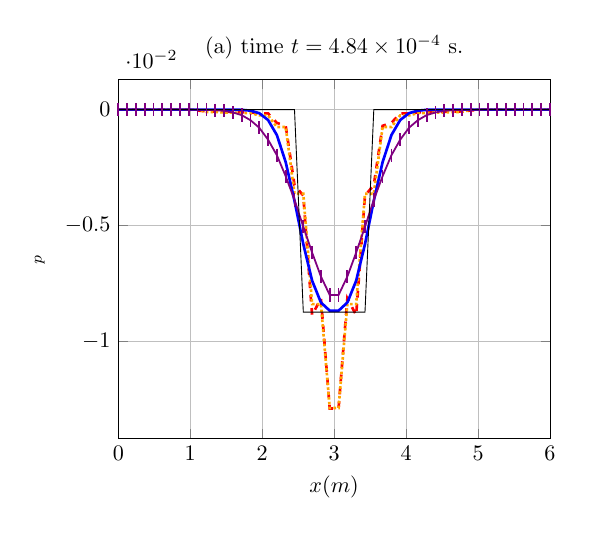
\begin{tikzpicture}[scale=0.8]
\begin{axis}[xlabel=$x (m)$,ylabel=$\eps^p$,ymajorgrids=true,xmajorgrids=true,legend pos=outer north east,title={(a) time $t = 4.84\times 10^{-4} $ s.},xmin=0.,xmax=6.]
\addplot[Red,very thick,mark=none,dashed,mark size=3pt] coordinates {(0.0,0.0) (0.12244897959183673,0.0) (0.24489795918367346,0.0) (0.36734693877551017,0.0) (0.4897959183673469,0.0) (0.6122448979591837,0.0) (0.7346938775510203,0.0) (0.8571428571428571,0.0) (0.9795918367346939,0.0) (1.1020408163265305,-3.791590211516079e-05) (1.2244897959183674,-7.70866275263142e-05) (1.346938775510204,-8.497586707829323e-05) (1.4693877551020407,-9.030872437715389e-05) (1.5918367346938775,-9.742060457186303e-05) (1.7142857142857142,-0.00011777294632526181) (1.836734693877551,-0.00011877997120884317) (1.9591836734693877,-0.00017229593911894644) (2.0816326530612246,-0.0001625095927714705) (2.204081632653061,-0.0005721718460187986) (2.326530612244898,-0.0006980928227095806) (2.4489795918367347,-0.003255684770391246) (2.571428571428571,-0.003703854150331533) (2.693877551020408,-0.008855536230217072) (2.816326530612245,-0.008134161982050364) (2.9387755102040813,-0.012877303196726952) (3.061224489795918,-0.012877303196726607) (3.183673469387755,-0.008134161982050527) (3.306122448979592,-0.008855536230216924) (3.4285714285714284,-0.00370385415033155) (3.5510204081632653,-0.0032556847703911866) (3.673469387755102,-0.0006980928227095723) (3.7959183673469385,-0.0005721718460187898) (3.9183673469387754,-0.0001625095927714674) (4.040816326530612,-0.00017229593911894956) (4.163265306122449,-0.00011877997120884148) (4.285714285714286,-0.00011777294632525957) (4.408163265306122,-9.74206045718636e-05) (4.530612244897959,-9.030872437715303e-05) (4.653061224489796,-8.497586707829776e-05) (4.775510204081632,-7.708662752631704e-05) (4.8979591836734695,-3.791590211516108e-05) (5.020408163265306,0.0) (5.142857142857142,0.0) (5.26530612244898,0.0) (5.387755102040816,0.0) (5.5102040816326525,0.0) (5.63265306122449,0.0) (5.755102040816326,0.0) (5.877551020408163,0.0) (6.0,0.0) };
\addplot[Orange,very thick,mark=none,densely dotted,mark size=3pt] coordinates {(0.0,0.0) (0.12244897959183673,0.0) (0.24489795918367346,0.0) (0.36734693877551017,0.0) (0.4897959183673469,0.0) (0.6122448979591837,0.0) (0.7346938775510203,0.0) (0.8571428571428571,0.0) (0.9795918367346939,0.0) (1.1020408163265305,0.0) (1.2244897959183674,-0.00010125340605535082) (1.346938775510204,-0.00010125340605535564) (1.4693877551020407,-0.00012349527304735526) (1.5918367346938775,-0.00012349527304735214) (1.7142857142857142,-0.0001510249264983643) (1.836734693877551,-0.0001510249264983569) (1.9591836734693877,-0.0002468617206963456) (2.0816326530612246,-0.00024686172069637857) (2.204081632653061,-0.0007504349417450695) (2.326530612244898,-0.0007504349417451243) (2.4489795918367347,-0.0036281593420660124) (2.571428571428571,-0.003628159342065948) (2.693877551020408,-0.008380076410022513) (2.816326530612245,-0.008380076410022256) (2.9387755102040813,-0.012853848358106693) (3.061224489795918,-0.0128538483581062) (3.183673469387755,-0.008380076410022525) (3.306122448979592,-0.008380076410022235) (3.4285714285714284,-0.003628159342066054) (3.5510204081632653,-0.00362815934206591) (3.673469387755102,-0.000750434941745111) (3.7959183673469385,-0.0007504349417450832) (3.9183673469387754,-0.00024686172069633743) (4.040816326530612,-0.00024686172069637695) (4.163265306122449,-0.00015102492649834897) (4.285714285714286,-0.0001510249264983674) (4.408163265306122,-0.00012349527304735949) (4.530612244897959,-0.00012349527304735412) (4.653061224489796,-0.00010125340605534598) (4.775510204081632,-0.00010125340605535762) (4.8979591836734695,0.0) (5.020408163265306,0.0) (5.142857142857142,0.0) (5.26530612244898,0.0) (5.387755102040816,0.0) (5.5102040816326525,0.0) (5.63265306122449,0.0) (5.755102040816326,0.0) (5.877551020408163,0.0) (6.0,0.0) };
\addplot[Blue,very thick,mark=none,solid,mark size=3pt] coordinates {(0.0,0.0) (0.12244897959183673,0.0) (0.24489795918367346,0.0) (0.36734693877551017,0.0) (0.4897959183673469,0.0) (0.6122448979591837,-5.222502208891369e-16) (0.7346938775510203,-3.801924841744559e-14) (0.8571428571428571,-1.3141666139875138e-12) (0.9795918367346939,-2.8745591924304055e-11) (1.1020408163265305,-4.464150179000128e-10) (1.2244897959183674,-5.23467841943105e-09) (1.346938775510204,-4.812046858639944e-08) (1.4693877551020407,-3.554036475964955e-07) (1.5918367346938775,-2.1443096765697003e-06) (1.7142857142857142,-1.0689498023182154e-05) (1.836734693877551,-4.436466051051049e-05) (1.9591836734693877,-0.00015404085928397946) (2.0816326530612246,-0.00044873332231471766) (2.204081632653061,-0.0010984305872627827) (2.326530612244898,-0.0022622254025038953) (2.4489795918367347,-0.003929978610103271) (2.571428571428571,-0.005797119893456445) (2.693877551020408,-0.007371043418348148) (2.816326530612245,-0.008310826779347521) (2.9387755102040813,-0.00866523151909913) (3.061224489795918,-0.008665231519099129) (3.183673469387755,-0.008310826779347523) (3.306122448979592,-0.007371043418348151) (3.4285714285714284,-0.0057971198934564485) (3.5510204081632653,-0.003929978610103277) (3.673469387755102,-0.002262225402503906) (3.7959183673469385,-0.0010984305872627934) (3.9183673469387754,-0.0004487333223147267) (4.040816326530612,-0.00015404085928398656) (4.163265306122449,-4.4364660510512195e-05) (4.285714285714286,-1.0689498023171936e-05) (4.408163265306122,-2.144309676557212e-06) (4.530612244897959,-3.554036475865614e-07) (4.653061224489796,-4.8120468574194675e-08) (4.775510204081632,-5.234678408361617e-09) (4.8979591836734695,-4.4641501165571666e-10) (5.020408163265306,-2.874559277579898e-11) (5.142857142857142,-1.314168884640648e-12) (5.26530612244898,-3.802009991237095e-14) (5.387755102040816,-5.242370423816499e-16) (5.5102040816326525,0.0) (5.63265306122449,0.0) (5.755102040816326,0.0) (5.877551020408163,0.0) (6.0,0.0) };
\addplot[Purple,thick,mark=|,solid,mark size=3pt] coordinates {(0.0,0.0) (0.12244897959183673,0.0) (0.24489795918367346,0.0) (0.36734693877551017,0.0) (0.4897959183673469,0.0) (0.6122448979591837,-8.792960346028919e-09) (0.7346938775510203,-3.786059785712333e-08) (0.8571428571428571,-2.508230825960636e-07) (0.9795918367346939,-8.265800991640205e-07) (1.1020408163265305,-3.1496141333668006e-06) (1.2244897959183674,-8.446763423661959e-06) (1.346938775510204,-2.3732282649803162e-05) (1.4693877551020407,-5.37012668957574e-05) (1.5918367346938775,-0.0001218346548242481) (1.7142857142857142,-0.00023802460823782993) (1.836734693877551,-0.0004559513032346254) (1.9591836734693877,-0.0007809726729771441) (2.0816326530612246,-0.001295399844018457) (2.204081632653061,-0.0019660778146380876) (2.326530612244898,-0.0028685788119150535) (2.4489795918367347,-0.0038889012981570665) (2.571428571428571,-0.005047541335664232) (2.693877551020408,-0.006159956990320315) (2.816326530612245,-0.007191476068263296) (2.9387755102040813,-0.007990368709145173) (3.061224489795918,-0.007990368709145174) (3.183673469387755,-0.007191476068263297) (3.306122448979592,-0.0061599569903203226) (3.4285714285714284,-0.005047541335664235) (3.5510204081632653,-0.003888901298157069) (3.673469387755102,-0.0028685788119150574) (3.7959183673469385,-0.001966077814638091) (3.9183673469387754,-0.0012953998440184578) (4.040816326530612,-0.0007809726729771479) (4.163265306122449,-0.0004559513032346283) (4.285714285714286,-0.00023802460823782627) (4.408163265306122,-0.00012183465482424442) (4.530612244897959,-5.3701266895754845e-05) (4.653061224489796,-2.3732282649791524e-05) (4.775510204081632,-8.446763423651173e-06) (4.8979591836734695,-3.1496141333639622e-06) (5.020408163265306,-8.265800991657234e-07) (5.142857142857142,-2.5082308259663124e-07) (5.26530612244898,-3.786059785967782e-08) (5.387755102040816,-8.79296034631275e-09) (5.5102040816326525,0.0) (5.63265306122449,0.0) (5.755102040816326,0.0) (5.877551020408163,0.0) (6.0,0.0) };
\addplot[black,thin,mark=none,solid,mark size=3pt] coordinates {(0.0,-0.0) (0.12244897959183673,-0.0) (0.24489795918367346,-0.0) (0.36734693877551017,-0.0) (0.4897959183673469,-0.0) (0.6122448979591837,-0.0) (0.7346938775510203,-0.0) (0.8571428571428571,-0.0) (0.9795918367346939,-0.0) (1.1020408163265305,-0.0) (1.2244897959183674,-0.0) (1.346938775510204,-0.0) (1.4693877551020407,-0.0) (1.5918367346938775,-0.0) (1.7142857142857142,-0.0) (1.836734693877551,-0.0) (1.9591836734693877,-0.0) (2.0816326530612246,-0.0) (2.204081632653061,-0.0) (2.326530612244898,-0.0) (2.4489795918367347,-0.0) (2.571428571428571,-0.008728715609439695) (2.693877551020408,-0.008728715609439695) (2.816326530612245,-0.008728715609439695) (2.9387755102040813,-0.008728715609439695) (3.061224489795918,-0.008728715609439695) (3.183673469387755,-0.008728715609439695) (3.306122448979592,-0.008728715609439695) (3.4285714285714284,-0.008728715609439695) (3.5510204081632653,-0.0) (3.673469387755102,-0.0) (3.7959183673469385,-0.0) (3.9183673469387754,-0.0) (4.040816326530612,-0.0) (4.163265306122449,-0.0) (4.285714285714286,-0.0) (4.408163265306122,-0.0) (4.530612244897959,-0.0) (4.653061224489796,-0.0) (4.775510204081632,-0.0) (4.8979591836734695,-0.0) (5.020408163265306,-0.0) (5.142857142857142,-0.0) (5.26530612244898,-0.0) (5.387755102040816,-0.0) (5.5102040816326525,-0.0) (5.63265306122449,-0.0) (5.755102040816326,-0.0) (5.877551020408163,-0.0) (6.0,-0.0) };
%\legend{usl,usf,dgmpm (ep solver),dgmpm (ac solver),exact}
\end{axis}
\end{tikzpicture}
%%% Local Variables:
%%% mode: latex
%%% TeX-master: "../../mainManuscript"
%%% End:
}
%   {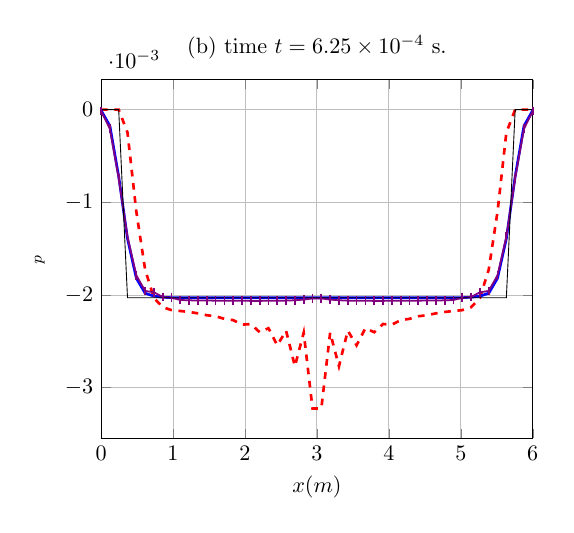
\begin{tikzpicture}[scale=0.8]
\begin{axis}[xlabel=$x (m)$,ylabel=$\eps^p$,ymajorgrids=true,xmajorgrids=true,legend pos=outer north east,title={(b) time $t = 6.25\times 10^{-4} $ s.},xmin=0.,xmax=6.]
\addplot[Red,very thick,mark=none,dashed] coordinates {(0.0,0.0) (0.12244897959183673,0.0) (0.24489795918367346,0.0) (0.36734693877551017,-0.0002478348228815541) (0.4897959183673469,-0.0011004378155012712) (0.6122448979591837,-0.0017260409269248597) (0.7346938775510203,-0.002031865332982762) (0.8571428571428571,-0.002132968518977378) (0.9795918367346939,-0.0021636018350532395) (1.1020408163265305,-0.0021733079916121177) (1.2244897959183674,-0.00218350748748031) (1.346938775510204,-0.002198645448466017) (1.4693877551020407,-0.002218920213241705) (1.5918367346938775,-0.002229697455331896) (1.7142857142857142,-0.002258121963594508) (1.836734693877551,-0.002271799079674154) (1.9591836734693877,-0.002320613632318322) (2.0816326530612246,-0.002313868472160546) (2.204081632653061,-0.0024020122032007017) (2.326530612244898,-0.0023588630990294623) (2.4489795918367347,-0.0025433455597807667) (2.571428571428571,-0.002385435935351422) (2.693877551020408,-0.0027693350417516906) (2.816326530612245,-0.0024065265204776445) (2.9387755102040813,-0.0032250612006492966) (3.061224489795918,-0.0032250612006492524) (3.183673469387755,-0.002406526520477666) (3.306122448979592,-0.0027693350417516823) (3.4285714285714284,-0.0023854359353514295) (3.5510204081632653,-0.0025433455597807628) (3.673469387755102,-0.002358863099029464) (3.7959183673469385,-0.0024020122032006983) (3.9183673469387754,-0.0023138684721605448) (4.040816326530612,-0.002320613632318319) (4.163265306122449,-0.0022717990796741546) (4.285714285714286,-0.0022581219635945077) (4.408163265306122,-0.0022296974553318956) (4.530612244897959,-0.0022189202132417056) (4.653061224489796,-0.0021986454484660173) (4.775510204081632,-0.0021835074874803095) (4.8979591836734695,-0.0021733079916121186) (5.020408163265306,-0.0021636018350532395) (5.142857142857142,-0.002132968518977378) (5.26530612244898,-0.002031865332982763) (5.387755102040816,-0.0017260409269248577) (5.5102040816326525,-0.0011004378155012658) (5.63265306122449,-0.0002478348228815494) (5.755102040816326,0.0) (5.877551020408163,0.0) (6.0,0.0) };
\addplot[Blue,very thick,mark=none,solid] coordinates {(0.0,-8.02367288935203e-06) (0.12244897959183673,-0.00017614426387335805) (0.24489795918367346,-0.0007207542691858686) (0.36734693877551017,-0.0013919930410856215) (0.4897959183673469,-0.001818355598439618) (0.6122448979591837,-0.001981300761387861) (0.7346938775510203,-0.0020125975551096974) (0.8571428571428571,-0.002024874952136019) (0.9795918367346939,-0.0020290867696967987) (1.1020408163265305,-0.002030353909504423) (1.2244897959183674,-0.0020306887880741907) (1.346938775510204,-0.0020307665725143873) (1.4693877551020407,-0.0020307824435747243) (1.5918367346938775,-0.0020307852835259937) (1.7142857142857142,-0.0020307857279245408) (1.836734693877551,-0.0020307857884822454) (1.9591836734693877,-0.00203078579562695) (2.0816326530612246,-0.002030785796351117) (2.204081632653061,-0.0020307857964135248) (2.326530612244898,-0.002030785796418031) (2.4489795918367347,-0.002030785796418302) (2.571428571428571,-0.0020307857964183135) (2.693877551020408,-0.002030785796418313) (2.816326530612245,-0.002030785796418313) (2.9387755102040813,-0.002030785796418314) (3.061224489795918,-0.0020307857964183135) (3.183673469387755,-0.0020307857964183135) (3.306122448979592,-0.0020307857964183126) (3.4285714285714284,-0.0020307857964183113) (3.5510204081632653,-0.0020307857964183005) (3.673469387755102,-0.002030785796418031) (3.7959183673469385,-0.0020307857964135217) (3.9183673469387754,-0.0020307857963511138) (4.040816326530612,-0.002030785795626948) (4.163265306122449,-0.0020307857884822433) (4.285714285714286,-0.0020307857279245403) (4.408163265306122,-0.0020307852835259915) (4.530612244897959,-0.0020307824435747226) (4.653061224489796,-0.0020307665725143842) (4.775510204081632,-0.002030688788074188) (4.8979591836734695,-0.0020303539095044196) (5.020408163265306,-0.0020290867696967953) (5.142857142857142,-0.0020248749521360144) (5.26530612244898,-0.0020125975551096966) (5.387755102040816,-0.0019813007613878565) (5.5102040816326525,-0.0018183555984396154) (5.63265306122449,-0.0013919930410856195) (5.755102040816326,-0.0007207542691858678) (5.877551020408163,-0.0001761442638733595) (6.0,-8.023672889353243e-06) };
\addplot[Purple,thick,mark=|,solid] coordinates {(0.0,-1.4376766038990375e-05) (0.12244897959183673,-0.0002078915703532438) (0.24489795918367346,-0.000740641579521879) (0.36734693877551017,-0.0013729886129224668) (0.4897959183673469,-0.001786873759629078) (0.6122448979591837,-0.0019568221398810824) (0.7346938775510203,-0.0019710253863315036) (0.8571428571428571,-0.002021925787657269) (0.9795918367346939,-0.00203043998544926) (1.1020408163265305,-0.002054595482920735) (1.2244897959183674,-0.0020576351166755064) (1.346938775510204,-0.0020609998518549564) (1.4693877551020407,-0.0020606031772355433) (1.5918367346938775,-0.002061501114574304) (1.7142857142857142,-0.002061887903336271) (1.836734693877551,-0.002062455598454706) (1.9591836734693877,-0.0020617923316583004) (2.0816326530612246,-0.002064203896841495) (2.204081632653061,-0.0020644266901542695) (2.326530612244898,-0.0020621094945296272) (2.4489795918367347,-0.002062767607181189) (2.571428571428571,-0.002061489252343496) (2.693877551020408,-0.0020573197208032658) (2.816326530612245,-0.0020502799029179) (2.9387755102040813,-0.0020377776694292327) (3.061224489795918,-0.0020377776694292327) (3.183673469387755,-0.002050279902917899) (3.306122448979592,-0.002057319720803265) (3.4285714285714284,-0.0020614892523434956) (3.5510204081632653,-0.0020627676071811878) (3.673469387755102,-0.0020621094945296285) (3.7959183673469385,-0.0020644266901542695) (3.9183673469387754,-0.0020642038968414953) (4.040816326530612,-0.0020617923316583004) (4.163265306122449,-0.002062455598454705) (4.285714285714286,-0.0020618879033362705) (4.408163265306122,-0.002061501114574307) (4.530612244897959,-0.0020606031772355464) (4.653061224489796,-0.002060999851854956) (4.775510204081632,-0.002057635116675507) (4.8979591836734695,-0.002054595482920736) (5.020408163265306,-0.002030439985449261) (5.142857142857142,-0.0020219257876572696) (5.26530612244898,-0.001971025386331503) (5.387755102040816,-0.0019568221398810802) (5.5102040816326525,-0.0017868737596290767) (5.63265306122449,-0.0013729886129224679) (5.755102040816326,-0.0007406415795218811) (5.877551020408163,-0.00020789157035324622) (6.0,-1.4376766038991588e-05) };
\addplot[black,thin,mark=none,solid] coordinates {(0.0,-0.0) (0.12244897959183673,-0.0) (0.24489795918367346,-0.0) (0.36734693877551017,-0.002030785796418313) (0.4897959183673469,-0.002030785796418313) (0.6122448979591837,-0.002030785796418313) (0.7346938775510203,-0.002030785796418313) (0.8571428571428571,-0.002030785796418313) (0.9795918367346939,-0.002030785796418313) (1.1020408163265305,-0.002030785796418313) (1.2244897959183674,-0.002030785796418313) (1.346938775510204,-0.002030785796418313) (1.4693877551020407,-0.002030785796418313) (1.5918367346938775,-0.002030785796418313) (1.7142857142857142,-0.002030785796418313) (1.836734693877551,-0.002030785796418313) (1.9591836734693877,-0.002030785796418313) (2.0816326530612246,-0.002030785796418313) (2.204081632653061,-0.002030785796418313) (2.326530612244898,-0.002030785796418313) (2.4489795918367347,-0.002030785796418313) (2.571428571428571,-0.002030785796418313) (2.693877551020408,-0.002030785796418313) (2.816326530612245,-0.002030785796418313) (2.9387755102040813,-0.002030785796418313) (3.061224489795918,-0.002030785796418313) (3.183673469387755,-0.002030785796418313) (3.306122448979592,-0.002030785796418313) (3.4285714285714284,-0.002030785796418313) (3.5510204081632653,-0.002030785796418313) (3.673469387755102,-0.002030785796418313) (3.7959183673469385,-0.002030785796418313) (3.9183673469387754,-0.002030785796418313) (4.040816326530612,-0.002030785796418313) (4.163265306122449,-0.002030785796418313) (4.285714285714286,-0.002030785796418313) (4.408163265306122,-0.002030785796418313) (4.530612244897959,-0.002030785796418313) (4.653061224489796,-0.002030785796418313) (4.775510204081632,-0.002030785796418313) (4.8979591836734695,-0.002030785796418313) (5.020408163265306,-0.002030785796418313) (5.142857142857142,-0.002030785796418313) (5.26530612244898,-0.002030785796418313) (5.387755102040816,-0.002030785796418313) (5.5102040816326525,-0.002030785796418313) (5.63265306122449,-0.002030785796418313) (5.755102040816326,-0.0) (5.877551020408163,-0.0) (6.0,-0.0) };
%\legend{usl 1ppc,dgmpm 1ppc (ep solver),dgmpm 1ppc (ac solver),exact}
\end{axis}
\end{tikzpicture}
%%% Local Variables:
%%% mode: latex
%%% TeX-master: "../../mainManuscript"
%%% End:
}
%   {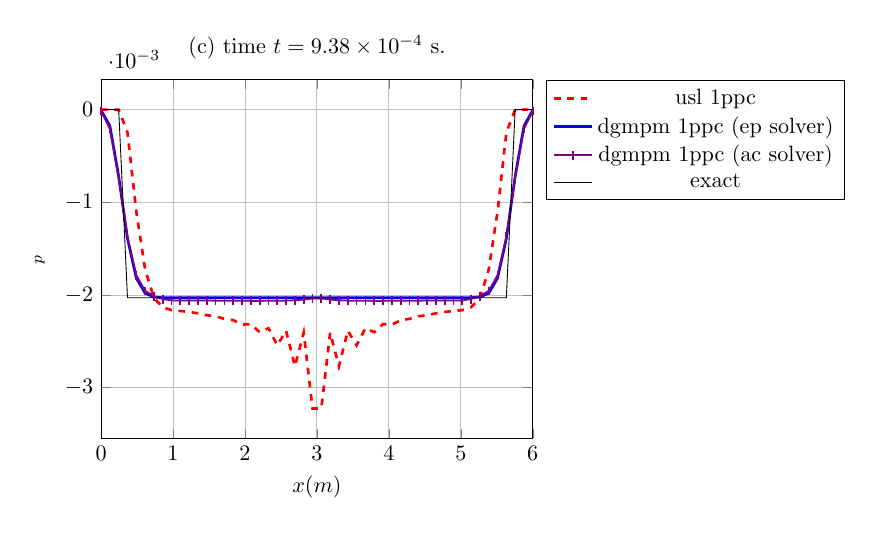
\begin{tikzpicture}[scale=0.8]
\begin{axis}[xlabel=$x (m)$,ylabel=$\eps^p$,ymajorgrids=true,xmajorgrids=true,legend pos=outer north east,title={(c) time $t = 9.38\times 10^{-4} $ s.},xmin=0.,xmax=6.]
\addplot[Red,very thick,mark=none,dashed] coordinates {(0.0,0.0) (0.12244897959183673,0.0) (0.24489795918367346,0.0) (0.36734693877551017,-0.0002478348228815541) (0.4897959183673469,-0.0011004378155012712) (0.6122448979591837,-0.0017260409269248597) (0.7346938775510203,-0.002031865332982762) (0.8571428571428571,-0.002132968518977378) (0.9795918367346939,-0.0021636018350532395) (1.1020408163265305,-0.0021733079916121177) (1.2244897959183674,-0.00218350748748031) (1.346938775510204,-0.002198645448466017) (1.4693877551020407,-0.002218920213241705) (1.5918367346938775,-0.002229697455331896) (1.7142857142857142,-0.002258121963594508) (1.836734693877551,-0.002271799079674154) (1.9591836734693877,-0.002320613632318322) (2.0816326530612246,-0.002313868472160546) (2.204081632653061,-0.0024020122032007017) (2.326530612244898,-0.0023588630990294623) (2.4489795918367347,-0.0025433455597807667) (2.571428571428571,-0.002385435935351422) (2.693877551020408,-0.0027693350417516906) (2.816326530612245,-0.0024065265204776445) (2.9387755102040813,-0.0032250612006492966) (3.061224489795918,-0.0032250612006492524) (3.183673469387755,-0.002406526520477666) (3.306122448979592,-0.0027693350417516823) (3.4285714285714284,-0.0023854359353514295) (3.5510204081632653,-0.0025433455597807628) (3.673469387755102,-0.002358863099029464) (3.7959183673469385,-0.0024020122032006983) (3.9183673469387754,-0.0023138684721605448) (4.040816326530612,-0.002320613632318319) (4.163265306122449,-0.0022717990796741546) (4.285714285714286,-0.0022581219635945077) (4.408163265306122,-0.0022296974553318956) (4.530612244897959,-0.0022189202132417056) (4.653061224489796,-0.0021986454484660173) (4.775510204081632,-0.0021835074874803095) (4.8979591836734695,-0.0021733079916121186) (5.020408163265306,-0.0021636018350532395) (5.142857142857142,-0.002132968518977378) (5.26530612244898,-0.002031865332982763) (5.387755102040816,-0.0017260409269248577) (5.5102040816326525,-0.0011004378155012658) (5.63265306122449,-0.0002478348228815494) (5.755102040816326,0.0) (5.877551020408163,0.0) (6.0,0.0) };
\addplot[Blue,very thick,mark=none,solid] coordinates {(0.0,-8.02367288935203e-06) (0.12244897959183673,-0.00017614426387335805) (0.24489795918367346,-0.0007207542691858686) (0.36734693877551017,-0.0013919930410856215) (0.4897959183673469,-0.001818355598439618) (0.6122448979591837,-0.001981300761387861) (0.7346938775510203,-0.0020224370921330336) (0.8571428571428571,-0.0020297345877472663) (0.9795918367346939,-0.0020306845407067867) (1.1020408163265305,-0.0020307781868908383) (1.2244897959183674,-0.002030785343345076) (1.346938775510204,-0.0020307857747949186) (1.4693877551020407,-0.002030785795584013) (1.5918367346938775,-0.0020307857963921434) (1.7142857142857142,-0.002030785796417646) (1.836734693877551,-0.0020307857964183005) (1.9591836734693877,-0.0020307857964183143) (2.0816326530612246,-0.002030785796418315) (2.204081632653061,-0.0020307857964183143) (2.326530612244898,-0.0020307857964183143) (2.4489795918367347,-0.002030785796418315) (2.571428571428571,-0.002030785796418316) (2.693877551020408,-0.0020307857964183143) (2.816326530612245,-0.0020307857964183143) (2.9387755102040813,-0.0020307857964183143) (3.061224489795918,-0.0020307857964183143) (3.183673469387755,-0.0020307857964183143) (3.306122448979592,-0.002030785796418315) (3.4285714285714284,-0.0020307857964183143) (3.5510204081632653,-0.002030785796418313) (3.673469387755102,-0.0020307857964183126) (3.7959183673469385,-0.0020307857964183126) (3.9183673469387754,-0.0020307857964183135) (4.040816326530612,-0.0020307857964183126) (4.163265306122449,-0.002030785796418296) (4.285714285714286,-0.002030785796417643) (4.408163265306122,-0.002030785796392141) (4.530612244897959,-0.002030785795584008) (4.653061224489796,-0.0020307857747949147) (4.775510204081632,-0.002030785343345074) (4.8979591836734695,-0.0020307781868908327) (5.020408163265306,-0.002030684540706785) (5.142857142857142,-0.0020297345877472632) (5.26530612244898,-0.0020224370921330275) (5.387755102040816,-0.0019813007613878565) (5.5102040816326525,-0.0018183555984396154) (5.63265306122449,-0.0013919930410856195) (5.755102040816326,-0.0007207542691858678) (5.877551020408163,-0.0001761442638733595) (6.0,-8.023672889353243e-06) };
\addplot[Purple,thick,mark=|,solid] coordinates {(0.0,-1.4376766038990375e-05) (0.12244897959183673,-0.0002078915703532438) (0.24489795918367346,-0.000740641579521879) (0.36734693877551017,-0.0013729886129224668) (0.4897959183673469,-0.001786873759629078) (0.6122448979591837,-0.0019568221398810824) (0.7346938775510203,-0.002012310558600745) (0.8571428571428571,-0.002044949844264105) (0.9795918367346939,-0.002058346964042081) (1.1020408163265305,-0.0020602219089299787) (1.2244897959183674,-0.0020610958163181556) (1.346938775510204,-0.0020609998518549564) (1.4693877551020407,-0.0020606031772355433) (1.5918367346938775,-0.002061501114574304) (1.7142857142857142,-0.002061887903336271) (1.836734693877551,-0.002062455598454706) (1.9591836734693877,-0.0020617923316583004) (2.0816326530612246,-0.002064203896841495) (2.204081632653061,-0.0020644266901542695) (2.326530612244898,-0.0020621094945296272) (2.4489795918367347,-0.002062767607181189) (2.571428571428571,-0.002061489252343496) (2.693877551020408,-0.0020573197208032658) (2.816326530612245,-0.0020502799029179) (2.9387755102040813,-0.0020377776694292327) (3.061224489795918,-0.0020377776694292327) (3.183673469387755,-0.002050279902917899) (3.306122448979592,-0.002057319720803265) (3.4285714285714284,-0.0020614892523434956) (3.5510204081632653,-0.0020627676071811878) (3.673469387755102,-0.0020621094945296285) (3.7959183673469385,-0.0020644266901542695) (3.9183673469387754,-0.0020642038968414953) (4.040816326530612,-0.0020617923316583004) (4.163265306122449,-0.002062455598454705) (4.285714285714286,-0.0020618879033362705) (4.408163265306122,-0.002061501114574307) (4.530612244897959,-0.0020606031772355464) (4.653061224489796,-0.002060999851854956) (4.775510204081632,-0.0020610958163181543) (4.8979591836734695,-0.002060221908929976) (5.020408163265306,-0.0020583469640420783) (5.142857142857142,-0.0020449498442641056) (5.26530612244898,-0.0020123105586007457) (5.387755102040816,-0.0019568221398810802) (5.5102040816326525,-0.0017868737596290767) (5.63265306122449,-0.0013729886129224679) (5.755102040816326,-0.0007406415795218811) (5.877551020408163,-0.00020789157035324622) (6.0,-1.4376766038991588e-05) };
\addplot[black,thin,mark=none,solid] coordinates {(0.0,-0.0) (0.12244897959183673,-0.0) (0.24489795918367346,-0.0) (0.36734693877551017,-0.002030785796418313) (0.4897959183673469,-0.002030785796418313) (0.6122448979591837,-0.002030785796418313) (0.7346938775510203,-0.002030785796418313) (0.8571428571428571,-0.002030785796418313) (0.9795918367346939,-0.002030785796418313) (1.1020408163265305,-0.002030785796418313) (1.2244897959183674,-0.002030785796418313) (1.346938775510204,-0.002030785796418313) (1.4693877551020407,-0.002030785796418313) (1.5918367346938775,-0.002030785796418313) (1.7142857142857142,-0.002030785796418313) (1.836734693877551,-0.002030785796418313) (1.9591836734693877,-0.002030785796418313) (2.0816326530612246,-0.002030785796418313) (2.204081632653061,-0.002030785796418313) (2.326530612244898,-0.002030785796418313) (2.4489795918367347,-0.002030785796418313) (2.571428571428571,-0.002030785796418313) (2.693877551020408,-0.002030785796418313) (2.816326530612245,-0.002030785796418313) (2.9387755102040813,-0.002030785796418313) (3.061224489795918,-0.002030785796418313) (3.183673469387755,-0.002030785796418313) (3.306122448979592,-0.002030785796418313) (3.4285714285714284,-0.002030785796418313) (3.5510204081632653,-0.002030785796418313) (3.673469387755102,-0.002030785796418313) (3.7959183673469385,-0.002030785796418313) (3.9183673469387754,-0.002030785796418313) (4.040816326530612,-0.002030785796418313) (4.163265306122449,-0.002030785796418313) (4.285714285714286,-0.002030785796418313) (4.408163265306122,-0.002030785796418313) (4.530612244897959,-0.002030785796418313) (4.653061224489796,-0.002030785796418313) (4.775510204081632,-0.002030785796418313) (4.8979591836734695,-0.002030785796418313) (5.020408163265306,-0.002030785796418313) (5.142857142857142,-0.002030785796418313) (5.26530612244898,-0.002030785796418313) (5.387755102040816,-0.002030785796418313) (5.5102040816326525,-0.002030785796418313) (5.63265306122449,-0.002030785796418313) (5.755102040816326,-0.0) (5.877551020408163,-0.0) (6.0,-0.0) };
\legend{usl 1ppc,dgmpm 1ppc (ep solver),dgmpm 1ppc (ac solver),exact}
\end{axis}
\end{tikzpicture}
%%% Local Variables:
%%% mode: latex
%%% TeX-master: "../../mainManuscript"
%%% End:
}
%   \caption{elastic-plastic RP epsp (1ppc)}
%   \label{fig:epsp_elastoplastic_RP}
% \end{figure}
% \begin{figure}[h!]
%   \centering
%   {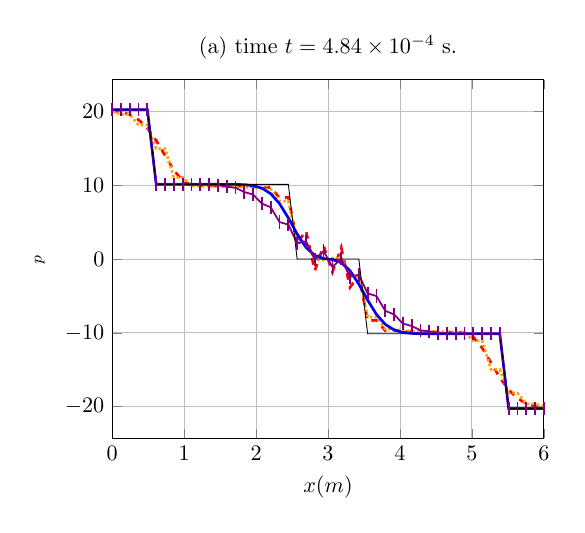
\begin{tikzpicture}[scale=0.8]
\begin{axis}[xlabel=$x (m)$,ylabel=$\eps^p$,ymajorgrids=true,xmajorgrids=true,legend pos=outer north east,title={(a) time $t = 4.84\times 10^{-4} $ s.},xmin=0.,xmax=6.]
\addplot[Red,very thick,mark=none,dashed,mark size=3pt] coordinates {(0.0,20.097963912667037) (0.12244897959183673,19.948200686683876) (0.24489795918367346,19.581623512332886) (0.36734693877551017,18.880401887543975) (0.4897959183673469,17.722027378885375) (0.6122448979591837,16.06462148503811) (0.7346938775510203,14.04922210395701) (0.8571428571428571,12.050777140391757) (0.9795918367346939,10.594448884991046) (1.1020408163265305,10.000299710369095) (1.2244897959183674,9.921016971597252) (1.346938775510204,9.905209334686656) (1.4693877551020407,9.897486036553882) (1.5918367346938775,9.881252793533395) (1.7142857142857142,9.874006895319209) (1.836734693877551,9.827852089496398) (1.9591836734693877,9.84660741015339) (2.0816326530612246,9.635377249359347) (2.204081632653061,9.703660809593103) (2.326530612244898,8.285921376176095) (2.4489795918367347,8.370712342612837) (2.571428571428571,2.1722672846759363) (2.693877551020408,3.830651803002166) (2.816326530612245,-1.5782561078814068) (2.9387755102040813,1.7774061156194738) (3.061224489795918,-1.777406115619491) (3.183673469387755,1.578256107881407) (3.306122448979592,-3.830651803002178) (3.4285714285714284,-2.172267284675949) (3.5510204081632653,-8.370712342612856) (3.673469387755102,-8.285921376176088) (3.7959183673469385,-9.703660809593108) (3.9183673469387754,-9.63537724935935) (4.040816326530612,-9.846607410153386) (4.163265306122449,-9.827852089496393) (4.285714285714286,-9.874006895319202) (4.408163265306122,-9.881252793533392) (4.530612244897959,-9.897486036553879) (4.653061224489796,-9.905209334686653) (4.775510204081632,-9.921016971597266) (4.8979591836734695,-10.000299710369097) (5.020408163265306,-10.594448884991042) (5.142857142857142,-12.05077714039174) (5.26530612244898,-14.049222103957007) (5.387755102040816,-16.064621485038092) (5.5102040816326525,-17.722027378885365) (5.63265306122449,-18.880401887543975) (5.755102040816326,-19.58162351233289) (5.877551020408163,-19.94820068668387) (6.0,-20.09796391266704) };
\addplot[Orange,very thick,mark=none,densely dotted,mark size=3pt] coordinates {(0.0,19.98524356533391) (0.12244897959183673,19.624972673600908) (0.24489795918367346,19.62497267360088) (0.36734693877551017,18.160148281550097) (0.4897959183673469,18.160148281550075) (0.6122448979591837,14.967460990115796) (0.7346938775510203,14.967460990115748) (0.8571428571428571,11.093523181440727) (0.9795918367346939,11.093523181440661) (1.1020408163265305,9.884184161534229) (1.2244897959183674,9.88418416153415) (1.346938775510204,9.848988655347343) (1.4693877551020407,9.848988655347272) (1.5918367346938775,9.805312262992565) (1.7142857142857142,9.805312262992501) (1.836734693877551,9.73354264540347) (1.9591836734693877,9.733542645403414) (2.0816326530612246,9.471881937395924) (2.204081632653061,9.471881937395832) (2.326530612244898,7.860641714627962) (2.4489795918367347,7.860641714627863) (2.571428571428571,2.220437432310992) (2.693877551020408,2.220437432310934) (2.816326530612245,-0.12736436093351383) (2.9387755102040813,-0.1273643609335115) (3.061224489795918,0.12736436093352144) (3.183673469387755,0.12736436093350467) (3.306122448979592,-2.220437432310998) (3.4285714285714284,-2.220437432310941) (3.5510204081632653,-7.860641714628002) (3.673469387755102,-7.860641714627828) (3.7959183673469385,-9.47188193739596) (3.9183673469387754,-9.471881937395791) (4.040816326530612,-9.733542645403523) (4.163265306122449,-9.73354264540336) (4.285714285714286,-9.805312262992585) (4.408163265306122,-9.805312262992468) (4.530612244897959,-9.848988655347373) (4.653061224489796,-9.848988655347233) (4.775510204081632,-9.884184161534241) (4.8979591836734695,-9.884184161534145) (5.020408163265306,-11.093523181440743) (5.142857142857142,-11.093523181440638) (5.26530612244898,-14.967460990115821) (5.387755102040816,-14.967460990115727) (5.5102040816326525,-18.1601482815501) (5.63265306122449,-18.16014828155006) (5.755102040816326,-19.624972673600908) (5.877551020408163,-19.62497267360089) (6.0,-19.985243565333896) };
\addplot[Blue,very thick,mark=none,solid,mark size=3pt] coordinates {(0.0,20.254787341673307) (0.12244897959183673,20.254787341673307) (0.24489795918367346,20.254787341673303) (0.36734693877551017,20.254787341673307) (0.4897959183673469,20.254787341673307) (0.6122448979591837,10.127393670836044) (0.7346938775510203,10.127393670792543) (0.8571428571428571,10.127393669311907) (0.9795918367346939,10.12739363748491) (1.1020408163265305,10.127393152888688) (1.2244897959183674,10.127387597360176) (1.346938775510204,10.127337839606644) (1.4693877551020407,10.1269813177698) (1.5918367346938775,10.124905759760324) (1.7142857142857142,10.114991301522732) (1.836734693877551,10.07592007470102) (1.9591836734693877,9.948669504170498) (2.0816326530612246,9.606755903306565) (2.204081632653061,8.852951991780422) (2.326530612244898,7.502672205682327) (2.4489795918367347,5.567680388456237) (2.571428571428571,3.401350808977297) (2.693877551020408,1.5752238210466734) (2.816326530612245,0.4848507939028141) (2.9387755102040813,0.07365669858902443) (3.061224489795918,-0.07365669858903101) (3.183673469387755,-0.48485079390282165) (3.306122448979592,-1.5752238210466838) (3.4285714285714284,-3.401350808977308) (3.5510204081632653,-5.56768038845625) (3.673469387755102,-7.502672205682339) (3.7959183673469385,-8.852951991780442) (3.9183673469387754,-9.606755903306581) (4.040816326530612,-9.948669504170525) (4.163265306122449,-10.075920074701049) (4.285714285714286,-10.11499130152276) (4.408163265306122,-10.124905759760349) (4.530612244897959,-10.126981317769818) (4.653061224489796,-10.12733783960665) (4.775510204081632,-10.127387597360173) (4.8979591836734695,-10.127393152888683) (5.020408163265306,-10.127393637484907) (5.142857142857142,-10.127393669311903) (5.26530612244898,-10.127393670792548) (5.387755102040816,-10.12739367083605) (5.5102040816326525,-20.25478734167332) (5.63265306122449,-20.254787341673318) (5.755102040816326,-20.25478734167332) (5.877551020408163,-20.25478734167332) (6.0,-20.254787341673314) };
\addplot[Purple,thick,mark=|,solid,mark size=3pt] coordinates {(0.0,20.254787341673307) (0.12244897959183673,20.254787341673307) (0.24489795918367346,20.254787341673303) (0.36734693877551017,20.254787341673307) (0.4897959183673469,20.254787341673307) (0.6122448979591837,10.127346919706891) (0.7346938775510203,10.12727737257173) (0.8571428571428571,10.126334047747402) (0.9795918367346939,10.125114755347433) (1.1020408163265305,10.11630010371687) (1.2244897959183674,10.106478421888186) (1.346938775510204,10.055869021868029) (1.4693877551020407,10.008062509066779) (1.5918367346938775,9.808511707883639) (1.7142857142857142,9.65367054792998) (1.836734693877551,9.082103441085764) (1.9591836734693877,8.739386895433114) (2.0816326530612246,7.513279145883331) (2.204081632653061,7.01727886939908) (2.326530612244898,5.014678544229133) (2.4489795918367347,4.663359241304864) (2.571428571428571,2.1468259041555218) (2.693877551020408,2.417528079544121) (2.816326530612245,-0.05847419216266908) (2.9387755102040813,1.0746179516287027) (3.061224489795918,-1.0746179516287169) (3.183673469387755,0.058474192162660144) (3.306122448979592,-2.417528079544138) (3.4285714285714284,-2.1468259041555355) (3.5510204081632653,-4.663359241304882) (3.673469387755102,-5.014678544229146) (3.7959183673469385,-7.017278869399091) (3.9183673469387754,-7.513279145883345) (4.040816326530612,-8.739386895433125) (4.163265306122449,-9.082103441085776) (4.285714285714286,-9.65367054792999) (4.408163265306122,-9.808511707883648) (4.530612244897959,-10.008062509066782) (4.653061224489796,-10.055869021868036) (4.775510204081632,-10.10647842188818) (4.8979591836734695,-10.11630010371688) (5.020408163265306,-10.125114755347425) (5.142857142857142,-10.12633404774741) (5.26530612244898,-10.127277372571715) (5.387755102040816,-10.127346919706907) (5.5102040816326525,-20.25478734167332) (5.63265306122449,-20.254787341673318) (5.755102040816326,-20.25478734167332) (5.877551020408163,-20.25478734167332) (6.0,-20.254787341673314) };
\addplot[black,thin,mark=none,solid,mark size=3pt] coordinates {(0.0,20.25478734167333) (0.12244897959183673,20.25478734167333) (0.24489795918367346,20.25478734167333) (0.36734693877551017,20.25478734167333) (0.4897959183673469,20.25478734167333) (0.6122448979591837,10.127393670836666) (0.7346938775510203,10.127393670836666) (0.8571428571428571,10.127393670836666) (0.9795918367346939,10.127393670836666) (1.1020408163265305,10.127393670836666) (1.2244897959183674,10.127393670836666) (1.346938775510204,10.127393670836666) (1.4693877551020407,10.127393670836666) (1.5918367346938775,10.127393670836666) (1.7142857142857142,10.127393670836666) (1.836734693877551,10.127393670836666) (1.9591836734693877,10.127393670836666) (2.0816326530612246,10.127393670836666) (2.204081632653061,10.127393670836666) (2.326530612244898,10.127393670836666) (2.4489795918367347,10.127393670836666) (2.571428571428571,-0.0) (2.693877551020408,-0.0) (2.816326530612245,-0.0) (2.9387755102040813,-0.0) (3.061224489795918,-0.0) (3.183673469387755,-0.0) (3.306122448979592,-0.0) (3.4285714285714284,-0.0) (3.5510204081632653,-10.127393670836666) (3.673469387755102,-10.127393670836666) (3.7959183673469385,-10.127393670836666) (3.9183673469387754,-10.127393670836666) (4.040816326530612,-10.127393670836666) (4.163265306122449,-10.127393670836666) (4.285714285714286,-10.127393670836666) (4.408163265306122,-10.127393670836666) (4.530612244897959,-10.127393670836666) (4.653061224489796,-10.127393670836666) (4.775510204081632,-10.127393670836666) (4.8979591836734695,-10.127393670836666) (5.020408163265306,-10.127393670836666) (5.142857142857142,-10.127393670836666) (5.26530612244898,-10.127393670836666) (5.387755102040816,-10.127393670836666) (5.5102040816326525,-20.25478734167333) (5.63265306122449,-20.25478734167333) (5.755102040816326,-20.25478734167333) (5.877551020408163,-20.25478734167333) (6.0,-20.25478734167333) };
%\legend{usl,usf,dgmpm (ep solver),dgmpm (ac solver),exact}
\end{axis}
\end{tikzpicture}
%%% Local Variables:
%%% mode: latex
%%% TeX-master: "../../mainManuscript"
%%% End:
}
%   {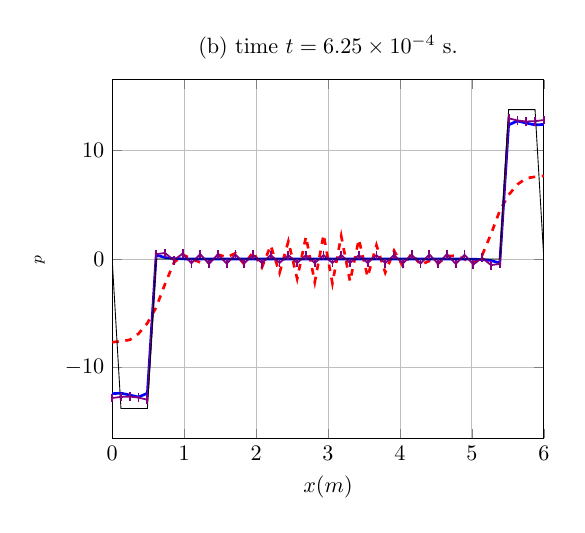
\begin{tikzpicture}[scale=0.8]
\begin{axis}[xlabel=$x (m)$,ylabel=$\eps^p$,ymajorgrids=true,xmajorgrids=true,legend pos=outer north east,title={(b) time $t = 6.25\times 10^{-4} $ s.},xmin=0.,xmax=6.]
\addplot[Red,very thick,mark=none,dashed] coordinates {(0.0,-7.656775715214294) (0.12244897959183673,-7.571339609307247) (0.24489795918367346,-7.438298117574187) (0.36734693877551017,-6.871029176921102) (0.4897959183673469,-5.903192627910385) (0.6122448979591837,-4.452057017543719) (0.7346938775510203,-2.3010481858807137) (0.8571428571428571,-0.3610443561643931) (0.9795918367346939,0.4188880742890505) (1.1020408163265305,0.01523876833598381) (1.2244897959183674,-0.3087249726610329) (1.346938775510204,-0.2682346195141458) (1.4693877551020407,0.41346894641452914) (1.5918367346938775,0.17204334381941044) (1.7142857142857142,0.5321881814826378) (1.836734693877551,-0.5074097815176064) (1.9591836734693877,0.6574508309639426) (2.0816326530612246,-0.7746969731901449) (2.204081632653061,1.2501366726613066) (2.326530612244898,-1.2807853076694733) (2.4489795918367347,1.631639383742251) (2.571428571428571,-1.8095691375383345) (2.693877551020408,2.0564749800644937) (2.816326530612245,-2.129190071354842) (2.9387755102040813,2.240060604992734) (3.061224489795918,-2.240060604992724) (3.183673469387755,2.1291900713548246) (3.306122448979592,-2.0564749800644746) (3.4285714285714284,1.809569137538315) (3.5510204081632653,-1.6316393837422516) (3.673469387755102,1.2807853076694653) (3.7959183673469385,-1.2501366726612742) (3.9183673469387754,0.7746969731901434) (4.040816326530612,-0.657450830963913) (4.163265306122449,0.5074097815175931) (4.285714285714286,-0.5321881814826224) (4.408163265306122,-0.17204334381940892) (4.530612244897959,-0.41346894641450627) (4.653061224489796,0.2682346195141527) (4.775510204081632,0.3087249726610414) (4.8979591836734695,-0.015238768335992692) (5.020408163265306,-0.4188880742890616) (5.142857142857142,0.3610443561643748) (5.26530612244898,2.3010481858807146) (5.387755102040816,4.452057017543711) (5.5102040816326525,5.90319262791038) (5.63265306122449,6.871029176921099) (5.755102040816326,7.4382981175741865) (5.877551020408163,7.571339609307248) (6.0,7.656775715214293) };
\addplot[Blue,very thick,mark=none,solid] coordinates {(0.0,-12.397952325377972) (0.12244897959183673,-12.346999574642966) (0.24489795918367346,-12.523092906128134) (0.36734693877551017,-12.71053547781855) (0.4897959183673469,-12.35049907311499) (0.6122448979591837,0.3722186738331613) (0.7346938775510203,0.1368090990556044) (0.8571428571428571,0.04446044382179651) (0.9795918367346939,0.012779812577704604) (1.1020408163265305,0.0032485856428356346) (1.2244897959183674,0.0007296815528062405) (1.346938775510204,0.00014459919089050038) (1.4693877551020407,2.5219563746036564e-05) (1.5918367346938775,3.857895635058131e-06) (1.7142857142857142,5.15199447901326e-07) (1.836734693877551,5.969388946802084e-08) (1.9591836734693877,5.952534698926585e-09) (2.0816326530612246,5.054662228331333e-10) (2.204081632653061,3.605726635043781e-11) (2.326530612244898,2.127654817367282e-12) (2.4489795918367347,1.1360160010621981e-13) (2.571428571428571,1.3411408617982763e-14) (2.693877551020408,1.66517088668301e-14) (2.816326530612245,5.526766510246074e-15) (2.9387755102040813,6.098792312826054e-15) (3.061224489795918,2.7682726724007426e-15) (3.183673469387755,7.175699018437728e-15) (3.306122448979592,-1.434813028923028e-14) (3.4285714285714284,-8.513769125527232e-15) (3.5510204081632653,-1.0095742773609699e-13) (3.673469387755102,-2.1199430888032018e-12) (3.7959183673469385,-3.6039619852103143e-11) (3.9183673469387754,-5.0545241703127e-10) (4.040816326530612,-5.9525221489037014e-09) (4.163265306122449,-5.969386814802888e-08) (4.285714285714286,-5.151994230605103e-07) (4.408163265306122,-3.8578956228878976e-06) (4.530612244897959,-2.5219563737562718e-05) (4.653061224489796,-0.00014459919087944834) (4.775510204081632,-0.0007296815527927886) (4.8979591836734695,-0.0032485856428289012) (5.020408163265306,-0.012779812577696097) (5.142857142857142,-0.04446044382178102) (5.26530612244898,-0.13680909905559333) (5.387755102040816,-0.3722186738331447) (5.5102040816326525,12.350499073115015) (5.63265306122449,12.71053547781857) (5.755102040816326,12.523092906128156) (5.877551020408163,12.346999574642979) (6.0,12.39795232537799) };
\addplot[Purple,thick,mark=|,solid] coordinates {(0.0,-12.795628373535159) (0.12244897959183673,-12.695543273778933) (0.24489795918367346,-12.666110940711564) (0.36734693877551017,-12.75241410003132) (0.4897959183673469,-12.960739789752774) (0.6122448979591837,0.44192323057668886) (0.7346938775510203,0.5605175207125453) (0.8571428571428571,-0.1118177278404644) (0.9795918367346939,0.49857571480888807) (1.1020408163265305,-0.3912177295445921) (1.2244897959183674,0.45869222504142426) (1.346938775510204,-0.4542184988816014) (1.4693877551020407,0.4392500135640788) (1.5918367346938775,-0.4268192827562814) (1.7142857142857142,0.4185270888397142) (1.836734693877551,-0.39693938041336063) (1.9591836734693877,0.398295251539175) (2.0816326530612246,-0.37211426798041747) (2.204081632653061,0.37593537352436907) (2.326530612244898,-0.3607380778681954) (2.4489795918367347,0.36132221537101705) (2.571428571428571,-0.3654682237983432) (2.693877551020408,0.35826901292698654) (2.816326530612245,-0.3691156051231741) (2.9387755102040813,0.36040411668068795) (3.061224489795918,-0.3604041166806867) (3.183673469387755,0.369115605123182) (3.306122448979592,-0.3582690129270081) (3.4285714285714284,0.36546822379836186) (3.5510204081632653,-0.3613222153709926) (3.673469387755102,0.3607380778681742) (3.7959183673469385,-0.37593537352436845) (3.9183673469387754,0.37211426798044456) (4.040816326530612,-0.3982952515391655) (4.163265306122449,0.3969393804133886) (4.285714285714286,-0.4185270888397233) (4.408163265306122,0.42681928275629366) (4.530612244897959,-0.43925001356404864) (4.653061224489796,0.45421849888160465) (4.775510204081632,-0.4586922250414254) (4.8979591836734695,0.3912177295446241) (5.020408163265306,-0.4985757148088702) (5.142857142857142,0.11181772784050628) (5.26530612244898,-0.560517520712548) (5.387755102040816,-0.4419232305766629) (5.5102040816326525,12.960739789752816) (5.63265306122449,12.75241410003134) (5.755102040816326,12.666110940711583) (5.877551020408163,12.695543273778958) (6.0,12.795628373535196) };
\addplot[black,thin,mark=none,solid] coordinates {(0.0,-0.0) (0.12244897959183673,-13.758687910475539) (0.24489795918367346,-13.758687910475539) (0.36734693877551017,-13.758687910475539) (0.4897959183673469,-13.758687910475539) (0.6122448979591837,-0.0) (0.7346938775510203,-0.0) (0.8571428571428571,-0.0) (0.9795918367346939,-0.0) (1.1020408163265305,-0.0) (1.2244897959183674,-0.0) (1.346938775510204,-0.0) (1.4693877551020407,-0.0) (1.5918367346938775,-0.0) (1.7142857142857142,-0.0) (1.836734693877551,-0.0) (1.9591836734693877,-0.0) (2.0816326530612246,-0.0) (2.204081632653061,-0.0) (2.326530612244898,-0.0) (2.4489795918367347,-0.0) (2.571428571428571,-0.0) (2.693877551020408,-0.0) (2.816326530612245,-0.0) (2.9387755102040813,-0.0) (3.061224489795918,-0.0) (3.183673469387755,-0.0) (3.306122448979592,-0.0) (3.4285714285714284,-0.0) (3.5510204081632653,-0.0) (3.673469387755102,-0.0) (3.7959183673469385,-0.0) (3.9183673469387754,-0.0) (4.040816326530612,-0.0) (4.163265306122449,-0.0) (4.285714285714286,-0.0) (4.408163265306122,-0.0) (4.530612244897959,-0.0) (4.653061224489796,-0.0) (4.775510204081632,-0.0) (4.8979591836734695,-0.0) (5.020408163265306,-0.0) (5.142857142857142,-0.0) (5.26530612244898,-0.0) (5.387755102040816,-0.0) (5.5102040816326525,13.758687910475539) (5.63265306122449,13.758687910475539) (5.755102040816326,13.758687910475539) (5.877551020408163,13.758687910475539) (6.0,0.0) };
%\legend{usl 1ppc,dgmpm 1ppc (ep solver),dgmpm 1ppc (ac solver),exact}
\end{axis}
\end{tikzpicture}
%%% Local Variables:
%%% mode: latex
%%% TeX-master: "../../mainManuscript"
%%% End:
}
%   {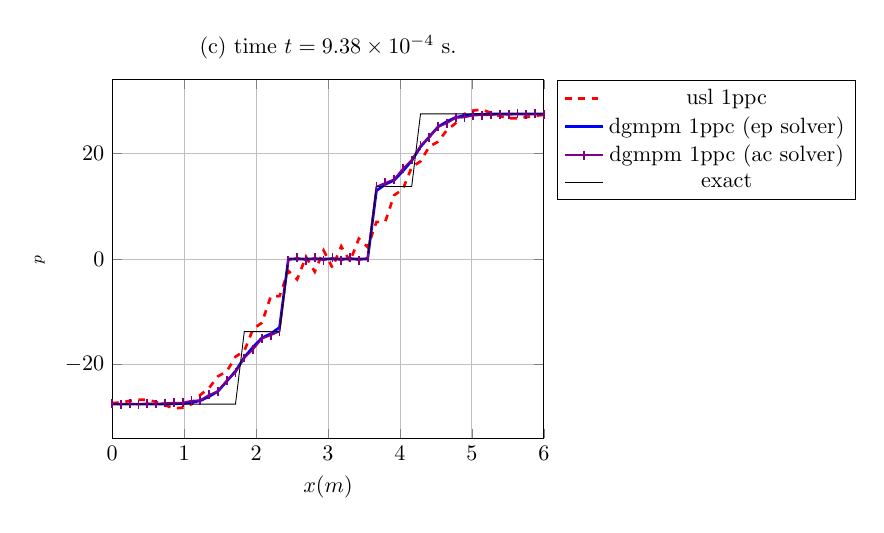
\begin{tikzpicture}[scale=0.8]
\begin{axis}[xlabel=$x (m)$,ylabel=$\eps^p$,ymajorgrids=true,xmajorgrids=true,legend pos=outer north east,title={(c) time $t = 9.38\times 10^{-4} $ s.},xmin=0.,xmax=6.]
\addplot[Red,very thick,mark=none,dashed] coordinates {(0.0,-27.331872449853556) (0.12244897959183673,-27.174400085417467) (0.24489795918367346,-26.904779830121768) (0.36734693877551017,-26.69301343005911) (0.4897959183673469,-26.683543140751915) (0.6122448979591837,-27.106963962300345) (0.7346938775510203,-27.704030887608354) (0.8571428571428571,-28.33906014232905) (0.9795918367346939,-28.167172814076366) (1.1020408163265305,-27.53334986092529) (1.2244897959183674,-25.775044707062726) (1.346938775510204,-24.466615882102165) (1.4693877551020407,-22.247186500301964) (1.5918367346938775,-21.33079179039491) (1.7142857142857142,-18.523714044368063) (1.836734693877551,-17.44233776410034) (1.9591836734693877,-13.237799741628182) (2.0816326530612246,-12.0894356407598) (2.204081632653061,-7.096371776087362) (2.326530612244898,-7.032925295785245) (2.4489795918367347,-2.2620897664972315) (2.571428571428571,-3.858668388515009) (2.693877551020408,0.4300541105363164) (2.816326530612245,-2.410115988529146) (2.9387755102040813,1.6326922086221445) (3.061224489795918,-1.6326922086221325) (3.183673469387755,2.410115988529122) (3.306122448979592,-0.43005411053631265) (3.4285714285714284,3.858668388514974) (3.5510204081632653,2.2620897664972395) (3.673469387755102,7.032925295785231) (3.7959183673469385,7.096371776087392) (3.9183673469387754,12.089435640759786) (4.040816326530612,13.237799741628214) (4.163265306122449,17.442337764100337) (4.285714285714286,18.523714044368088) (4.408163265306122,21.330791790394894) (4.530612244897959,22.247186500301982) (4.653061224489796,24.466615882102147) (4.775510204081632,25.775044707062744) (4.8979591836734695,27.53334986092529) (5.020408163265306,28.167172814076363) (5.142857142857142,28.33906014232903) (5.26530612244898,27.70403088760834) (5.387755102040816,27.106963962300348) (5.5102040816326525,26.683543140751933) (5.63265306122449,26.693013430059132) (5.755102040816326,26.904779830121797) (5.877551020408163,27.17440008541749) (6.0,27.331872449853574) };
\addplot[Blue,very thick,mark=none,solid] coordinates {(0.0,-27.517363397075158) (0.12244897959183673,-27.51732379155038) (0.24489795918367346,-27.517228936294842) (0.36734693877551017,-27.516689788484122) (0.4897959183673469,-27.51556852970287) (0.6122448979591837,-27.51025382248486) (0.7346938775510203,-27.500198710367762) (0.8571428571428571,-27.46081288016468) (0.9795918367346939,-27.394149463815687) (1.1020408163265305,-27.182111927326964) (1.2244897959183674,-26.86831399158136) (1.346938775510204,-26.07814929006618) (1.4693877551020407,-25.08839352872312) (1.5918367346938775,-23.189519000405884) (1.7142857142857142,-21.27348955232935) (1.836734693877551,-18.64183859399968) (1.9591836734693877,-16.67485639518814) (2.0816326530612246,-14.95207519835609) (2.204081632653061,-14.149762008703409) (2.326530612244898,-12.971197310204563) (2.4489795918367347,3.556080111931078e-14) (2.571428571428571,1.8614128550443383e-14) (2.693877551020408,1.1448988934369504e-14) (2.816326530612245,3.15403661725491e-14) (2.9387755102040813,2.1706952110207872e-14) (3.061224489795918,1.837643246978256e-14) (3.183673469387755,7.175699018437745e-15) (3.306122448979592,1.6868189305533344e-14) (3.4285714285714284,1.74998305367758e-14) (3.5510204081632653,1.3502410778036318e-14) (3.673469387755102,12.971197310204614) (3.7959183673469385,14.149762008703469) (3.9183673469387754,14.952075198356113) (4.040816326530612,16.67485639518816) (4.163265306122449,18.641838593999687) (4.285714285714286,21.273489552329384) (4.408163265306122,23.189519000405888) (4.530612244897959,25.088393528723138) (4.653061224489796,26.07814929006618) (4.775510204081632,26.868313991581342) (4.8979591836734695,27.182111927326957) (5.020408163265306,27.3941494638157) (5.142857142857142,27.46081288016466) (5.26530612244898,27.500198710367762) (5.387755102040816,27.51025382248485) (5.5102040816326525,27.515568529702865) (5.63265306122449,27.51668978848415) (5.755102040816326,27.517228936294806) (5.877551020408163,27.517323791550382) (6.0,27.517363397075165) };
\addplot[Purple,thick,mark=|,solid] coordinates {(0.0,-27.455491898583844) (0.12244897959183673,-27.52990791746212) (0.24489795918367346,-27.39669410111553) (0.36734693877551017,-27.56069772218648) (0.4897959183673469,-27.354208534961813) (0.6122448979591837,-27.484169218141297) (0.7346938775510203,-27.30529154707286) (0.8571428571428571,-27.260887430891447) (0.9795918367346939,-27.234362200737557) (1.1020408163265305,-26.87048565463221) (1.2244897959183674,-26.76603983934888) (1.346938775510204,-25.75807449243556) (1.4693877551020407,-25.06955937174821) (1.5918367346938775,-23.02673771458467) (1.7142857142857142,-21.509235536573875) (1.836734693877551,-18.773874989550777) (1.9591836734693877,-17.141311478227397) (2.0816326530612246,-15.098912535609557) (2.204081632653061,-14.451161421148855) (2.326530612244898,-13.715612700621918) (2.4489795918367347,-0.23693029878140853) (2.571428571428571,0.24220658661539068) (2.693877551020408,-0.22882318056987147) (2.816326530612245,0.2316928153217551) (2.9387755102040813,-0.22713962166300733) (3.061224489795918,0.22713962166305024) (3.183673469387755,-0.2316928153217785) (3.306122448979592,0.22882318056992768) (3.4285714285714284,-0.24220658661539307) (3.5510204081632653,0.23693029878141705) (3.673469387755102,13.71561270062201) (3.7959183673469385,14.451161421148875) (3.9183673469387754,15.098912535609603) (4.040816326530612,17.141311478227408) (4.163265306122449,18.77387498955077) (4.285714285714286,21.509235536573904) (4.408163265306122,23.026737714584694) (4.530612244897959,25.06955937174818) (4.653061224489796,25.758074492435522) (4.775510204081632,26.766039839348913) (4.8979591836734695,26.870485654632194) (5.020408163265306,27.23436220073757) (5.142857142857142,27.260887430891422) (5.26530612244898,27.305291547072898) (5.387755102040816,27.484169218141297) (5.5102040816326525,27.354208534961796) (5.63265306122449,27.560697722186475) (5.755102040816326,27.39669410111557) (5.877551020408163,27.529907917462097) (6.0,27.455491898583855) };
\addplot[black,thin,mark=none,solid] coordinates {(0.0,-27.517375820951077) (0.12244897959183673,-27.517375820951077) (0.24489795918367346,-27.517375820951077) (0.36734693877551017,-27.517375820951077) (0.4897959183673469,-27.517375820951077) (0.6122448979591837,-27.517375820951077) (0.7346938775510203,-27.517375820951077) (0.8571428571428571,-27.517375820951077) (0.9795918367346939,-27.517375820951077) (1.1020408163265305,-27.517375820951077) (1.2244897959183674,-27.517375820951077) (1.346938775510204,-27.517375820951077) (1.4693877551020407,-27.517375820951077) (1.5918367346938775,-27.517375820951077) (1.7142857142857142,-27.517375820951077) (1.836734693877551,-13.758687910475539) (1.9591836734693877,-13.758687910475539) (2.0816326530612246,-13.758687910475539) (2.204081632653061,-13.758687910475539) (2.326530612244898,-13.758687910475539) (2.4489795918367347,-0.0) (2.571428571428571,-0.0) (2.693877551020408,-0.0) (2.816326530612245,-0.0) (2.9387755102040813,-0.0) (3.061224489795918,-0.0) (3.183673469387755,-0.0) (3.306122448979592,-0.0) (3.4285714285714284,-0.0) (3.5510204081632653,-0.0) (3.673469387755102,13.758687910475539) (3.7959183673469385,13.758687910475539) (3.9183673469387754,13.758687910475539) (4.040816326530612,13.758687910475539) (4.163265306122449,13.758687910475539) (4.285714285714286,27.517375820951077) (4.408163265306122,27.517375820951077) (4.530612244897959,27.517375820951077) (4.653061224489796,27.517375820951077) (4.775510204081632,27.517375820951077) (4.8979591836734695,27.517375820951077) (5.020408163265306,27.517375820951077) (5.142857142857142,27.517375820951077) (5.26530612244898,27.517375820951077) (5.387755102040816,27.517375820951077) (5.5102040816326525,27.517375820951077) (5.63265306122449,27.517375820951077) (5.755102040816326,27.517375820951077) (5.877551020408163,27.517375820951077) (6.0,27.517375820951077) };
\legend{usl 1ppc,dgmpm 1ppc (ep solver),dgmpm 1ppc (ac solver),exact}
\end{axis}
\end{tikzpicture}
%%% Local Variables:
%%% mode: latex
%%% TeX-master: "../../mainManuscript"
%%% End:
}
%   \caption{elastic-plastic RP velo}
%   \label{fig:velo_elastoplastic_RP}
% \end{figure}


Comparison with mpm for 1ppc and 2ppcs with RK2 (requires additional bc treatment and constitutive). Only ep solver
%%%%%%%%%%%%%%%%%%%%%%%%%%%%%%%%%%%%%%%%%%%%%%%%%%%%%%%%%%%%%%%%%%%%%
% \begin{figure}[h!]
%   \centering
%   {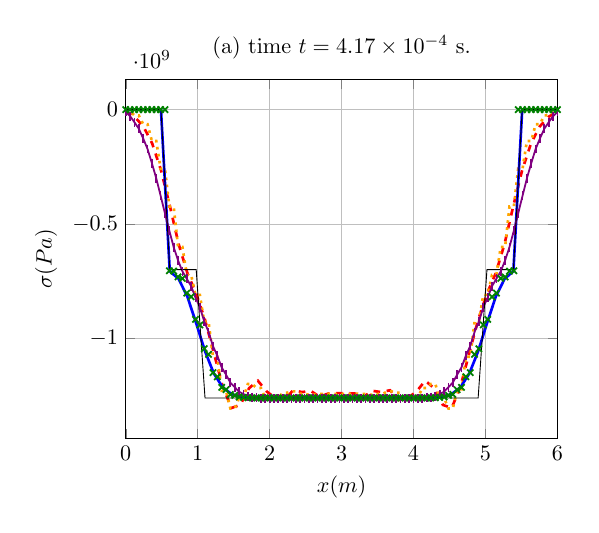
\begin{tikzpicture}[scale=0.8]
\begin{axis}[xlabel=$x (m)$,ylabel=$\sigma (Pa)$,ymajorgrids=true,xmajorgrids=true,legend pos=outer north east,title={(a) time $t = 4.17\times 10^{-4} $ s.},xmin=0.,xmax=6.]
\addplot[Red,very thick,mark=none,dashed] coordinates {(0.0,-8433215.03790355) (0.12244897959183673,-31379937.150059074) (0.24489795918367346,-73325965.87671247) (0.36734693877551017,-147815909.35881704) (0.4897959183673469,-264501011.32373637) (0.6122448979591837,-419797360.6339785) (0.7346938775510203,-586994803.1537646) (0.8571428571428571,-715242874.2277462) (0.9795918367346939,-804731796.1198385) (1.1020408163265305,-919403784.9173691) (1.2244897959183674,-1063504114.033879) (1.346938775510204,-1209904754.949398) (1.4693877551020407,-1304654513.0867395) (1.5918367346938775,-1291382612.5749428) (1.7142857142857142,-1218226204.6353252) (1.836734693877551,-1185455835.0777807) (1.9591836734693877,-1232745182.470082) (2.0816326530612246,-1261396271.0817113) (2.204081632653061,-1270103667.4391637) (2.326530612244898,-1227250869.598082) (2.4489795918367347,-1235273389.504192) (2.571428571428571,-1229787858.686364) (2.693877551020408,-1255621316.42765) (2.816326530612245,-1241442333.7811728) (2.9387755102040813,-1239848703.7218106) (3.061224489795918,-1239848703.7218091) (3.183673469387755,-1241442333.781176) (3.306122448979592,-1255621316.4276485) (3.4285714285714284,-1229787858.6863654) (3.5510204081632653,-1235273389.5041904) (3.673469387755102,-1227250869.598084) (3.7959183673469385,-1270103667.439164) (3.9183673469387754,-1261396271.081712) (4.040816326530612,-1232745182.4700806) (4.163265306122449,-1185455835.0777805) (4.285714285714286,-1218226204.6353254) (4.408163265306122,-1291382612.5749435) (4.530612244897959,-1304654513.0867395) (4.653061224489796,-1209904754.9493968) (4.775510204081632,-1063504114.033878) (4.8979591836734695,-919403784.917369) (5.020408163265306,-804731796.1198374) (5.142857142857142,-715242874.2277458) (5.26530612244898,-586994803.1537648) (5.387755102040816,-419797360.63397753) (5.5102040816326525,-264501011.3237358) (5.63265306122449,-147815909.35881624) (5.755102040816326,-73325965.8767119) (5.877551020408163,-31379937.150058918) (6.0,-8433215.037903389) };
\addplot[Orange,very thick,mark=none,dotted] coordinates {(0.0,-6487195.537951967) (0.06060606060606061,-6487195.537951967) (0.12121212121212122,-25447135.693615116) (0.18181818181818182,-25447135.693615116) (0.24242424242424243,-63824482.75083538) (0.30303030303030304,-63824482.75083538) (0.36363636363636365,-137285465.71899292) (0.42424242424242425,-137285465.71899292) (0.48484848484848486,-258389785.15975574) (0.5454545454545454,-258389785.15975574) (0.6060606060606061,-423881256.5395016) (0.6666666666666667,-423881256.5395016) (0.7272727272727273,-600583024.9453735) (0.7878787878787878,-600583024.9453735) (0.8484848484848485,-722865198.6395395) (0.9090909090909092,-722865198.6395395) (0.9696969696969697,-810023297.3770617) (1.0303030303030303,-810023297.3770617) (1.0909090909090908,-927952236.069318) (1.1515151515151516,-927952236.069318) (1.2121212121212122,-1080376380.893252) (1.2727272727272727,-1080376380.893252) (1.3333333333333335,-1229973271.6895852) (1.393939393939394,-1229973271.6895852) (1.4545454545454546,-1306874646.9216745) (1.5151515151515151,-1306874646.9216745) (1.5757575757575757,-1260590226.5138178) (1.6363636363636365,-1260590226.5138178) (1.696969696969697,-1200189199.3767865) (1.7575757575757576,-1200189199.3767865) (1.8181818181818183,-1217233767.7027068) (1.878787878787879,-1217233767.7027068) (1.9393939393939394,-1260358671.3727095) (2.0,-1260358671.3727095) (2.0606060606060606,-1261618284.922131) (2.121212121212121,-1261618284.922131) (2.1818181818181817,-1238228645.818687) (2.2424242424242427,-1238228645.818687) (2.303030303030303,-1232247837.5911345) (2.3636363636363638,-1232247837.5911345) (2.4242424242424243,-1242565564.7913089) (2.484848484848485,-1242565564.7913089) (2.5454545454545454,-1247187746.3284252) (2.606060606060606,-1247187746.3284252) (2.666666666666667,-1243527207.3601675) (2.7272727272727275,-1243527207.3601675) (2.787878787878788,-1241890915.1682148) (2.8484848484848486,-1241890915.1682148) (2.909090909090909,-1243871775.6139772) (2.9696969696969697,-1243871775.6139772) (3.0303030303030303,-1243871775.613977) (3.090909090909091,-1243871775.613977) (3.1515151515151514,-1241890915.1682146) (3.2121212121212124,-1241890915.1682146) (3.272727272727273,-1243527207.3601675) (3.3333333333333335,-1243527207.3601675) (3.393939393939394,-1247187746.3284254) (3.4545454545454546,-1247187746.3284254) (3.515151515151515,-1242565564.7913094) (3.5757575757575757,-1242565564.7913094) (3.6363636363636367,-1232247837.591135) (3.6969696969696972,-1232247837.591135) (3.757575757575758,-1238228645.818687) (3.8181818181818183,-1238228645.818687) (3.878787878787879,-1261618284.9221313) (3.9393939393939394,-1261618284.9221313) (4.0,-1260358671.37271) (4.0606060606060606,-1260358671.37271) (4.121212121212121,-1217233767.7027078) (4.181818181818182,-1217233767.7027078) (4.242424242424242,-1200189199.3767872) (4.303030303030303,-1200189199.3767872) (4.363636363636363,-1260590226.5138175) (4.424242424242425,-1260590226.5138175) (4.484848484848485,-1306874646.9216745) (4.545454545454546,-1306874646.9216745) (4.606060606060606,-1229973271.6895852) (4.666666666666667,-1229973271.6895852) (4.7272727272727275,-1080376380.893252) (4.787878787878788,-1080376380.893252) (4.848484848484849,-927952236.069318) (4.909090909090909,-927952236.069318) (4.96969696969697,-810023297.3770617) (5.03030303030303,-810023297.3770617) (5.090909090909091,-722865198.6395395) (5.151515151515151,-722865198.6395395) (5.212121212121212,-600583024.9453732) (5.2727272727272725,-600583024.9453732) (5.333333333333334,-423881256.5395015) (5.3939393939393945,-423881256.5395015) (5.454545454545455,-258389785.1597556) (5.515151515151516,-258389785.1597556) (5.575757575757576,-137285465.71899268) (5.636363636363637,-137285465.71899268) (5.696969696969697,-63824482.75083506) (5.757575757575758,-63824482.75083506) (5.818181818181818,-25447135.69361456) (5.878787878787879,-25447135.69361456) (5.9393939393939394,-6487195.537951966) (6.0,-6487195.537951966) };
\addplot[Blue,very thick,mark=none,solid] coordinates {(0.0,-3.2561158711216654e-07) (0.12244897959183673,-6.54162606232603e-22) (0.24489795918367346,0.0) (0.36734693877551017,3.2561158711216643e-07) (0.4897959183673469,-4.884173806682499e-07) (0.6122448979591837,-706703995.0062007) (0.7346938775510203,-739923853.3127105) (0.8571428571428571,-818114621.3278772) (0.9795918367346939,-934350667.0858994) (1.1020408163265305,-1056745717.4113452) (1.2244897959183674,-1153785079.176232) (1.346938775510204,-1213891661.9862223) (1.4693877551020407,-1243675875.166416) (1.5918367346938775,-1255667377.4619899) (1.7142857142857142,-1259628756.7765899) (1.836734693877551,-1260708382.472525) (1.9591836734693877,-1260951555.06527) (2.0816326530612246,-1260996741.6987677) (2.204081632653061,-1261003631.246593) (2.326530612244898,-1261004484.7294881) (2.4489795918367347,-1261004569.3136225) (2.571428571428571,-1261004575.8625927) (2.693877551020408,-1261004576.2443771) (2.816326530612245,-1261004576.2601426) (2.9387755102040813,-1261004576.2605536) (3.061224489795918,-1261004576.2605536) (3.183673469387755,-1261004576.2601426) (3.306122448979592,-1261004576.2443776) (3.4285714285714284,-1261004575.862593) (3.5510204081632653,-1261004569.3136227) (3.673469387755102,-1261004484.7294881) (3.7959183673469385,-1261003631.2465928) (3.9183673469387754,-1260996741.6987677) (4.040816326530612,-1260951555.0652697) (4.163265306122449,-1260708382.4725246) (4.285714285714286,-1259628756.7765894) (4.408163265306122,-1255667377.4619899) (4.530612244897959,-1243675875.1664157) (4.653061224489796,-1213891661.9862223) (4.775510204081632,-1153785079.176232) (4.8979591836734695,-1056745717.4113454) (5.020408163265306,-934350667.0858992) (5.142857142857142,-818114621.327877) (5.26530612244898,-739923853.3127109) (5.387755102040816,-706703995.0062011) (5.5102040816326525,-4.884173806682498e-07) (5.63265306122449,0.0) (5.755102040816326,-4.884173806682498e-07) (5.877551020408163,0.0) (6.0,-4.884173806682498e-07) };
\addplot[Purple,thick,mark=|,solid] coordinates {(0.0,-10397459.452423438) (0.06060606060606061,-28629486.986752886) (0.12121212121212122,-55131928.25663453) (0.18181818181818182,-83646270.11748616) (0.24242424242424243,-125654961.11636907) (0.30303030303030304,-172284594.0778725) (0.36363636363636365,-234043640.37607408) (0.42424242424242425,-300242328.04419184) (0.48484848484848486,-376432798.7765728) (0.5454545454545454,-453818751.237467) (0.6060606060606061,-529414416.2674847) (0.6666666666666667,-601300645.223565) (0.7272727272727273,-659382521.0565735) (0.7878787878787878,-707161316.1944203) (0.8484848484848485,-739803034.1794951) (0.9090909090909092,-772004069.950914) (0.9696969696969697,-822251842.2420584) (1.0303030303030303,-864154645.8439147) (1.0909090909090908,-925876995.0130453) (1.1515151515151516,-972279835.0233293) (1.2121212121212122,-1033743758.8085552) (1.2727272727272727,-1076108794.246372) (1.3333333333333335,-1126940545.3466995) (1.393939393939394,-1158983016.4555871) (1.4545454545454546,-1193843324.3931508) (1.5151515151515151,-1213855388.0055108) (1.5757575757575757,-1233610942.154643) (1.6363636363636365,-1243855259.0681229) (1.696969696969697,-1252984033.6395779) (1.7575757575757576,-1257191611.231863) (1.8181818181818183,-1260529554.0622826) (1.878787878787879,-1261847454.6142046) (1.9393939393939394,-1262731019.2058864) (2.0,-1262988692.0798318) (2.0606060606060606,-1263095211.659083) (2.121212121212121,-1263057284.7251215) (2.1818181818181817,-1263041880.329979) (2.2424242424242427,-1262967457.2713077) (2.303030303030303,-1262995543.9612422) (2.3636363636363638,-1262899504.1699014) (2.4242424242424243,-1262951100.2551603) (2.484848484848485,-1262880485.8465211) (2.5454545454545454,-1262941766.4492297) (2.606060606060606,-1262877340.9880557) (2.666666666666667,-1262975476.3750632) (2.7272727272727275,-1262864851.3501468) (2.787878787878788,-1263076922.0461023) (2.8484848484848486,-1262804308.8537025) (2.909090909090909,-1263257734.3780806) (2.9696969696969697,-1262658504.412126) (3.0303030303030303,-1262658504.4121263) (3.090909090909091,-1263257734.3780804) (3.1515151515151514,-1262804308.8537023) (3.2121212121212124,-1263076922.046102) (3.272727272727273,-1262864851.3501468) (3.3333333333333335,-1262975476.375064) (3.393939393939394,-1262877340.988056) (3.4545454545454546,-1262941766.4492295) (3.515151515151515,-1262880485.8465207) (3.5757575757575757,-1262951100.2551603) (3.6363636363636367,-1262899504.169902) (3.6969696969696972,-1262995543.961243) (3.757575757575758,-1262967457.2713082) (3.8181818181818183,-1263041880.329979) (3.878787878787879,-1263057284.7251215) (3.9393939393939394,-1263095211.6590827) (4.0,-1262988692.0798314) (4.0606060606060606,-1262731019.205886) (4.121212121212121,-1261847454.6142046) (4.181818181818182,-1260529554.0622826) (4.242424242424242,-1257191611.2318633) (4.303030303030303,-1252984033.6395783) (4.363636363636363,-1243855259.0681233) (4.424242424242425,-1233610942.1546435) (4.484848484848485,-1213855388.0055118) (4.545454545454546,-1193843324.3931518) (4.606060606060606,-1158983016.4555879) (4.666666666666667,-1126940545.3467004) (4.7272727272727275,-1076108794.2463727) (4.787878787878788,-1033743758.8085555) (4.848484848484849,-972279835.0233293) (4.909090909090909,-925876995.0130455) (4.96969696969697,-864154645.8439149) (5.03030303030303,-822251842.2420586) (5.090909090909091,-772004069.9509139) (5.151515151515151,-739803034.1794952) (5.212121212121212,-707161316.1944203) (5.2727272727272725,-659382521.0565742) (5.333333333333334,-601300645.2235655) (5.3939393939393945,-529414416.26748544) (5.454545454545455,-453818751.23746747) (5.515151515151516,-376432798.776573) (5.575757575757576,-300242328.0441918) (5.636363636363637,-234043640.37607414) (5.696969696969697,-172284594.0778724) (5.757575757575758,-125654961.1163687) (5.818181818181818,-83646270.11748542) (5.878787878787879,-55131928.256634116) (5.9393939393939394,-28629486.98675295) (6.0,-10397459.452423694) };
\addplot[Green,thick,mark=x,only marks] coordinates {(0.0,-9.938985241112485e-07) (0.06060606060606061,-1.2853825856739185e-06) (0.12121212121212122,8.201488924992559e-07) (0.18181818181818182,4.822974559494094e-07) (0.24242424242424243,-9.83648482392308e-07) (0.30303030303030304,-1.2956326273928566e-06) (0.36363636363636365,1.9586488831001813e-06) (0.42424242424242425,2.5999133364701503e-06) (0.48484848484848486,-1.4790882727589648e-06) (0.5454545454545454,-1.4514160112505328e-06) (0.6060606060606061,-704729842.2455659) (0.6666666666666667,-706002047.1314592) (0.7272727272727273,-731613409.0827894) (0.7878787878787878,-738307360.3254093) (0.8484848484848485,-802443845.4106181) (0.9090909090909092,-818702029.0002648) (0.9696969696969697,-917273418.4084023) (1.0303030303030303,-941457325.3246986) (1.0909090909090908,-1045498983.9435152) (1.1515151515151516,-1070147015.0174686) (1.2121212121212122,-1150104083.776542) (1.2727272727272727,-1168347225.6924338) (1.3333333333333335,-1214623647.0248165) (1.393939393939394,-1224762462.1158886) (1.4545454545454546,-1245337865.7733397) (1.5151515151515151,-1249651955.7951238) (1.5757575757575757,-1256756187.728854) (1.6363636363636365,-1258176137.8011208) (1.696969696969697,-1260087550.9276555) (1.7575757575757576,-1260449997.1780932) (1.8181818181818183,-1260849081.875068) (1.878787878787879,-1260920429.9830258) (1.9393939393939394,-1260984677.091578) (2.0,-1260995458.2161036) (2.0606060606060606,-1261002466.8790119) (2.121212121212121,-1261003454.0601096) (2.1818181818181817,-1261004228.03729) (2.2424242424242427,-1261004332.3287823) (2.303030303030303,-1261004658.4164412) (2.3636363636363638,-1261004353.5092869) (2.4242424242424243,-1261005248.8606844) (2.484848484848485,-1261004976.0401845) (2.5454545454545454,-1261004543.3087149) (2.606060606060606,-1261003848.6940825) (2.666666666666667,-1261005173.6392112) (2.7272727272727275,-1261003422.415637) (2.787878787878788,-1261005964.7480397) (2.8484848484848486,-1261003205.9507174) (2.909090909090909,-1261018212.4618385) (2.9696969696969697,-1260990356.2943678) (3.0303030303030303,-1260990356.2943668) (3.090909090909091,-1261018212.4618378) (3.1515151515151514,-1261003205.950717) (3.2121212121212124,-1261005964.7480397) (3.272727272727273,-1261003422.415637) (3.3333333333333335,-1261005173.6392105) (3.393939393939394,-1261003848.6940827) (3.4545454545454546,-1261004543.3087158) (3.515151515151515,-1261004976.0401855) (3.5757575757575757,-1261005248.860685) (3.6363636363636367,-1261004353.5092869) (3.6969696969696972,-1261004658.4164414) (3.757575757575758,-1261004332.328783) (3.8181818181818183,-1261004228.0372908) (3.878787878787879,-1261003454.0601094) (3.9393939393939394,-1261002466.8790114) (4.0,-1260995458.2161038) (4.0606060606060606,-1260984677.091578) (4.121212121212121,-1260920429.9830256) (4.181818181818182,-1260849081.8750677) (4.242424242424242,-1260449997.1780937) (4.303030303030303,-1260087550.9276562) (4.363636363636363,-1258176137.8011205) (4.424242424242425,-1256756187.728854) (4.484848484848485,-1249651955.795124) (4.545454545454546,-1245337865.7733407) (4.606060606060606,-1224762462.1158893) (4.666666666666667,-1214623647.024817) (4.7272727272727275,-1168347225.692434) (4.787878787878788,-1150104083.7765424) (4.848484848484849,-1070147015.0174688) (4.909090909090909,-1045498983.9435161) (4.96969696969697,-941457325.3246986) (5.03030303030303,-917273418.4084023) (5.090909090909091,-818702029.0002651) (5.151515151515151,-802443845.4106187) (5.212121212121212,-738307360.3254088) (5.2727272727272725,-731613409.0827891) (5.333333333333334,-706002047.1314601) (5.3939393939393945,-704729842.2455676) (5.454545454545455,-9.052507597537938e-07) (5.515151515151516,-7.228071758070392e-07) (5.575757575757576,8.567216523351019e-07) (5.636363636363637,7.713362832257307e-07) (5.696969696969697,-5.847958087280893e-07) (5.757575757575758,-7.176505397205777e-07) (5.818181818181818,1.1498742353244018e-06) (5.878787878787879,1.4550184615729307e-06) (5.9393939393939394,-2.547964815114839e-06) (6.0,-2.336208991567657e-06) };
\addplot[black,thin,mark=none,solid] coordinates {(0.0,-0.0) (0.12244897959183673,-0.0) (0.24489795918367346,-0.0) (0.36734693877551017,-0.0) (0.4897959183673469,-0.0) (0.6122448979591837,-700000000.0) (0.7346938775510203,-700000000.0) (0.8571428571428571,-700000000.0) (0.9795918367346939,-700000000.0) (1.1020408163265305,-1261004576.260559) (1.2244897959183674,-1261004576.260559) (1.346938775510204,-1261004576.260559) (1.4693877551020407,-1261004576.260559) (1.5918367346938775,-1261004576.260559) (1.7142857142857142,-1261004576.260559) (1.836734693877551,-1261004576.260559) (1.9591836734693877,-1261004576.260559) (2.0816326530612246,-1261004576.260559) (2.204081632653061,-1261004576.260559) (2.326530612244898,-1261004576.260559) (2.4489795918367347,-1261004576.260559) (2.571428571428571,-1261004576.260559) (2.693877551020408,-1261004576.260559) (2.816326530612245,-1261004576.260559) (2.9387755102040813,-1261004576.260559) (3.061224489795918,-1261004576.260559) (3.183673469387755,-1261004576.260559) (3.306122448979592,-1261004576.260559) (3.4285714285714284,-1261004576.260559) (3.5510204081632653,-1261004576.260559) (3.673469387755102,-1261004576.260559) (3.7959183673469385,-1261004576.260559) (3.9183673469387754,-1261004576.260559) (4.040816326530612,-1261004576.260559) (4.163265306122449,-1261004576.260559) (4.285714285714286,-1261004576.260559) (4.408163265306122,-1261004576.260559) (4.530612244897959,-1261004576.260559) (4.653061224489796,-1261004576.260559) (4.775510204081632,-1261004576.260559) (4.8979591836734695,-1261004576.260559) (5.020408163265306,-700000000.0) (5.142857142857142,-700000000.0) (5.26530612244898,-700000000.0) (5.387755102040816,-700000000.0) (5.5102040816326525,-0.0) (5.63265306122449,-0.0) (5.755102040816326,-0.0) (5.877551020408163,-0.0) (6.0,-0.0) };
%\legend{usl 1ppc,usl 2ppc,dgmpm 1ppc,dgmpm 2ppc,dgmpm 2ppc (RK2),exact}
\end{axis}
\end{tikzpicture}
%%% Local Variables:
%%% mode: latex
%%% TeX-master: "../../mainManuscript"
%%% End:
}
%   {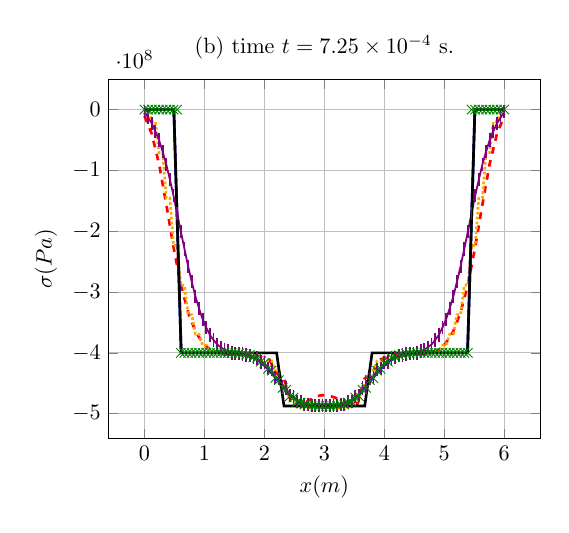
\begin{tikzpicture}[scale=0.8]
\begin{axis}[xlabel=$x (m)$,ylabel=$\sigma (Pa)$,ymajorgrids=true,xmajorgrids=true,legend pos=outer north east,title={(b) time $t = 7.25\times 10^{-4} $ s.}]
\addplot[Red,very thick,mark=none,dashed,mark size=3pt] coordinates {(0.0,-10477027.22040739) (0.12244897959183673,-40202439.77672757) (0.24489795918367346,-90268409.98400429) (0.36734693877551017,-157917330.96394995) (0.4897959183673469,-229098117.24026006) (0.6122448979591837,-290170966.79273176) (0.7346938775510203,-335449952.79523534) (0.8571428571428571,-366063963.8356788) (0.9795918367346939,-384934670.81956863) (1.1020408163265305,-394978768.22705775) (1.2244897959183674,-399539747.49342227) (1.346938775510204,-401064801.98949975) (1.4693877551020407,-401261686.3649931) (1.5918367346938775,-401362011.1717392) (1.7142857142857142,-402125702.7814173) (1.836734693877551,-402648608.50963366) (1.9591836734693877,-407517028.59914577) (2.0816326530612246,-411133976.99807984) (2.204081632653061,-433339939.374477) (2.326530612244898,-442099776.2163934) (2.4489795918367347,-483576545.68129754) (2.571428571428571,-481854124.4484605) (2.693877551020408,-481095256.73223835) (2.816326530612245,-473792554.1947772) (2.9387755102040813,-469732138.6842222) (3.061224489795918,-469732138.6842212) (3.183673469387755,-473792554.1947779) (3.306122448979592,-481095256.73223734) (3.4285714285714284,-481854124.4484616) (3.5510204081632653,-483576545.6812961) (3.673469387755102,-442099776.2163934) (3.7959183673469385,-433339939.3744765) (3.9183673469387754,-411133976.99807984) (4.040816326530612,-407517028.5991456) (4.163265306122449,-402648608.50963354) (4.285714285714286,-402125702.78141725) (4.408163265306122,-401362011.1717393) (4.530612244897959,-401261686.3649931) (4.653061224489796,-401064801.9894998) (4.775510204081632,-399539747.4934223) (4.8979591836734695,-394978768.22705775) (5.020408163265306,-384934670.81956846) (5.142857142857142,-366063963.83567846) (5.26530612244898,-335449952.79523504) (5.387755102040816,-290170966.7927308) (5.5102040816326525,-229098117.24025902) (5.63265306122449,-157917330.96394882) (5.755102040816326,-90268409.98400334) (5.877551020408163,-40202439.77672676) (6.0,-10477027.22040709) };
\addplot[Orange,very thick,mark=none,densely dotted,mark size=3pt] coordinates {(0.0,-1522322.3567553319) (0.06060606060606061,-1522322.3567553319) (0.12121212121212122,-19741546.758713853) (0.18181818181818182,-19741546.758713853) (0.24242424242424243,-70452847.74734518) (0.30303030303030304,-70452847.74734518) (0.36363636363636365,-145569726.72165304) (0.42424242424242425,-145569726.72165304) (0.48484848484848486,-223558621.35896367) (0.5454545454545454,-223558621.35896367) (0.6060606060606061,-288852526.8705149) (0.6666666666666667,-288852526.8705149) (0.7272727272727273,-337120167.47142065) (0.7878787878787878,-337120167.47142065) (0.8484848484848485,-369182466.2528492) (0.9090909090909092,-369182466.2528492) (0.9696969696969697,-387695734.7050902) (1.0303030303030303,-387695734.7050902) (1.0909090909090908,-396787746.7545124) (1.1515151515151516,-396787746.7545124) (1.2121212121212122,-400346482.5664338) (1.2727272727272727,-400346482.5664338) (1.3333333333333335,-401071106.301628) (1.393939393939394,-401071106.301628) (1.4545454545454546,-401189158.25601304) (1.5151515151515151,-401189158.25601304) (1.5757575757575757,-401411626.48080814) (1.6363636363636365,-401411626.48080814) (1.696969696969697,-401847412.82243955) (1.7575757575757576,-401847412.82243955) (1.8181818181818183,-402892812.90166867) (1.878787878787879,-402892812.90166867) (1.9393939393939394,-405871331.09740126) (2.0,-405871331.09740126) (2.0606060606060606,-413271912.46434987) (2.121212121212121,-413271912.46434987) (2.1818181818181817,-428650643.90280265) (2.2424242424242427,-428650643.90280265) (2.303030303030303,-453302573.20518476) (2.3636363636363638,-453302573.20518476) (2.4242424242424243,-478258276.212825) (2.484848484848485,-478258276.212825) (2.5454545454545454,-489476664.1834195) (2.606060606060606,-489476664.1834195) (2.666666666666667,-489046885.64068294) (2.7272727272727275,-489046885.64068294) (2.787878787878788,-491447894.73413926) (2.8484848484848486,-491447894.73413926) (2.909090909090909,-486436945.7103945) (2.9696969696969697,-486436945.7103945) (3.0303030303030303,-486436945.7103945) (3.090909090909091,-486436945.7103945) (3.1515151515151514,-491447894.73413926) (3.2121212121212124,-491447894.73413926) (3.272727272727273,-489046885.64068294) (3.3333333333333335,-489046885.64068294) (3.393939393939394,-489476664.1834195) (3.4545454545454546,-489476664.1834195) (3.515151515151515,-478258276.212825) (3.5757575757575757,-478258276.212825) (3.6363636363636367,-453302573.2051846) (3.6969696969696972,-453302573.2051846) (3.757575757575758,-428650643.9028025) (3.8181818181818183,-428650643.9028025) (3.878787878787879,-413271912.46434987) (3.9393939393939394,-413271912.46434987) (4.0,-405871331.09740126) (4.0606060606060606,-405871331.09740126) (4.121212121212121,-402892812.90166855) (4.181818181818182,-402892812.90166855) (4.242424242424242,-401847412.82243955) (4.303030303030303,-401847412.82243955) (4.363636363636363,-401411626.4808081) (4.424242424242425,-401411626.4808081) (4.484848484848485,-401189158.25601304) (4.545454545454546,-401189158.25601304) (4.606060606060606,-401071106.3016279) (4.666666666666667,-401071106.3016279) (4.7272727272727275,-400346482.5664337) (4.787878787878788,-400346482.5664337) (4.848484848484849,-396787746.75451225) (4.909090909090909,-396787746.75451225) (4.96969696969697,-387695734.7050903) (5.03030303030303,-387695734.7050903) (5.090909090909091,-369182466.25284934) (5.151515151515151,-369182466.25284934) (5.212121212121212,-337120167.47142065) (5.2727272727272725,-337120167.47142065) (5.333333333333334,-288852526.8705149) (5.3939393939393945,-288852526.8705149) (5.454545454545455,-223558621.35896364) (5.515151515151516,-223558621.35896364) (5.575757575757576,-145569726.72165304) (5.636363636363637,-145569726.72165304) (5.696969696969697,-70452847.74734521) (5.757575757575758,-70452847.74734521) (5.818181818181818,-19741546.758713897) (5.878787878787879,-19741546.758713897) (5.9393939393939394,-1522322.3567553656) (6.0,-1522322.3567553656) };
\addplot[Blue,very thick,mark=none,solid,mark size=3pt] coordinates {(0.0,-0.016398596440346053) (0.12244897959183673,-0.06425322857955201) (0.24489795918367346,-0.7380674881804443) (0.36734693877551017,-2.12047390173559) (0.4897959183673469,-28.76271861558054) (0.6122448979591837,-400000015.4159754) (0.7346938775510203,-400000102.7573024) (0.8571428571428571,-400000598.1932516) (0.9795918367346939,-400003055.79803795) (1.1020408163265305,-400013747.0436081) (1.2244897959183674,-400054602.7199052) (1.346938775510204,-400191823.2382515) (1.4693877551020407,-400596672.6802674) (1.5918367346938775,-401644186.51493835) (1.7142857142857142,-404014374.4754996) (1.836734693877551,-408684632.25449073) (1.9591836734693877,-416652037.9726774) (2.0816326530612246,-428329061.0045163) (2.204081632653061,-442879954.5361007) (2.326530612244898,-458084443.80872595) (2.4489795918367347,-471157539.9020842) (2.571428571428571,-480164339.19475454) (2.693877551020408,-484944715.5259052) (2.816326530612245,-486779650.5319825) (2.9387755102040813,-487233015.60471344) (3.061224489795918,-487233015.60471344) (3.183673469387755,-486779650.5319825) (3.306122448979592,-484944715.5259052) (3.4285714285714284,-480164339.19475454) (3.5510204081632653,-471157539.9020842) (3.673469387755102,-458084443.80872613) (3.7959183673469385,-442879954.5361007) (3.9183673469387754,-428329061.0045163) (4.040816326530612,-416652037.9726776) (4.163265306122449,-408684632.2544908) (4.285714285714286,-404014374.4754996) (4.408163265306122,-401644186.5149382) (4.530612244897959,-400596672.68026733) (4.653061224489796,-400191823.2382513) (4.775510204081632,-400054602.7199051) (4.8979591836734695,-400013747.04360807) (5.020408163265306,-400003055.79803795) (5.142857142857142,-400000598.19325155) (5.26530612244898,-400000102.75730234) (5.387755102040816,-400000015.4159754) (5.5102040816326525,-28.762718512303003) (5.63265306122449,-2.1204742438100417) (5.755102040816326,-0.7380675867576459) (5.877551020408163,-0.06425320166977637) (6.0,-0.01639854380134023) };
\addplot[Purple,thick,mark=|,solid,mark size=3pt] coordinates {(0.0,-3643722.4057531543) (0.06060606060606061,-13253871.94771175) (0.12121212121212122,-22430884.29879855) (0.18181818181818182,-35710388.05852378) (0.24242424242424243,-49954062.55465116) (0.30303030303030304,-69199724.63429566) (0.36363636363636365,-90001064.05703217) (0.42424242424242425,-115227809.11229268) (0.48484848484848486,-141771114.02793142) (0.5454545454545454,-170682311.90803242) (0.6060606060606061,-200079540.00258502) (0.6666666666666667,-229014826.8013297) (0.7272727272727273,-257430278.9843493) (0.7878787878787878,-282843592.21811193) (0.8484848484848485,-306971268.4010445) (0.9090909090909092,-326667104.7497092) (0.9696969696969697,-344782488.29979676) (1.0303030303030303,-358341830.7310785) (1.0909090909090908,-370462827.7146289) (1.1515151515151516,-378821810.49726343) (1.2121212121212122,-386102976.6619535) (1.2727272727272727,-390706555.81264853) (1.3333333333333335,-394846891.2394369) (1.393939393939394,-396879468.6459066) (1.4545454545454546,-400395334.89461267) (1.5151515151515151,-400547253.1901776) (1.5757575757575757,-401393994.5226969) (1.6363636363636365,-401653877.80383056) (1.696969696969697,-403469259.9494932) (1.7575757575757576,-403991527.1056523) (1.8181818181818183,-407625905.94533336) (1.878787878787879,-408563059.4680144) (1.9393939393939394,-414922856.8689467) (2.0,-416374885.2462252) (2.0606060606060606,-425987877.61701065) (2.121212121212121,-427906862.049074) (2.1818181818181817,-440309840.98849624) (2.2424242424242427,-442439362.1915814) (2.303030303030303,-455885132.24318355) (2.3636363636363638,-457826856.56220615) (2.4242424242424243,-469809715.6908375) (2.484848484848485,-471219084.61224025) (2.5454545454545454,-479722411.6158245) (2.606060606060606,-480495963.9518887) (2.666666666666667,-485058185.3772167) (2.7272727272727275,-485348110.0144077) (2.787878787878788,-487020339.6946885) (2.8484848484848486,-487075458.5679951) (2.909090909090909,-487055267.13670456) (2.9696969696969697,-486361892.7822711) (3.0303030303030303,-486361892.78227144) (3.090909090909091,-487055267.1367042) (3.1515151515151514,-487075458.5679951) (3.2121212121212124,-487020339.69468886) (3.272727272727273,-485348110.0144077) (3.3333333333333335,-485058185.37721705) (3.393939393939394,-480495963.9518887) (3.4545454545454546,-479722411.6158245) (3.515151515151515,-471219084.61224025) (3.5757575757575757,-469809715.6908375) (3.6363636363636367,-457826856.5622063) (3.6969696969696972,-455885132.24318355) (3.757575757575758,-442439362.1915814) (3.8181818181818183,-440309840.98849636) (3.878787878787879,-427906862.0490741) (3.9393939393939394,-425987877.6170107) (4.0,-416374885.2462253) (4.0606060606060606,-414922856.86894685) (4.121212121212121,-408563059.46801454) (4.181818181818182,-407625905.94533336) (4.242424242424242,-403991527.1056523) (4.303030303030303,-403469259.9494934) (4.363636363636363,-401653877.80383074) (4.424242424242425,-401393994.522697) (4.484848484848485,-400547253.19017774) (4.545454545454546,-400395334.89461285) (4.606060606060606,-396879468.6459065) (4.666666666666667,-394846891.23943704) (4.7272727272727275,-390706555.81264836) (4.787878787878788,-386102976.66195333) (4.848484848484849,-378821810.4972633) (4.909090909090909,-370462827.71462864) (4.96969696969697,-358341830.73107857) (5.03030303030303,-344782488.29979694) (5.090909090909091,-326667104.7497094) (5.151515151515151,-306971268.4010446) (5.212121212121212,-282843592.21811193) (5.2727272727272725,-257430278.98434916) (5.333333333333334,-229014826.8013294) (5.3939393939393945,-200079540.00258464) (5.454545454545455,-170682311.90803197) (5.515151515151516,-141771114.0279309) (5.575757575757576,-115227809.11229216) (5.636363636363637,-90001064.0570316) (5.696969696969697,-69199724.63429512) (5.757575757575758,-49954062.55465064) (5.818181818181818,-35710388.058523305) (5.878787878787879,-22430884.29879819) (5.9393939393939394,-13253871.947711527) (6.0,-3643722.4057530854) };
\addplot[Green,thin,mark=x,only marks,mark size=3pt] coordinates {(0.0,-0.0009905544907868183) (0.06060606060606061,-0.001035109508555422) (0.12121212121212122,-0.005117191018500656) (0.18181818181818182,-0.0052978434023460315) (0.24242424242424243,-0.06517986204950546) (0.30303030303030304,-0.07566277987844348) (0.36363636363636365,-0.24962042121048697) (0.42424242424242425,-0.26937038060136104) (0.48484848484848486,-3.010621421655401) (0.5454545454545454,-5.186761151690843) (0.6060606060606061,-400000002.01453906) (0.6666666666666667,-400000003.4473042) (0.7272727272727273,-400000017.3967542) (0.7878787878787878,-400000028.78236) (0.8484848484848485,-400000129.15230495) (0.9090909090909092,-400000206.4599203) (0.9696969696969697,-400000827.7884989) (1.0303030303030303,-400001277.7907757) (1.0909090909090908,-400004594.5128382) (1.1515151515151516,-400006844.3811263) (1.2121212121212122,-400022128.58005637) (1.2727272727272727,-400031796.16010183) (1.3333333333333335,-400092597.4804089) (1.393939393939394,-400128278.6945615) (1.4545454545454546,-400336842.6530185) (1.5151515151515151,-400449754.98737735) (1.5757575757575757,-401065298.1117383) (1.6363636363636365,-401370713.3108358) (1.696969696969697,-402928435.1963118) (1.7575757575757576,-403631417.36330265) (1.8181818181818183,-406995518.8189568) (1.878787878787879,-408364026.9334509) (1.9393939393939394,-414524891.6433188) (2.0,-416759867.3744382) (2.0606060606060606,-426248412.6400655) (2.121212121212121,-429277915.8940706) (2.1818181818181817,-441434961.5049247) (2.2424242424242427,-444795234.23076177) (2.303030303030303,-457568597.61163) (2.3636363636363638,-460560432.82157856) (2.4242424242424243,-471355976.94533) (2.484848484848485,-473437539.61930424) (2.5454545454545454,-480581531.6160863) (2.606060606060606,-481669280.4693011) (2.666666666666667,-485226958.9355893) (2.7272727272727275,-485627667.237451) (2.787878787878788,-486879003.35388845) (2.8484848484848486,-486971605.60944414) (2.909090909090909,-487248222.53163636) (2.9696969696969697,-487258302.19873005) (3.0303030303030303,-487258302.19873005) (3.090909090909091,-487248222.53163636) (3.1515151515151514,-486971605.60944414) (3.2121212121212124,-486879003.35388845) (3.272727272727273,-485627667.237451) (3.3333333333333335,-485226958.9355893) (3.393939393939394,-481669280.4693011) (3.4545454545454546,-480581531.6160863) (3.515151515151515,-473437539.6193044) (3.5757575757575757,-471355976.94533) (3.6363636363636367,-460560432.82157856) (3.6969696969696972,-457568597.61163) (3.757575757575758,-444795234.23076177) (3.8181818181818183,-441434961.5049247) (3.878787878787879,-429277915.8940706) (3.9393939393939394,-426248412.64006543) (4.0,-416759867.3744382) (4.0606060606060606,-414524891.64331895) (4.121212121212121,-408364026.933451) (4.181818181818182,-406995518.8189568) (4.242424242424242,-403631417.3633025) (4.303030303030303,-402928435.1963118) (4.363636363636363,-401370713.3108358) (4.424242424242425,-401065298.11173844) (4.484848484848485,-400449754.9873774) (4.545454545454546,-400336842.65301853) (4.606060606060606,-400128278.6945615) (4.666666666666667,-400092597.48040897) (4.7272727272727275,-400031796.16010183) (4.787878787878788,-400022128.5800565) (4.848484848484849,-400006844.3811263) (4.909090909090909,-400004594.51283836) (4.96969696969697,-400001277.7907758) (5.03030303030303,-400000827.7884989) (5.090909090909091,-400000206.4599203) (5.151515151515151,-400000129.152305) (5.212121212121212,-400000028.7823601) (5.2727272727272725,-400000017.39675426) (5.333333333333334,-400000003.4473042) (5.3939393939393945,-400000002.014539) (5.454545454545455,-5.186761729700046) (5.515151515151516,-3.0106210293278775) (5.575757575757576,-0.26937051997179645) (5.636363636363637,-0.249620419252184) (5.696969696969697,-0.07566313892965675) (5.757575757575758,-0.06517962792185199) (5.818181818181818,-0.00529745130538514) (5.878787878787879,-0.005117314055782253) (5.9393939393939394,-0.0010346801603060291) (6.0,-0.0009902966227138578) };
\addplot[black,very thick,mark=pentagone*,solid,mark size=3pt] coordinates {(0.0,-0.0) (0.12244897959183673,-0.0) (0.24489795918367346,-0.0) (0.36734693877551017,-0.0) (0.4897959183673469,-0.0) (0.6122448979591837,-400000000.0) (0.7346938775510203,-400000000.0) (0.8571428571428571,-400000000.0) (0.9795918367346939,-400000000.0) (1.1020408163265305,-400000000.0) (1.2244897959183674,-400000000.0) (1.346938775510204,-400000000.0) (1.4693877551020407,-400000000.0) (1.5918367346938775,-400000000.0) (1.7142857142857142,-400000000.0) (1.836734693877551,-400000000.0) (1.9591836734693877,-400000000.0) (2.0816326530612246,-400000000.0) (2.204081632653061,-400000000.0) (2.326530612244898,-487287156.09439695) (2.4489795918367347,-487287156.09439695) (2.571428571428571,-487287156.09439695) (2.693877551020408,-487287156.09439695) (2.816326530612245,-487287156.09439695) (2.9387755102040813,-487287156.09439695) (3.061224489795918,-487287156.09439695) (3.183673469387755,-487287156.09439695) (3.306122448979592,-487287156.09439695) (3.4285714285714284,-487287156.09439695) (3.5510204081632653,-487287156.09439695) (3.673469387755102,-487287156.09439695) (3.7959183673469385,-400000000.0) (3.9183673469387754,-400000000.0) (4.040816326530612,-400000000.0) (4.163265306122449,-400000000.0) (4.285714285714286,-400000000.0) (4.408163265306122,-400000000.0) (4.530612244897959,-400000000.0) (4.653061224489796,-400000000.0) (4.775510204081632,-400000000.0) (4.8979591836734695,-400000000.0) (5.020408163265306,-400000000.0) (5.142857142857142,-400000000.0) (5.26530612244898,-400000000.0) (5.387755102040816,-400000000.0) (5.5102040816326525,-0.0) (5.63265306122449,-0.0) (5.755102040816326,-0.0) (5.877551020408163,-0.0) (6.0,-0.0) };
%\legend{usl 1ppc,usl 2ppc,dgmpm 1ppc,dgmpm 2ppc,dgmpm 2ppc (RK2),exact}
\end{axis}
\end{tikzpicture}
%%% Local Variables:
%%% mode: latex
%%% TeX-master: "../../mainManuscript"
%%% End:
}
%   {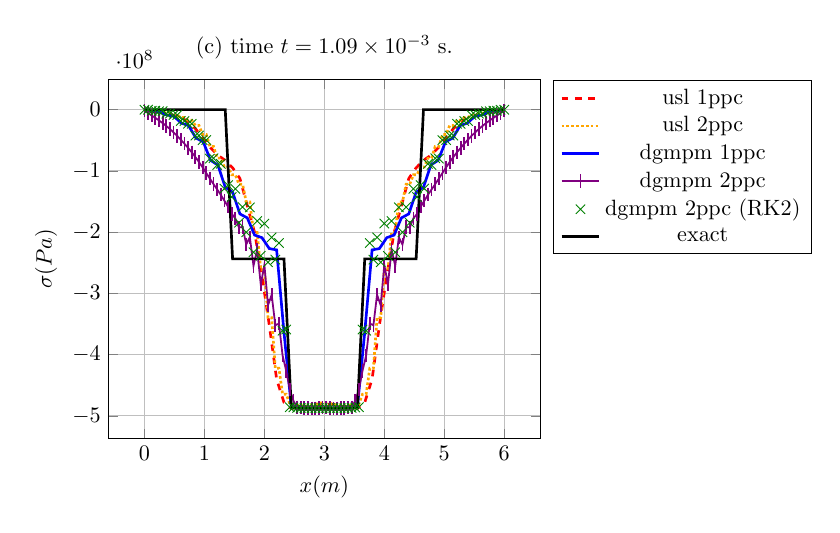
\begin{tikzpicture}[scale=0.8]
\begin{axis}[xlabel=$x (m)$,ylabel=$\sigma (Pa)$,ymajorgrids=true,xmajorgrids=true,legend pos=outer north east,title={(c) time $t = 1.09\times 10^{-3} $ s.}]
\addplot[Red,very thick,mark=none,dashed,mark size=3pt] coordinates {(0.0,-679166.0601331755) (0.12244897959183673,-2368189.594188208) (0.24489795918367346,-4606456.556212341) (0.36734693877551017,-6961578.395676694) (0.4897959183673469,-9332760.287028607) (0.6122448979591837,-12938682.464591796) (0.7346938775510203,-20102821.471402142) (0.8571428571428571,-32015823.341737133) (0.9795918367346939,-47676454.15860757) (1.1020408163265305,-62502940.42234602) (1.2244897959183674,-74544680.06037714) (1.346938775510204,-82775603.38522142) (1.4693877551020407,-94947363.4179823) (1.5918367346938775,-112415785.44002911) (1.7142857142857142,-156774491.63523546) (1.836734693877551,-200654618.50473383) (1.9591836734693877,-270646588.3413816) (2.0816326530612246,-351928629.9311485) (2.204081632653061,-440064160.15512294) (2.326530612244898,-477934424.91056436) (2.4489795918367347,-487815276.0764712) (2.571428571428571,-485351241.33413374) (2.693877551020408,-484406188.97201383) (2.816326530612245,-481035531.7602433) (2.9387755102040813,-481038509.8228564) (3.061224489795918,-481038509.8228558) (3.183673469387755,-481035531.7602443) (3.306122448979592,-484406188.9720135) (3.4285714285714284,-485351241.3341341) (3.5510204081632653,-487815276.07647014) (3.673469387755102,-477934424.9105651) (3.7959183673469385,-440064160.15512156) (3.9183673469387754,-351928629.931148) (4.040816326530612,-270646588.34138024) (4.163265306122449,-200654618.50473374) (4.285714285714286,-156774491.63523474) (4.408163265306122,-112415785.44002907) (4.530612244897959,-94947363.41798277) (4.653061224489796,-82775603.38522187) (4.775510204081632,-74544680.06037733) (4.8979591836734695,-62502940.42234604) (5.020408163265306,-47676454.158607304) (5.142857142857142,-32015823.341736842) (5.26530612244898,-20102821.471402) (5.387755102040816,-12938682.46459166) (5.5102040816326525,-9332760.287028512) (5.63265306122449,-6961578.395676572) (5.755102040816326,-4606456.55621225) (5.877551020408163,-2368189.594188123) (6.0,-679166.0601331636) };
\addplot[Orange,very thick,mark=none,densely dotted,mark size=3pt] coordinates {(0.0,-512829.37356199906) (0.06060606060606061,-512829.37356199906) (0.12121212121212122,-1685977.6907792736) (0.18181818181818182,-1685977.6907792736) (0.24242424242424243,-3409631.957049818) (0.30303030303030304,-3409631.957049818) (0.36363636363636365,-5994518.467970753) (0.42424242424242425,-5994518.467970753) (0.48484848484848486,-9186608.055434104) (0.5454545454545454,-9186608.055434104) (0.6060606060606061,-12632033.888351096) (0.6666666666666667,-12632033.888351096) (0.7272727272727273,-17308370.109125804) (0.7878787878787878,-17308370.109125804) (0.8484848484848485,-25927147.931033082) (0.9090909090909092,-25927147.931033082) (0.9696969696969697,-40719694.7337496) (1.0303030303030303,-40719694.7337496) (1.0909090909090908,-60222421.752752535) (1.1515151515151516,-60222421.752752535) (1.2121212121212122,-79232798.7243564) (1.2727272727272727,-79232798.7243564) (1.3333333333333335,-93917910.36545579) (1.393939393939394,-93917910.36545579) (1.4545454545454546,-106296964.05562654) (1.5151515151515151,-106296964.05562654) (1.5757575757575757,-121857025.50296684) (1.6363636363636365,-121857025.50296684) (1.696969696969697,-150591571.19633642) (1.7575757575757576,-150591571.19633642) (1.8181818181818183,-200655220.68880683) (1.878787878787879,-200655220.68880683) (1.9393939393939394,-261493503.50548327) (2.0,-261493503.50548327) (2.0606060606060606,-339524928.63039523) (2.121212121212121,-339524928.63039523) (2.1818181818181817,-422131801.353524) (2.2424242424242427,-422131801.353524) (2.303030303030303,-464494091.2915379) (2.3636363636363638,-464494091.2915379) (2.4242424242424243,-480288801.84594995) (2.484848484848485,-480288801.84594995) (2.5454545454545454,-482971319.0696361) (2.606060606060606,-482971319.0696361) (2.666666666666667,-484006263.5397973) (2.7272727272727275,-484006263.5397973) (2.787878787878788,-481823971.2401126) (2.8484848484848486,-481823971.2401126) (2.909090909090909,-478820708.8588188) (2.9696969696969697,-478820708.8588188) (3.0303030303030303,-478820708.8588188) (3.090909090909091,-478820708.8588188) (3.1515151515151514,-481823971.24011296) (3.2121212121212124,-481823971.24011296) (3.272727272727273,-484006263.53979766) (3.3333333333333335,-484006263.53979766) (3.393939393939394,-482971319.0696361) (3.4545454545454546,-482971319.0696361) (3.515151515151515,-480288801.84594995) (3.5757575757575757,-480288801.84594995) (3.6363636363636367,-464494091.2915379) (3.6969696969696972,-464494091.2915379) (3.757575757575758,-422131801.3535244) (3.8181818181818183,-422131801.3535244) (3.878787878787879,-339524928.6303949) (3.9393939393939394,-339524928.6303949) (4.0,-261493503.50548312) (4.0606060606060606,-261493503.50548312) (4.121212121212121,-200655220.68880683) (4.181818181818182,-200655220.68880683) (4.242424242424242,-150591571.1963363) (4.303030303030303,-150591571.1963363) (4.363636363636363,-121857025.50296697) (4.424242424242425,-121857025.50296697) (4.484848484848485,-106296964.05562642) (4.545454545454546,-106296964.05562642) (4.606060606060606,-93917910.36545563) (4.666666666666667,-93917910.36545563) (4.7272727272727275,-79232798.7243563) (4.787878787878788,-79232798.7243563) (4.848484848484849,-60222421.752752505) (4.909090909090909,-60222421.752752505) (4.96969696969697,-40719694.73374956) (5.03030303030303,-40719694.73374956) (5.090909090909091,-25927147.93103303) (5.151515151515151,-25927147.93103303) (5.212121212121212,-17308370.109125733) (5.2727272727272725,-17308370.109125733) (5.333333333333334,-12632033.888351053) (5.3939393939393945,-12632033.888351053) (5.454545454545455,-9186608.05543412) (5.515151515151516,-9186608.05543412) (5.575757575757576,-5994518.467970843) (5.636363636363637,-5994518.467970843) (5.696969696969697,-3409631.957049952) (5.757575757575758,-3409631.957049952) (5.818181818181818,-1685977.690779395) (5.878787878787879,-1685977.690779395) (5.9393939393939394,-512829.37356205017) (6.0,-512829.37356205017) };
\addplot[Blue,very thick,mark=none,solid,mark size=3pt] coordinates {(0.0,-298852.1952411225) (0.12244897959183673,-2592980.4740912793) (0.24489795918367346,-3560236.4322381816) (0.36734693877551017,-8652722.221047912) (0.4897959183673469,-10777216.673686886) (0.6122448979591837,-21974314.707157355) (0.7346938775510203,-26009924.918005344) (0.8571428571428571,-46347563.10657899) (0.9795918367346939,-52593345.171819046) (1.1020408163265305,-82683979.65035231) (1.2244897959183674,-90525380.97285904) (1.346938775510204,-126773557.44849168) (1.4693877551020407,-134743667.28836828) (1.5918367346938775,-170219249.4978279) (1.7142857142857142,-176744937.7749974) (1.836734693877551,-204799464.24688196) (1.9591836734693877,-209064122.25232974) (2.0816326530612246,-226820170.49378502) (2.204081632653061,-229011964.3130221) (2.326530612244898,-363270795.9137317) (2.4489795918367347,-485529213.90073514) (2.571428571428571,-486748760.1951447) (2.693877551020408,-487164866.56783277) (2.816326530612245,-487268871.16624963) (2.9387755102040813,-487285807.7274521) (3.061224489795918,-487285807.7274521) (3.183673469387755,-487268871.16624963) (3.306122448979592,-487164866.56783277) (3.4285714285714284,-486748760.1951447) (3.5510204081632653,-485529213.90073514) (3.673469387755102,-363270795.91372997) (3.7959183673469385,-229011964.3130223) (3.9183673469387754,-226820170.49378502) (4.040816326530612,-209064122.25232938) (4.163265306122449,-204799464.2468816) (4.285714285714286,-176744937.77499697) (4.408163265306122,-170219249.4978276) (4.530612244897959,-134743667.28836808) (4.653061224489796,-126773557.44849148) (4.775510204081632,-90525380.9728589) (4.8979591836734695,-82683979.65035222) (5.020408163265306,-52593345.171819076) (5.142857142857142,-46347563.10657902) (5.26530612244898,-26009924.918005634) (5.387755102040816,-21974314.707157686) (5.5102040816326525,-10777216.673687106) (5.63265306122449,-8652722.22104813) (5.755102040816326,-3560236.4322383474) (5.877551020408163,-2592980.4740913147) (6.0,-298852.1952412414) };
\addplot[Purple,thick,mark=|,solid,mark size=3pt] coordinates {(0.0,-1967506.1700863338) (0.06060606060606061,-5640032.662143143) (0.12121212121212122,-9656978.414919749) (0.18181818181818182,-13511820.529648876) (0.24242424242424243,-17791285.14768848) (0.30303030303030304,-22020954.760085706) (0.36363636363636365,-26810841.63481511) (0.42424242424242425,-31669769.847401485) (0.48484848484848486,-37219038.25874583) (0.5454545454545454,-42898302.86376866) (0.6060606060606061,-49215331.978578255) (0.6666666666666667,-55631508.92977342) (0.7272727272727273,-62575105.835719146) (0.7878787878787878,-69650368.30460997) (0.8484848484848485,-77440912.11382866) (0.9090909090909092,-85513317.74757525) (0.9696969696969697,-94394406.18118168) (1.0303030303030303,-103458727.33292748) (1.0909090909090908,-112622821.36245859) (1.1515151515151516,-121624138.89888178) (1.2121212121212122,-130341670.55898608) (1.2727272727272727,-139154542.84528217) (1.3333333333333335,-148830679.63128546) (1.393939393939394,-158542307.8017911) (1.4545454545454546,-170175255.01202118) (1.5151515151515151,-177512130.9706464) (1.5757575757575757,-192468554.83417034) (1.6363636363636365,-191410973.67950493) (1.696969696969697,-220188643.16229337) (1.7575757575757576,-208348179.3812332) (1.8181818181818183,-255105244.69638902) (1.878787878787879,-228761423.37895402) (1.9393939393939394,-285472179.8898197) (2.0,-253525121.96460363) (2.0606060606060606,-319389070.9725514) (2.121212121212121,-302097367.51271814) (2.1818181818181817,-351940004.91030246) (2.2424242424242427,-349259097.20874596) (2.303030303030303,-401088439.8898511) (2.3636363636363638,-426445036.100153) (2.4242424242424243,-456776041.9007156) (2.484848484848485,-475327504.30100346) (2.5454545454545454,-485932720.49084026) (2.606060606060606,-486800863.6836889) (2.666666666666667,-487206914.08181626) (2.7272727272727275,-487221866.2556566) (2.787878787878788,-487293102.56783485) (2.8484848484848486,-487291983.48275816) (2.909090909090909,-486820130.2994909) (2.9696969696969697,-486154460.1484115) (3.0303030303030303,-486154460.1484115) (3.090909090909091,-486820130.2994909) (3.1515151515151514,-487291983.4827589) (3.2121212121212124,-487293102.56783485) (3.272727272727273,-487221866.2556566) (3.3333333333333335,-487206914.08181626) (3.393939393939394,-486800863.68368924) (3.4545454545454546,-485932720.4908413) (3.515151515151515,-475327504.30100375) (3.5757575757575757,-456776041.90071523) (3.6363636363636367,-426445036.10015374) (3.6969696969696972,-401088439.8898514) (3.757575757575758,-349259097.2087466) (3.8181818181818183,-351940004.91030276) (3.878787878787879,-302097367.5127176) (3.9393939393939394,-319389070.9725512) (4.0,-253525121.96460345) (4.0606060606060606,-285472179.8898196) (4.121212121212121,-228761423.3789541) (4.181818181818182,-255105244.69638902) (4.242424242424242,-208348179.3812334) (4.303030303030303,-220188643.16229364) (4.363636363636363,-191410973.6795053) (4.424242424242425,-192468554.83417064) (4.484848484848485,-177512130.97064662) (4.545454545454546,-170175255.01202148) (4.606060606060606,-158542307.8017913) (4.666666666666667,-148830679.63128573) (4.7272727272727275,-139154542.84528223) (4.787878787878788,-130341670.55898641) (4.848484848484849,-121624138.89888197) (4.909090909090909,-112622821.36245887) (4.96969696969697,-103458727.33292772) (5.03030303030303,-94394406.18118192) (5.090909090909091,-85513317.74757543) (5.151515151515151,-77440912.11382888) (5.212121212121212,-69650368.30461016) (5.2727272727272725,-62575105.83571933) (5.333333333333334,-55631508.92977359) (5.3939393939393945,-49215331.97857844) (5.454545454545455,-42898302.863768816) (5.515151515151516,-37219038.25874599) (5.575757575757576,-31669769.847401626) (5.636363636363637,-26810841.634815253) (5.696969696969697,-22020954.760085825) (5.757575757575758,-17791285.147688594) (5.818181818181818,-13511820.529648978) (5.878787878787879,-9656978.414919829) (5.9393939393939394,-5640032.662143192) (6.0,-1967506.1700863515) };
\addplot[Green,thin,mark=x,only marks,mark size=3pt] coordinates {(0.0,-230769.40948159585) (0.06060606060606061,-230768.71951221325) (0.12121212121212122,-1765050.39034623) (0.18181818181818182,-1765048.7256776437) (0.24242424242424243,-2617614.5488237087) (0.30303030303030304,-2617595.5576229785) (0.36363636363636365,-6618855.725385412) (0.42424242424242425,-6618791.381126346) (0.48484848484848486,-8782768.896716146) (0.5454545454545454,-8782347.865813052) (0.6060606060606061,-18621957.945415) (0.6666666666666667,-18620353.83429409) (0.7272727272727273,-23151239.305377506) (0.7878787878787878,-23143055.39749537) (0.8484848484848485,-42429548.36143795) (0.9090909090909092,-42396573.934735104) (0.9696969696969697,-49952758.0967802) (1.0303030303030303,-49806565.98801953) (1.0909090909090908,-80012587.42975214) (1.1515151515151516,-79461376.35879174) (1.2121212121212122,-90415119.5727169) (1.2727272727272727,-88488293.78873543) (1.3333333333333335,-128889020.76572785) (1.393939393939394,-123386634.02232555) (1.4545454545454546,-142761259.00417286) (1.5151515151515151,-129449157.87721576) (1.5757575757575757,-184648477.15027985) (1.6363636363636365,-158996250.14018014) (1.696969696969697,-200285677.94521412) (1.7575757575757576,-159431830.86237475) (1.8181818181818183,-232788597.47549) (1.878787878787879,-181815073.16887435) (1.9393939393939394,-238716756.27113715) (2.0,-185991644.81247783) (2.0606060606060606,-249108768.01695433) (2.121212121212121,-208608151.93422446) (2.1818181818181817,-244796764.89630747) (2.2424242424242427,-217807407.36442074) (2.303030303030303,-360926830.0819958) (2.3636363636363638,-358951385.7834185) (2.4242424242424243,-485803376.4944678) (2.484848484848485,-486055584.43364054) (2.5454545454545454,-486867155.31944156) (2.606060606060606,-486947986.92719907) (2.666666666666667,-487200286.73057413) (2.7272727272727275,-487218951.17205155) (2.787878787878788,-487275506.6886281) (2.8484848484848486,-487278268.04119205) (2.909090909090909,-487286397.423194) (2.9696969696969697,-487286593.83864176) (3.0303030303030303,-487286593.83864176) (3.090909090909091,-487286397.423194) (3.1515151515151514,-487278268.04119205) (3.2121212121212124,-487275506.6886281) (3.272727272727273,-487218951.17205155) (3.3333333333333335,-487200286.73057413) (3.393939393939394,-486947986.92719907) (3.4545454545454546,-486867155.31944156) (3.515151515151515,-486055584.43364054) (3.5757575757575757,-485803376.4944678) (3.6363636363636367,-358951385.78341883) (3.6969696969696972,-360926830.08199614) (3.757575757575758,-217807407.3644211) (3.8181818181818183,-244796764.896308) (3.878787878787879,-208608151.93422586) (3.9393939393939394,-249108768.01695573) (4.0,-185991644.81247783) (4.0606060606060606,-238716756.27113697) (4.121212121212121,-181815073.16887408) (4.181818181818182,-232788597.47549027) (4.242424242424242,-159431830.86237472) (4.303030303030303,-200285677.9452144) (4.363636363636363,-158996250.1401801) (4.424242424242425,-184648477.15027985) (4.484848484848485,-129449157.87721583) (4.545454545454546,-142761259.0041731) (4.606060606060606,-123386634.02232562) (4.666666666666667,-128889020.76572803) (4.7272727272727275,-88488293.78873555) (4.787878787878788,-90415119.57271707) (4.848484848484849,-79461376.35879163) (4.909090909090909,-80012587.42975211) (4.96969696969697,-49806565.98801959) (5.03030303030303,-49952758.096780345) (5.090909090909091,-42396573.93473512) (5.151515151515151,-42429548.36143816) (5.212121212121212,-23143055.397495314) (5.2727272727272725,-23151239.305377506) (5.333333333333334,-18620353.834293906) (5.3939393939393945,-18621957.94541511) (5.454545454545455,-8782347.865813203) (5.515151515151516,-8782768.896716148) (5.575757575757576,-6618791.38112651) (5.636363636363637,-6618855.725385466) (5.696969696969697,-2617595.5576235284) (5.757575757575758,-2617614.5488236495) (5.818181818181818,-1765048.7256772814) (5.878787878787879,-1765050.390346396) (5.9393939393939394,-230768.71951233502) (6.0,-230769.4094818794) };
\addplot[black,very thick,mark=pentagone*,solid,mark size=3pt] coordinates {(0.0,-0.0) (0.12244897959183673,-0.0) (0.24489795918367346,-0.0) (0.36734693877551017,-0.0) (0.4897959183673469,-0.0) (0.6122448979591837,-0.0) (0.7346938775510203,-0.0) (0.8571428571428571,-0.0) (0.9795918367346939,-0.0) (1.1020408163265305,-0.0) (1.2244897959183674,-0.0) (1.346938775510204,-0.0) (1.4693877551020407,-243643578.04719847) (1.5918367346938775,-243643578.04719847) (1.7142857142857142,-243643578.04719847) (1.836734693877551,-243643578.04719847) (1.9591836734693877,-243643578.04719847) (2.0816326530612246,-243643578.04719847) (2.204081632653061,-243643578.04719847) (2.326530612244898,-243643578.04719847) (2.4489795918367347,-487287156.09439695) (2.571428571428571,-487287156.09439695) (2.693877551020408,-487287156.09439695) (2.816326530612245,-487287156.09439695) (2.9387755102040813,-487287156.09439695) (3.061224489795918,-487287156.09439695) (3.183673469387755,-487287156.09439695) (3.306122448979592,-487287156.09439695) (3.4285714285714284,-487287156.09439695) (3.5510204081632653,-487287156.09439695) (3.673469387755102,-243643578.04719847) (3.7959183673469385,-243643578.04719847) (3.9183673469387754,-243643578.04719847) (4.040816326530612,-243643578.04719847) (4.163265306122449,-243643578.04719847) (4.285714285714286,-243643578.04719847) (4.408163265306122,-243643578.04719847) (4.530612244897959,-243643578.04719847) (4.653061224489796,-0.0) (4.775510204081632,-0.0) (4.8979591836734695,-0.0) (5.020408163265306,-0.0) (5.142857142857142,-0.0) (5.26530612244898,-0.0) (5.387755102040816,-0.0) (5.5102040816326525,-0.0) (5.63265306122449,-0.0) (5.755102040816326,-0.0) (5.877551020408163,-0.0) (6.0,-0.0) };
\legend{usl 1ppc,usl 2ppc,dgmpm 1ppc,dgmpm 2ppc,dgmpm 2ppc (RK2),exact}
\end{axis}
\end{tikzpicture}
%%% Local Variables:
%%% mode: latex
%%% TeX-master: "../../mainManuscript"
%%% End:
}
%   \caption{elastic-plastic RP stress}
%   \label{fig:stress_elastoplastic_RP}
% \end{figure}
% \begin{figure}[h!]
%   \centering
%   {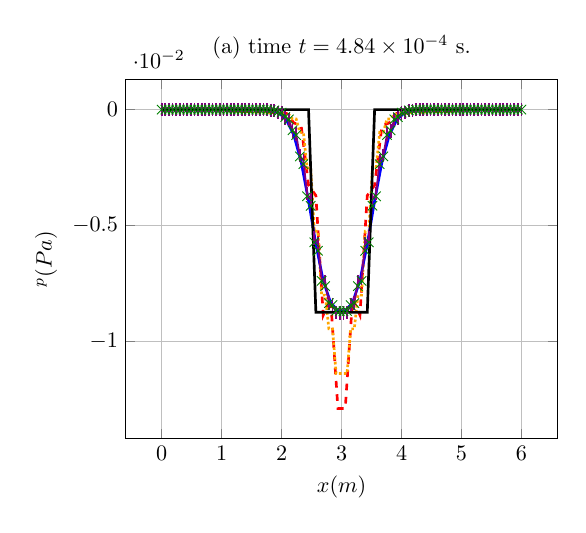
\begin{tikzpicture}[scale=0.8]
\begin{axis}[xlabel=$x (m)$,ylabel=$\eps^p (Pa)$,ymajorgrids=true,xmajorgrids=true,legend pos=outer north east,title={(a) time $t = 4.84\times 10^{-4} $ s.}]
\addplot[Red,very thick,mark=none,dashed,mark size=3pt] coordinates {(0.0,0.0) (0.12244897959183673,0.0) (0.24489795918367346,0.0) (0.36734693877551017,0.0) (0.4897959183673469,0.0) (0.6122448979591837,0.0) (0.7346938775510203,0.0) (0.8571428571428571,0.0) (0.9795918367346939,0.0) (1.1020408163265305,-3.791590211516079e-05) (1.2244897959183674,-7.70866275263142e-05) (1.346938775510204,-8.497586707829323e-05) (1.4693877551020407,-9.030872437715389e-05) (1.5918367346938775,-9.742060457186303e-05) (1.7142857142857142,-0.00011777294632526181) (1.836734693877551,-0.00011877997120884317) (1.9591836734693877,-0.00017229593911894644) (2.0816326530612246,-0.0001625095927714705) (2.204081632653061,-0.0005721718460187986) (2.326530612244898,-0.0006980928227095806) (2.4489795918367347,-0.003255684770391246) (2.571428571428571,-0.003703854150331533) (2.693877551020408,-0.008855536230217072) (2.816326530612245,-0.008134161982050364) (2.9387755102040813,-0.012877303196726952) (3.061224489795918,-0.012877303196726607) (3.183673469387755,-0.008134161982050527) (3.306122448979592,-0.008855536230216924) (3.4285714285714284,-0.00370385415033155) (3.5510204081632653,-0.0032556847703911866) (3.673469387755102,-0.0006980928227095723) (3.7959183673469385,-0.0005721718460187898) (3.9183673469387754,-0.0001625095927714674) (4.040816326530612,-0.00017229593911894956) (4.163265306122449,-0.00011877997120884148) (4.285714285714286,-0.00011777294632525957) (4.408163265306122,-9.74206045718636e-05) (4.530612244897959,-9.030872437715303e-05) (4.653061224489796,-8.497586707829776e-05) (4.775510204081632,-7.708662752631704e-05) (4.8979591836734695,-3.791590211516108e-05) (5.020408163265306,0.0) (5.142857142857142,0.0) (5.26530612244898,0.0) (5.387755102040816,0.0) (5.5102040816326525,0.0) (5.63265306122449,0.0) (5.755102040816326,0.0) (5.877551020408163,0.0) (6.0,0.0) };
\addplot[Orange,very thick,mark=none,densely dotted,mark size=3pt] coordinates {(0.0,0.0) (0.06060606060606061,0.0) (0.12121212121212122,0.0) (0.18181818181818182,0.0) (0.24242424242424243,0.0) (0.30303030303030304,0.0) (0.36363636363636365,0.0) (0.42424242424242425,0.0) (0.48484848484848486,0.0) (0.5454545454545454,0.0) (0.6060606060606061,0.0) (0.6666666666666667,0.0) (0.7272727272727273,0.0) (0.7878787878787878,0.0) (0.8484848484848485,0.0) (0.9090909090909092,0.0) (0.9696969696969697,0.0) (1.0303030303030303,0.0) (1.0909090909090908,-5.189503403045677e-05) (1.1515151515151516,-5.189503403045677e-05) (1.2121212121212122,-7.644801267914517e-05) (1.2727272727272727,-7.644801267914517e-05) (1.3333333333333335,-8.355081233240621e-05) (1.393939393939394,-8.355081233240621e-05) (1.4545454545454546,-8.910062882111044e-05) (1.5151515151515151,-8.910062882111044e-05) (1.5757575757575757,-9.397621508219469e-05) (1.6363636363636365,-9.397621508219469e-05) (1.696969696969697,-0.00010493025008663676) (1.7575757575757576,-0.00010493025008663676) (1.8181818181818183,-0.0001273466612942605) (1.878787878787879,-0.0001273466612942605) (1.9393939393939394,-0.00015215160027546855) (2.0,-0.00015215160027546855) (2.0606060606060606,-0.00020922085638282924) (2.121212121212121,-0.00020922085638282924) (2.1818181818181817,-0.00040275193843327815) (2.2424242424242427,-0.00040275193843327815) (2.303030303030303,-0.0009750544233862026) (2.3636363636363638,-0.0009750544233862026) (2.4242424242424243,-0.0025145499736588055) (2.484848484848485,-0.0025145499736588055) (2.5454545454545454,-0.005244570914165349) (2.606060606060606,-0.005244570914165349) (2.666666666666667,-0.007992615538684102) (2.7272727272727275,-0.007992615538684102) (2.787878787878788,-0.009446048408812087) (2.8484848484848486,-0.009446048408812087) (2.909090909090909,-0.011373543353957122) (2.9696969696969697,-0.011373543353957122) (3.0303030303030303,-0.011373543353957112) (3.090909090909091,-0.011373543353957112) (3.1515151515151514,-0.009446048408812087) (3.2121212121212124,-0.009446048408812087) (3.272727272727273,-0.007992615538684114) (3.3333333333333335,-0.007992615538684114) (3.393939393939394,-0.00524457091416535) (3.4545454545454546,-0.00524457091416535) (3.515151515151515,-0.002514549973658797) (3.5757575757575757,-0.002514549973658797) (3.6363636363636367,-0.0009750544233862052) (3.6969696969696972,-0.0009750544233862052) (3.757575757575758,-0.0004027519384332821) (3.8181818181818183,-0.0004027519384332821) (3.878787878787879,-0.00020922085638282406) (3.9393939393939394,-0.00020922085638282406) (4.0,-0.00015215160027546624) (4.0606060606060606,-0.00015215160027546624) (4.121212121212121,-0.0001273466612942568) (4.181818181818182,-0.0001273466612942568) (4.242424242424242,-0.0001049302500866464) (4.303030303030303,-0.0001049302500866464) (4.363636363636363,-9.397621508218874e-05) (4.424242424242425,-9.397621508218874e-05) (4.484848484848485,-8.910062882111044e-05) (4.545454545454546,-8.910062882111044e-05) (4.606060606060606,-8.35508123324031e-05) (4.666666666666667,-8.35508123324031e-05) (4.7272727272727275,-7.644801267914545e-05) (4.787878787878788,-7.644801267914545e-05) (4.848484848484849,-5.189503403045904e-05) (4.909090909090909,-5.189503403045904e-05) (4.96969696969697,0.0) (5.03030303030303,0.0) (5.090909090909091,0.0) (5.151515151515151,0.0) (5.212121212121212,0.0) (5.2727272727272725,0.0) (5.333333333333334,0.0) (5.3939393939393945,0.0) (5.454545454545455,0.0) (5.515151515151516,0.0) (5.575757575757576,0.0) (5.636363636363637,0.0) (5.696969696969697,0.0) (5.757575757575758,0.0) (5.818181818181818,0.0) (5.878787878787879,0.0) (5.9393939393939394,0.0) (6.0,0.0) };
\addplot[Blue,very thick,mark=none,solid,mark size=3pt] coordinates {(0.0,0.0) (0.12244897959183673,0.0) (0.24489795918367346,0.0) (0.36734693877551017,0.0) (0.4897959183673469,0.0) (0.6122448979591837,-5.222502208891369e-16) (0.7346938775510203,-3.801924841744559e-14) (0.8571428571428571,-1.3141666139875138e-12) (0.9795918367346939,-2.8745591924304055e-11) (1.1020408163265305,-4.464150179000128e-10) (1.2244897959183674,-5.23467841943105e-09) (1.346938775510204,-4.812046858639944e-08) (1.4693877551020407,-3.554036475964955e-07) (1.5918367346938775,-2.1443096765697003e-06) (1.7142857142857142,-1.0689498023182154e-05) (1.836734693877551,-4.436466051051049e-05) (1.9591836734693877,-0.00015404085928397946) (2.0816326530612246,-0.00044873332231471766) (2.204081632653061,-0.0010984305872627827) (2.326530612244898,-0.0022622254025038953) (2.4489795918367347,-0.003929978610103271) (2.571428571428571,-0.005797119893456445) (2.693877551020408,-0.007371043418348148) (2.816326530612245,-0.008310826779347521) (2.9387755102040813,-0.00866523151909913) (3.061224489795918,-0.008665231519099129) (3.183673469387755,-0.008310826779347523) (3.306122448979592,-0.007371043418348151) (3.4285714285714284,-0.0057971198934564485) (3.5510204081632653,-0.003929978610103277) (3.673469387755102,-0.002262225402503906) (3.7959183673469385,-0.0010984305872627934) (3.9183673469387754,-0.0004487333223147267) (4.040816326530612,-0.00015404085928398656) (4.163265306122449,-4.4364660510512195e-05) (4.285714285714286,-1.0689498023171936e-05) (4.408163265306122,-2.144309676557212e-06) (4.530612244897959,-3.554036475865614e-07) (4.653061224489796,-4.8120468574194675e-08) (4.775510204081632,-5.234678408361617e-09) (4.8979591836734695,-4.4641501165571666e-10) (5.020408163265306,-2.874559277579898e-11) (5.142857142857142,-1.314168884640648e-12) (5.26530612244898,-3.802009991237095e-14) (5.387755102040816,-5.242370423816499e-16) (5.5102040816326525,0.0) (5.63265306122449,0.0) (5.755102040816326,0.0) (5.877551020408163,0.0) (6.0,0.0) };
\addplot[Purple,thick,mark=|,solid,mark size=3pt] coordinates {(0.0,0.0) (0.06060606060606061,0.0) (0.12121212121212122,0.0) (0.18181818181818182,0.0) (0.24242424242424243,0.0) (0.30303030303030304,0.0) (0.36363636363636365,0.0) (0.42424242424242425,0.0) (0.48484848484848486,0.0) (0.5454545454545454,0.0) (0.6060606060606061,0.0) (0.6666666666666667,0.0) (0.7272727272727273,0.0) (0.7878787878787878,0.0) (0.8484848484848485,0.0) (0.9090909090909092,0.0) (0.9696969696969697,0.0) (1.0303030303030303,0.0) (1.0909090909090908,0.0) (1.1515151515151516,0.0) (1.2121212121212122,0.0) (1.2727272727272727,0.0) (1.3333333333333335,0.0) (1.393939393939394,-1.0241627792999857e-07) (1.4545454545454546,-2.1818139095136096e-07) (1.5151515151515151,-3.4092713152879763e-07) (1.5757575757575757,-1.326095171369825e-06) (1.6363636363636365,-1.9327126010610944e-06) (1.696969696969697,-7.1982977992651005e-06) (1.7575757575757576,-9.874516857163679e-06) (1.8181818181818183,-3.1832173941879044e-05) (1.878787878787879,-4.148900391485663e-05) (1.9393939393939394,-0.00011652978508307877) (2.0,-0.00014507560252168775) (2.0606060606060606,-0.00035655457656559516) (2.121212121212121,-0.00042570629865757397) (2.1818181818181817,-0.0009162020126129757) (2.2424242424242427,-0.00105240338850247) (2.303030303030303,-0.001980220164065959) (2.3636363636363638,-0.00219491468716409) (2.4242424242424243,-0.0036028496584267246) (2.484848484848485,-0.0038667957458958825) (2.5454545454545454,-0.005536333244818787) (2.606060606060606,-0.005779106783972591) (2.666666666666667,-0.007262784738374422) (2.7272727272727275,-0.007418212916281399) (2.787878787878788,-0.008338349466527659) (2.8484848484848486,-0.008398061506685966) (2.909090909090909,-0.00874932105310645) (2.9696969696969697,-0.00875906579314888) (3.0303030303030303,-0.008759065793148885) (3.090909090909091,-0.008749321053106454) (3.1515151515151514,-0.008398061506685973) (3.2121212121212124,-0.008338349466527662) (3.272727272727273,-0.007418212916281403) (3.3333333333333335,-0.007262784738374426) (3.393939393939394,-0.005779106783972596) (3.4545454545454546,-0.00553633324481879) (3.515151515151515,-0.0038667957458958873) (3.5757575757575757,-0.003602849658426731) (3.6363636363636367,-0.0021949146871640965) (3.6969696969696972,-0.0019802201640659674) (3.757575757575758,-0.0010524033885024758) (3.8181818181818183,-0.0009162020126129829) (3.878787878787879,-0.0004257062986575768) (3.9393939393939394,-0.0003565545765655975) (4.0,-0.00014507560252168976) (4.0606060606060606,-0.00011652978508308132) (4.121212121212121,-4.148900391485918e-05) (4.181818181818182,-3.183217394188217e-05) (4.242424242424242,-9.874516857165381e-06) (4.303030303030303,-7.198297799266805e-06) (4.363636363636363,-1.9327126010608106e-06) (4.424242424242425,-1.3260951713706767e-06) (4.484848484848485,-3.409271315302168e-07) (4.545454545454546,-2.181813909527801e-07) (4.606060606060606,-1.0241627793085007e-07) (4.666666666666667,0.0) (4.7272727272727275,0.0) (4.787878787878788,0.0) (4.848484848484849,0.0) (4.909090909090909,0.0) (4.96969696969697,0.0) (5.03030303030303,0.0) (5.090909090909091,0.0) (5.151515151515151,0.0) (5.212121212121212,0.0) (5.2727272727272725,0.0) (5.333333333333334,0.0) (5.3939393939393945,0.0) (5.454545454545455,0.0) (5.515151515151516,0.0) (5.575757575757576,0.0) (5.636363636363637,0.0) (5.696969696969697,0.0) (5.757575757575758,0.0) (5.818181818181818,0.0) (5.878787878787879,0.0) (5.9393939393939394,0.0) (6.0,0.0) };
\addplot[Green,thin,mark=x,only marks,mark size=3pt] coordinates {(0.0,0.0) (0.06060606060606061,0.0) (0.12121212121212122,0.0) (0.18181818181818182,0.0) (0.24242424242424243,0.0) (0.30303030303030304,0.0) (0.36363636363636365,0.0) (0.42424242424242425,0.0) (0.48484848484848486,0.0) (0.5454545454545454,0.0) (0.6060606060606061,-1.0501770746140254e-17) (0.6666666666666667,-2.639634268624442e-17) (0.7272727272727273,-1.3930456978934152e-15) (0.7878787878787878,-3.0883720942905973e-15) (0.8484848484848485,-7.001587322780064e-14) (0.9090909090909092,-1.4903431846981957e-13) (0.9696969696969697,-2.1913525604066395e-12) (1.0303030303030303,-4.464930579775855e-12) (1.0909090909090908,-4.77809454713549e-11) (1.1515151515151516,-9.306204035168602e-11) (1.2121212121212122,-7.711520115534465e-10) (1.2727272727272727,-1.4337170623597643e-09) (1.3333333333333335,-9.554857790753955e-09) (1.393939393939394,-1.693314060852641e-08) (1.4545454545454546,-9.304669079212916e-08) (1.5151515151515151,-1.5696122348791076e-07) (1.5757575757575757,-7.232737795415378e-07) (1.6363636363636365,-1.1597909965574741e-06) (1.696969696969697,-4.533752320027351e-06) (1.7575757575757576,-6.901910053169727e-06) (1.8181818181818183,-2.3065619941253325e-05) (1.878787878787879,-3.3299321505525566e-05) (1.9393939393939394,-9.55956969570753e-05) (2.0,-0.00013077312616477553) (2.0606060606060606,-0.0003233382771117707) (2.121212121212121,-0.000418991275671649) (2.1818181818181817,-0.000893176596649358) (2.2424242424242427,-0.001096836586440369) (2.303030303030303,-0.0020167583506237943) (2.3636363636363638,-0.0023508767096016648) (2.4242424242424243,-0.003733526786569201) (2.484848484848485,-0.004145706810179733) (2.5454545454545454,-0.005716170295994451) (2.606060606060606,-0.0060844115721184165) (2.666666666666667,-0.007382239901136897) (2.7272727272727275,-0.007606232648853957) (2.787878787878788,-0.008339693841572507) (2.8484848484848486,-0.00842236558917303) (2.909090909090909,-0.008674950007510287) (2.9696969696969697,-0.008688869601046518) (3.0303030303030303,-0.008688869601046518) (3.090909090909091,-0.008674950007510288) (3.1515151515151514,-0.008422365589173027) (3.2121212121212124,-0.008339693841572503) (3.272727272727273,-0.007606232648853953) (3.3333333333333335,-0.0073822399011368965) (3.393939393939394,-0.006084411572118416) (3.4545454545454546,-0.0057161702959944525) (3.515151515151515,-0.004145706810179732) (3.5757575757575757,-0.0037335267865692026) (3.6363636363636367,-0.0023508767096016643) (3.6969696969696972,-0.0020167583506237956) (3.757575757575758,-0.0010968365864403716) (3.8181818181818183,-0.0008931765966493632) (3.878787878787879,-0.0004189912756716515) (3.9393939393939394,-0.0003233382771117741) (4.0,-0.0001307731261647775) (4.0606060606060606,-9.559569695707617e-05) (4.121212121212121,-3.329932150552386e-05) (4.181818181818182,-2.3065619941252752e-05) (4.242424242424242,-6.901910053168876e-06) (4.303030303030303,-4.533752320026216e-06) (4.363636363636363,-1.15979099656088e-06) (4.424242424242425,-7.232737795452277e-07) (4.484848484848485,-1.5696122349358742e-07) (4.545454545454546,-9.304669079865728e-08) (4.606060606060606,-1.6933140614486876e-08) (4.666666666666667,-9.554857795862925e-09) (4.7272727272727275,-1.433717062643596e-09) (4.787878787878788,-7.711520118372781e-10) (4.848484848484849,-9.30620395001911e-11) (4.909090909090909,-4.778094547135489e-11) (4.96969696969697,-4.464928876786005e-12) (5.03030303030303,-2.191354547228132e-12) (5.090909090909091,-1.4903885977608817e-13) (5.151515151515151,-7.002013070242745e-14) (5.212121212121212,-3.0886559259323846e-15) (5.2727272727272725,-1.3902073814755395e-15) (5.333333333333334,-2.923465910412016e-17) (5.3939393939393945,-1.7313730149042037e-17) (5.454545454545455,0.0) (5.515151515151516,0.0) (5.575757575757576,0.0) (5.636363636363637,0.0) (5.696969696969697,0.0) (5.757575757575758,0.0) (5.818181818181818,0.0) (5.878787878787879,0.0) (5.9393939393939394,0.0) (6.0,0.0) };
\addplot[black,very thick,mark=pentagone*,solid,mark size=3pt] coordinates {(0.0,-0.0) (0.12244897959183673,-0.0) (0.24489795918367346,-0.0) (0.36734693877551017,-0.0) (0.4897959183673469,-0.0) (0.6122448979591837,-0.0) (0.7346938775510203,-0.0) (0.8571428571428571,-0.0) (0.9795918367346939,-0.0) (1.1020408163265305,-0.0) (1.2244897959183674,-0.0) (1.346938775510204,-0.0) (1.4693877551020407,-0.0) (1.5918367346938775,-0.0) (1.7142857142857142,-0.0) (1.836734693877551,-0.0) (1.9591836734693877,-0.0) (2.0816326530612246,-0.0) (2.204081632653061,-0.0) (2.326530612244898,-0.0) (2.4489795918367347,-0.0) (2.571428571428571,-0.008728715609439695) (2.693877551020408,-0.008728715609439695) (2.816326530612245,-0.008728715609439695) (2.9387755102040813,-0.008728715609439695) (3.061224489795918,-0.008728715609439695) (3.183673469387755,-0.008728715609439695) (3.306122448979592,-0.008728715609439695) (3.4285714285714284,-0.008728715609439695) (3.5510204081632653,-0.0) (3.673469387755102,-0.0) (3.7959183673469385,-0.0) (3.9183673469387754,-0.0) (4.040816326530612,-0.0) (4.163265306122449,-0.0) (4.285714285714286,-0.0) (4.408163265306122,-0.0) (4.530612244897959,-0.0) (4.653061224489796,-0.0) (4.775510204081632,-0.0) (4.8979591836734695,-0.0) (5.020408163265306,-0.0) (5.142857142857142,-0.0) (5.26530612244898,-0.0) (5.387755102040816,-0.0) (5.5102040816326525,-0.0) (5.63265306122449,-0.0) (5.755102040816326,-0.0) (5.877551020408163,-0.0) (6.0,-0.0) };
%\legend{usl 1ppc,usl 2ppc,dgmpm 1ppc,dgmpm 2ppc,dgmpm 2ppc (RK2),exact}
\end{axis}
\end{tikzpicture}
%%% Local Variables:
%%% mode: latex
%%% TeX-master: "../../mainManuscript"
%%% End:
}
%   {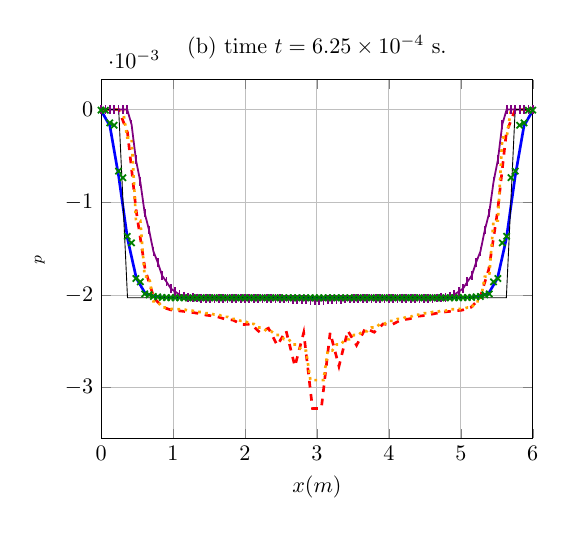
\begin{tikzpicture}[scale=0.8]
\begin{axis}[xlabel=$x (m)$,ylabel=$\eps^p$,ymajorgrids=true,xmajorgrids=true,legend pos=outer north east,title={(b) time $t = 6.25\times 10^{-4} $ s.},xmin=0.,xmax=6.]
\addplot[Red,very thick,mark=none,dashed] coordinates {(0.0,0.0) (0.12244897959183673,0.0) (0.24489795918367346,0.0) (0.36734693877551017,-0.0002478348228815541) (0.4897959183673469,-0.0011004378155012712) (0.6122448979591837,-0.0017260409269248597) (0.7346938775510203,-0.002031865332982762) (0.8571428571428571,-0.002132968518977378) (0.9795918367346939,-0.0021636018350532395) (1.1020408163265305,-0.0021733079916121177) (1.2244897959183674,-0.00218350748748031) (1.346938775510204,-0.002198645448466017) (1.4693877551020407,-0.002218920213241705) (1.5918367346938775,-0.002229697455331896) (1.7142857142857142,-0.002258121963594508) (1.836734693877551,-0.002271799079674154) (1.9591836734693877,-0.002320613632318322) (2.0816326530612246,-0.002313868472160546) (2.204081632653061,-0.0024020122032007017) (2.326530612244898,-0.0023588630990294623) (2.4489795918367347,-0.0025433455597807667) (2.571428571428571,-0.002385435935351422) (2.693877551020408,-0.0027693350417516906) (2.816326530612245,-0.0024065265204776445) (2.9387755102040813,-0.0032250612006492966) (3.061224489795918,-0.0032250612006492524) (3.183673469387755,-0.002406526520477666) (3.306122448979592,-0.0027693350417516823) (3.4285714285714284,-0.0023854359353514295) (3.5510204081632653,-0.0025433455597807628) (3.673469387755102,-0.002358863099029464) (3.7959183673469385,-0.0024020122032006983) (3.9183673469387754,-0.0023138684721605448) (4.040816326530612,-0.002320613632318319) (4.163265306122449,-0.0022717990796741546) (4.285714285714286,-0.0022581219635945077) (4.408163265306122,-0.0022296974553318956) (4.530612244897959,-0.0022189202132417056) (4.653061224489796,-0.0021986454484660173) (4.775510204081632,-0.0021835074874803095) (4.8979591836734695,-0.0021733079916121186) (5.020408163265306,-0.0021636018350532395) (5.142857142857142,-0.002132968518977378) (5.26530612244898,-0.002031865332982763) (5.387755102040816,-0.0017260409269248577) (5.5102040816326525,-0.0011004378155012658) (5.63265306122449,-0.0002478348228815494) (5.755102040816326,0.0) (5.877551020408163,0.0) (6.0,0.0) };
\addplot[Orange,very thick,mark=none,dotted] coordinates {(0.0,0.0) (0.06060606060606061,0.0) (0.12121212121212122,0.0) (0.18181818181818182,0.0) (0.24242424242424243,0.0) (0.30303030303030304,0.0) (0.36363636363636365,-0.0003017574960527518) (0.42424242424242425,-0.0003017574960527518) (0.48484848484848486,-0.0011974917980669022) (0.5454545454545454,-0.0011974917980669022) (0.6060606060606061,-0.0018020040797071544) (0.6666666666666667,-0.0018020040797071544) (0.7272727272727273,-0.002068378033006087) (0.7878787878787878,-0.002068378033006087) (0.8484848484848485,-0.002135941628228986) (0.9090909090909092,-0.002135941628228986) (0.9696969696969697,-0.002150822172714686) (1.0303030303030303,-0.002150822172714686) (1.0909090909090908,-0.002154888242838099) (1.1515151515151516,-0.002154888242838099) (1.2121212121212122,-0.0021700900543690626) (1.2727272727272727,-0.0021700900543690626) (1.3333333333333335,-0.0021843706812353886) (1.393939393939394,-0.0021843706812353886) (1.4545454545454546,-0.0021968313010739355) (1.5151515151515151,-0.0021968313010739355) (1.5757575757575757,-0.0022123334205993417) (1.6363636363636365,-0.0022123334205993417) (1.696969696969697,-0.0022365941606657474) (1.7575757575757576,-0.0022365941606657474) (1.8181818181818183,-0.0022585940891309796) (1.878787878787879,-0.0022585940891309796) (1.9393939393939394,-0.0022798424574663194) (2.0,-0.0022798424574663194) (2.0606060606060606,-0.0023117041253564387) (2.121212121212121,-0.0023117041253564387) (2.1818181818181817,-0.002350782112768782) (2.2424242424242427,-0.002350782112768782) (2.303030303030303,-0.002390940396871615) (2.3636363636363638,-0.002390940396871615) (2.4242424242424243,-0.0024313395034050904) (2.484848484848485,-0.0024313395034050904) (2.5454545454545454,-0.002477563584428502) (2.606060606060606,-0.002477563584428502) (2.666666666666667,-0.0025344573000873694) (2.7272727272727275,-0.0025344573000873694) (2.787878787878788,-0.002600834768573611) (2.8484848484848486,-0.002600834768573611) (2.909090909090909,-0.0029191565184019295) (2.9696969696969697,-0.0029191565184019295) (3.0303030303030303,-0.0029191565184019273) (3.090909090909091,-0.0029191565184019273) (3.1515151515151514,-0.0026008347685736143) (3.2121212121212124,-0.0026008347685736143) (3.272727272727273,-0.002534457300087371) (3.3333333333333335,-0.002534457300087371) (3.393939393939394,-0.0024775635844285025) (3.4545454545454546,-0.0024775635844285025) (3.515151515151515,-0.0024313395034050896) (3.5757575757575757,-0.0024313395034050896) (3.6363636363636367,-0.002390940396871615) (3.6969696969696972,-0.002390940396871615) (3.757575757575758,-0.0023507821127687826) (3.8181818181818183,-0.0023507821127687826) (3.878787878787879,-0.002311704125356438) (3.9393939393939394,-0.002311704125356438) (4.0,-0.0022798424574663172) (4.0606060606060606,-0.0022798424574663172) (4.121212121212121,-0.00225859408913098) (4.181818181818182,-0.00225859408913098) (4.242424242424242,-0.002236594160665746) (4.303030303030303,-0.002236594160665746) (4.363636363636363,-0.0022123334205993426) (4.424242424242425,-0.0022123334205993426) (4.484848484848485,-0.002196831301073935) (4.545454545454546,-0.002196831301073935) (4.606060606060606,-0.0021843706812353886) (4.666666666666667,-0.0021843706812353886) (4.7272727272727275,-0.0021700900543690613) (4.787878787878788,-0.0021700900543690613) (4.848484848484849,-0.0021548882428381) (4.909090909090909,-0.0021548882428381) (4.96969696969697,-0.0021508221727146843) (5.03030303030303,-0.0021508221727146843) (5.090909090909091,-0.002135941628228984) (5.151515151515151,-0.002135941628228984) (5.212121212121212,-0.0020683780330060866) (5.2727272727272725,-0.0020683780330060866) (5.333333333333334,-0.0018020040797071535) (5.3939393939393945,-0.0018020040797071535) (5.454545454545455,-0.0011974917980669003) (5.515151515151516,-0.0011974917980669003) (5.575757575757576,-0.0003017574960527513) (5.636363636363637,-0.0003017574960527513) (5.696969696969697,0.0) (5.757575757575758,0.0) (5.818181818181818,0.0) (5.878787878787879,0.0) (5.9393939393939394,0.0) (6.0,0.0) };
\addplot[Blue,very thick,mark=none,solid] coordinates {(0.0,-8.02367288935203e-06) (0.12244897959183673,-0.00017614426387335805) (0.24489795918367346,-0.0007207542691858686) (0.36734693877551017,-0.0013919930410856215) (0.4897959183673469,-0.001818355598439618) (0.6122448979591837,-0.001981300761387861) (0.7346938775510203,-0.0020125975551096974) (0.8571428571428571,-0.002024874952136019) (0.9795918367346939,-0.0020290867696967987) (1.1020408163265305,-0.002030353909504423) (1.2244897959183674,-0.0020306887880741907) (1.346938775510204,-0.0020307665725143873) (1.4693877551020407,-0.0020307824435747243) (1.5918367346938775,-0.0020307852835259937) (1.7142857142857142,-0.0020307857279245408) (1.836734693877551,-0.0020307857884822454) (1.9591836734693877,-0.00203078579562695) (2.0816326530612246,-0.002030785796351117) (2.204081632653061,-0.0020307857964135248) (2.326530612244898,-0.002030785796418031) (2.4489795918367347,-0.002030785796418302) (2.571428571428571,-0.0020307857964183135) (2.693877551020408,-0.002030785796418313) (2.816326530612245,-0.002030785796418313) (2.9387755102040813,-0.002030785796418314) (3.061224489795918,-0.0020307857964183135) (3.183673469387755,-0.0020307857964183135) (3.306122448979592,-0.0020307857964183126) (3.4285714285714284,-0.0020307857964183113) (3.5510204081632653,-0.0020307857964183005) (3.673469387755102,-0.002030785796418031) (3.7959183673469385,-0.0020307857964135217) (3.9183673469387754,-0.0020307857963511138) (4.040816326530612,-0.002030785795626948) (4.163265306122449,-0.0020307857884822433) (4.285714285714286,-0.0020307857279245403) (4.408163265306122,-0.0020307852835259915) (4.530612244897959,-0.0020307824435747226) (4.653061224489796,-0.0020307665725143842) (4.775510204081632,-0.002030688788074188) (4.8979591836734695,-0.0020303539095044196) (5.020408163265306,-0.0020290867696967953) (5.142857142857142,-0.0020248749521360144) (5.26530612244898,-0.0020125975551096966) (5.387755102040816,-0.0019813007613878565) (5.5102040816326525,-0.0018183555984396154) (5.63265306122449,-0.0013919930410856195) (5.755102040816326,-0.0007207542691858678) (5.877551020408163,-0.0001761442638733595) (6.0,-8.023672889353243e-06) };
\addplot[Purple,thick,mark=|,solid] coordinates {(0.0,0.0) (0.06060606060606061,0.0) (0.12121212121212122,0.0) (0.18181818181818182,0.0) (0.24242424242424243,0.0) (0.30303030303030304,0.0) (0.36363636363636365,0.0) (0.42424242424242425,-0.00016170662401525856) (0.48484848484848486,-0.0005417551163059964) (0.5454545454545454,-0.0007797468469340016) (0.6060606060606061,-0.0011158014314235371) (0.6666666666666667,-0.0012988809897543044) (0.7272727272727273,-0.0015295338295444575) (0.7878787878787878,-0.0016494591967999013) (0.8484848484848485,-0.001791241808636007) (0.9090909090909092,-0.001858139654558482) (0.9696969696969697,-0.0019313228858157505) (1.0303030303030303,-0.001963941276484258) (1.0909090909090908,-0.00199709045414516) (1.1515151515151516,-0.0020110149368315873) (1.2121212121212122,-0.0020240838020015965) (1.2727272727272727,-0.002029112099138213) (1.3333333333333335,-0.002033444493020763) (1.393939393939394,-0.0020349375209240046) (1.4545454545454546,-0.0020360626617364976) (1.5151515151515151,-0.002036427946256999) (1.5757575757575757,-0.0020366368397527423) (1.6363636363636365,-0.002036698090585699) (1.696969696969697,-0.0020368405580576125) (1.7575757575757576,-0.0020369810286138333) (1.8181818181818183,-0.0020373219984231514) (1.878787878787879,-0.002037585653215558) (1.9393939393939394,-0.002037962720224221) (2.0,-0.002038127417033818) (2.0606060606060606,-0.0020383611759408468) (2.121212121212121,-0.002038518677096413) (2.1818181818181817,-0.0020388624173375575) (2.2424242424242427,-0.002039197521601926) (2.303030303030303,-0.0020400227446406255) (2.3636363636363638,-0.0020406530704546125) (2.4242424242424243,-0.0020416018700111314) (2.484848484848485,-0.00204214484166886) (2.5454545454545454,-0.002043028167195094) (2.606060606060606,-0.0020436145435565973) (2.666666666666667,-0.0020449363268448036) (2.7272727272727275,-0.0020459859423928813) (2.787878787878788,-0.002048543419164452) (2.8484848484848486,-0.002051015793534283) (2.909090909090909,-0.0020569476212071243) (2.9696969696969697,-0.0020621904992435833) (3.0303030303030303,-0.0020621904992435824) (3.090909090909091,-0.002056947621207125) (3.1515151515151514,-0.0020510157935342823) (3.2121212121212124,-0.002048543419164453) (3.272727272727273,-0.0020459859423928826) (3.3333333333333335,-0.0020449363268448045) (3.393939393939394,-0.0020436145435565965) (3.4545454545454546,-0.002043028167195095) (3.515151515151515,-0.0020421448416688593) (3.5757575757575757,-0.002041601870011131) (3.6363636363636367,-0.00204065307045461) (3.6969696969696972,-0.0020400227446406246) (3.757575757575758,-0.0020391975216019266) (3.8181818181818183,-0.002038862417337557) (3.878787878787879,-0.002038518677096414) (3.9393939393939394,-0.0020383611759408476) (4.0,-0.002038127417033818) (4.0606060606060606,-0.002037962720224222) (4.121212121212121,-0.0020375856532155604) (4.181818181818182,-0.002037321998423153) (4.242424242424242,-0.002036981028613838) (4.303030303030303,-0.0020368405580576134) (4.363636363636363,-0.002036698090585699) (4.424242424242425,-0.0020366368397527414) (4.484848484848485,-0.002036427946257001) (4.545454545454546,-0.0020360626617365023) (4.606060606060606,-0.0020349375209240063) (4.666666666666667,-0.002033444493020765) (4.7272727272727275,-0.002029112099138214) (4.787878787878788,-0.0020240838020015987) (4.848484848484849,-0.00201101493683159) (4.909090909090909,-0.0019970904541451633) (4.96969696969697,-0.001963941276484259) (5.03030303030303,-0.0019313228858157542) (5.090909090909091,-0.0018581396545584844) (5.151515151515151,-0.0017912418086360104) (5.212121212121212,-0.001649459196799904) (5.2727272727272725,-0.001529533829544461) (5.333333333333334,-0.0012988809897543081) (5.3939393939393945,-0.0011158014314235415) (5.454545454545455,-0.000779746846934003) (5.515151515151516,-0.0005417551163059989) (5.575757575757576,-0.00016170662401526048) (5.636363636363637,0.0) (5.696969696969697,0.0) (5.757575757575758,0.0) (5.818181818181818,0.0) (5.878787878787879,0.0) (5.9393939393939394,0.0) (6.0,0.0) };
\addplot[Green,thick,mark=x,only marks] coordinates {(0.0,-5.335532070735344e-06) (0.06060606060606061,-6.7706518097916305e-06) (0.12121212121212122,-0.00014296272370405532) (0.18181818181818182,-0.00016863154669993438) (0.24242424242424243,-0.0006638300086644545) (0.30303030303030304,-0.000734378934081307) (0.36363636363636365,-0.0013668887954266346) (0.42424242424242425,-0.0014381987584863236) (0.48484848484848486,-0.0018228537169639558) (0.5454545454545454,-0.0018582326659348394) (0.6060606060606061,-0.0019882143939252963) (0.6666666666666667,-0.001998178050264291) (0.7272727272727273,-0.0020167573045254297) (0.7878787878787878,-0.0020205950613102187) (0.8484848484848485,-0.0020268204253525244) (0.9090909090909092,-0.0020280653889615647) (0.9696969696969697,-0.0020298272803462047) (1.0303030303030303,-0.002030167668233374) (1.0909090909090908,-0.0020305882754214715) (1.1515151515151516,-0.0020306665744077384) (1.2121212121212122,-0.002030751197289206) (1.2727272727272727,-0.002030766353237554) (1.3333333333333335,-0.0020307803579508853) (1.393939393939394,-0.002030782732084688) (1.4545454545454546,-0.002030784516510227) (1.5151515151515151,-0.0020307847942330386) (1.5757575757575757,-0.0020307855174271218) (1.6363636363636365,-0.0020307856825908114) (1.696969696969697,-0.002030785724102555) (1.7575757575757576,-0.0020307858759962597) (1.8181818181818183,-0.002030785951180978) (1.878787878787879,-0.0020307860418172555) (1.9393939393939394,-0.002030786134808208) (2.0,-0.002030786322147464) (2.0606060606060606,-0.0020307863445982147) (2.121212121212121,-0.0020307866728231407) (2.1818181818181817,-0.0020307867744393435) (2.2424242424242427,-0.002030787015486384) (2.303030303030303,-0.002030787409711756) (2.3636363636363638,-0.0020307883320914285) (2.4242424242424243,-0.0020307890300132712) (2.484848484848485,-0.0020307901307202374) (2.5454545454545454,-0.002030792281554236) (2.606060606060606,-0.002030795453324907) (2.666666666666667,-0.0020307979071881566) (2.7272727272727275,-0.0020308065650964362) (2.787878787878788,-0.002030816863285245) (2.8484848484848486,-0.0020308137021312345) (2.909090909090909,-0.0020308908094497746) (2.9696969696969697,-0.002031166801141057) (3.0303030303030303,-0.0020311668011410568) (3.090909090909091,-0.002030890809449775) (3.1515151515151514,-0.002030813702131235) (3.2121212121212124,-0.002030816863285247) (3.272727272727273,-0.002030806565096435) (3.3333333333333335,-0.0020307979071881553) (3.393939393939394,-0.0020307954533249043) (3.4545454545454546,-0.0020307922815542352) (3.515151515151515,-0.0020307901307202374) (3.5757575757575757,-0.0020307890300132712) (3.6363636363636367,-0.00203078833209143) (3.6969696969696972,-0.002030787409711759) (3.757575757575758,-0.0020307870154863874) (3.8181818181818183,-0.002030786774439345) (3.878787878787879,-0.0020307866728231446) (3.9393939393939394,-0.0020307863445982177) (4.0,-0.0020307863221474677) (4.0606060606060606,-0.002030786134808209) (4.121212121212121,-0.002030786041817254) (4.181818181818182,-0.0020307859511809767) (4.242424242424242,-0.0020307858759962614) (4.303030303030303,-0.002030785724102557) (4.363636363636363,-0.0020307856825908114) (4.424242424242425,-0.002030785517427123) (4.484848484848485,-0.00203078479423304) (4.545454545454546,-0.0020307845165102286) (4.606060606060606,-0.0020307827320846885) (4.666666666666667,-0.002030780357950887) (4.7272727272727275,-0.002030766353237556) (4.787878787878788,-0.0020307511972892083) (4.848484848484849,-0.00203066657440774) (4.909090909090909,-0.0020305882754214715) (4.96969696969697,-0.002030167668233377) (5.03030303030303,-0.002029827280346208) (5.090909090909091,-0.0020280653889615655) (5.151515151515151,-0.002026820425352526) (5.212121212121212,-0.002020595061310217) (5.2727272727272725,-0.0020167573045254293) (5.333333333333334,-0.001998178050264289) (5.3939393939393945,-0.001988214393925294) (5.454545454545455,-0.001858232665934836) (5.515151515151516,-0.0018228537169639517) (5.575757575757576,-0.0014381987584863212) (5.636363636363637,-0.0013668887954266316) (5.696969696969697,-0.0007343789340813044) (5.757575757575758,-0.0006638300086644511) (5.818181818181818,-0.00016863154669993243) (5.878787878787879,-0.0001429627237040512) (5.9393939393939394,-6.770651809786295e-06) (6.0,-5.335532070731949e-06) };
\addplot[black,thin,mark=none,solid] coordinates {(0.0,-0.0) (0.12244897959183673,-0.0) (0.24489795918367346,-0.0) (0.36734693877551017,-0.002030785796418313) (0.4897959183673469,-0.002030785796418313) (0.6122448979591837,-0.002030785796418313) (0.7346938775510203,-0.002030785796418313) (0.8571428571428571,-0.002030785796418313) (0.9795918367346939,-0.002030785796418313) (1.1020408163265305,-0.002030785796418313) (1.2244897959183674,-0.002030785796418313) (1.346938775510204,-0.002030785796418313) (1.4693877551020407,-0.002030785796418313) (1.5918367346938775,-0.002030785796418313) (1.7142857142857142,-0.002030785796418313) (1.836734693877551,-0.002030785796418313) (1.9591836734693877,-0.002030785796418313) (2.0816326530612246,-0.002030785796418313) (2.204081632653061,-0.002030785796418313) (2.326530612244898,-0.002030785796418313) (2.4489795918367347,-0.002030785796418313) (2.571428571428571,-0.002030785796418313) (2.693877551020408,-0.002030785796418313) (2.816326530612245,-0.002030785796418313) (2.9387755102040813,-0.002030785796418313) (3.061224489795918,-0.002030785796418313) (3.183673469387755,-0.002030785796418313) (3.306122448979592,-0.002030785796418313) (3.4285714285714284,-0.002030785796418313) (3.5510204081632653,-0.002030785796418313) (3.673469387755102,-0.002030785796418313) (3.7959183673469385,-0.002030785796418313) (3.9183673469387754,-0.002030785796418313) (4.040816326530612,-0.002030785796418313) (4.163265306122449,-0.002030785796418313) (4.285714285714286,-0.002030785796418313) (4.408163265306122,-0.002030785796418313) (4.530612244897959,-0.002030785796418313) (4.653061224489796,-0.002030785796418313) (4.775510204081632,-0.002030785796418313) (4.8979591836734695,-0.002030785796418313) (5.020408163265306,-0.002030785796418313) (5.142857142857142,-0.002030785796418313) (5.26530612244898,-0.002030785796418313) (5.387755102040816,-0.002030785796418313) (5.5102040816326525,-0.002030785796418313) (5.63265306122449,-0.002030785796418313) (5.755102040816326,-0.0) (5.877551020408163,-0.0) (6.0,-0.0) };
%\legend{usl 1ppc,usl 2ppc,dgmpm 1ppc,dgmpm 2ppc,dgmpm 2ppc (RK2),exact}
\end{axis}
\end{tikzpicture}
%%% Local Variables:
%%% mode: latex
%%% TeX-master: "../../mainManuscript"
%%% End:
}
%   {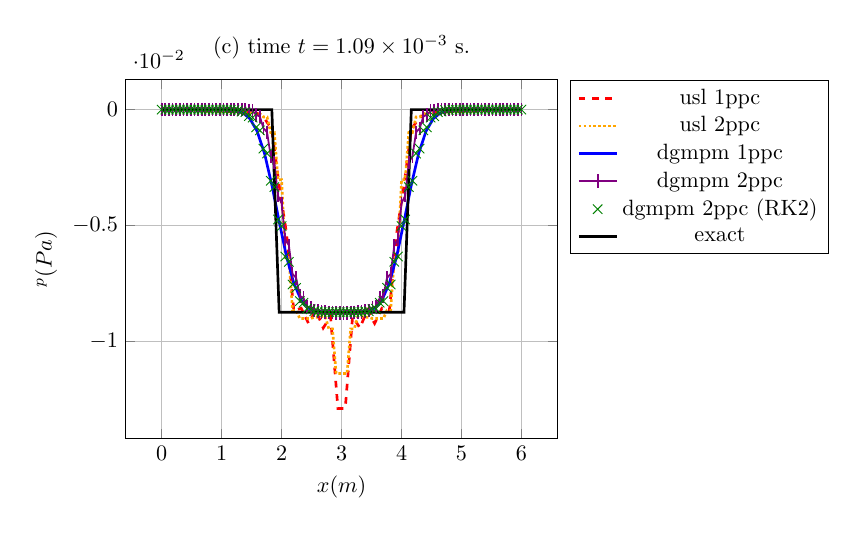
\begin{tikzpicture}[scale=0.8]
\begin{axis}[xlabel=$x (m)$,ylabel=$\eps^p (Pa)$,ymajorgrids=true,xmajorgrids=true,legend pos=outer north east,title={(c) time $t = 1.09\times 10^{-3} $ s.}]
\addplot[Red,very thick,mark=none,dashed,mark size=3pt] coordinates {(0.0,0.0) (0.12244897959183673,0.0) (0.24489795918367346,0.0) (0.36734693877551017,0.0) (0.4897959183673469,0.0) (0.6122448979591837,-3.577487902203997e-05) (0.7346938775510203,-6.306588245633642e-05) (0.8571428571428571,-6.949496312549484e-05) (0.9795918367346939,-8.005219978840035e-05) (1.1020408163265305,-9.009475914811774e-05) (1.2244897959183674,-9.858795071160678e-05) (1.346938775510204,-0.00010648019894997112) (1.4693877551020407,-0.00013090237763271645) (1.5918367346938775,-0.00015585484694440393) (1.7142857142857142,-0.00037807434010367157) (1.836734693877551,-0.0008542508721889013) (1.9591836734693877,-0.003265580636192999) (2.0816326530612246,-0.005332403663610279) (2.204081632653061,-0.008685547798871193) (2.326530612244898,-0.008557827562005196) (2.4489795918367347,-0.009212270529983918) (2.571428571428571,-0.008640321746270047) (2.693877551020408,-0.009408157524816411) (2.816326530612245,-0.008914806029937274) (2.9387755102040813,-0.012877303196726952) (3.061224489795918,-0.012877303196726607) (3.183673469387755,-0.008914806029937388) (3.306122448979592,-0.00940815752481628) (3.4285714285714284,-0.008640321746270135) (3.5510204081632653,-0.009212270529983827) (3.673469387755102,-0.008557827562005267) (3.7959183673469385,-0.008685547798871113) (3.9183673469387754,-0.005332403663610266) (4.040816326530612,-0.003265580636192934) (4.163265306122449,-0.0008542508721888987) (4.285714285714286,-0.00037807434010366447) (4.408163265306122,-0.00015585484694441217) (4.530612244897959,-0.00013090237763272187) (4.653061224489796,-0.00010648019894998299) (4.775510204081632,-9.858795071160708e-05) (4.8979591836734695,-9.00947591481104e-05) (5.020408163265306,-8.005219978840008e-05) (5.142857142857142,-6.949496312550109e-05) (5.26530612244898,-6.306588245633955e-05) (5.387755102040816,-3.5774879022040825e-05) (5.5102040816326525,0.0) (5.63265306122449,0.0) (5.755102040816326,0.0) (5.877551020408163,0.0) (6.0,0.0) };
\addplot[Orange,very thick,mark=none,densely dotted,mark size=3pt] coordinates {(0.0,0.0) (0.06060606060606061,0.0) (0.12121212121212122,0.0) (0.18181818181818182,0.0) (0.24242424242424243,0.0) (0.30303030303030304,0.0) (0.36363636363636365,0.0) (0.42424242424242425,0.0) (0.48484848484848486,-1.3923950014088835e-06) (0.5454545454545454,-1.3923950014088835e-06) (0.6060606060606061,-4.802593874190819e-05) (0.6666666666666667,-4.802593874190819e-05) (0.7272727272727273,-6.41910410194221e-05) (0.7878787878787878,-6.41910410194221e-05) (0.8484848484848485,-6.859024545017706e-05) (0.9090909090909092,-6.859024545017706e-05) (0.9696969696969697,-7.288774581652991e-05) (1.0303030303030303,-7.288774581652991e-05) (1.0909090909090908,-8.507726423586093e-05) (1.1515151515151516,-8.507726423586093e-05) (1.2121212121212122,-9.691077127878779e-05) (1.2727272727272727,-9.691077127878779e-05) (1.3333333333333335,-0.00010711649363712468) (1.393939393939394,-0.00010711649363712468) (1.4545454545454546,-0.00012487268940087668) (1.5151515151515151,-0.00012487268940087668) (1.5757575757575757,-0.00016846150368530778) (1.6363636363636365,-0.00016846150368530778) (1.696969696969697,-0.00032141238951341054) (1.7575757575757576,-0.00032141238951341054) (1.8181818181818183,-0.0009863835722303473) (1.878787878787879,-0.0009863835722303473) (1.9393939393939394,-0.003025063907376677) (2.0,-0.003025063907376677) (2.0606060606060606,-0.006366348809033719) (2.121212121212121,-0.006366348809033719) (2.1818181818181817,-0.008647239978151484) (2.2424242424242427,-0.008647239978151484) (2.303030303030303,-0.009001860585213824) (2.3636363636363638,-0.009001860585213824) (2.4242424242424243,-0.009001507335175213) (2.484848484848485,-0.009001507335175213) (2.5454545454545454,-0.008949274888554966) (2.606060606060606,-0.008949274888554966) (2.666666666666667,-0.00891581762874243) (2.7272727272727275,-0.00891581762874243) (2.787878787878788,-0.00944634271615033) (2.8484848484848486,-0.00944634271615033) (2.909090909090909,-0.011373543353957122) (2.9696969696969697,-0.011373543353957122) (3.0303030303030303,-0.011373543353957112) (3.090909090909091,-0.011373543353957112) (3.1515151515151514,-0.009446342716150326) (3.2121212121212124,-0.009446342716150326) (3.272727272727273,-0.00891581762874244) (3.3333333333333335,-0.00891581762874244) (3.393939393939394,-0.008949274888554966) (3.4545454545454546,-0.008949274888554966) (3.515151515151515,-0.009001507335175215) (3.5757575757575757,-0.009001507335175215) (3.6363636363636367,-0.009001860585213826) (3.6969696969696972,-0.009001860585213826) (3.757575757575758,-0.008647239978151493) (3.8181818181818183,-0.008647239978151493) (3.878787878787879,-0.006366348809033716) (3.9393939393939394,-0.006366348809033716) (4.0,-0.003025063907376669) (4.0606060606060606,-0.003025063907376669) (4.121212121212121,-0.0009863835722303564) (4.181818181818182,-0.0009863835722303564) (4.242424242424242,-0.00032141238951339976) (4.303030303030303,-0.00032141238951339976) (4.363636363636363,-0.00016846150368530894) (4.424242424242425,-0.00016846150368530894) (4.484848484848485,-0.00012487268940087758) (4.545454545454546,-0.00012487268940087758) (4.606060606060606,-0.00010711649363712272) (4.666666666666667,-0.00010711649363712272) (4.7272727272727275,-9.691077127878893e-05) (4.787878787878788,-9.691077127878893e-05) (4.848484848484849,-8.507726423586494e-05) (4.909090909090909,-8.507726423586494e-05) (4.96969696969697,-7.288774581652709e-05) (5.03030303030303,-7.288774581652709e-05) (5.090909090909091,-6.859024545017819e-05) (5.151515151515151,-6.859024545017819e-05) (5.212121212121212,-6.419104101942352e-05) (5.2727272727272725,-6.419104101942352e-05) (5.333333333333334,-4.8025938741907344e-05) (5.3939393939393945,-4.8025938741907344e-05) (5.454545454545455,-1.3923950014085998e-06) (5.515151515151516,-1.3923950014085998e-06) (5.575757575757576,0.0) (5.636363636363637,0.0) (5.696969696969697,0.0) (5.757575757575758,0.0) (5.818181818181818,0.0) (5.878787878787879,0.0) (5.9393939393939394,0.0) (6.0,0.0) };
\addplot[Blue,very thick,mark=none,solid,mark size=3pt] coordinates {(0.0,-5.676632835751488e-19) (0.12244897959183673,-2.3898624238513766e-16) (0.24489795918367346,-3.735990751357306e-14) (0.36734693877551017,-2.3089144911084856e-12) (0.4897959183673469,-7.596762237094698e-11) (0.6122448979591837,-1.5415975357804979e-09) (0.7346938775510203,-2.1087029002110162e-08) (0.8571428571428571,-2.0628580472526095e-07) (0.9795918367346939,-1.5051975779320511e-06) (1.1020408163265305,-8.452232526292688e-06) (1.2244897959183674,-3.741900938747327e-05) (1.346938775510204,-0.00013315210803806102) (1.4693877551020407,-0.00038701776930482674) (1.5918367346938775,-0.0009319386970470464) (1.7142857142857142,-0.0018842066770200564) (1.836734693877551,-0.0032431409441831516) (1.9591836734693877,-0.004827293901207316) (2.0816326530612246,-0.00633202118341673) (2.204081632653061,-0.007489880430691718) (2.326530612244898,-0.008204526972019307) (2.4489795918367347,-0.008552921390073501) (2.571428571428571,-0.008674876019514461) (2.693877551020408,-0.008716486656783273) (2.816326530612245,-0.008726887116624966) (2.9387755102040813,-0.008728580772745199) (3.061224489795918,-0.008728580772745199) (3.183673469387755,-0.008726887116624966) (3.306122448979592,-0.00871648665678328) (3.4285714285714284,-0.008674876019514466) (3.5510204081632653,-0.008552921390073511) (3.673469387755102,-0.008204526972019318) (3.7959183673469385,-0.007489880430691721) (3.9183673469387754,-0.00633202118341673) (4.040816326530612,-0.0048272939012073204) (4.163265306122449,-0.0032431409441831525) (4.285714285714286,-0.001884206677020053) (4.408163265306122,-0.0009319386970470392) (4.530612244897959,-0.0003870177693048181) (4.653061224489796,-0.0001331521080380519) (4.775510204081632,-3.7419009387462476e-05) (4.8979591836734695,-8.452232526284741e-06) (5.020408163265306,-1.5051975779246716e-06) (5.142857142857142,-2.0628580471617835e-07) (5.26530612244898,-2.1087028991608393e-08) (5.387755102040816,-1.5415975312391917e-09) (5.5102040816326525,-7.596762123562041e-11) (5.63265306122449,-2.308913923445202e-12) (5.755102040816326,-3.7358772187005907e-14) (5.877551020408163,-2.4097306387765065e-16) (6.0,-8.514949253627233e-19) };
\addplot[Purple,thick,mark=|,solid,mark size=3pt] coordinates {(0.0,0.0) (0.06060606060606061,0.0) (0.12121212121212122,0.0) (0.18181818181818182,0.0) (0.24242424242424243,0.0) (0.30303030303030304,0.0) (0.36363636363636365,0.0) (0.42424242424242425,0.0) (0.48484848484848486,0.0) (0.5454545454545454,0.0) (0.6060606060606061,0.0) (0.6666666666666667,0.0) (0.7272727272727273,0.0) (0.7878787878787878,0.0) (0.8484848484848485,0.0) (0.9090909090909092,0.0) (0.9696969696969697,0.0) (1.0303030303030303,0.0) (1.0909090909090908,0.0) (1.1515151515151516,-4.1375394533929374e-08) (1.2121212121212122,-1.6766275644359134e-07) (1.2727272727272727,-3.6899460485265364e-07) (1.3333333333333335,-3.7730684118324803e-06) (1.393939393939394,-6.566829345463855e-06) (1.4545454545454546,-3.9533489461271815e-05) (1.5151515151515151,-5.787873091723124e-05) (1.5757575757575757,-0.0002274525995650831) (1.6363636363636365,-0.00029636567097843057) (1.696969696969697,-0.0008043486101741406) (1.7575757575757576,-0.0009756904136278646) (1.8181818181818183,-0.002007506978689405) (1.878787878787879,-0.0022778320644552875) (1.9393939393939394,-0.0037101075201987303) (2.0,-0.004034858131037031) (2.0606060606060606,-0.005583330117719787) (2.121212121212121,-0.005852176347303774) (2.1818181818181817,-0.007081628136433296) (2.2424242424242427,-0.007249585758095964) (2.303030303030303,-0.008025296353006806) (2.3636363636363638,-0.008110184081085586) (2.4242424242424243,-0.008492622343293309) (2.484848484848485,-0.008525512701242518) (2.5454545454545454,-0.008671015536515168) (2.606060606060606,-0.008680086368368912) (2.666666666666667,-0.008720691408181637) (2.7272727272727275,-0.008722186625565662) (2.787878787878788,-0.00872959098319658) (2.8484848484848486,-0.008729715721981647) (2.909090909090909,-0.008758042662148493) (2.9696969696969697,-0.008762227333878615) (3.0303030303030303,-0.008762227333878615) (3.090909090909091,-0.008758042662148495) (3.1515151515151514,-0.008729715721981645) (3.2121212121212124,-0.008729590983196582) (3.272727272727273,-0.008722186625565662) (3.3333333333333335,-0.008720691408181639) (3.393939393939394,-0.00868008636836891) (3.4545454545454546,-0.008671015536515165) (3.515151515151515,-0.008525512701242514) (3.5757575757575757,-0.008492622343293309) (3.6363636363636367,-0.00811018408108559) (3.6969696969696972,-0.008025296353006812) (3.757575757575758,-0.007249585758095969) (3.8181818181818183,-0.0070816281364333026) (3.878787878787879,-0.005852176347303775) (3.9393939393939394,-0.005583330117719789) (4.0,-0.0040348581310370385) (4.0606060606060606,-0.0037101075201987394) (4.121212121212121,-0.0022778320644552983) (4.181818181818182,-0.002007506978689416) (4.242424242424242,-0.0009756904136278739) (4.303030303030303,-0.0008043486101741499) (4.363636363636363,-0.00029636567097843854) (4.424242424242425,-0.00022745259956509018) (4.484848484848485,-5.787873091724344e-05) (4.545454545454546,-3.9533489461283464e-05) (4.606060606060606,-6.566829345470383e-06) (4.666666666666667,-3.773068411838724e-06) (4.7272727272727275,-3.68994604853789e-07) (4.787878787878788,-1.6766275644359137e-07) (4.848484848484849,-4.1375394533929374e-08) (4.909090909090909,0.0) (4.96969696969697,0.0) (5.03030303030303,0.0) (5.090909090909091,0.0) (5.151515151515151,0.0) (5.212121212121212,0.0) (5.2727272727272725,0.0) (5.333333333333334,0.0) (5.3939393939393945,0.0) (5.454545454545455,0.0) (5.515151515151516,0.0) (5.575757575757576,0.0) (5.636363636363637,0.0) (5.696969696969697,0.0) (5.757575757575758,0.0) (5.818181818181818,0.0) (5.878787878787879,0.0) (5.9393939393939394,0.0) (6.0,0.0) };
\addplot[Green,thin,mark=x,only marks,mark size=3pt] coordinates {(0.0,-5.676632835751488e-19) (0.06060606060606061,0.0) (0.12121212121212122,-5.960464477539063e-18) (0.18181818181818182,-8.231117611839657e-18) (0.24242424242424243,-1.2593609946114675e-15) (0.30303030303030304,-2.566973368326823e-15) (0.36363636363636365,-1.2795357477097285e-13) (0.42424242424242425,-2.4569800921848845e-13) (0.48484848484848486,-6.614250512350173e-12) (0.5454545454545454,-1.1978970822833834e-11) (0.6060606060606061,-2.014539040270306e-10) (0.6666666666666667,-3.4473041437921067e-10) (0.7272727272727273,-3.958928195919309e-09) (0.7878787878787878,-6.412620588143667e-09) (0.8484848484848485,-5.3364499986455554e-08) (0.9090909090909092,-8.197237874269486e-08) (0.9696969696969697,-5.155914888793514e-07) (1.0303030303030303,-7.524956608332339e-07) (1.0909090909090908,-3.6911086009462675e-06) (1.1515151515151516,-5.128586973845675e-06) (1.2121212121212122,-2.0096823934549662e-05) (1.2727272727272727,-2.6639006500208663e-05) (1.3333333333333335,-8.500574414884647e-05) (1.393939393939394,-0.00010773647495164076) (1.4545454545454546,-0.00028442785366869175) (1.5151515151515151,-0.0003455251868600774) (1.5757575757575757,-0.0007651640013258602) (1.6363636363636365,-0.0008934272034897002) (1.696969696969697,-0.0016811593270009762) (1.7575757575757576,-0.001892798143971582) (1.8181818181818183,-0.0030669939640570066) (1.878787878787879,-0.0033423564247713746) (1.9393939393939394,-0.004734809703010922) (2.0,-0.005017334536365495) (2.0606060606060606,-0.006329679309076545) (2.121212121212121,-0.006557472732041174) (2.1818181818181817,-0.007536143497329047) (2.2424242424242427,-0.007679356454328646) (2.303030303030303,-0.00825193835878759) (2.3636363636363638,-0.008321206280476908) (2.4242424242424243,-0.008580337649446788) (2.484848484848485,-0.008605558443364046) (2.5454545454545454,-0.008686715531944143) (2.606060606060606,-0.008694798692719908) (2.666666666666667,-0.008720028673057422) (2.7272727272727275,-0.008721895117205144) (2.787878787878788,-0.008727550668862797) (2.8484848484848486,-0.008727826804119215) (2.909090909090909,-0.00872863974231939) (2.9696969696969697,-0.008728659383864157) (3.0303030303030303,-0.008728659383864159) (3.090909090909091,-0.008728639742319392) (3.1515151515151514,-0.008727826804119217) (3.2121212121212124,-0.008727550668862803) (3.272727272727273,-0.008721895117205145) (3.3333333333333335,-0.008720028673057423) (3.393939393939394,-0.008694798692719906) (3.4545454545454546,-0.008686715531944143) (3.515151515151515,-0.008605558443364044) (3.5757575757575757,-0.008580337649446788) (3.6363636363636367,-0.008321206280476912) (3.6969696969696972,-0.008251938358787594) (3.757575757575758,-0.007679356454328649) (3.8181818181818183,-0.0075361434973290516) (3.878787878787879,-0.006557472732041174) (3.9393939393939394,-0.006329679309076547) (4.0,-0.005017334536365494) (4.0606060606060606,-0.004734809703010924) (4.121212121212121,-0.0033423564247713777) (4.181818181818182,-0.0030669939640570088) (4.242424242424242,-0.0018927981439715827) (4.303030303030303,-0.001681159327000978) (4.363636363636363,-0.0008934272034897071) (4.424242424242425,-0.0007651640013258641) (4.484848484848485,-0.00034552518686008227) (4.545454545454546,-0.00028442785366869516) (4.606060606060606,-0.00010773647495164786) (4.666666666666667,-8.500574414885329e-05) (4.7272727272727275,-2.6639006500214904e-05) (4.787878787878788,-2.009682393455562e-05) (4.848484848484849,-5.1285869738558925e-06) (4.909090909090909,-3.6911086009562015e-06) (4.96969696969697,-7.524956608437356e-07) (5.03030303030303,-5.155914888895694e-07) (5.090909090909091,-8.197237874439784e-08) (5.151515151515151,-5.336449998730705e-08) (5.212121212121212,-6.412620592684973e-09) (5.2727272727272725,-3.958928200460616e-09) (5.333333333333334,-3.4473041579836887e-10) (5.3939393939393945,-2.014539034593673e-10) (5.454545454545455,-1.1978968552180698e-11) (5.515151515151516,-6.614249377023606e-12) (5.575757575757576,-2.45694603238787e-13) (5.636363636363637,-1.2795045262291317e-13) (5.696969696969697,-2.566405705043248e-15) (5.757575757575758,-1.2633346375964938e-15) (5.818181818181818,-1.2772423880440849e-17) (5.878787878787879,-6.528127761114212e-18) (5.9393939393939394,0.0) (6.0,0.0) };
\addplot[black,very thick,mark=pentagone*,solid,mark size=3pt] coordinates {(0.0,-0.0) (0.12244897959183673,-0.0) (0.24489795918367346,-0.0) (0.36734693877551017,-0.0) (0.4897959183673469,-0.0) (0.6122448979591837,-0.0) (0.7346938775510203,-0.0) (0.8571428571428571,-0.0) (0.9795918367346939,-0.0) (1.1020408163265305,-0.0) (1.2244897959183674,-0.0) (1.346938775510204,-0.0) (1.4693877551020407,-0.0) (1.5918367346938775,-0.0) (1.7142857142857142,-0.0) (1.836734693877551,-0.0) (1.9591836734693877,-0.008728715609439695) (2.0816326530612246,-0.008728715609439695) (2.204081632653061,-0.008728715609439695) (2.326530612244898,-0.008728715609439695) (2.4489795918367347,-0.008728715609439695) (2.571428571428571,-0.008728715609439695) (2.693877551020408,-0.008728715609439695) (2.816326530612245,-0.008728715609439695) (2.9387755102040813,-0.008728715609439695) (3.061224489795918,-0.008728715609439695) (3.183673469387755,-0.008728715609439695) (3.306122448979592,-0.008728715609439695) (3.4285714285714284,-0.008728715609439695) (3.5510204081632653,-0.008728715609439695) (3.673469387755102,-0.008728715609439695) (3.7959183673469385,-0.008728715609439695) (3.9183673469387754,-0.008728715609439695) (4.040816326530612,-0.008728715609439695) (4.163265306122449,-0.0) (4.285714285714286,-0.0) (4.408163265306122,-0.0) (4.530612244897959,-0.0) (4.653061224489796,-0.0) (4.775510204081632,-0.0) (4.8979591836734695,-0.0) (5.020408163265306,-0.0) (5.142857142857142,-0.0) (5.26530612244898,-0.0) (5.387755102040816,-0.0) (5.5102040816326525,-0.0) (5.63265306122449,-0.0) (5.755102040816326,-0.0) (5.877551020408163,-0.0) (6.0,-0.0) };
\legend{usl 1ppc,usl 2ppc,dgmpm 1ppc,dgmpm 2ppc,dgmpm 2ppc (RK2),exact}
\end{axis}
\end{tikzpicture}
%%% Local Variables:
%%% mode: latex
%%% TeX-master: "../../mainManuscript"
%%% End:
}
%   \caption{elastic-plastic RP epsp}
%   \label{fig:epsp_elastoplastic_RP}
% \end{figure}


Comparison with fvm and FEM (lumped mass matrix + radial return for integrating constitutive equations)
\begin{figure}[h!]
  \centering
  % {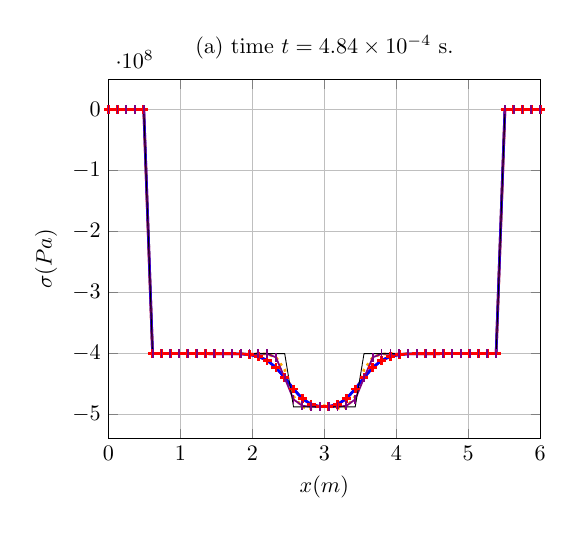
\begin{tikzpicture}[scale=0.8]
\begin{axis}[xlabel=$x (m)$,ylabel=$\sigma (Pa)$,ymajorgrids=true,xmajorgrids=true,legend pos=outer north east,title={(a) time $t = 4.84\times 10^{-4} $ s.},xmin=0.,xmax=6.]
\addplot[Red,very thick,mark=+,solid] coordinates {(0.0,-1.4032094709741823e-07) (0.12244897959183673,1.4032094709741797e-07) (0.24489795918367346,-5.501313561848306e-23) (0.36734693877551017,-1.4032094709741882e-07) (0.4897959183673469,-4.2096284129225576e-07) (0.6122448979591837,-400000000.0000052) (0.7346938775510203,-400000000.0003803) (0.8571428571428571,-400000000.0131417) (0.9795918367346939,-400000000.2874559) (1.1020408163265305,-400000004.46415013) (1.2244897959183674,-400000052.34678423) (1.346938775510204,-400000481.2046858) (1.4693877551020407,-400003554.03647596) (1.5918367346938775,-400021443.0967657) (1.7142857142857142,-400106894.9802318) (1.836734693877551,-400443646.6051052) (1.9591836734693877,-401540408.59283984) (2.0816326530612246,-404487333.2231472) (2.204081632653061,-410984305.87262785) (2.326530612244898,-422622254.02503896) (2.4489795918367347,-439299786.1010327) (2.571428571428571,-457971198.93456453) (2.693877551020408,-473710434.18348145) (2.816326530612245,-483108267.7934754) (2.9387755102040813,-486652315.1909913) (3.061224489795918,-486652315.1909913) (3.183673469387755,-483108267.7934754) (3.306122448979592,-473710434.18348145) (3.4285714285714284,-457971198.93456453) (3.5510204081632653,-439299786.1010328) (3.673469387755102,-422622254.025039) (3.7959183673469385,-410984305.8726279) (3.9183673469387754,-404487333.2231472) (4.040816326530612,-401540408.59283984) (4.163265306122449,-400443646.6051051) (4.285714285714286,-400106894.98023176) (4.408163265306122,-400021443.0967656) (4.530612244897959,-400003554.0364758) (4.653061224489796,-400000481.20468575) (4.775510204081632,-400000052.3467841) (4.8979591836734695,-400000004.46415013) (5.020408163265306,-400000000.2874559) (5.142857142857142,-400000000.01314175) (5.26530612244898,-400000000.0003803) (5.387755102040816,-400000000.0000052) (5.5102040816326525,1.403209470974181e-07) (5.63265306122449,-4.209628412922546e-07) (5.755102040816326,-7.335084749131074e-23) (5.877551020408163,-7.335084749131074e-23) (6.0,1.4032094709741816e-07) };
\addplot[Orange,very thick,mark=none,dotted] coordinates {(0.0011999999999999927,0.0) (0.12359999999999997,0.0) (0.24599999999999994,0.0) (0.36839999999999995,0.0) (0.4907999999999999,0.0) (0.6131999999999999,-399999999.9999996) (0.7355999999999999,-399999999.9999968) (0.858,-400000000.0) (0.9803999999999998,-399999999.9999996) (1.1027999999999998,-400000000.00000036) (1.2251999999999996,-400000000.0000013) (1.3475999999999997,-400000000.0000979) (1.4699999999999998,-400000000.00582314) (1.5923999999999996,-400000000.2649425) (1.7147999999999997,-400000009.2416795) (1.8371999999999995,-400000245.9026529) (1.9595999999999996,-400004932.9535555) (2.0819999999999994,-400073165.4563783) (2.2043999999999997,-400778734.27312934) (2.3267999999999995,-405684157.67745835) (2.4491999999999994,-426483554.2497189) (2.5715999999999997,-469882444.732417) (2.6939999999999995,-487460509.8573178) (2.8163999999999993,-489834934.6920107) (2.9387999999999996,-485390329.82597953) (3.0611999999999995,-485390329.8259847) (3.1835999999999993,-489834934.692009) (3.305999999999999,-487460509.85731673) (3.4283999999999994,-469882444.73241717) (3.5507999999999993,-426483554.2497191) (3.673199999999999,-405684157.67745817) (3.7955999999999994,-400778734.27312946) (3.9179999999999993,-400073165.4563784) (4.040399999999999,-400004932.95355564) (4.1628,-400000245.9026529) (4.2852,-400000009.2416795) (4.4076,-400000000.2649422) (4.53,-400000000.00582296) (4.6524,-400000000.0000977) (4.7748,-400000000.0000014) (4.8972,-400000000.00000036) (5.0196,-399999999.9999973) (5.142,-400000000.0) (5.2644,-400000000.0) (5.3868,-399999999.9999975) (5.5092,0.0) (5.6316,0.0) (5.754,0.0) (5.8764,0.0) (5.9988,0.0) };
\addplot[Blue,very thick,mark=none,solid] coordinates {(0.0011999999999999927,0.0) (0.12359999999999997,0.0) (0.24599999999999994,0.0) (0.36839999999999995,0.0) (0.4907999999999999,0.0) (0.6131999999999999,-400000000.0000052) (0.7355999999999999,-400000000.0003801) (0.858,-400000000.01314163) (0.9803999999999998,-400000000.2874559) (1.1027999999999998,-400000004.46415013) (1.2251999999999996,-400000052.3467841) (1.3475999999999997,-400000481.20468575) (1.4699999999999998,-400003554.03647584) (1.5923999999999996,-400021443.0967656) (1.7147999999999997,-400106894.9802317) (1.8371999999999995,-400443646.6051051) (1.9595999999999996,-401540408.5928399) (2.0819999999999994,-404487333.2231473) (2.2043999999999997,-410984305.8726279) (2.3267999999999995,-422622254.0250391) (2.4491999999999994,-439299786.10103285) (2.5715999999999997,-457971198.9345646) (2.6939999999999995,-473710434.1834816) (2.8163999999999993,-483108267.79347533) (2.9387999999999996,-486652315.1909914) (3.0611999999999995,-486652315.1909914) (3.1835999999999993,-483108267.79347533) (3.305999999999999,-473710434.1834816) (3.4283999999999994,-457971198.9345646) (3.5507999999999993,-439299786.10103285) (3.673199999999999,-422622254.0250391) (3.7955999999999994,-410984305.8726279) (3.9179999999999993,-404487333.2231473) (4.040399999999999,-401540408.5928399) (4.1628,-400443646.6051051) (4.2852,-400106894.9802317) (4.4076,-400021443.0967656) (4.53,-400003554.03647584) (4.6524,-400000481.20468575) (4.7748,-400000052.3467841) (4.8972,-400000004.46415013) (5.0196,-400000000.2874559) (5.142,-400000000.01314163) (5.2644,-400000000.0003801) (5.3868,-400000000.0000052) (5.5092,0.0) (5.6316,0.0) (5.754,0.0) (5.8764,0.0) (5.9988,0.0) };
\addplot[Purple,thick,mark=|,solid] coordinates {(0.0011999999999999927,0.0) (0.12359999999999997,0.0) (0.24599999999999994,0.0) (0.36839999999999995,0.0) (0.4907999999999999,0.0) (0.6131999999999999,-399999999.99999994) (0.7355999999999999,-400000000.0) (0.858,-400000000.0) (0.9803999999999998,-400000000.0) (1.1027999999999998,-400000000.0) (1.2251999999999996,-400000000.00000024) (1.3475999999999997,-400000000.00001407) (1.4699999999999998,-400000000.0007095) (1.5923999999999996,-400000000.0295273) (1.7147999999999997,-400000001.0283913) (1.8371999999999995,-400000030.33246076) (1.9595999999999996,-400000768.4378232) (2.0819999999999994,-400016975.1308303) (2.2043999999999997,-400318783.1149349) (2.3267999999999995,-405939608.94153374) (2.4491999999999994,-439871901.51192373) (2.5715999999999997,-475012040.0305417) (2.6939999999999995,-485411927.60231024) (2.8163999999999993,-487101987.7579666) (2.9387999999999996,-487278357.03341293) (3.0611999999999995,-487278357.03341293) (3.1835999999999993,-487101987.7579666) (3.305999999999999,-485411927.60231024) (3.4283999999999994,-475012040.0305417) (3.5507999999999993,-439871901.51192373) (3.673199999999999,-405939608.94153374) (3.7955999999999994,-400318783.1149349) (3.9179999999999993,-400016975.1308303) (4.040399999999999,-400000768.4378232) (4.1628,-400000030.33246076) (4.2852,-400000001.0283913) (4.4076,-400000000.0295273) (4.53,-400000000.0007095) (4.6524,-400000000.00001407) (4.7748,-400000000.0000003) (4.8972,-400000000.0) (5.0196,-400000000.0) (5.142,-400000000.0) (5.2644,-400000000.0) (5.3868,-399999999.99999994) (5.5092,0.0) (5.6316,0.0) (5.754,0.0) (5.8764,0.0) (5.9988,0.0) };
\addplot[black,thin,mark=none,solid] coordinates {(0.0,-0.0) (0.12244897959183673,-0.0) (0.24489795918367346,-0.0) (0.36734693877551017,-0.0) (0.4897959183673469,-0.0) (0.6122448979591837,-400000000.0) (0.7346938775510203,-400000000.0) (0.8571428571428571,-400000000.0) (0.9795918367346939,-400000000.0) (1.1020408163265305,-400000000.0) (1.2244897959183674,-400000000.0) (1.346938775510204,-400000000.0) (1.4693877551020407,-400000000.0) (1.5918367346938775,-400000000.0) (1.7142857142857142,-400000000.0) (1.836734693877551,-400000000.0) (1.9591836734693877,-400000000.0) (2.0816326530612246,-400000000.0) (2.204081632653061,-400000000.0) (2.326530612244898,-400000000.0) (2.4489795918367347,-400000000.0) (2.571428571428571,-487287156.09439695) (2.693877551020408,-487287156.09439695) (2.816326530612245,-487287156.09439695) (2.9387755102040813,-487287156.09439695) (3.061224489795918,-487287156.09439695) (3.183673469387755,-487287156.09439695) (3.306122448979592,-487287156.09439695) (3.4285714285714284,-487287156.09439695) (3.5510204081632653,-400000000.0) (3.673469387755102,-400000000.0) (3.7959183673469385,-400000000.0) (3.9183673469387754,-400000000.0) (4.040816326530612,-400000000.0) (4.163265306122449,-400000000.0) (4.285714285714286,-400000000.0) (4.408163265306122,-400000000.0) (4.530612244897959,-400000000.0) (4.653061224489796,-400000000.0) (4.775510204081632,-400000000.0) (4.8979591836734695,-400000000.0) (5.020408163265306,-400000000.0) (5.142857142857142,-400000000.0) (5.26530612244898,-400000000.0) (5.387755102040816,-400000000.0) (5.5102040816326525,-0.0) (5.63265306122449,-0.0) (5.755102040816326,-0.0) (5.877551020408163,-0.0) (6.0,-0.0) };
%\legend{dgmpm,fem,fvm,fvm (SB),exact}
\end{axis}
\end{tikzpicture}
%%% Local Variables:
%%% mode: latex
%%% TeX-master: "../../mainManuscript"
%%% End:
}
  % {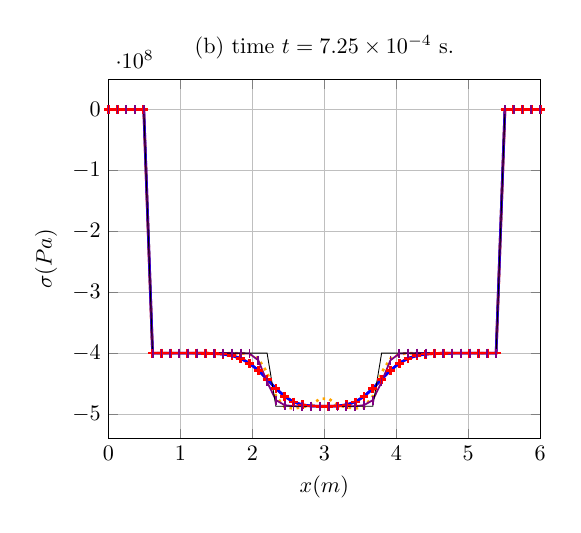
\begin{tikzpicture}[scale=0.8]
\begin{axis}[xlabel=$x (m)$,ylabel=$\sigma (Pa)$,ymajorgrids=true,xmajorgrids=true,legend pos=outer north east,title={(b) time $t = 7.25\times 10^{-4} $ s.},xmin=0.,xmax=6.]
\addplot[Red,very thick,mark=+,solid] coordinates {(0.0,-0.016398596440346053) (0.12244897959183673,-0.06425322857955201) (0.24489795918367346,-0.7380674881804443) (0.36734693877551017,-2.12047390173559) (0.4897959183673469,-28.76271861558054) (0.6122448979591837,-400000015.4159754) (0.7346938775510203,-400000102.7573024) (0.8571428571428571,-400000598.1932516) (0.9795918367346939,-400003055.79803795) (1.1020408163265305,-400013747.0436081) (1.2244897959183674,-400054602.7199052) (1.346938775510204,-400191823.2382515) (1.4693877551020407,-400596672.6802674) (1.5918367346938775,-401644186.51493835) (1.7142857142857142,-404014374.4754996) (1.836734693877551,-408684632.25449073) (1.9591836734693877,-416652037.9726774) (2.0816326530612246,-428329061.0045163) (2.204081632653061,-442879954.5361007) (2.326530612244898,-458084443.80872595) (2.4489795918367347,-471157539.9020842) (2.571428571428571,-480164339.19475454) (2.693877551020408,-484944715.5259052) (2.816326530612245,-486779650.5319825) (2.9387755102040813,-487233015.60471344) (3.061224489795918,-487233015.60471344) (3.183673469387755,-486779650.5319825) (3.306122448979592,-484944715.5259052) (3.4285714285714284,-480164339.19475454) (3.5510204081632653,-471157539.9020842) (3.673469387755102,-458084443.80872613) (3.7959183673469385,-442879954.5361007) (3.9183673469387754,-428329061.0045163) (4.040816326530612,-416652037.9726776) (4.163265306122449,-408684632.2544908) (4.285714285714286,-404014374.4754996) (4.408163265306122,-401644186.5149382) (4.530612244897959,-400596672.68026733) (4.653061224489796,-400191823.2382513) (4.775510204081632,-400054602.7199051) (4.8979591836734695,-400013747.04360807) (5.020408163265306,-400003055.79803795) (5.142857142857142,-400000598.19325155) (5.26530612244898,-400000102.75730234) (5.387755102040816,-400000015.4159754) (5.5102040816326525,-28.762718512303003) (5.63265306122449,-2.1204742438100417) (5.755102040816326,-0.7380675867576459) (5.877551020408163,-0.06425320166977637) (6.0,-0.01639854380134023) };
\addplot[Orange,very thick,mark=none,dotted] coordinates {(0.0011999999999999927,0.0) (0.12359999999999997,2.8345154836222343e-06) (0.24599999999999994,0.0) (0.36839999999999995,-5.6690309672444694e-06) (0.4907999999999999,5.563100179036459e-06) (0.6131999999999999,-400000000.00000036) (0.7355999999999999,-400000000.00000095) (0.858,-400000000.0000158) (0.9803999999999998,-400000000.000588) (1.1027999999999998,-400000000.0183558) (1.2251999999999996,-400000000.47669524) (1.3475999999999997,-400000010.242256) (1.4699999999999998,-400000180.58382314) (1.5923999999999996,-400002583.79875094) (1.7147999999999997,-400029558.11391515) (1.8371999999999995,-400265019.7421873) (1.9595999999999996,-401812442.4208182) (2.0819999999999994,-409100274.22059995) (2.2043999999999997,-431724216.84982246) (2.3267999999999995,-470516941.3021229) (2.4491999999999994,-488918339.55243546) (2.5715999999999997,-490903509.0666595) (2.6939999999999995,-488910392.160918) (2.8163999999999993,-485129466.2005724) (2.9387999999999996,-474875832.26573056) (3.0611999999999995,-474875832.26572955) (3.1835999999999993,-485129466.20057756) (3.305999999999999,-488910392.1609156) (3.4283999999999994,-490903509.0666595) (3.5507999999999993,-488918339.5524351) (3.673199999999999,-470516941.30212307) (3.7955999999999994,-431724216.8498228) (3.9179999999999993,-409100274.22060007) (4.040399999999999,-401812442.42081815) (4.1628,-400265019.742187) (4.2852,-400029558.11391526) (4.4076,-400002583.79875064) (4.53,-400000180.5838233) (4.6524,-400000010.242256) (4.7748,-400000000.47669554) (4.8972,-400000000.01835567) (5.0196,-400000000.00058854) (5.142,-400000000.00001574) (5.2644,-400000000.0000007) (5.3868,-400000000.0) (5.5092,-2.660415564296186e-06) (5.6316,-2.493917513477148e-06) (5.754,-2.7171818926536604e-06) (5.8764,3.405979701450893e-07) (5.9988,-2.8345154836222373e-06) };
\addplot[Blue,very thick,mark=none,solid] coordinates {(0.0011999999999999927,-0.00357849008468239) (0.12359999999999997,-0.06440079814818947) (0.24599999999999994,-0.21143910174666652) (0.36839999999999995,-2.1204748738318564) (0.4907999999999999,-3.2714037895202637) (0.6131999999999999,-400000015.4159753) (0.7355999999999999,-400000102.75730234) (0.858,-400000598.1932516) (0.9803999999999998,-400003055.79803795) (1.1027999999999998,-400013747.04360807) (1.2251999999999996,-400054602.7199051) (1.3475999999999997,-400191823.2382513) (1.4699999999999998,-400596672.68026733) (1.5923999999999996,-401644186.5149383) (1.7147999999999997,-404014374.47549963) (1.8371999999999995,-408684632.25449085) (1.9595999999999996,-416652037.9726776) (2.0819999999999994,-428329061.00451636) (2.2043999999999997,-442879954.5361008) (2.3267999999999995,-458084443.80872625) (2.4491999999999994,-471157539.9020842) (2.5715999999999997,-480164339.1947546) (2.6939999999999995,-484944715.52590525) (2.8163999999999993,-486779650.5319826) (2.9387999999999996,-487233015.60471344) (3.0611999999999995,-487233015.60471344) (3.1835999999999993,-486779650.5319826) (3.305999999999999,-484944715.52590525) (3.4283999999999994,-480164339.1947546) (3.5507999999999993,-471157539.9020842) (3.673199999999999,-458084443.80872625) (3.7955999999999994,-442879954.5361008) (3.9179999999999993,-428329061.00451636) (4.040399999999999,-416652037.9726776) (4.1628,-408684632.25449085) (4.2852,-404014374.47549963) (4.4076,-401644186.5149383) (4.53,-400596672.68026733) (4.6524,-400191823.2382513) (4.7748,-400054602.7199051) (4.8972,-400013747.04360807) (5.0196,-400003055.79803795) (5.142,-400000598.1932516) (5.2644,-400000102.75730234) (5.3868,-400000015.4159753) (5.5092,-3.2714037895202637) (5.6316,-2.1204748738318564) (5.754,-0.21143910174666652) (5.8764,-0.06440079814818947) (5.9988,-0.00357849008468239) };
\addplot[Purple,thick,mark=|,solid] coordinates {(0.0011999999999999927,1.6543612251060583e-24) (0.12359999999999997,1.6543612251060553e-23) (0.24599999999999994,2.452440800103604e-08) (0.36839999999999995,-3.508023677435457e-08) (0.4907999999999999,-5.960464477539063e-08) (0.6131999999999999,-400000000.0) (0.7355999999999999,-400000000.0) (0.858,-400000000.0000003) (0.9803999999999998,-400000000.0000133) (1.1027999999999998,-400000000.0004144) (1.2251999999999996,-400000000.0115142) (1.3475999999999997,-400000000.2871339) (1.4699999999999998,-400000006.46675307) (1.5923999999999996,-400000132.73197645) (1.7147999999999997,-400002510.7191475) (1.8371999999999995,-400043970.06492174) (1.9595999999999996,-400741455.361692) (2.0819999999999994,-411776022.67189264) (2.2043999999999997,-447347518.96724993) (2.3267999999999995,-477210124.05958325) (2.4491999999999994,-485453941.80645174) (2.5715999999999997,-487021615.6680456) (2.6939999999999995,-487258956.9032909) (2.8163999999999993,-487285223.6098061) (2.9387999999999996,-487287092.0986835) (3.0611999999999995,-487287092.0986835) (3.1835999999999993,-487285223.6098061) (3.305999999999999,-487258956.9032909) (3.4283999999999994,-487021615.6680456) (3.5507999999999993,-485453941.80645174) (3.673199999999999,-477210124.05958325) (3.7955999999999994,-447347518.96724993) (3.9179999999999993,-411776022.67189264) (4.040399999999999,-400741455.361692) (4.1628,-400043970.06492174) (4.2852,-400002510.71914756) (4.4076,-400000132.73197645) (4.53,-400000006.466753) (4.6524,-400000000.287134) (4.7748,-400000000.01151425) (4.8972,-400000000.0004144) (5.0196,-400000000.0000133) (5.142,-400000000.0000003) (5.2644,-400000000.0) (5.3868,-400000000.0) (5.5092,-5.960464477539063e-08) (5.6316,-3.508023677435457e-08) (5.754,2.452440800103604e-08) (5.8764,1.6543612251060553e-23) (5.9988,1.6543612251060583e-24) };
\addplot[black,thin,mark=none,solid] coordinates {(0.0,-0.0) (0.12244897959183673,-0.0) (0.24489795918367346,-0.0) (0.36734693877551017,-0.0) (0.4897959183673469,-0.0) (0.6122448979591837,-400000000.0) (0.7346938775510203,-400000000.0) (0.8571428571428571,-400000000.0) (0.9795918367346939,-400000000.0) (1.1020408163265305,-400000000.0) (1.2244897959183674,-400000000.0) (1.346938775510204,-400000000.0) (1.4693877551020407,-400000000.0) (1.5918367346938775,-400000000.0) (1.7142857142857142,-400000000.0) (1.836734693877551,-400000000.0) (1.9591836734693877,-400000000.0) (2.0816326530612246,-400000000.0) (2.204081632653061,-400000000.0) (2.326530612244898,-487287156.09439695) (2.4489795918367347,-487287156.09439695) (2.571428571428571,-487287156.09439695) (2.693877551020408,-487287156.09439695) (2.816326530612245,-487287156.09439695) (2.9387755102040813,-487287156.09439695) (3.061224489795918,-487287156.09439695) (3.183673469387755,-487287156.09439695) (3.306122448979592,-487287156.09439695) (3.4285714285714284,-487287156.09439695) (3.5510204081632653,-487287156.09439695) (3.673469387755102,-487287156.09439695) (3.7959183673469385,-400000000.0) (3.9183673469387754,-400000000.0) (4.040816326530612,-400000000.0) (4.163265306122449,-400000000.0) (4.285714285714286,-400000000.0) (4.408163265306122,-400000000.0) (4.530612244897959,-400000000.0) (4.653061224489796,-400000000.0) (4.775510204081632,-400000000.0) (4.8979591836734695,-400000000.0) (5.020408163265306,-400000000.0) (5.142857142857142,-400000000.0) (5.26530612244898,-400000000.0) (5.387755102040816,-400000000.0) (5.5102040816326525,-0.0) (5.63265306122449,-0.0) (5.755102040816326,-0.0) (5.877551020408163,-0.0) (6.0,-0.0) };
%\legend{dgmpm,fem,fvm,fvm (SB),exact}
\end{axis}
\end{tikzpicture}
%%% Local Variables:
%%% mode: latex
%%% TeX-master: "../../mainManuscript"
%%% End:
}
  {\begin{tikzpicture}[scale=.9]
\begin{groupplot}[group style={group size=3 by 2,
ylabels at=edge left, yticklabels at=edge left,horizontal sep=2.ex,
vertical sep=4ex,xticklabels at=edge bottom,xlabels at=edge bottom},
ymajorgrids=true,xmajorgrids=true,enlargelimits=0,xmin=0.,xmax=6.,xlabel=$x (m)$,
axis on top,scale only axis,width=0.32\linewidth
]
\nextgroupplot[title={(a) $t = 4.17\times 10^{-4} $ s.},ylabel=$\sigma (Pa)$,]
\addplot[Blue,solid,mark=none,very thick,mark size=2pt] coordinates{(0.0,-3.25611587112e-07) (0.122448979592,-6.54162606233e-22) (0.244897959184,0.0) (0.367346938776,3.25611587112e-07) (0.489795918367,-4.88417380668e-07) (0.612244897959,-706703995.006) (0.734693877551,-739923853.313) (0.857142857143,-818114621.328) (0.979591836735,-934350667.086) (1.10204081633,-1056745717.41) (1.22448979592,-1153785079.18) (1.34693877551,-1213891661.99) (1.4693877551,-1243675875.17) (1.59183673469,-1255667377.46) (1.71428571429,-1259628756.78) (1.83673469388,-1260708382.47) (1.95918367347,-1260951555.07) (2.08163265306,-1260996741.7) (2.20408163265,-1261003631.25) (2.32653061224,-1261004484.73) (2.44897959184,-1261004569.31) (2.57142857143,-1261004575.86) (2.69387755102,-1261004576.24) (2.81632653061,-1261004576.26) (2.9387755102,-1261004576.26) (3.0612244898,-1261004576.26) (3.18367346939,-1261004576.26) (3.30612244898,-1261004576.24) (3.42857142857,-1261004575.86) (3.55102040816,-1261004569.31) (3.67346938776,-1261004484.73) (3.79591836735,-1261003631.25) (3.91836734694,-1260996741.7) (4.04081632653,-1260951555.07) (4.16326530612,-1260708382.47) (4.28571428571,-1259628756.78) (4.40816326531,-1255667377.46) (4.5306122449,-1243675875.17) (4.65306122449,-1213891661.99) (4.77551020408,-1153785079.18) (4.89795918367,-1056745717.41) (5.02040816327,-934350667.086) (5.14285714286,-818114621.328) (5.26530612245,-739923853.313) (5.38775510204,-706703995.006) (5.51020408163,-4.88417380668e-07) (5.63265306122,0.0) (5.75510204082,-4.88417380668e-07) (5.87755102041,0.0) (6.0,-4.88417380668e-07) };
\addplot[Red,solid,mark=+,thick,mark size=2pt] coordinates{(0.0,0.0) (0.122448979592,0.0) (0.244897959184,0.0) (0.367346938776,0.0) (0.489795918367,0.0) (0.612244897959,-700099961.461) (0.734693877551,-702215400.671) (0.857142857143,-720845446.691) (0.979591836735,-807249777.224) (1.10204081633,-1021817726.09) (1.22448979592,-1257135415.88) (1.34693877551,-1201909815.27) (1.4693877551,-1284541316.1) (1.59183673469,-1197762497.59) (1.71428571429,-1280230396.14) (1.83673469388,-1230639248.48) (1.95918367347,-1232614670.29) (2.08163265306,-1296340561.14) (2.20408163265,-1163180742.37) (2.32653061224,-1344085453.29) (2.44897959184,-1125286993.99) (2.57142857143,-1354573027.57) (2.69387755102,-1144440690.69) (2.81632653061,-1331966839.32) (2.9387755102,-1234245710.89) (3.0612244898,-1234245710.89) (3.18367346939,-1331966839.32) (3.30612244898,-1144440690.69) (3.42857142857,-1354573027.57) (3.55102040816,-1125286993.99) (3.67346938776,-1344085453.29) (3.79591836735,-1163180742.37) (3.91836734694,-1296340561.14) (4.04081632653,-1232614670.29) (4.16326530612,-1230639248.48) (4.28571428571,-1280230396.14) (4.40816326531,-1197762497.59) (4.5306122449,-1284541316.1) (4.65306122449,-1201909815.27) (4.77551020408,-1257135415.88) (4.89795918367,-1021817726.09) (5.02040816327,-807249777.224) (5.14285714286,-720845446.691) (5.26530612245,-702215400.671) (5.38775510204,-700099961.461) (5.51020408163,0.0) (5.63265306122,0.0) (5.75510204082,0.0) (5.87755102041,0.0) (6.0,0.0) };
%\addplot[Blue,solid,mark=none,very thick,mark size=2pt] coordinates{(0.0,0.0) (0.122448979592,0.0) (0.244897959184,0.0) (0.367346938776,0.0) (0.489795918367,0.0) (0.612244897959,-706703995.006) (0.734693877551,-739923853.313) (0.857142857143,-818114621.328) (0.979591836735,-934350667.086) (1.10204081633,-1056745717.41) (1.22448979592,-1153785079.18) (1.34693877551,-1213891661.99) (1.4693877551,-1243675875.17) (1.59183673469,-1255667377.46) (1.71428571429,-1259628756.78) (1.83673469388,-1260708382.47) (1.95918367347,-1260951555.07) (2.08163265306,-1260996741.7) (2.20408163265,-1261003631.25) (2.32653061224,-1261004484.73) (2.44897959184,-1261004569.31) (2.57142857143,-1261004575.86) (2.69387755102,-1261004576.24) (2.81632653061,-1261004576.26) (2.9387755102,-1261004576.26) (3.0612244898,-1261004576.26) (3.18367346939,-1261004576.26) (3.30612244898,-1261004576.24) (3.42857142857,-1261004575.86) (3.55102040816,-1261004569.31) (3.67346938776,-1261004484.73) (3.79591836735,-1261003631.25) (3.91836734694,-1260996741.7) (4.04081632653,-1260951555.07) (4.16326530612,-1260708382.47) (4.28571428571,-1259628756.78) (4.40816326531,-1255667377.46) (4.5306122449,-1243675875.17) (4.65306122449,-1213891661.99) (4.77551020408,-1153785079.18) (4.89795918367,-1056745717.41) (5.02040816327,-934350667.086) (5.14285714286,-818114621.328) (5.26530612245,-739923853.313) (5.38775510204,-706703995.006) (5.51020408163,0.0) (5.63265306122,0.0) (5.75510204082,0.0) (5.87755102041,0.0) (6.0,0.0) };
\addplot[Purple,solid,mark=x,thick,mark size=2pt] coordinates{(0.0,0.0) (0.122448979592,0.0) (0.244897959184,0.0) (0.367346938776,0.0) (0.489795918367,0.0) (0.612244897959,-700149009.851) (0.734693877551,-702792255.867) (0.857142857143,-725326867.327) (0.979591836735,-850156660.853) (1.10204081633,-1109984935.97) (1.22448979592,-1250258832.44) (1.34693877551,-1260471082.96) (1.4693877551,-1260981625.99) (1.59183673469,-1261003693.9) (1.71428571429,-1261004546.97) (1.83673469388,-1261004575.43) (1.95918367347,-1261004576.24) (2.08163265306,-1261004576.26) (2.20408163265,-1261004576.26) (2.32653061224,-1261004576.26) (2.44897959184,-1261004576.26) (2.57142857143,-1261004576.26) (2.69387755102,-1261004576.26) (2.81632653061,-1261004576.26) (2.9387755102,-1261004576.26) (3.0612244898,-1261004576.26) (3.18367346939,-1261004576.26) (3.30612244898,-1261004576.26) (3.42857142857,-1261004576.26) (3.55102040816,-1261004576.26) (3.67346938776,-1261004576.26) (3.79591836735,-1261004576.26) (3.91836734694,-1261004576.26) (4.04081632653,-1261004576.24) (4.16326530612,-1261004575.43) (4.28571428571,-1261004546.97) (4.40816326531,-1261003693.9) (4.5306122449,-1260981625.99) (4.65306122449,-1260471082.96) (4.77551020408,-1250258832.44) (4.89795918367,-1109984935.97) (5.02040816327,-850156660.853) (5.14285714286,-725326867.327) (5.26530612245,-702792255.867) (5.38775510204,-700149009.851) (5.51020408163,0.0) (5.63265306122,0.0) (5.75510204082,0.0) (5.87755102041,0.0) (6.0,0.0) };
\addplot[black,solid,mark=none,thin,mark size=2pt] coordinates{(0.0,-0.0) (0.122448979592,-0.0) (0.244897959184,-0.0) (0.367346938776,-0.0) (0.489795918367,-0.0) (0.612244897959,-700000000.0) (0.734693877551,-700000000.0) (0.857142857143,-700000000.0) (0.979591836735,-700000000.0) (1.10204081633,-1261004576.26) (1.22448979592,-1261004576.26) (1.34693877551,-1261004576.26) (1.4693877551,-1261004576.26) (1.59183673469,-1261004576.26) (1.71428571429,-1261004576.26) (1.83673469388,-1261004576.26) (1.95918367347,-1261004576.26) (2.08163265306,-1261004576.26) (2.20408163265,-1261004576.26) (2.32653061224,-1261004576.26) (2.44897959184,-1261004576.26) (2.57142857143,-1261004576.26) (2.69387755102,-1261004576.26) (2.81632653061,-1261004576.26) (2.9387755102,-1261004576.26) (3.0612244898,-1261004576.26) (3.18367346939,-1261004576.26) (3.30612244898,-1261004576.26) (3.42857142857,-1261004576.26) (3.55102040816,-1261004576.26) (3.67346938776,-1261004576.26) (3.79591836735,-1261004576.26) (3.91836734694,-1261004576.26) (4.04081632653,-1261004576.26) (4.16326530612,-1261004576.26) (4.28571428571,-1261004576.26) (4.40816326531,-1261004576.26) (4.5306122449,-1261004576.26) (4.65306122449,-1261004576.26) (4.77551020408,-1261004576.26) (4.89795918367,-1261004576.26) (5.02040816327,-700000000.0) (5.14285714286,-700000000.0) (5.26530612245,-700000000.0) (5.38775510204,-700000000.0) (5.51020408163,-0.0) (5.63265306122,-0.0) (5.75510204082,-0.0) (5.87755102041,-0.0) (6.0,-0.0) };
\nextgroupplot[title={(b) $t = 6.25\times 10^{-4} $ s.},]
\addplot[Blue,solid,mark=none,very thick,mark size=2pt] coordinates{(0.0,-120597397.192) (0.122448979592,-298539345.155) (0.244897959184,-464504460.171) (0.367346938776,-546627376.356) (0.489795918367,-635546108.254) (0.612244897959,-1247334335.33) (0.734693877551,-1255980074.6) (0.857142857143,-1259371705.53) (0.979591836735,-1260535220.13) (1.10204081633,-1260885267.5) (1.22448979592,-1260977777.71) (1.34693877551,-1260999265.66) (1.4693877551,-1261003650.04) (1.59183673469,-1261004434.57) (1.71428571429,-1261004557.34) (1.83673469388,-1261004574.07) (1.95918367347,-1261004576.04) (2.08163265306,-1261004576.24) (2.20408163265,-1261004576.26) (2.32653061224,-1261004576.26) (2.44897959184,-1261004576.26) (2.57142857143,-1261004576.26) (2.69387755102,-1261004576.26) (2.81632653061,-1261004576.26) (2.9387755102,-1261004576.26) (3.0612244898,-1261004576.26) (3.18367346939,-1261004576.26) (3.30612244898,-1261004576.26) (3.42857142857,-1261004576.26) (3.55102040816,-1261004576.26) (3.67346938776,-1261004576.26) (3.79591836735,-1261004576.26) (3.91836734694,-1261004576.24) (4.04081632653,-1261004576.04) (4.16326530612,-1261004574.07) (4.28571428571,-1261004557.34) (4.40816326531,-1261004434.57) (4.5306122449,-1261003650.04) (4.65306122449,-1260999265.66) (4.77551020408,-1260977777.71) (4.89795918367,-1260885267.5) (5.02040816327,-1260535220.13) (5.14285714286,-1259371705.53) (5.26530612245,-1255980074.6) (5.38775510204,-1247334335.33) (5.51020408163,-635546108.254) (5.63265306122,-546627376.356) (5.75510204082,-464504460.171) (5.87755102041,-298539345.155) (6.0,-120597397.192) };
\addplot[Red,solid,mark=+,thick,mark size=2pt] coordinates{(0.0,-176853791.946) (0.122448979592,-378394340.717) (0.244897959184,-693239198.831) (0.367346938776,-523439989.891) (0.489795918367,-693552985.172) (0.612244897959,-1243921088.33) (0.734693877551,-1243896835.42) (0.857142857143,-1238512519.71) (0.979591836735,-1242876003.16) (1.10204081633,-1229134621.64) (1.22448979592,-1260098267.15) (1.34693877551,-1238022210.52) (1.4693877551,-1269111852.12) (1.59183673469,-1241379610.23) (1.71428571429,-1289870286.85) (1.83673469388,-1207539167.6) (1.95918367347,-1302352875.65) (2.08163265306,-1179646467.18) (2.20408163265,-1302099080.79) (2.32653061224,-1195754724.16) (2.44897959184,-1294783662.94) (2.57142857143,-1223699568.31) (2.69387755102,-1275816869.64) (2.81632653061,-1243094391.4) (2.9387755102,-1250401942.26) (3.0612244898,-1250401942.26) (3.18367346939,-1243094391.4) (3.30612244898,-1275816869.64) (3.42857142857,-1223699568.31) (3.55102040816,-1294783662.94) (3.67346938776,-1195754724.16) (3.79591836735,-1302099080.79) (3.91836734694,-1179646467.18) (4.04081632653,-1302352875.65) (4.16326530612,-1207539167.6) (4.28571428571,-1289870286.85) (4.40816326531,-1241379610.23) (4.5306122449,-1269111852.12) (4.65306122449,-1238022210.52) (4.77551020408,-1260098267.15) (4.89795918367,-1229134621.64) (5.02040816327,-1242876003.16) (5.14285714286,-1238512519.71) (5.26530612245,-1243896835.42) (5.38775510204,-1243921088.33) (5.51020408163,-693552985.172) (5.63265306122,-523439989.891) (5.75510204082,-693239198.831) (5.87755102041,-378394340.717) (6.0,-176853791.946) };
%\addplot[Blue,solid,mark=none,very thick,mark size=2pt] coordinates{(0.0,-96650988.1573) (0.122448979592,-314215597.01) (0.244897959184,-447225867.044) (0.367346938776,-549691260.458) (0.489795918367,-561200942.2) (0.612244897959,-1247334335.33) (0.734693877551,-1255980074.6) (0.857142857143,-1259371705.53) (0.979591836735,-1260535220.13) (1.10204081633,-1260885267.5) (1.22448979592,-1260977777.71) (1.34693877551,-1260999265.66) (1.4693877551,-1261003650.04) (1.59183673469,-1261004434.57) (1.71428571429,-1261004557.34) (1.83673469388,-1261004574.07) (1.95918367347,-1261004576.04) (2.08163265306,-1261004576.24) (2.20408163265,-1261004576.26) (2.32653061224,-1261004576.26) (2.44897959184,-1261004576.26) (2.57142857143,-1261004576.26) (2.69387755102,-1261004576.26) (2.81632653061,-1261004576.26) (2.9387755102,-1261004576.26) (3.0612244898,-1261004576.26) (3.18367346939,-1261004576.26) (3.30612244898,-1261004576.26) (3.42857142857,-1261004576.26) (3.55102040816,-1261004576.26) (3.67346938776,-1261004576.26) (3.79591836735,-1261004576.26) (3.91836734694,-1261004576.24) (4.04081632653,-1261004576.04) (4.16326530612,-1261004574.07) (4.28571428571,-1261004557.34) (4.40816326531,-1261004434.57) (4.5306122449,-1261003650.04) (4.65306122449,-1260999265.66) (4.77551020408,-1260977777.71) (4.89795918367,-1260885267.5) (5.02040816327,-1260535220.13) (5.14285714286,-1259371705.53) (5.26530612245,-1255980074.6) (5.38775510204,-1247334335.33) (5.51020408163,-561200942.2) (5.63265306122,-549691260.458) (5.75510204082,-447225867.044) (5.87755102041,-314215597.01) (6.0,-96650988.1573) };
\addplot[Purple,solid,mark=x,thick,mark size=2pt] coordinates{(0.0,-178085389.467) (0.122448979592,-530375739.953) (0.244897959184,-606212710.479) (0.367346938776,-629775762.979) (0.489795918367,-602317892.396) (0.612244897959,-1261002720.04) (0.734693877551,-1261004493.06) (0.857142857143,-1261004572.85) (0.979591836735,-1261004576.13) (1.10204081633,-1261004576.26) (1.22448979592,-1261004576.26) (1.34693877551,-1261004576.26) (1.4693877551,-1261004576.26) (1.59183673469,-1261004576.26) (1.71428571429,-1261004576.26) (1.83673469388,-1261004576.26) (1.95918367347,-1261004576.26) (2.08163265306,-1261004576.26) (2.20408163265,-1261004576.26) (2.32653061224,-1261004576.26) (2.44897959184,-1261004576.26) (2.57142857143,-1261004576.26) (2.69387755102,-1261004576.26) (2.81632653061,-1261004576.26) (2.9387755102,-1261004576.26) (3.0612244898,-1261004576.26) (3.18367346939,-1261004576.26) (3.30612244898,-1261004576.26) (3.42857142857,-1261004576.26) (3.55102040816,-1261004576.26) (3.67346938776,-1261004576.26) (3.79591836735,-1261004576.26) (3.91836734694,-1261004576.26) (4.04081632653,-1261004576.26) (4.16326530612,-1261004576.26) (4.28571428571,-1261004576.26) (4.40816326531,-1261004576.26) (4.5306122449,-1261004576.26) (4.65306122449,-1261004576.26) (4.77551020408,-1261004576.26) (4.89795918367,-1261004576.26) (5.02040816327,-1261004576.13) (5.14285714286,-1261004572.85) (5.26530612245,-1261004493.06) (5.38775510204,-1261002720.04) (5.51020408163,-602317892.396) (5.63265306122,-629775762.979) (5.75510204082,-606212710.479) (5.87755102041,-530375739.953) (6.0,-178085389.467) };
\addplot[black,solid,mark=none,thin,mark size=2pt] coordinates{(0.0,-0.0) (0.122448979592,-630502288.13) (0.244897959184,-630502288.13) (0.367346938776,-630502288.13) (0.489795918367,-630502288.13) (0.612244897959,-1261004576.26) (0.734693877551,-1261004576.26) (0.857142857143,-1261004576.26) (0.979591836735,-1261004576.26) (1.10204081633,-1261004576.26) (1.22448979592,-1261004576.26) (1.34693877551,-1261004576.26) (1.4693877551,-1261004576.26) (1.59183673469,-1261004576.26) (1.71428571429,-1261004576.26) (1.83673469388,-1261004576.26) (1.95918367347,-1261004576.26) (2.08163265306,-1261004576.26) (2.20408163265,-1261004576.26) (2.32653061224,-1261004576.26) (2.44897959184,-1261004576.26) (2.57142857143,-1261004576.26) (2.69387755102,-1261004576.26) (2.81632653061,-1261004576.26) (2.9387755102,-1261004576.26) (3.0612244898,-1261004576.26) (3.18367346939,-1261004576.26) (3.30612244898,-1261004576.26) (3.42857142857,-1261004576.26) (3.55102040816,-1261004576.26) (3.67346938776,-1261004576.26) (3.79591836735,-1261004576.26) (3.91836734694,-1261004576.26) (4.04081632653,-1261004576.26) (4.16326530612,-1261004576.26) (4.28571428571,-1261004576.26) (4.40816326531,-1261004576.26) (4.5306122449,-1261004576.26) (4.65306122449,-1261004576.26) (4.77551020408,-1261004576.26) (4.89795918367,-1261004576.26) (5.02040816327,-1261004576.26) (5.14285714286,-1261004576.26) (5.26530612245,-1261004576.26) (5.38775510204,-1261004576.26) (5.51020408163,-630502288.13) (5.63265306122,-630502288.13) (5.75510204082,-630502288.13) (5.87755102041,-630502288.13) (6.0,-0.0) };
\nextgroupplot[title={(c) $t = 9.38\times 10^{-4} $ s.},]
\addplot[Blue,solid,mark=none,very thick,mark size=2pt] coordinates{(0.0,-288.000337932) (0.122448979592,-2340.80496129) (0.244897959184,-6717.67363515) (0.367346938776,-31436.1854389) (0.489795918367,-82819.9714218) (0.612244897959,-326370.912329) (0.734693877551,-787154.078436) (0.857142857143,-2592039.57527) (0.979591836735,-5646941.09145) (1.10204081633,-15363721.7031) (1.22448979592,-29743749.6379) (1.34693877551,-65953645.1997) (1.4693877551,-111309952.158) (1.59183673469,-198327314.771) (1.71428571429,-286130814.567) (1.83673469388,-406728211.759) (1.95918367347,-496866659.926) (2.08163265306,-575814412.329) (2.20408163265,-612581021.556) (2.32653061224,-666589640.978) (2.44897959184,-1261004576.26) (2.57142857143,-1261004576.26) (2.69387755102,-1261004576.26) (2.81632653061,-1261004576.26) (2.9387755102,-1261004576.26) (3.0612244898,-1261004576.26) (3.18367346939,-1261004576.26) (3.30612244898,-1261004576.26) (3.42857142857,-1261004576.26) (3.55102040816,-1261004576.26) (3.67346938776,-666589640.978) (3.79591836735,-612581021.556) (3.91836734694,-575814412.329) (4.04081632653,-496866659.926) (4.16326530612,-406728211.759) (4.28571428571,-286130814.567) (4.40816326531,-198327314.771) (4.5306122449,-111309952.158) (4.65306122449,-65953645.1997) (4.77551020408,-29743749.6379) (4.89795918367,-15363721.7031) (5.02040816327,-5646941.09145) (5.14285714286,-2592039.57527) (5.26530612245,-787154.078435) (5.38775510204,-326370.912328) (5.51020408163,-82819.9714216) (5.63265306122,-31436.1854396) (5.75510204082,-6717.67363523) (5.87755102041,-2340.80496198) (6.0,-288.000337821) };
\addplot[Red,solid,mark=+,thick,mark size=2pt] coordinates{(0.0,175010887.861) (0.122448979592,-157010320.723) (0.244897959184,157731015.998) (0.367346938776,-141347084.025) (0.489795918367,117914146.107) (0.612244897959,-112262666.614) (0.734693877551,51745557.7665) (0.857142857143,-67268258.7801) (0.979591836735,25135893.7176) (1.10204081633,-51161038.2558) (1.22448979592,38244096.8773) (1.34693877551,-71286114.064) (1.4693877551,42529781.3004) (1.59183673469,-256057713.884) (1.71428571429,-344993293.731) (1.83673469388,-602082756.255) (1.95918367347,-551416188.341) (2.08163265306,-667542863.568) (2.20408163265,-569236978.915) (2.32653061224,-673381420.697) (2.44897959184,-1276652083.32) (2.57142857143,-1242412632.6) (2.69387755102,-1262303877.94) (2.81632653061,-1245296647.95) (2.9387755102,-1251720925.41) (3.0612244898,-1251720925.41) (3.18367346939,-1245296647.95) (3.30612244898,-1262303877.94) (3.42857142857,-1242412632.6) (3.55102040816,-1276652083.32) (3.67346938776,-673381420.698) (3.79591836735,-569236978.915) (3.91836734694,-667542863.568) (4.04081632653,-551416188.341) (4.16326530612,-602082756.255) (4.28571428571,-344993293.731) (4.40816326531,-256057713.884) (4.5306122449,42529781.3004) (4.65306122449,-71286114.064) (4.77551020408,38244096.8773) (4.89795918367,-51161038.2559) (5.02040816327,25135893.7176) (5.14285714286,-67268258.7801) (5.26530612245,51745557.7665) (5.38775510204,-112262666.614) (5.51020408163,117914146.107) (5.63265306122,-141347084.025) (5.75510204082,157731015.998) (5.87755102041,-157010320.723) (6.0,175010887.861) };
%\addplot[Blue,solid,mark=none,very thick,mark size=2pt] coordinates{(0.0,-672.000788774) (0.122448979592,-2317.19048543) (0.244897959184,-11624.745074) (0.367346938776,-31435.0282749) (0.489795918367,-131180.591832) (0.612244897959,-326370.866691) (0.734693877551,-1145540.96903) (0.857142857143,-2592039.57381) (0.979591836735,-7576352.57499) (1.10204081633,-15363721.7031) (1.22448979592,-36933763.6053) (1.34693877551,-65953645.1997) (1.4693877551,-128588545.286) (1.59183673469,-198327314.771) (1.71428571429,-310077223.602) (1.83673469388,-406728211.759) (1.95918367347,-512542911.781) (2.08163265306,-575814412.329) (2.20408163265,-615644905.658) (2.32653061224,-597093014.006) (2.44897959184,-1261004576.26) (2.57142857143,-1261004576.26) (2.69387755102,-1261004576.26) (2.81632653061,-1261004576.26) (2.9387755102,-1261004576.26) (3.0612244898,-1261004576.26) (3.18367346939,-1261004576.26) (3.30612244898,-1261004576.26) (3.42857142857,-1261004576.26) (3.55102040816,-1261004576.26) (3.67346938776,-597093014.006) (3.79591836735,-615644905.658) (3.91836734694,-575814412.329) (4.04081632653,-512542911.781) (4.16326530612,-406728211.759) (4.28571428571,-310077223.602) (4.40816326531,-198327314.771) (4.5306122449,-128588545.286) (4.65306122449,-65953645.1997) (4.77551020408,-36933763.6053) (4.89795918367,-15363721.7031) (5.02040816327,-7576352.57499) (5.14285714286,-2592039.57381) (5.26530612245,-1145540.96903) (5.38775510204,-326370.866691) (5.51020408163,-131180.591832) (5.63265306122,-31435.0282752) (5.75510204082,-11624.7450741) (5.87755102041,-2317.19048557) (6.0,-672.000788825) };
\addplot[Purple,solid,mark=x,thick,mark size=2pt] coordinates{(0.0,-2.25543428697e-07) (0.122448979592,-4.2534511726e-07) (0.244897959184,-1.29205915567e-05) (0.367346938776,-5.98634263291e-05) (0.489795918367,-0.00564013294006) (0.612244897959,-0.0244478781214) (0.734693877551,-1.87606962943) (0.857142857143,-7.95661496292) (0.979591836735,-503.45245952) (1.10204081633,-2086.16655273) (1.22448979592,-111480.019466) (1.34693877551,-452326.402498) (1.4693877551,-21130457.3615) (1.59183673469,-83990511.6869) (1.71428571429,-358373061.459) (1.83673469388,-536458450.926) (1.95918367347,-614366251.64) (2.08163265306,-627343167.841) (2.20408163265,-630228089.381) (2.32653061224,-602429197.287) (2.44897959184,-1261004576.26) (2.57142857143,-1261004576.26) (2.69387755102,-1261004576.26) (2.81632653061,-1261004576.26) (2.9387755102,-1261004576.26) (3.0612244898,-1261004576.26) (3.18367346939,-1261004576.26) (3.30612244898,-1261004576.26) (3.42857142857,-1261004576.26) (3.55102040816,-1261004576.26) (3.67346938776,-602429197.287) (3.79591836735,-630228089.381) (3.91836734694,-627343167.841) (4.04081632653,-614366251.64) (4.16326530612,-536458450.926) (4.28571428571,-358373061.459) (4.40816326531,-83990511.6869) (4.5306122449,-21130457.3615) (4.65306122449,-452326.402499) (4.77551020408,-111480.019466) (4.89795918367,-2086.16655258) (5.02040816327,-503.452458733) (5.14285714286,-7.95661365199) (5.26530612245,-1.87606959713) (5.38775510204,-0.0244465962211) (5.51020408163,-0.00564008555892) (5.63265306122,-6.00834800616e-05) (5.75510204082,-1.35271411582e-05) (5.87755102041,-1.61242718613e-09) (6.0,-1.72675588284e-07) };
\addplot[black,solid,mark=none,thin,mark size=2pt] coordinates{(0.0,-0.0) (0.122448979592,-0.0) (0.244897959184,-0.0) (0.367346938776,-0.0) (0.489795918367,-0.0) (0.612244897959,-0.0) (0.734693877551,-0.0) (0.857142857143,-0.0) (0.979591836735,-0.0) (1.10204081633,-0.0) (1.22448979592,-0.0) (1.34693877551,-0.0) (1.4693877551,-0.0) (1.59183673469,-0.0) (1.71428571429,-0.0) (1.83673469388,-630502288.13) (1.95918367347,-630502288.13) (2.08163265306,-630502288.13) (2.20408163265,-630502288.13) (2.32653061224,-630502288.13) (2.44897959184,-1261004576.26) (2.57142857143,-1261004576.26) (2.69387755102,-1261004576.26) (2.81632653061,-1261004576.26) (2.9387755102,-1261004576.26) (3.0612244898,-1261004576.26) (3.18367346939,-1261004576.26) (3.30612244898,-1261004576.26) (3.42857142857,-1261004576.26) (3.55102040816,-1261004576.26) (3.67346938776,-630502288.13) (3.79591836735,-630502288.13) (3.91836734694,-630502288.13) (4.04081632653,-630502288.13) (4.16326530612,-630502288.13) (4.28571428571,-0.0) (4.40816326531,-0.0) (4.5306122449,-0.0) (4.65306122449,-0.0) (4.77551020408,-0.0) (4.89795918367,-0.0) (5.02040816327,-0.0) (5.14285714286,-0.0) (5.26530612245,-0.0) (5.38775510204,-0.0) (5.51020408163,-0.0) (5.63265306122,-0.0) (5.75510204082,-0.0) (5.87755102041,-0.0) (6.0,-0.0) };
\nextgroupplot[ylabel=$\eps^p $,]
\addplot[Blue,solid,mark=none,very thick,mark size=2pt] coordinates{(0.0,0.0) (0.122448979592,0.0) (0.244897959184,0.0) (0.367346938776,0.0) (0.489795918367,0.0) (0.612244897959,-2.42678552261e-05) (0.734693877551,-0.000144520735974) (0.857142857143,-0.000427564240101) (0.979591836735,-0.000848328206646) (1.10204081633,-0.00129138721235) (1.22448979592,-0.00164266092009) (1.34693877551,-0.00186024131036) (1.4693877551,-0.00196805746667) (1.59183673469,-0.00201146561977) (1.71428571429,-0.00202580545439) (1.83673469388,-0.00202971360171) (1.95918367347,-0.00203059386449) (2.08163265306,-0.00203075743601) (2.20408163265,-0.00203078237555) (2.32653061224,-0.00203078546508) (2.44897959184,-0.00203078577127) (2.57142857143,-0.00203078579498) (2.69387755102,-0.00203078579636) (2.81632653061,-0.00203078579642) (2.9387755102,-0.00203078579642) (3.0612244898,-0.00203078579642) (3.18367346939,-0.00203078579642) (3.30612244898,-0.00203078579636) (3.42857142857,-0.00203078579498) (3.55102040816,-0.00203078577127) (3.67346938776,-0.00203078546508) (3.79591836735,-0.00203078237555) (3.91836734694,-0.00203075743601) (4.04081632653,-0.00203059386449) (4.16326530612,-0.00202971360171) (4.28571428571,-0.00202580545439) (4.40816326531,-0.00201146561977) (4.5306122449,-0.00196805746667) (4.65306122449,-0.00186024131036) (4.77551020408,-0.00164266092009) (4.89795918367,-0.00129138721235) (5.02040816327,-0.000848328206646) (5.14285714286,-0.000427564240101) (5.26530612245,-0.000144520735974) (5.38775510204,-2.42678552261e-05) (5.51020408163,0.0) (5.63265306122,0.0) (5.75510204082,0.0) (5.87755102041,0.0) (6.0,0.0) };
\addplot[Red,solid,mark=+,thick,mark size=2pt] coordinates{(0.0,0.0) (0.122448979592,0.0) (0.244897959184,0.0) (0.367346938776,0.0) (0.489795918367,0.0) (0.612244897959,-3.61851443711e-07) (0.734693877551,-8.0195499392e-06) (0.857142857143,-7.54586305539e-05) (0.979591836735,-0.000388234487688) (1.10204081633,-0.00116495104467) (1.22448979592,-0.00201677978598) (1.34693877551,-0.00210739961996) (1.4693877551,-0.00213177037456) (1.59183673469,-0.00214035741921) (1.71428571429,-0.00212247124984) (1.83673469388,-0.00212231537295) (1.95918367347,-0.00205151758829) (2.08163265306,-0.00215869886387) (2.20408163265,-0.00229323761081) (2.32653061224,-0.00238373034059) (2.44897959184,-0.00242202378243) (2.57142857143,-0.00243015270063) (2.69387755102,-0.00237762404063) (2.81632653061,-0.00229249663918) (2.9387755102,-0.00220971805446) (3.0612244898,-0.00220971805446) (3.18367346939,-0.00229249663918) (3.30612244898,-0.00237762404063) (3.42857142857,-0.00243015270063) (3.55102040816,-0.00242202378243) (3.67346938776,-0.00238373034059) (3.79591836735,-0.00229323761081) (3.91836734694,-0.00215869886387) (4.04081632653,-0.00205151758829) (4.16326530612,-0.00212231537295) (4.28571428571,-0.00212247124984) (4.40816326531,-0.00214035741921) (4.5306122449,-0.00213177037456) (4.65306122449,-0.00210739961996) (4.77551020408,-0.00201677978598) (4.89795918367,-0.00116495104467) (5.02040816327,-0.000388234487688) (5.14285714286,-7.54586305539e-05) (5.26530612245,-8.01954993918e-06) (5.38775510204,-3.61851443713e-07) (5.51020408163,0.0) (5.63265306122,0.0) (5.75510204082,0.0) (5.87755102041,0.0) (6.0,0.0) };
%\addplot[Blue,solid,mark=none,very thick,mark size=2pt] coordinates{(0.0,0.0) (0.122448979592,0.0) (0.244897959184,0.0) (0.367346938776,0.0) (0.489795918367,0.0) (0.612244897959,-2.42678552261e-05) (0.734693877551,-0.000144520735974) (0.857142857143,-0.000427564240101) (0.979591836735,-0.000848328206646) (1.10204081633,-0.00129138721235) (1.22448979592,-0.00164266092009) (1.34693877551,-0.00186024131036) (1.4693877551,-0.00196805746667) (1.59183673469,-0.00201146561977) (1.71428571429,-0.00202580545439) (1.83673469388,-0.00202971360171) (1.95918367347,-0.00203059386449) (2.08163265306,-0.00203075743601) (2.20408163265,-0.00203078237555) (2.32653061224,-0.00203078546508) (2.44897959184,-0.00203078577127) (2.57142857143,-0.00203078579498) (2.69387755102,-0.00203078579636) (2.81632653061,-0.00203078579642) (2.9387755102,-0.00203078579642) (3.0612244898,-0.00203078579642) (3.18367346939,-0.00203078579642) (3.30612244898,-0.00203078579636) (3.42857142857,-0.00203078579498) (3.55102040816,-0.00203078577127) (3.67346938776,-0.00203078546508) (3.79591836735,-0.00203078237555) (3.91836734694,-0.00203075743601) (4.04081632653,-0.00203059386449) (4.16326530612,-0.00202971360171) (4.28571428571,-0.00202580545439) (4.40816326531,-0.00201146561977) (4.5306122449,-0.00196805746667) (4.65306122449,-0.00186024131036) (4.77551020408,-0.00164266092009) (4.89795918367,-0.00129138721235) (5.02040816327,-0.000848328206646) (5.14285714286,-0.000427564240101) (5.26530612245,-0.000144520735974) (5.38775510204,-2.42678552261e-05) (5.51020408163,0.0) (5.63265306122,0.0) (5.75510204082,0.0) (5.87755102041,0.0) (6.0,0.0) };
\addplot[Purple,solid,mark=x,thick,mark size=2pt] coordinates{(0.0,0.0) (0.122448979592,0.0) (0.244897959184,0.0) (0.367346938776,0.0) (0.489795918367,0.0) (0.612244897959,-5.39402175975e-07) (0.734693877551,-1.01077135439e-05) (0.857142857143,-9.16809676992e-05) (0.979591836735,-0.00054355352345) (1.10204081633,-0.00148410836551) (1.22448979592,-0.00199188717624) (1.34693877551,-0.00202885459894) (1.4693877551,-0.00203070271851) (1.59183673469,-0.00203078260234) (1.71428571429,-0.00203078569037) (1.83673469388,-0.00203078579341) (1.95918367347,-0.00203078579635) (2.08163265306,-0.00203078579642) (2.20408163265,-0.00203078579642) (2.32653061224,-0.00203078579642) (2.44897959184,-0.00203078579642) (2.57142857143,-0.00203078579642) (2.69387755102,-0.00203078579642) (2.81632653061,-0.00203078579642) (2.9387755102,-0.00203078579642) (3.0612244898,-0.00203078579642) (3.18367346939,-0.00203078579642) (3.30612244898,-0.00203078579642) (3.42857142857,-0.00203078579642) (3.55102040816,-0.00203078579642) (3.67346938776,-0.00203078579642) (3.79591836735,-0.00203078579642) (3.91836734694,-0.00203078579642) (4.04081632653,-0.00203078579635) (4.16326530612,-0.00203078579341) (4.28571428571,-0.00203078569037) (4.40816326531,-0.00203078260234) (4.5306122449,-0.00203070271851) (4.65306122449,-0.00202885459894) (4.77551020408,-0.00199188717624) (4.89795918367,-0.00148410836551) (5.02040816327,-0.00054355352345) (5.14285714286,-9.16809676992e-05) (5.26530612245,-1.01077135439e-05) (5.38775510204,-5.39402175975e-07) (5.51020408163,0.0) (5.63265306122,0.0) (5.75510204082,0.0) (5.87755102041,0.0) (6.0,0.0) };
\addplot[black,solid,mark=none,thin,mark size=2pt] coordinates{(0.0,-0.0) (0.122448979592,-0.0) (0.244897959184,-0.0) (0.367346938776,-0.0) (0.489795918367,-0.0) (0.612244897959,-0.0) (0.734693877551,-0.0) (0.857142857143,-0.0) (0.979591836735,-0.0) (1.10204081633,-0.00203078579642) (1.22448979592,-0.00203078579642) (1.34693877551,-0.00203078579642) (1.4693877551,-0.00203078579642) (1.59183673469,-0.00203078579642) (1.71428571429,-0.00203078579642) (1.83673469388,-0.00203078579642) (1.95918367347,-0.00203078579642) (2.08163265306,-0.00203078579642) (2.20408163265,-0.00203078579642) (2.32653061224,-0.00203078579642) (2.44897959184,-0.00203078579642) (2.57142857143,-0.00203078579642) (2.69387755102,-0.00203078579642) (2.81632653061,-0.00203078579642) (2.9387755102,-0.00203078579642) (3.0612244898,-0.00203078579642) (3.18367346939,-0.00203078579642) (3.30612244898,-0.00203078579642) (3.42857142857,-0.00203078579642) (3.55102040816,-0.00203078579642) (3.67346938776,-0.00203078579642) (3.79591836735,-0.00203078579642) (3.91836734694,-0.00203078579642) (4.04081632653,-0.00203078579642) (4.16326530612,-0.00203078579642) (4.28571428571,-0.00203078579642) (4.40816326531,-0.00203078579642) (4.5306122449,-0.00203078579642) (4.65306122449,-0.00203078579642) (4.77551020408,-0.00203078579642) (4.89795918367,-0.00203078579642) (5.02040816327,-0.0) (5.14285714286,-0.0) (5.26530612245,-0.0) (5.38775510204,-0.0) (5.51020408163,-0.0) (5.63265306122,-0.0) (5.75510204082,-0.0) (5.87755102041,-0.0) (6.0,-0.0) };
\nextgroupplot[]
\addplot[Blue,solid,mark=none,very thick,mark size=2pt] coordinates{(0.0,-8.02367288935e-06) (0.122448979592,-0.000176144263873) (0.244897959184,-0.000720754269186) (0.367346938776,-0.00139199304109) (0.489795918367,-0.00181835559844) (0.612244897959,-0.00198130076139) (0.734693877551,-0.00201259755511) (0.857142857143,-0.00202487495214) (0.979591836735,-0.0020290867697) (1.10204081633,-0.0020303539095) (1.22448979592,-0.00203068878807) (1.34693877551,-0.00203076657251) (1.4693877551,-0.00203078244357) (1.59183673469,-0.00203078528353) (1.71428571429,-0.00203078572792) (1.83673469388,-0.00203078578848) (1.95918367347,-0.00203078579563) (2.08163265306,-0.00203078579635) (2.20408163265,-0.00203078579641) (2.32653061224,-0.00203078579642) (2.44897959184,-0.00203078579642) (2.57142857143,-0.00203078579642) (2.69387755102,-0.00203078579642) (2.81632653061,-0.00203078579642) (2.9387755102,-0.00203078579642) (3.0612244898,-0.00203078579642) (3.18367346939,-0.00203078579642) (3.30612244898,-0.00203078579642) (3.42857142857,-0.00203078579642) (3.55102040816,-0.00203078579642) (3.67346938776,-0.00203078579642) (3.79591836735,-0.00203078579641) (3.91836734694,-0.00203078579635) (4.04081632653,-0.00203078579563) (4.16326530612,-0.00203078578848) (4.28571428571,-0.00203078572792) (4.40816326531,-0.00203078528353) (4.5306122449,-0.00203078244357) (4.65306122449,-0.00203076657251) (4.77551020408,-0.00203068878807) (4.89795918367,-0.0020303539095) (5.02040816327,-0.0020290867697) (5.14285714286,-0.00202487495214) (5.26530612245,-0.00201259755511) (5.38775510204,-0.00198130076139) (5.51020408163,-0.00181835559844) (5.63265306122,-0.00139199304109) (5.75510204082,-0.000720754269186) (5.87755102041,-0.000176144263873) (6.0,-8.02367288935e-06) };
\addplot[Red,solid,mark=+,thick,mark size=2pt] coordinates{(0.0,-3.95561439648e-08) (0.122448979592,-9.31694826218e-06) (0.244897959184,-0.00024388789371) (0.367346938776,-0.00144259210839) (0.489795918367,-0.00204828198641) (0.612244897959,-0.00206755731038) (0.734693877551,-0.00205941579642) (0.857142857143,-0.00203726746288) (0.979591836735,-0.00208079289374) (1.10204081633,-0.00209312496223) (1.22448979592,-0.00214383415566) (1.34693877551,-0.00218203111843) (1.4693877551,-0.00221617096623) (1.59183673469,-0.00222991826569) (1.71428571429,-0.00220158132816) (1.83673469388,-0.00214830280991) (1.95918367347,-0.00218046289828) (2.08163265306,-0.00218767310207) (2.20408163265,-0.00229323761081) (2.32653061224,-0.00238373034059) (2.44897959184,-0.00242202378243) (2.57142857143,-0.00243015270063) (2.69387755102,-0.00237762404063) (2.81632653061,-0.00229249663918) (2.9387755102,-0.00220971805446) (3.0612244898,-0.00220971805446) (3.18367346939,-0.00229249663918) (3.30612244898,-0.00237762404063) (3.42857142857,-0.00243015270063) (3.55102040816,-0.00242202378243) (3.67346938776,-0.00238373034059) (3.79591836735,-0.00229323761081) (3.91836734694,-0.00218767310207) (4.04081632653,-0.00218046289828) (4.16326530612,-0.00214830280991) (4.28571428571,-0.00220158132816) (4.40816326531,-0.00222991826569) (4.5306122449,-0.00221617096623) (4.65306122449,-0.00218203111843) (4.77551020408,-0.00214383415566) (4.89795918367,-0.00209312496223) (5.02040816327,-0.00208079289374) (5.14285714286,-0.00203726746288) (5.26530612245,-0.00205941579642) (5.38775510204,-0.00206755731038) (5.51020408163,-0.00204828198641) (5.63265306122,-0.00144259210839) (5.75510204082,-0.00024388789371) (5.87755102041,-9.31694826217e-06) (6.0,-3.95561439667e-08) };
%\addplot[Blue,solid,mark=none,very thick,mark size=2pt] coordinates{(0.0,-8.02367288935e-06) (0.122448979592,-0.000176144263873) (0.244897959184,-0.000720754269186) (0.367346938776,-0.00139199304109) (0.489795918367,-0.00181835559844) (0.612244897959,-0.00198130076139) (0.734693877551,-0.00201259755511) (0.857142857143,-0.00202487495214) (0.979591836735,-0.0020290867697) (1.10204081633,-0.0020303539095) (1.22448979592,-0.00203068878807) (1.34693877551,-0.00203076657251) (1.4693877551,-0.00203078244357) (1.59183673469,-0.00203078528353) (1.71428571429,-0.00203078572792) (1.83673469388,-0.00203078578848) (1.95918367347,-0.00203078579563) (2.08163265306,-0.00203078579635) (2.20408163265,-0.00203078579641) (2.32653061224,-0.00203078579642) (2.44897959184,-0.00203078579642) (2.57142857143,-0.00203078579642) (2.69387755102,-0.00203078579642) (2.81632653061,-0.00203078579642) (2.9387755102,-0.00203078579642) (3.0612244898,-0.00203078579642) (3.18367346939,-0.00203078579642) (3.30612244898,-0.00203078579642) (3.42857142857,-0.00203078579642) (3.55102040816,-0.00203078579642) (3.67346938776,-0.00203078579642) (3.79591836735,-0.00203078579641) (3.91836734694,-0.00203078579635) (4.04081632653,-0.00203078579563) (4.16326530612,-0.00203078578848) (4.28571428571,-0.00203078572792) (4.40816326531,-0.00203078528353) (4.5306122449,-0.00203078244357) (4.65306122449,-0.00203076657251) (4.77551020408,-0.00203068878807) (4.89795918367,-0.0020303539095) (5.02040816327,-0.0020290867697) (5.14285714286,-0.00202487495214) (5.26530612245,-0.00201259755511) (5.38775510204,-0.00198130076139) (5.51020408163,-0.00181835559844) (5.63265306122,-0.00139199304109) (5.75510204082,-0.000720754269186) (5.87755102041,-0.000176144263873) (6.0,-8.02367288935e-06) };
\addplot[Purple,solid,mark=x,thick,mark size=2pt] coordinates{(0.0,-5.89652756596e-08) (0.122448979592,-1.01752154341e-05) (0.244897959184,-0.000302905940916) (0.367346938776,-0.00176026062723) (0.489795918367,-0.00202932889761) (0.612244897959,-0.00203077907708) (0.734693877551,-0.00203078549523) (0.857142857143,-0.00203078578407) (0.979591836735,-0.00203078579596) (1.10204081633,-0.0020307857964) (1.22448979592,-0.00203078579642) (1.34693877551,-0.00203078579642) (1.4693877551,-0.00203078579642) (1.59183673469,-0.00203078579642) (1.71428571429,-0.00203078579642) (1.83673469388,-0.00203078579642) (1.95918367347,-0.00203078579642) (2.08163265306,-0.00203078579642) (2.20408163265,-0.00203078579642) (2.32653061224,-0.00203078579642) (2.44897959184,-0.00203078579642) (2.57142857143,-0.00203078579642) (2.69387755102,-0.00203078579642) (2.81632653061,-0.00203078579642) (2.9387755102,-0.00203078579642) (3.0612244898,-0.00203078579642) (3.18367346939,-0.00203078579642) (3.30612244898,-0.00203078579642) (3.42857142857,-0.00203078579642) (3.55102040816,-0.00203078579642) (3.67346938776,-0.00203078579642) (3.79591836735,-0.00203078579642) (3.91836734694,-0.00203078579642) (4.04081632653,-0.00203078579642) (4.16326530612,-0.00203078579642) (4.28571428571,-0.00203078579642) (4.40816326531,-0.00203078579642) (4.5306122449,-0.00203078579642) (4.65306122449,-0.00203078579642) (4.77551020408,-0.00203078579642) (4.89795918367,-0.0020307857964) (5.02040816327,-0.00203078579596) (5.14285714286,-0.00203078578407) (5.26530612245,-0.00203078549523) (5.38775510204,-0.00203077907708) (5.51020408163,-0.00202932889761) (5.63265306122,-0.00176026062723) (5.75510204082,-0.000302905940916) (5.87755102041,-1.01752154341e-05) (6.0,-5.89652756596e-08) };
\addplot[black,solid,mark=none,thin,mark size=2pt] coordinates{(0.0,-0.0) (0.122448979592,-0.0) (0.244897959184,-0.0) (0.367346938776,-0.00203078579642) (0.489795918367,-0.00203078579642) (0.612244897959,-0.00203078579642) (0.734693877551,-0.00203078579642) (0.857142857143,-0.00203078579642) (0.979591836735,-0.00203078579642) (1.10204081633,-0.00203078579642) (1.22448979592,-0.00203078579642) (1.34693877551,-0.00203078579642) (1.4693877551,-0.00203078579642) (1.59183673469,-0.00203078579642) (1.71428571429,-0.00203078579642) (1.83673469388,-0.00203078579642) (1.95918367347,-0.00203078579642) (2.08163265306,-0.00203078579642) (2.20408163265,-0.00203078579642) (2.32653061224,-0.00203078579642) (2.44897959184,-0.00203078579642) (2.57142857143,-0.00203078579642) (2.69387755102,-0.00203078579642) (2.81632653061,-0.00203078579642) (2.9387755102,-0.00203078579642) (3.0612244898,-0.00203078579642) (3.18367346939,-0.00203078579642) (3.30612244898,-0.00203078579642) (3.42857142857,-0.00203078579642) (3.55102040816,-0.00203078579642) (3.67346938776,-0.00203078579642) (3.79591836735,-0.00203078579642) (3.91836734694,-0.00203078579642) (4.04081632653,-0.00203078579642) (4.16326530612,-0.00203078579642) (4.28571428571,-0.00203078579642) (4.40816326531,-0.00203078579642) (4.5306122449,-0.00203078579642) (4.65306122449,-0.00203078579642) (4.77551020408,-0.00203078579642) (4.89795918367,-0.00203078579642) (5.02040816327,-0.00203078579642) (5.14285714286,-0.00203078579642) (5.26530612245,-0.00203078579642) (5.38775510204,-0.00203078579642) (5.51020408163,-0.00203078579642) (5.63265306122,-0.00203078579642) (5.75510204082,-0.0) (5.87755102041,-0.0) (6.0,-0.0) };
\nextgroupplot[legend style={at={($(0.12,-0.45)+(0.cm,1cm)$)},legend columns=5}]
\addplot[Blue,solid,mark=none,very thick,mark size=2pt] coordinates{(0.0,-8.02367288935e-06) (0.122448979592,-0.000176144263873) (0.244897959184,-0.000720754269186) (0.367346938776,-0.00139199304109) (0.489795918367,-0.00181835559844) (0.612244897959,-0.00198130076139) (0.734693877551,-0.00202243709213) (0.857142857143,-0.00202973458775) (0.979591836735,-0.00203068454071) (1.10204081633,-0.00203077818689) (1.22448979592,-0.00203078534335) (1.34693877551,-0.00203078577479) (1.4693877551,-0.00203078579558) (1.59183673469,-0.00203078579639) (1.71428571429,-0.00203078579642) (1.83673469388,-0.00203078579642) (1.95918367347,-0.00203078579642) (2.08163265306,-0.00203078579642) (2.20408163265,-0.00203078579642) (2.32653061224,-0.00203078579642) (2.44897959184,-0.00203078579642) (2.57142857143,-0.00203078579642) (2.69387755102,-0.00203078579642) (2.81632653061,-0.00203078579642) (2.9387755102,-0.00203078579642) (3.0612244898,-0.00203078579642) (3.18367346939,-0.00203078579642) (3.30612244898,-0.00203078579642) (3.42857142857,-0.00203078579642) (3.55102040816,-0.00203078579642) (3.67346938776,-0.00203078579642) (3.79591836735,-0.00203078579642) (3.91836734694,-0.00203078579642) (4.04081632653,-0.00203078579642) (4.16326530612,-0.00203078579642) (4.28571428571,-0.00203078579642) (4.40816326531,-0.00203078579639) (4.5306122449,-0.00203078579558) (4.65306122449,-0.00203078577479) (4.77551020408,-0.00203078534335) (4.89795918367,-0.00203077818689) (5.02040816327,-0.00203068454071) (5.14285714286,-0.00202973458775) (5.26530612245,-0.00202243709213) (5.38775510204,-0.00198130076139) (5.51020408163,-0.00181835559844) (5.63265306122,-0.00139199304109) (5.75510204082,-0.000720754269186) (5.87755102041,-0.000176144263873) (6.0,-8.02367288935e-06) };
\addplot[Red,solid,mark=+,thick,mark size=2pt] coordinates{(0.0,-3.95561439648e-08) (0.122448979592,-9.31694826218e-06) (0.244897959184,-0.00024388789371) (0.367346938776,-0.00144259210839) (0.489795918367,-0.00197917145232) (0.612244897959,-0.00196963850213) (0.734693877551,-0.00195904673962) (0.857142857143,-0.00200215941238) (0.979591836735,-0.00208079289374) (1.10204081633,-0.00212841528845) (1.22448979592,-0.00219993582018) (1.34693877551,-0.00225701526709) (1.4693877551,-0.00228971920569) (1.59183673469,-0.00229544671822) (1.71428571429,-0.00227329357173) (1.83673469388,-0.00224127928973) (1.95918367347,-0.00219880778953) (2.08163265306,-0.00218767310207) (2.20408163265,-0.00229323761081) (2.32653061224,-0.00238373034059) (2.44897959184,-0.00242202378243) (2.57142857143,-0.00243015270063) (2.69387755102,-0.00237762404063) (2.81632653061,-0.00229249663918) (2.9387755102,-0.00220971805446) (3.0612244898,-0.00220971805446) (3.18367346939,-0.00229249663918) (3.30612244898,-0.00237762404063) (3.42857142857,-0.00243015270063) (3.55102040816,-0.00242202378243) (3.67346938776,-0.00238373034059) (3.79591836735,-0.00229323761081) (3.91836734694,-0.00218767310207) (4.04081632653,-0.00219880778953) (4.16326530612,-0.00224127928973) (4.28571428571,-0.00227329357173) (4.40816326531,-0.00229544671822) (4.5306122449,-0.00228971920569) (4.65306122449,-0.00225701526709) (4.77551020408,-0.00219993582018) (4.89795918367,-0.00212841528845) (5.02040816327,-0.00208079289374) (5.14285714286,-0.00200215941238) (5.26530612245,-0.00195904673962) (5.38775510204,-0.00196963850213) (5.51020408163,-0.00197917145232) (5.63265306122,-0.00144259210839) (5.75510204082,-0.00024388789371) (5.87755102041,-9.31694826217e-06) (6.0,-3.95561439667e-08) };
%\addplot[Blue,solid,mark=none,very thick,mark size=2pt] coordinates{(0.0,-8.02367288935e-06) (0.122448979592,-0.000176144263873) (0.244897959184,-0.000720754269186) (0.367346938776,-0.00139199304109) (0.489795918367,-0.00181835559844) (0.612244897959,-0.00198130076139) (0.734693877551,-0.00202243709213) (0.857142857143,-0.00202973458775) (0.979591836735,-0.00203068454071) (1.10204081633,-0.00203077818689) (1.22448979592,-0.00203078534335) (1.34693877551,-0.00203078577479) (1.4693877551,-0.00203078579558) (1.59183673469,-0.00203078579639) (1.71428571429,-0.00203078579642) (1.83673469388,-0.00203078579642) (1.95918367347,-0.00203078579642) (2.08163265306,-0.00203078579642) (2.20408163265,-0.00203078579642) (2.32653061224,-0.00203078579642) (2.44897959184,-0.00203078579642) (2.57142857143,-0.00203078579642) (2.69387755102,-0.00203078579642) (2.81632653061,-0.00203078579642) (2.9387755102,-0.00203078579642) (3.0612244898,-0.00203078579642) (3.18367346939,-0.00203078579642) (3.30612244898,-0.00203078579642) (3.42857142857,-0.00203078579642) (3.55102040816,-0.00203078579642) (3.67346938776,-0.00203078579642) (3.79591836735,-0.00203078579642) (3.91836734694,-0.00203078579642) (4.04081632653,-0.00203078579642) (4.16326530612,-0.00203078579642) (4.28571428571,-0.00203078579642) (4.40816326531,-0.00203078579639) (4.5306122449,-0.00203078579558) (4.65306122449,-0.00203078577479) (4.77551020408,-0.00203078534335) (4.89795918367,-0.00203077818689) (5.02040816327,-0.00203068454071) (5.14285714286,-0.00202973458775) (5.26530612245,-0.00202243709213) (5.38775510204,-0.00198130076139) (5.51020408163,-0.00181835559844) (5.63265306122,-0.00139199304109) (5.75510204082,-0.000720754269186) (5.87755102041,-0.000176144263873) (6.0,-8.02367288935e-06) };
\addplot[Purple,solid,mark=x,thick,mark size=2pt] coordinates{(0.0,-5.89652756596e-08) (0.122448979592,-1.01752154341e-05) (0.244897959184,-0.000302905940916) (0.367346938776,-0.00176026062723) (0.489795918367,-0.00202932889761) (0.612244897959,-0.00203077907708) (0.734693877551,-0.00203078577079) (0.857142857143,-0.00203078579634) (0.979591836735,-0.00203078579642) (1.10204081633,-0.00203078579642) (1.22448979592,-0.00203078579642) (1.34693877551,-0.00203078579642) (1.4693877551,-0.00203078579642) (1.59183673469,-0.00203078579642) (1.71428571429,-0.00203078579642) (1.83673469388,-0.00203078579642) (1.95918367347,-0.00203078579642) (2.08163265306,-0.00203078579642) (2.20408163265,-0.00203078579642) (2.32653061224,-0.00203078579642) (2.44897959184,-0.00203078579642) (2.57142857143,-0.00203078579642) (2.69387755102,-0.00203078579642) (2.81632653061,-0.00203078579642) (2.9387755102,-0.00203078579642) (3.0612244898,-0.00203078579642) (3.18367346939,-0.00203078579642) (3.30612244898,-0.00203078579642) (3.42857142857,-0.00203078579642) (3.55102040816,-0.00203078579642) (3.67346938776,-0.00203078579642) (3.79591836735,-0.00203078579642) (3.91836734694,-0.00203078579642) (4.04081632653,-0.00203078579642) (4.16326530612,-0.00203078579642) (4.28571428571,-0.00203078579642) (4.40816326531,-0.00203078579642) (4.5306122449,-0.00203078579642) (4.65306122449,-0.00203078579642) (4.77551020408,-0.00203078579642) (4.89795918367,-0.00203078579642) (5.02040816327,-0.00203078579642) (5.14285714286,-0.00203078579634) (5.26530612245,-0.00203078577079) (5.38775510204,-0.00203077907708) (5.51020408163,-0.00202932889761) (5.63265306122,-0.00176026062723) (5.75510204082,-0.000302905940916) (5.87755102041,-1.01752154341e-05) (6.0,-5.89652756596e-08) };
\addplot[black,solid,mark=none,thin,mark size=2pt] coordinates{(0.0,-0.0) (0.122448979592,-0.0) (0.244897959184,-0.0) (0.367346938776,-0.00203078579642) (0.489795918367,-0.00203078579642) (0.612244897959,-0.00203078579642) (0.734693877551,-0.00203078579642) (0.857142857143,-0.00203078579642) (0.979591836735,-0.00203078579642) (1.10204081633,-0.00203078579642) (1.22448979592,-0.00203078579642) (1.34693877551,-0.00203078579642) (1.4693877551,-0.00203078579642) (1.59183673469,-0.00203078579642) (1.71428571429,-0.00203078579642) (1.83673469388,-0.00203078579642) (1.95918367347,-0.00203078579642) (2.08163265306,-0.00203078579642) (2.20408163265,-0.00203078579642) (2.32653061224,-0.00203078579642) (2.44897959184,-0.00203078579642) (2.57142857143,-0.00203078579642) (2.69387755102,-0.00203078579642) (2.81632653061,-0.00203078579642) (2.9387755102,-0.00203078579642) (3.0612244898,-0.00203078579642) (3.18367346939,-0.00203078579642) (3.30612244898,-0.00203078579642) (3.42857142857,-0.00203078579642) (3.55102040816,-0.00203078579642) (3.67346938776,-0.00203078579642) (3.79591836735,-0.00203078579642) (3.91836734694,-0.00203078579642) (4.04081632653,-0.00203078579642) (4.16326530612,-0.00203078579642) (4.28571428571,-0.00203078579642) (4.40816326531,-0.00203078579642) (4.5306122449,-0.00203078579642) (4.65306122449,-0.00203078579642) (4.77551020408,-0.00203078579642) (4.89795918367,-0.00203078579642) (5.02040816327,-0.00203078579642) (5.14285714286,-0.00203078579642) (5.26530612245,-0.00203078579642) (5.38775510204,-0.00203078579642) (5.51020408163,-0.00203078579642) (5.63265306122,-0.00203078579642) (5.75510204082,-0.0) (5.87755102041,-0.0) (6.0,-0.0) };
\addlegendentry{dgmpm}
\addlegendentry{fem}
%\addlegendentry{fvm}
\addlegendentry{fvm (SB)}
\addlegendentry{exact}

\end{groupplot}
\end{tikzpicture}
%%% Local Variables:
%%% mode: latex
%%% TeX-master: "../../mainManuscript"
%%% End:
}
  \caption{elastic-plastic RP stress}
  \label{fig:stress_elastoplastic_RP}
\end{figure}
% \begin{figure}[h!]
%   \centering
%   {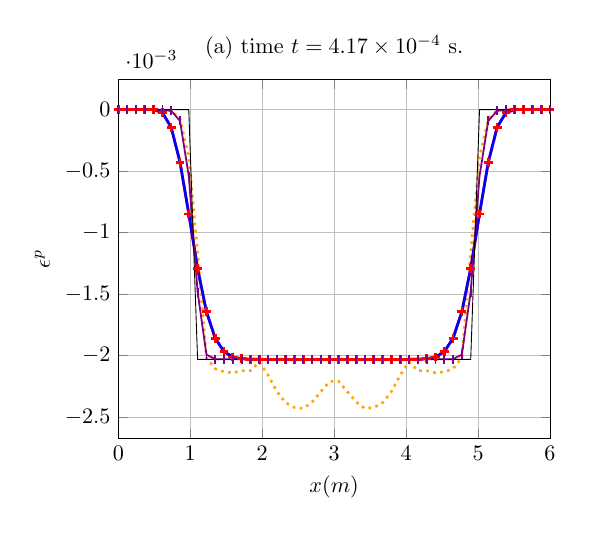
\begin{tikzpicture}[scale=0.8]
\begin{axis}[xlabel=$x (m)$,ylabel=$\epsilon^p$,ymajorgrids=true,xmajorgrids=true,legend pos=outer north east,title={(a) time $t = 4.17\times 10^{-4} $ s.},xmin=0.,xmax=6.]
\addplot[Red,very thick,mark=+,solid] coordinates {(0.0,0.0) (0.12244897959183673,0.0) (0.24489795918367346,0.0) (0.36734693877551017,0.0) (0.4897959183673469,0.0) (0.6122448979591837,-2.4267855226065594e-05) (0.7346938775510203,-0.00014452073597361284) (0.8571428571428571,-0.0004275642401009131) (0.9795918367346939,-0.0008483282066457896) (1.1020408163265305,-0.0012913872123487611) (1.2244897959183674,-0.001642660920094959) (1.346938775510204,-0.0018602413103573651) (1.4693877551020407,-0.0019680574666657586) (1.5918367346938775,-0.00201146561977191) (1.7142857142857142,-0.002025805454394895) (1.836734693877551,-0.0020297136017104972) (1.9591836734693877,-0.002030593864489664) (2.0816326530612246,-0.002030757436013639) (2.204081632653061,-0.0020307823755532774) (2.326530612244898,-0.002030785465084119) (2.4489795918367347,-0.0020307857712710334) (2.571428571428571,-0.00203078579497771) (2.693877551020408,-0.0020307857963597366) (2.816326530612245,-0.002030785796416807) (2.9387755102040813,-0.002030785796418294) (3.061224489795918,-0.002030785796418294) (3.183673469387755,-0.0020307857964168056) (3.306122448979592,-0.002030785796359739) (3.4285714285714284,-0.0020307857949777124) (3.5510204081632653,-0.002030785771271032) (3.673469387755102,-0.002030785465084119) (3.7959183673469385,-0.002030782375553277) (3.9183673469387754,-0.0020307574360136386) (4.040816326530612,-0.002030593864489664) (4.163265306122449,-0.0020297136017104964) (4.285714285714286,-0.0020258054543948927) (4.408163265306122,-0.002011465619771909) (4.530612244897959,-0.0019680574666657573) (4.653061224489796,-0.0018602413103573651) (4.775510204081632,-0.0016426609200949592) (4.8979591836734695,-0.001291387212348762) (5.020408163265306,-0.0008483282066457893) (5.142857142857142,-0.00042756424010091193) (5.26530612244898,-0.00014452073597361384) (5.387755102040816,-2.4267855226067292e-05) (5.5102040816326525,0.0) (5.63265306122449,0.0) (5.755102040816326,0.0) (5.877551020408163,0.0) (6.0,0.0) };
\addplot[Orange,very thick,mark=none,dotted] coordinates {(0.0011999999999999927,0.0) (0.12359999999999997,0.0) (0.24599999999999994,0.0) (0.36839999999999995,0.0) (0.4907999999999999,0.0) (0.6131999999999999,-3.6185144371068533e-07) (0.7355999999999999,-8.019549939201378e-06) (0.858,-7.545863055389513e-05) (0.9803999999999998,-0.00038823448768833166) (1.1027999999999998,-0.0011649510446652884) (1.2251999999999996,-0.0020167797859788647) (1.3475999999999997,-0.002107399619958115) (1.4699999999999998,-0.002131770374563102) (1.5923999999999996,-0.0021403574192086572) (1.7147999999999997,-0.0021224712498380525) (1.8371999999999995,-0.0021223153729543927) (1.9595999999999996,-0.002051517588290279) (2.0819999999999994,-0.00215869886386764) (2.2043999999999997,-0.00229323761080671) (2.3267999999999995,-0.002383730340592019) (2.4491999999999994,-0.002422023782426279) (2.5715999999999997,-0.0024301527006305407) (2.6939999999999995,-0.0023776240406298606) (2.8163999999999993,-0.0022924966391795762) (2.9387999999999996,-0.002209718054457858) (3.0611999999999995,-0.002209718054457853) (3.1835999999999993,-0.00229249663917957) (3.305999999999999,-0.002377624040629834) (3.4283999999999994,-0.0024301527006305133) (3.5507999999999993,-0.0024220237824262893) (3.673199999999999,-0.0023837303405920274) (3.7955999999999994,-0.0022932376108067225) (3.9179999999999993,-0.002158698863867652) (4.040399999999999,-0.0020515175882902612) (4.1628,-0.00212231537295439) (4.2852,-0.002122471249838043) (4.4076,-0.002140357419208655) (4.53,-0.0021317703745630944) (4.6524,-0.0021073996199581038) (4.7748,-0.002016779785978835) (4.8972,-0.0011649510446653149) (5.0196,-0.00038823448768831226) (5.142,-7.54586305539126e-05) (5.2644,-8.019549939178096e-06) (5.3868,-3.6185144371335306e-07) (5.5092,0.0) (5.6316,0.0) (5.754,0.0) (5.8764,0.0) (5.9988,0.0) };
\addplot[Blue,very thick,mark=none,solid] coordinates {(0.0011999999999999927,0.0) (0.12359999999999997,0.0) (0.24599999999999994,0.0) (0.36839999999999995,0.0) (0.4907999999999999,0.0) (0.6131999999999999,-2.4267855226066533e-05) (0.7355999999999999,-0.00014452073597361162) (0.858,-0.0004275642401009113) (0.9803999999999998,-0.0008483282066457879) (1.1027999999999998,-0.0012913872123487594) (1.2251999999999996,-0.0016426609200949575) (1.3475999999999997,-0.0018602413103573636) (1.4699999999999998,-0.0019680574666657573) (1.5923999999999996,-0.002011465619771908) (1.7147999999999997,-0.002025805454394894) (1.8371999999999995,-0.0020297136017104955) (1.9595999999999996,-0.0020305938644896646) (2.0819999999999994,-0.002030757436013637) (2.2043999999999997,-0.002030782375553278) (2.3267999999999995,-0.002030785465084118) (2.4491999999999994,-0.0020307857712710316) (2.5715999999999997,-0.002030785794977712) (2.6939999999999995,-0.002030785796359737) (2.8163999999999993,-0.002030785796416805) (2.9387999999999996,-0.0020307857964182922) (3.0611999999999995,-0.0020307857964182935) (3.1835999999999993,-0.002030785796416805) (3.305999999999999,-0.002030785796359737) (3.4283999999999994,-0.002030785794977712) (3.5507999999999993,-0.0020307857712710316) (3.673199999999999,-0.0020307854650841186) (3.7955999999999994,-0.002030782375553278) (3.9179999999999993,-0.002030757436013637) (4.040399999999999,-0.0020305938644896646) (4.1628,-0.0020297136017104955) (4.2852,-0.002025805454394893) (4.4076,-0.002011465619771907) (4.53,-0.0019680574666657573) (4.6524,-0.0018602413103573636) (4.7748,-0.0016426609200949566) (4.8972,-0.0012913872123487594) (5.0196,-0.0008483282066457876) (5.142,-0.0004275642401009109) (5.2644,-0.00014452073597361162) (5.3868,-2.4267855226066533e-05) (5.5092,0.0) (5.6316,0.0) (5.754,0.0) (5.8764,0.0) (5.9988,0.0) };
\addplot[Purple,thick,mark=|,solid] coordinates {(0.0011999999999999927,0.0) (0.12359999999999997,0.0) (0.24599999999999994,0.0) (0.36839999999999995,0.0) (0.4907999999999999,0.0) (0.6131999999999999,-5.394021759754931e-07) (0.7355999999999999,-1.010771354391672e-05) (0.858,-9.168096769918878e-05) (0.9803999999999998,-0.0005435535234499527) (1.1027999999999998,-0.0014841083655069223) (1.2251999999999996,-0.001991887176242578) (1.3475999999999997,-0.002028854598935097) (1.4699999999999998,-0.0020307027185062754) (1.5923999999999996,-0.002030782602337539) (1.7147999999999997,-0.0020307856903745234) (1.8371999999999995,-0.002030785793411752) (1.9595999999999996,-0.002030785796346042) (2.0819999999999994,-0.002030785796416862) (2.2043999999999997,-0.002030785796418289) (2.3267999999999995,-0.0020307857964183135) (2.4491999999999994,-0.0020307857964183135) (2.5715999999999997,-0.0020307857964183135) (2.6939999999999995,-0.0020307857964183135) (2.8163999999999993,-0.0020307857964183135) (2.9387999999999996,-0.0020307857964183135) (3.0611999999999995,-0.0020307857964183135) (3.1835999999999993,-0.0020307857964183135) (3.305999999999999,-0.0020307857964183126) (3.4283999999999994,-0.0020307857964183135) (3.5507999999999993,-0.0020307857964183126) (3.673199999999999,-0.0020307857964183126) (3.7955999999999994,-0.002030785796418291) (3.9179999999999993,-0.0020307857964168632) (4.040399999999999,-0.0020307857963460427) (4.1628,-0.0020307857934117523) (4.2852,-0.002030785690374525) (4.4076,-0.0020307826023375384) (4.53,-0.0020307027185062733) (4.6524,-0.002028854598935106) (4.7748,-0.0019918871762425686) (4.8972,-0.0014841083655069208) (5.0196,-0.0005435535234499549) (5.142,-9.168096769918878e-05) (5.2644,-1.010771354391672e-05) (5.3868,-5.394021759754931e-07) (5.5092,0.0) (5.6316,0.0) (5.754,0.0) (5.8764,0.0) (5.9988,0.0) };
\addplot[black,thin,mark=none,solid] coordinates {(0.0,-0.0) (0.12244897959183673,-0.0) (0.24489795918367346,-0.0) (0.36734693877551017,-0.0) (0.4897959183673469,-0.0) (0.6122448979591837,-0.0) (0.7346938775510203,-0.0) (0.8571428571428571,-0.0) (0.9795918367346939,-0.0) (1.1020408163265305,-0.002030785796418313) (1.2244897959183674,-0.002030785796418313) (1.346938775510204,-0.002030785796418313) (1.4693877551020407,-0.002030785796418313) (1.5918367346938775,-0.002030785796418313) (1.7142857142857142,-0.002030785796418313) (1.836734693877551,-0.002030785796418313) (1.9591836734693877,-0.002030785796418313) (2.0816326530612246,-0.002030785796418313) (2.204081632653061,-0.002030785796418313) (2.326530612244898,-0.002030785796418313) (2.4489795918367347,-0.002030785796418313) (2.571428571428571,-0.002030785796418313) (2.693877551020408,-0.002030785796418313) (2.816326530612245,-0.002030785796418313) (2.9387755102040813,-0.002030785796418313) (3.061224489795918,-0.002030785796418313) (3.183673469387755,-0.002030785796418313) (3.306122448979592,-0.002030785796418313) (3.4285714285714284,-0.002030785796418313) (3.5510204081632653,-0.002030785796418313) (3.673469387755102,-0.002030785796418313) (3.7959183673469385,-0.002030785796418313) (3.9183673469387754,-0.002030785796418313) (4.040816326530612,-0.002030785796418313) (4.163265306122449,-0.002030785796418313) (4.285714285714286,-0.002030785796418313) (4.408163265306122,-0.002030785796418313) (4.530612244897959,-0.002030785796418313) (4.653061224489796,-0.002030785796418313) (4.775510204081632,-0.002030785796418313) (4.8979591836734695,-0.002030785796418313) (5.020408163265306,-0.0) (5.142857142857142,-0.0) (5.26530612244898,-0.0) (5.387755102040816,-0.0) (5.5102040816326525,-0.0) (5.63265306122449,-0.0) (5.755102040816326,-0.0) (5.877551020408163,-0.0) (6.0,-0.0) };
%\legend{dgmpm,fem,fvm,fvm (SB),exact}
\end{axis}
\end{tikzpicture}
%%% Local Variables:
%%% mode: latex
%%% TeX-master: "../../mainManuscript"
%%% End:
}
%   {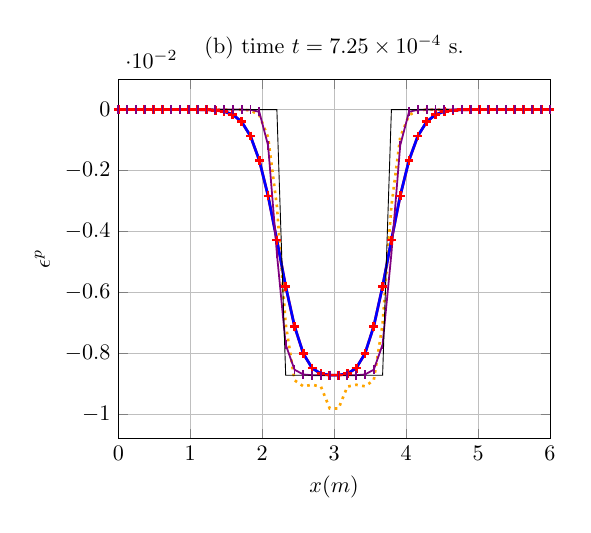
\begin{tikzpicture}[scale=0.8]
\begin{axis}[xlabel=$x (m)$,ylabel=$\epsilon^p$,ymajorgrids=true,xmajorgrids=true,legend pos=outer north east,title={(b) time $t = 7.25\times 10^{-4} $ s.},xmin=0.,xmax=6.]
\addplot[Red,very thick,mark=+,solid] coordinates {(0.0,-5.676632835751488e-19) (0.12244897959183673,-2.3898624238513766e-16) (0.24489795918367346,-3.735990751357306e-14) (0.36734693877551017,-2.3089144911084856e-12) (0.4897959183673469,-7.596762237094698e-11) (0.6122448979591837,-1.5415975357804979e-09) (0.7346938775510203,-1.0275730242331822e-08) (0.8571428571428571,-5.981932516353471e-08) (0.9795918367346939,-3.055798037968931e-07) (1.1020408163265305,-1.3747043608148892e-06) (1.2244897959183674,-5.4602719905226e-06) (1.346938775510204,-1.91823238251513e-05) (1.4693877551020407,-5.966726802674588e-05) (1.5918367346938775,-0.000164418651493838) (1.7142857142857142,-0.00040143744754996674) (1.836734693877551,-0.000868463225449077) (1.9591836734693877,-0.001665203797267752) (2.0816326530612246,-0.002832906100451628) (2.204081632653061,-0.004287995453610066) (2.326530612244898,-0.0058084443808726115) (2.4489795918367347,-0.007115753990208403) (2.571428571428571,-0.008016433919475449) (2.693877551020408,-0.008494471552590508) (2.816326530612245,-0.008677965053198252) (2.9387755102040813,-0.008723301560471332) (3.061224489795918,-0.008723301560471332) (3.183673469387755,-0.008677965053198252) (3.306122448979592,-0.00849447155259052) (3.4285714285714284,-0.008016433919475457) (3.5510204081632653,-0.007115753990208413) (3.673469387755102,-0.005808444380872623) (3.7959183673469385,-0.004287995453610076) (3.9183673469387754,-0.0028329061004516366) (4.040816326530612,-0.0016652037972677586) (4.163265306122449,-0.00086846322544908) (4.285714285714286,-0.0004014374475499613) (4.408163265306122,-0.00016441865149382611) (4.530612244897959,-5.9667268026732546e-05) (4.653061224489796,-1.918232382513086e-05) (4.775510204081632,-5.460271990507557e-06) (4.8979591836734695,-1.3747043608103478e-06) (5.020408163265306,-3.055798037929194e-07) (5.142857142857142,-5.981932515587126e-08) (5.26530612244898,-1.027573023324921e-08) (5.387755102040816,-1.5415975312391917e-09) (5.5102040816326525,-7.596762123562041e-11) (5.63265306122449,-2.308913923445202e-12) (5.755102040816326,-3.7358772187005907e-14) (5.877551020408163,-2.4097306387765065e-16) (6.0,-8.514949253627233e-19) };
\addplot[Orange,very thick,mark=none,dotted] coordinates {(0.0011999999999999927,0.0) (0.12359999999999997,0.0) (0.24599999999999994,0.0) (0.36839999999999995,0.0) (0.4907999999999999,-2.7815500895182294e-17) (0.6131999999999999,-3.8601103283110115e-17) (0.7355999999999999,-9.252911522274926e-17) (0.858,-1.5806584131150017e-15) (0.9803999999999998,-5.879373777480353e-14) (1.1027999999999998,-1.8355798153650192e-12) (1.2251999999999996,-4.7669529631024315e-11) (1.3475999999999997,-1.0242256048179808e-09) (1.4699999999999998,-1.8058382315295082e-08) (1.5923999999999996,-2.5837987508717037e-07) (1.7147999999999997,-2.955811391515107e-06) (1.8371999999999995,-2.650197421873382e-05) (1.9595999999999996,-0.00018124424208182778) (2.0819999999999994,-0.0009100274220600003) (2.2043999999999997,-0.0031724216849822393) (2.3267999999999995,-0.007051694130212292) (2.4491999999999994,-0.00889183395524355) (2.5715999999999997,-0.009090350906665956) (2.6939999999999995,-0.009040490458691425) (2.8163999999999993,-0.009101543401127671) (2.9387999999999996,-0.009819714666194801) (3.0611999999999995,-0.0098197146661948) (3.1835999999999993,-0.009101543401127772) (3.305999999999999,-0.009040490458691437) (3.4283999999999994,-0.009090350906665936) (3.5507999999999993,-0.008891833955243515) (3.673199999999999,-0.007051694130212307) (3.7955999999999994,-0.00317242168498228) (3.9179999999999993,-0.0009100274220600108) (4.040399999999999,-0.0001812442420818062) (4.1628,-2.6501974218710267e-05) (4.2852,-2.955811391528448e-06) (4.4076,-2.5837987506361237e-07) (4.53,-1.805838232863517e-08) (4.6524,-1.0242256082239605e-09) (4.7748,-4.766954637709118e-11) (4.8972,-1.835552283695766e-12) (5.0196,-5.885107176644462e-14) (5.142,-1.5667506626674108e-15) (5.2644,-6.897108895438059e-17) (5.3868,-1.7029898507254465e-18) (5.5092,-1.5043077014741444e-17) (5.6316,-1.7029898507254465e-18) (5.754,-1.4759245372953867e-17) (5.8764,-1.7029898507254465e-18) (5.9988,0.0) };
\addplot[Blue,very thick,mark=none,solid] coordinates {(0.0011999999999999927,0.0) (0.12359999999999997,-2.384185791015625e-16) (0.24599999999999994,-3.736019134521484e-14) (0.36839999999999995,-2.3089170455932617e-12) (0.4907999999999999,-7.596761584281921e-11) (0.6131999999999999,-1.5415975272655486e-09) (0.7355999999999999,-1.0275730234384537e-08) (0.858,-5.981932516098023e-08) (0.9803999999999998,-3.055798037946224e-07) (1.1027999999999998,-1.374704360806942e-06) (1.2251999999999996,-5.4602719905078414e-06) (1.3475999999999997,-1.9182323825132847e-05) (1.4699999999999998,-5.96672680267334e-05) (1.5923999999999996,-0.00016441865149382948) (1.7147999999999997,-0.000401437447549963) (1.8371999999999995,-0.0008684632254490853) (1.9595999999999996,-0.0016652037972677588) (2.0819999999999994,-0.002832906100451636) (2.2043999999999997,-0.00428799545361008) (2.3267999999999995,-0.005808444380872625) (2.4491999999999994,-0.007115753990208417) (2.5715999999999997,-0.00801643391947546) (2.6939999999999995,-0.008494471552590525) (2.8163999999999993,-0.00867796505319826) (2.9387999999999996,-0.008723301560471344) (3.0611999999999995,-0.008723301560471344) (3.1835999999999993,-0.00867796505319826) (3.305999999999999,-0.008494471552590525) (3.4283999999999994,-0.00801643391947546) (3.5507999999999993,-0.007115753990208417) (3.673199999999999,-0.005808444380872625) (3.7955999999999994,-0.00428799545361008) (3.9179999999999993,-0.002832906100451636) (4.040399999999999,-0.0016652037972677588) (4.1628,-0.0008684632254490853) (4.2852,-0.000401437447549963) (4.4076,-0.00016441865149382948) (4.53,-5.96672680267334e-05) (4.6524,-1.9182323825132847e-05) (4.7748,-5.4602719905078414e-06) (4.8972,-1.374704360806942e-06) (5.0196,-3.055798037946224e-07) (5.142,-5.981932516098023e-08) (5.2644,-1.0275730234384537e-08) (5.3868,-1.5415975272655486e-09) (5.5092,-7.596761584281921e-11) (5.6316,-2.3089170455932617e-12) (5.754,-3.736019134521484e-14) (5.8764,-2.384185791015625e-16) (5.9988,0.0) };
\addplot[Purple,thick,mark=|,solid] coordinates {(0.0011999999999999927,0.0) (0.12359999999999997,0.0) (0.24599999999999994,0.0) (0.36839999999999995,0.0) (0.4907999999999999,0.0) (0.6131999999999999,0.0) (0.7355999999999999,0.0) (0.858,-2.9802322387695314e-17) (0.9803999999999998,-1.329183578491211e-15) (1.1027999999999998,-4.1437149047851564e-14) (1.2251999999999996,-1.151418685913086e-12) (1.3475999999999997,-2.871338725090027e-11) (1.4699999999999998,-6.46675306558609e-10) (1.5923999999999996,-1.3273197644948959e-08) (1.7147999999999997,-2.510719147503376e-07) (1.8371999999999995,-4.397006492173672e-06) (1.9595999999999996,-7.414553616920114e-05) (2.0819999999999994,-0.0011776022671892642) (2.2043999999999997,-0.004734751896724993) (2.3267999999999995,-0.0077210124059583244) (2.4491999999999994,-0.008545394180645174) (2.5715999999999997,-0.008702161566804558) (2.6939999999999995,-0.008725895690329093) (2.8163999999999993,-0.008728522360980612) (2.9387999999999996,-0.008728709209868348) (3.0611999999999995,-0.008728709209868348) (3.1835999999999993,-0.008728522360980612) (3.305999999999999,-0.008725895690329093) (3.4283999999999994,-0.008702161566804558) (3.5507999999999993,-0.008545394180645174) (3.673199999999999,-0.0077210124059583244) (3.7955999999999994,-0.004734751896724993) (3.9179999999999993,-0.0011776022671892642) (4.040399999999999,-7.414553616920114e-05) (4.1628,-4.397006492173672e-06) (4.2852,-2.510719147562981e-07) (4.4076,-1.3273197644948959e-08) (4.53,-6.466753005981446e-10) (4.6524,-2.8713399171829228e-11) (4.7748,-1.1514246463775635e-12) (4.8972,-4.1437149047851564e-14) (5.0196,-1.329183578491211e-15) (5.142,-2.9802322387695314e-17) (5.2644,0.0) (5.3868,0.0) (5.5092,0.0) (5.6316,0.0) (5.754,0.0) (5.8764,0.0) (5.9988,0.0) };
\addplot[black,thin,mark=none,solid] coordinates {(0.0,-0.0) (0.12244897959183673,-0.0) (0.24489795918367346,-0.0) (0.36734693877551017,-0.0) (0.4897959183673469,-0.0) (0.6122448979591837,-0.0) (0.7346938775510203,-0.0) (0.8571428571428571,-0.0) (0.9795918367346939,-0.0) (1.1020408163265305,-0.0) (1.2244897959183674,-0.0) (1.346938775510204,-0.0) (1.4693877551020407,-0.0) (1.5918367346938775,-0.0) (1.7142857142857142,-0.0) (1.836734693877551,-0.0) (1.9591836734693877,-0.0) (2.0816326530612246,-0.0) (2.204081632653061,-0.0) (2.326530612244898,-0.008728715609439695) (2.4489795918367347,-0.008728715609439695) (2.571428571428571,-0.008728715609439695) (2.693877551020408,-0.008728715609439695) (2.816326530612245,-0.008728715609439695) (2.9387755102040813,-0.008728715609439695) (3.061224489795918,-0.008728715609439695) (3.183673469387755,-0.008728715609439695) (3.306122448979592,-0.008728715609439695) (3.4285714285714284,-0.008728715609439695) (3.5510204081632653,-0.008728715609439695) (3.673469387755102,-0.008728715609439695) (3.7959183673469385,-0.0) (3.9183673469387754,-0.0) (4.040816326530612,-0.0) (4.163265306122449,-0.0) (4.285714285714286,-0.0) (4.408163265306122,-0.0) (4.530612244897959,-0.0) (4.653061224489796,-0.0) (4.775510204081632,-0.0) (4.8979591836734695,-0.0) (5.020408163265306,-0.0) (5.142857142857142,-0.0) (5.26530612244898,-0.0) (5.387755102040816,-0.0) (5.5102040816326525,-0.0) (5.63265306122449,-0.0) (5.755102040816326,-0.0) (5.877551020408163,-0.0) (6.0,-0.0) };
%\legend{dgmpm,fem,fvm,fvm (SB),exact}
\end{axis}
\end{tikzpicture}
%%% Local Variables:
%%% mode: latex
%%% TeX-master: "../../mainManuscript"
%%% End:
}
%   {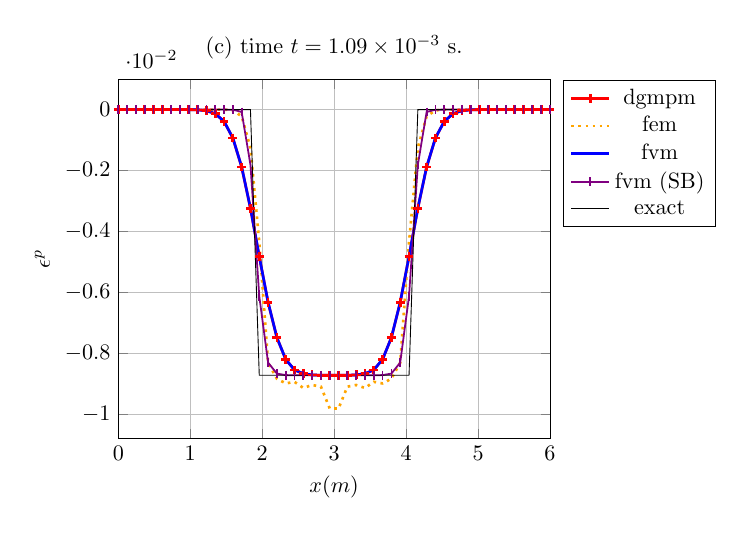
\begin{tikzpicture}[scale=0.8]
\begin{axis}[xlabel=$x (m)$,ylabel=$\epsilon^p$,ymajorgrids=true,xmajorgrids=true,legend pos=outer north east,title={(c) time $t = 1.09\times 10^{-3} $ s.},xmin=0.,xmax=6.]
\addplot[Red,very thick,mark=+,solid] coordinates {(0.0,-5.676632835751488e-19) (0.12244897959183673,-2.3898624238513766e-16) (0.24489795918367346,-3.735990751357306e-14) (0.36734693877551017,-2.3089144911084856e-12) (0.4897959183673469,-7.596762237094698e-11) (0.6122448979591837,-1.5415975357804979e-09) (0.7346938775510203,-2.1087029002110162e-08) (0.8571428571428571,-2.0628580472526095e-07) (0.9795918367346939,-1.5051975779320511e-06) (1.1020408163265305,-8.452232526292688e-06) (1.2244897959183674,-3.741900938747327e-05) (1.346938775510204,-0.00013315210803806102) (1.4693877551020407,-0.00038701776930482674) (1.5918367346938775,-0.0009319386970470464) (1.7142857142857142,-0.0018842066770200564) (1.836734693877551,-0.0032431409441831516) (1.9591836734693877,-0.004827293901207316) (2.0816326530612246,-0.00633202118341673) (2.204081632653061,-0.007489880430691718) (2.326530612244898,-0.008204526972019307) (2.4489795918367347,-0.008552921390073501) (2.571428571428571,-0.008674876019514461) (2.693877551020408,-0.008716486656783273) (2.816326530612245,-0.008726887116624966) (2.9387755102040813,-0.008728580772745199) (3.061224489795918,-0.008728580772745199) (3.183673469387755,-0.008726887116624966) (3.306122448979592,-0.00871648665678328) (3.4285714285714284,-0.008674876019514466) (3.5510204081632653,-0.008552921390073511) (3.673469387755102,-0.008204526972019318) (3.7959183673469385,-0.007489880430691721) (3.9183673469387754,-0.00633202118341673) (4.040816326530612,-0.0048272939012073204) (4.163265306122449,-0.0032431409441831525) (4.285714285714286,-0.001884206677020053) (4.408163265306122,-0.0009319386970470392) (4.530612244897959,-0.0003870177693048181) (4.653061224489796,-0.0001331521080380519) (4.775510204081632,-3.7419009387462476e-05) (4.8979591836734695,-8.452232526284741e-06) (5.020408163265306,-1.5051975779246716e-06) (5.142857142857142,-2.0628580471617835e-07) (5.26530612244898,-2.1087028991608393e-08) (5.387755102040816,-1.5415975312391917e-09) (5.5102040816326525,-7.596762123562041e-11) (5.63265306122449,-2.308913923445202e-12) (5.755102040816326,-3.7358772187005907e-14) (5.877551020408163,-2.4097306387765065e-16) (6.0,-8.514949253627233e-19) };
\addplot[Orange,very thick,mark=none,dotted] coordinates {(0.0011999999999999927,0.0) (0.12359999999999997,0.0) (0.24599999999999994,0.0) (0.36839999999999995,0.0) (0.4907999999999999,-2.7815500895182294e-17) (0.6131999999999999,-3.8601103283110115e-17) (0.7355999999999999,-2.0038513910202753e-16) (0.858,-1.7291875112624395e-14) (0.9803999999999998,-1.4890633878253755e-12) (1.1027999999999998,-8.711066870462328e-11) (1.2251999999999996,-3.5097774352346146e-09) (1.3475999999999997,-9.795044328882581e-08) (1.4699999999999998,-1.8896649221051307e-06) (1.5923999999999996,-2.4938869347233433e-05) (1.7147999999999997,-0.00022044973282056137) (1.8371999999999995,-0.0012586085323126788) (1.9595999999999996,-0.004366206064980092) (2.0819999999999994,-0.008315998828072487) (2.2043999999999997,-0.008841830788122323) (2.3267999999999995,-0.008995195469072521) (2.4491999999999994,-0.008944386605810638) (2.5715999999999997,-0.009146349400835571) (2.6939999999999995,-0.00904766889023616) (2.8163999999999993,-0.00910247337367582) (2.9387999999999996,-0.009819714666194801) (3.0611999999999995,-0.0098197146661948) (3.1835999999999993,-0.009102473373675955) (3.305999999999999,-0.009047668890236175) (3.4283999999999994,-0.009146349400835545) (3.5507999999999993,-0.008944386605810636) (3.673199999999999,-0.008995195469072475) (3.7955999999999994,-0.00884183078812235) (3.9179999999999993,-0.008315998828072471) (4.040399999999999,-0.004366206064980109) (4.1628,-0.0012586085323127117) (4.2852,-0.00022044973282050575) (4.4076,-2.4938869347250462e-05) (4.53,-1.8896649221051307e-06) (4.6524,-9.795044333225205e-08) (4.7748,-3.5097774522645135e-09) (4.8972,-8.711060172035581e-11) (5.0196,-1.4891476858229865e-12) (5.142,-1.7265194938296362e-14) (5.2644,-1.9045103163946243e-16) (5.3868,-1.7029898507254465e-18) (5.5092,-1.5043077014741444e-17) (5.6316,-1.7029898507254465e-18) (5.754,-1.4759245372953867e-17) (5.8764,-1.7029898507254465e-18) (5.9988,0.0) };
\addplot[Blue,very thick,mark=none,solid] coordinates {(0.0011999999999999927,0.0) (0.12359999999999997,-2.384185791015625e-16) (0.24599999999999994,-3.736019134521484e-14) (0.36839999999999995,-2.3089170455932617e-12) (0.4907999999999999,-7.596761584281921e-11) (0.6131999999999999,-1.5415975272655486e-09) (0.7355999999999999,-2.1087028992176057e-08) (0.858,-2.0628580471873284e-07) (0.9803999999999998,-1.5051975779294967e-06) (1.1027999999999998,-8.452232526284456e-06) (1.2251999999999996,-3.741900938746333e-05) (1.3475999999999997,-0.00013315210803804993) (1.4699999999999998,-0.00038701776930482386) (1.5923999999999996,-0.0009319386970470428) (1.7147999999999997,-0.001884206677020061) (1.8371999999999995,-0.003243140944183153) (1.9595999999999996,-0.004827293901207322) (2.0819999999999994,-0.006332021183416736) (2.2043999999999997,-0.007489880430691725) (2.3267999999999995,-0.008204526972019321) (2.4491999999999994,-0.008552921390073513) (2.5715999999999997,-0.008674876019514464) (2.6939999999999995,-0.008716486656783276) (2.8163999999999993,-0.008726887116624964) (2.9387999999999996,-0.008728580772745204) (3.0611999999999995,-0.008728580772745204) (3.1835999999999993,-0.008726887116624964) (3.305999999999999,-0.008716486656783276) (3.4283999999999994,-0.008674876019514464) (3.5507999999999993,-0.008552921390073513) (3.673199999999999,-0.008204526972019321) (3.7955999999999994,-0.007489880430691725) (3.9179999999999993,-0.006332021183416736) (4.040399999999999,-0.004827293901207322) (4.1628,-0.003243140944183153) (4.2852,-0.001884206677020061) (4.4076,-0.0009319386970470428) (4.53,-0.00038701776930482386) (4.6524,-0.00013315210803804993) (4.7748,-3.741900938746333e-05) (4.8972,-8.452232526284456e-06) (5.0196,-1.5051975779294967e-06) (5.142,-2.0628580471873284e-07) (5.2644,-2.1087028992176057e-08) (5.3868,-1.5415975272655486e-09) (5.5092,-7.596761584281921e-11) (5.6316,-2.3089170455932617e-12) (5.754,-3.736019134521484e-14) (5.8764,-2.384185791015625e-16) (5.9988,0.0) };
\addplot[Purple,thick,mark=|,solid] coordinates {(0.0011999999999999927,0.0) (0.12359999999999997,0.0) (0.24599999999999994,0.0) (0.36839999999999995,0.0) (0.4907999999999999,0.0) (0.6131999999999999,0.0) (0.7355999999999999,0.0) (0.858,-2.8014183044433593e-16) (0.9803999999999998,-2.1100044250488282e-14) (1.1027999999999998,-1.2365996837615966e-12) (1.2251999999999996,-5.9033864736557e-11) (1.3475999999999997,-2.3761736869812012e-09) (1.4699999999999998,-8.325840687155723e-08) (1.5923999999999996,-2.6323343349337577e-06) (1.7147999999999997,-7.853228000084162e-05) (1.8371999999999995,-0.0018212430710175336) (1.9595999999999996,-0.006137739318747551) (2.0819999999999994,-0.008311894308815801) (2.2043999999999997,-0.008672824985492957) (2.3267999999999995,-0.008722601697817814) (2.4491999999999994,-0.00872819127980076) (2.5715999999999997,-0.008728663911155045) (2.6939999999999995,-0.008728711882144921) (2.8163999999999993,-0.008728715435078365) (2.9387999999999996,-0.0087287156054703) (3.0611999999999995,-0.0087287156054703) (3.1835999999999993,-0.008728715435078365) (3.305999999999999,-0.008728711882144921) (3.4283999999999994,-0.008728663911155045) (3.5507999999999993,-0.00872819127980076) (3.673199999999999,-0.008722601697817814) (3.7955999999999994,-0.008672824985492957) (3.9179999999999993,-0.008311894308815794) (4.040399999999999,-0.006137739318747556) (4.1628,-0.0018212430710175217) (4.2852,-7.853228000084758e-05) (4.4076,-2.6323343349575996e-06) (4.53,-8.325840684175491e-08) (4.6524,-2.37617369890213e-09) (4.7748,-5.903387665748596e-11) (4.8972,-1.2365996837615966e-12) (5.0196,-2.1100044250488282e-14) (5.142,-2.8014183044433593e-16) (5.2644,0.0) (5.3868,0.0) (5.5092,0.0) (5.6316,0.0) (5.754,0.0) (5.8764,0.0) (5.9988,0.0) };
\addplot[black,thin,mark=none,solid] coordinates {(0.0,-0.0) (0.12244897959183673,-0.0) (0.24489795918367346,-0.0) (0.36734693877551017,-0.0) (0.4897959183673469,-0.0) (0.6122448979591837,-0.0) (0.7346938775510203,-0.0) (0.8571428571428571,-0.0) (0.9795918367346939,-0.0) (1.1020408163265305,-0.0) (1.2244897959183674,-0.0) (1.346938775510204,-0.0) (1.4693877551020407,-0.0) (1.5918367346938775,-0.0) (1.7142857142857142,-0.0) (1.836734693877551,-0.0) (1.9591836734693877,-0.008728715609439695) (2.0816326530612246,-0.008728715609439695) (2.204081632653061,-0.008728715609439695) (2.326530612244898,-0.008728715609439695) (2.4489795918367347,-0.008728715609439695) (2.571428571428571,-0.008728715609439695) (2.693877551020408,-0.008728715609439695) (2.816326530612245,-0.008728715609439695) (2.9387755102040813,-0.008728715609439695) (3.061224489795918,-0.008728715609439695) (3.183673469387755,-0.008728715609439695) (3.306122448979592,-0.008728715609439695) (3.4285714285714284,-0.008728715609439695) (3.5510204081632653,-0.008728715609439695) (3.673469387755102,-0.008728715609439695) (3.7959183673469385,-0.008728715609439695) (3.9183673469387754,-0.008728715609439695) (4.040816326530612,-0.008728715609439695) (4.163265306122449,-0.0) (4.285714285714286,-0.0) (4.408163265306122,-0.0) (4.530612244897959,-0.0) (4.653061224489796,-0.0) (4.775510204081632,-0.0) (4.8979591836734695,-0.0) (5.020408163265306,-0.0) (5.142857142857142,-0.0) (5.26530612244898,-0.0) (5.387755102040816,-0.0) (5.5102040816326525,-0.0) (5.63265306122449,-0.0) (5.755102040816326,-0.0) (5.877551020408163,-0.0) (6.0,-0.0) };
\legend{dgmpm,fem,fvm,fvm (SB),exact}
\end{axis}
\end{tikzpicture}
%%% Local Variables:
%%% mode: latex
%%% TeX-master: "../../mainManuscript"
%%% End:
}
%   \caption{elastic-plastic RP epsp}
%   \label{fig:epsp_elastoplastic_RP}
% \end{figure}


%%% Local Variables:
%%% mode: latex
%%% TeX-master: "../mainManuscript"
%%% End: